\documentclass[a4paper]{article}
\usepackage[T1]{fontenc}			      % \chapter package
\usepackage[english]{babel}
\usepackage[english]{isodate}  		  % date format
\usepackage{graphicx}				        % manage images
\usepackage{amsfonts}
\usepackage{booktabs}				        % high quality tables
\usepackage{amsmath}				        % math package
\usepackage{amssymb}				        % another math package (e.g. \nexists)
\usepackage{bm}                     % bold math symbols
\usepackage{mathtools}				      % emphasize equations
\usepackage{stmaryrd} 				      % '\llbracket' and '\rrbracket'
\usepackage{amsthm}					        % better theorems
\usepackage{enumitem}				        % manage list
\usepackage{pifont}					        % nice itemize
\usepackage{cancel}					        % cancel math equations
\usepackage{caption}				        % custom caption
\usepackage[]{mdframed}				      % box text
\usepackage{multirow}				        % more lines in a table
\usepackage{textcomp, gensymb}		  % degree symbol
\usepackage[x11names]{xcolor}		    % RGB color
\usepackage[many]{tcolorbox}		    % colorful box
\usepackage{multicol}				        % more rows in a table (used for the lists)
\usepackage{listings}
\usepackage{url}
\usepackage{qrcode}
\usepackage{fontawesome5}           % https://fontawesome.com/v5/search?ic=free&o=r
\usepackage{ragged2e}
\usepackage{cite}                   % references
\usepackage{imakeidx}               % index
\usepackage{mfirstuc}               % first letter uppercase
\makeindex[program=makeindex, columns=1,
           title=Index, 
           intoc,
           options={-s index-style.ist}]
\usepackage{fancyhdr}
\usepackage{soul}                   % highlight text (as a highlighter)
\usepackage{adjustbox}              % avoid table overfull
\usepackage{tikz}
% \usetikzlibrary{positioning}
\usetikzlibrary{arrows.meta, positioning, calc}

% ~ Dark Mode ~
% \usepackage{pagecolor}      % For background color
% \pagecolor{black}           % Background color
% \color{white}               % Default text color
% \sethlcolor{darkgray}
% \usepackage[colorlinks=true, linkcolor=cyan, urlcolor=cyan]{hyperref} % dark mode

\definecolor{codegreen}{rgb}{0,0.6,0}
\definecolor{codegray}{rgb}{0.5,0.5,0.5}
\definecolor{codepurple}{rgb}{0.58,0,0.82}
\definecolor{backcolour}{rgb}{0.95,0.95,0.92}
\lstdefinelanguage{misc}
{
  % list of keywords
  morekeywords={%
    add,
    addi,
    lw,
    sw,
    beq,
    bne,
    j,
    jr,
    offset,
    sub,
    and,
    or
  },
  sensitive=false, % keywords are not case-sensitive
  morecomment=[l]{\#}, % l is for line comment
  % morecomment=[s]{/*}{*/}, % s is for start and end delimiter
  % morestring=[b]" % defines that strings are enclosed in double quotes
}
\lstdefinelanguage{unknown}
{
  % list of keywords
  morekeywords={%
    addd,
    addi,
    divd,
    sd,
    muld,
    multd,
    ld,
    subd,
    subi,
    bnez,
    bne
  },
  sensitive=false, % keywords are not case-sensitive
  morecomment=[l]{;}, % l is for line comment
  morecomment=[l]{\#}, % l is for line comment
  % morecomment=[s]{/*}{*/}, % s is for start and end delimiter
  % morestring=[b]" % defines that strings are enclosed in double quotes
}
\lstdefinelanguage{riscv}
{
  % list of keywords
  morekeywords={%
    add,
    addi,
    ld,
    sd,
    offset,
    beq,
    bne,
    j,
    jr,
    nop,
    sub,
    subi,
    and,
    mov
  },
  sensitive=false, % keywords are not case-sensitive
  morecomment=[l]{\#}, % l is for line comment
  % morecomment=[s]{/*}{*/}, % s is for start and end delimiter
  % morestring=[b]" % defines that strings are enclosed in double quotes
}
\lstdefinestyle{mystyle}{
    backgroundcolor=\color{backcolour},
    commentstyle=\color{codegreen},
    keywordstyle=\color{magenta},
    numberstyle=\tiny\color{codegray},
    stringstyle=\color{codepurple},
    basicstyle=\ttfamily\footnotesize,
    breakatwhitespace=false,
    breaklines=true,
    captionpos=b,
    keepspaces=true,
    numbers=left,
    numbersep=5pt,
    showspaces=false,
    showstringspaces=false,
    showtabs=false,
    tabsize=2
}
\lstset{style=mystyle}


% thanks Mico: https://tex.stackexchange.com/a/60218/312896
\makeatletter
\renewcommand\paragraph{\@startsection{paragraph}{4}{\z@}%
            {-2.5ex\@plus -1ex \@minus -.25ex}%
            {1.25ex \@plus .25ex}%
            {\normalfont\normalsize\bfseries}}
\makeatother
\setcounter{secnumdepth}{4} % how many sectioning levels to assign numbers to
\setcounter{tocdepth}{4}    % how many sectioning levels to show in ToC


% draw a frame around given text
\newcommand{\framedtext}[1]{%
	\par%
	\noindent\fbox{%
		\parbox{\dimexpr\linewidth-2\fboxsep-2\fboxrule}{#1}%
	}%
}


% table of content links
\usepackage{xcolor}
\usepackage[linkcolor=black, citecolor=blue, urlcolor=cyan]{hyperref} % hypertexnames=false
\hypersetup{
	colorlinks=true
}


\newtheorem{theorem}{\textcolor{Red3}{\underline{Theorem}}}
\renewcommand{\qedsymbol}{QED}
\newcommand{\dquotes}[1]{``#1''}
\newcommand{\important}[1]{\textcolor{red}{\textbf{#1}}}
\newcommand{\longline}{\noindent\rule{\textwidth}{0.4pt}}
\newcommand{\circledtext}[1]{\raisebox{.5pt}{\textcircled{\raisebox{-.9pt}{#1}}}}
\newcommand{\definition}[1]{\textcolor{Red3}{\textbf{#1}}\index{#1}}
\newcommand{\example}[1]{\textcolor{Green4}{\textbf{#1}}}
\newcommand{\highspace}{\vspace{1.2em}\noindent}
% I never remember every icon, so I use custom commands to do this
\newcommand{\speedIcon}{tachometer-alt}
\newcommand{\definitionWithSpecificIndex}[3]{\textcolor{Red3}{\textbf{#1}}\index{#2}\index{#3}}
\newcommand{\hqlabel}[2]{\label{#1}\hypertarget{#1}{#2}}
\newcommand{\hqpageref}[1]{\hyperlink{#1}{\hypergetpageref{#1}}}
\newcommand{\answer}{\textcolor{Green3}{\textbf{\emph{Answer: }}}}
\newcommand{\version}{v0.12.0}

% \includeonly{
%   sections/advanced-memory/introduction,
%   sections/advanced-memory/principle-of-locality,
%   sections/advanced-memory/so-what-is-a-cache,
%   sections/advanced-memory/cache-performance-metrics,
%   sections/advanced-memory/cache-architecture/cache-architecture,
%   sections/advanced-memory/cache-architecture/block-placement,
%   sections/advanced-memory/cache-architecture/block-identifiation,
%   sections/advanced-memory/cache-architecture/replacement-strategy,
%   sections/advanced-memory/cache-architecture/write-strategy,
%   sections/advanced-memory/miss-penalty-reduction,
%   sections/advanced-memory/design-space-of-cache,
%   %
%   sections/advanced-memory/cache-miss-classification,
%   sections/advanced-memory/improving-cache-performance/improving-cache-performance,
%   sections/advanced-memory/improving-cache-performance/reducing-miss-rate-techniques/increasing-cache-size,
%   sections/advanced-memory/improving-cache-performance/reducing-miss-rate-techniques/increasing-block-size,
%   sections/advanced-memory/improving-cache-performance/reducing-miss-rate-techniques/increasing-associativity,
%   sections/advanced-memory/improving-cache-performance/reducing-miss-rate-techniques/victim-cache,
%   sections/advanced-memory/improving-cache-performance/reducing-miss-rate-techniques/pseudo-associativity-and-way-prediction,
%   sections/advanced-memory/improving-cache-performance/reducing-miss-rate-techniques/hardware-prefetching,
%   sections/bibliography-and-index
% }


\begin{document}
    \newcounter{definition}[section]
    \newcounter{example}[section]
    \newcounter{takeaways}[section]
    
    \newtcolorbox[use counter = definition]{definitionbox}[1][]{%
        breakable,
        enhanced,
        colback=red!5!white,
        colframe=red!75!black,
        fonttitle=\bfseries,
        title={Definition \thetcbcounter #1} %
    }
    
    \newtcolorbox[use counter = example]{examplebox}[1][]{%
        breakable,
        enhanced,
        colback=Green4!5!white,
        colframe=Green4!75!black,
        fonttitle=\bfseries,
        title={Example \thetcbcounter #1} %
    }

    \newtcolorbox[use counter = takeaways]{takeawaysbox}[1][]{%
        breakable,
        enhanced,
        colback=Green3!5!white,
        colframe=Green3!75!black,
        fonttitle=\bfseries,
        title={Key Takeaways#1} %
    }

    \newtcolorbox[]{deepeningbox}[1][]{%
        breakable,
        enhanced,
        colback=DarkOrange3!5!white,
        colframe=DarkOrange3!75!black,
        fonttitle=\bfseries,
        title={Deepening#1} %
    }
	
    %%%%%%%%%%%%%%%
    % Notes cover %
    %%%%%%%%%%%%%%%
    \author{260236}
\title{Quantum Computing - Notes - \version}
\date{\printdayoff\today}
\maketitle

    %%%%%%%%%%%
    % Preface %
    %%%%%%%%%%%
    \section*{Preface}

Every theory section in these notes has been taken from two sources:
\begin{itemize}
    \item Ian Goodfellow and Yoshua Bengio and Aaron Courville, \href{https://www.deeplearningbook.org/}{Deep Learning}, MIT Press. \cite{Goodfellow-et-al-2016}
    \item Course slides.\cite{course-slides-polimi}
\end{itemize}
About:
\begin{itemize}
    \item[\faIcon{github}] \href{https://github.com/PoliMI-HPC-E-notes-projects-AndreVale69/HPC-E-PoliMI-university-notes}{GitHub repository}
    \begin{center}
        \qrcode{https://github.com/PoliMI-HPC-E-notes-projects-AndreVale69/HPC-E-PoliMI-university-notes}
    \end{center}
\end{itemize}
These notes are an unofficial resource and shouldn't replace the course material or any other book on artificial neural networks and deep learning. It is not made for commercial purposes. I've made the following notes to help me improve my knowledge and maybe it can be helpful for everyone.

As I have highlighted, a student should choose the teacher's material or a book on the topic. These notes can only be a helpful material.

\highspace
During the Artificial Neural Networks and Deep Learning course, me and my other three colleagues Alberto Ondei, \href{https://it.linkedin.com/in/javedabdullah}{Abdullah Javed} and \href{https://www.hpc.cineca.it/staff/barbari-filippo/}{Filippo Barbari}, we created two projects:
\begin{itemize}
    \item[\faIcon{github}] \href{https://github.com/PoliMI-HPC-E-notes-projects-AndreVale69/AN2DL-Challenge-1}{Time Series Classification}. Deep Neural Netowrk (TCN $+$ BiLSTM with Attention) model on multivariate time-series classification.
    \begin{center}
        \qrcode{https://github.com/PoliMI-HPC-E-notes-projects-AndreVale69/AN2DL-Challenge-1}
    \end{center}
    \item[\faIcon{github}] \href{https://github.com/PoliMI-HPC-E-notes-projects-AndreVale69/AN2DL-Challenge-2}{Image Classification}. Histopathology image classification to predict molecular subtypes.
    \begin{center}
        \qrcode{https://github.com/PoliMI-HPC-E-notes-projects-AndreVale69/AN2DL-Challenge-2}
    \end{center}
\end{itemize}

    %%%%%%%%%%%%%%%%%%%%%
    % Table of contents %
    %%%%%%%%%%%%%%%%%%%%%
	  \tableofcontents
    \newpage

    %%%%%%%%%%%%%%%%%%%
    % Fancy pagestyle %
    %%%%%%%%%%%%%%%%%%%
    \pagestyle{fancy}
    \fancyhead{} % clear all header fields
    \fancyhead[R]{\nouppercase{\leftmark\hfill\rightmark}}
    \setlength{\headheight}{22.48724pt}
    \addtolength{\topmargin}{-10.48724pt}

    %%%%%%%%%%%%%%%%%%
    % Basic concepts %
    %%%%%%%%%%%%%%%%%%
    \section{Pipelining}

\subsection{Basic Concepts}

\definition{Pipelining} is a fundamental \textbf{technique} in computer architecture aimed at \textbf{improving instruction throughput by overlapping the execution of multiple instructions}. The main idea behind pipelining is to \hl{divide the execution of an instruction into distinct stages and process different instructions simultaneously in these stages}. This approach significantly increases the efficiency of instruction execution in modern processors.

\highspace
\begin{flushleft}
    \textcolor{Green3}{\faIcon{tools} \textbf{Understanding the RISC-V instruction set}}
\end{flushleft}
Before delving into pipelining, it is essential to understand the \textbf{basic instruction set} of the RISC-V architecture. The instruction set consists of three major categories:
\begin{itemize}
    \item \important{ALU Instructions (Arithmetic and Logic Operations)}
    \begin{itemize}
        \item Performs \textbf{addition between registers}:
        \begin{lstlisting}[language=riscv]
add rd, rs1, rs2\end{lstlisting}
        Performs the addition between the values in registers \texttt{rs1} and \texttt{rs2} and stores the result in register \texttt{rd}.
        \begin{equation*}
            \texttt{rd} \leftarrow \texttt{rs1} + \texttt{rs2}
        \end{equation*}

        \item Performs an \textbf{addition between a constant and a register}:
        \begin{lstlisting}[language=riscv]
addi rd, rs1, 4\end{lstlisting}
        Performs the addition between the value in register \texttt{rs1} and the value \texttt{4} and stores the result in register \texttt{rd}.
        \begin{equation*}
            \texttt{rd} \leftarrow \texttt{rs1} + \texttt{4}
        \end{equation*}
    \end{itemize}

    \item \important{Load/Store Instructions (Memory Operations)}
    \begin{itemize}
        \item \textbf{Loads} data from memory:
        \begin{lstlisting}[language=riscv]
ld rd, offset(rs1)\end{lstlisting}
        Load data into register \texttt{rd} from an address formed by adding \texttt{rs1} to a signed \texttt{offset}.
        \begin{equation*}
            \texttt{rd} \leftarrow M\left[\texttt{rs1} + \texttt{offset}\right]
        \end{equation*}

        \item \textbf{Stores} data in memory:
        \begin{lstlisting}[language=riscv]
sd rs2, offset(rs1)\end{lstlisting}
        Store data from register \texttt{rs2} to an address formed by adding \textsl{rs1} to a signed \textsl{offset}.
        \begin{equation*}
            M\left[\texttt{rs1} + \texttt{offset}\right] \leftarrow \texttt{rs2}
        \end{equation*}
    \end{itemize}

    \newpage

    \item \important{Branching Instructions (Control Flow Management)}
    \begin{itemize}
        \item \important{Conditional Branches}
        \begin{itemize}
            \item Branch on equal:
            \begin{lstlisting}[language=riscv]
beq rs1, rs2, L1\end{lstlisting}
            Branch to the label \texttt{L1} if the value in register \texttt{rs1} is equal to the value in register \texttt{rs2}.
            \begin{equation*}
                \texttt{rs1} = \texttt{rs1} \xRightarrow{\text{go to}} \texttt{L1}
            \end{equation*}
            \item Branch on not equal:
            \begin{lstlisting}[language=riscv]
bne rs1, rs2, L1\end{lstlisting}
            Branch to the label \texttt{L1} if the value in register \texttt{rs1} is not equal to the value in register \texttt{rs2}.
            \begin{equation*}
                \texttt{rs1} \ne \texttt{rs2} \xRightarrow{\text{go to}} \texttt{L1}
            \end{equation*}
        \end{itemize}
        \item \important{Unconditional Jumps}
        \begin{itemize}
            \item Jump to the label (jump):
            \begin{lstlisting}[language=riscv]
j L1\end{lstlisting}
            Jump directly to the \texttt{L1} label.
            \item Jump to the address stored in a register (jump register):
            \begin{lstlisting}[language=riscv]
jr ra\end{lstlisting}
            Take the value in register \texttt{ra} and use it as the address to jump to. So it is assumed that \texttt{ra} contains an address.
        \end{itemize}
    \end{itemize}
\end{itemize}
These basic instructions will be used throughout the course.

\highspace
\begin{flushleft}
    \textcolor{Green3}{\faIcon{stream} \textbf{Execution phases in RISC-V}}
\end{flushleft}
\begin{enumerate}
    \item \definition{IF (Instruction Fetch)}: The instruction is \textbf{fetched} from memory.
    \item \definition{ID (Instruction Decode)}: The instruction is \textbf{decoded}, and the \textbf{required registers are read}.
    \item \definition{EX (Execution)}: The instruction is \textbf{executed}, typically involving ALU operations.
    \item \definition{ME (Memory Access)}: For \emph{load}/\emph{store} instructions, this stage \textbf{reads from} or \textbf{writes to} memory.
    \item \definition{WB (Write Back)}: The \textbf{result is written back} to the destination register.
\end{enumerate}
These five stages form the basis of the RISC-V pipeline.

\newpage

\begin{flushleft}
    \textcolor{Green3}{\faIcon{tools} \textbf{Implementation of the RISC-V Data Path}}
\end{flushleft}
The \definition{RISC-V Data Path} is a fundamental component of the processor's architecture, responsible for \textbf{executing instructions efficiently by coordinating various hardware units}. It defines how instructions flow through different stages of execution, interacting with memory, registers, and the Arithmetic Logic Unit (ALU).

\begin{figure}[!htp]
    \centering
    \includegraphics[width=\textwidth]{img/generic-risc-v-dp.pdf}
    \caption{Generic implementation of the RISC-V Data Path.}
\end{figure}

\begin{figure}[!htp]
    \centering
    \includegraphics[width=\textwidth]{img/detailed-risc-v-dp.pdf}
    \caption{Specific implementation of the RISC-V Data Path.}
\end{figure}

\noindent
Its fundamental components include:
\begin{itemize}
    \item \important{Instruction Memory and Data Memory Separation}. RISC-V\break adopts a Harvard Architecture style, where the \textbf{Instruction Memory (IM)} and \textbf{Data Memory (DM) are separate}. This \textbf{prevents structural hazards} where instruction fetch and memory access could conflict in a single-memory design (this topic will be addressed later).

    \item \important{General-Purpose Register File (RF)}. It consists of \textbf{32 registers}, each \textbf{32-bit} wide. The register file has \textbf{two read ports} and \textbf{one write port} to \hl{support simultaneous read and write operations}. This setup allows faster register access, which is crucial for pipelined execution.

    \item \important{Program Counter (PC)}. It \textbf{holds the address of the next instruction to be fetched}. Automatically increments during execution, typically by 4 bytes (for 32-bit instructions).
    
    \item \important{Arithmetic Logic Unit (ALU)}. \textbf{Performs arithmetic and logical operations} required by instructions. Inputs to the ALU come from registers or immediate values decoded from the instruction.
\end{itemize}
Other components that we can see in the general implementation of the RISC-V data path are:
\begin{itemize}
    \item \textbf{Register File}. \hl{Stores temporary values used by instructions}. Contains read ports (two registers can be read simultaneously for ALU operations) and write port (one register can be updated per clock cycle). The register file ensures high-speed execution of operations by reducing memory accesses.
    \item \textbf{Instruction Fetch (IF)}. The PC (Program Counter) retrieves the next instruction from Instruction Memory. The PC is incremented using an adder (\texttt{PC + 4}), ensuring sequential instruction flow.
    \item \textbf{Instruction Decode (ID)}. Extracts opcode (determines the instruction type), source and destination registers, immediate values (if present). It \hl{reads values from the Register File based on instruction requirements}.
    \item \textbf{Execution (EX)}. The \hl{ALU performs arithmetic and logical operations}. A multiplexer (MUX) selects the second operand: a register value (for R-type instructions) or an immediate value (for I-type instructions like \texttt{addi}). The \hl{ALU result is forwarded} to the next stage.
    \item \textbf{Memory Access (ME)}. Load (\texttt{ld}) and Store (\texttt{sd}) instructions interact with data memory. Data is either \textbf{loaded from memory into a register} or \textbf{stored from a register into memory}.
    \item \textbf{Write Back (WB)}. The result from ALU or memory is \textbf{written back to the Register File}.
\end{itemize}

\newpage

\begin{examplebox}[: Data Path Execution Example]
    Let's consider a simple RISC-V \textbf{load instruction} (\texttt{ld x10, 40(x1)}) passing through the data path:
    \begin{enumerate}
        \item \textbf{IF Stage}: Instruction Fetch
        \begin{itemize}
            \item \texttt{PC} $\rightarrow$ Instruction Memory $\rightarrow$ \texttt{ld x10, 40(x1)} fetched
            \item \texttt{PC} updated to \texttt{PC + 4}
        \end{itemize}

        \item \textbf{ID Stage}: Instruction Decode
        \begin{itemize}
            \item Registers read: \texttt{x1} (base register for memory access)
            \item Immediate value extracted: \texttt{40}
        \end{itemize}

        \item \textbf{EX Stage}: Execution
        \begin{itemize}
            \item ALU calculates memory address: \texttt{x1 + 40}
        \end{itemize}

        \item \textbf{ME Stage}: Memory Access
        \begin{itemize}
            \item Data is loaded from \texttt{M[x1 + 40]}
        \end{itemize}

        \item \textbf{WB Stage}: Write Back
        \begin{itemize}
            \item Data stored in \texttt{x10}
        \end{itemize}
    \end{enumerate}
\end{examplebox}

    \subsection{RISC-V Pipelining}

Pipelining is analogous to an assembly line in a factory. Instead of waiting for one instruction to complete before starting the next, \textbf{different instructions are executed simultaneously in different stages}.

\highspace
If we consider a \textbf{non-pipelined execution}:
\begin{itemize}
    \item Each instruction completes all five stages sequentially before the next instruction starts.
    \item If each instruction stage (IF stage, ID stage, etc.) takes, say, 2 nanoseconds, executing all stages of an instruction (IF, ID, EX, MEM, WB) takes 5 times 2 nanoseconds, then 10 nanoseconds. If we also want to execute 5 instructions, we need 10 nanoseconds times 5, then 50 nanoseconds!
\end{itemize}
Now, we consider a \textbf{pipelined execution}:
\begin{itemize}
    \item Once the first instruction moves to the second stage, the next instruction starts in the first stage.
    \item The \textbf{pipeline becomes fully utilized} after the first few cycles, significantly \textbf{improving throughput}.
\end{itemize}
In an \textbf{ideal scenario}, a 5-stage pipeline should provide a speedup of $5\times$ reducing execution time to:
\begin{equation*}
    \left(5+4\right) \times 2 \text{ ns } = 18 \text{ ns}
\end{equation*}
Where $5$ are the steps of the first instruction, $5$ are the steps of the last instruction, minus $1$ because one step is already counted in the first instruction, so $4$. Therefore, $9$ is multiplied by $2$ nanoseconds, the time taken by each stage. The result, $18$ nanoseconds, is the time it takes the pipeline to execute 5 instructions in an ideal scenario.

\begin{figure}[!htp]
    \centering
    \includegraphics[width=\textwidth]{img/sequential-vs-pipelining-1.pdf}
    \caption{Sequential vs. Pipelining execution.}
\end{figure}

\newpage

\begin{flushleft}
    \textcolor{Green3}{\faIcon{\speedIcon} \textbf{Pipeline Performance and Speedup}}
\end{flushleft}
The ideal performance improvement from pipelining is derived from the fact that \textbf{once the pipeline is filled}, \textbf{a new instruction completes every cycle}. The key performance metrics include:
\begin{itemize}
    \item \textbf{Latency (Execution Time)}: The total time to complete a single instruction does not change (sequential or pipeline).
    \item \textbf{Throughput (Instructions per Unit Time)}: The number of completed instruction per unit time significantly increases.
    \item \textbf{Speedup Calculation}
    \begin{itemize}
        \item A non-pipelined CPU with 5 execution cycles of 2 ns would take 10 ns per instruction.
        \item A pipelined CPU with 5 stages of 2 ns results in 1 instruction completing every 2 ns.
        \item This gives a theoretical speedup of $5\times$ (ideal case).
    \end{itemize}
\end{itemize}
Unfortunately, real-world implementations are subject to \textbf{pipeline hazards} that reduce efficiency.

\newpage

\begin{flushleft}
    \textcolor{Green3}{\faIcon{book} \textbf{Understanding Pipelining Performance}}
\end{flushleft}
Pipelining \textbf{improves instruction throughput} by allowing multiple instructions to be processed simultaneously in different stages. The \textbf{execution of an instruction is divided into 5 pipeline stages}:
\begin{enumerate}
    \item IF (Instruction Fetch)
    \item ID (Instruction Decode)
    \item EX (Execution)
    \item MEM (Memory Access)
    \item WB (Write Back)
\end{enumerate}
\textbf{Each stage takes 2 ns} (a \emph{pipeline cycle}), meaning that an \textbf{instruction moves from one stage to the next every 2 ns}. Now, let's analyze the timeline of instruction execution:
\begin{table}[!htp]
    \centering
    \begin{tabular}{@{} l | c | c | c | c | c @{}}
        \toprule
        \textbf{Clock Cycle} & \textbf{IF} & \textbf{ID} & \textbf{EX} & \textbf{MEM} & \textbf{WB} \\
        \midrule
        1st  (0-2 ns)   & \texttt{I1} &    &    &    &    \\ [.3em]
        2nd  (2-4 ns)   & \texttt{I2} & \texttt{I1} &    &    &    \\ [.3em]
        3rd  (4-6 ns)   & \texttt{I3} & \texttt{I2} & \texttt{I1} &    &    \\ [.3em]
        4th  (6-8 ns)   & \texttt{I4} & \texttt{I3} & \texttt{I2} & \texttt{I1} &    \\ [.3em]
        5th  (8-10 ns)  & \texttt{I5} & \texttt{I4} & \texttt{I3} & \texttt{I2} & \texttt{I1} \\ [.3em]
        6th  (10-12 ns) & \texttt{I6} & \texttt{I5} & \texttt{I4} & \texttt{I3} & \texttt{I2} \\ [.3em]
        7th  (12-14 ns) & \texttt{I7} & \texttt{I6} & \texttt{I5} & \texttt{I4} & \texttt{I3} \\ [.3em]
        8th  (14-16 ns) & \texttt{I8} & \texttt{I7} & \texttt{I6} & \texttt{I5} & \texttt{I4} \\ [.3em]
        9th  (16-18 ns) & \texttt{I9} & \texttt{I8} & \texttt{I7} & \texttt{I6} & \texttt{I5} \\
        \bottomrule
    \end{tabular}
    \caption{Pipelining timeline execution in an ideal case.}
\end{table}
\begin{itemize}
    \item The first instruction \texttt{I1} takes 5 (clock) cycles to complete, i.e., 10 ns.
    \item However, starting from cycle 5, a new instruction finishes every cycle (every 2 ns).
    \item In a non-pipelined system, each instruction would take 10 ns (5 stages $\times$ 2 ns each).
    \item In a pipelined system, once the pipeline is full, an instruction completes every cycle (every 2 ns), achieving a $5\times$ speedup compared to the non-pipelined execution.
\end{itemize}
Thus, after an initial ``fill'' time (1st, 2nd, 3rd, 4th), \textbf{a new instruction completes every 2 ns} (from 5th to 6th, \texttt{I1} is finished; from 6th to 7th, \texttt{I2} is finished; from 7th to 8th, \texttt{I3} is finished), which is the duration of a single pipeline stage.

    \subsubsection{Pipelined execution of instructions}

Each RISC-V instruction follows the five pipeline stages, but their interactions with the pipeline vary depending on the instruction type.
\begin{itemize}
   \item \textbf{ALU Instructions} (e.g., \texttt{op \$x, \$y, \$z})

   These are register-based operations that do not require memory access. Since there is no memory operation, the instruction \textbf{bypasses the ME stage}.

   \begin{table}[!htp]
      \centering
      \begin{tabular}{@{} l l @{}}
         \toprule
         \textbf{Stage} & \textbf{Description} \\
         \midrule
         \textbf{IF} & Fetch instruction from memory \\ [.3em]
         \textbf{ID} & Decode instruction, read registers \texttt{\$y} and \texttt{\$z} \\ [.3em]
         \textbf{EX} & Perform ALU operation (\texttt{\$x = \$y + \$z}) \\ [.3em]
         \textbf{ME} & No memory access (skipped) \\ [.3em]
         \textbf{WB} & Write the ALU result to \texttt{\$x} \\
         \bottomrule
      \end{tabular}
   \end{table}


   \item \textbf{Load Instructions} (e.g., \texttt{lw \$x, offset(\$y)})

   These instructions retrieve data from memory and store it in a register. The \textbf{memory access stage} (ME) \textbf{is crucial} here since the instruction must fetch data from memory.

   \begin{table}[!htp]
      \centering
      \begin{tabular}{@{} l l @{}}
         \toprule
         \textbf{Stage} & \textbf{Description} \\
         \midrule
         \textbf{IF} & Fetch instruction from memory \\ [.3em]
         \textbf{ID} & Decode instruction, read base register \texttt{\$y} \\ [.3em]
         \textbf{EX} & Compute memory address (\texttt{\$y + offset}) \\ [.3em]
         \textbf{ME} & Read data from memory \\ [.3em]
         \textbf{WB} & Write data into destination register \texttt{\$x} \\
         \bottomrule
      \end{tabular}
   \end{table}


   \item \textbf{Store Instructions} (e.g., \texttt{sw \$x, offset(\$y)})
   
   These instructions write data from a register into memory. Unlike \texttt{lw}, \textbf{store instructions do not require the WB stage}, as data is written directly into memory.

   \begin{table}[!htp]
      \centering
      \begin{tabular}{@{} l l @{}}
         \toprule
         \textbf{Stage} & \textbf{Description} \\
         \midrule
         \textbf{IF} & Fetch instruction from memory \\ [.3em]
         \textbf{ID} & Decode instruction, read base register \texttt{\$y} and source register \$x \\ [.3em]
         \textbf{EX} & Compute memory address (\texttt{\$y + offset}) \\ [.3em]
         \textbf{ME} & Write \texttt{\$x} into memory at the computed address \\ [.3em]
         \textbf{WB} & No write-back stage (skipped) \\
         \bottomrule
      \end{tabular}
   \end{table}


   \newpage


   \item \textbf{Conditional Branches} (e.g., \texttt{beq \$x, \$y, offset})
   
   Branching introduces control hazards, as the pipeline needs to determine whether the branch is taken or not. Branches can introduce \textbf{stalls} due to dependencies on comparison results. This issue is typically mitigated using branch prediction.

   \begin{table}[!htp]
      \centering
      \begin{tabular}{@{} l l @{}}
         \toprule
         \textbf{Stage} & \textbf{Description} \\
         \midrule
         \textbf{IF} & Fetch instruction from memory \\ [.3em]
         \textbf{ID} & Decode instruction, read registers \texttt{\$x} and \texttt{\$y} \\ [.3em]
         \textbf{EX} & Compare \texttt{\$x} and \texttt{\$y}, compute target address \\ [.3em]
         \textbf{ME} & No memory access (skipped) \\ [.3em]
         \textbf{WB} & Update PC if branch is taken \\ [.3em]
         \bottomrule
      \end{tabular}
   \end{table}
\end{itemize}

\highspace
This section breaks down how \textbf{different types of instructions behave in the pipeline}:
\begin{itemize}
   \item ALU Instructions complete in the EX stage and do not use memory.
   \item Load Instructions require a memory access in the ME stage.
   \item Store Instructions write to memory instead of registers.
   \item Branch Instructions introduce control hazards because they may change the PC.
\end{itemize}
This means that \textbf{not all instructions behave the same} in the pipeline. Some instructions \textbf{skip certain stages} (e.g., stores do not have WB, ALU instructions skip ME), and some instructions \textbf{introduce potential problems} (e.g., branches can cause delays).

\highspace
In conclusion, this section sets the stage for understanding pipeline stalls, forwarding, and hazard resolution techniques that are essential for designing high-performance processors.

    \subsubsection{Pipeline Implementation}

The \textbf{RISC-V pipeline implementation} is designed to efficiently execute multiple instructions simultaneously, following the classical five-stage pipeline model: 
\begin{enumerate}
    \item IF (Instruction Fetch)
    \item ID (Instruction Decode)
    \item EX (Execution)
    \item MEM (Memory Access)
    \item WB (Write Back)
\end{enumerate}
Each clock cycle, a new instruction enters the pipeline while previous instructions move to the next stage, allowing \textbf{five different instructions to be in execution at the same time}.

\begin{figure}[!htp]
    \centering
    \includegraphics[width=\textwidth]{img/risc-v-pipeline-structure-1.pdf}
    \caption{Structure of RISC-V pipeline.}
    \label{fig: structure of risc-v pipeline}
\end{figure}

\begin{flushleft}
    \textcolor{Green3}{\faIcon{tools} \textbf{Execution Stages and Pipeline Modules}}
\end{flushleft}
\textbf{Each stage of the pipeline corresponds to a specific hardware module in the CPU}. The RISC-V pipeline is composed of five primary hardware modules:
\begin{itemize}
    \item \important{Instruction Fetch (IF) Module}: Fetches instructions from instruction memory and updates the PC.
    \item \important{Instruction Decode (ID) Module}: Decodes the fetched instruction and reads register values.
    \item \important{Execution (EX) Module}: Performs arithmetic/logical operations in the ALU or computes memory addresses.
    \item \important{Memory Access (MEM) Module}: Reads from or writes data to memory.
    \item \important{Write Back (WB) Module}: Writes the computed result back into the register file.
\end{itemize}
Each module is responsible for a specific \textbf{stage of execution}, and together they allow overlapping execution of multiple instructions.

\highspace
\begin{flushleft}
    \textcolor{Green3}{\faIcon{memory} \textbf{Pipeline Registers}}
\end{flushleft}
To \textbf{maintain separation between stages}, \definitionWithSpecificIndex{pipeline registers}{Pipeline Registers}{} are used (see Figure \ref{fig: structure of risc-v pipeline}, page \pageref{fig: structure of risc-v pipeline}). These registers \hl{store intermediate results and ensure proper communication between stages}:
\begin{itemize}
    \item \important{IF/ID Register}: Holds fetched instruction and updated PC.
    \item \important{ID/EX Register}: Stores decoded instruction, read register values, and control signals.
    \item \important{EX/MEM Register}: Holds ALU results, destination register, and memory access information.
    \item \important{MEM/WB Register}: Stores memory data or ALU result to be written back to registers.
\end{itemize}
These pipeline registers \textbf{eliminate the need for re-fetching or re-decoding instructions} at each cycle, thus maintaining pipeline efficiency.
    \subsection{Problem of Pipeline Hazards}

\begin{flushleft}
    \textcolor{Red2}{\faIcon{exclamation-triangle} \textbf{Assumptions Made}}
\end{flushleft}
Until now, our discussion on the RISC-V pipeline implementation has relied on several key assumptions to simplify the analysis and focus on fundamental concepts. These \textbf{assumptions help in understanding the ideal case of pipelining} before introducing complexities like hazards and optimizations.
\begin{enumerate}
    \item All instructions are independent, so there are no dependencies between them.

    \item No branches or jumps that change execution flow.
\end{enumerate}
This is a theoretical idealization, because in real-world scenarios, \textbf{hazards} (structural, data, and control) \textbf{interfere with smooth execution}. Also, our second assumption ignores \textbf{branch instructions} (\texttt{beq}, \texttt{bne}, \texttt{j}, \texttt{jr}), which \textbf{cause control hazards} that require branch prediction or pipeline flushing.

\highspace
\begin{flushleft}
    \textcolor{Green3}{\faIcon{question-circle} \textbf{What is a Pipeline Hazard?}}
\end{flushleft}
Now that we have understood the ideal execution of a RISC-V pipeline, we must discuss pipeline hazards, which are obstacles that prevent the pipeline from operating at maximum efficiency.  

\highspace
A \definition{Hazard} (or conflict) is a phenomenon that occurs when the \textbf{overlapping execution of instructions in the pipeline changes the expected order of instruction execution}. This can lead to incorrect results or the \textbf{need to insert stalls} (\emph{pipeline bubbles}), reducing performance.  

\highspace
In other words, \hl{hazards cause the next instruction in the pipeline to be delayed, which reduces the ideal throughput of 1 instruction per cycle}. Thus, hazards disrupt the smooth flow of instructions and require techniques to resolve them.

\highspace
\begin{flushleft}
    \textcolor{Green3}{\faIcon{stream} \textbf{Classes of Pipeline Hazards}}
\end{flushleft}
\begin{itemize}
    \item \definition{Structural Hazards}: Attempt to use the same resource from different instructions simultaneously.
    
    \textcolor{Green3}{\faIcon{question-circle} \textbf{Example}}: Single memory for both instruction and data access.


    \item \definition{Data Hazards}: Attempt to use a result before it is ready.

    \textcolor{Green3}{\faIcon{question-circle} \textbf{Example}}: Instruction depending on a result of a previous instruction still in the pipeline.
    
    
    \item \definition{Control Hazards}: Try to make a decision about the next statement to execute before the condition is evaluated.
    
    \textcolor{Green3}{\faIcon{question-circle} \textbf{Example}}: Conditional branch execution.
\end{itemize}

\newpage

\begin{flushleft}
    \textcolor{Green3}{\faIcon{check-circle} \textbf{Structural Hazards}}
\end{flushleft}
A \definitionWithSpecificIndex{structural hazard}{Structural Hazards}{} occurs when \textbf{multiple pipeline stages need to use the same hardware resource at the same time}.

\highspace
\textcolor{Green3}{\faIcon{check} \textbf{Structural Hazard cannot be applied to RISC-V}}. This is a great thing, because thanks to the Harvard Architecture, \textbf{RISC-V uses separate instruction and data memory}, and this adoption avoids structural hazards.


\highspace
\begin{flushleft}
    \textcolor{Red2}{\faIcon{question-circle} \textbf{Control Hazards}}
\end{flushleft}
A \definitionWithSpecificIndex{control hazard}{Control Hazards}{} (section \ref{section: Control Hazards and Branch Prediction}, page \pageref{section: Control Hazards and Branch Prediction}) occurs when the \textbf{pipeline does not know which instruction to fetch next, usually due to a branch or jump instruction}. It is discussed in the following sections.


\highspace
\begin{flushleft}
    \textcolor{Red2}{\faIcon{question-circle} \textbf{Data Hazards}}
\end{flushleft}
A \definitionWithSpecificIndex{data hazard}{Data Hazards}{} (section \ref{subsection: The problem of dependencies}, page \pageref{subsection: The problem of dependencies}) occurs when an \textbf{instruction depends on the result of a previous instruction that is still in the pipeline}.

\highspace
There are several types of data hazards:
\begin{itemize}
    \item \definition{RAW (Read After Write)}. An instruction tries to read a register before a previous instruction writes to it.

    \textcolor{Green3}{\faIcon{question-circle} \textbf{Example}}:
    \begin{lstlisting}[language=riscv]
lw x2, 0(x1)
add x3, x2, x4\end{lstlisting}
    The \texttt{add} instruction needs \texttt{x2}, but \texttt{x2} is still being fetched from memory in the MEM stage. Without hazard resolution, the processor would get the wrong value for \texttt{x2}.

    \item \definition{WAR (Write After Read)}. A later instruction writes to a register before an earlier instruction reads it (rare in RISC).

    \item \definition{WAW (Write After Write)}. Two instructions try to write to the same register in the wrong order.
\end{itemize}
    \subsubsection{RISC-V Optimized Pipeline}

The \textbf{RISC-V optimized pipeline} introduces refinements that \hl{reduce stalls, improve data access, and enhance instruction throughput}. The key optimizations include:  
\begin{enumerate}[label=\textcolor{Green3}{\faIcon{check}}]
   \item \textcolor{Green3}{\textbf{Efficient Register File Access}}. In the standard RISC-V pipeline, register accesses \textbf{happen in two stages}:
   \begin{itemize}
      \item ID (Instruction Decode) $\rightarrow$ Reads register values.
      \item WB (Write Back) $\rightarrow$ Writes computed values back to registers.
   \end{itemize}

   \textcolor{Green3}{\faIcon{\speedIcon} \textbf{Optimization: Read and Write in the Same Cycle}}
   \begin{itemize}
      \item In the optimized pipeline:
      \begin{itemize}
         \item Register \textbf{writing} happens in the \hl{\emph{first half}} of the \textbf{clock cycle};
         \item While register \textbf{reading} happens in the \hl{\emph{second half}} of the \textbf{clock cycle}.
      \end{itemize}
      \item This means an instruction can write its result to a register in WB, and the \textbf{next instruction can immediately read} that value in ID during the \textbf{same cycle}.
   \end{itemize}
   This optimization \hl{removes unnecessary stalls} when an instruction immediately depends on a result written in the previous cycle.

   \begin{figure}[!htp]
      \centering
      \includegraphics[width=\textwidth]{img/risc-v-optimized-pipeline-1.pdf}
      \caption{Visual \example{example} of an optimized pipeline; here the result (WB stage) of \texttt{I1} is written in the first half of the clock cycle and the read (ID stage) of \texttt{I4} is done in the second half of the clock cycle. So there is no hazards!}
   \end{figure}


   \item \hqlabel{def: forwarding to reduce stalls}{\textcolor{Green3}{\textbf{Forwarding (Bypassing) to Reduce Stalls}}}. \definition{Forwarding} (also called \textbf{bypassing}) is a hardware technique that \textbf{eliminates stalls by providing ALU results directly to dependent instructions without waiting for the WB stage}. It is a possible solution for Data Hazards.

   \textcolor{Green3}{\faIcon{\speedIcon} \textbf{Forwarding Paths}}: To support forwarding, the \textbf{pipeline includes extra paths} that allow instructions to fetch values from intermediate pipeline registers instead of waiting for WB.
   \begin{itemize}
      \item \definition{EX/EX Path}. Allows ALU results to be forwarded from \textbf{EX stage output to the next EX stage input}. Used when an \textbf{instruction depends on an arithmetic result of the previous instruction}.
      \begin{examplebox}[: EX/EX Forwarding]
         \begin{lstlisting}
sub x2, x1, x3   # Compute x2 = x1 - x3
and x12, x2, x5  # Use x2 immediately\end{lstlisting}
         \begin{center}
            \begin{tabular}{@{} c | c | c @{}}
               \toprule
               \textbf{Cycle} & \texttt{sub x2, x1, x3} & \texttt{and x12, x2, x5} \\
               \midrule
               1 & IF  & \\
               2 & ID  & IF      \\ [.3em]
               3 & EX  & ID      \\ [.3em]
               4 & MEM & \emph{Stall} \\ [.3em]
               5 & WB  & \emph{Stall} \\ [.3em]
               6 &     & EX      \\ [.3em]
               7 &     & MEM     \\ [.3em]
               8 &     & WB      \\
               \bottomrule
            \end{tabular}
         \end{center}
         The \texttt{and} instruction \textbf{must wait until WB writes \texttt{x2} to the register file}. Two stall cycles are introduced and this wastes execution time.

         Instead of waiting for WB, we forward the ALU result from the EX stage of \texttt{sub} directly to the EX stage of \texttt{and}. 

         \begin{center}
            \begin{tabular}{@{} c | c | c @{}}
               \toprule
               \textbf{Cycle} & \texttt{sub x2, x1, x3} & \texttt{and x12, x2, x5} \\
               \midrule
               1 & IF  &                  \\ [.3em]
               2 & ID  & IF               \\ [.3em]
               3 & EX  & ID               \\ [.3em]
               4 & MEM & EX (forwarded \texttt{x2} from EX) \\ [.3em]
               5 & WB  & MEM              \\ [.3em]
               6 &     & WB               \\
               \bottomrule
            \end{tabular}
         \end{center}
         In cycle 4, \texttt{and x12, x2, x5} gets the forwarded \texttt{x2} from the EX stage of \texttt{sub}, \textbf{removing stalls}.

         This is EX/EX forwarding, taking ALU results from one EX stage directly into the next EX stage.
      \end{examplebox}

      \newpage
      
      \item \definition{MEM/EX Path}. Forwards the ALU result from \textbf{MEM stage to EX stage}. Used when an \textbf{instruction depends on an ALU operation two cycles before}.
      \begin{figure}[!htp]
         \centering
         \includegraphics[width=\textwidth]{img/mem-ex-path-1.pdf}
         \caption{Example of MEM/EX path.}
      \end{figure}
      
      \item \definition{MEM/MEM Path}. Forwarding directly \textbf{between two memory operations in the MEM stage}. It \textbf{removes stalls in Load/Store dependencies}.
      \begin{figure}[!htp]
         \centering
         \includegraphics[width=\textwidth]{img/mem-mem-path-1.pdf}
         \caption{Example of MEM/MEM path.}
      \end{figure}
   \end{itemize}

   \begin{figure}[!htp]
      \centering
      \includegraphics[width=\textwidth]{img/risc-v-forwarding-unit-1.pdf}
      \caption{Implementation of RISC-V with Forwarding Unit.}
   \end{figure}
\end{enumerate}

    \subsubsection{Solutions to RAW Hazards}

To handle RAW hazards, we can \textbf{use both} \hl{static (compile-time)} and \hl{dynamic (hardware-based)} \textbf{techniques}. These include:
\begin{itemize}
    \item \important{Static (compile-time)}:
    \begin{itemize}[label=\textcolor{Green3}{\faIcon{check}}]
        \item \textcolor{Green3}{\textbf{\texttt{nop} insertion}}: compiler adds empty instructions to delay execution.
        \item \textcolor{Green3}{\textbf{Instruction Scheduling}}: compiler reorders instructions to avoid conflicts.
    \end{itemize}
    \item \important{Dynamic (hardware-based)}:
    \begin{itemize}[label=\textcolor{Green3}{\faIcon{check}}]
        \item \textcolor{Green3}{\textbf{Pipeline Stalling (bubbles)}}: inserts delay cycles when necessary.
        \item \textcolor{Green3}{\textbf{Forwarding (bypassing)}}: uses intermediate values from the pipeline instead of waiting.
    \end{itemize}
\end{itemize}

\highspace
\begin{flushleft}
    \textcolor{Green3}{\faIcon{check-circle} \textbf{\emph{Static (compile-time) solution}: Inserting \texttt{nop}s (naïve)}}
\end{flushleft}
One simple way to handle RAW hazards is to \textbf{insert \texttt{nop} instructions manually between dependent instructions}. This gives the pipeline time to complete the write-back of the needed value.

\highspace
Key takeaway of inserting \texttt{nop}s:
\begin{itemize}[label=\textcolor{Red2}{\faIcon{times}}]
    \item \textbf{Simple}, \hl{but inefficient because it wastes clock cycles}. It should be the very last solution considered.
    
    \item Instead of using useful instructions, the \textbf{processor waits}, reducing performance.
\end{itemize}

\begin{examplebox}[: \texttt{nop} insertion]
    \begin{lstlisting}[language=riscv]
sub x2, x1, x3
nop              # Delay slot (bubble)
and x12, x2, x5  # Now x2 is ready\end{lstlisting}
\end{examplebox}

\highspace
\begin{flushleft}
    \textcolor{Green3}{\faIcon{check-circle} \textbf{\emph{Static (compile-time) solution}: Instruction Scheduling}}
\end{flushleft}
A more efficient technique is \textbf{instruction reordering}, also known as \definitionWithSpecificIndex{compiler scheduling}{Compiler Scheduling}{}. The \textbf{compiler reorders instructions to avoid data hazards} \hl{without inserting \texttt{nop}s}.

\highspace
Key takeaway of instruction scheduling:
\begin{itemize}
    \item Instruction reordering is a \textbf{compiler optimization}.
    \item[\textcolor{Green3}{\faIcon{check}}] It works well \textbf{if independent instructions are available}.
    \item[\textcolor{Red2}{\faIcon{times}}] In some cases, no independent instructions exist, so \textbf{stalling or forwarding is needed}.
\end{itemize}

\begin{examplebox}[: Instruction Scheduling]
    \begin{lstlisting}[language=riscv]
sub x2, x1, x3
# Independent instruction
# (can execute while sub is completing)
add x4, x10, x11
and x12, x2, x5   # Now x2 is ready\end{lstlisting}
    Instead of a \texttt{nop}, we insert \texttt{add x4, x10, x11}, which does not depend on \texttt{x2}. This keeps the pipeline utilized while avoiding RAW hazards.
\end{examplebox}

\highspace
\begin{flushleft}
    \textcolor{Green3}{\faIcon{check-circle} \textbf{\emph{Dynamic (hardware-based)}: Pipeline Stalling (Bubble Insertion)}}
\end{flushleft}
When no independent instructions can be scheduled, the \textbf{hardware must stall the pipeline} by inserting a \textbf{bubble (stall cycle)}.

\highspace
Key takeaway of pipeline stalling:
\begin{itemize}
    \item[\textcolor{Red2}{\faIcon{times}}] Stalling is simple but \textbf{reduces performance} (pipeline sits idle).
    \item[\textcolor{Green3}{\faIcon{check}}] We \textbf{prefer forwarding} (next solution) instead of stalling.
\end{itemize}

\begin{figure}[!htp]
    \centering
    \includegraphics[width=\textwidth]{img/insertion-of-stalls-1.pdf}
    \caption{Example of inserting stalls.}
\end{figure}

\highspace
\begin{flushleft}
    \textcolor{Green3}{\faIcon{check-circle} \textbf{\emph{Dynamic (hardware-based)}: Forwarding (Bypassing)}}
\end{flushleft}
Forwarding is an optimized hardware technique that avoids pipeline stalls by \textbf{directly passing results between pipeline registers}. The entire implementation has already been explained on page \hqpageref{def: forwarding to reduce stalls}.

\highspace
Key takeaway of forwarding:
\begin{itemize}
    \item[\textcolor{Green3}{\faIcon{check}}] \textcolor{Green3}{\textbf{Forwarding is the best solution}} because it eliminates stalls and maximizes performance.
    \item It \textbf{requires extra hardware} (MUX and control logic), but it significantly improves throughput.
\end{itemize}

    \subsection{Performance evaluation}

Evaluating the performance of a pipelined processor is essential to understanding the impact of stalls, hazards, and instruction throughput. In an \textbf{ideal scenario}, a \textbf{pipeline achieves one instruction per cycle} ($\texttt{CPI} = 1$), but real-world execution includes pipeline stalls, which degrade performance.

\highspace
Several \textbf{key metrics} are used to evaluate the efficiency of pipelining:
\begin{itemize}
   \item \definition{Instruction Count (\texttt{IC})}. Represents the \textbf{total number of instructions executed}. Used as a basis for performance calculations.
   
   \item \definition{Clocks Per Instruction (\texttt{CPI})}. \texttt{CPI} measures the \textbf{average number of clock cycles required to execute one instruction}. \hl{Ideal \texttt{CPI} for a pipelined processor is 1}, but hazards and stalls increase \texttt{CPI}.
   \begin{equation}
      \texttt{CPI} = \dfrac{
         \text{Total Clock Cycles}
      }{
         \text{Instruction Count (\texttt{IC})}
      }
   \end{equation}
   Where the total clock cycles is:
   \begin{equation}
      \texttt{Total Clock Cycles} = \texttt{IC} + 4 + \text{Stall Cycles}
   \end{equation}
   Where $+4$ is the \textbf{fill time of the first instruction}. The $+4$ represents the initial pipeline fill time required before the pipeline reaches full execution throughput.

   \begin{examplebox}[: Why is the Pipeline Startup Overhead $+4$?]
      A 5-stage pipeline (IF, ID, EX, MEM, WB) requires 4 extra cycles before the first instruction completes. Consider the following scenario:
      \begin{center}
         \begin{tabular}{@{} c | c | c | c | c | c @{}}
            \toprule
            Clock Cycle & IF & ID & EX & MEM & WB \\
            \midrule
            1 & \texttt{I1} &    &    &    &    \\ [.3em]
            2 & \texttt{I2} & \texttt{I1} &    &    &    \\ [.3em]
            3 & \texttt{I3} & \texttt{I2} & \texttt{I1} &    &    \\ [.3em]
            4 & \texttt{I4} & \texttt{I3} & \texttt{I2} & \texttt{I1} &    \\ [.3em]
            5 & \texttt{I5} & \texttt{I4} & \texttt{I3} & \texttt{I2} & \texttt{I1} \\ [.3em]
            6 & \texttt{I6} & \texttt{I5} & \texttt{I4} & \texttt{I3} & \texttt{I2} \\ [.3em]
            7 & \texttt{I7} & \texttt{I6} & \texttt{I5} & \texttt{I4} & \texttt{I3} \\
            \bottomrule
         \end{tabular}
      \end{center}
      The first instruction (\texttt{I1}) requires 5 cycles to complete. The next instruction (\texttt{I2}) completes in cycle 6, and so on. After the first 5 cycles, the \textbf{pipeline reaches steady state}, completing 1 instruction per cycle (ideal scenario, no hazards).
   \end{examplebox}

   \item \definition{Instruction Per Clock (\texttt{IPC})}. \texttt{IPC} is the inverse of \texttt{CPI}:
   \begin{equation}
      \texttt{IPC} = \dfrac{1}{\texttt{CPI}}
   \end{equation}
   Measures \textbf{how many instructions complete per clock cycle}.

   \item \definition{Millions of Instructions Per Second (\texttt{MIPS})}. Evaluates processor speed in terms of \textbf{millions of instructions executed per second}:
   \begin{equation}
      \texttt{MIPS} = \dfrac{
         f_{\text{clock}}
      }{
         \texttt{CPI} \times 10^{6}
      }
   \end{equation}
   Higher \textbf{clock frequency} ($f_{\text{clock}}$) and lower \texttt{CPI} result in better MIPS.
\end{itemize}

\begin{examplebox}[: Performance Calculation]
   Given:
   \begin{itemize}
      \item $\text{Instruction Count (\texttt{IC})} = 5$
      \item $\text{Stall Cycles} = 2$
      \item $\text{Clock Frequency} = 500 \text{MHz}$
   \end{itemize}
   Metrics:
   \begin{itemize}
      \item Total Clock Cycles:
      \begin{equation*}
         \text{Clock Cycles} = \texttt{IC} + \text{Stall Cycles} + 4 = 5 + 2 + 4 = 11
      \end{equation*}
      \item \texttt{CPI} Calculation:
      \begin{equation*}
         \texttt{CPI} = \dfrac{11}{5} = 2.2
      \end{equation*}
      \item \texttt{MIPS} Calculation:
      \begin{equation*}
         \texttt{MIPS} = \dfrac{500 \text{ MHz}}{2.2 \times 10^{6}} = 227
      \end{equation*}
   \end{itemize}
   Without stalls, \texttt{CPI} would be 1 (ideal pipeline). But stalls increase \texttt{CPI}, reducing \texttt{MIPS} and overall efficiency.
\end{examplebox}

\newpage
\begin{flushleft}
   \textcolor{Green3}{\faIcon{\speedIcon} \textbf{Performance in Loops and Asymptotic Analysis}}
\end{flushleft}
When evaluating \textbf{loops} or \textbf{long-running programs}, we use asymptotic performance metrics.

\highspace
For a loop with:
\begin{itemize}
   \item $m$ \textbf{instructions} per iteration.
   \item $k$ \textbf{stall} cycles per iteration.
   \item $n$ \textbf{iterations}.
\end{itemize}
We have:
\begin{itemize}
   \item \textbf{Clock Cycles per Iteration}:
   \begin{equation}
      \text{Clock Cycles per Iteration} = m + k + 4
   \end{equation}

   \item \textbf{\texttt{CPI} per Iteration}:
   \begin{equation}
      \texttt{CPI}_{\text{iter}} = \dfrac{\left(m + k + 4\right)}{m}
   \end{equation}

   \item \textbf{\texttt{MIPS} per Iteration}:
   \begin{equation}
      \texttt{MIPS}_{\text{iter}} = \dfrac{f_{\text{clock}}}{\texttt{CPI}_{\text{iter}} \times 10^{6}}
   \end{equation}
\end{itemize}
For \textbf{large} $n$, the impact of pipeline startup delay ($+4$ cycles) is reduced:
\begin{itemize}
   \item \textbf{\texttt{CPI} per Iteration}:
   \begin{equation}
      \begin{array}{rcl}
         \texttt{CPI}_{\text{AS}} &=& \underset{n \rightarrow \infty}{\lim} \dfrac{
            \left(\texttt{IC}_{\text{AS}} + \text{Stall Cycles}_{\text{AS}} + 4\right)
         }{
            \texttt{IC}_{\text{AS}}
         } \\ [1em]
         &=& \underset{n \rightarrow \infty}{\lim} \dfrac{
            \left(m \times n + k \times n + 4\right)
         }{
            \left(m \times n\right)
         } \\ [1em]
         &=& \dfrac{\left(m + k\right)}{m}
      \end{array}
   \end{equation}
   
   \item \textbf{Millions of Instructions Per Second (\texttt{MIPS})}:
   \begin{equation}
      \texttt{MIPS}_{\text{AS}} = \dfrac{
         f_{\text{clock}}
      }{
         \texttt{CPI}_{\text{AS}} \times 10^{6}
      }
   \end{equation}
\end{itemize}
For \textbf{large programs}, startup stalls become negligible, and \textbf{performance depends mainly on stall cycles per iteration}. \hl{Minimizing} $k$ (\hl{stalls per iteration}) is crucial to achieving high efficiency.

\highspace
\begin{flushleft}
   \textcolor{Green3}{\faIcon{question-circle} \textbf{Why \texttt{CPI} is Greater than 1 in Real Pipelines}}
\end{flushleft}
Even with an \textbf{optimized pipeline}, \textbf{real-world execution is affected by hazards}. Thus, actual CPI is always greater than 1, even in well-optimized designs.


    %%%%%%%%%%%%%%%%%%%%%%%%%%%%%%%%%%%%%%%%%
    % Control Hazards and Branch Prediction %
    %%%%%%%%%%%%%%%%%%%%%%%%%%%%%%%%%%%%%%%%%
    \section{Control Hazards and Branch Prediction}\label{section: Control Hazards and Branch Prediction}

\subsection{Conditional Branch Instructions}

In pipelined processor architectures, control flow is not always linear, and \hl{decisions about the next instruction to execute are often dependent on certain conditions}. This introduces the necessity for \textbf{conditional branch instructions}, particularly relevant in RISC-V architectures, where typical instructions include:
\begin{itemize}
    \item \texttt{beq} (branch if equal): \texttt{beq rs1, rs2, L1}

    Transfers execution to the label \texttt{L1} if the contents of registers \texttt{rs1} and \texttt{rs2} are equal.

    \item \texttt{bne} (branch if not equal): \texttt{bne rs1, rs2, L1}
    
    Transfers control to \texttt{L1} if \texttt{rs1} and \texttt{rs2} hold different values.
\end{itemize}
These branch instructions are essential in implementing control structures such as loops, conditionals (\texttt{if}/\texttt{else}), and function returns.

\highspace
At the hardware level, the \definition{Branch Target Address (BTA)} plays a central role. This \textbf{address} represents \textbf{where the processor should continue execution if the branch is taken} (i.e., if the condition specified by the branch instruction evaluates as true). When the condition is satisfied, the processor \textbf{updates the Program Counter (PC)} with the BTA, thus redirecting the flow of instruction fetch.

\highspace
Conversely, if the \textbf{condition is not satisfied}, the \textbf{branch is not taken}, and the processor continues \textbf{sequential execution}. In RISC-V, since instructions are generally 32 bits (4 bytes) long, the next instruction is fetched from \texttt{PC + 4}.

\highspace
Understanding whether a branch is taken or not is crucial for instruction fetch in pipelined architectures. \textbf{Mispredicting} this can introduce \textbf{performance penalties}, which are addressed in detail through the study of control hazards and branch prediction techniques in later sections.

\highspace
\begin{flushleft}
    \textcolor{Green3}{\faIcon{tools} \textbf{Execution of Branches in Pipelined Architectures}}
\end{flushleft}
When executing a \textbf{branch instruction}, such as \texttt{beq rx, ry, L1}, the processor must \textbf{compare two registers} (\texttt{rx}, \texttt{ry}) to determine whether the branch should be \textbf{taken} (i.e., jump to label \texttt{L1}) or \textbf{not taken} (continue sequentially). In \textbf{RISC-V}, the \definition{Branch Outcome} (Taken/Not Taken) and \textbf{Branch Target Address (BTA)} are \textbf{calculated during the EX stage} (when the ALU performs arithmetic and logical operations):
\begin{itemize}
    \item EX Stage:
    \begin{itemize}
        \item Compare \texttt{rx} and \texttt{ry} using the ALU.
        \item Compute \texttt{PC + offset} to obtain the BTA.
    \end{itemize}

    \item ME Stage:
    \begin{itemize}
        \item Based on the comparison, update the PC to either \texttt{PC + 4} (if not taken) or \texttt{PC + offset} (if taken).
    \end{itemize}
\end{itemize}

\highspace
\textbf{MIPS} follows a similar structure but emphasizes that \textbf{branch decisions are finalized at the end of the EX stage}, with the \textbf{PC update happening at the ME stage}. This introduces a \textbf{delay in resolving the branch}, which becomes critical for understanding control hazards.

\highspace
\begin{flushleft}
    \textcolor{Red2}{\faIcon{exclamation-triangle} \textbf{Implication for IF}}
\end{flushleft}
Since new instructions are fetched every clock cycle, the \hl{processor needs to decide early which instruction to fetch next}. However, with branches, this decision is \textbf{not immediately clear because the branch condition hasn't yet been evaluated}. The Program Counter (PC) \textbf{cannot be updated correctly until the branch outcome is known}, leading to potential pipeline stalls or incorrect instruction fetches.

    \subsection{Control Hazards}

In a pipelined architecture, one of the primary challenges in achieving high performance is dealing with \definition{Control Hazards}, also known as \textbf{branch hazards}. These \textbf{arise due to the presence of conditional branch instructions}, where the \textbf{processor must decide the next instruction to fetch before knowing whether the branch will be taken}.

\highspace
\begin{flushleft}
    \textcolor{Green3}{\faIcon{question-circle} \textbf{What really causes Control Hazards?}}
\end{flushleft}
To sustain the pipeline and \hl{avoid idle stages}, a processor needs to \hl{fetch one instruction per clock cycle}. However, with branch instructions, this becomes problematic because the \textbf{branch decision} (branch outcome) and the \textbf{branch target address} (BTA) are \textbf{not immediately available}. Specifically, \textbf{during the IF stage}, when the next instruction is fetched, the \textbf{processor still does not know whether the branch will be taken or not}, because this information typically becomes available later in the pipeline.

\highspace
This leads to uncertainty:
\begin{itemize}[label=\textcolor{Green3}{\faIcon{question-circle}}]
    \item \emph{Which instruction should be fetched after a branch?}
    \item \emph{Should it be sequential instruction (\texttt{PC + 4}) or the instruction at the BTA?}
\end{itemize}
\textbf{If the processor fetches the wrong instruction}, it might \textbf{need to discard or ``flush''} it later, \textcolor{Red2}{\textbf{wasting valuable cycles}}. Alternatively, the \textcolor{Red2}{\textbf{processor may stall}}, delaying the fetching of any instruction until the branch decision is known, which also hurts performance.

\highspace
The key issue is this: in a pipeline, the \textbf{instruction stream needs to continue}, but the \textbf{correct path is unclear} until the branch condition is evaluated. Thus:
\begin{enumerate}
    \item Either \textbf{wrong-path instructions are fetched} (requiring flushing later)
    \item Or \textbf{pipeline stalls} are introduced (causing delay and loss of ideal\break speedup)
\end{enumerate}

\highspace
\begin{takeawaysbox}[: Control Hazards]
    \begin{itemize}
        \item \important{Definition}: Pipeline hazard due to \textbf{uncertainty in branch outcome} during instruction fetch.
        \item \important{Cause}: The \textbf{branch condition is unresolved} when the next instruction must be fetched (IF stage).
        \item \important{Instructions Involved}: Conditional branches (\texttt{beq}, \texttt{bne}) and jumps, all \textbf{instructions modifying the PC}.
        \item \important{Pipeline Timing Conflict}: \textbf{BO and BTA known only in EX or later}, but instruction fetch \textbf{must occur every cycle}.
        \item \important{Main Problem}: \textbf{Cannot decide} whether to fetch \textbf{next sequential instruction} (\texttt{PC + 4}) or \textbf{BTA}.
        \item \important{Possible Outcomes}:
        \begin{itemize}
            \item \textbf{Stall}: Delay fetch until branch resolved.
            \item \textbf{Fetch wrong instruction} $\rightarrow$ flush.
        \end{itemize}
        \item \important{Performance Impact}: Loss of \textbf{ideal pipelining speedup}; \textbf{reduced throughput} due to stalls or wasted fetches.
        \item \important{Goal of Solutions}: \textbf{Mitigate stalls} and \textbf{improve fetch accuracy} through early evaluation or prediction.
    \end{itemize}
\end{takeawaysbox}
    \subsection{Naïve Solutions to Control Hazards}

To manage control hazards in a simple and reliable way, one of the \textbf{earliest approaches} developed was the \textbf{conservative solution} of introducing \textbf{branch stalls}. The idea is straightforward: when a branch instruction enters the pipeline, the \textbf{processor stalls the pipeline until the branch decision is known and the correct next instruction can be safely fetched}.

\highspace
\begin{flushleft}
    \textcolor{Green3}{\faIcon{question-circle} \textbf{How does the conservative solution work?}}
\end{flushleft}
In the typical 5-stage pipeline, the Branch Outcome (i.e., whether the branch is taken or not) and the Branch Target Address (BTA) are usually resolved \textbf{at the end of the EX stage}. However, the \textbf{Program Counter} (PC) is actually \textbf{updated at the end of the ME stage}. This introduces a \textbf{delay of multiple cycles} between the branch instruction entering the pipeline and the point when the next instruction can be fetched with certainty.

\highspace
To avoid fetching an incorrect instruction, the \textcolor{Red2}{\textbf{processor simply pauses instruction fetch}} for \textcolor{Red2}{\textbf{3 clock cycles}} after the branch instruction enters the pipeline. These are called \textbf{stalls}, essentially empty cycles where no new instructions enter the pipeline. Once the PC is correctly updated based on the branch outcome, instruction fetch resumes.

\begin{figure}[!htp]
    \centering
    \includegraphics[width=\textwidth]{img/conservative-solution-control-hazards.pdf}
    \caption{Example of stalls inserted in the pipeline to read the correct value after a branch condition.}
\end{figure}

\begin{flushleft}
    \textcolor{Red2}{\faIcon{thumbs-down} \textbf{Performance Impact}}
\end{flushleft}
It's pretty obvious that if \textbf{each branch introduces a penalty of 3 cycles}, it will \textbf{significantly degrade performance}, especially in programs with frequent branching. Since pipelining aims to maximize instruction throughput, \textbf{this solution sacrifices speed for correctness}. In fact, it is \hl{called conservative because it does not attempt to guess or speculate about the branch outcome}. Instead, it \hl{waits for certainty, favoring reliability over efficiency}.

\highspace
\begin{flushleft}
    \textcolor{Green3}{\faIcon{question-circle} \textbf{Can optimized evaluation at the ID stage improve performance?}}
\end{flushleft}
Although the conservative solution degrades performance, it can be relatively optimized thanks to hardware optimization. Processor designers have introduced \textbf{hardware optimizations} that allow the \textbf{branch outcome (BO)} and the \textbf{branch target address (BTA)} to be \textbf{computed earlier} in the pipeline. Specifically, these computations can be \textbf{moved from the EX stage to the ID stage} (during the decoding phase). This optimization is often referred to as \hqlabel{def: Early Branch Evaluation}{\definition{Early Branch Evaluation}}.

\highspace
\begin{flushleft}
    \textcolor{Green3}{\faIcon{tools} \textbf{How Early Branch Evaluation Works}}
\end{flushleft}
To achieve this, the \textbf{Instruction Decode (ID)} stage must be \textbf{enhanced with additional hardware logic} that allows it to:
\begin{enumerate}
	\item \textbf{Compare register values} (\texttt{rx} and \texttt{ry}) to determine the branch condition.
	\item \textbf{Compute the BTA} using the \textbf{sign-extended offset} from the instruction and the current PC value.
	\item \textbf{Update the PC} as soon as BO and BTA are known.
\end{enumerate}
By doing this, \textbf{both BO and BTA are available at the end of the ID stage}, allowing the processor to update the PC immediately and fetch the correct instruction in the following cycle.

\begin{figure}[!htp]
	\centering
	\includegraphics[width=\textwidth]{img/early-branch-evaluation-hw.pdf}
	\caption{Hardware features modifications to allow early branch evaluation.}
\end{figure}

\highspace
\begin{flushleft}
	\textcolor{Red2}{\faIcon{times-circle} \textbf{Hardware Overhead: Complexity vs. Performance}}
\end{flushleft}
This optimization requires \textbf{more complex hardware}, as the ID stage now includes:
\begin{itemize}
	\item \textbf{ALU logic} for comparison and addition.
	\item Additional \textbf{multiplexer and control signals} to direct the PC update.
	\item Expanded \textbf{data paths} for handling the offset and register values.
\end{itemize}

\newpage

\begin{flushleft}
	\textcolor{Green3}{\faIcon{check-circle} \textbf{Effect on Pipeline Execution}}
\end{flushleft}
Let’s consider an example. In a pipeline using early evaluation:
\begin{itemize}
	\item The processor \textbf{only stalls for 1 cycle} after a branch instruction, as opposed to the 3 cycles required by the conservative approach.
	\item This \textbf{one-cycle stall} allows the processor to fetch the correct instruction \textbf{immediately after the branch} is resolved.
\end{itemize}
The following diagram illustrates that the instruction fetch after the branch is delayed by only one stall cycle, resulting in a \textcolor{Green3}{\textbf{smaller performance hit}}.

\begin{figure}[!htp]
	\centering
	\includegraphics[width=\textwidth]{img/early-branch-evaluation.pdf}
\end{figure}

\highspace
\begin{flushleft}
	\textcolor{Green3}{\faIcon{history} \textbf{Conclusion}}
\end{flushleft}
In summary, by anticipating branch evaluation at the ID stage, the processor reduces the branch penalty to 1 cycle per branch. This is a significant improvement over the 3-cycle stall of conservative stalling. While it introduces \textbf{hardware overhead}, it offers a \textbf{better balance between performance and correctness} and serves as a stepping stone toward even more advanced techniques, such as branch prediction.
    \subsection{Intro to Branch Prediction}

In modern computer architectures, achieving high performance requires efficient instruction-level parallelism (ILP)\footnote{%
    \definition{Instruction-Level Parallelism (ILP)}: A measure of \textbf{how many of the operations in a computer program can be performed simultaneously}. High ILP enables multiple instructions to be executed in parallel within a single processor cycle, exploiting the parallelism inherent in sequential instruction streams through techniques like pipelining, superscalar execution, and out-of-order execution.
}. However, one of the \textbf{major obstacles to ILP is the occurrence of branch hazards}, which happen when the processor encounters a branch instruction (e.g., \texttt{if}, \texttt{for}, \texttt{while}) and cannot immediately determine which instruction to execute next. To mitigate the performance loss caused by these hazards, branch prediction is employed.

\highspace
\definition{Branch Prediction} is essentially a \textbf{speculative execution technique} where the \textbf{processor \emph{guesses} the outcome of a branch instruction}, whether the branch will be taken (control jumps to the branch target) or not taken (execution continues sequentially), \textbf{before the actual result is known}. Instead of stalling the pipeline and waiting for the branch condition to be resolved, the \textbf{processor proceeds based on the predicted outcome}. If the prediction:
\begin{itemize}
    \item[\textcolor{Green3}{\faIcon{check}}] Is \textcolor{Green3}{\textbf{correct}}, performance is preserved.
    \item[\textcolor{Red2}{\faIcon{times}}] Is \textcolor{Red2}{\textbf{wrong}} (a \definitionWithSpecificIndex{misprediction}{Misprediction}{}), the incorrectly fetched \textbf{instructions are flushed}, and \textbf{execution restarts at the correct address}, causing a \textbf{performance penalty}.
\end{itemize}

\highspace
\begin{flushleft}
    \textcolor{Green3}{\faIcon{list-ul} \textbf{Branch Prediction categories}}
\end{flushleft}
Branch prediction techniques are generally classified into two main categories:
\begin{itemize}
    \item \definition{Static Branch Prediction Techniques}. In this method, the \textbf{branch direction} (taken/untaken) is \textbf{decided at compile time} and \textbf{remains fixed during the program's execution}. Static prediction often relies on compiler heuristics or profiling data to guess likely outcomes. Since the behavior doesn't adapt to runtime changes, this \textbf{technique works best} when \textbf{branch outcomes} are \textbf{highly predictable} and \textbf{consistent} across executions.

    \item \definition{Dynamic Branch Prediction Techniques}. Unlike static methods, dynamic prediction uses \textbf{hardware mechanisms to observe past branch behavior at runtime} and make predictions accordingly. The \textbf{prediction adapts to actual program execution}, making it more effective for applications with \textbf{complex or data-dependent control flow}. This method can dynamically switch its guess depending on the \emph{branch history}.
\end{itemize}
It's important to note that in both static and dynamic techniques, the \textbf{processor must avoid updating its internal state} (registers, memory, etc.) \textbf{until the branch outcome is known with certainty}. This ensures speculative execution doesn't cause side effects in case of misprediction.

\highspace
Additionally, \textbf{hybrid approaches} are possible, where static and dynamic predictions are combined to optimize performance further.
    \subsection{Static Branch Prediction}

Static branch prediction represents one of the \textbf{simplest approaches} to handling branch hazards. In this technique, the \textbf{prediction} regarding whether a branch will be taken or not is \textbf{made at compile time} and \textbf{remains unchanged throughout program execution}. This method \textbf{relies heavily on heuristics or compiler-generated hints}, which estimate the likely behavior of each branch without any consideration of the program's actual runtime behavior.

\highspace
\begin{flushleft}
    \textcolor{Green3}{\faIcon{check-circle} \textbf{When does static branch prediction work well?}}
\end{flushleft}
This approach is particularly effective in scenarios where the \textbf{branch behavior is stable and highly predictable}, such as in embedded or domain-specific applications. In such cases, the overhead and complexity of dynamic prediction mechanisms may not justify the potential benefits, making static prediction a practical alternative.

\highspace
\begin{flushleft}
    \textcolor{Red2}{\faIcon{exclamation-triangle} \textbf{RISC-V assumption}}
\end{flushleft}
A key architectural note here is the assumption that we are working with a \textbf{RISC-V processor}, which is \textbf{optimized for early branch evaluation during the Instruction Decode (ID) stage} (see more in section \ref{def: Early Branch Evaluation}, page \hqpageref{def: Early Branch Evaluation}). This means that in RISC-V, the decision to predict a branch direction occurs early in the pipeline, minimizing the potential for instruction fetch delays if the prediction is accurate.

    \subsubsection{Branch Always Not Taken}

The \definition{Branch Always Not Taken} strategy is the simplest form of static branch prediction. It operates under the \textbf{assumption that the branch condition will never be satisfied}, i.e., the control \textbf{flow of the program will continue sequentially as if the branch is not taken}. As a result, instructions immediately following the branch in program order are fetched and executed \textbf{without any need to determine or access the Branch Target Address (BTA)}.

\highspace
\begin{flushleft}
    \textcolor{Green3}{\faIcon{check-circle} \textbf{When is Branch Always Not Taken effective?}}
\end{flushleft}
This approach is especially effective for \textbf{certain control flow patterns}, such as \texttt{if-then-else} structures where the \texttt{then} clause is more likely to be executed than the \texttt{else} clause. For example:
\begin{lstlisting}[language=c]
z = x + y;
if (z > 0)
    w = x;
else
    w = y;\end{lstlisting}
\textbf{Assuming \texttt{z} is typically positive}, the branch is not taken because execution proceeds sequentially to \texttt{w = x}. This makes predict-not-taken a suitable and effective default strategy for such cases.

\highspace
\begin{flushleft}
    \textcolor{Green3}{\faIcon{tools} \textbf{Implementation Details}}
\end{flushleft}
The prediction is made \textbf{at the end of the Instruction Fetch (IF) stage, without calculating or knowing the BTA} (since the branch is always not taken and the next instruction to execute is the \texttt{PC + 4}, as always). This makes the approach \textcolor{Green3}{\textbf{lightweight and efficient}}.

\highspace
\begin{flushleft}
    \textcolor{Red2}{\faIcon{exclamation-triangle} \textbf{Misprediction Case}}
\end{flushleft}
If the actual \textbf{branch outcome} (BO) evaluated during the Instruction Decode (ID) stage is \textbf{not taken}, then the \textbf{prediction is correct}, and \textbf{no penalty cycles} are incurred. The pipeline proceeds as planned.

\highspace
Otherwise, if the actual \textbf{branch outcome} (BO) turns out to be \textbf{taken}, then the \textbf{prediction was incorrect}, leading to a \textbf{misprediction penalty}. The processor must:
\begin{enumerate}
    \item \textbf{Flush} the fetched instruction(s) after the branch (turned into \texttt{NOP}s).
    \item \textbf{Fetch the instruction} at the Branch Target Address (\textbf{BTA}) and \textbf{restart execution from there}.
\end{enumerate}
This results in a \textcolor{Red2}{\textbf{one-cycle branch penalty}}, which is minimal but still affects performance.

\newpage

\begin{figure}[!htp]
    \centering
    \includegraphics[width=\textwidth]{img/branch-always-not-taken.pdf}
    \caption{Branch Always Not Taken techniques failed and the processor must flush instruction \texttt{i+1} and restart execution from the BTA.}
\end{figure}
    \subsubsection{Branch Always Taken}

This approach represents the dual case of the previous technique (page \pageref{subsubsection: Branch Always Not Taken}): it assumes that \textbf{every branch will be taken}, meaning the \textbf{control flow will jump to the branch target address} rather than continue sequentially. This method is especially \textbf{useful for backward branches}, which occur in \textbf{loops} such as \texttt{for}, \texttt{while}, and \texttt{do-while}, since these branches are typically \textbf{taken repeatedly during loop iterations}.

\highspace
\begin{flushleft}
    \textcolor{Red2}{\faIcon{question-circle} \textbf{Implementation Challenge}}
\end{flushleft}
Unlike the not-taken strategy, where the processor simply continues to \texttt{PC + 4}, the \textbf{taken strategy requires knowledge of the Branch Target Address (BTA)} at the Instruction Fetch (IF) stage. This is \hl{non-trivial} because:
\begin{itemize}
    \item[\textcolor{Red2}{\faIcon{question-circle}}] The \textbf{BTA depends on the branch instruction's target}, which typically requires decoding.
    \item[\textcolor{Green3}{\faIcon{check}}] To solve this, we introduce a \definition{Branch Target Buffer (BTB)}, a special hardware structure.
\end{itemize}

\highspace
\begin{flushleft}
    \textcolor{Green3}{\faIcon{question-circle} \textbf{What is BTB and why do we need it?}}
\end{flushleft}
The \definition{Branch Target Buffer (BTB)} is a \textbf{specialized cache} in the processor \textbf{designed to predict the target address} of a taken branch instruction \textbf{before the branch condition is actually resolved}. 

\highspace
In Branch Always Taken, we assume that the program will jump to a new address (the Branch Target Address, BTA). However, this \textbf{BTA is not immediately known during Instruction Fetch (IF)} because it typically requires decoding the branch instruction (Instruction Decode, ID). \hl{To avoid delays}, the \textbf{BTB remembers past branch target addresses}, allowing the processor to quickly predict where to jump when encountering a branch.

\highspace
\begin{flushleft}
    \textcolor{Green3}{\faIcon{tools} \textbf{How does BTB work? Quickest explanation}}
\end{flushleft}
\begin{itemize}
    \item \important{BTB Structure}, it is a kind of lookup table or cache where:
    \begin{itemize}
        \item \texttt{Key}: \textbf{address} of the \textbf{branch instruction} (the PC value where the branch resides)
        \item \texttt{Value}: Predicted Target Address (PTA), i.e., where to jump if the branch is taken
    \end{itemize}

    \item \important{BTB Lookup}: when fetching a branch instruction, the processor simultaneously queries the BTB via the branch PC.
    \begin{itemize}
        \item[\textcolor{Green3}{\faIcon{check}}] If a \textcolor{Green3}{\textbf{match is found}} (\emph{cache hit}), the \textbf{BTB immediately provides the Predicted Target Address} (PTA), and the \textbf{processor starts fetching from that address}, before knowing if the branch is actually taken.
        \item[\textcolor{Red2}{\faIcon{times}}] If a \textcolor{Red2}{\textbf{no match}} (\emph{cache miss}), the processor might \textbf{default to sequential execution} (\texttt{PC + 4}) or \textbf{wait for the BTA} to be calculated, which causes delay.
    \end{itemize}
\end{itemize}

\begin{examplebox}[: BTB and Branch Always Taken technique]
    Let's say:
    \begin{itemize}
        \item A loop branch at address \texttt{0x100} typically jumps to \texttt{0x80}.
        \item The BTB stores: \texttt{0x100} $\rightarrow$ \texttt{0x80} (key $\rightarrow$ value).
    \end{itemize}
    When the branch at \texttt{0x100} is fetched again:
    \begin{itemize}
        \item The BTB predicts the next instruction will be at \texttt{0x80} (taken).
        \item The processor \textbf{starts fetching from \texttt{0x80}}, \textbf{without waiting} to evaluate the branch condition.
    \end{itemize}
    If it turns out the \textbf{branch was not taken}, the processor \textbf{flushes the incorrect fetch} from \texttt{0x80} and resumes at \texttt{0x104}.
\end{examplebox}

\highspace
\begin{flushleft}
    \textcolor{Green3}{\faIcon{check-circle} \textbf{Correct Prediction Path}}
\end{flushleft}
If the \textbf{branch} is indeed \textbf{taken}, and the \textbf{BTB correctly supplies the BTA}, the processor proceeds \textbf{without penalty}. \textbf{Execution continues from the target address} just as expected.

\highspace
\begin{flushleft}
    \textcolor{Red2}{\faIcon{times-circle} \textbf{Misprediction Case}}
\end{flushleft}
If the \textbf{actual outcome} is \textbf{not taken}, the \textbf{prediction is incorrect}:
\begin{enumerate}
    \item The Instruction Fetched (IF) from the \textbf{target address} is \textbf{flushed} (\texttt{NOP}).
    \item The \textbf{processor must fetch the sequential instruction} at \texttt{PC + 4}.
    \item \textcolor{Red2}{\textbf{One-cycle penalty}} incurred, similar to the not-taken misprediction case.
\end{enumerate}

\highspace
\begin{flushleft}
    \textcolor{Green3}{\faIcon{\speedIcon} \textbf{When is this technique effective?}}
\end{flushleft}
This method is \textbf{well-suited for loop constructs}, where \textbf{branches typically go backward} and are \textbf{taken with high probability}. For example:
\begin{itemize}
    \item In a \texttt{do-while} loop, the branch is taken almost every time except the last iteration.
    \item Conversely, in forward branches like \texttt{if-then-else}, the branch is less likely to be taken, making this technique less effective.
\end{itemize}
This underscores that \textbf{branch direction} (forward or backward) \textbf{can influence the effectiveness of prediction strategies}.

\newpage

\begin{figure}[!htp]
    \centering
    \includegraphics[width=\textwidth]{img/branch-always-taken.pdf}
    \caption{Branch Always Taken techniques failed and the processor must flush instruction \texttt{i+1} and restart execution from the BTA.}
\end{figure}
    \subsubsection{Backward Taken Forward Not Taken (BTFNT)}

The \definition{Backward Taken Forward Not Taken (BTFNT)} strategy represents a \textbf{refinement of static prediction} that uses a simple yet effective heuristic: the \textbf{direction of the branch}, whether it \textbf{jumps backward or forward} in memory, can be \textbf{used to predict its outcome}.

\highspace
\begin{flushleft}
    \textcolor{Green3}{\faIcon{book} \textbf{Prediction Rule}}
\end{flushleft}
\begin{itemize}
    \item \important{Backward-going branches} (i.e., branches where the target address is lower than the current PC) are predicted as \textbf{taken}.
    \begin{itemize}
        \item These branches \textbf{often occur in loops}, where execution loops back to an earlier instruction (e.g., in \texttt{for}, \texttt{while}, or \texttt{do-while} constructs).
    \end{itemize}    
    \item \important{Forward-going branches} (i.e., target address is greater than the current PC) are predicted as \textbf{not taken}.
    \begin{itemize}
        \item These branches typically correspond to \textbf{\texttt{if-then-else} constructs}, where the \texttt{else} path is \textbf{less probable} and \textbf{control usually proceeds sequentially}.
    \end{itemize}
\end{itemize}

\highspace
\begin{flushleft}
    \textcolor{Green3}{\faIcon{question-circle} \textbf{Why does this work?}}
\end{flushleft}
The rationale behind BTFNT lies in \textbf{empirical observations}:
\begin{itemize}
    \item \textbf{Loops} tend to execute \textbf{multiple times}, hence \textbf{backward branches are mostly taken}.
    \item \textbf{Conditional statements} often have \textbf{rarely taken \texttt{else} paths}, hence \textbf{forward branches are mostly not taken}.
\end{itemize}

\highspace
\begin{flushleft}
    \textcolor{Green3}{\faIcon{check-circle} \textbf{Pros}} and \textcolor{Red2}{\faIcon{times-circle} \textbf{Cons}}
\end{flushleft}
\begin{itemize}
    \item[\textcolor{Green3}{\faIcon{check}}] Simple to implement because BTFNT requires just a comparison of the \textbf{target address vs the current PC}:
    \begin{itemize}
        \item \texttt{target address < PC} $\Rightarrow$ \textbf{predict taken}
        \item \texttt{target address > PC} $\Rightarrow$ \textbf{predict \underline{not} taken}
    \end{itemize}
    Also, better accuracy than uniform always-taken or always-not-taken, especially for mixed codebases.

    \item[\textcolor{Red2}{\faIcon{times}}] Not adaptive; fails for atypical control flows where direction doesn't align with expected behavior.
\end{itemize}

    \subsubsection{Profile-Driven Prediction}

\definition{Profile-Driven Prediction} is a static prediction technique that \textbf{uses empirical data from previous program executions} to guide the prediction of branch outcomes. Rather than relying solely on heuristics or branch direction, this method \textbf{leverages profiling to derive probabilistic insights} about how branches behave under typical conditions.

\highspace
\begin{flushleft}
    \textcolor{Green3}{\faIcon{tools} \textbf{How does it work?}}
\end{flushleft}
\begin{enumerate}
    \item The \textbf{target application} is \textbf{executed multiple times beforehand}, \textbf{using diverse data sets} to simulate realistic execution scenarios.

    \item During these early runs, the \textbf{behavior of each branch instruction is recorded}. Specifically, how often it was taken or not taken.

    \item This \textbf{profiling produces statistics} for each branch, e.g., a pattern like:
    \begin{center}
      \texttt{T  T  T  T  T  T  T  T  NT  NT  NT}
    \end{center}
    ``Taken'' is most probable.

    \item Once the profiling is complete, the \textbf{compiler encodes a hint} directly into each branch instruction (e.g., in a dedicated \textbf{hint bit} in the instruction format):
    \begin{itemize}
      \item \texttt{1}: if the branch is \textbf{usually taken}.
      \item \texttt{0}: if the branch is \textbf{usually \underline{not} taken}.
    \end{itemize}
    This enables the \textbf{processor} to \textbf{consult the hint during execution} and predict accordingly, without requiring runtime monitoring.
\end{enumerate}

\highspace
\begin{flushleft}
  \textcolor{Green3}{\faIcon{check-circle} \textbf{Advantages}}
\end{flushleft}
\begin{itemize}[label=\textcolor{Green3}{\faIcon{check}}]
  \item Offers \textbf{higher accuracy than heuristics alone}, especially for \hl{applications with stable branch behavior}.
  \item \textbf{No runtime hardware cost}, since prediction decisions are guided by \textbf{static hints}.
\end{itemize}

\highspace
\begin{flushleft}
  \textcolor{Red2}{\faIcon{times-circle} \textbf{Limitations}}
\end{flushleft}
\begin{itemize}[label=\textcolor{Red2}{\faIcon{times}}]
  \item \textbf{Static nature}: Predictions don't adapt to runtime variability; changes in data patterns may invalidate the profile.
  \item Requires \textbf{extra compilation effort}: profiling and hint encoding add complexity to the build process.
  \item \textbf{Less effective} for programs with \textbf{input-dependent control flow}.
\end{itemize}

    \subsubsection{Delayed Branch}

The \definition{Delayed Branch} technique is a static scheduling approach where the \textbf{compiler} plays a central role in mitigating branch penalties. Unlike traditional branch prediction, which involves guessing the outcome of a branch, delayed branching \textbf{reorders instructions so that useful work is done regardless of the branch direction}.

\highspace
\begin{flushleft}
    \textcolor{Green3}{\faIcon{book} \textbf{Core Concept}}
\end{flushleft}
When a \textbf{branch instruction is executed}, it typically introduces a \textbf{delay before the processor can determine where to fetch the next instruction}. During this delay (known as the \definitionWithSpecificIndex{branch delay slot}{Branch Delay Slot}{}), rather than letting the pipeline sit idle or fetch incorrect instructions, the \textbf{compiler schedules an independent instruction to execute in that slot}.
\begin{itemize}
    \item The instruction in the \textbf{branch delay slot is always executed}, \textbf{regardless of whether the branch is taken or not}.
    \item This allows useful work to be completed during what would otherwise be a stall or pipeline bubble.
\end{itemize}

\begin{figure}[!htp]
    \centering
    \includegraphics[width=\textwidth]{img/delayed-branch-1.pdf}
    \caption{Example Scenario. In this case, the \texttt{add} instruction is scheduled after the branch, always executed, and does not affect the branch condition or outcomes.}
\end{figure}

\highspace
\begin{flushleft}
    \textcolor{Red2}{\faIcon{exclamation-triangle} \textbf{Compiler Responsibility}}
\end{flushleft}
A \textbf{critical task for the compiler} is \textbf{to find a valid and useful instruction} to place in the branch delay slot. The instruction must be:
\begin{itemize}
    \item \textbf{Independent} from the branch decision.
    \item \textbf{Safe to execute} whether the branch is taken or not.
\end{itemize}
To guide this, the compiler can choose an instruction:
\begin{enumerate}
    \item Section \ref{paragraph: From Before}, page \pageref{paragraph: From Before} - From \textbf{before} the branch.
    \item Section \ref{paragraph: From Target}, page \pageref{paragraph: From Target} - From the \textbf{target} of the branch.
    \item Section \ref{paragraph: From Fall-Through}, page \pageref{paragraph: From Fall-Through} - From the \textbf{fall-through path} (i.e., the sequential next instruction).
    \item Section \ref{}, page \pageref{} - From \textbf{after} the branch.
\end{enumerate}
We'll explore each of these four scheduling strategies step-by-step next.
    \paragraph{From Before}\label{paragraph: From Before}

In the \definitionWithSpecificIndex{``From Before''}{Delayed Branch Scheduling: From Before}{} strategy of delayed branch scheduling, the \textbf{compiler selects an instruction that appears \emph{before} the branch} in program order and \textbf{moves it into the branch delay slot}. The selected \textbf{instruction must be independent of the branch decision} and safe to execute regardless of whether the branch is taken.

\highspace
\begin{flushleft}
    \textcolor{Green3}{\faIcon{book} \textbf{Key Characteristics}}
\end{flushleft}
\begin{itemize}
    \item The \textbf{instruction in the branch delay slot is always executed}.
    \item This instruction \textbf{will never be flushed}, since it is \textbf{guaranteed to execute} irrespective of the branch's outcome.
    \item \textbf{After the delay slot, execution continues normally}, either to the branch target or the fall-through instruction, depending on whether the branch is taken.
\end{itemize}

\begin{examplebox}[: From Before]
    Original code:
    \begin{lstlisting}[language=riscv]
add x1, x2, x3
beq x2, x4, L1
[delay slot]\end{lstlisting}
    After scheduling:
    \begin{lstlisting}[language=riscv]
beq x1, x2, x3
add x1, x2, x3      # delay slot filled\end{lstlisting}
    Here, the \texttt{add} is originally before the \texttt{beq} and has \textbf{no dependency} on the branch condition. It is safely moved into the delay slot.
\end{examplebox}

\begin{flushleft}
    \textcolor{Green3}{\faIcon{question-circle} \textbf{Pipeline Behavior}}
\end{flushleft}
\begin{itemize}
    \item \important{Branch Not Taken}
    \begin{itemize}
        \item The instruction in the delay slot is executed.
        \item Execution continues sequentially with the next instruction after the branch.
    \end{itemize}

    \item \important{Branch Taken}
    \begin{itemize}
        \item The delay slot instruction still executes.
        \item Execution jumps to the branch target after the delay slot.
    \end{itemize}
\end{itemize}
The \textbf{instruction moved to the delay slot is always executed}.

\highspace
\begin{flushleft}
    \textcolor{Green3}{\faIcon{check-circle} \textbf{Advantages}}
\end{flushleft}
\begin{itemize}[label=\textcolor{Green3}{\faIcon{check}}]
    \item \textcolor{Green3}{\textbf{No need for instruction flushing}}: the delay slot instruction is always valid.
    \item \textcolor{Green3}{\textbf{Efficiency}}: reuses existing instructions from earlier in the program to \textbf{hide the branch delay}.
\end{itemize}
    \paragraph{From Target}\label{paragraph: From Target}

In the \definitionWithSpecificIndex{``From Target''}{Delayed Branch Scheduling: From Target}{} strategy, the \textbf{compiler schedules an instruction from the \emph{branch target} into the delay slot}. This technique is \textbf{useful when the branch is likely to be taken}, as the delay slot instruction corresponds to what would naturally execute next in that control path.

\highspace
\begin{flushleft}
    \textcolor{Green3}{\faIcon{book} \textbf{Key Characteristics}}
\end{flushleft}
\begin{itemize}
    \item The \textbf{delay slot contains an instruction from the branch target path}.
    \item This strategy is typically \textbf{used when the branch is taken with high probability}, such as in \hl{loops}.
    \item \important{Challenge}: If the branch is \textbf{not taken}, this \textbf{instruction may be invalid} and might have \textbf{to be flushed} (if mispredicted), \textbf{or it must be safe to execute even if not needed}.
\end{itemize}

\begin{examplebox}[: From Target]
    Original code:
    \begin{lstlisting}[language=riscv]
sub x4, x5, x6      # target instruction
add x1, x2, x3      # branch instruction
if x1 == 0 then     # branch condition
[delay slot, stall]\end{lstlisting}
    After scheduling:
    \begin{lstlisting}[language=riscv]
add x1, x2, x3      # if branch taken, go here!
if x1 == 0 then     # branch condition
sub x4, x5, x6      # delay slot filled\end{lstlisting}
    Here, the \texttt{sub} instruction from the branch target is moved into the delay slot. If the branch is taken, execution proceeds smoothly. If not, we either flush \texttt{sub} or ensure it causes no side effects.
\end{examplebox}

\highspace
\begin{flushleft}
    \textcolor{Green3}{\faIcon{question-circle} \textbf{Pipeline Behavior}}
\end{flushleft}
\begin{itemize}
    \item \important{Branch Taken}
    \begin{itemize}
        \item The \textbf{delay slot} instruction is \textbf{part of the intended control flow}.
        \item Execution continues with the \textbf{next instruction in the target path}.
    \end{itemize}
    
    \item \important{Branch Not Taken}
    \begin{itemize}
        \item Delay slot \textbf{may need to be flushed} (as it's not part of the sequential path), or must be \textbf{safe to execute anyway} (\hl{no side effects or wasted computation}).
    \end{itemize}
\end{itemize}

\newpage

\begin{flushleft}
    \textcolor{Red2}{\faIcon{exclamation-triangle} \textbf{Instruction Duplication}}
\end{flushleft}
When we \textbf{move an instruction from the branch target into the delay slot}, we \textbf{still need to keep it at the target location} because \textbf{other parts of the code might also jump there}.

\highspace
Let's take an example to illustrate the problem. Let's say:
\begin{itemize}
    \item We have \textbf{two branches that can jump} to label \texttt{L1}.
    \item \texttt{Instruction X} is the first instruction at \texttt{L1}.
    \item We move \texttt{Instruction X} into the delay slot of one branch, \textbf{but the other branch still needs to find instruction} \texttt{X} \textbf{at} \texttt{L1}.
\end{itemize}
Here's what happens:
\begin{lstlisting}[language=riscv, mathescape=true]
Branch A $\rightarrow$ L1
Branch B $\rightarrow$ L1

L1:
    Instruction X
    Instruction Y
\end{lstlisting}
If \texttt{Branch A} decides to move \texttt{Instruction X} inside its delay slot, \texttt{Branch B} cannot see \texttt{Instruction X} anymore! Therefore, we have to keep \texttt{Instruction X} in two places:
\begin{enumerate}
    \item In \texttt{Branch A}'s delay slot
    \item At \texttt{Label L1} for \texttt{Branch B}
\end{enumerate}
\textcolor{Red2}{\emph{\textbf{Okay, and that should be a problem?}}} For three reasons:
\begin{itemize}
    \item We've \textbf{duplicated} \texttt{Instruction X}.
    \item \textbf{More code} $=$ \textbf{more memory} $=$ \textbf{larger executable}.
    \item \textbf{Harder to maintain}: if we change \texttt{Instruction X} in one place, we might \textbf{forget to update the duplicate}.
\end{itemize}

\highspace
\begin{flushleft}
    \textcolor{Green3}{\faIcon{check-circle} \textbf{Best Use Case}}
\end{flushleft}
\textbf{Loops}, particularly \texttt{do-while} constructs, where \textbf{backward branches are taken most of the time}.

    \paragraph{From Fall-Through}\label{paragraph: From Fall-Through}

In the \definitionWithSpecificIndex{``From Fall-Through''}{Delayed Branch Scheduling: From Fall-Through}{} strategy, the \textbf{compiler selects an instruction that comes after the branch} in program order (i.e., from the fall-through path) and \textbf{moves it into the branch delay slot}. This method is \textbf{suitable when the branch is unlikely to be taken}, as execution will naturally continue sequentially.

\highspace
\begin{flushleft}
    \textcolor{Green3}{\faIcon{book} \textbf{Key Characteristics}}
\end{flushleft}
\begin{itemize}
    \item The \textbf{fall-through path} is \textbf{taken when the \emph{branch is not taken}}.
    \item The \textbf{delay slot instruction} comes from this path, meaning it is \textbf{executed anyway if the branch is not taken}.
    \item If the \textbf{branch is taken}, the delay slot instruction is either:
    \begin{itemize}
        \item \textbf{Flushed} (discarded), or
        \item Must be \textbf{safe to execute} (no side effects), even though it becomes useless work.
    \end{itemize}
\end{itemize}

\begin{examplebox}[: From Fall-Through]
    Original code:
    \begin{lstlisting}[language=riscv]
add x1, x2, x3
if x1 == 0 then     # branch condition
[delay slot, stall]
or x7, x8, x9       # execute if branch is not taken
sub x4, x5, x6      # execute if branch is taken\end{lstlisting}
    After scheduling:
    \begin{lstlisting}[language=riscv]
add x1, x2, x3
if x1 == 0 then     # branch condition
or x7, x8, x9       # delay slot filled
sub x4, x5, x6      # execute if branch is taken\end{lstlisting}
    Here, \texttt{or x7, x8, x9} is \textbf{moved into the delay slot} from the instruction that would \textbf{normally execute next} if the branch is \textbf{not taken}.
\end{examplebox}

\highspace
\begin{flushleft}
    \textcolor{Green3}{\faIcon{question-circle} \textbf{Pipeline Behavior}}
\end{flushleft}
\begin{itemize}
    \item \important{Branch Not Taken} (Mist Likely)
    \begin{itemize}
        \item \textbf{Delay slot instruction} is correctly \textbf{executed}.
        \item Execution proceeds sequentially.
    \end{itemize}
    
    \item \important{Branch Taken}
    \begin{itemize}
        \item \textbf{Delay slot instruction} is \textbf{not needed}.
        \item It must be \textbf{flushed}, or \textbf{safe to execute} even though its result is discarded.
    \end{itemize}
\end{itemize}

\highspace
\begin{flushleft}
    \textcolor{Green3}{\faIcon{check-circle} \textbf{When is this strategy used?}}
\end{flushleft}
\begin{itemize}[label=\textcolor{Green3}{\faIcon{check}}]
    \item When the \textbf{branch is not likely to be taken}.
    \item \textbf{Common in forward branches}, such as \texttt{if-then-else}, where \texttt{else} is rare.
\end{itemize}

\begin{table}[!htp]
    \begin{adjustbox}{width={\textwidth},totalheight={\textheight},keepaspectratio}
        \centering
        \begin{tabular}{@{} l l l @{}}
            \toprule
            Strategy & Delay Slot Instruction & Executed when branch \\
            \midrule
            From Fall-Through & Instruction at \texttt{PC + 4} (next in sequence)  & \textbf{Not Taken} (common case) \\
            From Target       & Instruction at BTA (label target)                  & \textbf{Taken} (common case)     \\
            \bottomrule
        \end{tabular}
    \end{adjustbox}
    \caption{Comparison between ``From Target'' and ``From Fall-Through''.}
\end{table}
    \paragraph{From After}\label{paragraph: From After}

The ``From After'' scheduling technique is \textbf{rarely used because it is too complex to be practical}. However, in the \definitionWithSpecificIndex{``From After''}{Delayed Branch Scheduling: From After}{} strategy, the \textbf{instruction} scheduled in the \textbf{branch delay slot} is \textbf{taken} from a later point the the code, specifically, from \textbf{after the fall-through instruction}.

\highspace
Let's number the instructions to make it easy:
\begin{lstlisting}[language=riscv, mathescape=true]
Instr A     # Before branch
Branch      # Branch condition
Instr B     # PC + 4 (fall-through)
Instr C     # After fall-through $\leftarrow \text{from after}$
Instr D
\end{lstlisting}
In ``from after'', the compiler \textbf{moves \texttt{Instr C} into the delay slot}, even though \texttt{Instr B (PC + 4)} should come right after the branch in normal execution (if not taken).

\highspace
\begin{flushleft}
    \textcolor{Red2}{\faIcon{exclamation-triangle} \textbf{Why is this hard?}}
\end{flushleft}
To safely move \texttt{Instr C} up into the delay slot, the \textbf{compiler must guarantee}:
\begin{enumerate}
    \item \important{No Data Dependency Conflicts}
    \begin{itemize}
        \item \texttt{Instr C} must not use or modify data that depends on \texttt{Instr A}, \texttt{B}, or the branch outcome. For example, if \texttt{Instr C} uses a value computed in \texttt{Instr B}, moving it before \texttt{Instr B} causes incorrect results.
    \end{itemize}
    
    \item \important{Safe if Executed Early}
    \begin{itemize}
        \item Even if the branch is taken and \texttt{Instr C} should never execute, now it always executes in the delay slot.
        \item So \texttt{Instr C} must be safe to execute even when it's not needed.
        \item We call this a \emph{speculatively safe instruction}.
    \end{itemize}
    
    \item \important{No Control Flow Violation}
    \begin{itemize}
        \item If \texttt{Instr C} should only run after a condition is met, moving it earlier might break program logic.
    \end{itemize}
\end{enumerate}

    \subsection{Dynamic Branch Prediction}

While static branch prediction relies on fixed rules or compile-time knowledge, \textbf{dynamic branch prediction} aims to \textbf{learn and adapt during program execution}. It \textbf{uses hardware mechanisms to observe past branch behavior} and \textbf{predict future outcomes at runtime}.

\highspace
\begin{flushleft}
    \textcolor{Green3}{\faIcon{heartbeat} \textbf{Core Idea}}
\end{flushleft}
Dynamic prediction is \textbf{based on a key assumption}: \hl{if a branch behaved a certain way in the past, it's likely to behave the same way again}. Therefore, instead of guessing statically, the \textbf{processor monitors each branch at runtime} and \textbf{uses past outcomes to inform future predictions}.

\highspace
\begin{flushleft}
    \textcolor{Green3}{\faIcon{microchip} \textbf{Hardware Components}}
\end{flushleft}
Dynamic prediction relies on \textbf{two tightly-coupled hardware blocks}, both \textbf{situated in the Instruction Fetch (IF)} stage:
\begin{enumerate}
    \item \definition{Branch Outcome Predictor (BOP)}:
    \begin{itemize}
        \item \textbf{Predicts branch direction}: Taken (T) or Not Taken (NT).
        \item \textbf{Based on runtime history} (past outcomes of this or other branches).
    \end{itemize}
    \item \definition{Branch Target Buffer (BTB)}:
    \begin{itemize}
        \item \textbf{Predicts the target address} to jump to if the \textbf{branch is predicted taken}.
        \item Returns the \definition{Predicted Target Address (PTA)}\footnote{%
            \definition{Predicted Target Address (PTA)}: The memory address that the processor predicts as the destination for a taken branch. If the branch is predicted taken, the Branch Target Buffer (BTB) provides the PTA so that instruction fetch can continue from this address without waiting for the branch condition to be resolved.
        }.
        \item \textbf{Useful only when BOP predicts Taken}; irrelevant if Not Taken.
    \end{itemize}
\end{enumerate}

\highspace
\begin{flushleft}
    \textcolor{Green3}{\faIcon{tools} \textbf{How it works}}
\end{flushleft}
During instruction fetch:
\begin{enumerate}
    \item BOP predicts T/NT.
    \item If Taken (T), BTB provides the PTA.
    \item The processor fetches the next instruction accordingly.
\end{enumerate}

\newpage

\begin{flushleft}
    \textcolor{Green3}{\faIcon{question-circle} \textbf{Execution Scenarios}}
\end{flushleft}
\begin{itemize}
    \item \important{Prediction: Not Taken (\texttt{PC + 4})}
    \begin{itemize}
        \item If Branch Outcome \texttt{=} Not Taken $\Rightarrow$ \textcolor{Green3}{\faIcon{check}} Correct prediction $\Rightarrow$ No penalty.
        \item If Branch Outcome \texttt{=} Taken $\Rightarrow$ \textcolor{Red2}{\faIcon{times}} Misprediction:
        \begin{enumerate}
            \item Flush next instruction (\texttt{NOP})
            \item Fetch from BTA (to understand where to jump)
            \item One-cycle penalty
        \end{enumerate}
    \end{itemize}

    \item \important{Prediction: Taken (BTB used)}
    \begin{itemize}
        \item If Branch Outcome \texttt{=} Taken $\Rightarrow$ \textcolor{Green3}{\faIcon{check}} Correct prediction $\Rightarrow$ No penalty.
        \item If Branch Outcome \texttt{=} Not Taken $\Rightarrow$ \textcolor{Red2}{\faIcon{times}} Misprediction:
        \begin{enumerate}
            \item Flush fetched target instruction (\texttt{NOP}) provided by BTB
            \item Fetch \texttt{PC + 4} (next instruction sequentially)
            \item One-cycle penalty
        \end{enumerate}
    \end{itemize}
\end{itemize}
Unlike static prediction, \textbf{dynamic prediction is adaptive}. If a branch changes its behavior at runtime, future predictions adjust accordingly.
    \subsubsection{1-bit Branch History Table}

In general, the \definition{Branch History Table (BHT)}, or \definition{Branch Prediction Buffer}, is a \textbf{dynamic hardware structure} that \textbf{predicts branch outcomes based on recent behavior}. The \hl{simplest version uses 1 bit per branch} to remember whether the branch was \textbf{recently taken or not taken}. For this reason, it is called a \definition{1-bit Branch History Table (1-bit BHT)}. It operates at runtime and uses a \textbf{Final State Machine (FSM) with 1-bit history}:
\begin{itemize}
    \item If last outcome was Taken $\Rightarrow$ predict Taken.
    \item If last outcome was Not Taken $\Rightarrow$ predict Not Taken.
\end{itemize}

\begin{figure}[!htp]
    \centering
    \includegraphics[width=.9\textwidth]{img/fsm-1-bit-bht.pdf}
\end{figure}

\begin{flushleft}
    \textcolor{Green3}{\faIcon{tools} \textbf{How it works}}
\end{flushleft}
\begin{itemize}
    \item \textbf{Each branch} instruction's address (or part of it) \textbf{indexes a table entry}.
    \item That \textbf{entry holds} a \textbf{single bit} (T/NT) representing the \textbf{last observed outcome}.
    \item On next encounter:
    \begin{itemize}
        \item Use the \textbf{bit to predict the outcome}.
        \item After actual branch resolution:
        \begin{itemize}
            \item \textcolor{Green3}{\textbf{Correct prediction}} $\Rightarrow$ keep bit unchanged
            \item \textcolor{Red2}{\textbf{Incorrect prediction}} $\Rightarrow$ flip bit
        \end{itemize}
    \end{itemize}
\end{itemize}

\highspace
\begin{flushleft}
    \textcolor{Green3}{\faIcon{book} \textbf{Indexing the Table}}
\end{flushleft}
\begin{itemize}
    \item Use $k$ lower bits (right side) of the branch's address as the index.
    \item[\textcolor{Red2}{\faIcon{exclamation-triangle}}] \textcolor{Red2}{\textbf{No tags}}: \textbf{any branch with the same low-order bits shares the entry (can cause interference)}.
    \item $2^{k}$ \textbf{entries} total.
\end{itemize}

\newpage

\begin{figure}[!htp]
    \centering
    \includegraphics[width=.8\textwidth]{img/1-bit-bht.pdf}
    \caption{Visual representation of the 1-bit Branch History Table.}
\end{figure}

\begin{examplebox}[: Accuracy Issue]
    Consider a loop that executes 10 iterations. The expected behavior of the branch is:
    \begin{center}
        \texttt{T T T T T T T T T NT}
    \end{center}
    Where the last is Not Taken because the code must exist from the loop and must continue (and not jump).
    
    There are \textbf{two mispredictions}:
    \begin{itemize}
        \item \textbf{At the end}: Since iteration 9 is marked as Taken, the 10th iteration is predicted to be Taken, since the BHT contains Taken. This throws a misprediction because the branch result is Not Taken.
        \item \textbf{On the next time loop starts}: since the last iteration is stored in the BHT as Not Taken, the BHT has to flip the bit on the next time loop starts, and a misprediction occurs.
    \end{itemize}
    As a result, with 100\% of 10 iterations, the BHT only catches 8 out of 10 iterations, the accuracy is 80\%.
\end{examplebox}

\highspace
\begin{flushleft}
    \textcolor{Red2}{\faIcon{times-circle} \textbf{Shortcomings}}
\end{flushleft}
\begin{itemize}[label=\textcolor{Red2}{\faIcon{times}}]
    \item \textbf{Flipping prediction after 1 misprediction causes instability}, especially in loops.
    \item \textbf{Conflict problem}: two different branches with same index overwrite each other's bit.
\end{itemize}

\highspace
\begin{flushleft}
    \textcolor{Green3}{\faIcon{check-circle} \textbf{Partial Solutions}}
\end{flushleft}
To \textbf{reduce interference}:
\begin{itemize}
    \item Increase table size (more $k$ bits).
    \item Use hashing to mix address bits better.
\end{itemize}

    \subsubsection{2-bit Branch History Table}

\definition{2-bit Branch History Table (BHT)} is an \textbf{improvement over 1-bit BHT} designed to increase prediction stability, especially for loops, and reduce mispredictions.

\highspace
\begin{flushleft}
    \textcolor{Green3}{\faIcon{check-circle} \textbf{Why 2-bit? The Problem with 1-bit BHT}}
\end{flushleft}
In loops, 1-bit BHT suffers from \textbf{flip-flopping}: \textbf{1 misprediction is enough to change the prediction}. This \textcolor{Red2}{\textbf{causes two misprediction per loop}}:
\begin{itemize}
    \item Exiting the loop (NT mispredicted as T).
    \item Re-entering the loop (T mispredicted as NT).
\end{itemize}
The 2-bit BHT introduces a \textbf{4-state FSM} using \textbf{2 bits per entry}. It \textbf{requires 2 consecutive mispredictions to change the predicted outcome}, thus adding stability. The FSM states are:
\begin{enumerate}
    \item \definition{Strongly Taken (ST)} $\rightarrow$ Predict Taken
    \item \definition{Weakly Taken (WT)} $\rightarrow$ Predict Taken
    \item \definition{Weakly Not Taken (WNT)} $\rightarrow$ Predict Not Taken
    \item \definition{Strongly Not Taken (SNT)} $\rightarrow$ Predict Not Taken
\end{enumerate}

\begin{figure}[!htp]
    \centering
    \includegraphics[width=.85\textwidth]{img/fsm-2-bit-bht.pdf}
\end{figure}

\newpage

\highspace
\begin{flushleft}
    \textcolor{Green3}{\faIcon{check-circle} \textbf{Effect on Loops}}
\end{flushleft}
Assume a loop with:
\begin{center}
    \texttt{T T T T T T T T T NT}
\end{center}
\begin{itemize}
    \item Exit NT causes 1 misprediction, but FSM moves from Strongly Taken to Weakly Taken. So the prediction remains Taken.
    \item Re-enter on the loop causes a Branch Outcome Taken, and the 2-bit BHT predicts correctly because it is on the WT state.
\end{itemize}
\textbf{Only 1 misprediction per loop}, improving accuracy to 90\% (from 80\%).

\highspace
\begin{flushleft}
    \textcolor{Green3}{\faIcon{check-circle} \textbf{Benefits}}
\end{flushleft}
\begin{itemize}
    \item \textbf{Improved accuracy} in loops and repetitive patterns.
    \item \textbf{Reduces misprediction penalty} in typical branch-heavy code.
    \item \textbf{Balances} \hl{prediction stability} and \hl{adaptability}.
\end{itemize}
    \subsubsection{Branch Target Buffer}\label{sec:branch-target-buffer}

The \definition{Branch Target Buffer (BTB)} is a \textbf{specialized cache used to store target address of taken branches}. The stored Predicted Target Address (PTA) allows the processor to fetch instructions from the target without delay when a branch is predicted taken. The PTA is typically stored in PC-relative format (offset from current PC).

\highspace
\begin{flushleft}
    \textcolor{Green3}{\faIcon{book} \textbf{Core Idea}}
\end{flushleft}
While the Branch History Table (BHT) predicts \emph{whether} a branch will be taken, the Branch Target Buffer (BTB) \textbf{predicts \emph{where} the program should go if the branch is taken}. The \textbf{BTB stores Predicted Target Addresses} (PTAs) for previously encountered branches and \textbf{enables fast redirection of control flow}.

\highspace
\begin{flushleft}
    \textcolor{Green3}{\faIcon{tools} \textbf{How Is the BTB Structured?}}
\end{flushleft}
\begin{itemize}
    \item The BTB is designed as a \textbf{direct-mapped cache}:
    \begin{itemize}
        \item The \textbf{address of the branch instruction is used to index} the BTB.
        \item \textbf{Tags} are \textbf{used} for associative lookup to \textbf{confirm correctness} (i.e., ensure the indexed entry really belongs to the current branch)
    \end{itemize}
    \item Components per \textbf{entry}:
    \begin{itemize}
        \item \important{Tags}: Identifies the branch instruction.
        \item \important{PTA}: The Predicted Target Address.
        \item Often combined with \textbf{T/NT bits} from a \textbf{Branch History Table} (1-bit or 2-bit) for branch outcome prediction.
    \end{itemize}
\end{itemize}
\begin{figure}[!htp]
    \centering
    \includegraphics[width=\textwidth]{img/btb.pdf}
    \caption{Branch Target Buffer without Branch Outcome Predictor.}
\end{figure}

\newpage

\begin{figure}[!htp]
    \centering
    \includegraphics[width=\textwidth]{img/btb-bht.pdf}
    \caption{Branch Target Buffer with Branch Outcome Predictor.}
\end{figure}

\highspace
\begin{flushleft}
    \textcolor{Green3}{\faIcon{microchip} \textbf{BTB in the Pipeline}}
\end{flushleft}
It is placed in the Instruction Fetch (IF) phase. During fetch:
\begin{itemize}
    \item The BTB is queried using the current PC (branch address).
    \item If \textbf{hit and BHT predicts Taken}, \hl{fetch from PTA}.
    \item If \textbf{miss or predict Not Taken}, \hl{continue} at \texttt{PC + 4}.
\end{itemize}

\begin{table}[!htp]
    \centering
    \begin{adjustbox}{width={\textwidth},totalheight={\textheight},keepaspectratio}
        \begin{tabular}{@{} l | l | l @{}}
            \toprule
            \textbf{Prediction} & \textbf{BTB use} & \textbf{Action} \\
            \midrule
            Predict Not Taken         & BTB \textbf{not used}  & Fetch from PC + 4                                       \\ [.5em]
            Predict Taken (BTB hit)   & BTB \textbf{used}      & Fetch from PTA stored in BTB                            \\ [.5em]
            Predict Taken (BTB miss)  & BTB \textbf{miss}      & Stall or default to \texttt{PC + 4}, then calculate BTA \\
            \bottomrule
        \end{tabular}
    \end{adjustbox}
    \caption{Summary of Behavior.}
\end{table}

\begin{flushleft}
    \textcolor{Green3}{\faIcon{check-circle} \textbf{Advantages}}
\end{flushleft}
\begin{itemize}
    \item[\textcolor{Green3}{\faIcon{check}}] \textbf{Eliminates delay} from calculating the \textbf{branch target address} manually.
    \item[\textcolor{Green3}{\faIcon{check}}] Enables speculative instruction fetch from correct target, \textbf{improving\break pipeline efficiency}.
\end{itemize}

\newpage

\begin{deepeningbox}[: Branch Target Buffer]
    \begin{flushleft}
        \textcolor{Red2}{\faIcon{times-circle} \textbf{What is the problem without a BTB?}}
    \end{flushleft}
    Consider a pipelined processor. When we fetch an instruction at address \code{PC}:
    \begin{itemize}
        \item If it's \textbf{not a branch} instruction $\to$ fetch next instruction at \code{PC + 4}.
        \item If it's a \textbf{branch} instruction, we must know:
        \begin{enumerate}
            \item \emph{Will it be taken or not?} (predicted by BHT)
            \item \emph{If taken, where do we jump to?} (target address)
        \end{enumerate}
    \end{itemize}
    Now the key point is that \textbf{the branch target address is usually computed later in the pipeline} (e.g., in ID or EX stage using PC and an offset or a register value). So even if we can \emph{predict} that the branch will be taken, \textbf{we still don't know where to fetch from}.

    \highspace
    \textcolor{Red2}{\faIcon{exclamation-triangle}} Assume we have a Branch History Table (BHT) that predicts the branch is \textbf{taken}, but the target address is not yet known. Without a BTB, the processor must \textbf{stall instruction fetch}, or \textbf{fetch sequentially and later flush}. Either way, this loses cycles and speculation becomes weak and inefficient. So, this is the \textbf{control hazard BTB is designed to solve}.

    \highspace
    \begin{flushleft}
        \textcolor{Green3}{\faIcon{question-circle} \textbf{What a BTB actually does?}}
    \end{flushleft}
    A \definition{Branch Target Buffer (BTB)} is a small, cache-like table that remember \textbf{the target addresses of previously executed branches}, indexed by the branch PC. Each BTB entry typically contains:
    \begin{itemize}
        \item \important{Tag}: A branch instruction address, PC. It identifies the branch.
        \item \important{Predicted Target Address (PTA)}: Target address. The address to jump to if the branch is taken.
        \item (often) \important{Prediction State}: A bit or counter indicating taken/not taken (sometimes combined with BHT).
    \end{itemize}

    \highspace
    \begin{flushleft}
        \textcolor{Green3}{\faIcon{tools} \textbf{How BTB works in practice?}}
    \end{flushleft}
    During the \textbf{instruction fetch (IF) stage} (i.e., when fetching the branch instruction):
    \begin{enumerate}
        \item The PC is used to:
        \begin{itemize}
            \item Index the \textbf{BHT} $\to$ predict \emph{taken} or \emph{not taken}.
            \item Index the \textbf{BTB} $\to$ get the \emph{Predicted Target Address} if the branch is taken.
        \end{itemize}
        \item If the BHT predicts \textbf{taken} \underline{and} there is a \textbf{BTB hit} (i.e., the branch PC matches the BTB tag), the \textbf{next PC is immediately set to the target address}, in the \textbf{same cycle}. This allows no stalling, no waiting, and fetching continues smoothly.
    \end{enumerate}
    \textcolor{Red2}{\faIcon{times} \textbf{What BTB does not do?}} The BTB does \textbf{not} decide \emph{whether} the branch is taken or not (that's the BHT's job), \textbf{nor} does it compute the target address (that's done later in the pipeline), \textbf{nor} does it replace BHT. It simply \textbf{remembers previously computed target addresses} for quick access during fetch, like a cache for branch targets.

    \highspace
    \begin{flushleft}
        \textcolor{Red2}{\faIcon{exclamation-triangle} \textbf{What happens on BTB miss?}}
    \end{flushleft}
    In the previous explanation, we always assumed that there is a \textbf{BTB hit} when the BHT predicts taken. However, like any cache, the BTB can also \textbf{miss}. If the BHT predicts taken but there is a \textbf{BTB miss} (i.e., no entry for that branch PC):
    \begin{itemize}
        \item The processor must wait until the target is computed later in the pipeline (e.g., in ID or EX stage).
        \item This causes a \textbf{stall or delayed fetch}.
        \item Once the target is computed, the BTB can be \textbf{updated} with the new target address for future predictions.
    \end{itemize}
    In other words, \textbf{it's as if there's no BTB for that branch at all}, which leads to the same control hazard problem that we wanted to avoid. Clearly, the best option is to have a BTB with a certain rate of misses rather than no BTB at all.
\end{deepeningbox}
    \subsubsection{Correlating Branch Predictors}\label{sec:correlating-branch-prediction}

\begin{flushleft}
    \textcolor{Green3}{\faIcon{question-circle} \textbf{What is the problem?}}
\end{flushleft}
With standard BHT, we \textbf{predict each branch individually}, based only on \textbf{its own past behavior}. But real programs often have \textbf{branches that influence each other}. For example, let's look at the following code:
\begin{lstlisting}[language=c]
if (x > 0)  // Branch A
    ...
if (x > 0)  // Branch B
    ...
\end{lstlisting}
\begin{itemize}
    \item \texttt{Branch B} often behaves like \texttt{Branch A}, because they depend on the same condition (\texttt{x > 0}).
    \item A normal predictor doesn't know this. It treats \texttt{A} and \texttt{B} independently.
\end{itemize}

\highspace
\begin{flushleft}
    \textcolor{Green3}{\faIcon{book} \textbf{Key Idea}}
\end{flushleft}
Use \textbf{global branch history} (outcomes of previous branches) to \textbf{improve prediction} for the current branch. This approach exploits correlation between different branches. This technique is called \definition{Correlating Predictors} or \definition{2-level Predictors}.

\highspace
\begin{flushleft}
    \textcolor{Green3}{\faIcon{bookmark} \textbf{General Case: (m, n)}}
\end{flushleft}
In a \important{(m, n) correlating predictor}, the \textbf{past outcomes of the last $m$ branches} are used to \textbf{select among $2^{m}$ prediction tables}, \textbf{each of which uses $n$-bit prediction entries}.
\begin{itemize}
    \item $m$: The number of \textbf{global history bits}.
    \item $n$: The number of \textbf{bits per prediction entry in the BHTs} (e.g., 1 or 2).
\end{itemize}
It works like this:
\begin{enumerate}
    \item \important{Track the Last $m$ Branches}: \textbf{Store the outcomes} (T/NT) of the last $m$ \textbf{branches} in a \definition{Global History Register (GHR)}. This forms an $m$-bit global history pattern.

    \item \important{Use GHR to Select Table}: The $m$-bit GHR selects 1 out of $2^{m}$ Branch History Tables (BHTs). Each BHT contains $n$-bit entries.

    \item \important{Index the Selected Table}: \textbf{Use low-order bits} of the branch instruction address (e.g., PC bits) \textbf{to index an entry in the selected table}.
    
    \item \important{Predict Using $n$-bit Entry}: Use the $n$-bit entry to predict:
    \begin{itemize}
        \item 1-bit BHT: predict Taken or Not Taken.
        \item 2-bit BHT: use 4-state FSM (Strong and Weak Taken and Not Taken)
    \end{itemize}
\end{enumerate}
So what we have in the \textbf{memory} is:
\begin{itemize}
    \item \important{Total tables}: $2^{m}$ BHTs.
    \item \important{Each BHT has}: $2^{k}$ entries (k is the number of PC bits used).
    \item \important{Total entries}: $2^{m} \times 2^{k}$.
\end{itemize}

\highspace
\begin{flushleft}
    \textcolor{Green3}{\faIcon{check-circle} \textbf{Advantages}}
\end{flushleft}
\begin{itemize}
    \item \textbf{Captures patterns across multiple branches}.
    \item \textbf{Helps in complex control} flow where a branch's outcome depends on prior branches.
    \item \textbf{More accurate} than per-branch-only prediction.
\end{itemize}
    \paragraph{(1,1) Correlating Predictors}

Use the \textbf{result of the last executed branch} (global history, $m = 1$ bit) to \textbf{choose between two prediction tables}, each of which has 1-bit entries.
\begin{itemize}
    \item \important{1-bit Global History}: Stores last branch outcome (Taken \texttt{=} 1, Not Taken \texttt{=} 0).
    \item \important{2 BHTs (T1 \& T2)}: Each is a 1-bit predictor table, selected based on global history. We use a 1-bit Branch History Table technique.
    \item \important{Indexing}: Use PC low-order bits to index into the selected table.
\end{itemize}
Consider a pseudo code:
\begin{lstlisting}[language=c]
if (x > 0)  // Branch A
    ...
if (x > 0)  // Branch B
    ...
\end{lstlisting}
Let's say if \texttt{A} is true, \texttt{B} is usually true. The execution walkthrough:
\begin{itemize}
    \item Cycle 1: \important{First Execution of \texttt{Branch A}}
    \begin{enumerate}
        \item Global History: unknown or NT (0); because it doesn't track anything yet. We assume Not Taken (0).
        \item Use Table T2 (since \texttt{GH = 0}).
        \item Index into T2 with \texttt{Branch A}'s PC bits.
        \item[\textcolor{Green3}{\faIcon{magic}}] Predict: Not Taken!
        \item[\textcolor{Red2}{\faIcon{thumbs-down}}] Unfortunately, the Branch Outcome (BO) says Taken $\Rightarrow$ \textcolor{Red2}{\faIcon{times} \textbf{Mispredict}} $\Rightarrow$ update T2 entry to T.
        \item Update Global History \texttt{=} 1 (Taken).
    \end{enumerate}

    \item Cycle 2: \important{Now Executing Branch \texttt{Branch B}}
    \begin{enumerate}
        \item Global History \texttt{=} 1 (Taken) from \texttt{Branch A}.
        \item Use Table T1 (since \texttt{GH = 1}).
        \item Index with \texttt{Branch B}'s PC bits.
        \item[\textcolor{Green3}{\faIcon{magic}}] T1 says: ``Try to predict as Taken''.
        \item[\textcolor{Green3}{\faIcon{\speedIcon}}] The Branch Outcome (BO) says Taken $\Rightarrow$ \textcolor{Green3}{\faIcon{check} \textbf{Correct prediction}}.
        \item No update needed. The Global History doesn't need an update either, because it is already 1 (Taken).
    \end{enumerate}
\end{itemize}
Since \texttt{Branch A} was Taken, \texttt{Branch B} is likely to be Taken. This is a smart technique because normal predictors treat \texttt{Branch B} alone. Instead, the Correlating Branch Predictor uses context, and the last branch helps predict this one.

\highspace
\begin{adjustbox}{width={\textwidth},totalheight={\textheight},keepaspectratio}
    \begin{tabular}{@{} l | c | c | c | c | c @{}}
        \toprule
        Branch   & Global History & Table Used & Prediction & Outcome & Update        \\
        \midrule
        Branch A & 0              & T2         & NT         & T       & T2 entry to T \\ [.5em]
        Branch B & 1              & T1         & T          & T       & No change     \\
        \bottomrule
    \end{tabular}
\end{adjustbox}

\newpage

\begin{figure}[!htp]
    \centering
    \includegraphics[width=.9\textwidth]{img/1-1-correlating-predictors.pdf}
    \caption{Visual representation of the (1,1) Correlating Predictor.}
\end{figure}

\begin{table}[!htp]
    \centering
    \begin{tabular}{@{} l | l @{}}
        \toprule
        \textbf{Aspect} & \textbf{Description} \\
        \midrule
        $m = 1$         & Use 1-bit GHR (last branch result).                   \\ [.5em]
        $n = 1$         & 1-bit prediction, (T or NT).                          \\ [.5em]
        Tables          & 2 BHTs (for \texttt{GHR = 0} and \texttt{GHR = 1}).   \\ [.5em]
        Selection Logic & If last branch T, use Table T1; else T2.              \\
        \bottomrule
    \end{tabular}
    \caption{(1,1) Correlating Predictor.}
\end{table}



    \paragraph{(2,2) Correlating Predictors}

The correlating predictors with $m=2$ and $n=2$ have the following components:
\begin{itemize}
    \item \important{2-bit Global History}: Stores outcomes of the last 2 branches. Forms 4 patterns:
    \begin{itemize}
        \item \texttt{00}: both Not Taken.
        \item \texttt{01}: last branch Taken, penultimate branch Not Taken.
        \item \texttt{10}: last branch Not Taken, penultimate branch Taken.
        \item \texttt{11}: both Taken.
    \end{itemize}
    \item \important{4 Prediction Tables}: One for each global history pattern ($2^{2} = 4$ BHTs).
    \item \important{2-bit entries per BHT}: Each BHT uses 2-bit saturating counters for stable predictions.
    \item \important{Indexing}: Use PC low bits + global history to access an entry in a BHT.
\end{itemize}
Consider a pseudo code:
\begin{lstlisting}[language=c]
if (A)         // Branch 1
   ...
if (B)         // Branch 2
   ...
if (C)         // Branch 3
   ...
\end{lstlisting}
Let's simulate \texttt{Branch 3}'s prediction, influenced by Branches 1 \& 2.
\begin{enumerate}
    \setcounter{enumi}{-1}
    \item \important{Initial State}
    \begin{itemize}
        \item Global History Register \texttt{(GHR) = 00} (no branches taken yet).
        \item BHT for history 00 selected.
        \item Predicts \texttt{Branch 3} using its 2-bit counter in \texttt{BHT[00]}.
    \end{itemize}

    \item \important{Cycle 1: \texttt{Branch 1} = Taken}
    \begin{itemize}
        \item GHR: \texttt{00} $\rightarrow$ \texttt{01} (shift in \texttt{T = 1}, Taken).
        \item Update \texttt{BHT[00]} (for \texttt{Branch A}), since we used \texttt{GHR = 00} before \texttt{A}.
    \end{itemize}

    \item \important{Cycle 2: \texttt{Branch 2} = Not Taken}
    \begin{itemize}
        \item GHR: \texttt{01} $\rightarrow$ \texttt{10} (T, NT).
        \item Update \texttt{BHT[01]} (for \texttt{Branch B}), since \texttt{GHR = 01} before \texttt{B}.
    \end{itemize}

    \item \important{Cycle 3: Predict \texttt{Branch 3}}
    \begin{itemize}
        \item \texttt{GHR = 10}, so select the BHT that contains \texttt{10} for prediction.
        \item Use \texttt{Branch 3}'s PC low bits \texttt{+ GHR = 10} to index \texttt{BHT[10]}.
        \item[\textcolor{Green3}{\faIcon{magic}}] Check the 2-bit FSM in this entry. Assume the FSM state is Weakly Taken, so the \textcolor{Green3}{\textbf{prediction is Taken}}.
        \item[\textcolor{Green3}{\faIcon{\speedIcon}}] The outcome of \texttt{Branch 3} is Taken, so the \textcolor{Green3}{\textbf{prediction is correct}} and we update the FSM of entry \texttt{BHT[10]}.
    \end{itemize}
\end{enumerate}

\highspace
\begin{adjustbox}{width={\textwidth},totalheight={\textheight},keepaspectratio}
    \begin{tabular}{@{} c | c | c | c | c | c @{}}
        \toprule
        Cycle & Branch & Outcome & GHR Before & GHR After & BHT Used for Update \\
        \midrule
        1     & A      & T       & 00         & 01        & \texttt{BHT[00]}             \\ [.5em]
        2     & B      & NT      & 01         & 10        & \texttt{BHT[01]}             \\ [.5em]
        3     & C      & T       & 10         & 01        & \texttt{BHT[10]}             \\
        \bottomrule
    \end{tabular}
\end{adjustbox}

\begin{figure}[!htp]
    \centering
    \includegraphics[width=\textwidth]{img/2-2-correlating-predictors.pdf}
    \caption{Visual representation of the (2,2) Correlating Predictor.}
\end{figure}

\begin{table}[!htp]
    \begin{adjustbox}{width={\textwidth},totalheight={\textheight},keepaspectratio}
        \centering
        \begin{tabular}{@{} l | l @{}}
            \toprule
            \textbf{Aspect} & \textbf{Description} \\
            \midrule
            $m = 2$                 & Track outcomes of last 2 branches (\texttt{GHR = 2} bits) \\ [.5em]
            $n = 2$                 & 2-bit prediction entries per BHT \\ [.5em]
            Tables                  & 4 BHTs (for \texttt{GHR = 00, 01, 10, 11}). \\ [.5em]
            Indexing                & \texttt{4-bit PC + 2-bit GHR} $\rightarrow$ 6-bit index for accessing a table \\ [.5em]
            Prediction Stability    & More robust due to 2-bit FSM per entry. \\
            \bottomrule
        \end{tabular}
    \end{adjustbox}
    \caption{(2,2) Correlating Predictor.}
\end{table}

    \subsubsection{Two-Level Adaptive Branch Predictors}

\definition{Two-Level Adaptive Branch Predictors} are advanced techniques that aim to provide highly accurate and adaptive predictions by \textbf{combining history tracking with pattern-based decision-making}. Unlike simpler predictors that use only the outcome of the last branch or last few outcomes of a single branch, these predictors \textbf{consider patterns over time} and \textbf{across different branches} to improve prediction accuracy.

\highspace
\begin{flushleft}
    \textcolor{Green3}{\faIcon{book} \textbf{Core Concept}}
\end{flushleft}
The two-level approach consists of:
\begin{enumerate}
    \item A \textbf{history-tracking component}: to record the outcomes of recent branches.
    \item A \textbf{pattern-based prediction component}: to use that history to make accurate predictions.
\end{enumerate}
This \textbf{design allows the processor to learn and adapt to recurring patterns in branch behavior}, which is particularly useful for complex control flows and loops.

\highspace
\begin{flushleft}
    \textcolor{Green3}{\faIcon{tools} \textbf{Structure}}
\end{flushleft}
\begin{enumerate}
    \item \definition{Branch History Register (BHR)}
    \begin{itemize}
        \item A \textbf{$k$-bit shift register} that records the outcomes of the $k$ most recent branches (e.g., T, NT, NT, T).
        \item The BHR can be either:
        \begin{itemize}
            \item \textbf{Global}: one register for all branches.
            \item \textbf{Local}: separate register for each branch.
        \end{itemize}
    \end{itemize}

    \item \definition{Pattern History Table (PHT)}
    \begin{itemize}
        \item A table of \textbf{2-bit saturating counters} (like in 2-bit BHT).
        \item \textbf{Indexed} using the \textbf{content of the BHR}.
        \item Each \textbf{entry} provides a \textbf{prediction} (Taken/Not Taken) and adapts over time.
    \end{itemize}

    \item \textbf{Prediction Process}
    \begin{enumerate}
        \item Use the BHR value to index the PHT.
        \item Read the 2-bit counter at that entry.
        \item Predict Taken if in a Taken state, otherwise Not Taken.
        \item After the actual branch outcome:
        \begin{enumerate}
            \item Update the 2-bit counter accordingly.
            \item Shift the actual outcome into the BHR.
        \end{enumerate}
    \end{enumerate}
\end{enumerate}

\highspace
\begin{flushleft}
    \textcolor{Green3}{\faIcon{book} \textbf{Global Adaptive Predictor (GA)}}
\end{flushleft}
The \definitionWithSpecificIndex{Global Adaptive Predictor (GA)}{Global Adaptive (GA)}{} is a \textbf{specific form} of the two-level predictor where \textbf{global history (BHR) is used to index the PHT}.
\begin{itemize}
    \item The \textbf{BHR is shared across all branches}, and thus captures the global correlation among different branches.
    \item The \textbf{PHT is local} in the sense that it provides per-entry adaptation via 2-bit counters.
\end{itemize}
The main \textcolor{Green3}{\textbf{advantage}} is that by correlating the current branch with the behavior of previous branches (stored in the BHR), the \textbf{predictor can detect global patterns and make more informed predictions}.

\highspace
\begin{flushleft}
    \textcolor{Green3}{\faIcon{book} \textbf{GShare Predictor}}\phantomsection\label{def:gshare-predictor}
\end{flushleft}
\definition{GShare} is a \textbf{variation of the Global Adaptive Predictor}, designed to \textbf{improve the indexing of the PHT and reduce aliasing} (i.e., different branches mapping to the same PHT entry).

\highspace
Instead of directly using BHR to index the PHT, \textbf{GShare performs an XOR} between:
\begin{itemize}
    \item The \textbf{BHR} (global history of recent outcomes).
    \item The \textbf{low-order bits of the program counter (PC)} of the current branch.
\end{itemize}
The XOR operation \textbf{mixes the global history with branch-specific information}, making it more likely that \textbf{different branches will access different entries} in the PHT, thus \textbf{reducing prediction interference} (aliasing). This allows GShare to \textcolor{Green3}{\textbf{reduce aliasing and have a global and local view}}.

\highspace
\begin{table}[!htp]
    \centering
    \begin{adjustbox}{width={\textwidth},totalheight={\textheight},keepaspectratio}
        \begin{tabular}{@{} l | l | l | p{12em} @{}}
            \toprule
            \textbf{Predictor} & \textbf{History used} & \textbf{Indexing to PHT} & \textbf{Benefit} \\
            \midrule
            Global Adaptive (GA) & Global BHR               & BHR value directly indexes PHT & Simple, effective for globally correlated branches \\ [.5em]
            GShare               & Global BHR \texttt{+} PC & BHR XOR PC bits index PHT      & Reduces aliasing, captures global \texttt{+} local context \\
            \bottomrule
        \end{tabular}
    \end{adjustbox}
    \caption{Summary of Global Adaptive and GShare.}
\end{table}

\begin{deepeningbox}[: What is Aliasing?]\phantomsection\label{def:aliasing}
    In general, \definition{Aliasing} refers to a situation where \textbf{two or more distinct entities become indistinguishable to the hardware or software}, leading to \textbf{incorrect behavior or loss of information}. 
    
    \highspace
    It appears in \textbf{multiple layers of the system}, but the underlying idea is always the same: \textbf{different things look the same to a limited representation}.

    \highspace
    More formally, \textbf{Aliasing occurs when different signals, addresses, or data objects map to the same representation, so the system cannot tell them apart}. This limitation may come from: finite resolution, limited bits, reduced indexing, or partial information.
    \begin{itemize}
        \item \definition{Memory Aliasing} (also called \definition{Address Aliasing}): two \textbf{different memory locations} appear to be the \textbf{same} to some hardware structure (e.g., cache, TLB).
        
        \textcolor{Red2}{\faIcon{question-circle}} \textcolor{Red2}{\textbf{Causes}}: Typical causes include virtual-to-physical address translation and cache indexing with partial address bits.

        \textcolor{Red2}{\faIcon{exclamation-triangle}} \textcolor{Red2}{\textbf{Consequences}}: can lead to false cache hits, silent data corruption, and coherence issues.

        \begin{examplebox}[: Cache Aliasing]
            Consider a cache that uses only the lower bits of the address for indexing. Two different physical addresses:
            \begin{gather*}
            \texttt{0x0000\_1234} \\ \texttt{0x1000\_1234}
            \end{gather*}
            Map to the same cache line. They \textbf{alias} in the cache, leading to potential false hits and data corruption.
        \end{examplebox}


        \item \definition{Register Aliasing}: occurs when \textbf{different architectural registers} map to the \textbf{same physical register} in the hardware, leading to false dependencies. We will explore this in future sections like Tomasulo's algorithm (\autopageref{subsection: tomasulo algorithm}). However, the core idea is that \textbf{distinct logical registers appear identical at the physical level}, causing stalls and reduced parallelism. The solution is \textbf{register renaming} (\autopageref{def: Register Renaming}) where hardware dynamically maps architectural registers to distinct physical registers.
        

        \item \definition{Branch Predictor Aliasing}: occurs when \textbf{different branches} map to the \textbf{same entry} in a branch predictor table (e.g., BHT, PHT). This can lead to \textbf{interference}, where the prediction for one branch is affected by the behavior of another, reducing accuracy. Techniques like GShare (\autopageref{def:gshare-predictor}) help mitigate this by mixing branch-specific information (PC) with global history to create more unique indices.
    \end{itemize}
    Aliasing is a fundamental challenge in computer architecture, as it arises from the need to \textbf{balance limited hardware resources with the complexity of modern programs}. 
\end{deepeningbox}

    %%%%%%%%%%%%%%%%%%%%%%%%%%%%%%%%%
    % Instruction Level Parallelism %
    %%%%%%%%%%%%%%%%%%%%%%%%%%%%%%%%%
    \section{Instruction Level Parallelism}

\subsection{The problem of dependencies}\label{subsection: The problem of dependencies}

\definition{Instruction-Level Parallelism (ILP)} is a foundational concept in modern processor design that aims to \textbf{improve performance by executing multiple instructions simultaneously within a single processor core}. The fundamental \textbf{premise of ILP is that many instructions within a program can be executed independently}, and thus, \textbf{can be overlapped in time}. This section explores the principles of pipelining as a means to exploit ILP, emphasizing its benefits, ideal performance metrics, and the inherent limitations.

\highspace
However, \textbf{instruction dependencies} represent critical \hl{constraints} on this parallelism. Understanding these dependencies is essential for analyzing the potential parallelism in a program and for designing hardware or compilers that can exploit ILP safely and efficiently.

\highspace
\textbf{Instruction dependencies determine which instructions can be executed simultaneously} and which ones must respect a specific order of execution. These dependencies are classified into three broad categories: \textbf{data dependencies}, \textbf{name dependencies}, and \textbf{control dependencies}.

\highspace
\begin{flushleft}
    \textcolor{Green3}{\faIcon{check-circle} \textbf{Correct Program Behavior}}
\end{flushleft}
For correct program behavior, \textbf{two program properties must always be preserved} during instruction scheduling:
\begin{enumerate}
    \item \important{Data Flow}. The correct \textbf{values} must be \textbf{produced and consumed in the proper order}.
    \item \important{Exception Behavior}. Reordering must \textbf{not alter the way exceptions are raised and handled} in the program.
\end{enumerate}
While \textbf{dependencies are intrinsic to the program semantics}, \textbf{hazards are an architectural artifact of the pipeline implementation}.
    \subsubsection{Data Dependencies}

\definition{Data Dependencies}, also called \definition{True Data Dependencies}, are the most fundamental type of instruction dependencies in a program. They \textbf{express the real flow of data from one instruction to another} and are dictated by the \emph{semantics} of the program. These \textbf{dependencies must be strictly preserved} during any reordering or parallel execution of instructions, \textbf{otherwise the correctness of the program is compromised}.

\highspace
Formally, we say there is a data dependencies from instruction $I_{i}$ to instruction $I_{j}$ (where $I_{j}$ follows $I_{i}$ in program order), \textbf{if $I_{j}$ reads a value that is produced by $I_{i}$}. In other words, $I_{j}$ needs the output of $I_{i}$ as its input. This is known as a \definition{Read After Write (RAW)} hazard in pipeline terminology.

\highspace
\begin{flushleft}
    \textcolor{Green3}{\faIcon{question-circle} \textbf{Why is it called ``\emph{true}''?}}
\end{flushleft}
This type of dependence is ``\emph{true}'' because the \textbf{second instruction cannot proceed correctly until the first one completes its write operation}. It reflects an \hl{actual requirement for program correctness}.

\highspace
\begin{examplebox}[: RAW Hazard]
    \begin{lstlisting}[language=riscv, mathescape=true]
I1:   r3 $\leftarrow$ r1 + r2   # produces a value in r3
I2:   r4 $\leftarrow$ r3 + r5   # consumes the value from r3\end{lstlisting}
    Here, \texttt{I2} is data-dependent on \texttt{I1} because it reads from register \texttt{r3}, which is written by \texttt{I1}. The instructions must execute in order:
    \begin{itemize}
        \item \texttt{I1} must execute and complete its write to \texttt{r3} before.
        \item \textsl{I2} reads \texttt{r3} to perform its own computation.
    \end{itemize}
    If this order is violated, e.g., \texttt{I2} executes before \texttt{I1} finishes, then \texttt{I2} will read an incorrect or undefined value.
\end{examplebox}

\highspace
\begin{flushleft}
    \textcolor{Red2}{\faIcon{exclamation-triangle} \textbf{Why Data dependencies Matter for ILP}}
\end{flushleft}
Data dependencies define which \textbf{instructions must not be executed in parallel}, because doing so would result in violating program semantics.
\begin{itemize}
    \item In a \textbf{pipelined processor}, data dependencies may cause \textbf{pipeline stalls}.
    \item In \textbf{out-of-order processors}, special mechanisms (like reservation stations and the reorder buffer) track and resolve data dependencies to allow other independent instructions to proceed while dependent ones wait for operands.
\end{itemize}
    \subsubsection{Name Dependencies}\label{subsubsection: Name Dependencies}

Unlike true data dependencies, \definition{Name Dependencies} arise when \textbf{two instructions use the same register or memory location}, but \textbf{there is no actual flow of data between them}. These dependencies are called \definition{False Dependencies} or \definition{Pseudo-Dependencies} because they are \textbf{not required} for program correctness from a data perspective, \textbf{but still impose constraints} on instruction scheduling.

\highspace
These constraints are due to the reuse of names (i.e., identifiers like register names), not due to real dependencies in the data values. They may still cause hazards in a pipeline and need to be addressed, especially when trying to execute instructions in parallel or out of order.

\highspace
\begin{flushleft}
    \textcolor{Green3}{\faIcon{stream} \textbf{Types of Name Dependencies}}
\end{flushleft}
There are two main types:
\begin{itemize}
    \item \definition{Anti-Dependence (Write After Read - WAR)}. An \textbf{anti-dependence} occurs when:
    \begin{itemize}
        \item A first instruction \textbf{reads} from a location (register/memory);
        \item A second instruction \textbf{writes} to that same location, after it.
    \end{itemize}
    This introduces a WAR hazard: if the \textbf{second instruction is executed too early} (before the first instruction finishes reading), \textbf{it might overwrite the value before the first instruction uses it}.

    \begin{examplebox}[: WAR Hazard]
        \begin{lstlisting}[language=riscv, mathescape=true]
I1:   r3 $\leftarrow$ r1 + r2   # reads r1 and r2
I2:   r1 $\leftarrow$ r4 + r5   # writes to r1\end{lstlisting}
        In this case:
        \begin{itemize}
            \item \texttt{I1} reads from \texttt{r1}
            \item \texttt{I2} writes to \texttt{r1}
        \end{itemize}
        There is no data flow between the two (i.e., \texttt{I1} doesn't use the result of \texttt{I2}, and vice versa), but \hl{if \texttt{I2} executes before \texttt{I1} finishes}, the read in \textbf{I1} \hl{may get a corrupted value}.
    \end{examplebox}


    \item \definition{Output Dependence (Write After Write - WAW)}. An \textbf{output dependence} occurs when \textbf{two instructions write to the same location} (register or memory). This results in a WAW hazard: executing the \textbf{second instruction first may overwrite the location}, changing the final value from what the program originally intended.

    \begin{examplebox}[: WAW Hazard]
        \begin{lstlisting}[language=riscv, mathescape=true]
I1:   r3 $\leftarrow$ r1 + r2   # writes to r3
I2:   r3 $\leftarrow$ r4 + r5   # writes to r3\end{lstlisting}
        There's no direct data flow between the two, but the \textbf{ordering matters}. If \texttt{I2} is supposed to overwrite \texttt{r3} after \texttt{I1}, reversing the order would result in \texttt{I1}'s result being incorrectly seen as the final value in \texttt{r3}.
    \end{examplebox}
\end{itemize}

\highspace
\begin{flushleft}
    \textcolor{Green3}{\faIcon{check-circle} \textbf{Resolving Name Dependencies: Register Renaming}}
    \label{def: Register Renaming}
\end{flushleft}
The key idea in dealing with name dependencies is to \textbf{recognize that they are not real} and can be \textbf{eliminated if we avoid the reuse of names}. The technique used to \hl{eliminate these artificial constraints} is called \definition{Register Renaming}. The idea is simple:
\begin{itemize}
    \item If two instructions refer to the same register but don't actually share data, assign them \textbf{different physical registers}.
\end{itemize}
This is only possible when the underlying hardware (or compiler) provides more physical registers than the number of logical registers visible in the ISA.

\highspace
\begin{examplebox}[: Resolving WAR and WAW]
    Original code (WAR):
    \begin{lstlisting}[language=riscv, mathescape=true]
I1:   r3 $\leftarrow$ r1 + r2
I2:   r1 $\leftarrow$ r4 + r5\end{lstlisting}
    Renamed:
    \begin{lstlisting}[language=riscv, mathescape=true]
I1:   r3 $\leftarrow$ r1 + r2
I2:   r9 $\leftarrow$ r4 + r5    # write to r9 instead of r1\end{lstlisting}
    Now, there is no conflict, \texttt{I2} can proceed independently of \texttt{I1}.

    Original code (WAW):
    \begin{lstlisting}[language=riscv, mathescape=true]
I1:   r3 $\leftarrow$ r1 + r2
I2:   r3 $\leftarrow$ r4 + r5\end{lstlisting}
    Renamed:
    \begin{lstlisting}[language=riscv, mathescape=true]
I1:   r3 $\leftarrow$ r1 + r2
I2:   r9 $\leftarrow$ r4 + r5    # write to a new register\end{lstlisting}
\end{examplebox}

\newpage

\begin{flushleft}
    \textcolor{Green3}{\faIcon{balance-scale} \textbf{Hardware vs. Software Register Renaming}}
\end{flushleft}
\begin{itemize}
    \item \definitionWithSpecificIndex{Hardware (Dynamic Renaming)}{Dynamic Renaming - Hardware-side}{}. \textbf{Performed at runtime} by structures such as the Register Alias Table (RAT), typically in out-of-order superscalar processors.
    \begin{itemize}
        \item[\textcolor{Green3}{\faIcon{check-circle}}] Flexible
        \item[\textcolor{Red2}{\faIcon{times-circle}}] Adds hardware complexity
    \end{itemize}
    
    
    \item \definitionWithSpecificIndex{Software (Static Renaming)}{Static Renaming - Software-side}{}. \textbf{Performed at compile time} by the compiler, particularly for VLIW or statically scheduled processors.
    \begin{itemize}
        \item[\textcolor{Green3}{\faIcon{check-circle}}] Simpler in hardware
        \item[\textcolor{Red2}{\faIcon{times-circle}}] Puts more pressure on compiler technology
    \end{itemize}
\end{itemize}
    \subsubsection{Control Dependencies}

While data and name dependencies arise from how instructions read and write operands, \definition{Control Dependencies} stem from \textbf{the flow of control in the program}, that is, the \textbf{presence of branches and conditional execution}.

\highspace
Control dependencies are fundamentally about \textbf{deciding whether an instruction should execute at all}, based on the \textbf{result of} a preceding \textbf{branch} or \textbf{conditional instruction}.

\highspace
Formally, an instruction $I_{j}$ is \textbf{control-dependent} on a branch instruction $I_{b}$ if:
\begin{itemize}
    \item $I_{j}$ must only execute \textbf{if a particular outcome} of $I_{b}$ is taken.
    \item But the \textbf{decision} made by $I_{b}$ (e.g., whether to branch or not) is \textbf{not yet known} when $I_{j}$ enters the pipeline.
\end{itemize}
This introduces uncertainty: \emph{should $I_{j}$ be fetched and executed, or not?}

\highspace
\begin{examplebox}[: Control Dependencies]
    \begin{lstlisting}[language=c]
if (x > 0)
    A; // Instruction A is control dependent on the condition (x > 0)\end{lstlisting}
    In assembly:
    \begin{lstlisting}[language=riscv, mathescape=true]
I1:  bgtz  r1, LABEL   # branch if r1 > 0
I2:  ...               # instruction before LABEL
I3:  LABEL: A          # instruction A\end{lstlisting}
    \begin{itemize}
        \item \texttt{A} should only execute \textbf{if the branch is taken}.
        \item But we don't know whether the branch is taken until the condition is resolved, which happens later in the pipeline.
    \end{itemize}
\end{examplebox}

\highspace
\begin{flushleft}
    \textcolor{Red2}{\faIcon{question-circle} \textbf{Why Control Dependencies matter for ILP}}
\end{flushleft}
Control dependencies \textbf{limit instruction parallelism}:
\begin{itemize}
    \item We cannot freely reorder or speculate on the instructions following a branch.
    \item Waiting for the branch outcome introduces \textbf{stalls} in the pipeline.
\end{itemize}
Thus, exploiting ILP requires \textbf{breaking or relaxing control dependencies}, without violating program semantics.

\highspace
\begin{flushleft}
    \textcolor{Green3}{\faIcon{check-circle} \textbf{Control Dependencies Solution}}
\end{flushleft}
We have dedicated an entire section to this topic, see \ref{section: Control Hazards and Branch Prediction}, page \pageref{section: Control Hazards and Branch Prediction}.
    \subsection{Multi-Cycle Pipelining}\label{subsection: Multi-Cycle Pipelining}

As processor microarchitectures evolved to support more complex instructions and higher performance demands, the basic model of a uniform single-cycle pipeline became insufficient. In practice, \textbf{many instructions}, especially those involving floating-point operations, memory access, or division, \textbf{require more than one clock cycle} to complete their execution or memory stages.

\highspace
This leads to the development of \textbf{multi-cycle pipelines}, where \textbf{individual stages} (particularly EX and MEM) may \textbf{last for multiple cycles}, depending on the instruction type and runtime events. In such architectures, the ability to manage instruction progress intelligently becomes central to maintaining high throughput and correctness.

\highspace
\begin{flushleft}
    \textcolor{Green3}{\faIcon{book} \textbf{Motivation and Assumptions}}
\end{flushleft}
In a classical 5-stage pipeline (IF, ID, EX, MEM, WB), all \textbf{stages are assumed to complete in one clock cycle}. However, this assumption doesn't hold in realistic systems:
\begin{itemize}
    \item \important{Integer instructions} may complete in 1-2 cycles.
    \item \important{Floating-point operations}, like multiplication or division, can take 3 to $10+$ cycles.
    \item \important{Memory access} times are unpredictable due to cache hits and misses, which can add variable delays.
    \item \important{Instruction fetch} may also stall due to instruction cache misses or branch resolution delays.
\end{itemize}
To accommodate these characteristics, \textbf{processors adopt multi-cycle pipe}-\break \textbf{lines}, where:
\begin{itemize}
    \item Execution latency varies by operation type.
    \item Memory access can take multiple cycles.
    \item Functional units are not necessarily pipelined, particularly for floating-point operations.
\end{itemize}
\textbf{Basic assumptions} in this model:
\begin{enumerate}
    \item The processor is \textbf{single-issue} (one instruction issued per cycle).
    \item \textbf{Instructions} are typically \textbf{issued in-order} (fetched and passed into the pipeline in the order that they appear in the program).
    \item Execution and memory stages may involve \textbf{multiple functional units with variable latencies}.
    \item \textbf{Write-back} is often \textbf{delayed or synchronized} to ensure consistent state updates and avoid hazards.
\end{enumerate}
    \subsubsection{Multi-Cycle In-Order Pipeline}

In a \definition{Multi-Cycle In-Order Pipeline}, instructions are:
\begin{itemize}
    \item \textbf{Issued in program order} (\important{in-order issue}). 
    \item \textbf{Executed on dedicated functional units}, each potentially requiring multiple cycles.  
    \item \textbf{Committed in order}, i.e., write-back to the architectural state occurs in the order instructions were issued (\important{in-order commit}).
\end{itemize}
This model retains a \hl{strict discipline}:
\begin{itemize}
    \item Even if a later instruction finishes earlier (because it uses a faster unit), it \textbf{cannot write back until its turn arrives}.
    \item This \textbf{avoids WAR} (Write After Read) \textbf{and WAW} (Write After Write) hazards by ensuring in-order commit.
\end{itemize}

\highspace
\begin{flushleft}
    \textcolor{Green3}{\faIcon{check-circle} \textbf{Advantages}}
\end{flushleft}
\begin{itemize}[label=\textcolor{Green3}{\faIcon{check}}]
    \item Simpler control logic.
    \item Preserves the precise exception model.
    \item \textbf{No need for register renaming or reorder buffers}.
\end{itemize}

\highspace
\begin{flushleft}
    \textcolor{Red2}{\faIcon{times-circle} \textbf{Disadvantages}}
\end{flushleft}
\begin{itemize}[label=\textcolor{Red2}{\faIcon{times}}]
    \item \textbf{Poor ILP exploitation}: independent instructions may stall behind slow ones.
    \item All instructions are serialized through the same issue logic, even if no true dependence exists.
\end{itemize}

\newpage

\begin{figure}[!htp]
    \centering
    \includegraphics[width=\textwidth]{img/multi-cycle-in-order-pipeline.pdf}
    \captionsetup{singlelinecheck=off}
    \caption[]{Multi-Cycle In-Order Pipeline architecture. This processor includes \textbf{different execution units}, each optimized for a specific operation type:
    \begin{itemize}
        \item \texttt{X1-X2}: 2-stage execution, used for basic integer ALU.
        \item \texttt{Fadd}: 3-stage execution, used for floating-point addition.
        \item \texttt{Fmul}: 3-stage execution, used for floating-point multiplication.
        \item \texttt{FDiv}: \underline{not pipelined}, used for floating-point division (long)
    \end{itemize}
    So integer operations may take 2 cycles, add/mul take 3, and divide takes many cycles and cannot overlap because it's not pipelined. The instruction flow moves through:
    \begin{itemize}
        \item IF (Instruction Fetch): from PC and instruction memory.
        \item D (Decode): identifies operand registers, selects execution unit.
        \item X1, X2, ...: execution pipeline stages, depending on instruction type.
        \item Data Mem: if needed (e.g., for load/store).
        \item W (commit point) \texttt{+} GPRs/FPRs: Write-Back (WB) stage to either General-Purpose Registers or Floating-Point Registers.
    \end{itemize}}
\end{figure}

\begin{table}[!htp]
    \centering
    \begin{tabular}{@{} l p{21em} @{}}
        \toprule
        \textbf{Feature} & \textbf{Description} \\
        \midrule
        Issue                       & In order                                                                       \\ [.5em]
        Execution                   & In order                                                                       \\ [.5em]
        Completion (write-back)     & In order (even if execution latency differs)                                   \\ [.5em]
        Architectural State Updates & In order; results are committed exactly in program order                       \\ [.5em]
        ILP                         & Limited, stalls propagate even to independent instructions                     \\ [.5em]
        Complexity                  & Moderate, simpler control logic, no renaming or reorder buffer needed          \\ [.5em]
        Exceptions                  & Always precise, easy to track and recover since instructions complete in order \\
        \bottomrule
    \end{tabular}
    \caption{Summary of Multi-Cycle In-Order Pipeline.}
\end{table}
    \subsubsection{Multi-Cycle Out-of-Order Pipeline}\label{subsubsection: Multi-Cycle Out-of-Order Pipeline}

To overcome the limitations of in-order execution, processors adopt \definition{Multi-Cycle Out-of-Order (OoO) Pipeline}s. It is a more sophisticated architecture that aims to maximize ILP by \textbf{executing independent instructions as early as possible}, regardless of program order, and \textbf{allowing instructions to complete out of order}.

\highspace
In this model:
\begin{itemize}
    \item \textbf{Instructions} are still fetched and decoded \textbf{in-order} (\important{in-order issue}).
    \item After decoding, \textbf{instructions are placed into issue queues} or \textbf{reservation stations} (\important{out-of-order execution}).
    \item As soon as operands are available and a suitable functional unit is free, instructions execute, regardless of original order.
    \item \textbf{Write-back and commit may also occur out-of-order}, although the final architectural state is updated in program order to preserve correctness (\important{out-of-order commit}).
\end{itemize}

\highspace
\begin{flushleft}
    \textcolor{Green3}{\faIcon{check-circle} \textbf{Advantages}}
\end{flushleft}
\begin{itemize}[label=\textcolor{Green3}{\faIcon{check}}]
    \item \textbf{Maximizes ILP} by letting independent instructions execute as soon as possible.
    \item \textbf{Improves throughput} by keeping all functional units busy.
    \item \textbf{Hides long latencies}, like FP division or memory misses.
\end{itemize}

\highspace
\begin{flushleft}
    \textcolor{Red2}{\faIcon{exclamation-triangle} \textbf{Challenges}}
\end{flushleft}
Out-of-Order execution introduces serious architecture challenges:
\begin{itemize}
    \item \textcolor{Red2}{\textbf{WAR and WAW Hazards}}. If later instructions write back before earlier ones:
    \begin{itemize}
        \item[\textcolor{Red2}{\faIcon{times}}] They might overwrite data that's still needed.
        \item[\textcolor{Green3}{\faIcon{check}}] Hardware \textbf{must detect and prevent} these scenarios.
    \end{itemize}
    This is typically handled using: register renaming and scoreboarding / reservation stations.

    
    \item \textcolor{Red2}{\textbf{Imprecise Exceptions}}. If an exception occurs (e.g., divide-by-zero), but the processor has already executed and committed later instructions, the architectural state is \textbf{no longer consistent} with the point of the fault. To fix this, high-performance CPUs use:
    \begin{itemize}[label=\textcolor{Green3}{\faIcon{check}}]
        \item \textbf{Reorder Buffers (ROB)} to store results until it's safe to commit them in program order.
        \item \textbf{Checkpointing and rollback mechanisms} to recover precise\break state.
    \end{itemize}\index{Imprecise Exceptions}
    Formally, an \textbf{exception is imprecise} occurs if the processor state when an exception is thrown does not look exactly as if the instructions were executed in order.
\end{itemize}

\begin{figure}[!htp]
    \centering
    \includegraphics[width=.8\textwidth]{img/multi-cycle-out-of-order-pipeline.pdf}
    \captionsetup{singlelinecheck=off}
    \caption[]{High-Level Multi-Cycle Out-of-Order Pipeline architecture.
    \begin{itemize}
        \item IF (Instruction Fetch): fetches the next instruction in program order from instruction memory using the program counter (PC).
        \item ID (Instruction Decode). This stage is now split into two sub-stages:
        \begin{enumerate}
            \item ID: decoding the instruction format and operation type.
            \item Issue: reading registers and checking availability of operands.
        \end{enumerate}
        This split is key to \textbf{preparing instructions early}, even if they're not ready to execute immediately.
        \item Functional Units. The processor has \textbf{multiple independent execution units}, each possibly multi-cycle and with different latencies:
        \begin{itemize}
            \item ALU: used for integer arithmetic, logic, and takes 1-2 cycles.
            \item Mem: used for load/store, with cache hits/misses, and takes a variable number of cycles.
            \item Fadd: used for floating-point addition, and takes $\approx 3$ cycles.
            \item Fmul: used for floating-point multiplication, and takes $\approx 3$ cycles.
            \item Fdiv: used for floating-point division, and takes multiple cycles and is not always pipelined.
        \end{itemize}
        Each unit operates independently, and several can be active at once.
        \item GPRs and FPRs (General/Floating-Point Registers): architectural registers where results are ultimately written. But in this pipeline, results may first go to \textbf{temporary storage} until committed (through not shown here explicitly, concepts like \textbf{reorder buffer (ROB)} are implied).
    \end{itemize}
    Unlike the in-order pipeline, there is \textbf{no single commit point} shown. This means out-of-order commit, and introduces the risk of: WAR and WAW hazards, and imprecise exceptions.
    }
\end{figure}

\begin{table}[!htp]
    \centering
    \begin{tabular}{@{} l | p{21em} @{}}
        \toprule
        \textbf{Feature} & \textbf{Description} \\
        \midrule
        Issue                       & In order                                                                                  \\ [.5em]
        Execution                   & Out of order                                                                              \\ [.5em]
        Completion (write-back)     & Out of order                                                                              \\ [.5em]
        Architectural State Updates & May occur out of order (but real designs use reorder buffers to enforce in-order commit)  \\ [.5em]
        ILP                         & High                                                                                      \\ [.5em]
        Complexity                  & High - needs hazard detection, renaming, ROBs                                             \\ [.5em]
        Exceptions                  & Risk of imprecision without commit logic                                                  \\
        \bottomrule
    \end{tabular}
    \caption{Summary of Multi-Cycle Out-of-Order Pipeline.}
\end{table}
    \subsection{Dynamic Scheduling}

As we've seen, static in-order pipelines are limited in their ability to exploit ILP because they stall the entire pipeline when a single instruction is blocked. \definition{Dynamic Scheduling} solves this by allowing \textbf{instructions to be issued, executed, and even completed out of order}, as long as doing so does not violate program correctness.

\highspace
\begin{flushleft}
    \textcolor{Red2}{\faIcon{question-circle} \textbf{The Need for Dynamic Scheduling}}
\end{flushleft}
Consider the following instruction sequence:
\begin{lstlisting}[language=riscv, mathescape=true]
I1:  F0  $\leftarrow$ F2 / F4   # long-latency divide
I2:  F10 $\leftarrow$ F0 + F8   # depends on F0
I3:  F12 $\leftarrow$ F8 - F14  # independent of I1 and I2
\end{lstlisting}
In a naive in-order pipeline:
\begin{itemize}
    \item \texttt{I2} stalls waiting for \texttt{F0}, and
    \item \texttt{I3} stalls behind \texttt{I2}, even though it's independent.
\end{itemize}
This results in lost parallelism. In contrast, \textbf{dynamic scheduling} would:
\begin{itemize}
    \item Allow \texttt{I1} to begin and proceed through the divider.
    \item Stall \texttt{I2} because it depends on \texttt{F0}.
    \item Allow \texttt{I3} to \textbf{proceed and complete} immediately, despite the stall.
\end{itemize}
This is possible because the processor can \textbf{track operand availability} and issue instructions \textbf{as soon as dependencies are satisfied}, not based solely on their program order.

\highspace
\begin{flushleft}
    \textcolor{Green3}{\faIcon{tools} \textbf{How Dynamic Scheduling Works}}
\end{flushleft}
\textbf{Instructions are issued in order} but may \textbf{execute and complete out of order}, depending on operand readiness and unit availability. The processor uses dedicated \textbf{hardware structures} to manage this:
\begin{itemize}
    \item Reservation Stations (or Issue Queues)
    \item Reorder Buffer (ROB)
    \item Register Renaming Tables
    \item Common Data Bus (CDB) for broadcasting results
\end{itemize}
In a dynamically scheduled pipeline, stages are typically:
\begin{itemize}
    \item \textbf{Fetch (IF)}: Get instruction from memory.
    \item \textbf{Decode (ID)}: Determine opcode, operands, destination.
    \item \textbf{Issue}: Place instruction into reservation station if operands aren't ready.
    \item \textbf{Execute (EX)}: Start when all operands are available.
    \item \textbf{Write Result}: Write result to a temporary buffer or broadcast to waiting instructions.
    \item \textbf{Commit}: Update architectural registers in order.
\end{itemize}

\highspace
\begin{flushleft}
    \textcolor{Green3}{\faIcon{check-circle} \textbf{Benefits}}
\end{flushleft}
\begin{itemize}[label=\textcolor{Green3}{\faIcon{check}}]
    \item \textbf{Higher ILP}: Instructions don't wait unnecessarily.
    \item \textbf{Resource Utilization}: Keeps functional units busy.
    \item \textbf{Latency Hiding}: Tolerates cache misses, long FP ops.
    \item \textbf{Exploits Independence}: Independent ops no longer block one another.
\end{itemize}

\highspace
\begin{flushleft}
    \textcolor{Red2}{\faIcon{exclamation-triangle} \textbf{Challenges Introduced}}
\end{flushleft}
While powerful, dynamic scheduling is \textbf{complex}:
\begin{itemize}[label=\textcolor{Red2}{\faIcon{times}}]
    \item \textbf{WAR and WAW Hazards}. With out-of-order execution, later instructions might write before earlier ones. Solution: use register renaming to remove name dependencies.
    \item \textbf{Imprecise Exceptions}. If a later instruction causes an exception, but earlier ones have already modified state, it becomes hard to roll back. Solution: use a Reorder Buffer (ROB) that holds results temporarily and commits them in program order.
    \item \textbf{Hardware Cost and Complexity}. Additional logic is needed for:
    \begin{itemize}
        \item Dependency tracking
        \item Wakeup and select logic
        \item Common data bus broadcasting
        \item Instruction window buffering
    \end{itemize}
\end{itemize}
    \subsection{Multiple-Issue Processors}

\subsubsection{Introduction to Multiple-Issue Pipelines}

In previous sections, we explored how pipelining (section \ref{subsection: Multi-Cycle Pipelining}) and dynamic scheduling (section \ref{subsection: Dynamic Scheduling}) help improve instruction throughput by exploiting\break instruction-level parallelism (ILP). However, traditional scalar \textbf{pipelines are fundamentally limited}: they can \hl{issue only one instruction per clock cycle}. To overcome this limitation and achieve even higher performance, computer architects developed Multiple-Issue Processors.

\highspace
\begin{definitionbox}[: Multiple-Issue Processors]
    \definition{Multiple-Issue Processors} are processors designed to fetch, decode, issue, and execute \textbf{more than one instruction per clock cycle}, with the goal of increasing instruction throughput and exploiting instruction-level parallelism (ILP).
\end{definitionbox}

\noindent
They achieve higher performance than scalar processors by issuing multiple independent instructions in parallel, using either hardware-based dynamic scheduling (as in superscalar architectures) or compiler-driven static scheduling (as in VLIW architectures).

\highspace
This section introduces the key principles of multiple-issue pipelines and lays the foundation for understanding both superscalar and VLIW architectures.

\highspace
\begin{flushleft}
    \textcolor{Red2}{\faIcon{exclamation-triangle} \textbf{The Limits of Scalar Pipelines}}
\end{flushleft}
In a \textbf{scalar pipeline}, \textbf{only one instruction is issued and completed per clock cycle}, even if other instructions are independent and could be executed in parallel.

\highspace
Let's consider a classic 5-stage pipeline:
\begin{center}
    \texttt{IF} $\rightarrow$ \texttt{ID} $\rightarrow$ \texttt{EX} $\rightarrow$ \texttt{MEM} $\rightarrow$ \texttt{WB}
\end{center}

\noindent
In an ideal case, the pipeline achieves an IPC (Instructions Per Cycle) of 1. That is:
\begin{itemize}
    \item 1 instruction finishes per cycle.
    \item Corresponding CPI (Cycles Per Instruction) is also 1:
    \begin{equation*}
        \text{CPI}_{\text{ideal}} = 1,\quad \text{IPC}_{\text{ideal}} = 1
    \end{equation*}
\end{itemize}
But in reality, hazards (data, control, structural) can cause stalls and the IPC can fall below 1. As we have already discussed in the previous sections.

\highspace
\textcolor{Red2}{\faIcon{exclamation-triangle} \textbf{Key Limitation}}: Even if the program contains many \textbf{independent instructions}, the scalar \textbf{pipeline processes them sequentially}, one at a time.

\highspace
\begin{flushleft}
    \textcolor{Green3}{\faIcon{\speedIcon} \textbf{Raising Performance: Introducing Multiple Issue}}
\end{flushleft}
To extract more parallelism and achieve better throughput, multiple-issue processors aim to:
\begin{itemize}
    \item \hl{Fetch} \textbf{multiple instructions} per cycle.
    \item \hl{Issue and execute} \textbf{multiple instructions} in parallel.
    \item Increase \textbf{IPC above 1} $\uparrow$ and reduce \textbf{CPI below 1} $\downarrow$
\end{itemize}
This means:
\begin{itemize}
    \item The processor is no longer limited by the sequential issue constraint.
    \item ILP is exploited across multiple instructions simultaneously.
\end{itemize}
A simple example is the \textbf{dual-issue pipeline}, where up to two instructions can be issued and completed per clock cycle. It allows two independent instructions to proceed through the pipeline in parallel, potentially doubling the instruction throughput compared to a scalar pipeline:
\begin{equation*}
    \text{IPC}_{\text{ideal}} = 2 \hspace{3em} \text{CPI}_{\text{ideal}} = \dfrac{1}{\text{IPC}_{\text{ideal}}} = \dfrac{1}{2} = 0.5
\end{equation*}

\begin{definitionbox}[: Dual-Issue Pipeline]
    A \definition{Dual-Issue Pipeline} is a \textbf{type} of multiple-issue processor pipeline that can fetch, decode, and issue \textbf{up to two instructions per clock cycle}.
\end{definitionbox}

\begin{figure}[!htp]
    \centering
    \includegraphics[width=.8\textwidth]{img/dual-issue-pipeline.pdf}
    \caption{Dual-Issue Pipeline timeline.}
\end{figure}

\begin{flushleft}
    \textcolor{Red2}{\faIcon{microchip} \textbf{Architectural Requirements}}
\end{flushleft}
It's pretty obvious that multi-issues processors require more hardware resources to support parallelism:
\begin{itemize}
    \item \textbf{Wider Instruction Fetch (IF) units}: able to fetch 2 instructions per cycle from instruction memory.
    \item \textbf{Parallel Instruction Decoders (IDs)}: \hl{2 independent decode units} to process both instructions in parallel.
    \item \textbf{Multi-Ported Register File (RF)}:
    \begin{itemize}
        \item \hl{4 Read Ports}: to read up 2 source operands per instruction.
        \item \hl{2 Write Ports}: to write results from both instructions simultaneously.
    \end{itemize}
    \item \textbf{Duplicated Functional Units}: at least \hl{2 independent units} (e.g., 1 ALU or branch, 1 load/store) to allow parallel execution.
\end{itemize}
These \textbf{additions increase complexity}, \textbf{area}, and \textbf{power consumption}, but allow significant performance gains.

\begin{figure}[!htp]
    \centering
    \includegraphics[width=\textwidth]{img/dual-issue-architecture.pdf}
    \caption{Dual-Issue Pipeline architecture.}
\end{figure}

    \subsubsection{Evolution Towards Superscalar Execution}

The transition from simple scalar pipelines to high-performance superscalar processors is not abrupt. It is the result of a \textbf{progressive refinement} of microarchitectural techniques aimed at exposing and exploiting more Instruction-Level Parallelism (ILP). This section traces the key evolutionary steps that bridge the gap between single-issue scalar designs and fully dynamic multiple-issue architectures.

\highspace
\begin{flushleft}
    \textcolor{Red2}{\faIcon{hourglass-half} \textbf{Step 1: Single-Issue, In-Order Execution}}
\end{flushleft}
This is the traditional scalar baseline and was explained in the earlier sections (section \ref{subsubsection: Multi-Cycle In-Order Pipeline}, page \pageref{subsubsection: Multi-Cycle In-Order Pipeline}).
\begin{itemize}
    \item Only \textbf{one instruction} is \textbf{issued} and \textbf{committed} per clock cycle.
    \item All instructions are fetched, decoded, executed, and written back in \textbf{strict program order}.
    \item Hazards (data, structural, control) cause pipeline stalls that affect all subsequent instructions.
    \item CPI $\ge 1$, IPC $\le 1$.
\end{itemize}
This model is \textcolor{Green3}{\textbf{simple and ensures precise state at all times}}, but it is \textcolor{Red2}{\textbf{severely limited in ILP exploitation}}.

\highspace
\begin{flushleft}
    \textcolor{Red2}{\faIcon{hourglass-half} \textbf{Step 2: Single-Issue, Out-of-Order Execution}}
\end{flushleft}
To overcome unnecessary stalls caused by instruction dependencies, processors began executing instructions \textbf{out of order}, while still \textbf{issuing only one instruction per cycle} (section \ref{subsubsection: Multi-Cycle Out-of-Order Pipeline}, page \pageref{subsubsection: Multi-Cycle Out-of-Order Pipeline}).
\begin{itemize}
    \item Instructions are fetched and issued \textbf{in program order}.
    \item But \textbf{independent instructions} are allowed to \textbf{execute and complete out of order}, as soon as their operands are ready and a functional unit is available.
    \item Techniques like \textbf{dynamic scheduling} (e.g., Tomasulo's algorithm) are used to manage dependencies and operand availability.
    \item A \textbf{commit stage ensures in-order architectural updates}, preserving program correctness and exception handling.
\end{itemize}
This \textcolor{Green3}{\textbf{significantly improves ILP}}, but \textcolor{Red2}{\textbf{throughput is still constrained by the single-issue limit}}.

\newpage

\begin{flushleft}
    \textcolor{Green3}{\faIcon{chart-line} \textbf{Step 3: Multiple-Issue, In-Order Execution (Dual-Issue Pipeline)}}
\end{flushleft}
This step involves fetching, decoding, and executing \textbf{more than one instruction per cycle}, but \textbf{in program order}.
\begin{itemize}
    \item Typical example: \textbf{dual-issue pipelines} (e.g., MIPS dual-issue architecture, section \ref{subsubsection: Introduction to Multiple-Issue Pipelines}, page \pageref{subsubsection: Introduction to Multiple-Issue Pipelines}).
    \item The \textbf{hardware allows the issue of up to two instructions per clock}, provided they are independent and compatible (e.g., one ALU $+$ one Load/Store).
    \item Requires hardware additions such as:
    \begin{itemize}
        \item Multiple functional units,
        \item Multi-ported register file,
        \item Hazard detection logic across simultaneously issued instructions.
    \end{itemize}
\end{itemize}
This model \textcolor{Green3}{\textbf{increases IPC (ideal $\mathbf{IPC} = 2$)}}, but still suffers from limitations:
\begin{itemize}[label=\textcolor{Red2}{\faIcon{times}}]
    \item \textcolor{Red2}{\textbf{Dependent instructions must wait}}, even if others could proceed.
    \item \textcolor{Red2}{\textbf{Static scheduling}} (compiler) or simple hardware interlocks determine issue feasibility.
\end{itemize}

\highspace
\begin{flushleft}
    \textcolor{Green3}{\faIcon{\speedIcon} \textbf{Step 4: Multiple-Issue, Out-of-Order Execution}}
\end{flushleft}
This is the \textbf{most flexible and powerful configuration}, forming the \textbf{basis of superscalar processors}.
\begin{itemize}
    \item Fetches and decodes \textbf{multiple instructions per cycle}.
    \item Uses \textbf{dynamic scheduling logic} to decide which subset can be issued and executed out of order.
    \item Independent \textbf{instructions proceed as soon as their operands are ready}, regardless of program order.
    \item Results are \textbf{committed in order} to maintain a precise architectural state.
    \item This model requires \textbf{complex hardware}:
    \begin{itemize}
        \item Reservation stations
        \item Register renaming
        \item Reorder buffer (ROB)
        \item Instruction window/wakeup-select logic
    \end{itemize}
\end{itemize}
This architecture provides the \textcolor{Green3}{\textbf{highest ILP}}, as it combines the breadth of multiple issue with the flexibility of out-of-order execution.

\newpage

\noindent
The transition toward superscalar execution is a gradual process, where each step builds upon the previous to \textbf{mitigate limitations}, \textbf{maximize resource utilization}, and \textbf{exploit greater ILP}. Superscalar architectures represent the culmination of this evolution, dynamically scheduling and executing multiple instructions in parallel, out of order, while maintaining program correctness and exception safety.

\begin{table}[!htp]
    \centering
    \begin{tabular}{@{} c | l | l | l | l @{}}
        \toprule
        \textbf{Step} & \textbf{Issue} & \textbf{Execution} & \textbf{Commit} & \textbf{Example} \\
        \midrule
        1             & In-order       & In-order           & In-order        & Scalar pipeline \\ [.3em]
        2             & In-order       & Out-of-order       & In-order        & Dynamic single-issue \\ [.3em]
        3             & In-order       & In-order           & In-order        & Dual-issue pipeline \\ [.3em]
        4             & In-order       & Out-of-order       & In-order        & Superscalar processor \\
        \bottomrule
    \end{tabular}
    \caption{Evolution towards superscalar execution.}
\end{table}
    \subsubsection{Superscalar Processors}\label{subsubsection: Superscalar Processors}

The culmination of the architectural evolution toward higher ILP is the \textbf{superscalar processor}, a class of processors capable of \textbf{issuing, executing, and committing multiple instructions per clock cycle}, \textbf{dynamically and out of order}. Superscalar architectures aim to exploit maximum parallelism hidden within sequential instruction streams, while preserving the illusion of sequential execution.

\highspace
\begin{definitionbox}[: Superscalar Processor]
    A \definition{Superscalar Processor} is a dynamically scheduled, multiple-issue architecture capable of issuing and executing \textbf{several instructions per clock cycle}, using complex hardware mechanisms to \textbf{detect and exploit instruction-level parallelism at runtime}.
\end{definitionbox}

\noindent
Unlike static VLIW processors\footnote{%
    \definition{VLIW (Very Long Instruction Word) Processor}: A type of multiple-issue processor where the compiler statically schedules multiple operations into a single wide instruction word. Each operation in the bundle is executed in parallel, assuming they are independent. VLIW architectures rely on simple hardware and place the burden of dependency checking and scheduling on the compiler rather than the processor.
}, where instruction parallelism is exposed at compile time, \textbf{superscalar designs rely on hardware to discover and schedule parallel instructions on the fly}.

\highspace
\begin{flushleft}
    \textcolor{Green3}{\faIcon{book} \textbf{Key Characteristics}}
\end{flushleft}
\begin{enumerate}\index{Multiple-Issue Width}
    \item \important{Multiple-Issue Width}, also called issue width, is the \textbf{maximum number of instructions} a processor can fetch, decode, issue, and begin executing in a \textbf{single clock cycle}. It defines the \textbf{instruction throughput potential} of a multiple-issue processor.
    \begin{itemize}
        \item Therefore, this value is given by the superscalar processor, but obviously it is the maximum and it cannot be always reached (hazards, etc.).
        \item The maximum number of instructions per single clock cycle \textbf{affects the theoretical IPC limit}:
        \begin{equation*}
            \text{CPI}_{\text{ideal}} = \frac{1}{\text{issue width}}
        \end{equation*}
    \end{itemize}
 
    \item \important{Dynamic Scheduling}
    \begin{itemize}
        \item \textbf{Hardware analyzes instruction dependencies in real time}.
        \item \textbf{Independent instructions} are allowed to proceed \textbf{out of order}.
    \end{itemize}
 
    \item \important{Out-of-Order Execution}
    \begin{itemize}
        \item Instructions \textbf{execute as soon as operands and resources are ready}.
        \item Improves pipeline utilization and hides latencies.
    \end{itemize}
 
    \item \important{In-Order Commit}
    \begin{itemize}
        \item Despite out-of-order execution, the processor updates architectural state in program order.
        \item Ensures \textbf{precise exceptions} and consistent state.
    \end{itemize}
\end{enumerate}

\highspace
\begin{flushleft}
    \textcolor{Green3}{\faIcon{microchip} \textbf{Core Hardware Components}}
\end{flushleft}
To support superscalar execution, the \textbf{architecture must include}:
\begin{itemize}
    \item \textbf{Multiple Functional Units}: ALUs, FPUs, load/store units, enough to support parallel execution.
  
    \item \textbf{Register Renaming}: Eliminates WAR and WAW hazards by mapping architectural registers to a larger set of physical registers.
  
    \item \textbf{Reservation Stations / Issue Queues}: Buffer instructions waiting for operands or functional units.
  
    \item \textbf{Reorder Buffer (ROB)}: Holds results of completed instructions until they are safe to commit. Ensures correct program order and precise exceptions.
  
    \item \textbf{Common Data Bus (CDB)}: Broadcasts results to dependent instructions.
  
    \item \textbf{Instruction Window}: Sliding window of in-flight instructions from\break which the scheduler selects those ready to issue.
\end{itemize}

\highspace
\begin{flushleft}
    \textcolor{Green3}{\faIcon{check-circle} \textbf{Benefits}}
\end{flushleft}
\begin{itemize}[label=\textcolor{Green3}{\faIcon{check-circle}}]
    \item \textcolor{Green3}{\textbf{High ILP}}: Multiple independent instructions can be executed in parallel.
    \item \textcolor{Green3}{\textbf{Dynamic Parallelism}}: No need for compiler to expose ILP, hardware finds it at runtime.
    \item \textcolor{Green3}{\textbf{Latency Hiding}}: Long operations (e.g., cache misses, FP div) can be overlapped with other instructions.
    \item \textcolor{Green3}{\textbf{General Purpose}}: Works well with a wide range of programs, even without manual tuning.
\end{itemize}

\highspace
\begin{flushleft}
    \textcolor{Red2}{\faIcon{times-circle} \textbf{Challenges}}
\end{flushleft}
\begin{itemize}[label=\textcolor{Red2}{\faIcon{times-circle}}]
    \item \textcolor{Red2}{\textbf{Complex Hardware}}: Scheduling, renaming, hazard detection logic increases \textbf{area and power}.
    \item \textcolor{Red2}{\textbf{Issue Logic Scalability}}: The complexity of deciding which $N$ instructions to issue out of $M$ in-flight grows quickly.
    \item \textcolor{Red2}{\textbf{Branch and Memory Dependencies}}: Control and memory dependencies still limit achievable ILP.
    \item \textcolor{Red2}{\textbf{Diminishing Returns}}: After 3-4 issue width, real programs rarely expose enough parallelism to fully utilize the issue bandwidth.
\end{itemize}

\highspace
Superscalar processors represent a powerful solution to the ILP problem, combining \textbf{multiple-issue capability} with \textbf{hardware-driven dynamic scheduling}. They dominate the high-performance general-purpose processor space (e.g., x86 and ARM cores), though their complexity and scalability limitations have motivated complementary techniques such as multithreading, vectorization, and heterogeneous architectures.
    \subsubsection{Static vs Dynamic Scheduling}

Instruction-level parallelism (ILP) can be \textbf{exploited} either \textbf{at compile time} by the compiler or \textbf{at runtime} by the hardware. These two approaches give rise to two distinct classes of architectures:
\begin{itemize}
    \item \important{Statically scheduled processors}, such as VLIW (Very Long Instruction Word) architectures.
    \item \important{Dynamically scheduled processors}, such as superscalar architectures.
\end{itemize}
This section compares these two philosophies, focusing on their mechanisms, advantages, drawbacks, and the contexts in which each is most appropriate.

\begin{table}[!htp]
    \centering
    \begin{tabular}{@{} l | l | l @{}}
        \toprule
        \textbf{Scheduling Type} & \textbf{Performed By} & \textbf{When?} \\
        \midrule
        Static  & Compiler & At compile time \\ [.3em]
        Dynamic & Hardware & At runtime \\
        \bottomrule
    \end{tabular}
    \caption{Key difference: who does the scheduling?}
\end{table}

\highspace
\begin{flushleft}
    \textcolor{Green3}{\faIcon{question-circle} \textbf{What is VLIW (Static Scheduling)?}}
\end{flushleft}
\definition{VLIW (Very Long Instruction Word)} is a \textbf{statically scheduled}, \textbf{multiple issue processor architecture} in which the \hl{compiler selects and packs multiple independent operations into a single, wide instruction word} that is \textbf{executed in parallel} by the processor.

\highspace
The \textbf{instruction word} in a VLIW architecture consists of \textbf{multiple operations} (e.g., an ALU op, a memory op, and a floating-point op) that are \textbf{intended to be executed simultaneously}. The \textbf{compiler is responsible} for:
\begin{itemize}
    \item Detecting ILP in the program.
    \item Scheduling independent instructions to avoid hazards.
    \item Filling empty slots with \texttt{NOP}s when no instruction fits.
\end{itemize}
In contrast to superscalar processors (which discover ILP dynamically at runtime), \textbf{VLIW processors rely entirely on compile-time scheduling}.
\begin{itemize}
    \item[\textcolor{Green3}{\faIcon{check}}] \textcolor{Green3}{\textbf{Simple hardware}}: no need for out-of-order logic, dependency checks at runtime, or renaming hardware.

    \item[\textcolor{Green3}{\faIcon{check}}] \textcolor{Green3}{\textbf{Predictable performance}}: useful in embedded or real-time systems.

    \item[\textcolor{Green3}{\faIcon{check}}] \textcolor{Green3}{\textbf{Energy efficient}}: avoids complex runtime scheduling logic.

    \item[\textcolor{Red2}{\faIcon{times}}] \textcolor{Red2}{\textbf{Compiler must do all the work}}: requires sophisticated analysis and scheduling. So the performance depends on the quality of the compiler and the amount of visible ILP.
    
    \item[\textcolor{Red2}{\faIcon{times}}] \textcolor{Red2}{\textbf{Binary compatibility issues (limited portability)}}: compiled code often tied to a specific machine configuration (e.g., number of functional units). Cannot adapt to unpredictable latencies at runtime (e.g., cache misses, branch misprediction).
    
    \item[\textcolor{Red2}{\faIcon{times}}] \textcolor{Red2}{\textbf{Wasted instruction slots}}: when insufficient ILP is found, unused slots become \texttt{NOP}s, reducing efficiency.
\end{itemize}

\highspace
\begin{flushleft}
    \textcolor{Green3}{\faIcon{question-circle} \textbf{Superscalar: Dynamic Scheduling}}
\end{flushleft}
In dynamically scheduled architectures:
\begin{itemize}
    \item The compiler generates sequential code (as usual, no additional effort).
    \item The processor's \textbf{hardware detects ILP at runtime}, using structures like reservation stations, reorder buffers, and register renaming.
    \item The processor decides \textbf{which instructions to issue and execute} based on operand availability and resource status.
    \item[\textcolor{Green3}{\faIcon{check}}] Automatically adapts to \textcolor{Green3}{\textbf{unpredictable latencies}} and instruction dependencies.
    \item[\textcolor{Green3}{\faIcon{check}}] \textcolor{Green3}{\textbf{Improved performance portability}}: no need to recompile code for each variant.
    \item[\textcolor{Green3}{\faIcon{check}}] Better at \textcolor{Green3}{\textbf{exploiting ILP in general-purpose programs}}.
    \item[\textcolor{Red2}{\faIcon{times}}] \textcolor{Red2}{\textbf{Higher hardware complexity}}, area, and power consumption.
    \item[\textcolor{Red2}{\faIcon{times}}] \textcolor{Red2}{\textbf{Scheduling logic becomes a bottleneck}} at wider issue widths.
    \item[\textcolor{Red2}{\faIcon{times}}] Greater difficulty in verifying and validating timing behavior.
\end{itemize}

\highspace
\begin{table}[!htp]
    \centering
    \begin{adjustbox}{width={\textwidth},totalheight={\textheight},keepaspectratio}
        \begin{tabular}{@{} l | l | l @{}}
            \toprule
            \textbf{Feature}                & \textbf{Static (VLIW)}        & \textbf{Dynamic (Superscalar)}            \\
            \midrule
            Scheduling responsibility       & Compiler                      & Hardware                                  \\ [.5em]
            Instruction issue               & Fixed and pre-planned         & Determined at runtime                     \\ [.5em]
            Flexibility at runtime          & Low                           & High                                      \\ [.5em]
            Hardware complexity             & Low                           & High                                      \\ [.5em]
            Compiler complexity             & High                          & Moderate                                  \\ [.5em]
            Portability of compiled code    & Low (machine-dependent)       & High                                      \\ [.5em]
            Latency tolerance               & Poor (fixed schedule)         & Good (adaptive execution)                 \\ [.5em]
            ILP exploitation                & Only what compiler exposes    & Also includes dynamic/hidden parallelism  \\
            \bottomrule
        \end{tabular}
    \end{adjustbox}
    \caption{Static vs Dynamic Scheduling.}
\end{table}

\newpage

\noindent
Static and dynamic scheduling represent two fundamentally different approaches to exploiting ILP.
\begin{itemize}
    \item \important{VLIW} is ideal for \textbf{predictable workloads}, embedded systems, or domain specific processors, where simplicity and determinism matter.
    \item \important{Superscalar processors} excel in \textbf{general-purpose computing}, where \textbf{dynamic behavior and runtime variability} make hardware-managed scheduling more effective.
\end{itemize}
Ultimately, both models aim to improve throughput, but the trade-off between hardware complexity and compiler sophistication defines their respective domains of success.
    \subsection{ILP Limitations \& Alternatives}

Instruction-Level Parallelism (ILP) has been the cornerstone of high performance processor design for decades. Techniques such as pipelining, multiple-issue architectures, dynamic scheduling, and register renaming have pushed ILP to impressive levels. However, \textbf{ILP alone has fundamental limits}, both theoretical and practical, which restrict its scalability and efficiency in modern workloads. This section explores \textbf{why ILP hits a wall}, and how architects are moving toward \textbf{complementary and alternative forms of parallelism}, including multithreading, SIMD, and heterogeneous computing, to sustain performance growth.

\highspace
\begin{flushleft}
    \textcolor{Red2}{\faIcon{exclamation-triangle} \textbf{Limitations of ILP}}
\end{flushleft}
\begin{enumerate}
    \item \textcolor{Red2}{\textbf{Limited Parallelism in Programs}}
    \begin{itemize}
        \item Many \textbf{programs are inherently sequential in logic} (e.g., control-intensive code, algorithms with tight dependencies).
       
       
        \item Available \textbf{ILP is often limited to short instruction windows}. An \definition{instruction window} is the \hl{set of instructions that the processor can see and analyze at a give time to find parallelism}. Due to hardware constraints (area, power, timing), the instruction window usually holds a few dozen to a few hundred instructions.

        It means that even if the entire program contains parallelism, the processor can only exploit what it sees in its current instruction window. This is a practical limit.
        
        
        \item \textbf{Amdahl's Law bounds the speedup achievable by parallel execution of a sequential program}.\footnote{%
            \definition{Amdahl's Law} states that the \textbf{maximum theoretical speedup} of a program is \textbf{limited by the fraction of the program that must be executed sequentially}, even if the rest can be infinitely accelerated or parallelized. Let:
            \begin{itemize}
                \item $S$: speedup
                \item $f$: fraction of the program that is serial (cannot be parallelized)
                \item $\left(1-f\right)$: fraction that is parallelizable
                \item $p$: speedup of the parallel portion (e.g., number of processors)
            \end{itemize}
            Then:
            \begin{equation*}
                \text{Speedup}\left(p\right) = \dfrac{1}{f + \frac{\left(1-p\right)}{p}}
            \end{equation*}
            And the maximum speed (when $p \rightarrow \infty$) is:
            \begin{equation*}
                \text{Speedup}_{\max} = \dfrac{1}{f}
            \end{equation*}
            Even with infinite hardware resource, the speedup is limited by the serial part of the code.
        } Even if we have unlimited issue width, perfect branch prediction, and ideal memory, this law says that we can't speed up the parts of the program that are inherently sequential (e.g., control logic, data dependencies). For example, if 10\% of our program is serial ($f = 0.1$), then the best speedup we can ever get is: $\frac{1}{0.1} = 10$.
    \end{itemize}

    \newpage

    \item \textcolor{Red2}{\textbf{Dependency Constraints}}
    \begin{itemize}
        \item \textbf{True data dependences (RAW) cannot be bypassed or parallelized} because the value doesn't exist yet. No matter how many cores,execution units, or parallel tricks we have, if one instruction computes a value that another must use, the second must wait for the first to finish.
        \item Some instructions must wait for preceding results, creating \textbf{bubbles} in the issue pipeline.
    \end{itemize}

    \item \textcolor{Red2}{\textbf{Control Dependencies and Branches}}
    \begin{itemize}
        \item Branches disrupt instruction flow.
        \item Even with speculative execution and prediction, \textbf{mispeculation\break causes flushes and wasted cycles}.
    \end{itemize}

    \item \textcolor{Red2}{\textbf{Memory Latency and Aliasing}}
    \begin{itemize}
        \item Cache misses introduce long, unpredictable delays.
        \item \textbf{Memory dependencies} (e.g., between loads and stores) are difficult to resolve safely at runtime, limiting aggressive scheduling.
    \end{itemize}

    \item \textcolor{Red2}{\textbf{Hardware Complexity and Power}}
    \begin{itemize}
        \item The \textbf{logic} needed for dependency checking, wakeup-select, register renaming, and instruction window scaling \textbf{grows rapidly}.
        \item Superscalar processors beyond 4-6 issue width become infeasible to scale due to \textbf{power, area, and control path complexity}.
    \end{itemize}
\end{enumerate}

\highspace
\begin{flushleft}
    \textcolor{Green3}{\faIcon{check-circle} \textbf{Alternative Forms of Parallelism}}
\end{flushleft}
\begin{enumerate}
    \item \important{Thread-Level Parallelism (TLP) - Multithreading}. Execute \textbf{multiple threads} in parallel on the same core or across multiple cores. TLP hides long-latency events (e.g., cache misses) by switching to ready threads.
    \item \important{Data-Level Parallelism (DLP) - SIMD and Vectorization}. Exploits uniform operations over data arrays (e.g., matrix ops, DSP, graphics). Single Instruction, Multiple Data (SIMD), one instruction operates on multiple data elements.
    \item \important{Heterogeneous Computing - Specialized Accelerators}. Use of\break domain-specific architectures (DSAs) optimized for specific tasks: GPU, TPUs, NPUs, FPGAs. Offload compute-intensive or parallel workloads from the CPU to accelerators.
\end{enumerate}
    \subsection{Scoreboard: Dynamic Scheduling Algorithm}

\subsubsection{Assumptions and Architecture}

The \definition{Scoreboard} is a \textbf{dynamic scheduling} mechanism introduced in the \href{https://en.wikipedia.org/wiki/CDC_6600}{CDC 6600} that enables \textbf{out-of-order execution} while maintaining program correctness. It coordinates the flow of instructions in a way that allows independent instructions to execute in parallel, despite pipeline stalls caused by data or structural hazards. This approach was fundamental to enhancing instruction-level parallelism (ILP) without relying on complex compiler-level optimizations.

\highspace
\begin{flushleft}
    \textcolor{Red2}{\faIcon{exclamation-triangle} \textbf{Assumptions of the Scoreboard Model}}
\end{flushleft}
To analyze the behavior of the scoreboard, it's crucial to understand the initial architectural assumptions:
\begin{itemize}
    \item \important{Single-Issue Processor}: only one instruction can be fetched and issued per cycle, enforcing a serialized dispatching model despite the internal parallelism.
    \item \important{In-Order Issue}: instructions are issued in the program order (page \pageref{def: in-order issue}). However, once issued, they are allowed to execute and complete out-of-order depending on operand availability.
    \item \important{No Forwarding Mechanism}: unlike Tomasulo's algorithm, which allows results to be forwarded from functional units directly to waiting instructions, the Scoreboard lacks this feature. Operands are only considered available once written back to the Register File (RF).
    \item \important{Multiple Pipelined Functional Units (FUs)}: the architecture assumes the presence of multiple pipelined FUs, e.g. floating-point add, multiply, divide, and integer units; each with potentially variable latency.
    \item \important{Latency-Aware Execution}: both the \textbf{Execution Stage (EX)} and \textbf{Memory Access Stage (ME)} are allowed to span multiple cycles depending on the operation type and cache behavior.
    \item \important{Out-of-Order Execution and Commit}: execution and result write-back (or commit) can happen out-of-order, introducing hazards such as:
    \begin{itemize}
        \item Write After Write (WAW)
        \item Write After Read (WAR)
    \end{itemize}
    These are especially critical since there's no register renaming mechanism (page \pageref{def: Register Renaming}) to avoid false dependencies.
\end{itemize}
This configuration \textbf{allows} the scoreboard to \textbf{bypass pipeline stalls} by executing independent instructions out-of-order, while relying on a \textbf{centralized control logic to track hazards and resource usage}.

\newpage

\begin{flushleft}
    \textcolor{Green3}{\faIcon{microchip} \textbf{Architectural Scheme}}
\end{flushleft}
The Scoreboard orchestrates \textbf{execution by separating three phases}:
\begin{enumerate}
    \item \important{Instruction Issue (in-order)}
    \item \important{Instruction Execution (out-of-order)}
    \item \important{Instruction Completion (out-of-order)}
\end{enumerate}
This setup breaks the rigid in-order pipeline flow and increases functional unit utilization. Furthermore:
\begin{itemize}
    \item Multiple instructions can be in execution simultaneously.
    \item Precise exceptions are \textbf{not} guaranteed due to the possibility of earlier instructions committing after later ones, a model referred to as \textbf{imprecise interrupts}.
\end{itemize}

\begin{figure}[!htp]
    \centering
    \includegraphics[width=.7\textwidth]{img/scoreboard-1.pdf}
    \captionsetup{singlelinecheck=off}
    \caption[]{The basic structure of a RISC V processor with a scoreboard.\cite{hennessy2017computer}
    \begin{itemize}
        \item A shared Register File feeds data into multiple data buses.
        \item Each Functional Unit (FU) is independently pipelined and connected to the scoreboard. Units include two FP multipliers, FP adder, FP divider, and integer unit.
        \item A centralized Scoreboard logic block maintains: Control/Status signals, Dependency tracking, Issue constraints.
        \item There's a separate Memory Unit, handled similarly to functional units, responsible for data memory operations.
    \end{itemize}}
\end{figure}
    \subsubsection{Pipeline Stage Refinement}

In a \textbf{traditional pipeline}:
\begin{itemize}
    \item The \hl{Instruction Decode} (ID) stage \hl{performs} both \hl{decoding} and operand \hl{reading} at \hl{once}.
    \item But this \textbf{assumes operands are always ready}, which is \textbf{not true} in a dynamically scheduled out-of-order pipeline.
\end{itemize}
So the \textbf{scoreboard splits Instruction Decode (ID) stage into}:
\begin{enumerate}
    \item \definition{Issue Stage}
    \begin{itemize}
        \item Responsible for \textbf{decoding the instruction}.
        \item Checks for \textbf{structural hazards} (page \pageref{def: structural hazards}), particularly whether the appropriate functional unit (FU) is available and whether the scoreboard's bookkeeping allows the instruction to proceed (this will become clearer later).
        \item Enforces \textbf{in-order issue}, instructions are considered strictly in the sequence fetched from memory.
    \end{itemize}
    \item \definition{Read Operands Stage (RR)}
    \begin{itemize}
        \item Waits until \textbf{operands are available and not blocked} by earlier instructions.
        \item Specifically, \textbf{avoids RAW} (Read After Write) hazards (page \pageref{def: Read After Write - RAW}) by deferring operand reads until the register is no longer ``reserved'' by an active instruction writing to it. In other words, delays reading operands \textbf{until they're truly ready}, that is, the producer instruction has completed writing them.
        \item \textbf{Operands} are then \textbf{read from the register file} (since forwarding is not available).
    \end{itemize}
\end{enumerate}
This separation increases the scoreboard's ability to exploit Instruction-Level Parallelism (ILP) while maintaining control over dependency tracking and avoiding illegal hazards.

\highspace
\begin{flushleft}
    \textcolor{Green3}{\faIcon{check-circle} \textbf{Flexible Execution Behavior}}
\end{flushleft}
After the two front-end stages:
\begin{itemize}
    \item \important{Out-of-Order Execution}: Once operands are read, instructions may \textbf{enter the execution stage as soon as the corresponding FU is available}, regardless of program order.
    
    \item \important{Variable Latency Handling}: Functional units (FUs) may have different latencies (e.g., FP divide vs. add), so instructions finish execution at different times and \textbf{write back their results out-of-order}.
    
    \item \important{Out-of-Order Commit}: Because instructions complete independently and there is \textbf{no reorder buffer}, the commit (or write-back) stage is also \textbf{out-of-order}, unlike more modern precise pipelines.
\end{itemize}

\highspace
\begin{table}[!htp]
    \centering
    \begin{tabular}{@{} l | l | l @{}}
        \toprule
        Stage & Behavior & Order Enforcement \\
        \midrule
        \textbf{Issue}          & Decode, FU check      & \textbf{In-Order}     \\ [.3em]
        \textbf{Read Operands}  & Wait for availability & \textbf{Out-of-Order} \\ [.3em]
        \textbf{Execute}        & Run in FU             & \textbf{Out-of-Order} \\ [.3em]
        \textbf{Write Result}   & Commit to Reg. File   & \textbf{Out-of-Order} \\
        \bottomrule
    \end{tabular}
    \caption{Key features of the scoreboard.}
\end{table}

\highspace
\begin{flushleft}
    \textcolor{Green3}{\faIcon{question-circle} \textbf{What is the scoreboard constantly tracking?}}
\end{flushleft}
We can think of the scoreboard as a ``Control Office'' inside the processor. The main job of the scoreboard is to \textbf{keep tack of every instruction} that's in the pipeline at the same time, and \textbf{make sure they don't mess each other up}.

\highspace
To do this, it monitors four key things:
\begin{enumerate}
    \item \important{Availability of Source Operands}. Every instruction needs to read its inputs (like F2, F4, etc.). The scoreboard checks: \textbf{are those registers ready, or is another instruction still going write them (busy)?} If they're \textbf{not ready} yet, the \textbf{instruction waits} in the Read Operands (RR) stage.

    \textcolor{Green3}{\faIcon{question-circle} \textbf{Why?}} To \textbf{avoid RAW} (Read After Write) hazards, reading too early before the data is correct.

    
    \item \important{Status of each Functional Unit (FU)}. It knows which \textbf{units} (like the adder, multiplier) are \textbf{busy} or \textbf{free}. It won't assign two instructions to the same FU at the same time, that would \textbf{cause structural hazards}.

    \textcolor{Green3}{\faIcon{question-circle} \textbf{Why?}} So it knows \textbf{which instruction can be issued} and which needs to \textbf{wait for hardware}.
    
    
    \item \important{Pending writes and register conflicts}. If two instructions plan to write to the same register, it keeps track of this. This \textbf{helps prevent}:
    \begin{itemize}[label=\textcolor{Green3}{\faIcon{check}}]
        \item \textbf{WAW} (Write After Write): two instructions writing to the same register in the wrong order.
        \item \textbf{WAR} (Write After Read): an instruction overwriting a value that another one still needs to read.
    \end{itemize}

    \textcolor{Green3}{\faIcon{question-circle} \textbf{Why?}} This avoids \textbf{wrong results}, even if instructions execute out-of-order.
    
    
    \item \important{Which instructions have completed}. It \textbf{tracks} when each instruction \textbf{finishes execution} and when it's \textbf{allowed to write back} its result.

    Remember: there's \textbf{no reorder buffer}, so the scoreboard must \textbf{carefully manage write-backs to prevent conflicts}.

    \textcolor{Green3}{\faIcon{question-circle} \textbf{Why?}} So it knows when to \textbf{release resources} and \textbf{update registers safely}.
\end{enumerate}
    \subsubsection{Hazard Management (RAW, WAR, WAW)}

A hazard occurs when the pipeline execution of instructions might lead to incorrect results. Hazards arise from:
\begin{itemize}
    \item Resource conflicts
    \item Data dependencies
    \item Instruction ordering mismatches
\end{itemize}
The \textbf{scoreboard handles \underline{three types} of data hazards \underline{dynamically}}:
\begin{itemize}[label=\textcolor{Green3}{\faIcon{check-circle}}]
    \item \important{RAW (Read After Write) - True Dependency}
    
    Occurs when:
    \begin{itemize}
        \item Instruction \texttt{B} tries to \textbf{read} a register before instruction \texttt{A} has \textbf{written} its result.
    \end{itemize}
    \textbf{Scoreboard handling}:
    \begin{itemize}
        \item The scoreboard stalls \texttt{Instruction B} in the Read Operands (RR)\footnote{%
            Note that the Read Operands (RR) stage is the second stage in the Instruction Decode stage. Its purpose is to wait until all source operands are available and not blocked by an active instruction. Only then can the instruction safely read its operands from the register file.
        } stage until \texttt{Instruction A} completes its write.
    \end{itemize}
    \textcolor{Green3}{\faIcon{check} \textbf{Handled in the RR (Read Operands) stage}}


    \item \important{WAR (Write After Read) - Anti-Dependency}

    Occurs when:
    \begin{itemize}
        \item \textsl{Instruction A} needs to \textbf{read} a register before \texttt{Instruction B} \textbf{overwrites} it.
    \end{itemize}
    \textbf{Scoreboard handling}:
    \begin{itemize}
        \item The scoreboard \textbf{stalls \texttt{Instruction B}} in the \textbf{Write Result} stage until \texttt{Instruction A} has read the register.
    \end{itemize}
    \textcolor{Green3}{\faIcon{check} \textbf{Handled in the WR (Write Result) stage}}


    \item \important{WAW (Write After Write) - Output Dependency}
    
    Occurs when:
    \begin{itemize}
        \item Two instructions write to the same register in the wrong order.
    \end{itemize}
    \textbf{Scoreboard handling}:
    \begin{itemize}
        \item The scoreboard \textbf{stalls the second instruction} in the \textbf{Issue} stage until the first instruction has written its result.
    \end{itemize}
    \textcolor{Green3}{\faIcon{check} \textbf{Handled in the Issue stage (or sometimes delayed to Write stage)}}
\end{itemize}
So Scoreboard solves WAR/WAW \textbf{explicitly via stalls}, instead of using \emph{register renaming}. This makes scoreboard simpler, but \textbf{limits how much parallelism it can safely exploit} compared to more modern approaches.

\highspace
\begin{table}[!htp]
    \centering
    \begin{adjustbox}{width={\textwidth},totalheight={\textheight},keepaspectratio}
        \begin{tabular}{@{} c | l | l | l @{}}
            \toprule
            Hazard & Cause & Scoreboard Action & Handled In \\
            \midrule
            \textbf{RAW}    & Read before prior write       & Stall reader until value ready    & \textbf{Read Operands} \\ [.3em]
            \textbf{WAR}    & Write before earlier read     & Stall writer until read completes & \textbf{Write Result} \\ [.3em]
            \textbf{WAW}    & Write before earlier write    & Stall issuer                      & \textbf{Issue} \\
            \bottomrule
        \end{tabular}
    \end{adjustbox}
    \caption{Hazards managed by the scoreboard.}
\end{table}
    \subsubsection{Control Logic and Stages}

The Scoreboard architecture divides instruction \textbf{execution into four dynamic control stages}, each governed by centralized logic. These stages (\textbf{Issue}, \textbf{Read Operands}, \textbf{Execution}, and \textbf{Write Result}), replace the traditional ID, EX, and WB stages of a standard RISC pipeline.

\highspace
The key idea is that the scoreboard \textbf{monitors dependencies and structural hazards in hardware} and makes real-time decisions on when each instruction can safely advance to the next stage.

\begin{enumerate}
    \item \definition{Issue Stage (In-Order)}. This is the first stage after Instruction Fetch (IF).
    \begin{enumerate}
        \item The instruction is \textbf{decoded}.
        \item The scoreboard \textbf{checks}:
        \begin{enumerate}
            \item \textbf{Structural Hazards}: \emph{is the required Function Unit (FU) available?}
            \item \textbf{WAW (Write After Write) Hazards}: \emph{is another instruction already writing to the destination register?}
        \end{enumerate}
    \end{enumerate}
    If \textbf{neither hazard exists}, the \textbf{instruction is issued} and marked in the scoreboard's internal tables. \textbf{Otherwise}, the \textbf{instruction stalls}.

    \textcolor{Green3}{\faIcon{\speedIcon} \textbf{Performance Optimizations}}: \textbf{WAW hazards} are typically \textbf{detected} here, but optimizations may postpone this to the \textbf{write-back stage}.


    \item \definition{Read Operands Stage (Out-of-Order)}. The scoreboard waits for both source operands to become available.
    \begin{enumerate}
        \item \textbf{RAW} (Read After Write) hazards are \textbf{checked dynamically}.
        \item If any \textbf{operand} is still \textbf{pending} (i.e. will be written by another instruction), the \textbf{scoreboard stalls this stage}.
        \item Once \textbf{ready}, operands are \textbf{read from the Register File} (RF) (no forwarding!).
        \item The instruction is then sent to the Functional Unit (FU) to begin execution.
    \end{enumerate}
    This is the \textbf{stage that enables out-of-order execution}, as independent instructions may pass each other based on operand readiness.


    \item \definition{Execution Stage}
    \begin{enumerate}
        \item The instruction \textbf{executes} in the assigned Functional Unit.
        \item Functional Units (FUs) may have \textbf{variable latency}, depending on the operation (e.g., divides vs. add).
        \item Upon completion, the \textbf{unit signals the scoreboard}.
    \end{enumerate}
    This phase also includes \textbf{additional memory access latency for load/store instructions} affected by cache hit/miss.


    \item \definition{Write Result Stage (Out-of-Order)}
    \begin{enumerate}
        \item Before writing the result to the destination register, the \textbf{scoreboard checks} for:
        \begin{itemize}
            \item \textbf{WAR} (Write After Read) hazards: \emph{is any previous instruction still waiting to read this register?}
            \item \textbf{Structural hazards}: \emph{are the Register File (RF) write ports available?}
        \end{itemize}
    \end{enumerate}
    If \textbf{clear}, the \textbf{instruction writes back} the result. If a \textbf{WAR hazard exists}, the \textbf{scoreboard stalls this instruction} until the reading instruction completes.
\end{enumerate}


\highspace
\begin{table}[!htp]
    \centering
    \begin{adjustbox}{width={\textwidth},totalheight={\textheight},keepaspectratio}
        \begin{tabular}{@{} l | l | l | l @{}}
            \toprule
            \textbf{Stage} & \textbf{Hazard Checked} & \textbf{Order} & \textbf{Description} \\
            \midrule
            Issue           & Structural, WAW       & In-Order      & FU availability + dest reg conflict \\ [.5em]
            Read Operands   & RAW                   & Out-of-Order  & Waits for source operands \\ [.5em]
            Execute         & -                     & Out-of-Order  & Runs in FU (latency varies) \\ [.5em]
            Write Result    & WAR, Structural (RF)  & Out-of-Order  & Writes result if safe \\
            \bottomrule
        \end{tabular}
    \end{adjustbox}
    \caption{Hazards managed by the scoreboard.}
\end{table}
    \subsection{Summary}

This section starts with the \textbf{simplest neuron} (the perceptron, page \pageref{sec:the-perceptron}) and ends with the \textbf{first learning algorithm} (the Perceptron Learning Rule), showing how these early ideas evolved into the modern \textbf{feed-forward networks} that can learn complex, non-linear patterns.
\begin{enumerate}
    \item \important{Where we started: the Perceptron model} (page \pageref{sec:the-perceptron}). At the beginning of the chapter, we see historical context: the perceptron as the first trainable neural network model, invented by Frank Rosenblatt in 1957. It introduced the idea of adjusting weights based on errors to learn from data:
    \begin{equation*}
        y = \text{sign}\left(w^{T} x + b\right)
    \end{equation*}
    This was the \textbf{first artificial neuron}, a linear classifier with a hard threshold activation function. However, it could only solve linearly separable problems and had limitations (e.g., XOR problem).

    \item \important{Multilayer networks (FNNs)}. To overcome this limitation, we introduced \textbf{hidden layers}, \textbf{differentiable activations} (sigmoid, tanh), and \textbf{continuous outputs}. Now the model can approximate \textbf{any continuous function}, not just linear boundaries. This is what transforms the perceptron into a \textbf{Feed-Forward Neural Network (FNN)}.

    \item \important{How do we train these networks?} That lead to:
    \begin{itemize}
        \item \textbf{Gradient descent}: an optimization algorithm to minimize the loss function by iteratively updating weights in the direction of the steepest descent.
        \item \textbf{Backpropagation}: an efficient way to compute gradients for all weights in the network using the chain rule of calculus (a sort of cache mechanism to avoid redundant calculations).
        \item \textbf{Maximum Likelihood Estimation (MLE)}: a statistical framework to derive loss functions (e.g., cross-entropy for classification, mean squared error for regression) based on the likelihood of the observed data given the model parameters.
    \end{itemize}
    We saw how modern NNs \emph{learn}, layer by layer, using data and gradients.~

    \item \important{Return to the perceptron learning algorithm}. Once we understood \emph{how modern networks learn}, we revisited the \textbf{Perceptron Learning Algorithm} as a simple case of these principles. It uses a Stochastic Gradient Descent (SGD) approach to update weights based on individual training examples.
\end{enumerate}

    \subsubsection{Scoreboard Data Structures}

At the heart of the scoreboard's centralized control logic are \textbf{three hardware data structures} that track the status of instructions, functional units, and register dependencies. These structures allow the scoreboard to make safe, real-time decisions about instruction scheduling, execution, and result writing, all while avoiding hazards.
\begin{enumerate}
    \item \definition{Instruction Status Table}. Tracks the \textbf{lifecycle of each instruction} through the pipeline. For each instruction, the scoreboard record whether it has:
    \begin{itemize}
        \item Been \textbf{issued}
        \item \textbf{Read operands}
        \item \textbf{Completed execution}
        \item \textbf{Written back} the result
    \end{itemize}
    We can think of this as a per-instruction timeline: it tracks which stage the instruction is currently in.

    \item \definition{Functional Unit Status Table}. Tracks the \textbf{current state} of each \textbf{Functional Unit} (FU). Each FU entry includes:
    \begin{itemize}
        \item \texttt{Busy}: whether the FU is currently in use.
        \item \texttt{Op}: operation being performed (e.g., ADD, MULT).
        \item \texttt{Fi}: destination register of the operation.
        \item \texttt{Fj}, \texttt{Fk}: source register operands.
        \item \texttt{Qj}, \texttt{Qk}: functional units producing \texttt{Fj} and \texttt{Fk}.
        \item \texttt{Rj}, \texttt{Rk}: boolean flags indicating if \texttt{Fj}, \texttt{Fk} are ready.
    \end{itemize}
    These fields help the scoreboard:
    \begin{enumerate}
        \item Decide when operands are ready (for RAW)
        \item Prevent WAW and WAR
        \item Handle operand read scheduling
    \end{enumerate}

    \item \definition{Register Result Status Table}. Tracks \textbf{which FU will produce each register value}. For each register (e.g., \texttt{F0}, \texttt{F2}, $\dots$, \texttt{F30}), it stores:
    \begin{itemize}
        \item The \textbf{name of the FU} that will write to it.
        \item Or blank ($-$, don't care) if no instruction is scheduled to write it.
    \end{itemize}
    This structure is essential to:
    \begin{itemize}
        \item Detect WAW hazards at \textbf{issue} stage.
        \item Detect WAR hazards at \textbf{write-back} stage.
        \item Ensure only the latest producing instruction claims the register.
    \end{itemize}
\end{enumerate}

\begin{examplebox}
    Let's say \texttt{MULT f0, f2, f4} is issued to \texttt{Mult1} (functional unit). The scoreboard will:
    \begin{enumerate}
        \item Mark \texttt{Mult1} as \texttt{Busy}
        \item Set
        \begin{itemize}
            \item \texttt{Op = MULT}
            \item \texttt{Fi = F0}
            \item \texttt{Fj = F2}
            \item \texttt{Fk = F4}
        \end{itemize}
        \item Fill \texttt{Qj} and \texttt{Qk} if other FUs are writing \texttt{F2} or \texttt{F4}
        \item In the \textbf{Register Result Status}, assign \texttt{F0 = Mult1}
    \end{enumerate}
    This coordination ensures:
    \begin{itemize}
        \item Other instructions know \texttt{F0} will be produced by \texttt{Mult1}
        \item \texttt{F2} and \texttt{F4} are only read when available
        \item Subsequent instructions that depend on \texttt{F0} will wait
    \end{itemize}
\end{examplebox}
    \subsubsection{In-Depth Execution Example}

\begin{examplebox}[: Dependence and Hazard Analysis]
    We're given a sequence of floating-point instructions to be executed by Tomasulo's algorithm:
\begin{lstlisting}[language=unknown, mathescape=true]
L.D F6, 34(R2)      ; F6  $\textcolor{codegreen}{\leftarrow}$ Mem[R2 + 34]
L.D F2, 45(R3)      ; F2  $\textcolor{codegreen}{\leftarrow}$ Mem[R3 + 45]
MUL.D F0, F2, F4    ; F0  $\textcolor{codegreen}{\leftarrow}$ F2 $\textcolor{codegreen}{\times}$ F4
SUB.D F8, F6, F2    ; F8  $\textcolor{codegreen}{\leftarrow}$ F6 $\textcolor{codegreen}{-}$ F2
DIV.D F10, F0, F6   ; F10 $\textcolor{codegreen}{\leftarrow}$ F0 $\textcolor{codegreen}{\div}$ F6
ADD.D F6, F8, F2    ; F6  $\textcolor{codegreen}{\leftarrow}$ F8 + F2
\end{lstlisting}
    We begin by identifying \textbf{data dependencies} (RAW, WAR, WAW) between these instructions. Let's go instruction by instruction and analyze dependencies:
    \begin{itemize}
        \item Instruction 1: \texttt{L.D F6, 34(R2)} $\rightarrow$ No dependencies, loads into \texttt{F6}.
        
        \item Instruction 2: \texttt{L.D F2, 45(R3)} $\rightarrow$ No dependencies, loads into \texttt{F2}.
        
        \item Instruction 3: \texttt{MUL.D F0, F2, F4}
        \begin{itemize}
            \item \textbf{RAW} dependency on \texttt{F2}, produced by Instr. 2
            \item \texttt{F4} is assumed ready (not in this instruction stream)
        \end{itemize}
        
        \item Instruction 4: \texttt{SUB.D F8, F6, F2}
        \begin{itemize}
            \item \textbf{RAW} dependency on \texttt{F6}, from Instr. 1
            \item \textbf{RAW} dependency on \texttt{F2}, from Instr. 2
        \end{itemize}

        \item Instruction 5: \texttt{DIV.D F10, F0, F6}
        \begin{itemize}
            \item \textbf{RAW} dependency on \texttt{F0}, from Instr. 3
            \item \textbf{RAW} dependency on \texttt{F6}, from Instr. 1 (but will be overwritten later)
        \end{itemize}

        \item Instruction 6: \texttt{ADD.D F6, F8, F2}
        \begin{itemize}
            \item \textbf{RAW} dependency on \texttt{F8}, from Instr. 4
            \item \textbf{RAW} dependency on \texttt{F2}, from Instr. 2
            \item \textbf{WAW} hazard: Instr. 1 wrote \texttt{F6}, this one \textbf{overwrites} it again.
            \item \textbf{WAR} hazard: Instr. 5 reads \texttt{F6}, but this instruction \textbf{writes} it again.
        \end{itemize}
    \end{itemize}
    Some key observations:
    \begin{itemize}
        \item Instr. 1 and 2 are \textbf{independent loads}, they will issue immediately.
        \item Instr. 3 (\texttt{MUL.D}) has to \textbf{wait for \texttt{F2}}, but \texttt{F4} is assumed ready.
        \item Instr. 4 and 5 have \textbf{multiple dependencies}, they will wait in Reservation Station (RS) until results are available.
        \item Instr. 6 creates \textbf{WAW and WAR} hazards on \texttt{F6}, this is where \textbf{Tomasulo's register renaming} shines:
        \begin{itemize}
            \item The second write to \texttt{F6} gets a \textbf{new tag}.
            \item The WAR/WAW conflicts are eliminated by tracking \textbf{RS tags instead of \texttt{F6} name}.
        \end{itemize}
    \end{itemize}
\end{examplebox}

\begin{examplebox}[: Register Renaming]
    The goal of this section is to demonstrate how \textbf{register renaming eliminates false dependencies} (WAR and WAW) and allows \textbf{out-of-order execution} by tagging instructions with Reservation Station IDs instead of register names.

    \highspace
    Let's revisit the original instruction sequence:
    \begin{lstlisting}[language=unknown]
L.D F6, 34(R2)
L.D F2, 45(R3)
MUL.D F0, F2, F4
SUB.D F8, F6, F2
DIV.D F10, F0, F6
ADD.D F6, F8, F2\end{lstlisting}
    Instead of using \texttt{F6}, \texttt{F2}, etc. directly, Tomasulo assigns a Reservation Station (RS) to track \textbf{who will produce} each value. This Reservation Station (RS) \textbf{renames} the register in the hardware temporarily. This helps \textbf{avoid}:
    \begin{itemize}
        \item[\textcolor{Green3}{\faIcon{check-circle}}] \textbf{WAW} hazard $\rightarrow$ only the most recent instruction writes to the final destination.
        \item[\textcolor{Green3}{\faIcon{check-circle}}] \textbf{WAR} hazard $\rightarrow$ consumers of earlier values don't get overwritten by later writers.
    \end{itemize}
    Here's a sample of how registers and reservation stations look during execution:

    \begin{center}
        \begin{adjustbox}{width={\textwidth},totalheight={\textheight},keepaspectratio}
            \begin{tabular}{@{} l | c | c | l | l @{}}
                \toprule
                Instruction & RS & Dest Reg. & \texttt{Qi} Field in RF & Renaming Effect \\
                \midrule
                \texttt{L.D} $\rightarrow$ \texttt{F6}      & \texttt{LB1}  & \texttt{F6}   & \texttt{F6.Qi} $\leftarrow$ \texttt{LB1}      & \texttt{F6} will be produced by \texttt{LB1}      \\ [.3em]
                \texttt{L.D} $\rightarrow$ \texttt{F2}      & \texttt{LB2}  & \texttt{F2}   & \texttt{F2.Qi} $\leftarrow$ \texttt{LB2}      & \texttt{F2} will be produced by \texttt{LB2}      \\ [.3em]
                \texttt{MUL.D} $\rightarrow$ \texttt{F0}    & \texttt{MUL1} & \texttt{F0}   & \texttt{F0.Qi} $\leftarrow$ \texttt{MUL1}     & \texttt{F0} will be produced by \texttt{MUL1}     \\ [.3em]
                \texttt{SUB.D} $\rightarrow$ \texttt{F8}    & \texttt{SUB1} & \texttt{F8}   & \texttt{F8.Qi} $\leftarrow$ \texttt{SUB1}     & \texttt{F8} will be produced by \texttt{SUB1}     \\ [.3em]
                \texttt{DIV.D} $\rightarrow$ \texttt{F10}   & \texttt{DIV1} & \texttt{F10}  & \texttt{F10.Qi} $\leftarrow$ \texttt{DIV1}    & \texttt{F10} will be produced by \texttt{DIV1}    \\ [.3em]
                \texttt{ADD.D} $\rightarrow$ \texttt{F6}    & \texttt{ADD1} & \texttt{F6}   & \texttt{F6.Qi} $\leftarrow$ \texttt{ADD1}     & \texttt{F6} now renamed again by \texttt{ADD1}    \\
                \bottomrule
            \end{tabular}
        \end{adjustbox}
    \end{center}

    \noindent
    Let's follow \texttt{F6} across the timeline:
    \begin{enumerate}
        \item Instruction 1: \texttt{F6} $\leftarrow$ \texttt{L.D} $\Rightarrow$ RF: \texttt{F6.Qi = LB1}
        \item Instruction 5: \texttt{DIV.D} uses \texttt{F6} $\Rightarrow$ waits on \texttt{LB1}'s result
        \item Instruction 6: \texttt{F6} $\leftarrow$ \texttt{ADD.D} $\Rightarrow$ RF: \texttt{F6.Qi = ADD1}
    \end{enumerate}
    So by the time \texttt{ADD.D} issues:
    \begin{itemize}
        \item \textbf{Register File (RF) no longer tracks \texttt{LB1}}, even though that result hasn't been written yet.
        \item \textbf{\texttt{DIV.D} is still listening for \texttt{LB1}'s result}.
        \item \textbf{WAR/WAW hazards are avoided} because consumers and writers track \textbf{RS tags}, not the physical register name \texttt{F6}.
    \end{itemize}
    Now consider propagating the result with tags. Let's say \texttt{MUL1} finishes first:
    \begin{enumerate}
        \item It broadcasts $\left\langle\texttt{Tag = MUL1}, \texttt{Value = (result)}\right\rangle$
        \item The \textbf{Register File} updates:
        \begin{itemize}
            \item If \texttt{Qi} $=$ \texttt{MUL1} $\rightarrow$ write result into the register.
            \item If \texttt{Qi} $\ne$ \texttt{MUL1} $\rightarrow$ skip write.
        \end{itemize}
        \item RSs waiting on \texttt{Qj = MUL1} or \texttt{Qk = MUL1}, grab the value.
    \end{enumerate}
    Same logic applies for \texttt{LB1}, \texttt{ADD1}, etc. \emph{Why Register Renaming Solves WAR and WAW?}
    \begin{center}
        \begin{adjustbox}{width={\textwidth},totalheight={\textheight},keepaspectratio}
            \begin{tabular}{@{} c | p{13.5em} | p{13.5em} @{}}
                \toprule
                Hazard & Traditional Pipeline & Tomasulo's Solution \\
                \midrule
                \textbf{WAR} & Later write may overwrite a value before it's read.                      & Each reader remembers \textbf{which tag} to wait for, not the register name.  \\ [.5em]
                \textbf{WAW} & Multiple instructions write to same register $\rightarrow$ wrong order.  & Only the \textbf{last tag} (\texttt{Qi}) is honored; old ones are discarded.  \\
                \bottomrule
            \end{tabular}
        \end{adjustbox}
    \end{center}

    \noindent
    Register renaming in Tomasulo means:
    \begin{itemize}
        \item Every instruction output gets a \textbf{temporary, unique name}, called the \emph{Reservation Station tag}.
        \item The \textbf{Register File tracks tags}, not values, while results are still pending.
        \item When a \textbf{result is ready}:
        \begin{enumerate}
            \item It's broadcast with its tag
            \item Listeners receive it
            \item Register File updated only \textbf{if still needed}.
        \end{enumerate}
    \end{itemize}
    This make execution:
    \begin{itemize}
        \item \textbf{Safe} (no false hazards)
        \item \textbf{Flexible} (out-of-order)
        \item \textbf{Clean} (decouples values from register names)
    \end{itemize}
\end{examplebox}

\newpage

\noindent
Now we bring Tomasulo to life cycle-by-cycle. We'll track each instruction through the \textbf{three stages}:
\begin{itemize}
    \item Issue
    \item Start Execution (Execute Start)
    \item Write Result (Write)
\end{itemize}
The instructions are:
\begin{lstlisting}[language=unknown]
L.D F6, 34(R2)
L.D F2, 45(R3)
MUL.D F0, F2, F4
SUB.D F8, F6, F2
DIV.D F10, F0, F6
ADD.D F6, F8, F2\end{lstlisting}

\highspace
\begin{flushleft}
    \textcolor{Green3}{\faIcon{question-circle} \textbf{Why are \texttt{SUBD} and \texttt{DIVD} merged into \texttt{ADDD} and \texttt{MULD} units?}}
\end{flushleft}
\texttt{ADDD} and \texttt{SUBD} are both \textbf{floating-point addition operations}, differing only in the operation:
\begin{itemize}
    \item \texttt{ADDD F6, F2, F4} $\rightarrow$ \texttt{F6 = F2 + F4}
    \item \texttt{SUBD F6, F2, F4} $\rightarrow$ \texttt{F6 = F2 - F4 = F2 + (-F4)}
\end{itemize}
They both use the \textbf{same operand types}, have the \textbf{same input/output behavior} and can be performed by the \textbf{same kind of floating-point adder/subtractor unit}. Therefore, a single \texttt{ADD} unit and its reservation stations can be reused for both operations. That's why in the RS table, \texttt{SUBD} uses an \texttt{ADD}-type RS (e.g., \texttt{ADD1}, \texttt{ADD2}).

\highspace
Same for \texttt{MULD} and \texttt{DIVD}. These are both \textbf{multiplicative FP operations}. Architecturally, many processors use a \textbf{shared pipeline or RS pool} for:
\begin{itemize}
    \item \texttt{MULD} (fastest latency)
    \item \texttt{DIVD} (slower latency but same operand structure)
\end{itemize}
So \texttt{MULD} and \texttt{DIVD} share \texttt{MUL} \textbf{reservation stations} and a \textbf{shared execution unit or Functional Unit slot}. That's why we see:
\begin{itemize}
    \item \texttt{MULD F0, F2, F4} issued to \texttt{MUL1}
    \item \texttt{DIVD F10, F0, F6} is waiting in \texttt{MUL2} for \texttt{F0}
\end{itemize}
They both use the \textbf{same RS pool}, because they're functionally similar in structure, and sharing resources saves hardware area. Also note that in floating-point arithmetic we have:
\begin{equation*}
    \texttt{A} \div \texttt{B} = \texttt{A} \times \left(\dfrac{1}{\texttt{B}}\right)
\end{equation*}

\newpage

\noindent
Instead of implementing a full-blown divider, many systems compute the \textbf{reciprocal of \texttt{B}} $\left(\frac{1}{\texttt{B}}\right)$ and then multiply:
\begin{lstlisting}[language=unknown, mathescape=true]
DIV.D   F10, F0, F6     ; F10 $\textcolor{codegreen}{\leftarrow}$ F0 $\textcolor{codegreen}{\div}$ F6
$\approx$
RECIP   F12, F6         ; F12 $\textcolor{codegreen}{\leftarrow}$  1 $\textcolor{codegreen}{\div}$ F6
MULD    F10, F0, F12    ; F10 $\textcolor{codegreen}{\leftarrow}$ F0 $\textcolor{codegreen}{\times}$ F12
\end{lstlisting}
This transformation is:
\begin{itemize}
    \item \textbf{Valid numerically}, though it may lose precision.
    \item \textbf{Common in vector processors}, \textbf{GPUs}, and some scalar floating-point pipelines (e.g., ARM, GPUs).
    \item Used when latency and area are more important than perfect accuracy.
\end{itemize}
This allows the processor to \textbf{reuse the multiplier} (which is fast and compact) instead of having a separate, slow divider.

\begin{enumerate}
    \item \textbf{Cycle \theenumi}
    \begin{itemize}
        \item \texttt{LD F6, 34(R2)} is issued.
        \begin{itemize}
            \item \texttt{LoadBuffer1} allocated.
            \item \texttt{F6.Qi} $=$ \texttt{Load1}
        \end{itemize}
        \item Base address \texttt{R2} assumed ready $\rightarrow$ can start address calculation in next cycle.
    \end{itemize}

    \begin{table}[!htp]
        \centering
        \begin{tabular}{@{} l | c c c @{}}
            \toprule
            Instruction                 & Issue & Start Execute & Write Result  \\
            \midrule
            \texttt{LD    F6, 34(R2)}   & \hl{1}&               &               \\ [.3em]
            \texttt{LD    F2, 45(R3)}   &       &               &               \\ [.3em]
            \texttt{MULTD F0, F2, F4}   &       &               &               \\ [.3em]
            \texttt{SUBD  F8, F6, F2}   &       &               &               \\ [.3em]
            \texttt{DIVD  F10, F0, F6}  &       &               &               \\ [.3em]
            \texttt{ADDD  F6, F8, F2}   &       &               &               \\
            \bottomrule
        \end{tabular}
        \caption*{Instruction status.}
    \end{table}

    \begin{table}[!htp]
        \centering
        \begin{tabular}{@{} l | c c c c @{}}
            \toprule
            Name            & \texttt{Vj}   & \texttt{Qj}   & \texttt{Vk}           & \texttt{Qk}   \\
            \midrule
            \texttt{Load1}  & \hl{34}       &               & \hl{\texttt{v(R2)}}   &               \\ [.3em]
            \texttt{Load2}  &               &               &                       &               \\
            \cmidrule{1-5}
            \texttt{EXLoad} &               &               &                       &               \\
            \bottomrule
        \end{tabular}
        \caption*{\texttt{EXLoad} (or \texttt{EX\_LD}). Tracks the \textbf{status of the Load Buffer(LB)} and \textbf{Load execution units}.}
    \end{table}

    \newpage

    \begin{table}[!htp]
        \centering
        \begin{tabular}{@{} l | c c c c @{}}
            \toprule
            Name            & \texttt{Vj}   & \texttt{Qj}   & \texttt{Vk}           & \texttt{Qk}   \\
            \midrule
            \texttt{ADD1}   &               &               &                       &               \\ [.3em]
            \texttt{ADD2}   &               &               &                       &               \\
            \cmidrule{1-5}
            \texttt{ExADD}  &               &               &                       &               \\
            \bottomrule
        \end{tabular}
        \caption*{\texttt{ExADD}. Tracks the use of the \textbf{addition} arithmetic \textbf{Functional Unit} (FU).}
    \end{table}

    \begin{table}[!htp]
        \centering
        \begin{tabular}{@{} l | c c c c @{}}
            \toprule
            Name            & \texttt{Vj}   & \texttt{Qj}   & \texttt{Vk}           & \texttt{Qk}   \\
            \midrule
            \texttt{MUL1}   &               &               &                       &               \\ [.3em]
            \texttt{MUL2}   &               &               &                       &               \\
            \cmidrule{1-5}
            \texttt{ExMUL}  &               &               &                       &               \\
            \bottomrule
        \end{tabular}
        \caption*{\texttt{ExMUL}. Tracks the use of the \textbf{multiplication} arithmetic \textbf{Functional Unit} (FU).}
    \end{table}

    \begin{table}[!htp]
        \centering
        \begin{tabular}{@{} l | c c c c c c c c c c c c c @{}}
            \toprule
            RF              & 0             & 1             & 2             & 3             & 4             & 5             & 6                     & 7             & 8             & 9             & 10            & $\dots$           & 31            \\
            \midrule
            \texttt{Qi}     &               &               &               &               &               &               & \hl{\texttt{Load1}}   &               &               &               &               &                   &               \\
            \bottomrule
        \end{tabular}
        \caption*{Register Result Status. Shows the state of \textbf{register renaming} during execution. In other words, it shows the state of each floating-point register (\texttt{F0}-\texttt{F31}). It is a \textbf{snapshot of the \texttt{Qi} field} for each register in the floating-point register file.}
    \end{table}

    \newpage


    %%%%%%%%%%%%%%%%%%%%%%%%%%%%%%%%%%%%%%%%%%%%%%%%%%%%%%%%%
    % Cycle 2
    %%%%%%%%%%%%%%%%%%%%%%%%%%%%%%%%%%%%%%%%%%%%%%%%%%%%%%%%%
    \item \textbf{Cycle \theenumi}
    \begin{itemize}
        \item \texttt{LD F2, 45(R3)} is issued
        \begin{itemize}
            \item \texttt{LoadBuffer2} allocated
            \item \texttt{F2.Qi} $=$ \texttt{Load2}
        \end{itemize}
        \item \texttt{LD F6} (Instr. 1) starts execution:
        \begin{itemize}
            \item Address calculated (\texttt{R2 + 34})
            \item Memory load begins
        \end{itemize}
    \end{itemize}

    \begin{table}[!htp]
        \centering
        \begin{tabular}{@{} l | c c c @{}}
            \toprule
            Instruction                 & Issue & Start Execute & Write Result  \\
            \midrule
            \texttt{LD    F6, 34(R2)}   & 1     & \hl{2}        &               \\ [.3em]
            \texttt{LD    F2, 45(R3)}   & \hl{2}&               &               \\ [.3em]
            \texttt{MULTD F0, F2, F4}   &       &               &               \\ [.3em]
            \texttt{SUBD  F8, F6, F2}   &       &               &               \\ [.3em]
            \texttt{DIVD  F10, F0, F6}  &       &               &               \\ [.3em]
            \texttt{ADDD  F6, F8, F2}   &       &               &               \\
            \bottomrule
        \end{tabular}
        \caption*{Instruction status.}
    \end{table}

    \begin{table}[!htp]
        \centering
        \begin{tabular}{@{} l | c c c c @{}}
            \toprule
            Name            & \texttt{Vj}   & \texttt{Qj}   & \texttt{Vk}           & \texttt{Qk}   \\
            \midrule
            \texttt{Load1}  & 34            &               & \texttt{v(R2)}        &               \\ [.3em]
            \texttt{Load2}  & \hl{45}       &               & \hl{\texttt{v(R3)}}   &               \\
            \cmidrule{1-5}
            \texttt{EXLoad} & \hl{34}       &               & \hl{\texttt{v(R2)}}   &               \\
            \bottomrule
        \end{tabular}
        \caption*{\texttt{EXLoad} (or \texttt{EX\_LD}).}
    \end{table}

    \begin{minipage}[t]{0.45\textwidth}
            \centering
            \begin{tabular}{@{} l | c c c c @{}}
                \toprule
                Name            & \texttt{Vj}   & \texttt{Qj}   & \texttt{Vk}           & \texttt{Qk}   \\
                \midrule
                \texttt{ADD1}   &               &               &                       &               \\ [.3em]
                \texttt{ADD2}   &               &               &                       &               \\
                \cmidrule{1-5}
                \texttt{ExADD}  &               &               &                       &               \\
                \bottomrule
            \end{tabular}
            \captionof*{table}{\texttt{ExADD}.}
    \end{minipage}
    \hfill
    \begin{minipage}[t]{0.45\textwidth}
            \centering
            \begin{tabular}{@{} l | c c c c @{}}
                \toprule
                Name            & \texttt{Vj}   & \texttt{Qj}   & \texttt{Vk}           & \texttt{Qk}   \\
                \midrule
                \texttt{MUL1}   &               &               &                       &               \\ [.3em]
                \texttt{MUL2}   &               &               &                       &               \\
                \cmidrule{1-5}
                \texttt{ExMUL}  &               &               &                       &               \\
                \bottomrule
            \end{tabular}
            \captionof*{table}{\texttt{ExMUL}.}
    \end{minipage}
    \begin{table}[!htp]
        \centering
        \begin{tabular}{@{} l | c c c c c c c c c c c c c @{}}
            \toprule
            RF              & 0             & 1             & 2                     & 3             & 4             & 5             & 6                     & 7             & 8             & 9             & 10            & $\dots$           & 31            \\
            \midrule
            \texttt{Qi}     &               &               & \hl{\texttt{Load2}}   &               &               &               & \texttt{Load1}        &               &               &               &               &                   &               \\
            \bottomrule
        \end{tabular}
        \caption*{Register Result Status.}
    \end{table}

    \newpage


    %%%%%%%%%%%%%%%%%%%%%%%%%%%%%%%%%%%%%%%%%%%%%%%%%%%%%%%%%
    % Cycle 3
    %%%%%%%%%%%%%%%%%%%%%%%%%%%%%%%%%%%%%%%%%%%%%%%%%%%%%%%%%
    \item \textbf{Cycle \theenumi}
    \begin{itemize}
        \item \texttt{MULTD F0, F2, F4} is issued
        \begin{itemize}
            \item Reservation Station \texttt{= MUL1}
            \item Needs:
            \begin{itemize}
                \item \texttt{F2} $\rightarrow$ still pending from \texttt{Load2} $\rightarrow$ \texttt{Qj = Load2}
                \item \texttt{F4} $\rightarrow$ assumed ready $\rightarrow$ \texttt{Vk = value = v(F4)}
            \end{itemize}
            \item \texttt{F0.Qi} $=$ \texttt{MUL1}
        \end{itemize}
        \item \texttt{LD F2} (Instr. 2) starts execution: Address calculated (\texttt{R3 + 45}); Memory load begins.
        \item Load (\texttt{LD F6}) has a delay and is still not finished. This is important because it causes \textbf{dependent instructions to wait}. However, this is the brilliance of Tomasulo's dataflow: these \textbf{instructions don't block the pipeline}, they just \textbf{wait for the tag (\texttt{Load1}) to appear in the CDB}.
    \end{itemize}

    \begin{table}[!htp]
        \centering
        \begin{tabular}{@{} l | c c c @{}}
            \toprule
            Instruction                 & Issue & Start Execute & Write Result  \\
            \midrule
            \texttt{LD    F6, 34(R2)}   & 1     & 2             &               \\ [.3em]
            \texttt{LD    F2, 45(R3)}   & 2     &               &               \\ [.3em]
            \texttt{MULTD F0, F2, F4}   & \hl{3}&               &               \\ [.3em]
            \texttt{SUBD  F8, F6, F2}   &       &               &               \\ [.3em]
            \texttt{DIVD  F10, F0, F6}  &       &               &               \\ [.3em]
            \texttt{ADDD  F6, F8, F2}   &       &               &               \\
            \bottomrule
        \end{tabular}
        \caption*{Instruction status.}
    \end{table}

    \begin{table}[!htp]
        \centering
        \begin{tabular}{@{} l | c c c c @{}}
            \toprule
            Name            & \texttt{Vj}   & \texttt{Qj}   & \texttt{Vk}           & \texttt{Qk}   \\
            \midrule
            \texttt{Load1}  & 34            &               & \texttt{v(R2)}        &               \\ [.3em]
            \texttt{Load2}  & 45            &               & \texttt{v(R3)}        &               \\
            \cmidrule{1-5}
            \texttt{EXLoad} & 34            &               & \texttt{v(R2)}        &               \\
            \bottomrule
        \end{tabular}
        \caption*{\texttt{EXLoad} (or \texttt{EX\_LD}).}
    \end{table}

    \begin{minipage}[t]{0.45\textwidth}
            \centering
            \begin{tabular}{@{} l | c c c c @{}}
                \toprule
                Name            & \texttt{Vj}   & \texttt{Qj}   & \texttt{Vk}           & \texttt{Qk}   \\
                \midrule
                \texttt{ADD1}   &               &               &                       &               \\ [.3em]
                \texttt{ADD2}   &               &               &                       &               \\
                \cmidrule{1-5}
                \texttt{ExADD}  &               &               &                       &               \\
                \bottomrule
            \end{tabular}
            \captionof*{table}{\texttt{ExADD}.}
    \end{minipage}
    \hfill
    \begin{minipage}[t]{0.45\textwidth}
            \centering
            \begin{tabular}{@{} l | c c c c @{}}
                \toprule
                Name            & \texttt{Vj}   & \texttt{Qj}           & \texttt{Vk}           & \texttt{Qk}   \\
                \midrule
                \texttt{MUL1}   &               & \hl{\texttt{Load2}}   & \hl{\texttt{v(F4)}}   &               \\ [.3em]
                \texttt{MUL2}   &               &                       &                       &               \\
                \cmidrule{1-5}
                \texttt{ExMUL}  &               &                       &                       &               \\
                \bottomrule
            \end{tabular}
            \captionof*{table}{\texttt{ExMUL}.}
    \end{minipage}

    \newpage

    \begin{table}[!htp]
        \centering
        \begin{tabular}{@{} l | c c c c c c c c c c c c c @{}}
            \toprule
            RF              & 0                     & 1             & 2                     & 3             & 4             & 5             & 6                     & 7             & 8             & 9             & 10            & $\dots$           & 31            \\
            \midrule
            \texttt{Qi}     & \hl{\texttt{MUL1}}    &               & \texttt{Load2}        &               &               &               & \texttt{Load1}        &               &               &               &               &                   &               \\
            \bottomrule
        \end{tabular}
        \caption*{Register Result Status.}
    \end{table}

    \newpage


    %%%%%%%%%%%%%%%%%%%%%%%%%%%%%%%%%%%%%%%%%%%%%%%%%%%%%%%%%
    % Cycle 4
    %%%%%%%%%%%%%%%%%%%%%%%%%%%%%%%%%%%%%%%%%%%%%%%%%%%%%%%%%
    \item \textbf{Cycle \theenumi}
    \begin{itemize}
        \item \texttt{SUBD  F8, F6, F2} is issued
        \begin{itemize}
            \item Reservation Station \texttt{= SUB1}
            \item Needs:
            \begin{itemize}
                \item \texttt{F6} $\rightarrow$ pending from \texttt{Load1} $\rightarrow$ \texttt{Qj = Load1}
                
                But the RS Load listens to the CDB for the \texttt{Load1} tag. It sees the result of the CDB broadcast and overwrites its state:
                \begin{equation*}
                    \Rightarrow \texttt{Qj = 0} \hspace{2em} \texttt{Vj = v(F6)}
                \end{equation*}
                \item \texttt{F2} $\rightarrow$ pending from \texttt{Load2} $\rightarrow$ \texttt{Qk = Load2}
            \end{itemize}
            \item \texttt{F8.Qi} $=$ \texttt{SUB1}
        \end{itemize}
        \item No execution start yet for \texttt{MUL} or \texttt{SUB}, still waiting on operands. BUT, the result of loading the first instruction (value from memory) is sent on the Common Data Bus (CDB). And the \texttt{SUB} instruction has grabbed it and is now ready to start executing.
    \end{itemize}
    Also, in the register result status table, we insert the value of \texttt{F6} (\texttt{v(F6)}) instead of leaving the \texttt{Load1} tag. This is because the CDB sends the result to all listeners.

    \begin{table}[!htp]
        \centering
        \begin{tabular}{@{} l | c c c @{}}
            \toprule
            Instruction                 & Issue & Start Execute & Write Result  \\
            \midrule
            \texttt{LD    F6, 34(R2)}   & 1     & 2             & \hl{4}        \\ [.3em]
            \texttt{LD    F2, 45(R3)}   & 2     &               &               \\ [.3em]
            \texttt{MULTD F0, F2, F4}   & 3     &               &               \\ [.3em]
            \texttt{SUBD  F8, F6, F2}   &\hl{4} &               &               \\ [.3em]
            \texttt{DIVD  F10, F0, F6}  &       &               &               \\ [.3em]
            \texttt{ADDD  F6, F8, F2}   &       &               &               \\
            \bottomrule
        \end{tabular}
        \caption*{Instruction status.}
    \end{table}

    \begin{table}[!htp]
        \centering
        \begin{tabular}{@{} l | c c c c @{}}
            \toprule
            Name            & \texttt{Vj}   & \texttt{Qj}   & \texttt{Vk}           & \texttt{Qk}   \\
            \midrule
            \texttt{Load1}  & 34            &               & \texttt{v(R2)}        &               \\ [.3em]
            \texttt{Load2}  & 45            &               & \texttt{v(R3)}        &               \\
            \cmidrule{1-5}
            \texttt{EXLoad} & 34            &               & \texttt{v(R2)}        &               \\
            \bottomrule
        \end{tabular}
        \caption*{\texttt{EXLoad} (or \texttt{EX\_LD}).}
    \end{table}

    \begin{table}[!htp]
        \centering
        \begin{tabular}{@{} l | c c c c @{}}
            \toprule
            Name            & \texttt{Vj}           & \texttt{Qj}                       & \texttt{Vk}           & \texttt{Qk}           \\
            \midrule
            \texttt{ADD1}   & \hl{\texttt{v(F6)}}   & $\cancelto{0}{\texttt{Load1}}$    &                       & \hl{\texttt{Load2}}   \\ [.3em]
            \texttt{ADD2}   &                       &                                   &                       &                       \\
            \cmidrule{1-5}
            \texttt{ExADD}  &                       &                                   &                       &                       \\
            \bottomrule
        \end{tabular}
        \captionof*{table}{\texttt{ExADD}.}
    \end{table}
    
    \newpage

    \begin{table}[!htp]
        \centering
        \begin{tabular}{@{} l | c c c c @{}}
            \toprule
            Name            & \texttt{Vj}   & \texttt{Qj}           & \texttt{Vk}           & \texttt{Qk}   \\
            \midrule
            \texttt{MUL1}   &               & \texttt{Load2}        & \texttt{v(F4)}        &               \\ [.3em]
            \texttt{MUL2}   &               &                       &                       &               \\
            \cmidrule{1-5}
            \texttt{ExMUL}  &               &                       &                       &               \\
            \bottomrule
        \end{tabular}
        \captionof*{table}{\texttt{ExMUL}.}
    \end{table}

    \begin{table}[!htp]
        \centering
        \begin{tabular}{@{} l | c c c c c c c c c c c c c @{}}
            \toprule
            RF              & 0                     & 1             & 2                     & 3             & 4             & 5             & 6                     & 7             & 8                     & 9             & 10            & $\dots$           & 31            \\
            \midrule
            \texttt{Qi}     & \texttt{MUL1}         &               & \texttt{Load2}        &               &               &               & \hl{\texttt{v(F6)}}   &               & \hl{\texttt{ADD1}}    &               &               &                   &               \\
            \bottomrule
        \end{tabular}
        \caption*{Register Result Status.}
    \end{table}

    \newpage


    %%%%%%%%%%%%%%%%%%%%%%%%%%%%%%%%%%%%%%%%%%%%%%%%%%%%%%%%%
    % Cycle 5
    %%%%%%%%%%%%%%%%%%%%%%%%%%%%%%%%%%%%%%%%%%%%%%%%%%%%%%%%%
    \item \textbf{Cycle \theenumi}
    \begin{itemize}
        \item \texttt{DIVD F10, F0, F6} is issued
        \begin{itemize}
            \item Reservation Station \texttt{= DIV1}
            \item Needs:
            \begin{itemize}
                \item \texttt{F0} $\rightarrow$ pending from \texttt{MUL1} $\rightarrow$ \texttt{Qj = MUL1}
                \item \texttt{F6} is available thanks to the CDB
            \end{itemize}
            \item \texttt{F10.Qi} $=$ \texttt{DIV1}
        \end{itemize}
        \item \texttt{LD F2} (Instr. 2) starts execution:
        \begin{itemize}
            \item Addressed calculated (\texttt{R3 + 45})
            \item Memory load begins
        \end{itemize}
    \end{itemize}

    \begin{table}[!htp]
        \centering
        \begin{tabular}{@{} l | c c c @{}}
            \toprule
            Instruction                 & Issue & Start Execute & Write Result  \\
            \midrule
            \texttt{LD    F6, 34(R2)}   & 1     & 2             & 4             \\ [.3em]
            \texttt{LD    F2, 45(R3)}   & 2     & \hl{5}        &               \\ [.3em]
            \texttt{MULTD F0, F2, F4}   & 3     &               &               \\ [.3em]
            \texttt{SUBD  F8, F6, F2}   & 4     &               &               \\ [.3em]
            \texttt{DIVD  F10, F0, F6}  & \hl{5}&               &               \\ [.3em]
            \texttt{ADDD  F6, F8, F2}   &       &               &               \\
            \bottomrule
        \end{tabular}
        \caption*{Instruction status.}
    \end{table}

    \begin{table}[!htp]
        \centering
        \begin{tabular}{@{} l | c c c c @{}}
            \toprule
            Name            & \texttt{Vj}   & \texttt{Qj}   & \texttt{Vk}           & \texttt{Qk}   \\
            \midrule
            \texttt{Load1}  &               &               &                       &               \\ [.3em]
            \texttt{Load2}  & 45            &               & \texttt{v(R3)}        &               \\
            \cmidrule{1-5}
            \texttt{EXLoad} & \hl{45}       &               & \hl{\texttt{v(R3)}}   &               \\
            \bottomrule
        \end{tabular}
        \caption*{\texttt{EXLoad} (or \texttt{EX\_LD}).}
    \end{table}

    \begin{minipage}[t]{0.45\textwidth}
        \centering
        \begin{tabular}{@{} l | c c c c @{}}
            \toprule
            Name            & \texttt{Vj}           & \texttt{Qj}                       & \texttt{Vk}           & \texttt{Qk}           \\
            \midrule
            \texttt{ADD1}   & \texttt{v(F6)}        &                                   &                       & \texttt{Load2}        \\ [.3em]
            \texttt{ADD2}   &                       &                                   &                       &                       \\
            \cmidrule{1-5}
            \texttt{ExADD}  &                       &                                   &                       &                       \\
            \bottomrule
        \end{tabular}
        \captionof*{table}{\texttt{ExADD}.}
    \end{minipage}
    \hfill
    \begin{minipage}[t]{0.45\textwidth}
            \centering
            \begin{tabular}{@{} l | c c c c @{}}
                \toprule
                Name            & \texttt{Vj}   & \texttt{Qj}           & \texttt{Vk}           & \texttt{Qk}   \\
                \midrule
                \texttt{MUL1}   &               & \texttt{Load2}        & \texttt{v(F4)}        &               \\ [.3em]
                \texttt{MUL2}   &               & \hl{\texttt{MUL1}}    & \hl{\texttt{v(F6)}}   &               \\
                \cmidrule{1-5}
                \texttt{ExMUL}  &               &                       &                       &               \\
                \bottomrule
            \end{tabular}
            \captionof*{table}{\texttt{ExMUL}.}
    \end{minipage}

    \begin{table}[!htp]
        \centering
        \begin{tabular}{@{} l | c c c c c c c c c c c c c @{}}
            \toprule
            RF              & 0                     & 1             & 2                     & 3             & 4             & 5             & 6                     & 7             & 8             & 9             & 10                    & $\dots$           & 31            \\
            \midrule
            \texttt{Qi}     & \texttt{MUL1}         &               & \texttt{Load2}        &               &               &               & \texttt{v(F6)}        &               & \texttt{ADD1} &               & \hl{\texttt{MUL2}}    &                   &               \\
            \bottomrule
        \end{tabular}
        \caption*{Register Result Status.}
    \end{table}

    \newpage


    %%%%%%%%%%%%%%%%%%%%%%%%%%%%%%%%%%%%%%%%%%%%%%%%%%%%%%%%%
    % Cycle 6
    %%%%%%%%%%%%%%%%%%%%%%%%%%%%%%%%%%%%%%%%%%%%%%%%%%%%%%%%%
    \item \textbf{Cycle \theenumi}
    \begin{itemize}
        \item \texttt{ADDD F6, F8, F2} is issued
        \begin{itemize}
            \item Reservation Station \texttt{= ADD2}
            \item Needs:
            \begin{itemize}
                \item \texttt{F8} $\rightarrow$ pending from \texttt{ADD1} (\texttt{SUB1}) $\rightarrow$ \texttt{Qj = ADD1}
                \item \texttt{F2} $\rightarrow$ pending from \texttt{Load2} $\rightarrow$ \texttt{Qk = Load2}
            \end{itemize}
            \item \texttt{F6.Qi} $= \cancelto{\texttt{ADD2}}{\texttt{Load1}}$
        \end{itemize}
        \item \textbf{WAR on \texttt{F6} has been eliminated}:
        \begin{itemize}
            \item Tomasulo \textbf{renames the destination register} of the \texttt{ADDD} instruction: \texttt{F6} will now be written by \texttt{ADD2}, not by \texttt{Load1} (cycle 1).
            \item But crucially, \texttt{DIVD} was issued \textbf{earlier} (previous cycle); it already read \texttt{F6}'s value from the Reservation Station of the \texttt{Load1}. It stored that value in \texttt{Vk} inside its RS (tag \texttt{MUL2}).
            \item So even though \texttt{ADDD} will \textbf{overwrite} \texttt{F6} \textbf{later}, it doesn't matter: \texttt{DIVD} already took what it needed and moved on.
        \end{itemize}
        The same rule is applied to \texttt{SUBD}.
    \end{itemize}

    \begin{table}[!htp]
        \centering
        \begin{tabular}{@{} l | c c c @{}}
            \toprule
            Instruction                 & Issue & Start Execute & Write Result  \\
            \midrule
            \texttt{LD    F6, 34(R2)}   & 1     & 2             & 4             \\ [.3em]
            \texttt{LD    F2, 45(R3)}   & 2     & 5             &               \\ [.3em]
            \texttt{MULTD F0, F2, F4}   & 3     &               &               \\ [.3em]
            \texttt{SUBD  F8, F6, F2}   & 4     &               &               \\ [.3em]
            \texttt{DIVD  F10, F0, F6}  & 5     &               &               \\ [.3em]
            \texttt{ADDD  F6, F8, F2}   & \hl{6}&               &               \\
            \bottomrule
        \end{tabular}
        \caption*{Instruction status.}
    \end{table}

    \begin{table}[!htp]
        \centering
        \begin{tabular}{@{} l | c c c c @{}}
            \toprule
            Name            & \texttt{Vj}   & \texttt{Qj}   & \texttt{Vk}           & \texttt{Qk}   \\
            \midrule
            \texttt{Load1}  &               &               &                       &               \\ [.3em]
            \texttt{Load2}  & 45            &               & \texttt{v(R3)}        &               \\
            \cmidrule{1-5}
            \texttt{EXLoad} & 45            &               & \texttt{v(R3)}        &               \\
            \bottomrule
        \end{tabular}
        \caption*{\texttt{EXLoad} (or \texttt{EX\_LD}).}
    \end{table}

    \newpage

    \begin{table}[!htp]
        \centering
        \begin{tabular}{@{} l | c c c c @{}}
            \toprule
            Name            & \texttt{Vj}           & \texttt{Qj}                       & \texttt{Vk}           & \texttt{Qk}           \\
            \midrule
            \texttt{ADD1}   & \texttt{v(F6)}        &                                   &                       & \texttt{Load2}        \\ [.3em]
            \texttt{ADD2}   &                       & \hl{\texttt{ADD1}}                &                       & \hl{\texttt{Load2}}   \\
            \cmidrule{1-5}
            \texttt{ExADD}  &                       &                                   &                       &                       \\
            \bottomrule
        \end{tabular}
        \captionof*{table}{\texttt{ExADD}.}
    \end{table}
    
    \begin{table}[!htp]
            \centering
            \begin{tabular}{@{} l | c c c c @{}}
                \toprule
                Name            & \texttt{Vj}   & \texttt{Qj}           & \texttt{Vk}           & \texttt{Qk}   \\
                \midrule
                \texttt{MUL1}   &               & \texttt{Load2}        & \texttt{v(F4)}        &               \\ [.3em]
                \texttt{MUL2}   &               & \texttt{MUL1}         & \texttt{v(F6)}        &               \\
                \cmidrule{1-5}
                \texttt{ExMUL}  &               &                       &                       &               \\
                \bottomrule
            \end{tabular}
            \captionof*{table}{\texttt{ExMUL}.}
    \end{table}

    \begin{table}[!htp]
        \centering
        \begin{tabular}{@{} l | c c c c c c c c c c c c c @{}}
            \toprule
            RF              & 0                     & 1             & 2                     & 3             & 4             & 5             & 6                     & 7             & 8             & 9             & 10                    & $\dots$           & 31            \\
            \midrule
            \texttt{Qi}     & \texttt{MUL1}         &               & \texttt{Load2}        &               &               &               & \hl{\texttt{ADD2}}    &               & \texttt{ADD1} &               & \texttt{MUL2}         &                   &               \\
            \bottomrule
        \end{tabular}
        \caption*{Register Result Status.}
    \end{table}

    \newpage


    %%%%%%%%%%%%%%%%%%%%%%%%%%%%%%%%%%%%%%%%%%%%%%%%%%%%%%%%%
    % Cycle 7
    %%%%%%%%%%%%%%%%%%%%%%%%%%%%%%%%%%%%%%%%%%%%%%%%%%%%%%%%%
    \item \textbf{Cycle \theenumi}
    \begin{itemize}
        \item \texttt{LD F2} \textbf{completes execution}. It \textbf{broadcasts its result} (value of \texttt{F2}) via the Common Data Bus (CDB). \textbf{Forwarding} takes place to both:
        \begin{itemize}
            \item \textbf{Register File}: if \texttt{Qi = Load2}, then \texttt{F2 = value} $\Rightarrow$ \texttt{Qi = 0}
            \item \textbf{Reservation Stations}:
            \begin{itemize}
                \item \texttt{MULD} (\texttt{MUL1}): \texttt{Qj = Load2} $\rightarrow$ now \texttt{Vj = v(F2)} and \texttt{Qj = 0}
                \item \texttt{SUBD} (\texttt{ADD1}): \texttt{Qk = Load2} $\rightarrow$ now \texttt{Vk = v(F2)} and \texttt{Qk = 0}
                \item \texttt{ADDD} (\texttt{ADD2}): \texttt{Qk = Load2} $\rightarrow$ now \texttt{Vk = v(F2)} and \texttt{Qk = 0}
            \end{itemize}
        \end{itemize}
        \item[\textcolor{Red2}{\faIcon{times}}] \texttt{DIVD  F10, F0, F6} still waiting. Needs \texttt{F0}, which is being computed by \texttt{MULD} (\texttt{Tag = MUL1}). Can't execute yet.
        \item[\textcolor{Red2}{\faIcon{times}}] \texttt{ADDD  F6, F8, F2} still waiting. Needs \texttt{F0}, but still waiting on \texttt{F8}, \texttt{tag = ADD1} (result of \texttt{SUBD}).
    \end{itemize}

    \begin{table}[!htp]
        \centering
        \begin{tabular}{@{} l | c c c @{}}
            \toprule
            Instruction                 & Issue & Start Execute & Write Result  \\
            \midrule
            \texttt{LD    F6, 34(R2)}   & 1     & 2             & 4             \\ [.3em]
            \texttt{LD    F2, 45(R3)}   & 2     & 5             & \hl{7}        \\ [.3em]
            \texttt{MULTD F0, F2, F4}   & 3     &               &               \\ [.3em]
            \texttt{SUBD  F8, F6, F2}   & 4     &               &               \\ [.3em]
            \texttt{DIVD  F10, F0, F6}  & 5     &               &               \\ [.3em]
            \texttt{ADDD  F6, F8, F2}   & 6     &               &               \\
            \bottomrule
        \end{tabular}
        \caption*{Instruction status.}
    \end{table}

    \begin{table}[!htp]
        \centering
        \begin{tabular}{@{} l | c c c c @{}}
            \toprule
            Name            & \texttt{Vj}   & \texttt{Qj}   & \texttt{Vk}           & \texttt{Qk}   \\
            \midrule
            \texttt{Load1}  &               &               &                       &               \\ [.3em]
            \texttt{Load2}  & 45            &               & \texttt{v(R3)}        &               \\
            \cmidrule{1-5}
            \texttt{EXLoad} & 45            &               & \texttt{v(R3)}        &               \\
            \bottomrule
        \end{tabular}
        \caption*{\texttt{EXLoad} (or \texttt{EX\_LD}).}
    \end{table}

    \begin{table}[!htp]
        \centering
        \begin{tabular}{@{} l | c c c c @{}}
            \toprule
            Name            & \texttt{Vj}           & \texttt{Qj}                       & \texttt{Vk}           & \texttt{Qk}           \\
            \midrule
            \texttt{ADD1}   & \texttt{v(F6)}        &                                   & \hl{\texttt{v(F2)}}   &                       \\ [.3em]
            \texttt{ADD2}   &                       & \texttt{ADD1}                     & \hl{\texttt{v(F2)}}   &                       \\
            \cmidrule{1-5}
            \texttt{ExADD}  &                       &                                   &                       &                       \\
            \bottomrule
        \end{tabular}
        \captionof*{table}{\texttt{ExADD}.}
    \end{table}

    \newpage
    
    \begin{table}[!htp]
            \centering
            \begin{tabular}{@{} l | c c c c @{}}
                \toprule
                Name            & \texttt{Vj}           & \texttt{Qj}           & \texttt{Vk}           & \texttt{Qk}   \\
                \midrule
                \texttt{MUL1}   & \hl{\texttt{v(F2)}}   &                       & \texttt{v(F4)}        &               \\ [.3em]
                \texttt{MUL2}   &                       & \texttt{MUL1}         & \texttt{v(F6)}        &               \\
                \cmidrule{1-5}
                \texttt{ExMUL}  &                       &                       &                       &               \\
                \bottomrule
            \end{tabular}
            \captionof*{table}{\texttt{ExMUL}.}
    \end{table}

    \begin{table}[!htp]
        \centering
        \begin{tabular}{@{} l | c c c c c c c c c c c c c @{}}
            \toprule
            RF              & 0                     & 1             & 2                     & 3             & 4             & 5             & 6                     & 7             & 8             & 9             & 10                    & $\dots$           & 31            \\
            \midrule
            \texttt{Qi}     & \texttt{MUL1}         &               & \hl{\texttt{v(F2)}}   &               &               &               & \texttt{ADD2}         &               & \texttt{ADD1} &               & \texttt{MUL2}         &                   &               \\
            \bottomrule
        \end{tabular}
        \caption*{Register Result Status.}
    \end{table}

    \newpage


    %%%%%%%%%%%%%%%%%%%%%%%%%%%%%%%%%%%%%%%%%%%%%%%%%%%%%%%%%
    % Cycle 8
    %%%%%%%%%%%%%%%%%%%%%%%%%%%%%%%%%%%%%%%%%%%%%%%%%%%%%%%%%
    \item \textbf{Cycle \theenumi}
    \begin{itemize}
        \item \texttt{MULTD F0, F2, F4} \textbf{starts execution} in \texttt{MUL1}:
        \begin{itemize}
            \item It was waiting on \texttt{F2} (now received via CDB) and \texttt{F4} was already ready
            \item Now: \texttt{Qj = 0}, \texttt{Qk = 0} $\rightarrow$ \faIcon{check} ready to execute
            \item Executing in \texttt{MUL1} Functional Unit
        \end{itemize}
        \item \texttt{SUBD F8, F6, F2} \textbf{starts execution} in \texttt{ADD1}:
        \begin{itemize}
            \item \texttt{F6} was already ready from Cycle 4 (CDB)
            \item \texttt{F2} now arrives, both operands are ready
            \item Executing in \texttt{ADD1} Functional Unit
        \end{itemize}
    \end{itemize}

    \begin{table}[!htp]
        \centering
        \begin{tabular}{@{} l | c c c @{}}
            \toprule
            Instruction                 & Issue & Start Execute & Write Result  \\
            \midrule
            \texttt{LD    F6, 34(R2)}   & 1     & 2             & 4             \\ [.3em]
            \texttt{LD    F2, 45(R3)}   & 2     & 5             & 7             \\ [.3em]
            \texttt{MULTD F0, F2, F4}   & 3     & \hl{8}        &               \\ [.3em]
            \texttt{SUBD  F8, F6, F2}   & 4     & \hl{8}        &               \\ [.3em]
            \texttt{DIVD  F10, F0, F6}  & 5     &               &               \\ [.3em]
            \texttt{ADDD  F6, F8, F2}   & 6     &               &               \\
            \bottomrule
        \end{tabular}
        \caption*{Instruction status.}
    \end{table}

    \begin{table}[!htp]
        \centering
        \begin{tabular}{@{} l | c c c c @{}}
            \toprule
            Name            & \texttt{Vj}   & \texttt{Qj}   & \texttt{Vk}           & \texttt{Qk}   \\
            \midrule
            \texttt{Load1}  &               &               &                       &               \\ [.3em]
            \texttt{Load2}  &               &               &                       &               \\
            \cmidrule{1-5}
            \texttt{EXLoad} &               &               &                       &               \\
            \bottomrule
        \end{tabular}
        \caption*{\texttt{EXLoad} (or \texttt{EX\_LD}).}
    \end{table}

    \begin{minipage}[t]{0.43\textwidth}
        \centering
        \begin{adjustbox}{width={\textwidth},totalheight={\textheight},keepaspectratio}
            \begin{tabular}{@{} l | c c c c @{}}
                \toprule
                Name            & \texttt{Vj}           & \texttt{Qj}                       & \texttt{Vk}           & \texttt{Qk}           \\
                \midrule
                \texttt{ADD1}   & \texttt{v(F6)}        &                                   & \texttt{v(F2)}        &                       \\ [.3em]
                \texttt{ADD2}   &                       & \texttt{ADD1}                     & \texttt{v(F2)}        &                       \\
                \cmidrule{1-5}
                \texttt{ExADD}  & \hl{\texttt{v(F6)}}   &                                   & \hl{\texttt{v(F2)}}   &                       \\
                \bottomrule
            \end{tabular}
        \end{adjustbox}
        \captionof*{table}{\texttt{ExADD}.}
    \end{minipage}
    \hfill
    \begin{minipage}[t]{0.43\textwidth}
        \centering
        \begin{adjustbox}{width={\textwidth},totalheight={\textheight},keepaspectratio}
            \begin{tabular}{@{} l | c c c c @{}}
                \toprule
                Name            & \texttt{Vj}           & \texttt{Qj}           & \texttt{Vk}           & \texttt{Qk}   \\
                \midrule
                \texttt{MUL1}   & \texttt{v(F2)}        &                       & \texttt{v(F4)}        &               \\ [.3em]
                \texttt{MUL2}   &                       & \texttt{MUL1}         & \texttt{v(F6)}        &               \\
                \cmidrule{1-5}
                \texttt{ExMUL}  & \hl{\texttt{v(F2)}}   &                       & \hl{\texttt{v(F4)}}   &               \\
                \bottomrule
            \end{tabular}
        \end{adjustbox}
        \captionof*{table}{\texttt{ExMUL}.}
    \end{minipage}

    \begin{table}[!htp]
        \centering
        \begin{tabular}{@{} l | c c c c c c c c c c c c c @{}}
            \toprule
            RF              & 0                     & 1             & 2                     & 3             & 4             & 5             & 6                     & 7             & 8             & 9             & 10                    & $\dots$           & 31            \\
            \midrule
            \texttt{Qi}     & \texttt{MUL1}         &               & \texttt{v(F2)}        &               &               &               & \texttt{ADD2}         &               & \texttt{ADD1} &               & \texttt{MUL2}         &                   &               \\
            \bottomrule
        \end{tabular}
        \caption*{Register Result Status.}
    \end{table}

    \newpage
    \setcounter{enumi}{9}


    %%%%%%%%%%%%%%%%%%%%%%%%%%%%%%%%%%%%%%%%%%%%%%%%%%%%%%%%%
    % Cycle 10
    %%%%%%%%%%%%%%%%%%%%%%%%%%%%%%%%%%%%%%%%%%%%%%%%%%%%%%%%%
    \item \textbf{Cycle \theenumi}
    \begin{itemize}
        \item \texttt{SUBD F8, F6, F2} \textbf{finishes execution and writes result}:
        \begin{itemize}
            \item The result of \texttt{F8 = F6 - F2} is now available
            \item \textbf{Broadcasts on the CDB}:
            \begin{itemize}
                \item \texttt{Tag = ADD1} (RS that held \texttt{SUBD})
                \item \texttt{Value = } result of \texttt{F6 - F2}
            \end{itemize}
        \end{itemize}
        \item Forwarding from CDB occurs:
        \begin{itemize}
            \item \textbf{Register File}:
            \begin{itemize}
                \item \texttt{F8.Qi == ADD1}, then write result in \texttt{F8} and set \texttt{F8.Qi = 0}
            \end{itemize}
            \item \textbf{Reservation Stations}:
            \begin{itemize}
                \item \texttt{ADDD F6, F8, F2} is waiting for \texttt{F8};
                \item If \texttt{Qj == ADD1}, then \texttt{Vj = v(F8)} and \texttt{Qj = 0}
            \end{itemize}
        \end{itemize}
        \item The current execution \texttt{MULD} is still running (latency is 10 cycles) and will finish around cycle 17.
    \end{itemize}

    \begin{table}[!htp]
        \centering
        \begin{tabular}{@{} l | c c c @{}}
            \toprule
            Instruction                 & Issue & Start Execute & Write Result  \\
            \midrule
            \texttt{LD    F6, 34(R2)}   & 1     & 2             & 4             \\ [.3em]
            \texttt{LD    F2, 45(R3)}   & 2     & 5             & 7             \\ [.3em]
            \texttt{MULTD F0, F2, F4}   & 3     & 8             &               \\ [.3em]
            \texttt{SUBD  F8, F6, F2}   & 4     & 8             & \hl{10}       \\ [.3em]
            \texttt{DIVD  F10, F0, F6}  & 5     &               &               \\ [.3em]
            \texttt{ADDD  F6, F8, F2}   & 6     &               &               \\
            \bottomrule
        \end{tabular}
        \caption*{Instruction status.}
    \end{table}

    \begin{table}[!htp]
        \centering
        \begin{tabular}{@{} l | c c c c @{}}
            \toprule
            Name            & \texttt{Vj}   & \texttt{Qj}   & \texttt{Vk}           & \texttt{Qk}   \\
            \midrule
            \texttt{Load1}  &               &               &                       &               \\ [.3em]
            \texttt{Load2}  &               &               &                       &               \\
            \cmidrule{1-5}
            \texttt{EXLoad} &               &               &                       &               \\
            \bottomrule
        \end{tabular}
        \caption*{\texttt{EXLoad} (or \texttt{EX\_LD}).}
    \end{table}

    \begin{minipage}[t]{0.43\textwidth}
        \centering
        \begin{adjustbox}{width={\textwidth},totalheight={\textheight},keepaspectratio}
            \begin{tabular}{@{} l | c c c c @{}}
                \toprule
                Name            & \texttt{Vj}           & \texttt{Qj}                       & \texttt{Vk}           & \texttt{Qk}           \\
                \midrule
                \texttt{ADD1}   & \texttt{v(F6)}        &                                   & \texttt{v(F2)}        &                       \\ [.3em]
                \texttt{ADD2}   & \hl{\texttt{v(F8)}}   &                                   & \texttt{v(F2)}        &                       \\
                \cmidrule{1-5}
                \texttt{ExADD}  & \texttt{v(F6)}        &                                   & \texttt{v(F2)}        &                       \\
                \bottomrule
            \end{tabular}
        \end{adjustbox}
        \captionof*{table}{\texttt{ExADD}.}
    \end{minipage}
    \hfill
    \begin{minipage}[t]{0.43\textwidth}
        \centering
        \begin{adjustbox}{width={\textwidth},totalheight={\textheight},keepaspectratio}
            \begin{tabular}{@{} l | c c c c @{}}
                \toprule
                Name            & \texttt{Vj}           & \texttt{Qj}           & \texttt{Vk}           & \texttt{Qk}   \\
                \midrule
                \texttt{MUL1}   & \texttt{v(F2)}        &                       & \texttt{v(F4)}        &               \\ [.3em]
                \texttt{MUL2}   &                       & \texttt{MUL1}         & \texttt{v(F6)}        &               \\
                \cmidrule{1-5}
                \texttt{ExMUL}  & \texttt{v(F2)}        &                       & \texttt{v(F4)}        &               \\
                \bottomrule
            \end{tabular}
        \end{adjustbox}
        \captionof*{table}{\texttt{ExMUL}.}
    \end{minipage}

    \newpage

    \begin{table}[!htp]
        \centering
        \begin{tabular}{@{} l | c c c c c c c c c c c c c @{}}
            \toprule
            RF              & 0                     & 1             & 2                     & 3             & 4             & 5             & 6                     & 7             & 8                     & 9             & 10                    & $\dots$           & 31            \\
            \midrule
            \texttt{Qi}     & \texttt{MUL1}         &               & \texttt{v(F2)}        &               &               &               & \texttt{ADD2}         &               & \hl{\texttt{v(F8)}}   &               & \texttt{MUL2}         &                   &               \\
            \bottomrule
        \end{tabular}
        \caption*{Register Result Status.}
    \end{table}

    \newpage


    %%%%%%%%%%%%%%%%%%%%%%%%%%%%%%%%%%%%%%%%%%%%%%%%%%%%%%%%%
    % Cycle 11
    %%%%%%%%%%%%%%%%%%%%%%%%%%%%%%%%%%%%%%%%%%%%%%%%%%%%%%%%%
    \item \textbf{Cycle \theenumi}
    \begin{itemize}
        \item \texttt{ADDD  F6, F8, F2} \textbf{starts execution}.
        \item \texttt{MULTD F0, F2, F4} continues execution.
        \item \texttt{DIVD} still waiting.
    \end{itemize}

    \begin{table}[!htp]
        \centering
        \begin{tabular}{@{} l | c c c @{}}
            \toprule
            Instruction                 & Issue & Start Execute & Write Result  \\
            \midrule
            \texttt{LD    F6, 34(R2)}   & 1     & 2             & 4             \\ [.3em]
            \texttt{LD    F2, 45(R3)}   & 2     & 5             & 7             \\ [.3em]
            \texttt{MULTD F0, F2, F4}   & 3     & 8             &               \\ [.3em]
            \texttt{SUBD  F8, F6, F2}   & 4     & 8             & 10            \\ [.3em]
            \texttt{DIVD  F10, F0, F6}  & 5     &               &               \\ [.3em]
            \texttt{ADDD  F6, F8, F2}   & 6     & \hl{11}       &               \\
            \bottomrule
        \end{tabular}
        \caption*{Instruction status.}
    \end{table}

    \begin{table}[!htp]
        \centering
        \begin{tabular}{@{} l | c c c c @{}}
            \toprule
            Name            & \texttt{Vj}   & \texttt{Qj}   & \texttt{Vk}           & \texttt{Qk}   \\
            \midrule
            \texttt{Load1}  &               &               &                       &               \\ [.3em]
            \texttt{Load2}  &               &               &                       &               \\
            \cmidrule{1-5}
            \texttt{EXLoad} &               &               &                       &               \\
            \bottomrule
        \end{tabular}
        \caption*{\texttt{EXLoad} (or \texttt{EX\_LD}).}
    \end{table}

    \begin{minipage}[t]{0.43\textwidth}
        \centering
        \begin{adjustbox}{width={\textwidth},totalheight={\textheight},keepaspectratio}
            \begin{tabular}{@{} l | c c c c @{}}
                \toprule
                Name            & \texttt{Vj}           & \texttt{Qj}                       & \texttt{Vk}           & \texttt{Qk}           \\
                \midrule
                \texttt{ADD1}   &                       &                                   &                       &                       \\ [.3em]
                \texttt{ADD2}   & \texttt{v(F8)}        &                                   & \texttt{v(F2)}        &                       \\
                \cmidrule{1-5}
                \texttt{ExADD}  & \hl{\texttt{v(F8)}}   &                                   & \hl{\texttt{v(F2)}}   &                       \\
                \bottomrule
            \end{tabular}
        \end{adjustbox}
        \captionof*{table}{\texttt{ExADD}.}
    \end{minipage}
    \hfill
    \begin{minipage}[t]{0.43\textwidth}
        \centering
        \begin{adjustbox}{width={\textwidth},totalheight={\textheight},keepaspectratio}
            \begin{tabular}{@{} l | c c c c @{}}
                \toprule
                Name            & \texttt{Vj}           & \texttt{Qj}           & \texttt{Vk}           & \texttt{Qk}   \\
                \midrule
                \texttt{MUL1}   & \texttt{v(F2)}        &                       & \texttt{v(F4)}        &               \\ [.3em]
                \texttt{MUL2}   &                       & \texttt{MUL1}         & \texttt{v(F6)}        &               \\
                \cmidrule{1-5}
                \texttt{ExMUL}  & \texttt{v(F2)}        &                       & \texttt{v(F4)}        &               \\
                \bottomrule
            \end{tabular}
        \end{adjustbox}
        \captionof*{table}{\texttt{ExMUL}.}
    \end{minipage}

    \begin{table}[!htp]
        \centering
        \begin{tabular}{@{} l | c c c c c c c c c c c c c @{}}
            \toprule
            RF              & 0                     & 1             & 2                     & 3             & 4             & 5             & 6                     & 7             & 8                     & 9             & 10                    & $\dots$           & 31            \\
            \midrule
            \texttt{Qi}     & \texttt{MUL1}         &               & \texttt{v(F2)}        &               &               &               & \texttt{ADD2}         &               & \texttt{v(F8)}        &               & \texttt{MUL2}         &                   &               \\
            \bottomrule
        \end{tabular}
        \caption*{Register Result Status.}
    \end{table}

    \newpage
    \setcounter{enumi}{12}


    %%%%%%%%%%%%%%%%%%%%%%%%%%%%%%%%%%%%%%%%%%%%%%%%%%%%%%%%%
    % Cycle 13
    %%%%%%%%%%%%%%%%%%%%%%%%%%%%%%%%%%%%%%%%%%%%%%%%%%%%%%%%%
    \item \textbf{Cycle \theenumi}
    \begin{itemize}
        \item \texttt{ADDD  F6, F8, F2} \textbf{completes execution and write result}.
        \item \textbf{WAW hazard on \texttt{F6} is avoided}:
        \begin{itemize}
            \item \texttt{LD F6, 34(R2)} originally wrote to \texttt{F6} $\rightarrow$ \texttt{F6.Qi = Load1}
            \item \texttt{ADDD F6, F8, F2} overwrites \texttt{F6} $\rightarrow$ \texttt{F6.Qi = ADD2}
            \item But \texttt{DIVD}, which uses \texttt{F6}, was issued in cycle 5:
            \begin{itemize}
                \item It read the \textbf{value of} \texttt{F6} at that time from \texttt{Load 1}
                \item It stored it into its reservation station
                \item So even if \texttt{F6} gets overwritten later by \texttt{ADDD}, it doesn't matter
                \item \texttt{DIVD} already has the value it needed
            \end{itemize}
        \end{itemize}
    \end{itemize}

    \begin{table}[!htp]
        \centering
        \begin{tabular}{@{} l | c c c @{}}
            \toprule
            Instruction                 & Issue & Start Execute & Write Result  \\
            \midrule
            \texttt{LD    F6, 34(R2)}   & 1     & 2             & 4             \\ [.3em]
            \texttt{LD    F2, 45(R3)}   & 2     & 5             & 7             \\ [.3em]
            \texttt{MULTD F0, F2, F4}   & 3     & 8             &               \\ [.3em]
            \texttt{SUBD  F8, F6, F2}   & 4     & 8             & 10            \\ [.3em]
            \texttt{DIVD  F10, F0, F6}  & 5     &               &               \\ [.3em]
            \texttt{ADDD  F6, F8, F2}   & 6     & 11            & \hl{13}       \\
            \bottomrule
        \end{tabular}
        \caption*{Instruction status.}
    \end{table}

    \begin{table}[!htp]
        \centering
        \begin{tabular}{@{} l | c c c c @{}}
            \toprule
            Name            & \texttt{Vj}   & \texttt{Qj}   & \texttt{Vk}           & \texttt{Qk}   \\
            \midrule
            \texttt{Load1}  &               &               &                       &               \\ [.3em]
            \texttt{Load2}  &               &               &                       &               \\
            \cmidrule{1-5}
            \texttt{EXLoad} &               &               &                       &               \\
            \bottomrule
        \end{tabular}
        \caption*{\texttt{EXLoad} (or \texttt{EX\_LD}).}
    \end{table}

    \begin{minipage}[t]{0.43\textwidth}
        \centering
        \begin{adjustbox}{width={\textwidth},totalheight={\textheight},keepaspectratio}
            \begin{tabular}{@{} l | c c c c @{}}
                \toprule
                Name            & \texttt{Vj}           & \texttt{Qj}                       & \texttt{Vk}           & \texttt{Qk}           \\
                \midrule
                \texttt{ADD1}   &                       &                                   &                       &                       \\ [.3em]
                \texttt{ADD2}   & \texttt{v(F8)}        &                                   & \texttt{v(F2)}        &                       \\
                \cmidrule{1-5}
                \texttt{ExADD}  & \texttt{v(F8)}        &                                   & \texttt{v(F2)}        &                       \\
                \bottomrule
            \end{tabular}
        \end{adjustbox}
        \captionof*{table}{\texttt{ExADD}.}
    \end{minipage}
    \hfill
    \begin{minipage}[t]{0.43\textwidth}
        \centering
        \begin{adjustbox}{width={\textwidth},totalheight={\textheight},keepaspectratio}
            \begin{tabular}{@{} l | c c c c @{}}
                \toprule
                Name            & \texttt{Vj}           & \texttt{Qj}           & \texttt{Vk}           & \texttt{Qk}   \\
                \midrule
                \texttt{MUL1}   & \texttt{v(F2)}        &                       & \texttt{v(F4)}        &               \\ [.3em]
                \texttt{MUL2}   &                       & \texttt{MUL1}         & \texttt{v(F6)}        &               \\
                \cmidrule{1-5}
                \texttt{ExMUL}  & \texttt{v(F2)}        &                       & \texttt{v(F4)}        &               \\
                \bottomrule
            \end{tabular}
        \end{adjustbox}
        \captionof*{table}{\texttt{ExMUL}.}
    \end{minipage}

    \begin{table}[!htp]
        \centering
        \begin{tabular}{@{} l | c c c c c c c c c c c c c @{}}
            \toprule
            RF              & 0                     & 1             & 2                     & 3             & 4             & 5             & 6                     & 7             & 8                     & 9             & 10                    & $\dots$           & 31            \\
            \midrule
            \texttt{Qi}     & \texttt{MUL1}         &               & \texttt{v(F2)}        &               &               &               & \hl{\texttt{v(F6)}}   &               & \texttt{v(F8)}        &               & \texttt{MUL2}         &                   &               \\
            \bottomrule
        \end{tabular}
        \caption*{Register Result Status.}
    \end{table}

    \newpage
    \setcounter{enumi}{17}


    %%%%%%%%%%%%%%%%%%%%%%%%%%%%%%%%%%%%%%%%%%%%%%%%%%%%%%%%%
    % Cycle 18
    %%%%%%%%%%%%%%%%%%%%%%%%%%%%%%%%%%%%%%%%%%%%%%%%%%%%%%%%%
    \item \textbf{Cycle \theenumi}
    \begin{itemize}
        \item \texttt{MULTD F0, F2, F4} \textbf{completes execution}. Executed in \texttt{MUL1} from cycle 8 to 18 (10 cycles total latency) and now broadcasts result on the Common Data Bus (CDB).
        \item \texttt{DIVD} is waiting for \texttt{F0}, but it is \textbf{now fully ready to start execution in the next cycle}.
    \end{itemize}

    \begin{table}[!htp]
        \centering
        \begin{tabular}{@{} l | c c c @{}}
            \toprule
            Instruction                 & Issue & Start Execute & Write Result  \\
            \midrule
            \texttt{LD    F6, 34(R2)}   & 1     & 2             & 4             \\ [.3em]
            \texttt{LD    F2, 45(R3)}   & 2     & 5             & 7             \\ [.3em]
            \texttt{MULTD F0, F2, F4}   & 3     & 8             & \hl{18}       \\ [.3em]
            \texttt{SUBD  F8, F6, F2}   & 4     & 8             & 10            \\ [.3em]
            \texttt{DIVD  F10, F0, F6}  & 5     &               &               \\ [.3em]
            \texttt{ADDD  F6, F8, F2}   & 6     & 11            & 13            \\
            \bottomrule
        \end{tabular}
        \caption*{Instruction status.}
    \end{table}

    \begin{table}[!htp]
        \centering
        \begin{tabular}{@{} l | c c c c @{}}
            \toprule
            Name            & \texttt{Vj}   & \texttt{Qj}   & \texttt{Vk}           & \texttt{Qk}   \\
            \midrule
            \texttt{Load1}  &               &               &                       &               \\ [.3em]
            \texttt{Load2}  &               &               &                       &               \\
            \cmidrule{1-5}
            \texttt{EXLoad} &               &               &                       &               \\
            \bottomrule
        \end{tabular}
        \caption*{\texttt{EXLoad} (or \texttt{EX\_LD}).}
    \end{table}

    \begin{minipage}[t]{0.43\textwidth}
        \centering
        \begin{adjustbox}{width={\textwidth},totalheight={\textheight},keepaspectratio}
            \begin{tabular}{@{} l | c c c c @{}}
                \toprule
                Name            & \texttt{Vj}           & \texttt{Qj}                       & \texttt{Vk}           & \texttt{Qk}           \\
                \midrule
                \texttt{ADD1}   &                       &                                   &                       &                       \\ [.3em]
                \texttt{ADD2}   &                       &                                   &                       &                       \\
                \cmidrule{1-5}
                \texttt{ExADD}  &                       &                                   &                       &                       \\
                \bottomrule
            \end{tabular}
        \end{adjustbox}
        \captionof*{table}{\texttt{ExADD}.}
    \end{minipage}
    \hfill
    \begin{minipage}[t]{0.43\textwidth}
        \centering
        \begin{adjustbox}{width={\textwidth},totalheight={\textheight},keepaspectratio}
            \begin{tabular}{@{} l | c c c c @{}}
                \toprule
                Name            & \texttt{Vj}           & \texttt{Qj}           & \texttt{Vk}           & \texttt{Qk}   \\
                \midrule
                \texttt{MUL1}   & \texttt{v(F2)}        &                       & \texttt{v(F4)}        &               \\ [.3em]
                \texttt{MUL2}   & \hl{\texttt{v(F0)}}   &                       & \texttt{v(F6)}        &               \\
                \cmidrule{1-5}
                \texttt{ExMUL}  & \texttt{v(F2)}        &                       & \texttt{v(F4)}        &               \\
                \bottomrule
            \end{tabular}
        \end{adjustbox}
        \captionof*{table}{\texttt{ExMUL}.}
    \end{minipage}

    \begin{table}[!htp]
        \centering
        \begin{adjustbox}{width={\textwidth},totalheight={\textheight},keepaspectratio}
            \begin{tabular}{@{} l | c c c c c c c c c c c c c @{}}
                \toprule
                RF              & 0                     & 1             & 2                     & 3             & 4             & 5             & 6                     & 7             & 8                     & 9             & 10                    & $\dots$           & 31            \\
                \midrule
                \texttt{Qi}     & \hl{\texttt{v(F0)}}   &               & \texttt{v(F2)}        &               &               &               & \texttt{v(F6)}        &               & \texttt{v(F8)}        &               & \texttt{MUL2}         &                   &               \\
                \bottomrule
            \end{tabular}   
        \end{adjustbox}
        \caption*{Register Result Status.}
    \end{table}

    \newpage


    %%%%%%%%%%%%%%%%%%%%%%%%%%%%%%%%%%%%%%%%%%%%%%%%%%%%%%%%%
    % Cycle 19
    %%%%%%%%%%%%%%%%%%%%%%%%%%%%%%%%%%%%%%%%%%%%%%%%%%%%%%%%%
    \item \textbf{Cycle \theenumi}
    \begin{itemize}
        \item \texttt{DIVD F10, F0, F6} \textbf{begins execution in} \texttt{MUL2}.
        \item Division latency is not shown, but based on typical values in FP pipelines (and possibly earlier context), it may be \textbf{up to 20 cycles}. Therefore, \texttt{DIVD} will likely finish in a later cycle (e.g., $38+$ depending on design).
    \end{itemize}

    \begin{table}[!htp]
        \centering
        \begin{tabular}{@{} l | c c c @{}}
            \toprule
            Instruction                 & Issue & Start Execute & Write Result  \\
            \midrule
            \texttt{LD    F6, 34(R2)}   & 1     & 2             & 4             \\ [.3em]
            \texttt{LD    F2, 45(R3)}   & 2     & 5             & 7             \\ [.3em]
            \texttt{MULTD F0, F2, F4}   & 3     & 8             & 18            \\ [.3em]
            \texttt{SUBD  F8, F6, F2}   & 4     & 8             & 10            \\ [.3em]
            \texttt{DIVD  F10, F0, F6}  & 5     & \hl{19}       &               \\ [.3em]
            \texttt{ADDD  F6, F8, F2}   & 6     & 11            & 13            \\
            \bottomrule
        \end{tabular}
        \caption*{Instruction status.}
    \end{table}

    \begin{table}[!htp]
        \centering
        \begin{tabular}{@{} l | c c c c @{}}
            \toprule
            Name            & \texttt{Vj}   & \texttt{Qj}   & \texttt{Vk}           & \texttt{Qk}   \\
            \midrule
            \texttt{Load1}  &               &               &                       &               \\ [.3em]
            \texttt{Load2}  &               &               &                       &               \\
            \cmidrule{1-5}
            \texttt{EXLoad} &               &               &                       &               \\
            \bottomrule
        \end{tabular}
        \caption*{\texttt{EXLoad} (or \texttt{EX\_LD}).}
    \end{table}

    \begin{minipage}[t]{0.43\textwidth}
        \centering
        \begin{adjustbox}{width={\textwidth},totalheight={\textheight},keepaspectratio}
            \begin{tabular}{@{} l | c c c c @{}}
                \toprule
                Name            & \texttt{Vj}           & \texttt{Qj}                       & \texttt{Vk}           & \texttt{Qk}           \\
                \midrule
                \texttt{ADD1}   &                       &                                   &                       &                       \\ [.3em]
                \texttt{ADD2}   &                       &                                   &                       &                       \\
                \cmidrule{1-5}
                \texttt{ExADD}  &                       &                                   &                       &                       \\
                \bottomrule
            \end{tabular}
        \end{adjustbox}
        \captionof*{table}{\texttt{ExADD}.}
    \end{minipage}
    \hfill
    \begin{minipage}[t]{0.43\textwidth}
        \centering
        \begin{adjustbox}{width={\textwidth},totalheight={\textheight},keepaspectratio}
            \begin{tabular}{@{} l | c c c c @{}}
                \toprule
                Name            & \texttt{Vj}           & \texttt{Qj}           & \texttt{Vk}           & \texttt{Qk}   \\
                \midrule
                \texttt{MUL1}   &                       &                       &                       &               \\ [.3em]
                \texttt{MUL2}   & \texttt{v(F0)}        &                       & \texttt{v(F6)}        &               \\
                \cmidrule{1-5}
                \texttt{ExMUL}  & \hl{\texttt{v(F0)}}   &                       & \hl{\texttt{v(F6)}}   &               \\
                \bottomrule
            \end{tabular}
        \end{adjustbox}
        \captionof*{table}{\texttt{ExMUL}.}
    \end{minipage}

    \begin{table}[!htp]
        \centering
        \begin{adjustbox}{width={\textwidth},totalheight={\textheight},keepaspectratio}
            \begin{tabular}{@{} l | c c c c c c c c c c c c c @{}}
                \toprule
                RF              & 0                     & 1             & 2                     & 3             & 4             & 5             & 6                     & 7             & 8                     & 9             & 10                    & $\dots$           & 31            \\
                \midrule
                \texttt{Qi}     & \texttt{v(F0)}        &               & \texttt{v(F2)}        &               &               &               & \texttt{v(F6)}        &               & \texttt{v(F8)}        &               & \texttt{MUL2}         &                   &               \\
                \bottomrule
            \end{tabular}   
        \end{adjustbox}
        \caption*{Register Result Status.}
    \end{table}

    \newpage
    \setcounter{enumi}{58}


    %%%%%%%%%%%%%%%%%%%%%%%%%%%%%%%%%%%%%%%%%%%%%%%%%%%%%%%%%
    % Cycle 59
    %%%%%%%%%%%%%%%%%%%%%%%%%%%%%%%%%%%%%%%%%%%%%%%%%%%%%%%%%
    \item \textbf{Cycle \theenumi}
    \begin{itemize}
        \item \texttt{DIVD F10, F0, F6} \textbf{completes execution and writes result} after a long 40-cycle latency.
        \item All instructions have issued, executed and written their results. No hazards occured, and Tomasulo's algorithm correctly handled:
        \begin{itemize}[label=\textcolor{Green3}{\faIcon{check-circle}}]
            \item RAW (by waiting with tags).
            \item WAR and WAW (by renaming registers with \texttt{Qi}, \texttt{Qj}, \texttt{Qk}).
            \item Long execution delays (like the 40-cycle \texttt{DIVD}) without blocking unrelated instructions.
        \end{itemize}
    \end{itemize}

    \begin{table}[!htp]
        \centering
        \begin{tabular}{@{} l | c c c @{}}
            \toprule
            Instruction                 & Issue & Start Execute & Write Result  \\
            \midrule
            \texttt{LD    F6, 34(R2)}   & 1     & 2             & 4             \\ [.3em]
            \texttt{LD    F2, 45(R3)}   & 2     & 5             & 7             \\ [.3em]
            \texttt{MULTD F0, F2, F4}   & 3     & 8             & 18            \\ [.3em]
            \texttt{SUBD  F8, F6, F2}   & 4     & 8             & 10            \\ [.3em]
            \texttt{DIVD  F10, F0, F6}  & 5     & 19            & \hl{59}       \\ [.3em]
            \texttt{ADDD  F6, F8, F2}   & 6     & 11            & 13            \\
            \bottomrule
        \end{tabular}
        \caption*{Instruction status.}
    \end{table}

    \begin{table}[!htp]
        \centering
        \begin{tabular}{@{} l | c c c c @{}}
            \toprule
            Name            & \texttt{Vj}   & \texttt{Qj}   & \texttt{Vk}           & \texttt{Qk}   \\
            \midrule
            \texttt{Load1}  &               &               &                       &               \\ [.3em]
            \texttt{Load2}  &               &               &                       &               \\
            \cmidrule{1-5}
            \texttt{EXLoad} &               &               &                       &               \\
            \bottomrule
        \end{tabular}
        \caption*{\texttt{EXLoad} (or \texttt{EX\_LD}).}
    \end{table}

    \begin{minipage}[t]{0.43\textwidth}
        \centering
        \begin{tabular}{@{} l | c c c c @{}}
            \toprule
            Name            & \texttt{Vj}           & \texttt{Qj}                       & \texttt{Vk}           & \texttt{Qk}           \\
            \midrule
            \texttt{ADD1}   &                       &                                   &                       &                       \\ [.3em]
            \texttt{ADD2}   &                       &                                   &                       &                       \\
            \cmidrule{1-5}
            \texttt{ExADD}  &                       &                                   &                       &                       \\
            \bottomrule
        \end{tabular}
        \captionof*{table}{\texttt{ExADD}.}
    \end{minipage}
    \hfill
    \begin{minipage}[t]{0.43\textwidth}
        \centering
            \begin{tabular}{@{} l | c c c c @{}}
                \toprule
                Name            & \texttt{Vj}           & \texttt{Qj}           & \texttt{Vk}           & \texttt{Qk}   \\
                \midrule
                \texttt{MUL1}   &                       &                       &                       &               \\ [.3em]
                \texttt{MUL2}   & \texttt{v(F0)}        &                       & \texttt{v(F6)}        &               \\
                \cmidrule{1-5}
                \texttt{ExMUL}  & \texttt{v(F0)}        &                       & \texttt{v(F6)}        &               \\
                \bottomrule
            \end{tabular}
        \captionof*{table}{\texttt{ExMUL}.}
    \end{minipage}

    \begin{table}[!htp]
        \centering
        \begin{adjustbox}{width={\textwidth},totalheight={\textheight},keepaspectratio}
            \begin{tabular}{@{} l | c c c c c c c c c c c c c @{}}
                \toprule
                RF              & 0                     & 1             & 2                     & 3             & 4             & 5             & 6                     & 7             & 8                     & 9             & 10                    & $\dots$           & 31            \\
                \midrule
                \texttt{Qi}     & \texttt{v(F0)}        &               & \texttt{v(F2)}        &               &               &               & \texttt{v(F6)}        &               & \texttt{v(F8)}        &               & \hl{\texttt{v(F10)}}  &                   &               \\
                \bottomrule
            \end{tabular}   
        \end{adjustbox}
        \caption*{Register Result Status.}
    \end{table}
\end{enumerate}
    \section{VLIW (Very Long Instruction Word)}

\subsection{Introduction}

Traditional \textbf{compilers} use \textbf{static code scheduling} to exploit Instruction-Level Parallelism (ILP). Key tasks of the compiler:
\begin{itemize}
    \item  Detect \textbf{parallelizable} instructions considering: Hardware resource constraints and Data dependencies.
    \item \textbf{Schedule} instructions to execute \textbf{in parallel} when possible.
    \item Otherwise, \textbf{insert \texttt{NOP}s} (No Operations) if no safe parallel execution is possible.
\end{itemize}
Statically scheduled processors trust the compiler to ``fill the pipeline'' and avoid hazards at compile time.

\highspace
\begin{flushleft}
    \textcolor{Green3}{\faIcon{book} \textbf{VLIW Processors: Alternative Way to Extract ILP}}
\end{flushleft}
\definition{VLIW (Very Long Instruction Word)} \textbf{processors} are a class of architectures designed to \textbf{execute multiple operations in parallel during a single clock cycle}, but unlike superscalar processors, they \textbf{rely on the compiler} rather than on dynamic hardware mechanisms \textbf{to detect and schedule parallelism}.

\highspace
The fundamental idea behind VLIW is to \textbf{group several independent operations together into a single long instruction word}, called a \hl{bundle}. This bundle is \textbf{composed of several fixed slots}, each one \textbf{corresponding to a different functional unit in the processor}, such as an integer ALU, a floating-point unit, a load/store unit, or a branch unit.

\highspace
For example, in a 5-issue VLIW processor, a single bundle would typically carry up to five operations: integer, floating-point, load/store, branch, etc.

\highspace
The \textbf{key difference} compared \textbf{to traditional superscalar} processors lies in who decides what can run in parallel. In superscalar designs, the hardware dynamically analyzes dependencies between instructions at runtime, which requires complex circuitry for hazard detection and scheduling. In VLIW architectures, this \hl{analysis is performed entirely at compile time}. The \textbf{compiler is responsible for}:
\begin{itemize}
    \item \textbf{Statically identify} independent operations.
    \item \textbf{Solve structural hazards} (e.g., two operations trying to use the same hardware unit).
    \item \textbf{Solve data hazards} (dependencies between instructions).
    \item Insert \textbf{NOPs} when necessary.
\end{itemize}
When no useful instruction is available for a particular slot, the compiler inserts a \texttt{NOP} (no-operation). In cases where conflicts cannot be avoided, NOPs are inserted into the bundle to fill empty slots.

\highspace
\begin{flushleft}
    \textcolor{Green3}{\faIcon{question-circle} \textbf{Why move to Compiler?}}
\end{flushleft}
The problem with Superscalar is that the hardware requires complex dynamic scheduling and dependency checking, which \textbf{costs area and power}.

\highspace
\textbf{VLIW Idea} is:
\begin{itemize}
    \item Push \textbf{complexity} to the \textbf{compiler}.
    \item \textbf{Compiler groups parallel operations} into a \textbf{single bundle}.
    \item No need for runtime dependency checking anymore.
\end{itemize}
The VLIW paradigm is characterized by the use of \textbf{very wide instruction words}, \textbf{each containing multiple independent operations} (``syllables''). A multiple-issue VLIW processor typically features specialized units for integer, floating-point, memory access, and branch instructions. For example, a 4-issue VLIW processor will have four operation slots per bundle, each connected to a different unit.

\highspace
\begin{flushleft}
    \textcolor{Green3}{\faIcon{list-ul} \textbf{Multiple-issue VLIW: Operation Latencies}}
\end{flushleft}
An important aspect in VLIW scheduling is the \textbf{management of operation latencies}. Each operation type may require a \textbf{different number of clock cycles to complete}. Integer operations, memory accesses, and floating-point computations may all have varying latencies, and these differences must be carefully considered during scheduling. The \textbf{compiler must plan the execution} so that operations complete in the correct order and without causing unnecessary stalls in the pipeline.

\highspace
In summary, \hl{VLIW architectures represent a shift of complexity from the hardware to the compiler}, aiming for more efficient and simpler processor designs while demanding sophisticated compiler techniques to fully exploit available parallelism.

\highspace
\begin{flushleft}
    \textcolor{Green3}{\faIcon{book} \textbf{Single Program Counter and Branch Management}}
\end{flushleft}
In a VLIW processor, even though multiple operations are issued simultaneously, the architecture still uses a \textbf{single program counter} to fetch instructions. Each instruction fetched corresponds to a \textbf{bundle}, which can contain multiple parallel operations.

\highspace
Importantly, within each bundle, there can be \textbf{at most one branch instruction} that affects control flow. This constraint simplifies the handling of branches, making it easier for the processor to predict and manage the program's execution path.

\newpage

\begin{flushleft}
    \textcolor{Green3}{\faIcon{book} \textbf{Shared Multi-Ported Register File}}
\end{flushleft}
Since a VLIW processor issues multiple operations in parallel, the \textbf{register file must support multiple simultaneous reads and writes}. In a typical 4-issue VLIW machine, the register file needs to have enough ports to read \textbf{eight source operands} and write \textbf{four destination results} every clock cycle.

\highspace
This requirement implies a \textbf{shared, multi-ported register file}, which is one of the non-trivial aspects of the hardware design. It ensures that all functional units can access their operands without creating bottlenecks.

\highspace
\begin{flushleft}
    \textcolor{Green3}{\faIcon{book} \textbf{Importance of Parallelism and the Use of NOPs}}
\end{flushleft}
To achieve high performance, the \textbf{compiler must ensure that the source code has enough parallelism} to fill all the available operation slots in each bundle. When \textbf{sufficient independent instructions are not available}, \textbf{NOPs are inserted} into the empty slots. This insertion preserves the fixed structure of the bundle but can lead to inefficiencies if the application does not expose enough ILP.

\highspace
\begin{flushleft}
    \textcolor{Green3}{\faIcon{book} \textbf{Pipeline Organization}}
\end{flushleft}
VLIW processors often use a \textbf{pipelined execution model} similar to traditional RISC architectures. A standard pipeline might include stages like \textbf{Instruction Fetch (IF)}, \textbf{Instruction Decode (ID)}, \textbf{Register Read (RR)}, \textbf{Execution (EX)}, and \textbf{Write Back (WB)}.

\begin{figure}[!htp]
    \centering
    \includegraphics[width=\textwidth]{img/vliw-arch.pdf}
\end{figure}

\highspace
In the previous figure, a \textbf{5-stage pipeline} is used, with each bundle passing through these stages. Each operation within a bundle proceeds independently through the functional units connected to the pipeline.

\newpage

\begin{flushleft}
    \textcolor{Green3}{\faIcon{book} \textbf{Operation Dispatch and Decode}}
\end{flushleft}
If the architecture dedicates \textbf{one functional unit per slot}, the decode stage becomes relatively simple. Each operation is directed straight to its corresponding functional unit for execution without the need for complex arbitration.

\highspace
However, if there are \textbf{more functional units than slots}, meaning there is a surplus of parallel hardware resources, the architecture must include a \textbf{dispatch network}. This network is responsible for forwarding each operation, along with its operands, to the appropriate available functional unit. In this way, the design of the dispatch system depends heavily on the organization of functional units relative to the number of issue slots defined by the instruction bundle format.

    \subsubsection{Register Renaming: Static vs. Implicit}\label{subsubsection: static vs implicit register renaming}

\begin{flushleft}
    \textcolor{Green3}{\faIcon{question-circle} \textbf{First of all, why Register Renaming?}}
\end{flushleft}
One of the main challenges in pipelined and out-of-order execution is handling \textbf{false dependencies}. \definition{False Dependencies} (page \pageref{subsubsection: Name Dependencies}) occur when instructions appear to depend on each other \textbf{because they use the same register name}, but there is \textbf{no true data dependency} between them. These are name-related hazards, not value-related. There are two main types:
\begin{itemize}
    \item \important{WAR (Write After Dependencies)}: a later instruction writes to a register that a previous instruction needs to read.
    \item \important{WAW (Write After Write)}: two instructions write to the same register, but the second one is issued before the first finishes.
\end{itemize}
These are not \emph{true} data dependencies (like Read After Write, RAW), but \textbf{name conflicts}, where different values want to use the same register name.

\highspace
\textcolor{Green3}{\faIcon{check-circle} \textbf{Register renaming}} solves this by dynamically or statically mapping registers to different physical storage locations.

\highspace
\begin{flushleft}
    \textcolor{Red2}{\faIcon{hourglass-half} \textbf{Static Register Renaming (Compiler-Based)}}
\end{flushleft}
In \definition{Static Renaming}, the \textbf{compiler performs the renaming} at compile time, allocating \textbf{temporary} (non-architectural) \textbf{registers} to break WAR and WAW dependencies.

\highspace
For example:
\begin{lstlisting}[language=unknown]
DIV.D  F0, F2, F4
ADD.D  F6, F0, F8      ; RAW on F0
S.D    F6, 0(R1)       ; RAW on F6
MUL.D  F6, F10, F8     ; WAW & WAR on F6
\end{lstlisting}
There is a \textbf{WAW hazard} (both \texttt{ADD.D} and \texttt{MUL.D} write to \texttt{F6}), and a \textbf{WAR hazard} (\texttt{S.D} reads \texttt{F6} while \texttt{MUL.D} wants to write it). With static register renaming, the compiler assigns a new register (e.g., \texttt{S}) to avoid the conflict:
\begin{lstlisting}[language=unknown]
DIV.D  F0, F2, F4
ADD.D  S, F0, F8       ; RAW still valid
S.D    S, 0(R1)        ; Now reads S
MUL.D  F6, F10, F8     ; Safe to use F6
\end{lstlisting}
Now the hazards are gone: \texttt{ADD.D} writes to \texttt{S}, which is consumed by the store; \texttt{MUL.D} writes to \texttt{F6} independently.

\highspace
\textcolor{Red2}{\faIcon{exclamation-triangle} \textbf{Static Register Renaming - Limitation}}. Static Renaming requires \textbf{predicting all hazards} in advance and knowing the \textbf{full execution path} (hard with branches, loops, dynamic inputs, etc.). Also, it requires \textbf{many more architectural registers} to be encoded in the ISA, not always feasible.

\newpage

\begin{flushleft}
    \hqlabel{ref: implicit register renaming in Tomasulo algorithm}{\textcolor{Green3}{\faIcon{check-circle} \textbf{Implicit Register Renaming (Hardware-Based - Tomasulo's way)}}}
\end{flushleft}
Tomasulo's algorithm takes a smarter \textbf{dynamic} approach. Instead of using physical register names, it uses \definition{Reservation Stations (RS)} as \definition{Temporary Names (tags)} for operands. This renaming is done \textbf{implicitly} by the hardware at runtime.

\highspace
Using the previous example:
\begin{lstlisting}[language=unknown]
DIV.D  F0, F2, F4
ADD.D  F6, F0, F8      ; RAW on F0
S.D    F6, 0(R1)       ; RAW on F6
MUL.D  F6, F10, F8     ; WAW & WAR on F6
\end{lstlisting}
Tomasulo rewrites it with \textbf{RS identifiers}:
\begin{lstlisting}[language=unknown]
DIV.D  F0, F2, F4
ADD.D  RS1, F0, F8       ; ADD result goes to RS1
S.D    RS1, 0(R1)        ; Store reads from RS1
MUL.D  F6, F10, F8       ; Now safe, F6 is available
\end{lstlisting}
\begin{itemize}
    \item \texttt{ADD.D} \textbf{doesn't write to} \texttt{F6}, but to a \emph{reservation station} named \texttt{RS1}.
    \item \texttt{S.D} \textbf{reads from} \texttt{RS1}, not from \texttt{F6}.
    \item This avoids \textbf{WAW (two writes to \texttt{F6})} and \textbf{WAR (store reads \texttt{F6} before \texttt{MUL.D} writes)}.
\end{itemize}
Tomasulo's algorithm \textbf{automatically tracks which RS (Reservation Stations) produces what} and \textbf{only writes to the actual register file once the instruction retires}. Until then, everything is handled with RS tags.

\highspace
This is the \textbf{core strength} of Tomasulo over simpler approaches like Scoreboarding or static renaming. It allows \textbf{aggressive out-of-order execution} without risking data hazards, making it fundamental in modern CPU design.

\highspace
Here we have only presented the \emph{secret sauce} of Tomasulo's power, in future sections we will gradually reveal how the tag-based mechanism works in practice.
    \subsubsection{Basic Concepts of Tomasulo's Algorithm}

\begin{flushleft}
    \textcolor{Green3}{\faIcon{star} \textbf{Goals of Tomasulo's Design}}
\end{flushleft}
Tomasulo's algorithm was designed to solve a major performance bottleneck in pipelined processors: \textbf{pipeline stalls caused by operand unavailability} due to data hazards. The solution? Introduce a distributed, smart scheduling mechanism that:
\begin{itemize}
    \item Avoids \textbf{WAR and WAW} hazards (false dependencies)
    \item Allows \textbf{out-of-order execution}
    \item Enables \textbf{register renaming implicitly}
    \item Uses \textbf{Reservation Stations (RSs)} and a \textbf{Common Data Bus (CDB)}
\end{itemize}

\highspace
\begin{flushleft}
    \textcolor{Green3}{\faIcon{heartbeat} \textbf{Reservation Stations (RSs): Tomasulo's Brain}}
\end{flushleft}
Rather than having a central scoreboard (as in CDC 6600), Tomasulo distributes the \textbf{control logic and buffering close to the Functional Units (FUs)} using \definition{Reservation Stations}.

\highspace
\textbf{Each functional unit} (like a floating-point adder or multiplier) \textbf{has its own RSs} in front of it. These are \textbf{small buffers} that:
\begin{itemize}
    \item \important{Hold instruction operands} (or \emph{tags} pointing to where the operand will come from).
    \item \important{Wait until operands are ready}.
    \item \important{Dispatch instructions into the FU} as soon as everything is available.
\end{itemize}
This local storage of operands \textbf{removes the need to stall} the entire pipeline, \textbf{each unit become self-scheduling}.

\highspace
\begin{flushleft}
    \textcolor{Green3}{\faIcon{book} \textbf{Implicit Register Renaming with RS Tags}}
\end{flushleft}
Instead of keeping track of operand names (e.g., \texttt{F2}, \texttt{F4}, \texttt{F6}, etc.), \textbf{Tomasulo tracks}:
\begin{itemize}
    \item Either the \textbf{value} of the operand (if available)
    \item Or the \textbf{tag} of the RS that will produce that value (if not yet ready)
\end{itemize}
This is very powerful because:
\begin{itemize}[label=\textcolor{Green3}{\faIcon{check}}]
    \item Registers are replaced by \textbf{RS names or actual values}
    \item WAR and WAW hazards are \textbf{completely avoided}
    \item Instruction scheduling becomes \textbf{data-driven}
\end{itemize}
We no longer wait for registers, we \textbf{wait for values}, and when they're ready, we go.

\highspace
\begin{flushleft}
    \textcolor{Green3}{\faIcon{book} \textbf{Tags, RSs, and the CDB}}
\end{flushleft}
A critical component that ties everything together is the \definition{Common Data Bus (CDB)}:
\begin{enumerate}
    \item When a \textbf{functional unit finishes} execution, the result is \textbf{broadcast on the CDB}.
    \item Any \textbf{RS waiting for that result's tag} will grab the value and store it in its local buffer.
    \item Also, the result is written to the \textbf{Register File}, \textbf{but only if no newer instruction is overwriting that register}.
\end{enumerate}
This broadcasting mechanism allows Tomasulo to perform a kind of \textbf{hardware-level forwarding}, operands are handed off \emph{before} they hit the register file.

\begin{table}[!htp]
    \centering
    \begin{tabular}{@{} l | l | l @{}}
        \toprule
        Feature & Scoreboarding & Tomasulo \\
        \midrule
        Operand Waiting     & Wait for \textbf{register}                    & Wait for \textbf{value} or \textbf{tag} \\ [.5em]
        Operand Tracking    & Centralized                                   & \textbf{Distributed} in RSs \\ [.5em]
        WAR/WAW hazards     & Cause stalls                                  & \textbf{Avoided via renaming} \\ [.5em]
        Communication       & Implicit write-back                           & \textbf{Broadcast over CDB} \\ [.5em]
        Renaming            & \textcolor{Red2}{\faIcon{times} \textbf{None}}& \textcolor{Green3}{\faIcon{check} \textbf{Implicit via RS}} \\
        \bottomrule
    \end{tabular}
    \caption{Compared to Scoreboarding.}
\end{table}

\noindent
Tomasulo replaces rigid, centralized scheduling with a \textbf{fluid, decentralized approach}. Reservation Stations \textbf{track availability}, \textbf{rename registers}, and \textbf{drive execution}. The Common Data Bus \textbf{broadcasts results} to all who need them.

\highspace
The processor becomes \textbf{dataflow-like}: instructions execute \emph{when their operands are ready}, not when some global scheduler says so.
    \subsection{Architecture}

At a high level, the architecture of Fastpass is quite simple.

\begin{figure}[!htp]
    \centering
    \includegraphics[width=.7\textwidth]{img/fastpass-arch-2.pdf}
    \caption{Architecture of Fastpass.\cite{10.1145/2740070.2626309}}
\end{figure}

\noindent
It has five main components:
\begin{itemize}
    \item \important{Endpoints} are normal servers that send and receive traffic, placed in the datacenter. However, unlike TCP:
    \begin{itemize}
        \item[\textcolor{Red2}{\faIcon{times}}] They \textbf{do not freely send packets} to the network.
        \item[\textcolor{Green3}{\faIcon{check}}] They must first request permission from the arbiter.
    \end{itemize}
    So the workflow is:
    \begin{enumerate}
        \item Endpoint has a packet to send.
        \item It sends a request to the arbiter.
        \item Arbiter assigns: a transmission timeslot and a path to the destination.
        \item Endpoint sends only in that assigned timeslot, and only on that assigned path.
    \end{enumerate}
    In this way, the endpoints are \textbf{obedient transmitter}, not congestion controllers. However, \hl{the endpoints must be modified (kernel modifications) to implement this behavior. Instead, the switches and the network are completely unmodified.} We will discuss this in more detail in the FCP section.
    
    
    \item \important{Central Arbiter} is the \textbf{brain} of Fastpass. Its responsibilities are:
    \begin{itemize}
        \item Maintain a global view of who wants to send what, and the network topology (i.e., the state of the network).
        \item Compute matchings for each timeslot, i.e., which endpoints can transmit at the same time without causing congestion.
        \item Assign paths to the endpoints, i.e., which path they should use to send their packets.
        \item Ensure no link conflict occurs, i.e., that no two endpoints are assigned to transmit on the same link at the same time.
    \end{itemize}
    It runs as a \textbf{software service} on a \textbf{commodity server} (i.e., it is not a specialized hardware component). The software is \textbf{highly optimized} to make fast decisions, and it is \textbf{multi-core scalable} to handle a large number of requests.
    
    
    \item \important{Timeslot Allocator}. The \hl{time is divided into fixed-size slots.} Each slot corresponds to one MTU (Maximum Transmission Unit)\footnote{
        MTU is the maximum size of a packet that can be transmitted on the network. For example, if the MTU is 1500 bytes, then each timeslot is long enough to transmit one 1500-byte packet.
    } transmission time on the slowest link in the network.
    
    For each timeslot, the arbiter chooses a \textbf{set of endpoints} (sender $\to$ receiver pairs) such that:
    \begin{itemize}
        \item Each sender sends at most 1 packet.
        \item Each receiver receives at most 1 packet.
    \end{itemize}
    For example, suppose we have 3 senders ($A$, $B$, $C$) and 3 receivers ($X$, $Y$, $Z$). In one timeslot, the arbiter might assign:
    \begin{itemize}
        \item $A$ wants to send to $X$.
        \item $B$ wants to send to $Z$.
        \item $C$ wants to send to $Y$.
    \end{itemize}
    Although this \textbf{constraint ensures there are no conflicts at the endpoints}, it does not guarantee there are no conflicts in the network (i.e., two paths may share a link). This is where the path selector comes in.
    
    
    \item \important{Path Selector} is \textbf{responsible for assigning a path to each sender-receiver pair selected by the timeslot allocator}. The path selector must ensure that \hl{no two packets use the same internal link in same timeslot}, otherwise there would be a conflict and congestion would occur. For example, if $A$ sends to $X$ and $B$ sends to $Z$, and both paths share a link, then there would be a conflict on that link.
    
    
    \item \important{Fastpass Control Protocol (FCP)} is the \textbf{protocol used by the endpoints to communicate with the arbiter} and vice versa. It is a \textbf{lightweight protocol} designed for low latency and high throughput. It is \hl{implemented in the kernel of the endpoints}, and it allows them to:
    \begin{itemize}
        \item Send requests to the arbiter when they have packets to send.
        \item Receive assignments from the arbiter (timeslot and path).
        \item Transmit packets according to the assignments.
    \end{itemize}
    The FCP is designed to be \textbf{simple and efficient}, with minimal overhead, to ensure that the communication between endpoints and arbiter does not become a bottleneck.
\end{itemize}
    \subsubsection{Stages}

Tomasulo's execution model is based on three main pipeline stages:
\begin{enumerate}
    \item \important{Issue} (\textbf{in-order}): decode instruction, send to RS.
    \item \important{Execute} (\textbf{out-of-order}): wait for operands, perform operation.
    \item \important{Write Result} (\textbf{out-of-order}): broadcast result via CDB to RF and RSs.
\end{enumerate}
Each instruction flows through these three stages, but thanks to the algorithm's design, they don't have to do so in program order after issuing.

\longline

\paragraph{Stage 1: Issue}

The \textbf{Issue Stage} is the first step in Tomasulo's 3-phase pipeline. In this stage, instructions are \textbf{decoded and dispatched} from the \textbf{Instruction Queue (IQ)} into \textbf{Reservation Stations (RSs)} (see Figure \ref{fig: tomasulo fpu}, page \pageref{fig: tomasulo fpu}), where they wait until operands and functional units are ready.

\highspace
\begin{flushleft}
    \textcolor{Green3}{\faIcon{question-circle} \textbf{Main Responsibilities of the Issue Stage}}
\end{flushleft}
\begin{enumerate}
    \item \textbf{Instruction decoding}. Identify the opcode and register operands.
    \item \textbf{Reservation Station assignment}. Check for an available RS of the appropriate type (e.g., an \texttt{ADD.D} goes to an RS attached to the \texttt{FP ADD} unit).
    \item \textbf{Operand availability check}. For each source register:
    \begin{itemize}
        \item[\textcolor{Green3}{\faIcon{check}}] If \textbf{ready}, read its \textbf{value} $\rightarrow$ store in \texttt{Vj}/\texttt{Vk}.
        \item[\textcolor{Red2}{\faIcon{times}}] If \textbf{not ready}, read its \textbf{tag} $\rightarrow$ store in \texttt{Qj}/\texttt{Qk} (wait for it!).
    \end{itemize}
    \item \textbf{Destination register renaming}. Update the \textbf{register file's tag field (\texttt{Qi})}. It now points to the RS handling this instruction. This is \textbf{implicit register renaming}.
\end{enumerate}

\highspace
\begin{flushleft}
    \textcolor{Green3}{\faIcon{question-circle} \textbf{Why is this stage in-order?}}
\end{flushleft}
Tomasulo always issues instructions \textbf{in program order}, one at a time. Why? Three reasons:
\begin{itemize}
    \item Ensures \textbf{precise exceptions}, it helps the machine know which instruction caused a fault.
    \item Keeps memory operations (like stores) in \textbf{correct order}.
    \item \textbf{Prevents complexity} from instruction reordering too early.
\end{itemize}
Out-of-Order behavior starts \textbf{after issue}, in the \textbf{Execute} stage.

\newpage

\begin{flushleft}
    \textcolor{Red2}{\faIcon{exclamation-triangle} \textbf{What can cause a stall during Issue?}}
\end{flushleft}
\begin{enumerate}
    \item \textbf{Structural Hazard}: no free Reservation Station.
    \item \textbf{Load/Store queue full}: for memory operations.
    \item (in more advanced versions) \textbf{Pending branch}: speculative instructions must wait.
\end{enumerate}

\begin{flushleft}
    \textcolor{Green3}{\faIcon{check-circle} \textbf{Why this Stage is powerful}}
\end{flushleft}
\begin{itemize}
    \item Begins \textbf{implicit renaming}, eliminating \textbf{WAR and WAW} hazards.
    \item Allows instructions to \textbf{wait for operands without blocking the pipeline}.
    \item Decouples \textbf{instruction arrival} from \textbf{execution readiness}.
\end{itemize}

\begin{examplebox}[: Issue stage]
    Say the instruction is:
    \begin{lstlisting}[language=unknown]
ADD.D F6, F2, F4\end{lstlisting}
    \begin{enumerate}
        \item Tomasulo checks: ``\emph{Is there a free \texttt{ADD} reservation station?}''
        \begin{itemize}
            \item[\textcolor{Red2}{\faIcon{times}}] No, insert a \textbf{stall}: avoid \textbf{structural hazard}.
        \end{itemize}

        \item[\textcolor{Green3}{\faIcon{check}}] If there are available reservation stations, then checks:
        \begin{enumerate}
            \item Is \texttt{F2} ready?
            \begin{itemize}
                \item[\textcolor{Green3}{\faIcon{check}}] Yes $\rightarrow$ \texttt{Vj =} value of \texttt{F2}
                \item[\textcolor{Red2}{\faIcon{times}}] No $\rightarrow$ \texttt{Qj =} tag of RS producing \texttt{F2}
            \end{itemize}

            \item Is \texttt{F4} ready?
            \begin{itemize}
                \item[\textcolor{Green3}{\faIcon{check}}] Yes $\rightarrow$ \texttt{Vk =} value of \texttt{F4}
                \item[\textcolor{Red2}{\faIcon{times}}] No $\rightarrow$ \texttt{Qk =} tag of RS producing \texttt{F4}
            \end{itemize}
        \end{enumerate}

        \item Finally, it updates: \texttt{F6.Qi = RS1} (renaming \texttt{F6} to \texttt{RS1}). This means: ``\emph{\texttt{F6} is not ready yet, it will be produced by \texttt{RS1}}''.
    \end{enumerate}
    From this point on, \textbf{any instruction that needs \texttt{F6} will wait for \texttt{RS1}}, not for \texttt{F6} directly.

    For example, a second instruction appears:
    \begin{lstlisting}[language=unknown]
MUL.D F8, F6, F10\end{lstlisting}
    Tomasulo checks: ``\emph{what's the status of \texttt{F6}?}''. It finds:
    \begin{center}
        \texttt{F6.Qi = RS1}
    \end{center}

    \texttt{F6} \textbf{does not contain a value yet}, but its value will come from \texttt{RS1}. So now, in the RS for the \texttt{MUL} instruction (say \texttt{RS2}), we set:
    \begin{itemize}
        \item \texttt{Qj = RS1} (because \texttt{F6} is not ready, and its result will come from \texttt{RS1}).
        \item \texttt{Vk =} value of \texttt{F10} (assuming \texttt{F10} is ready).
    \end{itemize}
    This is the magic: \texttt{RS2} knows that it must \textbf{listen for \texttt{RS1}'s result} on the Common Data Bus (CDB).
\end{examplebox}

\newpage

\begin{flushleft}
    \textcolor{Green3}{\faIcon{undo} \textbf{Quick Recap}}
\end{flushleft}
\begin{enumerate}
    \item Decode instruction
    \item Allocate Reservation Station (RS)
    \item Read operand values or tags
    \item Rename destination register via tag (\texttt{Qi})
    \item If no RS $\rightarrow$ stall
\end{enumerate}
This stage is like \textbf{preparing an instruction for its flight}, loading its bags, assigning it a gate, and scheduling it to depart; but waiting for the runway (operands and Functional Unit) to be clear.
    \paragraph{Stage 2: Start Execution}

This is the phase where the instruction \textbf{actually performs the computation} in the appropriate \textbf{Functional Unit (FU)}, like \texttt{ADD}, \texttt{MULT}, or \texttt{DIV}. But, and this is key, it can only happen \textbf{when all operand values are ready} and \textbf{the Functional Unit (FU) is available}.

\highspace
So, execution isn't just about doing the math, it's also about \textbf{waiting for the right moment}.

\highspace
\begin{flushleft}
    \textcolor{Green3}{\faIcon{question-circle} \textbf{Preconditions: When can an Instruction start executing?}}
\end{flushleft}
To start execution, three things must happen:
\begin{enumerate}
    \item \textbf{Both operands are available}. In the Reservation Station (RS), this means:
    \begin{equation*}
        \texttt{Qj = Qk = 0}
    \end{equation*}
    No tags, just valid values in \texttt{Vj} and \texttt{Vk}.

    \item \textbf{The Functional Unit (FU) is free}, e.g., the \texttt{FP ADD} unit is idle.
    
    \item (optional) \textbf{Instruction dependencies are resolved}, e.g., no pending branches or memory issues ahead.
\end{enumerate}
Only \textbf{when all conditions are met}, the instruction \emph{leaves} the Reservation Stations (RS) and enters the \textbf{Functional Unit} (FU).

\highspace
\begin{flushleft}
    \textcolor{Green3}{\faIcon{tools} \textbf{What Happens in the Execute Stage?}}
\end{flushleft}
Once \textbf{instructions are in Reservation Stations (RSs)} and waiting for operands, the \textbf{Execute Stage begins}. This is where:
\begin{itemize}
    \item The instruction is \textbf{dispatched to the Functional Unit (FU)}.
    \item It \textbf{executes for its latency}.
    \item The result is \textbf{held}, ready to be broadcast in Stage 3.
\end{itemize}
But unlike a classic pipeline, \textbf{Tomasulo waits for readiness}, not for a fixed cycle count.

\highspace
Let's break it into key sub-steps:
\begin{enumerate}
    \item \important{Operand Readiness Check}. Each Reservation Station (RS) monitors:
    \begin{itemize}
        \item \texttt{Qj}
        \item \texttt{Qk}
    \end{itemize}
    If both are zero, it means that the \textbf{values} \texttt{Vj} \textbf{and} \texttt{Vk} \textbf{are ready}, and no other Reservation Station needs to broadcast them.

    \textcolor{Green3}{\faIcon{check-circle}} In other words, when both operands are ready, the instruction can \textbf{start executing}.


    \item \important{Check FU Availability}. Tomasulo now checks if the \textbf{relevant Functional Unit} (e.g., \texttt{FP ADD}, \texttt{FP MUL}, \texttt{FP DIV}) is \textbf{free}.
    \begin{itemize}
        \item[\textcolor{Green3}{\faIcon{check-circle}}] If \textcolor{Green3}{\textbf{yes}} $\rightarrow$ dispatch instruction from RS to FU.
        \item[\textcolor{Red2}{\faIcon{times-circle}}] If \textcolor{Red2}{\textbf{no}} $\rightarrow$ \textbf{stall inside the RS} until FU becomes free.
    \end{itemize}
    Multiple Reservation Stations might be ready, but \textbf{only one can use a given Functional Unit at a time}. A scheduler chooses which RS gets the FU (usually oldest-first).

    
    \item \important{Instruction Execution (Latency Counts)}. Once inside the Functional Unit (FU):
    \begin{itemize}
        \item The instruction performs its \textbf{actual arithmetic operation}.
        \item This can take multiple cycles depending on the instruction type.
        \begin{table}[!htp]
            \centering
            \begin{tabular}{@{} l l @{}}
                \toprule
                Instruction & Latency (example) \\
                \midrule
                \texttt{ADD.D} & $2$-$3$ cycles \\ [.3em]
                \texttt{MUL.D} & $4$-$7$ cycles \\ [.3em]
                \texttt{DIV.D} & $10+$ cycles \\
                \bottomrule
            \end{tabular}
        \end{table}
    \end{itemize}
    This time is \textbf{internal to the FU}, the RS has already ``let go'' of the instruction. The RS is now \textbf{free} and can be reused after the instruction completes Stage 3 (write-back).

    
    \item \important{Memory Instructions (LOAD/STORE) - Special Case}. Unlike register-based instructions (e.g. \texttt{ADD.D F6, F2, F4}), memory instructions \textbf{read or write actual memory}, and memory access has some \emph{dangerous side effects}:
    \begin{itemize}
        \item It's \textbf{global}: memory affects all parts of the program.
        \item It must be \textbf{precise}: no reordering can change program behavior.
        \item It can \textbf{raise exceptions} (e.g., accessing invalid addresses).
    \end{itemize}
    So Tomasulo \textbf{handles LOAD and STORE more carefully} than other instructions.
    \begin{itemize}
        \item \important{LOAD Instruction \texttt{L.D F4, 0(R1)}}. Load the value from memory address \texttt{R1 + 0} into register \texttt{F4}. What happens:
        \begin{enumerate}
            \item \textbf{Wait for base register} (\texttt{R1}) to be ready.
            \begin{itemize}
                \item If \texttt{R1} is not ready, the Load Buffer stores a \textbf{tag}, just like in RSs.
                \item Once ready, calculate \textbf{effective address} (e.g., 1000).
            \end{itemize}

            \item \textbf{Wait for access to memory}. If there's no memory conflict, proceed to load.
            
            \item \textbf{Stage 3 (write)}. The value is broadcast on the \textbf{CDB} to: waiting RSs (if any), register \texttt{F4} (if still tagged).
        \end{enumerate}
        \textbf{LOADs are usually allowed to execute out-of-order} (relative to other LOADs), \emph{as long as we're sure no STORE before them is writing to the same address}.

        \item \important{STORE Instruction \texttt{S.D F4, 0(R1)}}. Store the value in \texttt{F4} to memory address \texttt{R1 + 0}. This is trickier, because:
        \begin{itemize}
            \item STORE instructions do \textbf{not write results to a register}.
            \item They write \textbf{into memory}, which is a \textbf{shared global state}.
            \item If we mess up the ordering, we can cause \textbf{wrong program results}.
        \end{itemize}
        What happens:
        \begin{enumerate}
            \item \textbf{Wait for both}:
            \begin{enumerate}
                \item The \textbf{data to be stored} (\texttt{F4}) $\rightarrow$ may need to track a tag.
                \item The \textbf{address to store to} (\texttt{R1 + 0}) $\rightarrow$ also may depend on a tag.
            \end{enumerate}

            \item \textbf{Wait for memory access permission}:
            \begin{itemize}
                \item Tomasulo ensures \textbf{store ordering} is preserved.
                \item This means \textbf{STOREs happen in program order}.
                \item We cannot let a later STORE ``jump ahead'' of an earlier one.
            \end{itemize}

            \item \textbf{When both data and address are ready} $\rightarrow$ write to memory (not via CDB).
        \end{enumerate}
        \textbf{STORE instructions do not write anything on the CDB}, because they don't produce a result for future instructions, they only update memory.
    \end{itemize}
\end{enumerate}

\begin{flushleft}
    \textcolor{Green3}{\faIcon{balance-scale} \textbf{Classical Pipeline vs. Tomasulo}}
\end{flushleft}
\begin{table}[!htp]
    \centering
    \begin{tabular}{@{} l | l @{}}
        \toprule
        Classical Pipeline & Tomasulo \\
        \midrule
        Fixed issue $\rightarrow$ execute & Waits dynamically for operands \\ [.3em]
        Register-based data flow & Tag-based tracking via RSs \\ [.3em]
        RAW hazards stall issue & RAW stalls \textbf{only} inside RSs \\ [.3em]
        WAR/WAW hazards possible & \textbf{Eliminated} via register renaming \\
        \bottomrule
    \end{tabular}
    \caption{Classical Pipeline vs. Tomasulo.}
\end{table}

\noindent
This is \textbf{dataflow execution}: instructions run \textbf{as soon as data is ready}, not when the program says so.

\highspace
\begin{flushleft}
    \textcolor{Green3}{\faIcon{undo} \textbf{Quick Recap}}
\end{flushleft}
\begin{enumerate}
    \item Check if \texttt{Qj} and \texttt{Qk} are 0 (ready).
    \item If yes and FU is free $\rightarrow$ dispatch.
    \item Execute in FU (multi-cycle).
    \item Prepare to broadcast result on CDB.
\end{enumerate}
    \paragraph{Stage 3: Write Result}

This is the \textbf{moment the instruction finishes its computation} in the Functional Unit (FU), and the result is made \textbf{globally visible} by broadcasting it over the \textbf{Common Data Bus (CDB)}. It's the stage where:
\begin{itemize}
    \item The \textbf{value computed by the FU} is sent to:
    \begin{itemize}
        \item All \textbf{Reservation Stations (RSs)} waiting for it;
        \item The \textbf{Register File (RF)} (if still tagged with RS).
    \end{itemize}
    \item The instruction is now officially ``\textbf{done}''.
\end{itemize}

\highspace
\begin{flushleft}
    \textcolor{Green3}{\faIcon{tools} \textbf{What happens step-by-step}}
\end{flushleft}
Let's say we have this instruction in Reservation Station 3 (\texttt{RS3}):
\begin{lstlisting}[language=unknown]
MUL.D F6, F2, F4
\end{lstlisting}
\texttt{RS3} starts execution in the \texttt{MUL} unit, takes several cycles, and finally finishes. Now we begin:
\begin{enumerate}
    \item \important{Broadcast on CDB}. The Functional Unit (FU) places the result on the \textbf{Common Data Bus (CDB) along with its tag (\texttt{RS3})}:
    \begin{equation*}
        \texttt{CDB} \leftarrow \left\langle \texttt{tag} = \texttt{RS3}, \texttt{value} = \texttt{result} \right\rangle 
    \end{equation*}
    This is the Tomasulo version of a ``public announcement'': ``\emph{\texttt{RS3} has finished computing a result. Anyone waiting for this, come get it!}''.
    
    \item \important{Reservation Stations listen for Tags}. Every Reservation Station (RS) in the system checks: ``\emph{does my \texttt{Qj} or \texttt{Qk} match the tag on the CDB?}''. If yes:
    \begin{itemize}
        \item The Reservation Station (RS) grabs the \textbf{value}.
        \item Stores it in \texttt{Vj} or \texttt{Vk}.
        \item Clears the tag:
        \begin{equation*}
            \texttt{Qj} \leftarrow 0 \hspace{1em} \lor \hspace{1em} \texttt{Qk} \leftarrow 0 
        \end{equation*}
        Meaning: operand is now ready.
    \end{itemize}
    This process allows many instructions to \textbf{simultaneously wake up} when the result they needed finally becomes available.
    
    \item \important{Register File Update}. The \textbf{Register File} checks: ``\emph{is there any register whose \texttt{Qi = RS3}?}''. If yes:
    \begin{itemize}
        \item It writes the result into that register.
        \item Clears the tag field (\texttt{Qi = 0}), this means ``\texttt{F6} is now valid and available''.
    \end{itemize}
    If the register has already been renamed again (e.g., \texttt{Qi = RS4}), we \textbf{don't write} to it, this avoid \textbf{WAW hazards}.

    \item \important{Free the RS and FU}. The instruction in \texttt{RS3} is now complete, \texttt{RS3} is marked free, and the Functional Unit (FU) becomes available again for other instructions.
\end{enumerate}

\begin{examplebox}[: why don't we write to a register when it has been renamed?]
    Suppose we have two instructions writing to the \textbf{same register}:
    \begin{lstlisting}[language=unknown]
ADD.D  F6, F2, F4    ; instruction A
MUL.D  F6, F6, F8    ; instruction B\end{lstlisting}
    Instruction 1 is issued first, but instruction 2 also \textbf{writes to \texttt{F6}} (again). This is a \textbf{Write After Write (WAW)} situation.
    \begin{enumerate}
        \item Instruction 1 (\texttt{ADD.D}) is issued $\rightarrow$ assigned to \texttt{RS1}
        \begin{itemize}
            \item Tomasulo sets: \texttt{F6.Qi} $\leftarrow$ \texttt{RS1} (``\emph{\texttt{F6} will come from \texttt{RS1}}'').
        \end{itemize}
        \item Instruction 2 (\texttt{MUL.D}) is issued \textbf{immediately after} $\rightarrow$ assigned to \texttt{RS2}
        \begin{itemize}
            \item Tomasulo updates again: \texttt{F6.Qi} $\leftarrow$ \texttt{RS2} (``\emph{\texttt{F6} will now come from \texttt{RS2}}'').
        \end{itemize}
    \end{enumerate}
    Now we have:
    \begin{itemize}
        \item Two instructions writing to \texttt{F6}.
        \item But \textbf{only the result of \texttt{RS2} should actually end up in \texttt{F6}}.
        \item \textbf{\texttt{RS1}'s result is now obsolete}, because it was overwritten by a newer instruction.
    \end{itemize}
    \textbf{When \texttt{RS1} finishes (WRITE STAGE)}, \texttt{RS1} broadcasts its result on the CDB:
    \begin{equation*}
        \left\langle \texttt{Tag} = \texttt{RS1}, \texttt{Value} = \dots \right\rangle
    \end{equation*}
    Tomasulo checks the Register File: ``\emph{does any register have \texttt{Qi = RS1}?}'':
    \begin{itemize}
        \item[\textcolor{Green3}{\faIcon{check-circle}}] If \textcolor{Green3}{\textbf{yes}}, update that register.
        \item[\textcolor{Red2}{\faIcon{times-circle}}] If \textcolor{Red2}{\textbf{no}} (this case), \texttt{F6.Qi = RS2}, not \texttt{RS1} anymore.
    \end{itemize}
    \textbf{So we skip the write}. Because if we allowed \texttt{RS1} to write to \texttt{F6} now, it would \textbf{overwrite the result of \texttt{RS2}}, which hasn't been computed yet, and then we'd break correctness.

    The is how \textbf{Tomasulo avoids WAW hazards}: only write to a register if it's still waiting for our result. If someone newer came along and renamed the register again, we're out. Our value is no longer needed in the register file.
\end{examplebox}

\begin{itemize}
    \item CDB allows \textbf{many instructions} to grab the result \textbf{at the same time}.
    \item Values are \textbf{forwarded before being stored} (no need to wait for register write-back).
    \item \textbf{False dependencies (WAR/WAW)} are avoided automatically.
    \item \textbf{RAW dependencies} are resolved \textbf{dynamically}, as instructions ``listen'' for the values they need.
\end{itemize}
    \subsubsection{In-Depth Execution Example}

\begin{examplebox}[: Dependence and Hazard Analysis]
    We're given a sequence of floating-point instructions to be executed by Tomasulo's algorithm:
\begin{lstlisting}[language=unknown, mathescape=true]
L.D F6, 34(R2)      ; F6  $\textcolor{codegreen}{\leftarrow}$ Mem[R2 + 34]
L.D F2, 45(R3)      ; F2  $\textcolor{codegreen}{\leftarrow}$ Mem[R3 + 45]
MUL.D F0, F2, F4    ; F0  $\textcolor{codegreen}{\leftarrow}$ F2 $\textcolor{codegreen}{\times}$ F4
SUB.D F8, F6, F2    ; F8  $\textcolor{codegreen}{\leftarrow}$ F6 $\textcolor{codegreen}{-}$ F2
DIV.D F10, F0, F6   ; F10 $\textcolor{codegreen}{\leftarrow}$ F0 $\textcolor{codegreen}{\div}$ F6
ADD.D F6, F8, F2    ; F6  $\textcolor{codegreen}{\leftarrow}$ F8 + F2
\end{lstlisting}
    We begin by identifying \textbf{data dependencies} (RAW, WAR, WAW) between these instructions. Let's go instruction by instruction and analyze dependencies:
    \begin{itemize}
        \item Instruction 1: \texttt{L.D F6, 34(R2)} $\rightarrow$ No dependencies, loads into \texttt{F6}.
        
        \item Instruction 2: \texttt{L.D F2, 45(R3)} $\rightarrow$ No dependencies, loads into \texttt{F2}.
        
        \item Instruction 3: \texttt{MUL.D F0, F2, F4}
        \begin{itemize}
            \item \textbf{RAW} dependency on \texttt{F2}, produced by Instr. 2
            \item \texttt{F4} is assumed ready (not in this instruction stream)
        \end{itemize}
        
        \item Instruction 4: \texttt{SUB.D F8, F6, F2}
        \begin{itemize}
            \item \textbf{RAW} dependency on \texttt{F6}, from Instr. 1
            \item \textbf{RAW} dependency on \texttt{F2}, from Instr. 2
        \end{itemize}

        \item Instruction 5: \texttt{DIV.D F10, F0, F6}
        \begin{itemize}
            \item \textbf{RAW} dependency on \texttt{F0}, from Instr. 3
            \item \textbf{RAW} dependency on \texttt{F6}, from Instr. 1 (but will be overwritten later)
        \end{itemize}

        \item Instruction 6: \texttt{ADD.D F6, F8, F2}
        \begin{itemize}
            \item \textbf{RAW} dependency on \texttt{F8}, from Instr. 4
            \item \textbf{RAW} dependency on \texttt{F2}, from Instr. 2
            \item \textbf{WAW} hazard: Instr. 1 wrote \texttt{F6}, this one \textbf{overwrites} it again.
            \item \textbf{WAR} hazard: Instr. 5 reads \texttt{F6}, but this instruction \textbf{writes} it again.
        \end{itemize}
    \end{itemize}
    Some key observations:
    \begin{itemize}
        \item Instr. 1 and 2 are \textbf{independent loads}, they will issue immediately.
        \item Instr. 3 (\texttt{MUL.D}) has to \textbf{wait for \texttt{F2}}, but \texttt{F4} is assumed ready.
        \item Instr. 4 and 5 have \textbf{multiple dependencies}, they will wait in Reservation Station (RS) until results are available.
        \item Instr. 6 creates \textbf{WAW and WAR} hazards on \texttt{F6}, this is where \textbf{Tomasulo's register renaming} shines:
        \begin{itemize}
            \item The second write to \texttt{F6} gets a \textbf{new tag}.
            \item The WAR/WAW conflicts are eliminated by tracking \textbf{RS tags instead of \texttt{F6} name}.
        \end{itemize}
    \end{itemize}
\end{examplebox}

\begin{examplebox}[: Register Renaming]
    The goal of this section is to demonstrate how \textbf{register renaming eliminates false dependencies} (WAR and WAW) and allows \textbf{out-of-order execution} by tagging instructions with Reservation Station IDs instead of register names.

    \highspace
    Let's revisit the original instruction sequence:
    \begin{lstlisting}[language=unknown]
L.D F6, 34(R2)
L.D F2, 45(R3)
MUL.D F0, F2, F4
SUB.D F8, F6, F2
DIV.D F10, F0, F6
ADD.D F6, F8, F2\end{lstlisting}
    Instead of using \texttt{F6}, \texttt{F2}, etc. directly, Tomasulo assigns a Reservation Station (RS) to track \textbf{who will produce} each value. This Reservation Station (RS) \textbf{renames} the register in the hardware temporarily. This helps \textbf{avoid}:
    \begin{itemize}
        \item[\textcolor{Green3}{\faIcon{check-circle}}] \textbf{WAW} hazard $\rightarrow$ only the most recent instruction writes to the final destination.
        \item[\textcolor{Green3}{\faIcon{check-circle}}] \textbf{WAR} hazard $\rightarrow$ consumers of earlier values don't get overwritten by later writers.
    \end{itemize}
    Here's a sample of how registers and reservation stations look during execution:

    \begin{center}
        \begin{adjustbox}{width={\textwidth},totalheight={\textheight},keepaspectratio}
            \begin{tabular}{@{} l | c | c | l | l @{}}
                \toprule
                Instruction & RS & Dest Reg. & \texttt{Qi} Field in RF & Renaming Effect \\
                \midrule
                \texttt{L.D} $\rightarrow$ \texttt{F6}      & \texttt{LB1}  & \texttt{F6}   & \texttt{F6.Qi} $\leftarrow$ \texttt{LB1}      & \texttt{F6} will be produced by \texttt{LB1}      \\ [.3em]
                \texttt{L.D} $\rightarrow$ \texttt{F2}      & \texttt{LB2}  & \texttt{F2}   & \texttt{F2.Qi} $\leftarrow$ \texttt{LB2}      & \texttt{F2} will be produced by \texttt{LB2}      \\ [.3em]
                \texttt{MUL.D} $\rightarrow$ \texttt{F0}    & \texttt{MUL1} & \texttt{F0}   & \texttt{F0.Qi} $\leftarrow$ \texttt{MUL1}     & \texttt{F0} will be produced by \texttt{MUL1}     \\ [.3em]
                \texttt{SUB.D} $\rightarrow$ \texttt{F8}    & \texttt{SUB1} & \texttt{F8}   & \texttt{F8.Qi} $\leftarrow$ \texttt{SUB1}     & \texttt{F8} will be produced by \texttt{SUB1}     \\ [.3em]
                \texttt{DIV.D} $\rightarrow$ \texttt{F10}   & \texttt{DIV1} & \texttt{F10}  & \texttt{F10.Qi} $\leftarrow$ \texttt{DIV1}    & \texttt{F10} will be produced by \texttt{DIV1}    \\ [.3em]
                \texttt{ADD.D} $\rightarrow$ \texttt{F6}    & \texttt{ADD1} & \texttt{F6}   & \texttt{F6.Qi} $\leftarrow$ \texttt{ADD1}     & \texttt{F6} now renamed again by \texttt{ADD1}    \\
                \bottomrule
            \end{tabular}
        \end{adjustbox}
    \end{center}

    \noindent
    Let's follow \texttt{F6} across the timeline:
    \begin{enumerate}
        \item Instruction 1: \texttt{F6} $\leftarrow$ \texttt{L.D} $\Rightarrow$ RF: \texttt{F6.Qi = LB1}
        \item Instruction 5: \texttt{DIV.D} uses \texttt{F6} $\Rightarrow$ waits on \texttt{LB1}'s result
        \item Instruction 6: \texttt{F6} $\leftarrow$ \texttt{ADD.D} $\Rightarrow$ RF: \texttt{F6.Qi = ADD1}
    \end{enumerate}
    So by the time \texttt{ADD.D} issues:
    \begin{itemize}
        \item \textbf{Register File (RF) no longer tracks \texttt{LB1}}, even though that result hasn't been written yet.
        \item \textbf{\texttt{DIV.D} is still listening for \texttt{LB1}'s result}.
        \item \textbf{WAR/WAW hazards are avoided} because consumers and writers track \textbf{RS tags}, not the physical register name \texttt{F6}.
    \end{itemize}
    Now consider propagating the result with tags. Let's say \texttt{MUL1} finishes first:
    \begin{enumerate}
        \item It broadcasts $\left\langle\texttt{Tag = MUL1}, \texttt{Value = (result)}\right\rangle$
        \item The \textbf{Register File} updates:
        \begin{itemize}
            \item If \texttt{Qi} $=$ \texttt{MUL1} $\rightarrow$ write result into the register.
            \item If \texttt{Qi} $\ne$ \texttt{MUL1} $\rightarrow$ skip write.
        \end{itemize}
        \item RSs waiting on \texttt{Qj = MUL1} or \texttt{Qk = MUL1}, grab the value.
    \end{enumerate}
    Same logic applies for \texttt{LB1}, \texttt{ADD1}, etc. \emph{Why Register Renaming Solves WAR and WAW?}
    \begin{center}
        \begin{adjustbox}{width={\textwidth},totalheight={\textheight},keepaspectratio}
            \begin{tabular}{@{} c | p{13.5em} | p{13.5em} @{}}
                \toprule
                Hazard & Traditional Pipeline & Tomasulo's Solution \\
                \midrule
                \textbf{WAR} & Later write may overwrite a value before it's read.                      & Each reader remembers \textbf{which tag} to wait for, not the register name.  \\ [.5em]
                \textbf{WAW} & Multiple instructions write to same register $\rightarrow$ wrong order.  & Only the \textbf{last tag} (\texttt{Qi}) is honored; old ones are discarded.  \\
                \bottomrule
            \end{tabular}
        \end{adjustbox}
    \end{center}

    \noindent
    Register renaming in Tomasulo means:
    \begin{itemize}
        \item Every instruction output gets a \textbf{temporary, unique name}, called the \emph{Reservation Station tag}.
        \item The \textbf{Register File tracks tags}, not values, while results are still pending.
        \item When a \textbf{result is ready}:
        \begin{enumerate}
            \item It's broadcast with its tag
            \item Listeners receive it
            \item Register File updated only \textbf{if still needed}.
        \end{enumerate}
    \end{itemize}
    This make execution:
    \begin{itemize}
        \item \textbf{Safe} (no false hazards)
        \item \textbf{Flexible} (out-of-order)
        \item \textbf{Clean} (decouples values from register names)
    \end{itemize}
\end{examplebox}

\newpage

\noindent
Now we bring Tomasulo to life cycle-by-cycle. We'll track each instruction through the \textbf{three stages}:
\begin{itemize}
    \item Issue
    \item Start Execution (Execute Start)
    \item Write Result (Write)
\end{itemize}
The instructions are:
\begin{lstlisting}[language=unknown]
L.D F6, 34(R2)
L.D F2, 45(R3)
MUL.D F0, F2, F4
SUB.D F8, F6, F2
DIV.D F10, F0, F6
ADD.D F6, F8, F2\end{lstlisting}

\highspace
\begin{flushleft}
    \textcolor{Green3}{\faIcon{question-circle} \textbf{Why are \texttt{SUBD} and \texttt{DIVD} merged into \texttt{ADDD} and \texttt{MULD} units?}}
\end{flushleft}
\texttt{ADDD} and \texttt{SUBD} are both \textbf{floating-point addition operations}, differing only in the operation:
\begin{itemize}
    \item \texttt{ADDD F6, F2, F4} $\rightarrow$ \texttt{F6 = F2 + F4}
    \item \texttt{SUBD F6, F2, F4} $\rightarrow$ \texttt{F6 = F2 - F4 = F2 + (-F4)}
\end{itemize}
They both use the \textbf{same operand types}, have the \textbf{same input/output behavior} and can be performed by the \textbf{same kind of floating-point adder/subtractor unit}. Therefore, a single \texttt{ADD} unit and its reservation stations can be reused for both operations. That's why in the RS table, \texttt{SUBD} uses an \texttt{ADD}-type RS (e.g., \texttt{ADD1}, \texttt{ADD2}).

\highspace
Same for \texttt{MULD} and \texttt{DIVD}. These are both \textbf{multiplicative FP operations}. Architecturally, many processors use a \textbf{shared pipeline or RS pool} for:
\begin{itemize}
    \item \texttt{MULD} (fastest latency)
    \item \texttt{DIVD} (slower latency but same operand structure)
\end{itemize}
So \texttt{MULD} and \texttt{DIVD} share \texttt{MUL} \textbf{reservation stations} and a \textbf{shared execution unit or Functional Unit slot}. That's why we see:
\begin{itemize}
    \item \texttt{MULD F0, F2, F4} issued to \texttt{MUL1}
    \item \texttt{DIVD F10, F0, F6} is waiting in \texttt{MUL2} for \texttt{F0}
\end{itemize}
They both use the \textbf{same RS pool}, because they're functionally similar in structure, and sharing resources saves hardware area. Also note that in floating-point arithmetic we have:
\begin{equation*}
    \texttt{A} \div \texttt{B} = \texttt{A} \times \left(\dfrac{1}{\texttt{B}}\right)
\end{equation*}

\newpage

\noindent
Instead of implementing a full-blown divider, many systems compute the \textbf{reciprocal of \texttt{B}} $\left(\frac{1}{\texttt{B}}\right)$ and then multiply:
\begin{lstlisting}[language=unknown, mathescape=true]
DIV.D   F10, F0, F6     ; F10 $\textcolor{codegreen}{\leftarrow}$ F0 $\textcolor{codegreen}{\div}$ F6
$\approx$
RECIP   F12, F6         ; F12 $\textcolor{codegreen}{\leftarrow}$  1 $\textcolor{codegreen}{\div}$ F6
MULD    F10, F0, F12    ; F10 $\textcolor{codegreen}{\leftarrow}$ F0 $\textcolor{codegreen}{\times}$ F12
\end{lstlisting}
This transformation is:
\begin{itemize}
    \item \textbf{Valid numerically}, though it may lose precision.
    \item \textbf{Common in vector processors}, \textbf{GPUs}, and some scalar floating-point pipelines (e.g., ARM, GPUs).
    \item Used when latency and area are more important than perfect accuracy.
\end{itemize}
This allows the processor to \textbf{reuse the multiplier} (which is fast and compact) instead of having a separate, slow divider.

\begin{enumerate}
    \item \textbf{Cycle \theenumi}
    \begin{itemize}
        \item \texttt{LD F6, 34(R2)} is issued.
        \begin{itemize}
            \item \texttt{LoadBuffer1} allocated.
            \item \texttt{F6.Qi} $=$ \texttt{Load1}
        \end{itemize}
        \item Base address \texttt{R2} assumed ready $\rightarrow$ can start address calculation in next cycle.
    \end{itemize}

    \begin{table}[!htp]
        \centering
        \begin{tabular}{@{} l | c c c @{}}
            \toprule
            Instruction                 & Issue & Start Execute & Write Result  \\
            \midrule
            \texttt{LD    F6, 34(R2)}   & \hl{1}&               &               \\ [.3em]
            \texttt{LD    F2, 45(R3)}   &       &               &               \\ [.3em]
            \texttt{MULTD F0, F2, F4}   &       &               &               \\ [.3em]
            \texttt{SUBD  F8, F6, F2}   &       &               &               \\ [.3em]
            \texttt{DIVD  F10, F0, F6}  &       &               &               \\ [.3em]
            \texttt{ADDD  F6, F8, F2}   &       &               &               \\
            \bottomrule
        \end{tabular}
        \caption*{Instruction status.}
    \end{table}

    \begin{table}[!htp]
        \centering
        \begin{tabular}{@{} l | c c c c @{}}
            \toprule
            Name            & \texttt{Vj}   & \texttt{Qj}   & \texttt{Vk}           & \texttt{Qk}   \\
            \midrule
            \texttt{Load1}  & \hl{34}       &               & \hl{\texttt{v(R2)}}   &               \\ [.3em]
            \texttt{Load2}  &               &               &                       &               \\
            \cmidrule{1-5}
            \texttt{EXLoad} &               &               &                       &               \\
            \bottomrule
        \end{tabular}
        \caption*{\texttt{EXLoad} (or \texttt{EX\_LD}). Tracks the \textbf{status of the Load Buffer(LB)} and \textbf{Load execution units}.}
    \end{table}

    \newpage

    \begin{table}[!htp]
        \centering
        \begin{tabular}{@{} l | c c c c @{}}
            \toprule
            Name            & \texttt{Vj}   & \texttt{Qj}   & \texttt{Vk}           & \texttt{Qk}   \\
            \midrule
            \texttt{ADD1}   &               &               &                       &               \\ [.3em]
            \texttt{ADD2}   &               &               &                       &               \\
            \cmidrule{1-5}
            \texttt{ExADD}  &               &               &                       &               \\
            \bottomrule
        \end{tabular}
        \caption*{\texttt{ExADD}. Tracks the use of the \textbf{addition} arithmetic \textbf{Functional Unit} (FU).}
    \end{table}

    \begin{table}[!htp]
        \centering
        \begin{tabular}{@{} l | c c c c @{}}
            \toprule
            Name            & \texttt{Vj}   & \texttt{Qj}   & \texttt{Vk}           & \texttt{Qk}   \\
            \midrule
            \texttt{MUL1}   &               &               &                       &               \\ [.3em]
            \texttt{MUL2}   &               &               &                       &               \\
            \cmidrule{1-5}
            \texttt{ExMUL}  &               &               &                       &               \\
            \bottomrule
        \end{tabular}
        \caption*{\texttt{ExMUL}. Tracks the use of the \textbf{multiplication} arithmetic \textbf{Functional Unit} (FU).}
    \end{table}

    \begin{table}[!htp]
        \centering
        \begin{tabular}{@{} l | c c c c c c c c c c c c c @{}}
            \toprule
            RF              & 0             & 1             & 2             & 3             & 4             & 5             & 6                     & 7             & 8             & 9             & 10            & $\dots$           & 31            \\
            \midrule
            \texttt{Qi}     &               &               &               &               &               &               & \hl{\texttt{Load1}}   &               &               &               &               &                   &               \\
            \bottomrule
        \end{tabular}
        \caption*{Register Result Status. Shows the state of \textbf{register renaming} during execution. In other words, it shows the state of each floating-point register (\texttt{F0}-\texttt{F31}). It is a \textbf{snapshot of the \texttt{Qi} field} for each register in the floating-point register file.}
    \end{table}

    \newpage


    %%%%%%%%%%%%%%%%%%%%%%%%%%%%%%%%%%%%%%%%%%%%%%%%%%%%%%%%%
    % Cycle 2
    %%%%%%%%%%%%%%%%%%%%%%%%%%%%%%%%%%%%%%%%%%%%%%%%%%%%%%%%%
    \item \textbf{Cycle \theenumi}
    \begin{itemize}
        \item \texttt{LD F2, 45(R3)} is issued
        \begin{itemize}
            \item \texttt{LoadBuffer2} allocated
            \item \texttt{F2.Qi} $=$ \texttt{Load2}
        \end{itemize}
        \item \texttt{LD F6} (Instr. 1) starts execution:
        \begin{itemize}
            \item Address calculated (\texttt{R2 + 34})
            \item Memory load begins
        \end{itemize}
    \end{itemize}

    \begin{table}[!htp]
        \centering
        \begin{tabular}{@{} l | c c c @{}}
            \toprule
            Instruction                 & Issue & Start Execute & Write Result  \\
            \midrule
            \texttt{LD    F6, 34(R2)}   & 1     & \hl{2}        &               \\ [.3em]
            \texttt{LD    F2, 45(R3)}   & \hl{2}&               &               \\ [.3em]
            \texttt{MULTD F0, F2, F4}   &       &               &               \\ [.3em]
            \texttt{SUBD  F8, F6, F2}   &       &               &               \\ [.3em]
            \texttt{DIVD  F10, F0, F6}  &       &               &               \\ [.3em]
            \texttt{ADDD  F6, F8, F2}   &       &               &               \\
            \bottomrule
        \end{tabular}
        \caption*{Instruction status.}
    \end{table}

    \begin{table}[!htp]
        \centering
        \begin{tabular}{@{} l | c c c c @{}}
            \toprule
            Name            & \texttt{Vj}   & \texttt{Qj}   & \texttt{Vk}           & \texttt{Qk}   \\
            \midrule
            \texttt{Load1}  & 34            &               & \texttt{v(R2)}        &               \\ [.3em]
            \texttt{Load2}  & \hl{45}       &               & \hl{\texttt{v(R3)}}   &               \\
            \cmidrule{1-5}
            \texttt{EXLoad} & \hl{34}       &               & \hl{\texttt{v(R2)}}   &               \\
            \bottomrule
        \end{tabular}
        \caption*{\texttt{EXLoad} (or \texttt{EX\_LD}).}
    \end{table}

    \begin{minipage}[t]{0.45\textwidth}
            \centering
            \begin{tabular}{@{} l | c c c c @{}}
                \toprule
                Name            & \texttt{Vj}   & \texttt{Qj}   & \texttt{Vk}           & \texttt{Qk}   \\
                \midrule
                \texttt{ADD1}   &               &               &                       &               \\ [.3em]
                \texttt{ADD2}   &               &               &                       &               \\
                \cmidrule{1-5}
                \texttt{ExADD}  &               &               &                       &               \\
                \bottomrule
            \end{tabular}
            \captionof*{table}{\texttt{ExADD}.}
    \end{minipage}
    \hfill
    \begin{minipage}[t]{0.45\textwidth}
            \centering
            \begin{tabular}{@{} l | c c c c @{}}
                \toprule
                Name            & \texttt{Vj}   & \texttt{Qj}   & \texttt{Vk}           & \texttt{Qk}   \\
                \midrule
                \texttt{MUL1}   &               &               &                       &               \\ [.3em]
                \texttt{MUL2}   &               &               &                       &               \\
                \cmidrule{1-5}
                \texttt{ExMUL}  &               &               &                       &               \\
                \bottomrule
            \end{tabular}
            \captionof*{table}{\texttt{ExMUL}.}
    \end{minipage}
    \begin{table}[!htp]
        \centering
        \begin{tabular}{@{} l | c c c c c c c c c c c c c @{}}
            \toprule
            RF              & 0             & 1             & 2                     & 3             & 4             & 5             & 6                     & 7             & 8             & 9             & 10            & $\dots$           & 31            \\
            \midrule
            \texttt{Qi}     &               &               & \hl{\texttt{Load2}}   &               &               &               & \texttt{Load1}        &               &               &               &               &                   &               \\
            \bottomrule
        \end{tabular}
        \caption*{Register Result Status.}
    \end{table}

    \newpage


    %%%%%%%%%%%%%%%%%%%%%%%%%%%%%%%%%%%%%%%%%%%%%%%%%%%%%%%%%
    % Cycle 3
    %%%%%%%%%%%%%%%%%%%%%%%%%%%%%%%%%%%%%%%%%%%%%%%%%%%%%%%%%
    \item \textbf{Cycle \theenumi}
    \begin{itemize}
        \item \texttt{MULTD F0, F2, F4} is issued
        \begin{itemize}
            \item Reservation Station \texttt{= MUL1}
            \item Needs:
            \begin{itemize}
                \item \texttt{F2} $\rightarrow$ still pending from \texttt{Load2} $\rightarrow$ \texttt{Qj = Load2}
                \item \texttt{F4} $\rightarrow$ assumed ready $\rightarrow$ \texttt{Vk = value = v(F4)}
            \end{itemize}
            \item \texttt{F0.Qi} $=$ \texttt{MUL1}
        \end{itemize}
        \item \texttt{LD F2} (Instr. 2) starts execution: Address calculated (\texttt{R3 + 45}); Memory load begins.
        \item Load (\texttt{LD F6}) has a delay and is still not finished. This is important because it causes \textbf{dependent instructions to wait}. However, this is the brilliance of Tomasulo's dataflow: these \textbf{instructions don't block the pipeline}, they just \textbf{wait for the tag (\texttt{Load1}) to appear in the CDB}.
    \end{itemize}

    \begin{table}[!htp]
        \centering
        \begin{tabular}{@{} l | c c c @{}}
            \toprule
            Instruction                 & Issue & Start Execute & Write Result  \\
            \midrule
            \texttt{LD    F6, 34(R2)}   & 1     & 2             &               \\ [.3em]
            \texttt{LD    F2, 45(R3)}   & 2     &               &               \\ [.3em]
            \texttt{MULTD F0, F2, F4}   & \hl{3}&               &               \\ [.3em]
            \texttt{SUBD  F8, F6, F2}   &       &               &               \\ [.3em]
            \texttt{DIVD  F10, F0, F6}  &       &               &               \\ [.3em]
            \texttt{ADDD  F6, F8, F2}   &       &               &               \\
            \bottomrule
        \end{tabular}
        \caption*{Instruction status.}
    \end{table}

    \begin{table}[!htp]
        \centering
        \begin{tabular}{@{} l | c c c c @{}}
            \toprule
            Name            & \texttt{Vj}   & \texttt{Qj}   & \texttt{Vk}           & \texttt{Qk}   \\
            \midrule
            \texttt{Load1}  & 34            &               & \texttt{v(R2)}        &               \\ [.3em]
            \texttt{Load2}  & 45            &               & \texttt{v(R3)}        &               \\
            \cmidrule{1-5}
            \texttt{EXLoad} & 34            &               & \texttt{v(R2)}        &               \\
            \bottomrule
        \end{tabular}
        \caption*{\texttt{EXLoad} (or \texttt{EX\_LD}).}
    \end{table}

    \begin{minipage}[t]{0.45\textwidth}
            \centering
            \begin{tabular}{@{} l | c c c c @{}}
                \toprule
                Name            & \texttt{Vj}   & \texttt{Qj}   & \texttt{Vk}           & \texttt{Qk}   \\
                \midrule
                \texttt{ADD1}   &               &               &                       &               \\ [.3em]
                \texttt{ADD2}   &               &               &                       &               \\
                \cmidrule{1-5}
                \texttt{ExADD}  &               &               &                       &               \\
                \bottomrule
            \end{tabular}
            \captionof*{table}{\texttt{ExADD}.}
    \end{minipage}
    \hfill
    \begin{minipage}[t]{0.45\textwidth}
            \centering
            \begin{tabular}{@{} l | c c c c @{}}
                \toprule
                Name            & \texttt{Vj}   & \texttt{Qj}           & \texttt{Vk}           & \texttt{Qk}   \\
                \midrule
                \texttt{MUL1}   &               & \hl{\texttt{Load2}}   & \hl{\texttt{v(F4)}}   &               \\ [.3em]
                \texttt{MUL2}   &               &                       &                       &               \\
                \cmidrule{1-5}
                \texttt{ExMUL}  &               &                       &                       &               \\
                \bottomrule
            \end{tabular}
            \captionof*{table}{\texttt{ExMUL}.}
    \end{minipage}

    \newpage

    \begin{table}[!htp]
        \centering
        \begin{tabular}{@{} l | c c c c c c c c c c c c c @{}}
            \toprule
            RF              & 0                     & 1             & 2                     & 3             & 4             & 5             & 6                     & 7             & 8             & 9             & 10            & $\dots$           & 31            \\
            \midrule
            \texttt{Qi}     & \hl{\texttt{MUL1}}    &               & \texttt{Load2}        &               &               &               & \texttt{Load1}        &               &               &               &               &                   &               \\
            \bottomrule
        \end{tabular}
        \caption*{Register Result Status.}
    \end{table}

    \newpage


    %%%%%%%%%%%%%%%%%%%%%%%%%%%%%%%%%%%%%%%%%%%%%%%%%%%%%%%%%
    % Cycle 4
    %%%%%%%%%%%%%%%%%%%%%%%%%%%%%%%%%%%%%%%%%%%%%%%%%%%%%%%%%
    \item \textbf{Cycle \theenumi}
    \begin{itemize}
        \item \texttt{SUBD  F8, F6, F2} is issued
        \begin{itemize}
            \item Reservation Station \texttt{= SUB1}
            \item Needs:
            \begin{itemize}
                \item \texttt{F6} $\rightarrow$ pending from \texttt{Load1} $\rightarrow$ \texttt{Qj = Load1}
                
                But the RS Load listens to the CDB for the \texttt{Load1} tag. It sees the result of the CDB broadcast and overwrites its state:
                \begin{equation*}
                    \Rightarrow \texttt{Qj = 0} \hspace{2em} \texttt{Vj = v(F6)}
                \end{equation*}
                \item \texttt{F2} $\rightarrow$ pending from \texttt{Load2} $\rightarrow$ \texttt{Qk = Load2}
            \end{itemize}
            \item \texttt{F8.Qi} $=$ \texttt{SUB1}
        \end{itemize}
        \item No execution start yet for \texttt{MUL} or \texttt{SUB}, still waiting on operands. BUT, the result of loading the first instruction (value from memory) is sent on the Common Data Bus (CDB). And the \texttt{SUB} instruction has grabbed it and is now ready to start executing.
    \end{itemize}
    Also, in the register result status table, we insert the value of \texttt{F6} (\texttt{v(F6)}) instead of leaving the \texttt{Load1} tag. This is because the CDB sends the result to all listeners.

    \begin{table}[!htp]
        \centering
        \begin{tabular}{@{} l | c c c @{}}
            \toprule
            Instruction                 & Issue & Start Execute & Write Result  \\
            \midrule
            \texttt{LD    F6, 34(R2)}   & 1     & 2             & \hl{4}        \\ [.3em]
            \texttt{LD    F2, 45(R3)}   & 2     &               &               \\ [.3em]
            \texttt{MULTD F0, F2, F4}   & 3     &               &               \\ [.3em]
            \texttt{SUBD  F8, F6, F2}   &\hl{4} &               &               \\ [.3em]
            \texttt{DIVD  F10, F0, F6}  &       &               &               \\ [.3em]
            \texttt{ADDD  F6, F8, F2}   &       &               &               \\
            \bottomrule
        \end{tabular}
        \caption*{Instruction status.}
    \end{table}

    \begin{table}[!htp]
        \centering
        \begin{tabular}{@{} l | c c c c @{}}
            \toprule
            Name            & \texttt{Vj}   & \texttt{Qj}   & \texttt{Vk}           & \texttt{Qk}   \\
            \midrule
            \texttt{Load1}  & 34            &               & \texttt{v(R2)}        &               \\ [.3em]
            \texttt{Load2}  & 45            &               & \texttt{v(R3)}        &               \\
            \cmidrule{1-5}
            \texttt{EXLoad} & 34            &               & \texttt{v(R2)}        &               \\
            \bottomrule
        \end{tabular}
        \caption*{\texttt{EXLoad} (or \texttt{EX\_LD}).}
    \end{table}

    \begin{table}[!htp]
        \centering
        \begin{tabular}{@{} l | c c c c @{}}
            \toprule
            Name            & \texttt{Vj}           & \texttt{Qj}                       & \texttt{Vk}           & \texttt{Qk}           \\
            \midrule
            \texttt{ADD1}   & \hl{\texttt{v(F6)}}   & $\cancelto{0}{\texttt{Load1}}$    &                       & \hl{\texttt{Load2}}   \\ [.3em]
            \texttt{ADD2}   &                       &                                   &                       &                       \\
            \cmidrule{1-5}
            \texttt{ExADD}  &                       &                                   &                       &                       \\
            \bottomrule
        \end{tabular}
        \captionof*{table}{\texttt{ExADD}.}
    \end{table}
    
    \newpage

    \begin{table}[!htp]
        \centering
        \begin{tabular}{@{} l | c c c c @{}}
            \toprule
            Name            & \texttt{Vj}   & \texttt{Qj}           & \texttt{Vk}           & \texttt{Qk}   \\
            \midrule
            \texttt{MUL1}   &               & \texttt{Load2}        & \texttt{v(F4)}        &               \\ [.3em]
            \texttt{MUL2}   &               &                       &                       &               \\
            \cmidrule{1-5}
            \texttt{ExMUL}  &               &                       &                       &               \\
            \bottomrule
        \end{tabular}
        \captionof*{table}{\texttt{ExMUL}.}
    \end{table}

    \begin{table}[!htp]
        \centering
        \begin{tabular}{@{} l | c c c c c c c c c c c c c @{}}
            \toprule
            RF              & 0                     & 1             & 2                     & 3             & 4             & 5             & 6                     & 7             & 8                     & 9             & 10            & $\dots$           & 31            \\
            \midrule
            \texttt{Qi}     & \texttt{MUL1}         &               & \texttt{Load2}        &               &               &               & \hl{\texttt{v(F6)}}   &               & \hl{\texttt{ADD1}}    &               &               &                   &               \\
            \bottomrule
        \end{tabular}
        \caption*{Register Result Status.}
    \end{table}

    \newpage


    %%%%%%%%%%%%%%%%%%%%%%%%%%%%%%%%%%%%%%%%%%%%%%%%%%%%%%%%%
    % Cycle 5
    %%%%%%%%%%%%%%%%%%%%%%%%%%%%%%%%%%%%%%%%%%%%%%%%%%%%%%%%%
    \item \textbf{Cycle \theenumi}
    \begin{itemize}
        \item \texttt{DIVD F10, F0, F6} is issued
        \begin{itemize}
            \item Reservation Station \texttt{= DIV1}
            \item Needs:
            \begin{itemize}
                \item \texttt{F0} $\rightarrow$ pending from \texttt{MUL1} $\rightarrow$ \texttt{Qj = MUL1}
                \item \texttt{F6} is available thanks to the CDB
            \end{itemize}
            \item \texttt{F10.Qi} $=$ \texttt{DIV1}
        \end{itemize}
        \item \texttt{LD F2} (Instr. 2) starts execution:
        \begin{itemize}
            \item Addressed calculated (\texttt{R3 + 45})
            \item Memory load begins
        \end{itemize}
    \end{itemize}

    \begin{table}[!htp]
        \centering
        \begin{tabular}{@{} l | c c c @{}}
            \toprule
            Instruction                 & Issue & Start Execute & Write Result  \\
            \midrule
            \texttt{LD    F6, 34(R2)}   & 1     & 2             & 4             \\ [.3em]
            \texttt{LD    F2, 45(R3)}   & 2     & \hl{5}        &               \\ [.3em]
            \texttt{MULTD F0, F2, F4}   & 3     &               &               \\ [.3em]
            \texttt{SUBD  F8, F6, F2}   & 4     &               &               \\ [.3em]
            \texttt{DIVD  F10, F0, F6}  & \hl{5}&               &               \\ [.3em]
            \texttt{ADDD  F6, F8, F2}   &       &               &               \\
            \bottomrule
        \end{tabular}
        \caption*{Instruction status.}
    \end{table}

    \begin{table}[!htp]
        \centering
        \begin{tabular}{@{} l | c c c c @{}}
            \toprule
            Name            & \texttt{Vj}   & \texttt{Qj}   & \texttt{Vk}           & \texttt{Qk}   \\
            \midrule
            \texttt{Load1}  &               &               &                       &               \\ [.3em]
            \texttt{Load2}  & 45            &               & \texttt{v(R3)}        &               \\
            \cmidrule{1-5}
            \texttt{EXLoad} & \hl{45}       &               & \hl{\texttt{v(R3)}}   &               \\
            \bottomrule
        \end{tabular}
        \caption*{\texttt{EXLoad} (or \texttt{EX\_LD}).}
    \end{table}

    \begin{minipage}[t]{0.45\textwidth}
        \centering
        \begin{tabular}{@{} l | c c c c @{}}
            \toprule
            Name            & \texttt{Vj}           & \texttt{Qj}                       & \texttt{Vk}           & \texttt{Qk}           \\
            \midrule
            \texttt{ADD1}   & \texttt{v(F6)}        &                                   &                       & \texttt{Load2}        \\ [.3em]
            \texttt{ADD2}   &                       &                                   &                       &                       \\
            \cmidrule{1-5}
            \texttt{ExADD}  &                       &                                   &                       &                       \\
            \bottomrule
        \end{tabular}
        \captionof*{table}{\texttt{ExADD}.}
    \end{minipage}
    \hfill
    \begin{minipage}[t]{0.45\textwidth}
            \centering
            \begin{tabular}{@{} l | c c c c @{}}
                \toprule
                Name            & \texttt{Vj}   & \texttt{Qj}           & \texttt{Vk}           & \texttt{Qk}   \\
                \midrule
                \texttt{MUL1}   &               & \texttt{Load2}        & \texttt{v(F4)}        &               \\ [.3em]
                \texttt{MUL2}   &               & \hl{\texttt{MUL1}}    & \hl{\texttt{v(F6)}}   &               \\
                \cmidrule{1-5}
                \texttt{ExMUL}  &               &                       &                       &               \\
                \bottomrule
            \end{tabular}
            \captionof*{table}{\texttt{ExMUL}.}
    \end{minipage}

    \begin{table}[!htp]
        \centering
        \begin{tabular}{@{} l | c c c c c c c c c c c c c @{}}
            \toprule
            RF              & 0                     & 1             & 2                     & 3             & 4             & 5             & 6                     & 7             & 8             & 9             & 10                    & $\dots$           & 31            \\
            \midrule
            \texttt{Qi}     & \texttt{MUL1}         &               & \texttt{Load2}        &               &               &               & \texttt{v(F6)}        &               & \texttt{ADD1} &               & \hl{\texttt{MUL2}}    &                   &               \\
            \bottomrule
        \end{tabular}
        \caption*{Register Result Status.}
    \end{table}

    \newpage


    %%%%%%%%%%%%%%%%%%%%%%%%%%%%%%%%%%%%%%%%%%%%%%%%%%%%%%%%%
    % Cycle 6
    %%%%%%%%%%%%%%%%%%%%%%%%%%%%%%%%%%%%%%%%%%%%%%%%%%%%%%%%%
    \item \textbf{Cycle \theenumi}
    \begin{itemize}
        \item \texttt{ADDD F6, F8, F2} is issued
        \begin{itemize}
            \item Reservation Station \texttt{= ADD2}
            \item Needs:
            \begin{itemize}
                \item \texttt{F8} $\rightarrow$ pending from \texttt{ADD1} (\texttt{SUB1}) $\rightarrow$ \texttt{Qj = ADD1}
                \item \texttt{F2} $\rightarrow$ pending from \texttt{Load2} $\rightarrow$ \texttt{Qk = Load2}
            \end{itemize}
            \item \texttt{F6.Qi} $= \cancelto{\texttt{ADD2}}{\texttt{Load1}}$
        \end{itemize}
        \item \textbf{WAR on \texttt{F6} has been eliminated}:
        \begin{itemize}
            \item Tomasulo \textbf{renames the destination register} of the \texttt{ADDD} instruction: \texttt{F6} will now be written by \texttt{ADD2}, not by \texttt{Load1} (cycle 1).
            \item But crucially, \texttt{DIVD} was issued \textbf{earlier} (previous cycle); it already read \texttt{F6}'s value from the Reservation Station of the \texttt{Load1}. It stored that value in \texttt{Vk} inside its RS (tag \texttt{MUL2}).
            \item So even though \texttt{ADDD} will \textbf{overwrite} \texttt{F6} \textbf{later}, it doesn't matter: \texttt{DIVD} already took what it needed and moved on.
        \end{itemize}
        The same rule is applied to \texttt{SUBD}.
    \end{itemize}

    \begin{table}[!htp]
        \centering
        \begin{tabular}{@{} l | c c c @{}}
            \toprule
            Instruction                 & Issue & Start Execute & Write Result  \\
            \midrule
            \texttt{LD    F6, 34(R2)}   & 1     & 2             & 4             \\ [.3em]
            \texttt{LD    F2, 45(R3)}   & 2     & 5             &               \\ [.3em]
            \texttt{MULTD F0, F2, F4}   & 3     &               &               \\ [.3em]
            \texttt{SUBD  F8, F6, F2}   & 4     &               &               \\ [.3em]
            \texttt{DIVD  F10, F0, F6}  & 5     &               &               \\ [.3em]
            \texttt{ADDD  F6, F8, F2}   & \hl{6}&               &               \\
            \bottomrule
        \end{tabular}
        \caption*{Instruction status.}
    \end{table}

    \begin{table}[!htp]
        \centering
        \begin{tabular}{@{} l | c c c c @{}}
            \toprule
            Name            & \texttt{Vj}   & \texttt{Qj}   & \texttt{Vk}           & \texttt{Qk}   \\
            \midrule
            \texttt{Load1}  &               &               &                       &               \\ [.3em]
            \texttt{Load2}  & 45            &               & \texttt{v(R3)}        &               \\
            \cmidrule{1-5}
            \texttt{EXLoad} & 45            &               & \texttt{v(R3)}        &               \\
            \bottomrule
        \end{tabular}
        \caption*{\texttt{EXLoad} (or \texttt{EX\_LD}).}
    \end{table}

    \newpage

    \begin{table}[!htp]
        \centering
        \begin{tabular}{@{} l | c c c c @{}}
            \toprule
            Name            & \texttt{Vj}           & \texttt{Qj}                       & \texttt{Vk}           & \texttt{Qk}           \\
            \midrule
            \texttt{ADD1}   & \texttt{v(F6)}        &                                   &                       & \texttt{Load2}        \\ [.3em]
            \texttt{ADD2}   &                       & \hl{\texttt{ADD1}}                &                       & \hl{\texttt{Load2}}   \\
            \cmidrule{1-5}
            \texttt{ExADD}  &                       &                                   &                       &                       \\
            \bottomrule
        \end{tabular}
        \captionof*{table}{\texttt{ExADD}.}
    \end{table}
    
    \begin{table}[!htp]
            \centering
            \begin{tabular}{@{} l | c c c c @{}}
                \toprule
                Name            & \texttt{Vj}   & \texttt{Qj}           & \texttt{Vk}           & \texttt{Qk}   \\
                \midrule
                \texttt{MUL1}   &               & \texttt{Load2}        & \texttt{v(F4)}        &               \\ [.3em]
                \texttt{MUL2}   &               & \texttt{MUL1}         & \texttt{v(F6)}        &               \\
                \cmidrule{1-5}
                \texttt{ExMUL}  &               &                       &                       &               \\
                \bottomrule
            \end{tabular}
            \captionof*{table}{\texttt{ExMUL}.}
    \end{table}

    \begin{table}[!htp]
        \centering
        \begin{tabular}{@{} l | c c c c c c c c c c c c c @{}}
            \toprule
            RF              & 0                     & 1             & 2                     & 3             & 4             & 5             & 6                     & 7             & 8             & 9             & 10                    & $\dots$           & 31            \\
            \midrule
            \texttt{Qi}     & \texttt{MUL1}         &               & \texttt{Load2}        &               &               &               & \hl{\texttt{ADD2}}    &               & \texttt{ADD1} &               & \texttt{MUL2}         &                   &               \\
            \bottomrule
        \end{tabular}
        \caption*{Register Result Status.}
    \end{table}

    \newpage


    %%%%%%%%%%%%%%%%%%%%%%%%%%%%%%%%%%%%%%%%%%%%%%%%%%%%%%%%%
    % Cycle 7
    %%%%%%%%%%%%%%%%%%%%%%%%%%%%%%%%%%%%%%%%%%%%%%%%%%%%%%%%%
    \item \textbf{Cycle \theenumi}
    \begin{itemize}
        \item \texttt{LD F2} \textbf{completes execution}. It \textbf{broadcasts its result} (value of \texttt{F2}) via the Common Data Bus (CDB). \textbf{Forwarding} takes place to both:
        \begin{itemize}
            \item \textbf{Register File}: if \texttt{Qi = Load2}, then \texttt{F2 = value} $\Rightarrow$ \texttt{Qi = 0}
            \item \textbf{Reservation Stations}:
            \begin{itemize}
                \item \texttt{MULD} (\texttt{MUL1}): \texttt{Qj = Load2} $\rightarrow$ now \texttt{Vj = v(F2)} and \texttt{Qj = 0}
                \item \texttt{SUBD} (\texttt{ADD1}): \texttt{Qk = Load2} $\rightarrow$ now \texttt{Vk = v(F2)} and \texttt{Qk = 0}
                \item \texttt{ADDD} (\texttt{ADD2}): \texttt{Qk = Load2} $\rightarrow$ now \texttt{Vk = v(F2)} and \texttt{Qk = 0}
            \end{itemize}
        \end{itemize}
        \item[\textcolor{Red2}{\faIcon{times}}] \texttt{DIVD  F10, F0, F6} still waiting. Needs \texttt{F0}, which is being computed by \texttt{MULD} (\texttt{Tag = MUL1}). Can't execute yet.
        \item[\textcolor{Red2}{\faIcon{times}}] \texttt{ADDD  F6, F8, F2} still waiting. Needs \texttt{F0}, but still waiting on \texttt{F8}, \texttt{tag = ADD1} (result of \texttt{SUBD}).
    \end{itemize}

    \begin{table}[!htp]
        \centering
        \begin{tabular}{@{} l | c c c @{}}
            \toprule
            Instruction                 & Issue & Start Execute & Write Result  \\
            \midrule
            \texttt{LD    F6, 34(R2)}   & 1     & 2             & 4             \\ [.3em]
            \texttt{LD    F2, 45(R3)}   & 2     & 5             & \hl{7}        \\ [.3em]
            \texttt{MULTD F0, F2, F4}   & 3     &               &               \\ [.3em]
            \texttt{SUBD  F8, F6, F2}   & 4     &               &               \\ [.3em]
            \texttt{DIVD  F10, F0, F6}  & 5     &               &               \\ [.3em]
            \texttt{ADDD  F6, F8, F2}   & 6     &               &               \\
            \bottomrule
        \end{tabular}
        \caption*{Instruction status.}
    \end{table}

    \begin{table}[!htp]
        \centering
        \begin{tabular}{@{} l | c c c c @{}}
            \toprule
            Name            & \texttt{Vj}   & \texttt{Qj}   & \texttt{Vk}           & \texttt{Qk}   \\
            \midrule
            \texttt{Load1}  &               &               &                       &               \\ [.3em]
            \texttt{Load2}  & 45            &               & \texttt{v(R3)}        &               \\
            \cmidrule{1-5}
            \texttt{EXLoad} & 45            &               & \texttt{v(R3)}        &               \\
            \bottomrule
        \end{tabular}
        \caption*{\texttt{EXLoad} (or \texttt{EX\_LD}).}
    \end{table}

    \begin{table}[!htp]
        \centering
        \begin{tabular}{@{} l | c c c c @{}}
            \toprule
            Name            & \texttt{Vj}           & \texttt{Qj}                       & \texttt{Vk}           & \texttt{Qk}           \\
            \midrule
            \texttt{ADD1}   & \texttt{v(F6)}        &                                   & \hl{\texttt{v(F2)}}   &                       \\ [.3em]
            \texttt{ADD2}   &                       & \texttt{ADD1}                     & \hl{\texttt{v(F2)}}   &                       \\
            \cmidrule{1-5}
            \texttt{ExADD}  &                       &                                   &                       &                       \\
            \bottomrule
        \end{tabular}
        \captionof*{table}{\texttt{ExADD}.}
    \end{table}

    \newpage
    
    \begin{table}[!htp]
            \centering
            \begin{tabular}{@{} l | c c c c @{}}
                \toprule
                Name            & \texttt{Vj}           & \texttt{Qj}           & \texttt{Vk}           & \texttt{Qk}   \\
                \midrule
                \texttt{MUL1}   & \hl{\texttt{v(F2)}}   &                       & \texttt{v(F4)}        &               \\ [.3em]
                \texttt{MUL2}   &                       & \texttt{MUL1}         & \texttt{v(F6)}        &               \\
                \cmidrule{1-5}
                \texttt{ExMUL}  &                       &                       &                       &               \\
                \bottomrule
            \end{tabular}
            \captionof*{table}{\texttt{ExMUL}.}
    \end{table}

    \begin{table}[!htp]
        \centering
        \begin{tabular}{@{} l | c c c c c c c c c c c c c @{}}
            \toprule
            RF              & 0                     & 1             & 2                     & 3             & 4             & 5             & 6                     & 7             & 8             & 9             & 10                    & $\dots$           & 31            \\
            \midrule
            \texttt{Qi}     & \texttt{MUL1}         &               & \hl{\texttt{v(F2)}}   &               &               &               & \texttt{ADD2}         &               & \texttt{ADD1} &               & \texttt{MUL2}         &                   &               \\
            \bottomrule
        \end{tabular}
        \caption*{Register Result Status.}
    \end{table}

    \newpage


    %%%%%%%%%%%%%%%%%%%%%%%%%%%%%%%%%%%%%%%%%%%%%%%%%%%%%%%%%
    % Cycle 8
    %%%%%%%%%%%%%%%%%%%%%%%%%%%%%%%%%%%%%%%%%%%%%%%%%%%%%%%%%
    \item \textbf{Cycle \theenumi}
    \begin{itemize}
        \item \texttt{MULTD F0, F2, F4} \textbf{starts execution} in \texttt{MUL1}:
        \begin{itemize}
            \item It was waiting on \texttt{F2} (now received via CDB) and \texttt{F4} was already ready
            \item Now: \texttt{Qj = 0}, \texttt{Qk = 0} $\rightarrow$ \faIcon{check} ready to execute
            \item Executing in \texttt{MUL1} Functional Unit
        \end{itemize}
        \item \texttt{SUBD F8, F6, F2} \textbf{starts execution} in \texttt{ADD1}:
        \begin{itemize}
            \item \texttt{F6} was already ready from Cycle 4 (CDB)
            \item \texttt{F2} now arrives, both operands are ready
            \item Executing in \texttt{ADD1} Functional Unit
        \end{itemize}
    \end{itemize}

    \begin{table}[!htp]
        \centering
        \begin{tabular}{@{} l | c c c @{}}
            \toprule
            Instruction                 & Issue & Start Execute & Write Result  \\
            \midrule
            \texttt{LD    F6, 34(R2)}   & 1     & 2             & 4             \\ [.3em]
            \texttt{LD    F2, 45(R3)}   & 2     & 5             & 7             \\ [.3em]
            \texttt{MULTD F0, F2, F4}   & 3     & \hl{8}        &               \\ [.3em]
            \texttt{SUBD  F8, F6, F2}   & 4     & \hl{8}        &               \\ [.3em]
            \texttt{DIVD  F10, F0, F6}  & 5     &               &               \\ [.3em]
            \texttt{ADDD  F6, F8, F2}   & 6     &               &               \\
            \bottomrule
        \end{tabular}
        \caption*{Instruction status.}
    \end{table}

    \begin{table}[!htp]
        \centering
        \begin{tabular}{@{} l | c c c c @{}}
            \toprule
            Name            & \texttt{Vj}   & \texttt{Qj}   & \texttt{Vk}           & \texttt{Qk}   \\
            \midrule
            \texttt{Load1}  &               &               &                       &               \\ [.3em]
            \texttt{Load2}  &               &               &                       &               \\
            \cmidrule{1-5}
            \texttt{EXLoad} &               &               &                       &               \\
            \bottomrule
        \end{tabular}
        \caption*{\texttt{EXLoad} (or \texttt{EX\_LD}).}
    \end{table}

    \begin{minipage}[t]{0.43\textwidth}
        \centering
        \begin{adjustbox}{width={\textwidth},totalheight={\textheight},keepaspectratio}
            \begin{tabular}{@{} l | c c c c @{}}
                \toprule
                Name            & \texttt{Vj}           & \texttt{Qj}                       & \texttt{Vk}           & \texttt{Qk}           \\
                \midrule
                \texttt{ADD1}   & \texttt{v(F6)}        &                                   & \texttt{v(F2)}        &                       \\ [.3em]
                \texttt{ADD2}   &                       & \texttt{ADD1}                     & \texttt{v(F2)}        &                       \\
                \cmidrule{1-5}
                \texttt{ExADD}  & \hl{\texttt{v(F6)}}   &                                   & \hl{\texttt{v(F2)}}   &                       \\
                \bottomrule
            \end{tabular}
        \end{adjustbox}
        \captionof*{table}{\texttt{ExADD}.}
    \end{minipage}
    \hfill
    \begin{minipage}[t]{0.43\textwidth}
        \centering
        \begin{adjustbox}{width={\textwidth},totalheight={\textheight},keepaspectratio}
            \begin{tabular}{@{} l | c c c c @{}}
                \toprule
                Name            & \texttt{Vj}           & \texttt{Qj}           & \texttt{Vk}           & \texttt{Qk}   \\
                \midrule
                \texttt{MUL1}   & \texttt{v(F2)}        &                       & \texttt{v(F4)}        &               \\ [.3em]
                \texttt{MUL2}   &                       & \texttt{MUL1}         & \texttt{v(F6)}        &               \\
                \cmidrule{1-5}
                \texttt{ExMUL}  & \hl{\texttt{v(F2)}}   &                       & \hl{\texttt{v(F4)}}   &               \\
                \bottomrule
            \end{tabular}
        \end{adjustbox}
        \captionof*{table}{\texttt{ExMUL}.}
    \end{minipage}

    \begin{table}[!htp]
        \centering
        \begin{tabular}{@{} l | c c c c c c c c c c c c c @{}}
            \toprule
            RF              & 0                     & 1             & 2                     & 3             & 4             & 5             & 6                     & 7             & 8             & 9             & 10                    & $\dots$           & 31            \\
            \midrule
            \texttt{Qi}     & \texttt{MUL1}         &               & \texttt{v(F2)}        &               &               &               & \texttt{ADD2}         &               & \texttt{ADD1} &               & \texttt{MUL2}         &                   &               \\
            \bottomrule
        \end{tabular}
        \caption*{Register Result Status.}
    \end{table}

    \newpage
    \setcounter{enumi}{9}


    %%%%%%%%%%%%%%%%%%%%%%%%%%%%%%%%%%%%%%%%%%%%%%%%%%%%%%%%%
    % Cycle 10
    %%%%%%%%%%%%%%%%%%%%%%%%%%%%%%%%%%%%%%%%%%%%%%%%%%%%%%%%%
    \item \textbf{Cycle \theenumi}
    \begin{itemize}
        \item \texttt{SUBD F8, F6, F2} \textbf{finishes execution and writes result}:
        \begin{itemize}
            \item The result of \texttt{F8 = F6 - F2} is now available
            \item \textbf{Broadcasts on the CDB}:
            \begin{itemize}
                \item \texttt{Tag = ADD1} (RS that held \texttt{SUBD})
                \item \texttt{Value = } result of \texttt{F6 - F2}
            \end{itemize}
        \end{itemize}
        \item Forwarding from CDB occurs:
        \begin{itemize}
            \item \textbf{Register File}:
            \begin{itemize}
                \item \texttt{F8.Qi == ADD1}, then write result in \texttt{F8} and set \texttt{F8.Qi = 0}
            \end{itemize}
            \item \textbf{Reservation Stations}:
            \begin{itemize}
                \item \texttt{ADDD F6, F8, F2} is waiting for \texttt{F8};
                \item If \texttt{Qj == ADD1}, then \texttt{Vj = v(F8)} and \texttt{Qj = 0}
            \end{itemize}
        \end{itemize}
        \item The current execution \texttt{MULD} is still running (latency is 10 cycles) and will finish around cycle 17.
    \end{itemize}

    \begin{table}[!htp]
        \centering
        \begin{tabular}{@{} l | c c c @{}}
            \toprule
            Instruction                 & Issue & Start Execute & Write Result  \\
            \midrule
            \texttt{LD    F6, 34(R2)}   & 1     & 2             & 4             \\ [.3em]
            \texttt{LD    F2, 45(R3)}   & 2     & 5             & 7             \\ [.3em]
            \texttt{MULTD F0, F2, F4}   & 3     & 8             &               \\ [.3em]
            \texttt{SUBD  F8, F6, F2}   & 4     & 8             & \hl{10}       \\ [.3em]
            \texttt{DIVD  F10, F0, F6}  & 5     &               &               \\ [.3em]
            \texttt{ADDD  F6, F8, F2}   & 6     &               &               \\
            \bottomrule
        \end{tabular}
        \caption*{Instruction status.}
    \end{table}

    \begin{table}[!htp]
        \centering
        \begin{tabular}{@{} l | c c c c @{}}
            \toprule
            Name            & \texttt{Vj}   & \texttt{Qj}   & \texttt{Vk}           & \texttt{Qk}   \\
            \midrule
            \texttt{Load1}  &               &               &                       &               \\ [.3em]
            \texttt{Load2}  &               &               &                       &               \\
            \cmidrule{1-5}
            \texttt{EXLoad} &               &               &                       &               \\
            \bottomrule
        \end{tabular}
        \caption*{\texttt{EXLoad} (or \texttt{EX\_LD}).}
    \end{table}

    \begin{minipage}[t]{0.43\textwidth}
        \centering
        \begin{adjustbox}{width={\textwidth},totalheight={\textheight},keepaspectratio}
            \begin{tabular}{@{} l | c c c c @{}}
                \toprule
                Name            & \texttt{Vj}           & \texttt{Qj}                       & \texttt{Vk}           & \texttt{Qk}           \\
                \midrule
                \texttt{ADD1}   & \texttt{v(F6)}        &                                   & \texttt{v(F2)}        &                       \\ [.3em]
                \texttt{ADD2}   & \hl{\texttt{v(F8)}}   &                                   & \texttt{v(F2)}        &                       \\
                \cmidrule{1-5}
                \texttt{ExADD}  & \texttt{v(F6)}        &                                   & \texttt{v(F2)}        &                       \\
                \bottomrule
            \end{tabular}
        \end{adjustbox}
        \captionof*{table}{\texttt{ExADD}.}
    \end{minipage}
    \hfill
    \begin{minipage}[t]{0.43\textwidth}
        \centering
        \begin{adjustbox}{width={\textwidth},totalheight={\textheight},keepaspectratio}
            \begin{tabular}{@{} l | c c c c @{}}
                \toprule
                Name            & \texttt{Vj}           & \texttt{Qj}           & \texttt{Vk}           & \texttt{Qk}   \\
                \midrule
                \texttt{MUL1}   & \texttt{v(F2)}        &                       & \texttt{v(F4)}        &               \\ [.3em]
                \texttt{MUL2}   &                       & \texttt{MUL1}         & \texttt{v(F6)}        &               \\
                \cmidrule{1-5}
                \texttt{ExMUL}  & \texttt{v(F2)}        &                       & \texttt{v(F4)}        &               \\
                \bottomrule
            \end{tabular}
        \end{adjustbox}
        \captionof*{table}{\texttt{ExMUL}.}
    \end{minipage}

    \newpage

    \begin{table}[!htp]
        \centering
        \begin{tabular}{@{} l | c c c c c c c c c c c c c @{}}
            \toprule
            RF              & 0                     & 1             & 2                     & 3             & 4             & 5             & 6                     & 7             & 8                     & 9             & 10                    & $\dots$           & 31            \\
            \midrule
            \texttt{Qi}     & \texttt{MUL1}         &               & \texttt{v(F2)}        &               &               &               & \texttt{ADD2}         &               & \hl{\texttt{v(F8)}}   &               & \texttt{MUL2}         &                   &               \\
            \bottomrule
        \end{tabular}
        \caption*{Register Result Status.}
    \end{table}

    \newpage


    %%%%%%%%%%%%%%%%%%%%%%%%%%%%%%%%%%%%%%%%%%%%%%%%%%%%%%%%%
    % Cycle 11
    %%%%%%%%%%%%%%%%%%%%%%%%%%%%%%%%%%%%%%%%%%%%%%%%%%%%%%%%%
    \item \textbf{Cycle \theenumi}
    \begin{itemize}
        \item \texttt{ADDD  F6, F8, F2} \textbf{starts execution}.
        \item \texttt{MULTD F0, F2, F4} continues execution.
        \item \texttt{DIVD} still waiting.
    \end{itemize}

    \begin{table}[!htp]
        \centering
        \begin{tabular}{@{} l | c c c @{}}
            \toprule
            Instruction                 & Issue & Start Execute & Write Result  \\
            \midrule
            \texttt{LD    F6, 34(R2)}   & 1     & 2             & 4             \\ [.3em]
            \texttt{LD    F2, 45(R3)}   & 2     & 5             & 7             \\ [.3em]
            \texttt{MULTD F0, F2, F4}   & 3     & 8             &               \\ [.3em]
            \texttt{SUBD  F8, F6, F2}   & 4     & 8             & 10            \\ [.3em]
            \texttt{DIVD  F10, F0, F6}  & 5     &               &               \\ [.3em]
            \texttt{ADDD  F6, F8, F2}   & 6     & \hl{11}       &               \\
            \bottomrule
        \end{tabular}
        \caption*{Instruction status.}
    \end{table}

    \begin{table}[!htp]
        \centering
        \begin{tabular}{@{} l | c c c c @{}}
            \toprule
            Name            & \texttt{Vj}   & \texttt{Qj}   & \texttt{Vk}           & \texttt{Qk}   \\
            \midrule
            \texttt{Load1}  &               &               &                       &               \\ [.3em]
            \texttt{Load2}  &               &               &                       &               \\
            \cmidrule{1-5}
            \texttt{EXLoad} &               &               &                       &               \\
            \bottomrule
        \end{tabular}
        \caption*{\texttt{EXLoad} (or \texttt{EX\_LD}).}
    \end{table}

    \begin{minipage}[t]{0.43\textwidth}
        \centering
        \begin{adjustbox}{width={\textwidth},totalheight={\textheight},keepaspectratio}
            \begin{tabular}{@{} l | c c c c @{}}
                \toprule
                Name            & \texttt{Vj}           & \texttt{Qj}                       & \texttt{Vk}           & \texttt{Qk}           \\
                \midrule
                \texttt{ADD1}   &                       &                                   &                       &                       \\ [.3em]
                \texttt{ADD2}   & \texttt{v(F8)}        &                                   & \texttt{v(F2)}        &                       \\
                \cmidrule{1-5}
                \texttt{ExADD}  & \hl{\texttt{v(F8)}}   &                                   & \hl{\texttt{v(F2)}}   &                       \\
                \bottomrule
            \end{tabular}
        \end{adjustbox}
        \captionof*{table}{\texttt{ExADD}.}
    \end{minipage}
    \hfill
    \begin{minipage}[t]{0.43\textwidth}
        \centering
        \begin{adjustbox}{width={\textwidth},totalheight={\textheight},keepaspectratio}
            \begin{tabular}{@{} l | c c c c @{}}
                \toprule
                Name            & \texttt{Vj}           & \texttt{Qj}           & \texttt{Vk}           & \texttt{Qk}   \\
                \midrule
                \texttt{MUL1}   & \texttt{v(F2)}        &                       & \texttt{v(F4)}        &               \\ [.3em]
                \texttt{MUL2}   &                       & \texttt{MUL1}         & \texttt{v(F6)}        &               \\
                \cmidrule{1-5}
                \texttt{ExMUL}  & \texttt{v(F2)}        &                       & \texttt{v(F4)}        &               \\
                \bottomrule
            \end{tabular}
        \end{adjustbox}
        \captionof*{table}{\texttt{ExMUL}.}
    \end{minipage}

    \begin{table}[!htp]
        \centering
        \begin{tabular}{@{} l | c c c c c c c c c c c c c @{}}
            \toprule
            RF              & 0                     & 1             & 2                     & 3             & 4             & 5             & 6                     & 7             & 8                     & 9             & 10                    & $\dots$           & 31            \\
            \midrule
            \texttt{Qi}     & \texttt{MUL1}         &               & \texttt{v(F2)}        &               &               &               & \texttt{ADD2}         &               & \texttt{v(F8)}        &               & \texttt{MUL2}         &                   &               \\
            \bottomrule
        \end{tabular}
        \caption*{Register Result Status.}
    \end{table}

    \newpage
    \setcounter{enumi}{12}


    %%%%%%%%%%%%%%%%%%%%%%%%%%%%%%%%%%%%%%%%%%%%%%%%%%%%%%%%%
    % Cycle 13
    %%%%%%%%%%%%%%%%%%%%%%%%%%%%%%%%%%%%%%%%%%%%%%%%%%%%%%%%%
    \item \textbf{Cycle \theenumi}
    \begin{itemize}
        \item \texttt{ADDD  F6, F8, F2} \textbf{completes execution and write result}.
        \item \textbf{WAW hazard on \texttt{F6} is avoided}:
        \begin{itemize}
            \item \texttt{LD F6, 34(R2)} originally wrote to \texttt{F6} $\rightarrow$ \texttt{F6.Qi = Load1}
            \item \texttt{ADDD F6, F8, F2} overwrites \texttt{F6} $\rightarrow$ \texttt{F6.Qi = ADD2}
            \item But \texttt{DIVD}, which uses \texttt{F6}, was issued in cycle 5:
            \begin{itemize}
                \item It read the \textbf{value of} \texttt{F6} at that time from \texttt{Load 1}
                \item It stored it into its reservation station
                \item So even if \texttt{F6} gets overwritten later by \texttt{ADDD}, it doesn't matter
                \item \texttt{DIVD} already has the value it needed
            \end{itemize}
        \end{itemize}
    \end{itemize}

    \begin{table}[!htp]
        \centering
        \begin{tabular}{@{} l | c c c @{}}
            \toprule
            Instruction                 & Issue & Start Execute & Write Result  \\
            \midrule
            \texttt{LD    F6, 34(R2)}   & 1     & 2             & 4             \\ [.3em]
            \texttt{LD    F2, 45(R3)}   & 2     & 5             & 7             \\ [.3em]
            \texttt{MULTD F0, F2, F4}   & 3     & 8             &               \\ [.3em]
            \texttt{SUBD  F8, F6, F2}   & 4     & 8             & 10            \\ [.3em]
            \texttt{DIVD  F10, F0, F6}  & 5     &               &               \\ [.3em]
            \texttt{ADDD  F6, F8, F2}   & 6     & 11            & \hl{13}       \\
            \bottomrule
        \end{tabular}
        \caption*{Instruction status.}
    \end{table}

    \begin{table}[!htp]
        \centering
        \begin{tabular}{@{} l | c c c c @{}}
            \toprule
            Name            & \texttt{Vj}   & \texttt{Qj}   & \texttt{Vk}           & \texttt{Qk}   \\
            \midrule
            \texttt{Load1}  &               &               &                       &               \\ [.3em]
            \texttt{Load2}  &               &               &                       &               \\
            \cmidrule{1-5}
            \texttt{EXLoad} &               &               &                       &               \\
            \bottomrule
        \end{tabular}
        \caption*{\texttt{EXLoad} (or \texttt{EX\_LD}).}
    \end{table}

    \begin{minipage}[t]{0.43\textwidth}
        \centering
        \begin{adjustbox}{width={\textwidth},totalheight={\textheight},keepaspectratio}
            \begin{tabular}{@{} l | c c c c @{}}
                \toprule
                Name            & \texttt{Vj}           & \texttt{Qj}                       & \texttt{Vk}           & \texttt{Qk}           \\
                \midrule
                \texttt{ADD1}   &                       &                                   &                       &                       \\ [.3em]
                \texttt{ADD2}   & \texttt{v(F8)}        &                                   & \texttt{v(F2)}        &                       \\
                \cmidrule{1-5}
                \texttt{ExADD}  & \texttt{v(F8)}        &                                   & \texttt{v(F2)}        &                       \\
                \bottomrule
            \end{tabular}
        \end{adjustbox}
        \captionof*{table}{\texttt{ExADD}.}
    \end{minipage}
    \hfill
    \begin{minipage}[t]{0.43\textwidth}
        \centering
        \begin{adjustbox}{width={\textwidth},totalheight={\textheight},keepaspectratio}
            \begin{tabular}{@{} l | c c c c @{}}
                \toprule
                Name            & \texttt{Vj}           & \texttt{Qj}           & \texttt{Vk}           & \texttt{Qk}   \\
                \midrule
                \texttt{MUL1}   & \texttt{v(F2)}        &                       & \texttt{v(F4)}        &               \\ [.3em]
                \texttt{MUL2}   &                       & \texttt{MUL1}         & \texttt{v(F6)}        &               \\
                \cmidrule{1-5}
                \texttt{ExMUL}  & \texttt{v(F2)}        &                       & \texttt{v(F4)}        &               \\
                \bottomrule
            \end{tabular}
        \end{adjustbox}
        \captionof*{table}{\texttt{ExMUL}.}
    \end{minipage}

    \begin{table}[!htp]
        \centering
        \begin{tabular}{@{} l | c c c c c c c c c c c c c @{}}
            \toprule
            RF              & 0                     & 1             & 2                     & 3             & 4             & 5             & 6                     & 7             & 8                     & 9             & 10                    & $\dots$           & 31            \\
            \midrule
            \texttt{Qi}     & \texttt{MUL1}         &               & \texttt{v(F2)}        &               &               &               & \hl{\texttt{v(F6)}}   &               & \texttt{v(F8)}        &               & \texttt{MUL2}         &                   &               \\
            \bottomrule
        \end{tabular}
        \caption*{Register Result Status.}
    \end{table}

    \newpage
    \setcounter{enumi}{17}


    %%%%%%%%%%%%%%%%%%%%%%%%%%%%%%%%%%%%%%%%%%%%%%%%%%%%%%%%%
    % Cycle 18
    %%%%%%%%%%%%%%%%%%%%%%%%%%%%%%%%%%%%%%%%%%%%%%%%%%%%%%%%%
    \item \textbf{Cycle \theenumi}
    \begin{itemize}
        \item \texttt{MULTD F0, F2, F4} \textbf{completes execution}. Executed in \texttt{MUL1} from cycle 8 to 18 (10 cycles total latency) and now broadcasts result on the Common Data Bus (CDB).
        \item \texttt{DIVD} is waiting for \texttt{F0}, but it is \textbf{now fully ready to start execution in the next cycle}.
    \end{itemize}

    \begin{table}[!htp]
        \centering
        \begin{tabular}{@{} l | c c c @{}}
            \toprule
            Instruction                 & Issue & Start Execute & Write Result  \\
            \midrule
            \texttt{LD    F6, 34(R2)}   & 1     & 2             & 4             \\ [.3em]
            \texttt{LD    F2, 45(R3)}   & 2     & 5             & 7             \\ [.3em]
            \texttt{MULTD F0, F2, F4}   & 3     & 8             & \hl{18}       \\ [.3em]
            \texttt{SUBD  F8, F6, F2}   & 4     & 8             & 10            \\ [.3em]
            \texttt{DIVD  F10, F0, F6}  & 5     &               &               \\ [.3em]
            \texttt{ADDD  F6, F8, F2}   & 6     & 11            & 13            \\
            \bottomrule
        \end{tabular}
        \caption*{Instruction status.}
    \end{table}

    \begin{table}[!htp]
        \centering
        \begin{tabular}{@{} l | c c c c @{}}
            \toprule
            Name            & \texttt{Vj}   & \texttt{Qj}   & \texttt{Vk}           & \texttt{Qk}   \\
            \midrule
            \texttt{Load1}  &               &               &                       &               \\ [.3em]
            \texttt{Load2}  &               &               &                       &               \\
            \cmidrule{1-5}
            \texttt{EXLoad} &               &               &                       &               \\
            \bottomrule
        \end{tabular}
        \caption*{\texttt{EXLoad} (or \texttt{EX\_LD}).}
    \end{table}

    \begin{minipage}[t]{0.43\textwidth}
        \centering
        \begin{adjustbox}{width={\textwidth},totalheight={\textheight},keepaspectratio}
            \begin{tabular}{@{} l | c c c c @{}}
                \toprule
                Name            & \texttt{Vj}           & \texttt{Qj}                       & \texttt{Vk}           & \texttt{Qk}           \\
                \midrule
                \texttt{ADD1}   &                       &                                   &                       &                       \\ [.3em]
                \texttt{ADD2}   &                       &                                   &                       &                       \\
                \cmidrule{1-5}
                \texttt{ExADD}  &                       &                                   &                       &                       \\
                \bottomrule
            \end{tabular}
        \end{adjustbox}
        \captionof*{table}{\texttt{ExADD}.}
    \end{minipage}
    \hfill
    \begin{minipage}[t]{0.43\textwidth}
        \centering
        \begin{adjustbox}{width={\textwidth},totalheight={\textheight},keepaspectratio}
            \begin{tabular}{@{} l | c c c c @{}}
                \toprule
                Name            & \texttt{Vj}           & \texttt{Qj}           & \texttt{Vk}           & \texttt{Qk}   \\
                \midrule
                \texttt{MUL1}   & \texttt{v(F2)}        &                       & \texttt{v(F4)}        &               \\ [.3em]
                \texttt{MUL2}   & \hl{\texttt{v(F0)}}   &                       & \texttt{v(F6)}        &               \\
                \cmidrule{1-5}
                \texttt{ExMUL}  & \texttt{v(F2)}        &                       & \texttt{v(F4)}        &               \\
                \bottomrule
            \end{tabular}
        \end{adjustbox}
        \captionof*{table}{\texttt{ExMUL}.}
    \end{minipage}

    \begin{table}[!htp]
        \centering
        \begin{adjustbox}{width={\textwidth},totalheight={\textheight},keepaspectratio}
            \begin{tabular}{@{} l | c c c c c c c c c c c c c @{}}
                \toprule
                RF              & 0                     & 1             & 2                     & 3             & 4             & 5             & 6                     & 7             & 8                     & 9             & 10                    & $\dots$           & 31            \\
                \midrule
                \texttt{Qi}     & \hl{\texttt{v(F0)}}   &               & \texttt{v(F2)}        &               &               &               & \texttt{v(F6)}        &               & \texttt{v(F8)}        &               & \texttt{MUL2}         &                   &               \\
                \bottomrule
            \end{tabular}   
        \end{adjustbox}
        \caption*{Register Result Status.}
    \end{table}

    \newpage


    %%%%%%%%%%%%%%%%%%%%%%%%%%%%%%%%%%%%%%%%%%%%%%%%%%%%%%%%%
    % Cycle 19
    %%%%%%%%%%%%%%%%%%%%%%%%%%%%%%%%%%%%%%%%%%%%%%%%%%%%%%%%%
    \item \textbf{Cycle \theenumi}
    \begin{itemize}
        \item \texttt{DIVD F10, F0, F6} \textbf{begins execution in} \texttt{MUL2}.
        \item Division latency is not shown, but based on typical values in FP pipelines (and possibly earlier context), it may be \textbf{up to 20 cycles}. Therefore, \texttt{DIVD} will likely finish in a later cycle (e.g., $38+$ depending on design).
    \end{itemize}

    \begin{table}[!htp]
        \centering
        \begin{tabular}{@{} l | c c c @{}}
            \toprule
            Instruction                 & Issue & Start Execute & Write Result  \\
            \midrule
            \texttt{LD    F6, 34(R2)}   & 1     & 2             & 4             \\ [.3em]
            \texttt{LD    F2, 45(R3)}   & 2     & 5             & 7             \\ [.3em]
            \texttt{MULTD F0, F2, F4}   & 3     & 8             & 18            \\ [.3em]
            \texttt{SUBD  F8, F6, F2}   & 4     & 8             & 10            \\ [.3em]
            \texttt{DIVD  F10, F0, F6}  & 5     & \hl{19}       &               \\ [.3em]
            \texttt{ADDD  F6, F8, F2}   & 6     & 11            & 13            \\
            \bottomrule
        \end{tabular}
        \caption*{Instruction status.}
    \end{table}

    \begin{table}[!htp]
        \centering
        \begin{tabular}{@{} l | c c c c @{}}
            \toprule
            Name            & \texttt{Vj}   & \texttt{Qj}   & \texttt{Vk}           & \texttt{Qk}   \\
            \midrule
            \texttt{Load1}  &               &               &                       &               \\ [.3em]
            \texttt{Load2}  &               &               &                       &               \\
            \cmidrule{1-5}
            \texttt{EXLoad} &               &               &                       &               \\
            \bottomrule
        \end{tabular}
        \caption*{\texttt{EXLoad} (or \texttt{EX\_LD}).}
    \end{table}

    \begin{minipage}[t]{0.43\textwidth}
        \centering
        \begin{adjustbox}{width={\textwidth},totalheight={\textheight},keepaspectratio}
            \begin{tabular}{@{} l | c c c c @{}}
                \toprule
                Name            & \texttt{Vj}           & \texttt{Qj}                       & \texttt{Vk}           & \texttt{Qk}           \\
                \midrule
                \texttt{ADD1}   &                       &                                   &                       &                       \\ [.3em]
                \texttt{ADD2}   &                       &                                   &                       &                       \\
                \cmidrule{1-5}
                \texttt{ExADD}  &                       &                                   &                       &                       \\
                \bottomrule
            \end{tabular}
        \end{adjustbox}
        \captionof*{table}{\texttt{ExADD}.}
    \end{minipage}
    \hfill
    \begin{minipage}[t]{0.43\textwidth}
        \centering
        \begin{adjustbox}{width={\textwidth},totalheight={\textheight},keepaspectratio}
            \begin{tabular}{@{} l | c c c c @{}}
                \toprule
                Name            & \texttt{Vj}           & \texttt{Qj}           & \texttt{Vk}           & \texttt{Qk}   \\
                \midrule
                \texttt{MUL1}   &                       &                       &                       &               \\ [.3em]
                \texttt{MUL2}   & \texttt{v(F0)}        &                       & \texttt{v(F6)}        &               \\
                \cmidrule{1-5}
                \texttt{ExMUL}  & \hl{\texttt{v(F0)}}   &                       & \hl{\texttt{v(F6)}}   &               \\
                \bottomrule
            \end{tabular}
        \end{adjustbox}
        \captionof*{table}{\texttt{ExMUL}.}
    \end{minipage}

    \begin{table}[!htp]
        \centering
        \begin{adjustbox}{width={\textwidth},totalheight={\textheight},keepaspectratio}
            \begin{tabular}{@{} l | c c c c c c c c c c c c c @{}}
                \toprule
                RF              & 0                     & 1             & 2                     & 3             & 4             & 5             & 6                     & 7             & 8                     & 9             & 10                    & $\dots$           & 31            \\
                \midrule
                \texttt{Qi}     & \texttt{v(F0)}        &               & \texttt{v(F2)}        &               &               &               & \texttt{v(F6)}        &               & \texttt{v(F8)}        &               & \texttt{MUL2}         &                   &               \\
                \bottomrule
            \end{tabular}   
        \end{adjustbox}
        \caption*{Register Result Status.}
    \end{table}

    \newpage
    \setcounter{enumi}{58}


    %%%%%%%%%%%%%%%%%%%%%%%%%%%%%%%%%%%%%%%%%%%%%%%%%%%%%%%%%
    % Cycle 59
    %%%%%%%%%%%%%%%%%%%%%%%%%%%%%%%%%%%%%%%%%%%%%%%%%%%%%%%%%
    \item \textbf{Cycle \theenumi}
    \begin{itemize}
        \item \texttt{DIVD F10, F0, F6} \textbf{completes execution and writes result} after a long 40-cycle latency.
        \item All instructions have issued, executed and written their results. No hazards occured, and Tomasulo's algorithm correctly handled:
        \begin{itemize}[label=\textcolor{Green3}{\faIcon{check-circle}}]
            \item RAW (by waiting with tags).
            \item WAR and WAW (by renaming registers with \texttt{Qi}, \texttt{Qj}, \texttt{Qk}).
            \item Long execution delays (like the 40-cycle \texttt{DIVD}) without blocking unrelated instructions.
        \end{itemize}
    \end{itemize}

    \begin{table}[!htp]
        \centering
        \begin{tabular}{@{} l | c c c @{}}
            \toprule
            Instruction                 & Issue & Start Execute & Write Result  \\
            \midrule
            \texttt{LD    F6, 34(R2)}   & 1     & 2             & 4             \\ [.3em]
            \texttt{LD    F2, 45(R3)}   & 2     & 5             & 7             \\ [.3em]
            \texttt{MULTD F0, F2, F4}   & 3     & 8             & 18            \\ [.3em]
            \texttt{SUBD  F8, F6, F2}   & 4     & 8             & 10            \\ [.3em]
            \texttt{DIVD  F10, F0, F6}  & 5     & 19            & \hl{59}       \\ [.3em]
            \texttt{ADDD  F6, F8, F2}   & 6     & 11            & 13            \\
            \bottomrule
        \end{tabular}
        \caption*{Instruction status.}
    \end{table}

    \begin{table}[!htp]
        \centering
        \begin{tabular}{@{} l | c c c c @{}}
            \toprule
            Name            & \texttt{Vj}   & \texttt{Qj}   & \texttt{Vk}           & \texttt{Qk}   \\
            \midrule
            \texttt{Load1}  &               &               &                       &               \\ [.3em]
            \texttt{Load2}  &               &               &                       &               \\
            \cmidrule{1-5}
            \texttt{EXLoad} &               &               &                       &               \\
            \bottomrule
        \end{tabular}
        \caption*{\texttt{EXLoad} (or \texttt{EX\_LD}).}
    \end{table}

    \begin{minipage}[t]{0.43\textwidth}
        \centering
        \begin{tabular}{@{} l | c c c c @{}}
            \toprule
            Name            & \texttt{Vj}           & \texttt{Qj}                       & \texttt{Vk}           & \texttt{Qk}           \\
            \midrule
            \texttt{ADD1}   &                       &                                   &                       &                       \\ [.3em]
            \texttt{ADD2}   &                       &                                   &                       &                       \\
            \cmidrule{1-5}
            \texttt{ExADD}  &                       &                                   &                       &                       \\
            \bottomrule
        \end{tabular}
        \captionof*{table}{\texttt{ExADD}.}
    \end{minipage}
    \hfill
    \begin{minipage}[t]{0.43\textwidth}
        \centering
            \begin{tabular}{@{} l | c c c c @{}}
                \toprule
                Name            & \texttt{Vj}           & \texttt{Qj}           & \texttt{Vk}           & \texttt{Qk}   \\
                \midrule
                \texttt{MUL1}   &                       &                       &                       &               \\ [.3em]
                \texttt{MUL2}   & \texttt{v(F0)}        &                       & \texttt{v(F6)}        &               \\
                \cmidrule{1-5}
                \texttt{ExMUL}  & \texttt{v(F0)}        &                       & \texttt{v(F6)}        &               \\
                \bottomrule
            \end{tabular}
        \captionof*{table}{\texttt{ExMUL}.}
    \end{minipage}

    \begin{table}[!htp]
        \centering
        \begin{adjustbox}{width={\textwidth},totalheight={\textheight},keepaspectratio}
            \begin{tabular}{@{} l | c c c c c c c c c c c c c @{}}
                \toprule
                RF              & 0                     & 1             & 2                     & 3             & 4             & 5             & 6                     & 7             & 8                     & 9             & 10                    & $\dots$           & 31            \\
                \midrule
                \texttt{Qi}     & \texttt{v(F0)}        &               & \texttt{v(F2)}        &               &               &               & \texttt{v(F6)}        &               & \texttt{v(F8)}        &               & \hl{\texttt{v(F10)}}  &                   &               \\
                \bottomrule
            \end{tabular}   
        \end{adjustbox}
        \caption*{Register Result Status.}
    \end{table}
\end{enumerate}
    \subsubsection{Tomasulo vs. Scoreboarding}

Both Tomasulo's algorithm and Scoreboarding (introduced in the CDC 6600) are \textbf{dynamic instruction scheduling} techniques designed to:
\begin{itemize}
    \item Improve \textbf{Instruction-Level Parallelism (ILP)}
    \item Allow \textbf{out-of-order execution}
    \item Handle \textbf{data hazards} without compiler involvement
\end{itemize}
But they differ in:
\begin{itemize}
    \item \emph{How they track operands}
    \item \emph{Where renaming happens}
    \item \emph{How results are forwarded}
    \item \emph{How decentralized the logic is}
\end{itemize}

\begin{flushleft}
    \textcolor{Green3}{\faIcon{\speedIcon} \textbf{How Tomasulo improves over Scoreboarding}}
\end{flushleft}
\begin{enumerate}
    \item \important{Eliminates WAR and WAW hazards}. Scoreboarding can only resolve RAW hazards, WAR and WAW cause \textbf{stalls} in Scoreboarding. Tomasulo's \textbf{register renaming via RS tags} removes these conflicts entirely.
    \item \important{Allows hardware-level dataflow execution}. Scoreboarding relies on centralized logic to check operand availability. Tomasulo allows \textbf{instructions to execute as soon as operands are available}, independently. This creates a \textbf{data-driven execution model}, more similar to modern superscalar and out-of-order CPUs.
    \item \important{Forwarding via the Common Data Bus (CDB)}
    \begin{itemize}
        \item In Scoreboarding: instructions must wait for register file updates
        \item In Tomasulo: values are \textbf{broadcast to all RSs and RF} as soon as they're computed
    \end{itemize}
    \item \important{Reservation Stations $=$ Smarter Instruction Buffers}.
    
    Hold operands, operation type, and source RS tags. Track readiness locally and act like \textbf{mini control units}, freeing up the need for centralized logic (Scoreboard).
\end{enumerate}
However, despite its limitations, Scoreboarding:
\begin{itemize}
    \item \textbf{Simpler to implement}
    \item Historically foundational (used in the CDC 6600)
    \item More \textbf{hardware-economical} for small-scale or embedded designs
\end{itemize}
But for high-performance out-of-order execution, Tomasulo's model is the clear winner.

\newpage

\begin{table}[!htp]
    \centering
    \begin{adjustbox}{width={\textwidth},totalheight={\textheight},keepaspectratio}
        \begin{tabular}{@{} l l @{}}
            \toprule
            \textbf{Scoreboarding}                                                  & \textbf{Tomasulo's Algorithm} \\
            \midrule
            \multicolumn{2}{c}{\textbf{Operand Tracking}} \\ [1em]
            Uses \textbf{register availability}                                     & Uses \textbf{tag-based tracking} via RS \\
            \cmidrule{1-2}
            \multicolumn{2}{c}{\textbf{Register Renaming}} \\ [1em]
            \textcolor{Red2}{\faIcon{times}} None                                   & \textcolor{Green3}{\faIcon{check}} Implicit via RSs (\texttt{Qi}/\texttt{Qj}/\texttt{Qk}) \\
            \cmidrule{1-2}
            \multicolumn{2}{c}{\textbf{WAR/WAW Hazards}} \\ [1em]
            \textcolor{Red2}{\faIcon{times}} Must be stalled explicitly             & \textcolor{Green3}{\faIcon{check}} Eliminated by renaming \\
            \cmidrule{1-2}
            \multicolumn{2}{c}{\textbf{Operand Read Timing}} \\ [1em]
            At execution \textbf{start}                                             & At \textbf{issue} (or when available) via CDB \\
            \cmidrule{1-2}
            \multicolumn{2}{c}{\textbf{Operand Forwarding}} \\ [1em]
            \textcolor{Red2}{\faIcon{times}} No, must wait for register write-back  & \textcolor{Green3}{\faIcon{check}} Yes, uses \textbf{Common Data Bus} (CDB) \\
            \cmidrule{1-2}
            \multicolumn{2}{c}{\textbf{Control Model}} \\ [1em]
            Centralized Scoreboard                                                  & Decentralized logic at each RS $+$ FU \\
            \cmidrule{1-2}
            \multicolumn{2}{c}{\textbf{Functional Units}} \\ [1em]
            Check Scoreboard for availability                                       & RS check tags and readiness locally \\
            \cmidrule{1-2}
            \multicolumn{2}{c}{\textbf{Instruction Readiness}} \\ [1em]
            RAW only (no renaming)                                                  & RAW $+$ renamed operands (data-driven) \\
            \cmidrule{1-2}
            \multicolumn{2}{c}{\textbf{Common Bus}} \\ [1em]
            \textcolor{Red2}{\faIcon{times}} No shared result forwarding            & \textcolor{Green3}{\faIcon{check}} Shared broadcast on CDB \\
            \cmidrule{1-2}
            \multicolumn{2}{c}{\textbf{Complexity}} \\ [1em]
            Simpler renaming logic                                                  & More complex, but higher performance \\
            \bottomrule
        \end{tabular}
    \end{adjustbox}
    \caption{Tomasulo vs. Scoreboarding.}
\end{table}

\begin{flushleft}
    \textcolor{Red2}{\faIcon{exclamation-triangle} \textbf{Drawbacks of Tomasulo's Algorithm}}
\end{flushleft}
While Tomasulo's algorithm was a \textbf{revolutionary advancement} in dynamic scheduling, especially for floating-point pipelines, it is not without \textbf{limitations}. As computer architecture evolved into superscalar and multithreaded designs, certain drawbacks of Tomasulo's original formulation became more evident.
\begin{enumerate}
    \item \important{Complex Hardware Implementation}. Tomasulo's distributed, tag-driven control system requires:
    \begin{itemize}
        \item \textbf{Reservation Stations (RS)} with operand tracking logic
        \item \textbf{Register File with tag fields} (\texttt{Qi})
        \item A \textbf{Common Data Bus (CDB)} that broadcasts to \textbf{many destinations}
        \item Logic to \textbf{match tags and grab values} dynamically
    \end{itemize}
    While this provides high performance, it increases \textbf{hardware area}, \textbf{control complexity} and \textbf{power consumption}.
    
    In particular, \textbf{scaling the CDB} becomes harder with many Functional Units and many RSs, since broadcasting to all of them becomes a bottleneck.


    \item \important{Centralized Common Data Bus (CDB) Bottleneck}. Tomasulo relies on a \textbf{single CDB} to broadcast results to all waiting RSs and update the register file. But:
    \begin{itemize}
        \item Only \textbf{one instruction can write} on the CDB per cycle
        \item This \textbf{limits write throughput}
        \item It becomes a \textbf{bottleneck} in wide-issue (superscalar) processors
    \end{itemize}
    Modern designs mitigate this with multiple CDBs, local bypassing networks, and reorder buffers (ROB) with centralized commit stages (advanced topics).
    
    
    \item \important{Lack of Support for Precise Exceptions}. Tomasulo as originally designed does \textbf{not support precise exceptions}.\footnote{In precise exception handling, all instructions \textbf{before the faulting one} must complete, and none \textbf{after it} should affect the architectural state.} This problem is due to the structure of the algorithm:
    \begin{itemize}
        \item Tomasulo allows \textbf{out-of-order completion} and \textbf{in-place register writes}
        \item Once a value is written to the register file via CDB, it's hard to ``undo'' it.
    \end{itemize}
    Scoreboarding can handle precise exceptions more gracefully. However, modern CPUs integrate Tomasulo-style scheduling with ROB (Reorder Buffer) to restore precise exceptions.
    
    
    \item \important{Limited Scalability for Superscalar Designs}. Original Tomasulo was built for \textbf{one instruction per cycle} pipelines (like IBM 360/91). But in \textbf{superscalar} processors:
    \begin{itemize}
        \item Multiple instructions issue and retire each cycle;
        \item The CDB and tag-matching logic must scale accordingly;
        \item Reservation Stations structures become more complex with many FUs and wider pipelines.
    \end{itemize}
    Modern out-of-order cores use advanced techniques such as Register Alias Tables (RAT), physical register files, and ROB-based commit logic. These ideas \textbf{evolved from Tomasulo} , but allow better scaling and modularity.
\end{enumerate}
    \section{VLIW (Very Long Instruction Word)}

\subsection{Introduction}

Traditional \textbf{compilers} use \textbf{static code scheduling} to exploit Instruction-Level Parallelism (ILP). Key tasks of the compiler:
\begin{itemize}
    \item  Detect \textbf{parallelizable} instructions considering: Hardware resource constraints and Data dependencies.
    \item \textbf{Schedule} instructions to execute \textbf{in parallel} when possible.
    \item Otherwise, \textbf{insert \texttt{NOP}s} (No Operations) if no safe parallel execution is possible.
\end{itemize}
Statically scheduled processors trust the compiler to ``fill the pipeline'' and avoid hazards at compile time.

\highspace
\begin{flushleft}
    \textcolor{Green3}{\faIcon{book} \textbf{VLIW Processors: Alternative Way to Extract ILP}}
\end{flushleft}
\definition{VLIW (Very Long Instruction Word)} \textbf{processors} are a class of architectures designed to \textbf{execute multiple operations in parallel during a single clock cycle}, but unlike superscalar processors, they \textbf{rely on the compiler} rather than on dynamic hardware mechanisms \textbf{to detect and schedule parallelism}.

\highspace
The fundamental idea behind VLIW is to \textbf{group several independent operations together into a single long instruction word}, called a \hl{bundle}. This bundle is \textbf{composed of several fixed slots}, each one \textbf{corresponding to a different functional unit in the processor}, such as an integer ALU, a floating-point unit, a load/store unit, or a branch unit.

\highspace
For example, in a 5-issue VLIW processor, a single bundle would typically carry up to five operations: integer, floating-point, load/store, branch, etc.

\highspace
The \textbf{key difference} compared \textbf{to traditional superscalar} processors lies in who decides what can run in parallel. In superscalar designs, the hardware dynamically analyzes dependencies between instructions at runtime, which requires complex circuitry for hazard detection and scheduling. In VLIW architectures, this \hl{analysis is performed entirely at compile time}. The \textbf{compiler is responsible for}:
\begin{itemize}
    \item \textbf{Statically identify} independent operations.
    \item \textbf{Solve structural hazards} (e.g., two operations trying to use the same hardware unit).
    \item \textbf{Solve data hazards} (dependencies between instructions).
    \item Insert \textbf{NOPs} when necessary.
\end{itemize}
When no useful instruction is available for a particular slot, the compiler inserts a \texttt{NOP} (no-operation). In cases where conflicts cannot be avoided, NOPs are inserted into the bundle to fill empty slots.

\highspace
\begin{flushleft}
    \textcolor{Green3}{\faIcon{question-circle} \textbf{Why move to Compiler?}}
\end{flushleft}
The problem with Superscalar is that the hardware requires complex dynamic scheduling and dependency checking, which \textbf{costs area and power}.

\highspace
\textbf{VLIW Idea} is:
\begin{itemize}
    \item Push \textbf{complexity} to the \textbf{compiler}.
    \item \textbf{Compiler groups parallel operations} into a \textbf{single bundle}.
    \item No need for runtime dependency checking anymore.
\end{itemize}
The VLIW paradigm is characterized by the use of \textbf{very wide instruction words}, \textbf{each containing multiple independent operations} (``syllables''). A multiple-issue VLIW processor typically features specialized units for integer, floating-point, memory access, and branch instructions. For example, a 4-issue VLIW processor will have four operation slots per bundle, each connected to a different unit.

\highspace
\begin{flushleft}
    \textcolor{Green3}{\faIcon{list-ul} \textbf{Multiple-issue VLIW: Operation Latencies}}
\end{flushleft}
An important aspect in VLIW scheduling is the \textbf{management of operation latencies}. Each operation type may require a \textbf{different number of clock cycles to complete}. Integer operations, memory accesses, and floating-point computations may all have varying latencies, and these differences must be carefully considered during scheduling. The \textbf{compiler must plan the execution} so that operations complete in the correct order and without causing unnecessary stalls in the pipeline.

\highspace
In summary, \hl{VLIW architectures represent a shift of complexity from the hardware to the compiler}, aiming for more efficient and simpler processor designs while demanding sophisticated compiler techniques to fully exploit available parallelism.

\highspace
\begin{flushleft}
    \textcolor{Green3}{\faIcon{book} \textbf{Single Program Counter and Branch Management}}
\end{flushleft}
In a VLIW processor, even though multiple operations are issued simultaneously, the architecture still uses a \textbf{single program counter} to fetch instructions. Each instruction fetched corresponds to a \textbf{bundle}, which can contain multiple parallel operations.

\highspace
Importantly, within each bundle, there can be \textbf{at most one branch instruction} that affects control flow. This constraint simplifies the handling of branches, making it easier for the processor to predict and manage the program's execution path.

\newpage

\begin{flushleft}
    \textcolor{Green3}{\faIcon{book} \textbf{Shared Multi-Ported Register File}}
\end{flushleft}
Since a VLIW processor issues multiple operations in parallel, the \textbf{register file must support multiple simultaneous reads and writes}. In a typical 4-issue VLIW machine, the register file needs to have enough ports to read \textbf{eight source operands} and write \textbf{four destination results} every clock cycle.

\highspace
This requirement implies a \textbf{shared, multi-ported register file}, which is one of the non-trivial aspects of the hardware design. It ensures that all functional units can access their operands without creating bottlenecks.

\highspace
\begin{flushleft}
    \textcolor{Green3}{\faIcon{book} \textbf{Importance of Parallelism and the Use of NOPs}}
\end{flushleft}
To achieve high performance, the \textbf{compiler must ensure that the source code has enough parallelism} to fill all the available operation slots in each bundle. When \textbf{sufficient independent instructions are not available}, \textbf{NOPs are inserted} into the empty slots. This insertion preserves the fixed structure of the bundle but can lead to inefficiencies if the application does not expose enough ILP.

\highspace
\begin{flushleft}
    \textcolor{Green3}{\faIcon{book} \textbf{Pipeline Organization}}
\end{flushleft}
VLIW processors often use a \textbf{pipelined execution model} similar to traditional RISC architectures. A standard pipeline might include stages like \textbf{Instruction Fetch (IF)}, \textbf{Instruction Decode (ID)}, \textbf{Register Read (RR)}, \textbf{Execution (EX)}, and \textbf{Write Back (WB)}.

\begin{figure}[!htp]
    \centering
    \includegraphics[width=\textwidth]{img/vliw-arch.pdf}
\end{figure}

\highspace
In the previous figure, a \textbf{5-stage pipeline} is used, with each bundle passing through these stages. Each operation within a bundle proceeds independently through the functional units connected to the pipeline.

\newpage

\begin{flushleft}
    \textcolor{Green3}{\faIcon{book} \textbf{Operation Dispatch and Decode}}
\end{flushleft}
If the architecture dedicates \textbf{one functional unit per slot}, the decode stage becomes relatively simple. Each operation is directed straight to its corresponding functional unit for execution without the need for complex arbitration.

\highspace
However, if there are \textbf{more functional units than slots}, meaning there is a surplus of parallel hardware resources, the architecture must include a \textbf{dispatch network}. This network is responsible for forwarding each operation, along with its operands, to the appropriate available functional unit. In this way, the design of the dispatch system depends heavily on the organization of functional units relative to the number of issue slots defined by the instruction bundle format.

    \include{sections/instruction-level-parallelism/tomasulo-algorithm/register-renaming/loop-unrolling-and-code-scheduling}
    \include{sections/instruction-level-parallelism/tomasulo-algorithm/register-renaming/tomasulo-implicit-register-renaming}
    \paragraph{How Tomasulo Overlaps Iterations of Loops}

Tomasulo's algorithm can \textbf{dynamically overlap multiple iterations} of a loop \textbf{even without unrolling the code}, thanks to \textbf{three main tricks}:
\begin{itemize}
    \item \important{Implicit Register Renaming via Reservation Stations}. Tomasulo does \textbf{not use the architectural register names} (like \texttt{F0}, \texttt{F4}) to track data anymore. Instead, it replaces every operand with a \textbf{dynamic tag} that points to a \textbf{Reservation Station (RS)}. This means: two iterations that both write to \texttt{F0} are treated separately, because each \texttt{LD} or \texttt{MULTD} producing \texttt{F0} will \textbf{have its own RS tag}.
    
    \textcolor{Green3}{\faIcon{check-circle} \textbf{WAR and WAW hazards disappear.}}
    

    \item \important{Each instruction gets its own Reservation Station}. In Tomasulo, each new instruction (even from a new loop iteration) \textbf{gets its own Reservation Station}. So multiple instances of \texttt{LD}, \texttt{MULTD}, etc., from different loop iterations \textbf{can be active at the same time}. Even if the instructions all logically use \texttt{F0}, \texttt{F4}, etc., \textbf{hardware sees them as completely different} because they are tied to \textbf{different RS entries}.
    
    \textcolor{Green3}{\faIcon{check-circle} \textbf{Dynamic loop unrolling effect}}: many loop iterations proceed in parallel without modifying the loop code.

    
    \item \important{Multiple Functional Units and Branch Prediction}. To exploit this properly, we must have:
    \begin{enumerate}
        \item \textbf{Multiple Functional Units} (e.g., several FP multipliers and memory load units).
        \item \textbf{Branch Prediction} that allows \textbf{speculative execution} beyond the loop control instruction (like \texttt{BNEZ}).
    \end{enumerate}
    Thus, Tomasulo \textbf{speculatively fetches, issues, and schedules} instructions from \textbf{many iterations ahead}, even \textbf{before knowing} if the loop will finish.

    \textcolor{Green3}{\faIcon{check-circle} \textbf{Instruction issuing moves faster than control flow.}}
\end{itemize}
Tomasulo overlaps loop iterations \textbf{by making the Reservation Stations act like an extended virtual register file}, where each operation, even from different iterations, can proceed independently and dynamically, breaking naming limitations. This is sometimes called: \definition{Dynamic Loop Unrolling}, \definition{Dynamic Specualtive Execution}, \definition{Dynamic Out-of-Order Parallelism}. All enabled automatically by Tomasulo's mechanism.
    \paragraph{Tomasulo Loop Execution}

We now analyze a \textbf{concrete example} of how Tomasulo's algorithm \textbf{dynamically overlaps multiple loops iterations}, using \textbf{register renaming} and \textbf{out-of-order execution}.

\highspace
The loop we consider is:
\begin{lstlisting}[language=unknown]
Loop:
        LD    F0, 0(R1)
        MULTD F4, F0, F2
        SD    F4, 0(R1)
        SUBI  R1, R1, #8
        BNEZ  R1, Loop
\end{lstlisting}

\highspace
\begin{flushleft}
    \textcolor{Green3}{\faIcon{tools} \textbf{Setup Assumptions}}
\end{flushleft}
\begin{itemize}
    \item \textbf{Cache miss} on the \textbf{first} \texttt{LD} $\rightarrow$ 8 clock cycles.
    \item \textbf{Cache hit} on the \textbf{second} \texttt{LD} $\rightarrow$ 1 clock cycles.
    \item \texttt{FP MULTD} operation \textbf{latency} $\rightarrow$ 4 clock cycles.
    \item \textbf{Branch Prediction} $\rightarrow$ branch assumed \textbf{taken} (so iterations continue).
    \item Only \texttt{SUBI} and \texttt{BNEZ} clock times are shown explicitly for clarity.
    \item 5 instructions per loop iteration.
\end{itemize}
Thus, \textbf{memory accesses are slow}, and \textbf{floating-point operations are moderately slow} compared to integer operations.

\highspace
\begin{flushleft}
    \textcolor{Red2}{\faIcon{exclamation-triangle} \textbf{Hazards}}
\end{flushleft}
\begin{itemize}
    \item[\textcolor{Red2}{\faIcon{times}}] \textbf{RAW hazards} on \texttt{F0}, \texttt{F4}, \texttt{R1}.
    \item[\textcolor{Green3}{\faIcon{check}}] (\textcolor{Green3}{\textbf{eliminated dynamically}}, thanks to Tomasulo's implicit register renaming) \textbf{WAW hazards} mainly on \texttt{R1}.
    \item[\textcolor{Green3}{\faIcon{check}}] (\textcolor{Green3}{\textbf{eliminated dynamically}}, thanks to Tomasulo's implicit register renaming) \textbf{WAW hazards} on \texttt{F0} and \texttt{F4} across iterations.
\end{itemize}

\highspace
\begin{flushleft}
    \textcolor{Green3}{\faIcon{book} \textbf{Structures in Tomasulo's algorithm}}
\end{flushleft}
\begin{itemize}
    \item \textbf{Instruction Status Table} (or Instruction Queue, or Tracking Table), tracks the status of each issued instruction through its three major stages: issue, execute and write result. Allow us to monitor the instruction flow cycle-by-cycle.
    
    \item \textbf{Reservation Stations Table}, temporarily hold instructions waiting to execute, \textbf{along with operand values or operand tags} if values are not yet available. Performs dynamic register renaming and resolve dependencies internally before issuing instructions to functional units.

    \item \textbf{Register Result Status Table}, tells \textbf{which Reservation Station (RS) is responsible for generating the current value of each architectural register}. Allows forwarding and prevents WAR/WAW hazards, by making reads wait for the right instruction to finish.
    
    \item \textbf{Load and Store Buffers (Memory Buffers)}, manage memory operations separately, since memory addresses take time to compute and loads/stores have different latencies. Supports out-of-order memory access while ensuring correct memory ordering when necessary.
\end{itemize}

\begin{enumerate}
    %
    % Cycle 1
    %
    \item \textbf{Cycle \theenumi}
    \begin{itemize}
        \item The \textbf{first instruction} from iteration 1, \texttt{LD F0, 0(R1)}, is issued. It is assigned to Load Buffer 1 (\texttt{Load1}), marked as busy. The memory address to load from is calculated: \texttt{R1 = 80}, so the load address is \texttt{80}.
        \item \texttt{F0} is now associated with \texttt{Load1} in the register status table. This means:
        \begin{itemize}
            \item Any instruction that wants to read \texttt{F0} must wait for \texttt{Load1} to complete and broadcast its result.
            \item Tomasulo does not write to \texttt{F0} immediately, tag \texttt{Load1} is what matters now.
        \end{itemize}
        \item The other instructions (\texttt{MULTD}, \texttt{SD}, etc.) are \textbf{not issued yet} in this cycle. They are waiting because their source operands depend on \texttt{F0} (the load result), which is \textbf{not ready} yet. Only the first load is active at this point.
    \end{itemize}
    At cycle \theenumi, we \textbf{prepare the first data} to flow through Tomasulo's architecture: we \textbf{rename} \texttt{F0} dynamically, \textbf{assign} it to a load buffer, and \textbf{start the memory access} (which will take 8 cycles because of cache miss). All following instructions \textbf{must track this tag} (\texttt{Load1}) to know when \texttt{F0} will be ready.
    \begin{table}[!htp]
        \centering
        \begin{tabular}{@{} c l | c c c @{}}
            \toprule
            Iter.       & Instruction                   & Issue & Exec Comp & Write Res \\
            \midrule
            1           & \texttt{LD    F0, 0, R1}      & \hl{1}&           &           \\ [.3em]
            1           & \texttt{MULTD F4, F0, F2}     &       &           &           \\ [.3em]
            1           & \texttt{SD    F4, 0(R1)}      &       &           &           \\ [.3em]
            2           & \texttt{LD    F0, 0, R1}      &       &           &           \\ [.3em]
            2           & \texttt{MULTD F4, F0, F2}     &       &           &           \\ [.3em]
            2           & \texttt{SD    F4, 0(R1)}      &       &           &           \\
            \bottomrule
        \end{tabular}
        \caption*{Instruction status.}
    \end{table}

    \newpage

    \begin{table}[!htp]
        \centering
        \begin{tabular}{@{} l | c c c @{}}
            \toprule
                                & Busy  & Addr   & FU   \\
            \midrule
            \texttt{Load1}      & \hl{Yes}  & \hl{80}   & \textbackslash    \\ [.3em]
            \texttt{Load2}      & No        &           & \textbackslash    \\ [.3em]
            \texttt{Load3}      & No        &           & \textbackslash    \\
            \cmidrule{1-4}
            \texttt{Store1}     & No        &           &                   \\ [.3em]
            \texttt{Store2}     & No        &           &                   \\ [.3em]
            \texttt{Store3}     & No        &           &                   \\
            \bottomrule
        \end{tabular}
        \caption*{Load and Store Buffers.}
    \end{table}

    \begin{table}[!htp]
        \centering
        \begin{tabular}{@{} l l | c c c c c c @{}}
            \toprule
            Time        & Name              & Busy      & \texttt{Op}       & \texttt{Vj}       & \texttt{Vk}       & \texttt{Qj}       & \texttt{Qk}       \\
            \midrule
                        & \texttt{Add1}     & No        &                   &                   &                   &                   &                   \\ [.3em]
                        & \texttt{Add2}     & No        &                   &                   &                   &                   &                   \\ [.3em]
                        & \texttt{Add3}     & No        &                   &                   &                   &                   &                   \\ [.3em]
                        & \texttt{Mult1}    & No        &                   &                   &                   &                   &                   \\ [.3em]
                        & \texttt{Mult2}    & No        &                   &                   &                   &                   &                   \\
            \bottomrule
        \end{tabular}
        \caption*{Reservation Stations.}
    \end{table}

    \begin{table}[!htp]
        \centering
        \begin{tabular}{@{} c | c | c c c c c c c | c | c @{}}
            \toprule
            Clock       & \texttt{R1}       & \texttt{F0}           & \texttt{F2}   & \texttt{F4}   & \texttt{F6}       & \texttt{F8}   & \texttt{F10}  & \texttt{F12}  & $\dots$   & \texttt{F30}  \\
            \midrule
            \theenumi   & \hl{80}           & \hl{\texttt{Load1}}   &               &               &                   &               &               &               &           &               \\
            \bottomrule
        \end{tabular}
        \caption*{Register result status.}
    \end{table}

    \newpage


    %%%%%%%%%%%%%%%%%%%%%%%%%%%%%%%%%
    % Cycle 2
    %%%%%%%%%%%%%%%%%%%%%%%%%%%%%%%%%
    \item \textbf{Cycle \theenumi}
    \begin{itemize}
        \item Instruction \texttt{MULTD F4, F0, F2} (from iteration 1) is \textbf{issued}. It is assigned to \texttt{Mult1} (a multiplication Reservation Station). Operands:
        \begin{itemize}
            \item \texttt{F2} is ready, its value is available $\rightarrow$ \texttt{Vj = R(F2)}
            \item \texttt{F0} is \emph{not} ready, \textbf{waiting on} \texttt{Load1} to produce it $\rightarrow$ \texttt{Qj = Load1}.
        \end{itemize}
        
        \item \texttt{F0} is still pending, being loaded by \texttt{Load1}. \texttt{F4} will eventually be produced by the \texttt{MULTD} operation (currently waiting for \texttt{F0} to complete).
    \end{itemize}
    \begin{table}[!htp]
        \centering
        \begin{tabular}{@{} c l | c c c @{}}
            \toprule
            Iter.       & Instruction                   & Issue & Exec Comp & Write Res \\
            \midrule
            1           & \texttt{LD    F0, 0, R1}      & 1     &           &           \\ [.3em]
            1           & \texttt{MULTD F4, F0, F2}     & \hl{2}&           &           \\ [.3em]
            1           & \texttt{SD    F4, 0(R1)}      &       &           &           \\ [.3em]
            2           & \texttt{LD    F0, 0, R1}      &       &           &           \\ [.3em]
            2           & \texttt{MULTD F4, F0, F2}     &       &           &           \\ [.3em]
            2           & \texttt{SD    F4, 0(R1)}      &       &           &           \\
            \bottomrule
        \end{tabular}
        \caption*{Instruction status.}
    \end{table}

    \begin{table}[!htp]
        \centering
        \begin{tabular}{@{} l | c c c @{}}
            \toprule
                                & Busy      & Addr      & FU   \\
            \midrule
            \texttt{Load1}      & Yes       & 80        & \textbackslash    \\ [.3em]
            \texttt{Load2}      & No        &           & \textbackslash    \\ [.3em]
            \texttt{Load3}      & No        &           & \textbackslash    \\
            \cmidrule{1-4}
            \texttt{Store1}     & No        &           &                   \\ [.3em]
            \texttt{Store2}     & No        &           &                   \\ [.3em]
            \texttt{Store3}     & No        &           &                   \\
            \bottomrule
        \end{tabular}
        \caption*{Load and Store Buffers.}
    \end{table}

    \begin{table}[!htp]
        \centering
        \begin{tabular}{@{} l l | c c c c c c @{}}
            \toprule
            Time        & Name              & Busy      & \texttt{Op}           & \texttt{Vj}       & \texttt{Vk}           & \texttt{Qj}           & \texttt{Qk}       \\
            \midrule
                        & \texttt{Add1}     & No        &                       &                   &                       &                       &                   \\ [.3em]
                        & \texttt{Add2}     & No        &                       &                   &                       &                       &                   \\ [.3em]
                        & \texttt{Add3}     & No        &                       &                   &                       &                       &                   \\ [.3em]
                        & \texttt{Mult1}    & \hl{Yes}  & \hl{\texttt{MULTD}}   &                   & \hl{\texttt{R(F2)}}   & \hl{\texttt{Load1}}   &                   \\ [.3em]
                        & \texttt{Mult2}    & No        &                       &                   &                       &                       &                   \\
            \bottomrule
        \end{tabular}
        \caption*{Reservation Stations.}
    \end{table}

    \newpage

    \begin{table}[!htp]
        \centering
        \begin{tabular}{@{} c | c | c c c c c c c | c | c @{}}
            \toprule
            Clock       & \texttt{R1}       & \texttt{F0}           & \texttt{F2}   & \texttt{F4}           & \texttt{F6}       & \texttt{F8}   & \texttt{F10}  & \texttt{F12}  & $\dots$   & \texttt{F30}  \\
            \midrule
            \theenumi   & 80                & \texttt{Load1}        &               & \hl{\texttt{Mult1}}   &                   &               &               &               &           &               \\
            \bottomrule
        \end{tabular}
        \caption*{Register result status.}
    \end{table}

    \newpage


    %%%%%%%%%%%%%%%%%%%%%%%%%%%%%%%%%
    % Cycle 3
    %%%%%%%%%%%%%%%%%%%%%%%%%%%%%%%%%
    \item \textbf{Cycle \theenumi}
    \begin{itemize}
        \item Instruction \texttt{SD F4, 0(R1)} (store) from iteration 1 is \textbf{issued}. It is assigned to \texttt{Store1} (store buffer). The store buffer must wait for \texttt{F4} to be computed by \texttt{Mult1}. We record the tag of the functional unit that will produce the needed value \texttt{F4}.
    \end{itemize}
    \begin{table}[!htp]
        \centering
        \begin{tabular}{@{} c l | c c c @{}}
            \toprule
            Iter.       & Instruction                   & Issue & Exec Comp & Write Res \\
            \midrule
            1           & \texttt{LD    F0, 0, R1}      & 1     &           &           \\ [.3em]
            1           & \texttt{MULTD F4, F0, F2}     & 2     &           &           \\ [.3em]
            1           & \texttt{SD    F4, 0(R1)}      & \hl{3}&           &           \\ [.3em]
            2           & \texttt{LD    F0, 0, R1}      &       &           &           \\ [.3em]
            2           & \texttt{MULTD F4, F0, F2}     &       &           &           \\ [.3em]
            2           & \texttt{SD    F4, 0(R1)}      &       &           &           \\
            \bottomrule
        \end{tabular}
        \caption*{Instruction status.}
    \end{table}

    \begin{table}[!htp]
        \centering
        \begin{tabular}{@{} l | c c c @{}}
            \toprule
                                & Busy      & Addr      & FU   \\
            \midrule
            \texttt{Load1}      & Yes       & 80        & \textbackslash        \\ [.3em]
            \texttt{Load2}      & No        &           & \textbackslash        \\ [.3em]
            \texttt{Load3}      & No        &           & \textbackslash        \\
            \cmidrule{1-4}
            \texttt{Store1}     & \hl{Yes}  & \hl{80}   & \hl{\texttt{Mult1}}   \\ [.3em]
            \texttt{Store2}     & No        &           &                       \\ [.3em]
            \texttt{Store3}     & No        &           &                       \\
            \bottomrule
        \end{tabular}
        \caption*{Load and Store Buffers.}
    \end{table}

    \begin{table}[!htp]
        \centering
        \begin{tabular}{@{} l l | c c c c c c @{}}
            \toprule
            Time        & Name              & Busy      & \texttt{Op}           & \texttt{Vj}       & \texttt{Vk}           & \texttt{Qj}           & \texttt{Qk}       \\
            \midrule
                        & \texttt{Add1}     & No        &                       &                   &                       &                       &                   \\ [.3em]
                        & \texttt{Add2}     & No        &                       &                   &                       &                       &                   \\ [.3em]
                        & \texttt{Add3}     & No        &                       &                   &                       &                       &                   \\ [.3em]
                        & \texttt{Mult1}    & Yes       & \texttt{MULTD}        &                   & \texttt{R(F2)}        & \texttt{Load1}        &                   \\ [.3em]
                        & \texttt{Mult2}    & No        &                       &                   &                       &                       &                   \\
            \bottomrule
        \end{tabular}
        \caption*{Reservation Stations.}
    \end{table}

    \begin{table}[!htp]
        \centering
        \begin{tabular}{@{} c | c | c c c c c c c | c | c @{}}
            \toprule
            Clock       & \texttt{R1}       & \texttt{F0}           & \texttt{F2}   & \texttt{F4}           & \texttt{F6}       & \texttt{F8}   & \texttt{F10}  & \texttt{F12}  & $\dots$   & \texttt{F30}  \\
            \midrule
            \theenumi   & 80                & \texttt{Load1}        &               & \texttt{Mult1}        &                   &               &               &               &           &               \\
            \bottomrule
        \end{tabular}
        \caption*{Register result status.}
    \end{table}

    \newpage
    \setcounter{enumi}{5}


    %%%%%%%%%%%%%%%%%%%%%%%%%%%%%%%%%
    % Cycle 6
    %%%%%%%%%%%%%%%%%%%%%%%%%%%%%%%%%
    \item \textbf{Cycle \theenumi}
    \begin{itemize}
        \item We have skipped cycle 4 and 5 because we are only waiting for \texttt{LD}, \texttt{MULTD} or \texttt{SD} updates. In cycle 5, register \texttt{R1} becomes \texttt{72} due to the operation \texttt{SUBI R1, R1, \#8}.

        
        \item Instruction \texttt{LD F0, 0(R1)} from iteration 2 is now issued into \texttt{Load2} buffer. This new load has a cache hit (remember: only the first load had a cache miss).
        

        \item \texttt{F0} is again associated with \texttt{Load2} (the second load). The previous \texttt{F0} result (from \texttt{Load1}) is \textbf{overwritten} by the new \texttt{F0} pending load. Even though the logical register \texttt{F0} is overwritten, the data dependency graph remains correct, because \textbf{Tomasulo tracks data flow by tags}, not register names. Thus:
        \begin{itemize}
            \item \texttt{MULTD F4, F0, F2} (iteration 1): waits for \texttt{Load1} to complete (old \texttt{F0})
            \item \texttt{MULTD F4, F0, F2} (iteration 2): will wait for \texttt{Load2} to complete (new \texttt{F0})
        \end{itemize}
        
        \textcolor{Green3}{\faIcon{check-circle}} \textbf{WAW hazard avoided} by dynamic renaming. New instructions get the new \texttt{F0} and old instructions already locked the old value.
    \end{itemize}
    \begin{table}[!htp]
        \centering
        \begin{tabular}{@{} c l | c c c @{}}
            \toprule
            Iter.       & Instruction                   & Issue & Exec Comp & Write Res \\
            \midrule
            1           & \texttt{LD    F0, 0, R1}      & 1     &           &           \\ [.3em]
            1           & \texttt{MULTD F4, F0, F2}     & 2     &           &           \\ [.3em]
            1           & \texttt{SD    F4, 0(R1)}      & 3     &           &           \\ [.3em]
            2           & \texttt{LD    F0, 0, R1}      & \hl{6}&           &           \\ [.3em]
            2           & \texttt{MULTD F4, F0, F2}     &       &           &           \\ [.3em]
            2           & \texttt{SD    F4, 0(R1)}      &       &           &           \\
            \bottomrule
        \end{tabular}
        \caption*{Instruction status.}
    \end{table}

    \begin{table}[!htp]
        \centering
        \begin{tabular}{@{} l | c c c @{}}
            \toprule
                                & Busy      & Addr      & FU   \\
            \midrule
            \texttt{Load1}      & Yes       & 80        & \textbackslash        \\ [.3em]
            \texttt{Load2}      & \hl{Yes}  & \hl{72}   & \textbackslash        \\ [.3em]
            \texttt{Load3}      & No        &           & \textbackslash        \\
            \cmidrule{1-4}
            \texttt{Store1}     & Yes       & 80        & \texttt{Mult1}        \\ [.3em]
            \texttt{Store2}     & No        &           &                       \\ [.3em]
            \texttt{Store3}     & No        &           &                       \\
            \bottomrule
        \end{tabular}
        \caption*{Load and Store Buffers.}
    \end{table}

    \newpage

    \begin{table}[!htp]
        \centering
        \begin{tabular}{@{} l l | c c c c c c @{}}
            \toprule
            Time        & Name              & Busy      & \texttt{Op}           & \texttt{Vj}       & \texttt{Vk}           & \texttt{Qj}           & \texttt{Qk}       \\
            \midrule
                        & \texttt{Add1}     & No        &                       &                   &                       &                       &                   \\ [.3em]
                        & \texttt{Add2}     & No        &                       &                   &                       &                       &                   \\ [.3em]
                        & \texttt{Add3}     & No        &                       &                   &                       &                       &                   \\ [.3em]
                        & \texttt{Mult1}    & Yes       & \texttt{MULTD}        &                   & \texttt{R(F2)}        & \texttt{Load1}        &                   \\ [.3em]
                        & \texttt{Mult2}    & No        &                       &                   &                       &                       &                   \\
            \bottomrule
        \end{tabular}
        \caption*{Reservation Stations.}
    \end{table}

    \begin{table}[!htp]
        \centering
        \begin{tabular}{@{} c | c | c c c c c c c | c | c @{}}
            \toprule
            Clock       & \texttt{R1}       & \texttt{F0}           & \texttt{F2}   & \texttt{F4}           & \texttt{F6}       & \texttt{F8}   & \texttt{F10}  & \texttt{F12}  & $\dots$   & \texttt{F30}  \\
            \midrule
            \theenumi   & 72                & \hl{\texttt{Load2}}   &               & \texttt{Mult1}        &                   &               &               &               &           &               \\
            \bottomrule
        \end{tabular}
        \caption*{Register result status.}
    \end{table}

    \newpage


    %%%%%%%%%%%%%%%%%%%%%%%%%%%%%%%%%
    % Cycle 7
    %%%%%%%%%%%%%%%%%%%%%%%%%%%%%%%%%
    \item \textbf{Cycle \theenumi}
    \begin{itemize}
        \item \textbf{Even though the second load is ready} (cache hit, 1 cycle latency, and issued in cycle 6), it must \textbf{wait for the first load to complete} because they share the same architectural address and could have aliasing or store/load order dependencies. So unless advanced speculation is used, \textbf{loads and stores to the same address must be done in program order}.
        
        This is called \definition{Memory Disambiguation}. In out-of-order processors, memory disambiguation is the logic that \textbf{decides whether two loads/stores/loads can safely reorder}. Tomasulo in its original form \textbf{does not perform aggressive disambiguation}.


        \item \texttt{MULTD F4, F0, F2} (iteration 2) is issued.
    \end{itemize}
    \begin{table}[!htp]
        \centering
        \begin{tabular}{@{} c l | c c c @{}}
            \toprule
            Iter.       & Instruction                   & Issue & Exec Comp & Write Res \\
            \midrule
            1           & \texttt{LD    F0, 0, R1}      & 1     &           &           \\ [.3em]
            1           & \texttt{MULTD F4, F0, F2}     & 2     &           &           \\ [.3em]
            1           & \texttt{SD    F4, 0(R1)}      & 3     &           &           \\ [.3em]
            2           & \texttt{LD    F0, 0, R1}      & 6     &           &           \\ [.3em]
            2           & \texttt{MULTD F4, F0, F2}     & \hl{7}&           &           \\ [.3em]
            2           & \texttt{SD    F4, 0(R1)}      &       &           &           \\
            \bottomrule
        \end{tabular}
        \caption*{Instruction status.}
    \end{table}

    \begin{table}[!htp]
        \centering
        \begin{tabular}{@{} l | c c c @{}}
            \toprule
                                & Busy      & Addr      & FU   \\
            \midrule
            \texttt{Load1}      & Yes       & 80        & \textbackslash        \\ [.3em]
            \texttt{Load2}      & Yes       & 72        & \textbackslash        \\ [.3em]
            \texttt{Load3}      & No        &           & \textbackslash        \\
            \cmidrule{1-4}
            \texttt{Store1}     & Yes       & 80        & \texttt{Mult1}        \\ [.3em]
            \texttt{Store2}     & No        &           &                       \\ [.3em]
            \texttt{Store3}     & No        &           &                       \\
            \bottomrule
        \end{tabular}
        \caption*{Load and Store Buffers.}
    \end{table}

    \begin{table}[!htp]
        \centering
        \begin{tabular}{@{} l l | c c c c c c @{}}
            \toprule
            Time        & Name              & Busy      & \texttt{Op}           & \texttt{Vj}       & \texttt{Vk}           & \texttt{Qj}           & \texttt{Qk}       \\
            \midrule
                        & \texttt{Add1}     & No        &                       &                   &                       &                       &                   \\ [.3em]
                        & \texttt{Add2}     & No        &                       &                   &                       &                       &                   \\ [.3em]
                        & \texttt{Add3}     & No        &                       &                   &                       &                       &                   \\ [.3em]
                        & \texttt{Mult1}    & Yes       & \texttt{MULTD}        &                   & \texttt{R(F2)}        & \texttt{Load1}        &                   \\ [.3em]
                        & \texttt{Mult2}    & \hl{Yes}  & \hl{\texttt{MULTD}}   &                   & \hl{\texttt{R(F2)}}   & \hl{\texttt{Load2}}   &                   \\
            \bottomrule
        \end{tabular}
        \caption*{Reservation Stations.}
    \end{table}

    \newpage

    \begin{table}[!htp]
        \centering
        \begin{tabular}{@{} c | c | c c c c c c c | c | c @{}}
            \toprule
            Clock       & \texttt{R1}       & \texttt{F0}           & \texttt{F2}   & \texttt{F4}           & \texttt{F6}       & \texttt{F8}   & \texttt{F10}  & \texttt{F12}  & $\dots$   & \texttt{F30}  \\
            \midrule
            \theenumi   & 72                & \texttt{Load2}        &               & \hl{\texttt{Mult2}}   &                   &               &               &               &           &               \\
            \bottomrule
        \end{tabular}
        \caption*{Register result status.}
    \end{table}

    \newpage


    %%%%%%%%%%%%%%%%%%%%%%%%%%%%%%%%%
    % Cycle 8
    %%%%%%%%%%%%%%%%%%%%%%%%%%%%%%%%%
    \item \textbf{Cycle \theenumi}
    \begin{itemize}
        \item \texttt{SD F4, 0(R1)} (iteration 2) is issued.  It is assigned to \texttt{Store2} (store buffer). The store buffer must wait for \texttt{F4} to be computed by \texttt{Mult2}. We record the tag of the functional unit that will produce the needed value \texttt{F4}.

        \item \textbf{WAW (Write After Write) hazards on registers \texttt{F0} and \texttt{F4} have been resolved}, meaning the first and second iterations are now \textbf{fully overlapped}.
    \end{itemize}
    \begin{table}[!htp]
        \centering
        \begin{tabular}{@{} c l | c c c @{}}
            \toprule
            Iter.       & Instruction                   & Issue & Exec Comp & Write Res \\
            \midrule
            1           & \texttt{LD    F0, 0, R1}      & 1     &           &           \\ [.3em]
            1           & \texttt{MULTD F4, F0, F2}     & 2     &           &           \\ [.3em]
            1           & \texttt{SD    F4, 0(R1)}      & 3     &           &           \\ [.3em]
            2           & \texttt{LD    F0, 0, R1}      & 6     &           &           \\ [.3em]
            2           & \texttt{MULTD F4, F0, F2}     & 7     &           &           \\ [.3em]
            2           & \texttt{SD    F4, 0(R1)}      & \hl{8}&           &           \\
            \bottomrule
        \end{tabular}
        \caption*{Instruction status.}
    \end{table}

    \begin{table}[!htp]
        \centering
        \begin{tabular}{@{} l | c c c @{}}
            \toprule
                                & Busy      & Addr      & FU   \\
            \midrule
            \texttt{Load1}      & Yes       & 80        & \textbackslash        \\ [.3em]
            \texttt{Load2}      & Yes       & 72        & \textbackslash        \\ [.3em]
            \texttt{Load3}      & No        &           & \textbackslash        \\
            \cmidrule{1-4}
            \texttt{Store1}     & Yes       & 80        & \texttt{Mult1}        \\ [.3em]
            \texttt{Store2}     & \hl{Yes}  & \hl{72}   & \hl{\texttt{Mult2}}   \\ [.3em]
            \texttt{Store3}     & No        &           &                       \\
            \bottomrule
        \end{tabular}
        \caption*{Load and Store Buffers.}
    \end{table}

    \begin{table}[!htp]
        \centering
        \begin{tabular}{@{} l l | c c c c c c @{}}
            \toprule
            Time        & Name              & Busy      & \texttt{Op}           & \texttt{Vj}       & \texttt{Vk}           & \texttt{Qj}           & \texttt{Qk}       \\
            \midrule
                        & \texttt{Add1}     & No        &                       &                   &                       &                       &                   \\ [.3em]
                        & \texttt{Add2}     & No        &                       &                   &                       &                       &                   \\ [.3em]
                        & \texttt{Add3}     & No        &                       &                   &                       &                       &                   \\ [.3em]
                        & \texttt{Mult1}    & Yes       & \texttt{MULTD}        &                   & \texttt{R(F2)}        & \texttt{Load1}        &                   \\ [.3em]
                        & \texttt{Mult2}    & Yes       & \texttt{MULTD}        &                   & \texttt{R(F2)}        & \texttt{Load2}        &                   \\
            \bottomrule
        \end{tabular}
        \caption*{Reservation Stations.}
    \end{table}

    \newpage

    \begin{table}[!htp]
        \centering
        \begin{tabular}{@{} c | c | c c c c c c c | c | c @{}}
            \toprule
            Clock       & \texttt{R1}       & \texttt{F0}           & \texttt{F2}   & \texttt{F4}           & \texttt{F6}       & \texttt{F8}   & \texttt{F10}  & \texttt{F12}  & $\dots$   & \texttt{F30}  \\
            \midrule
            \theenumi   & 72                & \texttt{Load2}        &               & \texttt{Mult2}        &                   &               &               &               &           &               \\
            \bottomrule
        \end{tabular}
        \caption*{Register result status.}
    \end{table}

    \newpage


    %%%%%%%%%%%%%%%%%%%%%%%%%%%%%%%%%
    % Cycle 9
    %%%%%%%%%%%%%%%%%%%%%%%%%%%%%%%%%
    \item \textbf{Cycle \theenumi}
    \begin{itemize}
        \item \texttt{LD F0, 0(R1)} (iteration 1, address 80, cache miss) finally completes and writes back in the next cycle (1 cycle latency). Now the \texttt{LD F0, 0(R1)} from iteration 2 can start its execution.


        \item Even though we don't track the \texttt{SUBI} instruction, it is issued in this cycle (iteration 2).
    \end{itemize}
    \begin{table}[!htp]
        \centering
        \begin{tabular}{@{} c l | c c c @{}}
            \toprule
            Iter.       & Instruction                   & Issue & Exec Comp & Write Res \\
            \midrule
            1           & \texttt{LD    F0, 0, R1}      & 1     & \hl{9}    &           \\ [.3em]
            1           & \texttt{MULTD F4, F0, F2}     & 2     &           &           \\ [.3em]
            1           & \texttt{SD    F4, 0(R1)}      & 3     &           &           \\ [.3em]
            2           & \texttt{LD    F0, 0, R1}      & 6     &           &           \\ [.3em]
            2           & \texttt{MULTD F4, F0, F2}     & 7     &           &           \\ [.3em]
            2           & \texttt{SD    F4, 0(R1)}      & 8     &           &           \\
            \bottomrule
        \end{tabular}
        \caption*{Instruction status.}
    \end{table}

    \begin{table}[!htp]
        \centering
        \begin{tabular}{@{} l | c c c @{}}
            \toprule
                                & Busy      & Addr      & FU   \\
            \midrule
            \texttt{Load1}      & Yes       & 80        & \textbackslash        \\ [.3em]
            \texttt{Load2}      & Yes       & 72        & \textbackslash        \\ [.3em]
            \texttt{Load3}      & No        &           & \textbackslash        \\
            \cmidrule{1-4}
            \texttt{Store1}     & Yes       & 80        & \texttt{Mult1}        \\ [.3em]
            \texttt{Store2}     & Yes       & 72        & \texttt{Mult2}        \\ [.3em]
            \texttt{Store3}     & No        &           &                       \\
            \bottomrule
        \end{tabular}
        \caption*{Load and Store Buffers.}
    \end{table}

    \begin{table}[!htp]
        \centering
        \begin{tabular}{@{} l l | c c c c c c @{}}
            \toprule
            Time        & Name              & Busy      & \texttt{Op}           & \texttt{Vj}       & \texttt{Vk}           & \texttt{Qj}           & \texttt{Qk}       \\
            \midrule
                        & \texttt{Add1}     & No        &                       &                   &                       &                       &                   \\ [.3em]
                        & \texttt{Add2}     & No        &                       &                   &                       &                       &                   \\ [.3em]
                        & \texttt{Add3}     & No        &                       &                   &                       &                       &                   \\ [.3em]
                        & \texttt{Mult1}    & Yes       & \texttt{MULTD}        &                   & \texttt{R(F2)}        & \texttt{Load1}        &                   \\ [.3em]
                        & \texttt{Mult2}    & Yes       & \texttt{MULTD}        &                   & \texttt{R(F2)}        & \texttt{Load2}        &                   \\
            \bottomrule
        \end{tabular}
        \caption*{Reservation Stations.}
    \end{table}

    \newpage

    \begin{table}[!htp]
        \centering
        \begin{tabular}{@{} c | c | c c c c c c c | c | c @{}}
            \toprule
            Clock       & \texttt{R1}       & \texttt{F0}           & \texttt{F2}   & \texttt{F4}           & \texttt{F6}       & \texttt{F8}   & \texttt{F10}  & \texttt{F12}  & $\dots$   & \texttt{F30}  \\
            \midrule
            \theenumi   & 72                & \texttt{Load2}        &               & \texttt{Mult2}        &                   &               &               &               &           &               \\
            \bottomrule
        \end{tabular}
        \caption*{Register result status.}
    \end{table}

    \newpage


    %%%%%%%%%%%%%%%%%%%%%%%%%%%%%%%%%
    % Cycle 10
    %%%%%%%%%%%%%%%%%%%%%%%%%%%%%%%%%
    \item \textbf{Cycle \theenumi}
    \begin{itemize}
        \item \texttt{LD F0, 0(R1)} (iteration 1) now writes back (1 cycle latency). It also sends the result through the CDB. The value written can be represented as \texttt{M[80]}, indicating the location of memory at address \texttt{80}.

        \texttt{Mult1} was listening in the CDB for the \texttt{Load1} value; now it receives the update, so it sets the \texttt{Qj} entry to zero and updates its \texttt{Vj} value with the value in memory at address \texttt{80} (\texttt{M[80]}).
        
        \item The second load (\texttt{Load2}) completes its execution in 1 cycle thanks to the cache hit. In the next cycle, the result is written back. This instruction was blocked by the previous load to avoid too aggressive memory disambiguation.

        \item Even though we don't track the \texttt{BNEZ} instruction, it is issued in this cycle (iteration 2). This updates the value in register \texttt{R1} from \texttt{72} to \texttt{64} (minus \texttt{8}).
    \end{itemize}
    \begin{table}[!htp]
        \centering
        \begin{tabular}{@{} c l | c c c @{}}
            \toprule
            Iter.       & Instruction                   & Issue & Exec Comp & Write Res \\
            \midrule
            1           & \texttt{LD    F0, 0, R1}      & 1     & 9         & \hl{10}   \\ [.3em]
            1           & \texttt{MULTD F4, F0, F2}     & 2     &           &           \\ [.3em]
            1           & \texttt{SD    F4, 0(R1)}      & 3     &           &           \\ [.3em]
            2           & \texttt{LD    F0, 0, R1}      & 6     & \hl{10}   &           \\ [.3em]
            2           & \texttt{MULTD F4, F0, F2}     & 7     &           &           \\ [.3em]
            2           & \texttt{SD    F4, 0(R1)}      & 8     &           &           \\
            \bottomrule
        \end{tabular}
        \caption*{Instruction status.}
    \end{table}

    \begin{table}[!htp]
        \centering
        \begin{tabular}{@{} l | c c c @{}}
            \toprule
                                & Busy      & Addr      & FU   \\
            \midrule
            \texttt{Load1}      & \hl{No}   &           & \textbackslash        \\ [.3em]
            \texttt{Load2}      & Yes       & 72        & \textbackslash        \\ [.3em]
            \texttt{Load3}      & No        &           & \textbackslash        \\
            \cmidrule{1-4}
            \texttt{Store1}     & Yes       & 80        & \texttt{Mult1}        \\ [.3em]
            \texttt{Store2}     & Yes       & 72        & \texttt{Mult2}        \\ [.3em]
            \texttt{Store3}     & No        &           &                       \\
            \bottomrule
        \end{tabular}
        \caption*{Load and Store Buffers.}
    \end{table}

    \newpage

    \begin{table}[!htp]
        \centering
        \begin{tabular}{@{} l l | c c c c c c @{}}
            \toprule
            Time        & Name              & Busy      & \texttt{Op}           & \texttt{Vj}           & \texttt{Vk}           & \texttt{Qj}           & \texttt{Qk}       \\
            \midrule
                        & \texttt{Add1}     & No        &                       &                       &                       &                       &                   \\ [.3em]
                        & \texttt{Add2}     & No        &                       &                       &                       &                       &                   \\ [.3em]
                        & \texttt{Add3}     & No        &                       &                       &                       &                       &                   \\ [.3em]
            \hl{4}      & \texttt{Mult1}    & Yes       & \texttt{MULTD}        & \hl{\texttt{M[80]}}   & \texttt{R(F2)}        &                       &                   \\ [.3em]
                        & \texttt{Mult2}    & Yes       & \texttt{MULTD}        &                       & \texttt{R(F2)}        & \texttt{Load2}        &                   \\
            \bottomrule
        \end{tabular}
        \caption*{Reservation Stations.}
    \end{table}

    \begin{table}[!htp]
        \centering
        \begin{tabular}{@{} c | c | c c c c c c c | c | c @{}}
            \toprule
            Clock       & \texttt{R1}       & \texttt{F0}           & \texttt{F2}   & \texttt{F4}           & \texttt{F6}       & \texttt{F8}   & \texttt{F10}  & \texttt{F12}  & $\dots$   & \texttt{F30}  \\
            \midrule
            \theenumi   & 64                & \texttt{Load2}        &               & \texttt{Mult2}        &                   &               &               &               &           &               \\
            \bottomrule
        \end{tabular}
        \caption*{Register result status.}
    \end{table}

    \newpage


    %%%%%%%%%%%%%%%%%%%%%%%%%%%%%%%%%
    % Cycle 11
    %%%%%%%%%%%%%%%%%%%%%%%%%%%%%%%%%
    \item \textbf{Cycle \theenumi}
    \begin{itemize}
        \item \texttt{LD F0, 0(R1)} (iteration 2) now writes back (1 cycle latency). It also sends the result through the CDB. The value written can be represented as \texttt{M[72]}, indicating the location of memory at address \texttt{72}.

        \texttt{Mult2} was listening in the CDB for the \texttt{Load2} value; now it receives the update, so it sets the \texttt{Qj} entry to zero and updates its \texttt{Vj} value with the value in memory at address \texttt{72} (\texttt{M[72]}).
        
        \item The third load (\texttt{Load3}) starts its execution because the cycle continues to execute. So we are now at iteration number 3, at the first load command: \texttt{LD F0, 0(R1)}. So we add the entry \texttt{Load3} to the table \emph{Load and Store Buffers}.

        \item \texttt{Mult1} continues its execution, it has 3 cycles left to complete.
    \end{itemize}
    \begin{table}[!htp]
        \centering
        \begin{tabular}{@{} c l | c c c @{}}
            \toprule
            Iter.       & Instruction                   & Issue & Exec Comp & Write Res \\
            \midrule
            1           & \texttt{LD    F0, 0, R1}      & 1     & 9         & 10        \\ [.3em]
            1           & \texttt{MULTD F4, F0, F2}     & 2     &           &           \\ [.3em]
            1           & \texttt{SD    F4, 0(R1)}      & 3     &           &           \\ [.3em]
            2           & \texttt{LD    F0, 0, R1}      & 6     & 10        & \hl{11}   \\ [.3em]
            2           & \texttt{MULTD F4, F0, F2}     & 7     &           &           \\ [.3em]
            2           & \texttt{SD    F4, 0(R1)}      & 8     &           &           \\
            \bottomrule
        \end{tabular}
        \caption*{Instruction status.}
    \end{table}

    \begin{table}[!htp]
        \centering
        \begin{tabular}{@{} l | c c c @{}}
            \toprule
                                & Busy      & Addr      & FU   \\
            \midrule
            \texttt{Load1}      & No        &           & \textbackslash        \\ [.3em]
            \texttt{Load2}      & \hl{No}   &           & \textbackslash        \\ [.3em]
            \texttt{Load3}      & \hl{Yes}  & \hl{64}   & \textbackslash        \\
            \cmidrule{1-4}
            \texttt{Store1}     & Yes       & 80        & \texttt{Mult1}        \\ [.3em]
            \texttt{Store2}     & Yes       & 72        & \texttt{Mult2}        \\ [.3em]
            \texttt{Store3}     & No        &           &                       \\
            \bottomrule
        \end{tabular}
        \caption*{Load and Store Buffers.}
    \end{table}

    \newpage

    \begin{table}[!htp]
        \centering
        \begin{tabular}{@{} l l | c c c c c c @{}}
            \toprule
            Time        & Name              & Busy      & \texttt{Op}           & \texttt{Vj}           & \texttt{Vk}           & \texttt{Qj}           & \texttt{Qk}       \\
            \midrule
                        & \texttt{Add1}     & No        &                       &                       &                       &                       &                   \\ [.3em]
                        & \texttt{Add2}     & No        &                       &                       &                       &                       &                   \\ [.3em]
                        & \texttt{Add3}     & No        &                       &                       &                       &                       &                   \\ [.3em]
            \hl{3}      & \texttt{Mult1}    & Yes       & \texttt{MULTD}        & \texttt{M[80]}        & \texttt{R(F2)}        &                       &                   \\ [.3em]
            \hl{4}      & \texttt{Mult2}    & Yes       & \texttt{MULTD}        & \hl{\texttt{M[72]}}   & \texttt{R(F2)}        &                       &                   \\
            \bottomrule
        \end{tabular}
        \caption*{Reservation Stations.}
    \end{table}

    \begin{table}[!htp]
        \centering
        \begin{tabular}{@{} c | c | c c c c c c c | c | c @{}}
            \toprule
            Clock       & \texttt{R1}       & \texttt{F0}           & \texttt{F2}   & \texttt{F4}           & \texttt{F6}       & \texttt{F8}   & \texttt{F10}  & \texttt{F12}  & $\dots$   & \texttt{F30}  \\
            \midrule
            \theenumi   & 64                & \hl{\texttt{Load3}}   &               & \texttt{Mult2}        &                   &               &               &               &           &               \\
            \bottomrule
        \end{tabular}
        \caption*{Register result status.}
    \end{table}

    \newpage


    %%%%%%%%%%%%%%%%%%%%%%%%%%%%%%%%%
    % Cycle 12
    %%%%%%%%%%%%%%%%%%%%%%%%%%%%%%%%%
    \item \textbf{Cycle \theenumi}
    \begin{itemize}
        \item \texttt{MULTD F4, F0, F2} (iteration 3) cannot be issued, because in Tomasulo's algorithm, to issue a new instruction there must be a free Reservation Station available for that operation type (here, floating-point multiply). If no RS is free, the instruction cannot be issued and must wait.

        Since both \texttt{Mult1} and \texttt{Mult2} are occupied executing previous multiplies, the third multiply (from iteration 3) cannot issue yet.
        

        \item \texttt{Mult1} continues its execution, it has 2 cycles left to complete.


        \item \texttt{Mult2} continues its execution, it has 3 cycles left to complete.
    \end{itemize}
    \begin{table}[!htp]
        \centering
        \begin{tabular}{@{} c l | c c c @{}}
            \toprule
            Iter.       & Instruction                   & Issue & Exec Comp & Write Res \\
            \midrule
            1           & \texttt{LD    F0, 0, R1}      & 1     & 9         & 10        \\ [.3em]
            1           & \texttt{MULTD F4, F0, F2}     & 2     &           &           \\ [.3em]
            1           & \texttt{SD    F4, 0(R1)}      & 3     &           &           \\ [.3em]
            2           & \texttt{LD    F0, 0, R1}      & 6     & 10        & 11        \\ [.3em]
            2           & \texttt{MULTD F4, F0, F2}     & 7     &           &           \\ [.3em]
            2           & \texttt{SD    F4, 0(R1)}      & 8     &           &           \\
            \bottomrule
        \end{tabular}
        \caption*{Instruction status.}
    \end{table}

    \begin{table}[!htp]
        \centering
        \begin{tabular}{@{} l | c c c @{}}
            \toprule
                                & Busy      & Addr      & FU   \\
            \midrule
            \texttt{Load1}      & No        &           & \textbackslash        \\ [.3em]
            \texttt{Load2}      & No        &           & \textbackslash        \\ [.3em]
            \texttt{Load3}      & Yes       & 64        & \textbackslash        \\
            \cmidrule{1-4}
            \texttt{Store1}     & Yes       & 80        & \texttt{Mult1}        \\ [.3em]
            \texttt{Store2}     & Yes       & 72        & \texttt{Mult2}        \\ [.3em]
            \texttt{Store3}     & No        &           &                       \\
            \bottomrule
        \end{tabular}
        \caption*{Load and Store Buffers.}
    \end{table}

    \begin{table}[!htp]
        \centering
        \begin{tabular}{@{} l l | c c c c c c @{}}
            \toprule
            Time        & Name              & Busy      & \texttt{Op}           & \texttt{Vj}           & \texttt{Vk}           & \texttt{Qj}           & \texttt{Qk}       \\
            \midrule
                        & \texttt{Add1}     & No        &                       &                       &                       &                       &                   \\ [.3em]
                        & \texttt{Add2}     & No        &                       &                       &                       &                       &                   \\ [.3em]
                        & \texttt{Add3}     & No        &                       &                       &                       &                       &                   \\ [.3em]
            \hl{2}      & \texttt{Mult1}    & Yes       & \texttt{MULTD}        & \texttt{M[80]}        & \texttt{R(F2)}        &                       &                   \\ [.3em]
            \hl{3}      & \texttt{Mult2}    & Yes       & \texttt{MULTD}        & \texttt{M[72]}        & \texttt{R(F2)}        &                       &                   \\
            \bottomrule
        \end{tabular}
        \caption*{Reservation Stations.}
    \end{table}

    \newpage

    \begin{table}[!htp]
        \centering
        \begin{tabular}{@{} c | c | c c c c c c c | c | c @{}}
            \toprule
            Clock       & \texttt{R1}       & \texttt{F0}           & \texttt{F2}   & \texttt{F4}           & \texttt{F6}       & \texttt{F8}   & \texttt{F10}  & \texttt{F12}  & $\dots$   & \texttt{F30}  \\
            \midrule
            \theenumi   & 64                & \texttt{Load3}        &               & \texttt{Mult2}        &                   &               &               &               &           &               \\
            \bottomrule
        \end{tabular}
        \caption*{Register result status.}
    \end{table}

    \newpage


    %%%%%%%%%%%%%%%%%%%%%%%%%%%%%%%%%
    % Cycle 13
    %%%%%%%%%%%%%%%%%%%%%%%%%%%%%%%%%
    \item \textbf{Cycle \theenumi}
    \begin{itemize}
        \item \texttt{LD F0, 0(R1)} completes its execution and writes the result back to the CDB (\texttt{M[64]}).
        

        \item \texttt{Mult1} continues its execution, it has 1 cycle left to complete.


        \item \texttt{Mult2} continues its execution, it has 2 cycles left to complete.
    \end{itemize}
    \begin{table}[!htp]
        \centering
        \begin{tabular}{@{} c l | c c c @{}}
            \toprule
            Iter.       & Instruction                   & Issue & Exec Comp & Write Res \\
            \midrule
            1           & \texttt{LD    F0, 0, R1}      & 1     & 9         & 10        \\ [.3em]
            1           & \texttt{MULTD F4, F0, F2}     & 2     &           &           \\ [.3em]
            1           & \texttt{SD    F4, 0(R1)}      & 3     &           &           \\ [.3em]
            2           & \texttt{LD    F0, 0, R1}      & 6     & 10        & 11        \\ [.3em]
            2           & \texttt{MULTD F4, F0, F2}     & 7     &           &           \\ [.3em]
            2           & \texttt{SD    F4, 0(R1)}      & 8     &           &           \\
            \bottomrule
        \end{tabular}
        \caption*{Instruction status.}
    \end{table}

    \begin{table}[!htp]
        \centering
        \begin{tabular}{@{} l | c c c @{}}
            \toprule
                                & Busy      & Addr      & FU   \\
            \midrule
            \texttt{Load1}      & No        &           & \textbackslash        \\ [.3em]
            \texttt{Load2}      & No        &           & \textbackslash        \\ [.3em]
            \texttt{Load3}      & \hl{No}   &           & \textbackslash        \\
            \cmidrule{1-4}
            \texttt{Store1}     & Yes       & 80        & \texttt{Mult1}        \\ [.3em]
            \texttt{Store2}     & Yes       & 72        & \texttt{Mult2}        \\ [.3em]
            \texttt{Store3}     & No        &           &                       \\
            \bottomrule
        \end{tabular}
        \caption*{Load and Store Buffers.}
    \end{table}

    \begin{table}[!htp]
        \centering
        \begin{tabular}{@{} l l | c c c c c c @{}}
            \toprule
            Time        & Name              & Busy      & \texttt{Op}           & \texttt{Vj}           & \texttt{Vk}           & \texttt{Qj}           & \texttt{Qk}       \\
            \midrule
                        & \texttt{Add1}     & No        &                       &                       &                       &                       &                   \\ [.3em]
                        & \texttt{Add2}     & No        &                       &                       &                       &                       &                   \\ [.3em]
                        & \texttt{Add3}     & No        &                       &                       &                       &                       &                   \\ [.3em]
            \hl{1}      & \texttt{Mult1}    & Yes       & \texttt{MULTD}        & \texttt{M[80]}        & \texttt{R(F2)}        &                       &                   \\ [.3em]
            \hl{2}      & \texttt{Mult2}    & Yes       & \texttt{MULTD}        & \texttt{M[72]}        & \texttt{R(F2)}        &                       &                   \\
            \bottomrule
        \end{tabular}
        \caption*{Reservation Stations.}
    \end{table}

    \begin{table}[!htp]
        \centering
        \begin{tabular}{@{} c | c | c c c c c c c | c | c @{}}
            \toprule
            Clock       & \texttt{R1}       & \texttt{F0}           & \texttt{F2}   & \texttt{F4}           & \texttt{F6}       & \texttt{F8}   & \texttt{F10}  & \texttt{F12}  & $\dots$   & \texttt{F30}  \\
            \midrule
            \theenumi   & 64                & \hl{\texttt{M[64]}}   &               & \texttt{Mult2}        &                   &               &               &               &           &               \\
            \bottomrule
        \end{tabular}
        \caption*{Register result status.}
    \end{table}

    \newpage


    %%%%%%%%%%%%%%%%%%%%%%%%%%%%%%%%%
    % Cycle 14
    %%%%%%%%%%%%%%%%%%%%%%%%%%%%%%%%%
    \item \textbf{Cycle \theenumi}
    \begin{itemize}
        \item \texttt{Mult1} finishes its execution at the end of this cycle! This will allow the \texttt{Store1} to write the result in memory at the address \texttt{80}, and also to the \texttt{MULTD} instruction in the iteration 3 to be issued.
        

        \item \texttt{Mult2} continues its execution, it has 1 cycle left to complete.
    \end{itemize}
    \begin{table}[!htp]
        \centering
        \begin{tabular}{@{} c l | c c c @{}}
            \toprule
            Iter.       & Instruction                   & Issue & Exec Comp & Write Res \\
            \midrule
            1           & \texttt{LD    F0, 0, R1}      & 1     & 9         & 10        \\ [.3em]
            1           & \texttt{MULTD F4, F0, F2}     & 2     & \hl{14}   &           \\ [.3em]
            1           & \texttt{SD    F4, 0(R1)}      & 3     &           &           \\ [.3em]
            2           & \texttt{LD    F0, 0, R1}      & 6     & 10        & 11        \\ [.3em]
            2           & \texttt{MULTD F4, F0, F2}     & 7     &           &           \\ [.3em]
            2           & \texttt{SD    F4, 0(R1)}      & 8     &           &           \\
            \bottomrule
        \end{tabular}
        \caption*{Instruction status.}
    \end{table}

    \begin{table}[!htp]
        \centering
        \begin{tabular}{@{} l | c c c @{}}
            \toprule
                                & Busy      & Addr      & FU   \\
            \midrule
            \texttt{Load1}      & No        &           & \textbackslash        \\ [.3em]
            \texttt{Load2}      & No        &           & \textbackslash        \\ [.3em]
            \texttt{Load3}      & No        &           & \textbackslash        \\
            \cmidrule{1-4}
            \texttt{Store1}     & Yes       & 80        & \texttt{Mult1}        \\ [.3em]
            \texttt{Store2}     & Yes       & 72        & \texttt{Mult2}        \\ [.3em]
            \texttt{Store3}     & No        &           &                       \\
            \bottomrule
        \end{tabular}
        \caption*{Load and Store Buffers.}
    \end{table}

    \begin{table}[!htp]
        \centering
        \begin{tabular}{@{} l l | c c c c c c @{}}
            \toprule
            Time        & Name              & Busy      & \texttt{Op}           & \texttt{Vj}           & \texttt{Vk}           & \texttt{Qj}           & \texttt{Qk}       \\
            \midrule
                        & \texttt{Add1}     & No        &                       &                       &                       &                       &                   \\ [.3em]
                        & \texttt{Add2}     & No        &                       &                       &                       &                       &                   \\ [.3em]
                        & \texttt{Add3}     & No        &                       &                       &                       &                       &                   \\ [.3em]
            \hl{0}      & \texttt{Mult1}    & Yes       & \texttt{MULTD}        & \texttt{M[80]}        & \texttt{R(F2)}        &                       &                   \\ [.3em]
            \hl{1}      & \texttt{Mult2}    & Yes       & \texttt{MULTD}        & \texttt{M[72]}        & \texttt{R(F2)}        &                       &                   \\
            \bottomrule
        \end{tabular}
        \caption*{Reservation Stations.}
    \end{table}

    \begin{table}[!htp]
        \centering
        \begin{tabular}{@{} c | c | c c c c c c c | c | c @{}}
            \toprule
            Clock       & \texttt{R1}       & \texttt{F0}           & \texttt{F2}   & \texttt{F4}           & \texttt{F6}       & \texttt{F8}   & \texttt{F10}  & \texttt{F12}  & $\dots$   & \texttt{F30}  \\
            \midrule
            \theenumi   & 64                & \texttt{M[64]}        &               & \texttt{Mult2}        &                   &               &               &               &           &               \\
            \bottomrule
        \end{tabular}
        \caption*{Register result status.}
    \end{table}

    \newpage


    %%%%%%%%%%%%%%%%%%%%%%%%%%%%%%%%%
    % Cycle 15
    %%%%%%%%%%%%%%%%%%%%%%%%%%%%%%%%%
    \item \textbf{Cycle \theenumi}
    \begin{itemize}
        \item \texttt{MULTD} (iteration 1) writes the result to the CDB; this triggers the \texttt{Store1} listener, which waits for the result to be stored in memory (the result of the load, \texttt{M[80]}, multiplied by the value of register \texttt{F2}), and the \texttt{MULTD} of iteration 3, which waits for a free reservation station to be issued.
        

        \item \texttt{Mult2} finishes its execution at the end of this cycle! This will allow the \texttt{Store2} to write the result in memory at the address \texttt{72}.
    \end{itemize}
    \begin{table}[!htp]
        \centering
        \begin{tabular}{@{} c l | c c c @{}}
            \toprule
            Iter.       & Instruction                   & Issue & Exec Comp & Write Res \\
            \midrule
            1           & \texttt{LD    F0, 0, R1}      & 1     & 9         & 10        \\ [.3em]
            1           & \texttt{MULTD F4, F0, F2}     & 2     & 14        & \hl{15}   \\ [.3em]
            1           & \texttt{SD    F4, 0(R1)}      & 3     &           &           \\ [.3em]
            2           & \texttt{LD    F0, 0, R1}      & 6     & 10        & 11        \\ [.3em]
            2           & \texttt{MULTD F4, F0, F2}     & 7     & \hl{15}   &           \\ [.3em]
            2           & \texttt{SD    F4, 0(R1)}      & 8     &           &           \\
            \bottomrule
        \end{tabular}
        \caption*{Instruction status.}
    \end{table}

    \begin{table}[!htp]
        \centering
        \begin{tabular}{@{} l | c c c @{}}
            \toprule
                                & Busy      & Addr      & FU   \\
            \midrule
            \texttt{Load1}      & No        &           & \textbackslash                    \\ [.3em]
            \texttt{Load2}      & No        &           & \textbackslash                    \\ [.3em]
            \texttt{Load3}      & No        &           & \textbackslash                    \\
            \cmidrule{1-4}
            \texttt{Store1}     & Yes       & 80        & \hl{\texttt{M[80] $\times$ F2}}   \\ [.3em]
            \texttt{Store2}     & Yes       & 72        & \texttt{Mult2}                    \\ [.3em]
            \texttt{Store3}     & No        &           &                                   \\
            \bottomrule
        \end{tabular}
        \caption*{Load and Store Buffers.}
    \end{table}

    \begin{table}[!htp]
        \centering
        \begin{tabular}{@{} l l | c c c c c c @{}}
            \toprule
            Time        & Name              & Busy      & \texttt{Op}           & \texttt{Vj}           & \texttt{Vk}           & \texttt{Qj}           & \texttt{Qk}       \\
            \midrule
                        & \texttt{Add1}     & No        &                       &                       &                       &                       &                   \\ [.3em]
                        & \texttt{Add2}     & No        &                       &                       &                       &                       &                   \\ [.3em]
                        & \texttt{Add3}     & No        &                       &                       &                       &                       &                   \\ [.3em]
            \hl{4}      & \texttt{Mult1}    & \hl{Yes}  & \hl{\texttt{MULTD}}   & \hl{\texttt{M[64]}}   & \hl{\texttt{R(F2)}}   &                       &                   \\ [.3em]
            \hl{0}      & \texttt{Mult2}    & Yes       & \texttt{MULTD}        & \texttt{M[72]}        & \texttt{R(F2)}        &                       &                   \\
            \bottomrule
        \end{tabular}
        \caption*{Reservation Stations.}
    \end{table}

    \newpage

    \begin{table}[!htp]
        \centering
        \begin{tabular}{@{} c | c | c c c c c c c | c | c @{}}
            \toprule
            Clock       & \texttt{R1}       & \texttt{F0}           & \texttt{F2}   & \texttt{F4}           & \texttt{F6}       & \texttt{F8}   & \texttt{F10}  & \texttt{F12}  & $\dots$   & \texttt{F30}  \\
            \midrule
            \theenumi   & 64                & \texttt{M[64]}        &               & \hl{\texttt{Mult1}}   &                   &               &               &               &           &               \\
            \bottomrule
        \end{tabular}
        \caption*{Register result status.}
    \end{table}

    \newpage


    %%%%%%%%%%%%%%%%%%%%%%%%%%%%%%%%%
    % Cycle 16
    %%%%%%%%%%%%%%%%%%%%%%%%%%%%%%%%%
    \item \textbf{Cycle \theenumi}
    \begin{itemize}
        \item \texttt{MULTD} (iteration 2) writes the result to the CDB; this triggers the \texttt{Store2} listener, which waits for the result to be stored in memory (the result of the load, \texttt{M[72]}, multiplied by the value of register \texttt{F2}).
    \end{itemize}
    \begin{table}[!htp]
        \centering
        \begin{tabular}{@{} c l | c c c @{}}
            \toprule
            Iter.       & Instruction                   & Issue & Exec Comp & Write Res \\
            \midrule
            1           & \texttt{LD    F0, 0, R1}      & 1     & 9         & 10        \\ [.3em]
            1           & \texttt{MULTD F4, F0, F2}     & 2     & 14        & 15        \\ [.3em]
            1           & \texttt{SD    F4, 0(R1)}      & 3     & \hl{16}   &           \\ [.3em]
            2           & \texttt{LD    F0, 0, R1}      & 6     & 10        & 11        \\ [.3em]
            2           & \texttt{MULTD F4, F0, F2}     & 7     & 15        & \hl{16}   \\ [.3em]
            2           & \texttt{SD    F4, 0(R1)}      & 8     &           &           \\
            \bottomrule
        \end{tabular}
        \caption*{Instruction status.}
    \end{table}

    \begin{table}[!htp]
        \centering
        \begin{tabular}{@{} l | c c c @{}}
            \toprule
                                & Busy      & Addr      & FU   \\
            \midrule
            \texttt{Load1}      & No        &           & \textbackslash                    \\ [.3em]
            \texttt{Load2}      & No        &           & \textbackslash                    \\ [.3em]
            \texttt{Load3}      & No        &           & \textbackslash                    \\
            \cmidrule{1-4}
            \texttt{Store1}     & Yes       & 80        & \hl{\texttt{M[80] $\times$ F2}}   \\ [.3em]
            \texttt{Store2}     & Yes       & 72        & \hl{\texttt{M[72] $\times$ F2}}   \\ [.3em]
            \texttt{Store3}     & \hl{Yes}  & \hl{64}   & \hl{\texttt{Mult1}}               \\
            \bottomrule
        \end{tabular}
        \caption*{Load and Store Buffers.}
    \end{table}

    \begin{table}[!htp]
        \centering
        \begin{tabular}{@{} l l | c c c c c c @{}}
            \toprule
            Time        & Name              & Busy      & \texttt{Op}           & \texttt{Vj}           & \texttt{Vk}           & \texttt{Qj}           & \texttt{Qk}       \\
            \midrule
                        & \texttt{Add1}     & No        &                       &                       &                       &                       &                   \\ [.3em]
                        & \texttt{Add2}     & No        &                       &                       &                       &                       &                   \\ [.3em]
                        & \texttt{Add3}     & No        &                       &                       &                       &                       &                   \\ [.3em]
            \hl{3}      & \texttt{Mult1}    & Yes       & \texttt{MULTD}        & \texttt{M[64]}        & \texttt{R(F2)}        &                       &                   \\ [.3em]
                        & \texttt{Mult2}    & \hl{No}   &                       &                       &                       &                       &                   \\
            \bottomrule
        \end{tabular}
        \caption*{Reservation Stations.}
    \end{table}

    \begin{table}[!htp]
        \centering
        \begin{tabular}{@{} c | c | c c c c c c c | c | c @{}}
            \toprule
            Clock       & \texttt{R1}       & \texttt{F0}           & \texttt{F2}   & \texttt{F4}           & \texttt{F6}       & \texttt{F8}   & \texttt{F10}  & \texttt{F12}  & $\dots$   & \texttt{F30}  \\
            \midrule
            \theenumi   & 64                & \texttt{M[64]}        &               & \texttt{Mult1}        &                   &               &               &               &           &               \\
            \bottomrule
        \end{tabular}
        \caption*{Register result status.}
    \end{table}

    \newpage


    %%%%%%%%%%%%%%%%%%%%%%%%%%%%%%%%%
    % Cycle 17
    %%%%%%%%%%%%%%%%%%%%%%%%%%%%%%%%%
    \item \textbf{Cycle \theenumi}
    \begin{itemize}
        \item \texttt{SD} (iteration 1) writes the result of the expression \texttt{M[80] $\times$ F2} to memory at address \texttt{80}.
        \item Since the \texttt{SD} instruction (iteration 1) has finished its execution, the second store (iteration 2) can start its execution and send the result to memory between \texttt{M[72]} and \texttt{F2}.
    \end{itemize}
    \begin{table}[!htp]
        \centering
        \begin{tabular}{@{} c l | c c c @{}}
            \toprule
            Iter.       & Instruction                   & Issue & Exec Comp & Write Res \\
            \midrule
            1           & \texttt{LD    F0, 0, R1}      & 1     & 9         & 10        \\ [.3em]
            1           & \texttt{MULTD F4, F0, F2}     & 2     & 14        & 15        \\ [.3em]
            1           & \texttt{SD    F4, 0(R1)}      & 3     & 16        & \hl{17}   \\ [.3em]
            2           & \texttt{LD    F0, 0, R1}      & 6     & 10        & 11        \\ [.3em]
            2           & \texttt{MULTD F4, F0, F2}     & 7     & 15        & 16        \\ [.3em]
            2           & \texttt{SD    F4, 0(R1)}      & 8     & \hl{17}   &           \\
            \bottomrule
        \end{tabular}
        \caption*{Instruction status.}
    \end{table}

    \begin{table}[!htp]
        \centering
        \begin{tabular}{@{} l | c c c @{}}
            \toprule
                                & Busy      & Addr      & FU   \\
            \midrule
            \texttt{Load1}      & No        &           & \textbackslash                    \\ [.3em]
            \texttt{Load2}      & No        &           & \textbackslash                    \\ [.3em]
            \texttt{Load3}      & No        &           & \textbackslash                    \\
            \cmidrule{1-4}
            \texttt{Store1}     & \hl{No}   &           &                                   \\ [.3em]
            \texttt{Store2}     & Yes       & 72        & \texttt{M[72] $\times$ F2}        \\ [.3em]
            \texttt{Store3}     & Yes       & 64        & \texttt{Mult1}                    \\
            \bottomrule
        \end{tabular}
        \caption*{Load and Store Buffers.}
    \end{table}

    \begin{table}[!htp]
        \centering
        \begin{tabular}{@{} l l | c c c c c c @{}}
            \toprule
            Time        & Name              & Busy      & \texttt{Op}           & \texttt{Vj}           & \texttt{Vk}           & \texttt{Qj}           & \texttt{Qk}       \\
            \midrule
                        & \texttt{Add1}     & No        &                       &                       &                       &                       &                   \\ [.3em]
                        & \texttt{Add2}     & No        &                       &                       &                       &                       &                   \\ [.3em]
                        & \texttt{Add3}     & No        &                       &                       &                       &                       &                   \\ [.3em]
            \hl{2}      & \texttt{Mult1}    & Yes       & \texttt{MULTD}        & \texttt{M[64]}        & \texttt{R(F2)}        &                       &                   \\ [.3em]
                        & \texttt{Mult2}    & No        &                       &                       &                       &                       &                   \\
            \bottomrule
        \end{tabular}
        \caption*{Reservation Stations.}
    \end{table}

    \newpage

    \begin{table}[!htp]
        \centering
        \begin{tabular}{@{} c | c | c c c c c c c | c | c @{}}
            \toprule
            Clock       & \texttt{R1}       & \texttt{F0}           & \texttt{F2}   & \texttt{F4}           & \texttt{F6}       & \texttt{F8}   & \texttt{F10}  & \texttt{F12}  & $\dots$   & \texttt{F30}  \\
            \midrule
            \theenumi   & 64                & \texttt{M[64]}        &               & \texttt{Mult1}        &                   &               &               &               &           &               \\
            \bottomrule
        \end{tabular}
        \caption*{Register result status.}
    \end{table}

    \newpage


    %%%%%%%%%%%%%%%%%%%%%%%%%%%%%%%%%
    % Cycle 18
    %%%%%%%%%%%%%%%%%%%%%%%%%%%%%%%%%
    \item \textbf{Cycle \theenumi}
    \begin{itemize}
        \item \texttt{SD} (iteration 2) writes the result of the expression \texttt{M[72] $\times$ F2} to memory at address \texttt{72}.
    \end{itemize}
    \begin{table}[!htp]
        \centering
        \begin{tabular}{@{} c l | c c c @{}}
            \toprule
            Iter.       & Instruction                   & Issue & Exec Comp & Write Res \\
            \midrule
            1           & \texttt{LD    F0, 0, R1}      & 1     & 9         & 10        \\ [.3em]
            1           & \texttt{MULTD F4, F0, F2}     & 2     & 14        & 15        \\ [.3em]
            1           & \texttt{SD    F4, 0(R1)}      & 3     & 16        & 17        \\ [.3em]
            2           & \texttt{LD    F0, 0, R1}      & 6     & 10        & 11        \\ [.3em]
            2           & \texttt{MULTD F4, F0, F2}     & 7     & 15        & 16        \\ [.3em]
            2           & \texttt{SD    F4, 0(R1)}      & 8     & 17        & \hl{18}   \\
            \bottomrule
        \end{tabular}
        \caption*{Instruction status.}
    \end{table}

    \begin{table}[!htp]
        \centering
        \begin{tabular}{@{} l | c c c @{}}
            \toprule
                                & Busy      & Addr      & FU   \\
            \midrule
            \texttt{Load1}      & No        &           & \textbackslash                    \\ [.3em]
            \texttt{Load2}      & No        &           & \textbackslash                    \\ [.3em]
            \texttt{Load3}      & No        &           & \textbackslash                    \\
            \cmidrule{1-4}
            \texttt{Store1}     & No        &           &                                   \\ [.3em]
            \texttt{Store2}     & \hl{No}   &           &                                   \\ [.3em]
            \texttt{Store3}     & Yes       & 64        & \texttt{Mult1}                    \\
            \bottomrule
        \end{tabular}
        \caption*{Load and Store Buffers.}
    \end{table}

    \begin{table}[!htp]
        \centering
        \begin{tabular}{@{} l l | c c c c c c @{}}
            \toprule
            Time        & Name              & Busy      & \texttt{Op}           & \texttt{Vj}           & \texttt{Vk}           & \texttt{Qj}           & \texttt{Qk}       \\
            \midrule
                        & \texttt{Add1}     & No        &                       &                       &                       &                       &                   \\ [.3em]
                        & \texttt{Add2}     & No        &                       &                       &                       &                       &                   \\ [.3em]
                        & \texttt{Add3}     & No        &                       &                       &                       &                       &                   \\ [.3em]
            \hl{1}      & \texttt{Mult1}    & Yes       & \texttt{MULTD}        & \texttt{M[64]}        & \texttt{R(F2)}        &                       &                   \\ [.3em]
                        & \texttt{Mult2}    & No        &                       &                       &                       &                       &                   \\
            \bottomrule
        \end{tabular}
        \caption*{Reservation Stations.}
    \end{table}

    \begin{table}[!htp]
        \centering
        \begin{tabular}{@{} c | c | c c c c c c c | c | c @{}}
            \toprule
            Clock       & \texttt{R1}       & \texttt{F0}           & \texttt{F2}   & \texttt{F4}           & \texttt{F6}       & \texttt{F8}   & \texttt{F10}  & \texttt{F12}  & $\dots$   & \texttt{F30}  \\
            \midrule
            \theenumi   & 64                & \texttt{M[64]}        &               & \texttt{Mult1}        &                   &               &               &               &           &               \\
            \bottomrule
        \end{tabular}
        \caption*{Register result status.}
    \end{table}
\end{enumerate}
    \subsubsection{Reorder Buffer (ROB)}

\paragraph{Hardware-based Speculation}

Speculation in hardware is a foundational technique in high-performance processors, used to execute instructions \textbf{before it is know whether they are needed}. This is especially relevant when instructions are \textbf{control-dependent} on unresolved branches.

\highspace
In particular, hardware-based speculation enables:
\begin{itemize}
    \item \textbf{Speculative instruction execution} before knowing branch outcomes.
    \item \textbf{Rollback} in case a mispredicted path was taken.
\end{itemize}
This approach increases Instruction-Level Parallelism (ILP), allowing more instructions to be in-flight, even if some turn out to be unnecessary.

\highspace
\begin{flushleft}
    \textcolor{Green3}{\faIcon{question-circle} \textbf{Why speculation needs the ROB}}
\end{flushleft}
Executing instructions speculatively introduces a challenge: ``\emph{how do we prevent side effects (e.g., register or memory updates) from mispredicted instructions?}''. The \textbf{solution}: \textbf{defer the architectural state update} until it's safe to commit.

\highspace
This is exactly what the \definition{Reorder Buffer (ROB)} is for:
\begin{itemize}[label=\textcolor{Green3}{\faIcon{check}}]
    \item It holds results of instructions that have \textbf{finished execution} but are \textbf{not yet committed}.
    \item It allows \textbf{instruction results to be written in-order}, preserving program semantics.
    \item In case of a misprediction, the ROB enables the processor to \textbf{flush invalid speculative results} quickly and precisely.
\end{itemize}
But the ROB is \textbf{critical} for:
\begin{itemize}[label=\textcolor{Red2}{\faIcon{exclamation-triangle}}]
    \item Decoupling \textbf{execution completion} from \textbf{state update (commit)}.
    \item Supporting \textbf{precise exceptions} (so the CPU can cleanly stop at the last correct instruction).
    \item Managing \textbf{speculative and non-speculative instruction tracking}.
\end{itemize}
    \paragraph{Why ROB is really needed}

Modern high-performance processors use \textbf{out-of-order execution (OoO)} to improve instruction-level parallelism. However, they must still ensure \textbf{in-order commit} to preserve correct program behavior. This is where the \definition{Reorder Buffer (ROB)} comes into play.

\highspace
\begin{flushleft}
    \textcolor{Green3}{\faIcon{question-circle} \textbf{Why Out-of-Order Execution and In-Order Commit?}}
\end{flushleft}
Out-of-Order execution because:
\begin{itemize}
    \item[\textcolor{Red2}{\faIcon{times}}] \textbf{Dependencies} (e.g., RAW hazards) and \textbf{delays} (e.g., memory access) prevent some instructions from being executed immediately.
    \item[\textcolor{Green3}{\faIcon{check}}] OoO execution \textbf{allows the processor to bypass stalled instructions} and execute independent ones earlier.
    \item[\textcolor{Green3}{\faIcon{\speedIcon}}] This helps keep functional units busy and \textbf{improves throughput}.
\end{itemize}
For example, if an instruction is waiting for a memory load, another instruction, for example an ALU op, can execute immediately.

\highspace
Unfortunately, Out-of-Order execution \textbf{introduces risk}:
\begin{itemize}[label=\textcolor{Red2}{\faIcon{exclamation-triangle}}]
    \item Executing instructions out of order can \hl{break} the \textbf{precise exception model}.
    \item Also, \textbf{speculative} instructions (e.g., those after a branch) could be \textbf{incorrect}.
\end{itemize}
To preserve \textbf{program correctness}, \textbf{instructions must commit (retire) in order}, exactly as they appear in the original program.

\highspace
\begin{flushleft}
    \textcolor{Green3}{\faIcon{check-circle} \textbf{ROB's role in bridging OoO and In-Order Commit}}
\end{flushleft}
The \definition{Reorder Buffer (ROB)} is a hardware structure used in modern out-of-order processors to: \textbf{support out-of-order execution while enforcing in-order commitment of instructions}, ensuring correct architectural state and precise exception handling.

\highspace
The ROB is the key mechanism enabling this balance:
\begin{itemize}
    \item During \textbf{issue}: \hl{allocate an entry} in the ROB, marking the instruction's place in program order.
    \item During \textbf{execution}: \hl{store the result} in the ROB as soon as the instruction finishes.
    \item During \textbf{commit}: \hl{only commit} the instruction (i.e., update architectural registers or memory) \hl{if}:
    \begin{enumerate}
        \item It is \textbf{at the head} of the ROB
        \item Its \textbf{execution has completed}
        \item It is \textbf{not speculative}
    \end{enumerate}
\end{itemize}
This design ensures:
\begin{itemize}[label=\textcolor{Green3}{\faIcon{check}}]
    \item Architectural \textbf{state} (register file, memory) is \textbf{updated in program order only}.
    \item \textbf{Speculative results} are kept in the ROB until validated.
    \item It is possible to \textbf{undo speculated instructions} if needed (e.g., branch misprediction).
\end{itemize}
The ROB allows a \textbf{processor to execute instructions as soon as their operands are ready}, regardless of program order, while \textbf{ensuring they commit their results in-order}.

\highspace
\begin{flushleft}
    \textcolor{Green3}{\faIcon{question-circle} \textbf{What about Precise Exception support?}}
\end{flushleft}
An exception is \emph{precise} if:
\begin{enumerate}
    \item The processor can \textbf{stop at a well-defined point}, corresponding to a specific instruction.
    \item All \textbf{previous instructions are fully committed}, and
    \item \textbf{No subsequent instruction} has \textbf{modified} the architectural \textbf{state}.
\end{enumerate}
This allows the OS or exception handler to reliably identify and handle the error. In \textbf{out-of-order execution}, instructions complete in a different order than they appear in the program. \textbf{Without careful control} instructions \emph{after} the faulting one could have modified registers or memory and this would \textbf{leave the system} in an \textbf{inconsistent state}.

\highspace
The \textbf{Reorder Buffer (ROB) solves} this by:
\begin{enumerate}[label=\textcolor{Green3}{\faIcon{check}}]
    \item \textcolor{Green3}{\textbf{Storing all results temporarily}}: Instructions write their output to the ROB instead of the register file or memory.
    \item \textcolor{Green3}{\textbf{Committing results in-order}}: Only when an instruction is at the \textbf{head} of the ROB and marked \textbf{completed}, its result is written to the architectural state.
    \item \textcolor{Green3}{\textbf{Rejecting speculative results}}: If an exception or misprediction occurs:
    \begin{enumerate}
        \item The ROB \textbf{flushes all speculative entries after the faulting instructions}.
        \item Execution restarts from the faulting instruction or the exception handler.
    \end{enumerate}
    This rollback is clean because the \textbf{architectural state remains untouched} beyond the last committed instruction.
\end{enumerate}

\newpage

\begin{examplebox}[: Precise Exception support]
    Imagine a sequence:
    \begin{lstlisting}[mathescape=true]
Instr 1 $\rightarrow$ OK
Instr 2 $\rightarrow$ OK
Instr 3 $\rightarrow$ Exception (e.g., divide by zero)
Instr 4 $\rightarrow$ Executed early (OoO), wrote to reg R5\end{lstlisting}
    \textcolor{Red2}{\faIcon{times}} Without the ROB:
    \begin{itemize}
        \item Instruction 4 might modify R5 \emph{before} the exception at \textsl{Instr 3} is recognized.
        \item This makes the exception imprecise, corrupting the state.
    \end{itemize}
    \textcolor{Green3}{\faIcon{check}} With the ROB:
    \begin{itemize}
        \item Instruction 4's result is held in the ROB.
        \item Since \texttt{Instr 3} caused an exception, no later instruction commits.
        \item \texttt{R5} is unaffected, precise state is preserved.
    \end{itemize}
\end{examplebox}

\highspace
\begin{flushleft}
    \textcolor{Green3}{\faIcon{tools} \textbf{Functional Roles of the ROB}}
\end{flushleft}
\begin{enumerate}
    \item \important{Result Buffering}. Holds \hl{results of instructions} that:
    \begin{itemize}
        \item Have \textbf{completed execution}.
        \item But have \textbf{not yet committed} to the architectural state (e.g., register file or memory).
    \end{itemize}
    
    \item \important{Speculative Result Propagation}. ROB acts as a \textbf{buffer to pass results among instructions that have started speculatively after a branch}. This allows speculative instructions (e.g., those after a predicted branch) to forward their results internally via the ROB without prematurely updating architectural registers.
    
    \item \important{Precise Interrupt Support}. Originally introduced in 1988, the ROB was created to:
    \begin{itemize}
        \item Preserve the \textbf{precise interrupt model}.
        \item Guarantee that \textbf{only committed instructions affect} the architectural \textbf{state}.
        \item Enable \textbf{rollback on branch misprediction or exceptions} by flushing speculative ROB entries.
    \end{itemize}
\end{enumerate}
The ROB is not merely a commit buffer, it is also a \textbf{speculation-aware result forwarding structure}, enabling safe communication among instructions that may never actually commit.
    \paragraph{ROB as a Data Communication Mechanism}

In Tomasulo's original algorithm, \textbf{Reservation Stations (RSs)} handled register renaming and operand forwarding. However, with the introduction of the ROB, it \textbf{replaces the renaming and forwarding function of RSs}. Before we explain how, we need to understand some \emph{basic} concepts of ROB.

\highspace
\begin{flushleft}
    \textcolor{Green3}{\faIcon{question-circle} \textbf{What are ROB numbers?}}
\end{flushleft}
A \definition{ROB number} is simply an \textbf{index} (or tag, in Tomasulo's algorithm) \textbf{identifying} a specific \textbf{entry in the Reorder Buffer}. Each instruction that is issued receives a \underline{unique} ROB number that corresponds to its place in the ROB, its \textbf{slot identifier} (slot ID).

\highspace
The ROB number is then used in two key ways:
\begin{enumerate}
    \item \important{As a destination tag (Register Renaming)}. When an \textbf{instruction} is issued and it \textbf{will write to a register}:
    \begin{itemize}
        \item The destination register is \textbf{not renamed to another physical register} (like in a pure register renaming scheme).
        \item Instead, the \textbf{architectural register is mapped to the instruction's ROB number}.
    \end{itemize}
    It is the \emph{identical} logic of tag in Tomasulo algorithm.

    \item \important{For Operand Dependency Resolution}. Later \textbf{instructions that depend on the result} of the ROB number do not need to stall:
    \begin{itemize}
        \item They \textbf{record the ROB number} as the operand source.
        \item Once the ROB number becomes ``ready'' (i.e., the value is written to the ROB), dependent instructions can \textbf{read the value from the ROB number} and proceed to execution.
    \end{itemize}
    In tomasulo algorithm this feature is provided by the CDB, where each instruction listens to that because it waits for the result of the tag.

    As happens in tomasulo algorithm, this mechanism:
    \begin{itemize}[label=\textcolor{Green3}{\faIcon{check}}]
        \item Avoids \textbf{WAR and WAW hazards}.
        \item Enables \textbf{data forwarding} even before instructions commit.
    \end{itemize}
\end{enumerate}

\begin{table}[!htp]
    \centering
    \begin{tabular}{@{} l | l @{}}
        \toprule
        Tomasulo & ROB-based Tomasulo \\
        \midrule
        Tags $=$ RS entry IDs       & Tags $=$ ROB entry numbers            \\ [.3em]
        Values broadcast via CDB    & Same, but identified by ROB number    \\ [.3em]
        RS buffers result locally   & ROB stores result globally            \\ [.3em]
        Commit on write-back        & Commit delayed and via ROB head       \\
        \bottomrule
    \end{tabular}
    \caption{Quick comparison between Tomasulo with and without ROB.}
\end{table}

\highspace
\begin{flushleft}
    \textcolor{Green3}{\faIcon{tools} \textbf{Updated Role of Reservation Stations}}
\end{flushleft}
The ROB not only buffers instruction results but also \textbf{propagates those results to dependent instructions} as soon as they are ready, even if not yet committed. So, with the ROB managing renaming and data forwarding:
\begin{itemize}
    \item[\textcolor{Red2}{\faIcon{times}}] \hl{Reservation Stations} are \textbf{no longer responsible for naming/tagging}.
    \item[\textcolor{Green3}{\faIcon{check}}] Their role is now focused on:
    \begin{itemize}
        \item \textbf{Buffering decoded instructions} before they're issued to the Functional Units (FUs);
        \item \textbf{Holding operand values} (or ROB tags) temporarily;
        \item Helping reduce \textbf{structural hazards}.
    \end{itemize}
\end{itemize}
\hl{Reservation Stations} now act like \textbf{staging areas}, not tracking results or resolving dependencies directly.

\begin{table}[!htp]
    \centering
    \begin{tabular}{@{} l | l | l @{}}
        \toprule
        Function                        & Tomasulo & ROB-based Tomasulo \\
        \midrule
        Register Renaming               & RS       & ROB                \\ [.3em]
        Data forwarding                 & RS       & ROB                \\ [.3em]
        Instruction buffering           & RS       & RS (same)          \\ [.3em]
        Operand availability tracking   & RS       & RS (via ROB tags)  \\ [.3em]
        \bottomrule
    \end{tabular}
    \caption{Summary of architectural changes.}
\end{table}

\noindent
In modern speculative Tomasulo architectures, the ROB becomes the central structure for both result tracking and inter-instruction communication. RSs are demoted to lightweight instruction and operand buffers.
    \subsection{Architecture}

At a high level, the architecture of Fastpass is quite simple.

\begin{figure}[!htp]
    \centering
    \includegraphics[width=.7\textwidth]{img/fastpass-arch-2.pdf}
    \caption{Architecture of Fastpass.\cite{10.1145/2740070.2626309}}
\end{figure}

\noindent
It has five main components:
\begin{itemize}
    \item \important{Endpoints} are normal servers that send and receive traffic, placed in the datacenter. However, unlike TCP:
    \begin{itemize}
        \item[\textcolor{Red2}{\faIcon{times}}] They \textbf{do not freely send packets} to the network.
        \item[\textcolor{Green3}{\faIcon{check}}] They must first request permission from the arbiter.
    \end{itemize}
    So the workflow is:
    \begin{enumerate}
        \item Endpoint has a packet to send.
        \item It sends a request to the arbiter.
        \item Arbiter assigns: a transmission timeslot and a path to the destination.
        \item Endpoint sends only in that assigned timeslot, and only on that assigned path.
    \end{enumerate}
    In this way, the endpoints are \textbf{obedient transmitter}, not congestion controllers. However, \hl{the endpoints must be modified (kernel modifications) to implement this behavior. Instead, the switches and the network are completely unmodified.} We will discuss this in more detail in the FCP section.
    
    
    \item \important{Central Arbiter} is the \textbf{brain} of Fastpass. Its responsibilities are:
    \begin{itemize}
        \item Maintain a global view of who wants to send what, and the network topology (i.e., the state of the network).
        \item Compute matchings for each timeslot, i.e., which endpoints can transmit at the same time without causing congestion.
        \item Assign paths to the endpoints, i.e., which path they should use to send their packets.
        \item Ensure no link conflict occurs, i.e., that no two endpoints are assigned to transmit on the same link at the same time.
    \end{itemize}
    It runs as a \textbf{software service} on a \textbf{commodity server} (i.e., it is not a specialized hardware component). The software is \textbf{highly optimized} to make fast decisions, and it is \textbf{multi-core scalable} to handle a large number of requests.
    
    
    \item \important{Timeslot Allocator}. The \hl{time is divided into fixed-size slots.} Each slot corresponds to one MTU (Maximum Transmission Unit)\footnote{
        MTU is the maximum size of a packet that can be transmitted on the network. For example, if the MTU is 1500 bytes, then each timeslot is long enough to transmit one 1500-byte packet.
    } transmission time on the slowest link in the network.
    
    For each timeslot, the arbiter chooses a \textbf{set of endpoints} (sender $\to$ receiver pairs) such that:
    \begin{itemize}
        \item Each sender sends at most 1 packet.
        \item Each receiver receives at most 1 packet.
    \end{itemize}
    For example, suppose we have 3 senders ($A$, $B$, $C$) and 3 receivers ($X$, $Y$, $Z$). In one timeslot, the arbiter might assign:
    \begin{itemize}
        \item $A$ wants to send to $X$.
        \item $B$ wants to send to $Z$.
        \item $C$ wants to send to $Y$.
    \end{itemize}
    Although this \textbf{constraint ensures there are no conflicts at the endpoints}, it does not guarantee there are no conflicts in the network (i.e., two paths may share a link). This is where the path selector comes in.
    
    
    \item \important{Path Selector} is \textbf{responsible for assigning a path to each sender-receiver pair selected by the timeslot allocator}. The path selector must ensure that \hl{no two packets use the same internal link in same timeslot}, otherwise there would be a conflict and congestion would occur. For example, if $A$ sends to $X$ and $B$ sends to $Z$, and both paths share a link, then there would be a conflict on that link.
    
    
    \item \important{Fastpass Control Protocol (FCP)} is the \textbf{protocol used by the endpoints to communicate with the arbiter} and vice versa. It is a \textbf{lightweight protocol} designed for low latency and high throughput. It is \hl{implemented in the kernel of the endpoints}, and it allows them to:
    \begin{itemize}
        \item Send requests to the arbiter when they have packets to send.
        \item Receive assignments from the arbiter (timeslot and path).
        \item Transmit packets according to the assignments.
    \end{itemize}
    The FCP is designed to be \textbf{simple and efficient}, with minimal overhead, to ensure that the communication between endpoints and arbiter does not become a bottleneck.
\end{itemize}
    \paragraph{Speculative Tomasulo Algorithm with ROB}

The speculative Tomasulo architecture extends the original Tomasulo's algorithm by integrating a Reorder Buffer (ROB). This allows:
\begin{itemize}[label=\textcolor{Green3}{\faIcon{check}}]
    \item Dynamic register renaming using ROB entries;
    \item In-order commit;
    \item Precise exception handling;
    \item Efficient speculative execution with safe rollback.
\end{itemize}

\highspace
\begin{flushleft}
    \textcolor{Green3}{\faIcon{check-circle} \textbf{Main Innovations Introduced by the ROB}}
\end{flushleft}
\begin{enumerate}
    \item \important{Pointers towards ROB Entries}. Operands are no longer tracked via Reservation Stations. Instead, \textbf{operands are identified by ROB numbers}. This ensures centralized tracking of instruction dependencies.

    \item \important{Implicit Register Renaming}. When a destination register is renamed:
    \begin{itemize}
        \item It is mapped to a \textbf{ROB entry};
        \item This removes \textbf{WAR} and \textbf{WAW hazards} automatically;
        \item Enables \textbf{dynamic loop unrolling} without conflicts.
    \end{itemize}
    
    \item \important{Delayed Update of Architectural State}. Registers and memory are \textbf{not updated at execution time}. They are updated \textbf{only when the instruction is at the head of the ROB and is ready to commit}. This guarantees correct program state even in speculative execution.

    \item \important{Easy Speculation Management}. By holding all results inside the ROB until commit:
    \begin{itemize}
        \item \textbf{Mispredictions} can be handled by \textbf{flushing speculative entries};
        \item \textbf{Precise exceptions} are maintained, ensuring a clean rollback mechanism.
    \end{itemize}
\end{enumerate}

\highspace
\begin{flushleft}
    \textcolor{Green3}{\faIcon{stream} \textbf{Operating phases of the Speculative Tomasulo Algorithm}}
\end{flushleft}
The execution flow is divided into four main stages:
\begin{enumerate}
    \item \important{Issue: Fetch and Prepare the Instruction}

    The \textbf{Issue phase} is the step where an instruction is fetched from the \textbf{Instruction Queue} and prepared for execution. In this phase:
    \begin{itemize}
        \item The processor checks if there are \textbf{resources available} to allow the instruction to proceed.
        \item It allocates both a \textbf{Reservation Station (RS) slot} and a \textbf{ROB entry}.
    \end{itemize}
    Only if both are available, the instruction can continue.
    \begin{enumerate}
        \item \important{Check for Available Slots}. The issue logic checks:
        \begin{itemize}
            \item \emph{Is there a free Reservation Stations?}
            \item \emph{Is there a free ROB entry?}
        \end{itemize}
        If yes, the instruction is issued into the pipeline. \textbf{If no}, the \textbf{instruction stalls} in the Instruction Queue and waits.
        \item \important{Fetch Operands}. Once issued, the instruction's \textbf{source operands are fetched}. If an operand is:
        \begin{itemize}
            \item \textbf{Ready in the Register File} $\rightarrow$ send it immediately to the Reservation Station.
            \item \textbf{Pending in the ROB} $\rightarrow$ send the ROB number (tag) to the Reservation Station instead (to wait for the value).
        \end{itemize}
        Thus, the RS either: receives the actual operand value (if available), or a \textbf{tag} (ROB number) pointing to where the value will appear later.
        \item \important{Allocate ROB Entry for the Result}. A \textbf{ROB entry} is assigned to the instruction. The \textbf{ROB number} is sent to the Reservation Station. This number will later be used to \textbf{tag the result on the Common Data Bus (CDB)} after execution. This \hl{ROB number replaces the register name during speculative execution}.
    \end{enumerate}

    \textcolor{Red2}{\faIcon{exclamation-triangle} \textbf{What Happens If No Space?}} If either no RS slot is free, or no ROB entry is free, then the instruction \textbf{cannot issue} and \textbf{must stall}. This ensures the system \textbf{never overflows} the ROB or Reservation Stations, maintaining control over execution resources.


    \item \important{Execution Started}
    
    After the instruction is successfully issued and resides in a \textbf{Reservation Station (RS)}, the next step is \textbf{starting execution}. Execution can start only when \textbf{all required operands are available}.
    \begin{enumerate}
        \item \important{Check Operand Availability}. The Reservation Station \textbf{monitors the availability} of operands. If \textbf{both operands are available} (i.e., no more pending data hazards):
        \begin{itemize}
            \item Instruction \textbf{immediately starts execution} on its operands.
            \item This stage is called \textbf{EX} (Execute).
        \end{itemize}
        \textcolor{Green3}{\faIcon{\speedIcon} \textbf{RAW hazards (Read After Write) must already be solved to start execution.}}

        \item \important{Monitoring for Pending Operands}. If one or more operands are \textbf{not yet ready} (e.g., still waiting for a previous instruction to produce them):
        \begin{itemize}
            \item The RS \textbf{listens} to the \textbf{Common Data Bus (CDB)}.
            \item As soon as the missing operand appears on the CDB, it captures it and becomes ready.
        \end{itemize}
        \textcolor{Green3}{\faIcon{\speedIcon} \textbf{Dynamic readiness: the RS waits without blocking the pipeline.}}

        \newpage

        \item \important{Special Case: Store Instructions}. For \textbf{store} instructions:
        \begin{itemize}
            \item Only the \textbf{base register} (address computation) must be available to start execution.
            \item At this point, the \textbf{effective memory address} is computed.
        \end{itemize}
        \textcolor{Green3}{\faIcon{\speedIcon} \textbf{The store value itself can still arrive later, closer to the commit phase.}}
    \end{enumerate}
    \hl{Instructions don't wait statically, they dynamically listen and proceed as soon as they can, maximizing execution overlap.}


    \item \important{Execution Completed \& Write Result}
    
    \textbf{Once the execution of the instruction finishes}, the result must be \textbf{broadcast} and \textbf{stored} so that dependent instructions can proceed and the instruction can eventually commit.
    \begin{enumerate}
        \item \important{Broadcast the Result on the Common Data Bus (CDB)}.  The completed instruction \textbf{places its result} on the \textbf{Common Data Bus}. This \textbf{broadcasts} the result to:
        \begin{itemize}
            \item All \textbf{Reservation Stations} that are waiting for it;
            \item The corresponding \textbf{ROB entry} (updating its \texttt{Value} field).
        \end{itemize}
        \textcolor{Green3}{\faIcon{\speedIcon} \textbf{Any instruction that was stalled waiting for this operand can now proceed.}}

        \item \important{Update the ROB Entry}. The \texttt{Value} field of the instruction's \textbf{ROB entry} is updated with the computed result. The instruction's \textbf{Ready bit} inside the ROB is set to \textbf{true}, meaning the instruction is now completed and awaiting commit.
        
        \textcolor{Green3}{\faIcon{\speedIcon} \textbf{The ROB now safely holds the completed result, ready for in-order retirement.}}
        
        \item \important{Release the Reservation Station}. The Reservation Station that held this instruction is now \textbf{marked as free}. It becomes available for \textbf{issuing new instructions}.

        \textcolor{Green3}{\faIcon{\speedIcon} \textbf{This keeps the hardware resource usage efficient and avoids blocking incoming instructions.}}
        
        \item \important{Special Case: Store Instructions}. For \textbf{store} operations:
        \begin{itemize}
            \item The \textbf{data to be stored} (not just the address) is written into the ROB's \texttt{Value} field.
            \item If the value wasn't ready at the start of the store's execution, the RS monitors the CDB until the data is captured.
        \end{itemize}
        \textcolor{Green3}{\faIcon{\speedIcon} \textbf{This ensures the store operation has both address and data ready by the time it needs to commit.}}
    \end{enumerate}
    \hl{Results are not immediately written to registers; they are buffered safely into the ROB and forwarded to dependent instructions dynamically.}

    \newpage

    \item \important{Commit: Updating the Architectural State}
    
    The \textbf{Commit phase} is when the result of an instruction is \textbf{safely written into the Register File or memory}, and the instruction is \textbf{retired from the ROB}. \hl{Commit happens strictly \textbf{in program order}}:
    \begin{itemize}[label=\textcolor{Green3}{\faIcon{check}}]
        \item Only the instruction at the \textbf{head of the ROB} can be considered for commit.
        \item The instruction must have \textbf{finished execution} and have its \textbf{result ready}.
    \end{itemize}
    \begin{enumerate}
        \item \important{Normal Commit}. If the instruction at the head is \textbf{completed} (\texttt{Ready bit = true}):
        \begin{itemize}
            \item Its \textbf{result is written into the Register File} (if it's a computational instruction);
            \item The \textbf{ROB entry is freed}.
        \end{itemize}
        \textcolor{Green3}{\faIcon{\speedIcon} \textbf{The architectural state is updated in strict program order.}}

        \item \important{Store Commit}. If the instruction at the head is a \textbf{store}:
        \begin{itemize}
            \item Instead of updating the Register File, it \textbf{writes the data into memory};
            \item Afterward, the instruction is removed from the ROB.
        \end{itemize}
        \textcolor{Green3}{\faIcon{\speedIcon} \textbf{Memory operations happen precisely at the correct point, preserving correct memory ordering.}}
        
        \item \important{Branch Commit and Misprediction Handling}. If the instruction at the head is a \textbf{branch}:
        \begin{itemize}
            \item[\textcolor{Green3}{\faIcon{check}}] If the branch was \textbf{predicted correctly}, it is committed normally, no special action.
            \item[\textcolor{Red2}{\faIcon{times}}] If the branch was \textbf{mispredicted}:
            \begin{itemize}
                \item The \textbf{ROB is flushed}, all speculative instructions after the branch are discarded.
                \item Execution \textbf{restarts} at the correct successor (true path).
            \end{itemize}
        \end{itemize}
        \textcolor{Green3}{\faIcon{\speedIcon} \textbf{Mispredictions are corrected cleanly, and speculative\break damage is avoided.}}

        This flushing process is sometimes called \textbf{graduation} in technical literature\footnote{%
            \definition{Graduation} is the final commit of an instruction from the ROB into the architectural state (registers or memory), happening in program order after execution is completed and speculation has been validated. In literature like \emph{Computer Architecture: A Quantitative Approach}\cite{hennessy2017computer}, graduation and commit are used interchangeably.

            In other words, it is another technical term for instruction commit in speculative out-of-order processors.
        }.
    \end{enumerate}
    \hl{Only when the instruction is at the ROB head, completed, and non-speculative, it can safely update the real architectural state (register file or memory).} This phase ensures that the processor maintains a \textbf{precise state} even under heavy speculation and out-of-order execution.
\end{enumerate}

\newpage

\begin{examplebox}[: Speculative Tomasulo Algorithm with ROB - Execution Overlap]
    We are executing this loop:
    \begin{lstlisting}[language=unknown]
Loop:
        LD    F0, 0(R1)
        MULTD F4, F0, F2  # RAW hazard on F0
        SD    F4, 0(R1)   # RAW hazard on F4
        SUBI  R1, R1, #8
        BNEZ  R1, Loop    # RAW and WAR hazards on R1\end{lstlisting}
    \begin{itemize}
        \item \texttt{LD} loads from memory address pointed by \texttt{R1} into \texttt{F0}.
        \item \texttt{MULTD} depends on \texttt{F0} being ready $\rightarrow$ must wait for the \texttt{LD}.
        \item \texttt{SD} depends on \texttt{F4} $\rightarrow$ must wait for \texttt{MULTD}.
        \item \texttt{SUBI} modifies \texttt{R1} (address computation for next iteration).
        \item \texttt{BNEZ} depends on the result of \texttt{SUBI} to decide whether to branch.
    \end{itemize}
    \begin{itemize}
        \item \important{First iteration issued}
        \begin{center}
            \begin{adjustbox}{width={.92\textwidth},totalheight={\textheight},keepaspectratio}
                \begin{tabular}{@{} c | c | l | l | c | c | c @{}}
                    \toprule
                    \texttt{ROB\#}      & \texttt{BUSY}     & \texttt{INSTR. TYPE}      & \texttt{READY}        & \texttt{DEST.}        & \texttt{VALUE}        & \texttt{SPEC.}    \\
                    \midrule
                    \texttt{ROB0}       & Yes               & \texttt{LD F0, 0(R1)}     & No (exec. start)      & \texttt{F0}           & $-$                   & No                \\ [.3em]
                    \texttt{ROB1}       & Yes               & \texttt{MULTD F4, F0, F2} & No (issued)           & \texttt{F4}           & $-$                   & No                \\ [.3em]
                    \texttt{ROB2}       & Yes               & \texttt{SD F4, 0(R1)}     & No (issued)           & \texttt{M[0+[R1]]}    & $-$                   & No                \\ [.3em]
                    \texttt{ROB3}       & Yes               & \texttt{SUBI R1, R1, \#8} & No (issued)           & \texttt{R1}           & $-$                   & No                \\ [.3em]
                    \texttt{ROB4}       & Yes               & \texttt{BNEZ R1, Loop}    & No (issued)           & $-$                   & $-$                   & No                \\ [.3em]
                    \texttt{ROB5}       & No                &                           &                       &                       &                       &                   \\ [.3em]
                    \texttt{ROB6}       & No                &                           &                       &                       &                       &                   \\ [.3em]
                    \texttt{ROB7}       & No                &                           &                       &                       &                       &                   \\
                    \bottomrule
                \end{tabular}
            \end{adjustbox}
            \captionof*{table}{The head is at \texttt{ROB0} and the tail is at \texttt{ROB5}.}
            \begin{tabular}{@{} l | c c c c c c @{}}
                \toprule
                \texttt{Register \#}    & \texttt{F0}   & \texttt{F2}   & \texttt{F4}   & \texttt{F6}   & \texttt{F8}   & \texttt{F10}  \\
                \midrule
                Pointer                 & \texttt{ROB0} &               & \texttt{ROB1} &               &               &               \\
                \bottomrule
            \end{tabular}
        \end{center}
        The actions are:
        \begin{itemize}
            \item All these 5 instructions are issued one after another.
            \item Each gets a \textbf{ROB entry}.
            \item The \textbf{Rename Table} is updated:
            \begin{itemize}
                \item \texttt{F0} is renamed to \texttt{ROB0};
                \item \texttt{F4} to \texttt{ROB1};
                \item Memory address for \texttt{SD} points to \texttt{ROB2};
                \item \texttt{R1} to \texttt{ROB3} (because \texttt{SUBI} modifies \texttt{R1}).
            \end{itemize}
        \end{itemize}
        ROB entries are allocated from \texttt{ROB0} to \texttt{ROB4}.


        \newpage


        \item \important{After Some Cycles (ROB Full)}
        \begin{center}
            \begin{adjustbox}{width={.92\textwidth},totalheight={\textheight},keepaspectratio}
                \begin{tabular}{@{} c | c | l | l | c | c | c @{}}
                    \toprule
                    \texttt{ROB\#}      & \texttt{BUSY}     & \texttt{INSTR. TYPE}      & \texttt{READY}        & \texttt{DEST.}        & \texttt{VALUE}        & \texttt{SPEC.}    \\
                    \midrule
                    \texttt{ROB0}       & Yes               & \texttt{LD F0, 0(R1)}     & Ready to Commit       & \texttt{F0}           & \texttt{M[0+[R1]]}    & No                \\ [.3em]
                    \texttt{ROB1}       & Yes               & \texttt{MULTD F4, F0, F2} & No (issued)           & \texttt{F4}           & $-$                   & No                \\ [.3em]
                    \texttt{ROB2}       & Yes               & \texttt{SD F4, 0(R1)}     & No (issued)           & \texttt{M[0+[R1]]}    & $-$                   & No                \\ [.3em]
                    \texttt{ROB3}       & Yes               & \texttt{SUBI R1, R1, \#8} & Exec. Started         & \texttt{R1}           & $-$                   & No                \\ [.3em]
                    \texttt{ROB4}       & Yes               & \texttt{BNEZ R1, Loop}    & No (issued)           & $-$                   & $-$                   & No                \\ [.3em]
                    \texttt{ROB5}       & Yes               & \texttt{LD F0, 0(R1)}     & No (issued)           & \texttt{F0}           & $-$                   & Yes               \\ [.3em]
                    \texttt{ROB6}       & Yes               & \texttt{MULTD F4, F0, F2} & No (issued)           & \texttt{F4}           & $-$                   & Yes               \\ [.3em]
                    \texttt{ROB7}       & Yes               & \texttt{SD F4, 0(R1)}     & No (issued)           & \texttt{M[0+[R1]]}    & $-$                   & Yes               \\
                    \bottomrule
                \end{tabular}
            \end{adjustbox}
            \captionof*{table}{The head is still at \texttt{ROB0} and the tail is stall.}
            \begin{tabular}{@{} l | c c c c c c @{}}
                \toprule
                \texttt{Register \#}    & \texttt{F0}           & \texttt{F2}   & \texttt{F4}           & \texttt{F6}   & \texttt{F8}   & \texttt{F10}  \\
                \midrule
                Pointer                 & \hl{\texttt{ROB5}}    &               & \hl{\texttt{ROB6}}    &               &               &               \\
                \bottomrule
            \end{tabular}
        \end{center}
        Now, after some execution, the situation is:
        \begin{itemize}
            \item \textbf{ROB is full}:  we used all 8 entries (\texttt{ROB0} to \texttt{ROB7}).
            \item Meanwhile:
            \begin{itemize}
                \item \texttt{LD (ROB0)} has completed (\texttt{Ready = Yes}).
                \item \texttt{MULTD (ROB1)} is still waiting to execute (waiting on \texttt{F0}).
                \item \texttt{SUBI (ROB3)} has started executing (updating \texttt{R1}).
            \end{itemize}
            \item Second iteration of the loop started speculative issuing:
            \begin{itemize}
                \item A new \texttt{LD} into \texttt{F0} (\texttt{ROB5});
                \item A new \texttt{MULTD} into \texttt{F4} (\texttt{ROB6});
                \item A new \texttt{SD} (\texttt{ROB7}).
            \end{itemize}
        \end{itemize}
        Speculative entries being appearing (\texttt{ROB5}-\texttt{ROB7} marked speculative). New renamings happen:
        \begin{itemize}
            \item \texttt{F0} is now renamed to \texttt{ROB5} (overriding previous \texttt{ROB0}).
            \item \texttt{F4} is renamed to \texttt{ROB6}.
        \end{itemize}
        The processor allows speculative execution past the \texttt{BNEZ}, but only under the assumption that the branch prediction was correct.


        \newpage


        \item \important{First Commit and Progress}
        \begin{center}
            \begin{adjustbox}{width={.92\textwidth},totalheight={\textheight},keepaspectratio}
                \begin{tabular}{@{} c | c | l | l | c | c | c @{}}
                    \toprule
                    \texttt{ROB\#}      & \texttt{BUSY}     & \texttt{INSTR. TYPE}      & \texttt{READY}        & \texttt{DEST.}        & \texttt{VALUE}        & \texttt{SPEC.}    \\
                    \midrule
                    \texttt{ROB0}       & No                &                           &                       &                       &                       &                   \\ [.3em]
                    \texttt{ROB1}       & Yes               & \texttt{MULTD F4, F0, F2} & Exec. Started         & \texttt{F4}           & *                     & No                \\ [.3em]
                    \texttt{ROB2}       & Yes               & \texttt{SD F4, 0(R1)}     & No (issued)           & \texttt{M[0+[R1]]}    & $-$                   & No                \\ [.3em]
                    \texttt{ROB3}       & Yes               & \texttt{SUBI R1, R1, \#8} & Exec. Started         & \texttt{R1}           & $-$                   & No                \\ [.3em]
                    \texttt{ROB4}       & Yes               & \texttt{BNEZ R1, Loop}    & No (issued)           & $-$                   & $-$                   & No                \\ [.3em]
                    \texttt{ROB5}       & Yes               & \texttt{LD F0, 0(R1)}     & No (issued)           & \texttt{F0}           & $-$                   & Yes               \\ [.3em]
                    \texttt{ROB6}       & Yes               & \texttt{MULTD F4, F0, F2} & No (issued)           & \texttt{F4}           & $-$                   & Yes               \\ [.3em]
                    \texttt{ROB7}       & Yes               & \texttt{SD F4, 0(R1)}     & No (issued)           & \texttt{M[0+[R1]]}    & $-$                   & Yes               \\
                    \bottomrule
                \end{tabular}
            \end{adjustbox}
            \captionof*{table}{*: the value \texttt{M[0+[R1]]*F2} is under computation. The head is at \texttt{ROB1} and the tail is at \texttt{ROB0}.}
        \end{center}
        Next cycle:
        \begin{itemize}
            \item \texttt{ROB0} commits:
            \begin{itemize}
                \item \texttt{LD} completed $\rightarrow$ value is written to the Register File (\texttt{F0} updated).
                \item \texttt{ROB0} is freed (\texttt{Busy = No}).
            \end{itemize}
            \item \texttt{MULTD} at \texttt{ROB1} finally starts execution (*): now that \texttt{F0} is available, it can compute \texttt{F4 = F0 $\times$ F2}.
            \item \texttt{SUBI} at \texttt{ROB3} also continues execution.
        \end{itemize}
        Instructions are allowed to move forward even if speculative ones are pending behind.


        \item \important{ROB Remains Full (and Critical Situation)}
        \begin{center}
            \begin{adjustbox}{width={.92\textwidth},totalheight={\textheight},keepaspectratio}
                \begin{tabular}{@{} c | c | l | l | c | c | c @{}}
                    \toprule
                    \texttt{ROB\#}      & \texttt{BUSY}     & \texttt{INSTR. TYPE}      & \texttt{READY}        & \texttt{DEST.}        & \texttt{VALUE}        & \texttt{SPEC.}    \\
                    \midrule
                    \texttt{ROB0}       & Yes               & \texttt{SUBI R1, R1, \#8} & No (issued)           & \texttt{R1}           & $-$                   & Yes               \\ [.3em]
                    \texttt{ROB1}       & Yes               & \texttt{MULTD F4, F0, F2} & Exec. Started         & \texttt{F4}           & *                     & No                \\ [.3em]
                    \texttt{ROB2}       & Yes               & \texttt{SD F4, 0(R1)}     & No (issued)           & \texttt{M[0+[R1]]}    & $-$                   & No                \\ [.3em]
                    \texttt{ROB3}       & Yes               & \texttt{SUBI R1, R1, \#8} & Exec. Started         & \texttt{R1}           & $-$                   & No                \\ [.3em]
                    \texttt{ROB4}       & Yes               & \texttt{BNEZ R1, Loop}    & No (issued)           & $-$                   & $-$                   & No                \\ [.3em]
                    \texttt{ROB5}       & Yes               & \texttt{LD F0, 0(R1)}     & No (issued)           & \texttt{F0}           & $-$                   & Yes               \\ [.3em]
                    \texttt{ROB6}       & Yes               & \texttt{MULTD F4, F0, F2} & No (issued)           & \texttt{F4}           & $-$                   & Yes               \\ [.3em]
                    \texttt{ROB7}       & Yes               & \texttt{SD F4, 0(R1)}     & No (issued)           & \texttt{M[0+[R1]]}    & $-$                   & Yes               \\
                    \bottomrule
                \end{tabular}
            \end{adjustbox}
            \captionof*{table}{*: the value \texttt{M[0+[R1]]*F2} is still under computation. The head is still at \texttt{ROB1} and the tail is stall.}
        \end{center}
        The situation is:
        \begin{itemize}
            \item ROB remains fully occupied because new speculative instructions filled it (\texttt{ROB5} to \texttt{ROB7}).
            \item The ongoing speculative execution \textbf{relies heavily} on correct branch prediction (\texttt{BNEZ}).
            \item \textbf{Problem}: If the branch was \textbf{mispredicted}, all speculative instructions (\texttt{ROB5}, \texttt{ROB6}, \texttt{ROB7}) must be \textbf{flushed}.
        \end{itemize}
    \end{itemize}
    This example shows how the ROB manages \textbf{execution overlap}, \textbf{hazard resolution}, \textbf{speculation}, and \textbf{in-order commit} even under complex dependencies.
\end{examplebox}

    %%%%%%%%%%%%%%%%%%%%%%%%%%
    % Performance Evaluation %
    %%%%%%%%%%%%%%%%%%%%%%%%%%
    \section{Performance Evaluation}

All formulas and metrics can be found in the Index section, page \hqpageref{index}, under the word F (Formula).

\subsection{Basic Concepts and Performance Metrics}

Performance can be considered from two key viewpoints:
\begin{itemize}
  \item \textbf{Purchasing Perspective}. Given multiple machines, the goal is to determine:
  \begin{itemize}
    \item \emph{Which machine has the \textbf{best performance}.}
    \item \emph{Which machine has the \textbf{lowest cost}.}
    \item \emph{Which machine offers the \textbf{best performance-to-cost ratio}.}
  \end{itemize}
  
  \item \textbf{Design Perspective}. When facing different architectural or technological options, the aim is to identify:
  \begin{itemize}
    \item \emph{Which design achieves the \textbf{greatest performance improvement}.}
    \item \emph{Which design \textbf{minimizes cost}.}
    \item \emph{Which design \textbf{optimize the performance-to-cost balance}.}
  \end{itemize}
\end{itemize}
\textbf{Both perspective} require a \textbf{basic for comparison} and \textbf{clear performance metrics}. The main goal is to understand how architectural choices impact both \textbf{performance} and \textbf{cost}.

\highspace
\begin{flushleft}
  \textcolor{Green3}{\faIcon{bookmark} \textbf{Two Fundamental Notions of Performance}}
\end{flushleft}
\begin{enumerate}
  \item \definition{Execution Time (Latency, Response Time)}: refers to the \textbf{time needed to complete a task}.
  
  \hl{Lower} execution time $=$ \hl{better}.

  
  \item \definition{Throughput (Bandwidth)}: measures the \textbf{number of tasks completed per unit of time} (e.g., jobs per hour).
  
  \hl{Higher} throughput $=$ \hl{better}.
\end{enumerate}
Response time and throughput often \textbf{oppose} each other. Optimizing for one can degrade the other.

\begin{examplebox}[: Planes Comparison, Concorde vs Boeing 747]
  Concorde is a supersonic airliner.
  \begin{itemize}
    \item \textbf{Speed}: Concorde is faster (1350 mph vs 610 mph).
    \item \textbf{Execution Time}: Concorde takes less time to fly Washington DC to Paris (3h vs 6.5h).
    \item \textbf{Throughput}: Boeing transports more passengers per mile (higher ``passenger-miles per hour'').
  \end{itemize}
\end{examplebox}

\newpage

\begin{flushleft}
  \textcolor{Green3}{\faIcon{book} \textbf{Basic Definitions and Calculations}}
\end{flushleft}
\begin{itemize}
  \item \definitionWithSpecificIndex{Performance Formula}{Formula: Performance}{}
  \begin{equation}\label{eq: performance}
    \text{Performance} = \dfrac{1}{\text{Execution Time}}
  \end{equation}

  \item \definitionWithSpecificIndex{Relative Performance}{Formula: Relative Performance}{}. If $X$ is $n$\% faster than $Y$, then:
  \begin{equation}\label{eq: performance X}
    \text{Performance}\left(X\right) = \left(
      1 + \dfrac{n}{100}
    \right) \times \text{Performance}\left(Y\right)
  \end{equation}
  Or:
  \begin{equation}\label{eq: execution time Y}
    \text{Execution Time}\left(Y\right) = \left(
      1 + \dfrac{n}{100}
    \right) \times \text{Execution Time}\left(X\right)
  \end{equation}
\end{itemize}

\begin{examplebox}
  If machine A executes a program in 10 sec and machine B executes same program in 15 sec: A is 50\% faster than B or A is 33\% faster than B?

  Using equation \ref{eq: execution time Y}, if A is 50\% faster than B, then it should be true that:
  \begin{equation*}
    \begin{array}{rcl}
      \text{Execution Time}\left(B\right) &=& \left(
        1 + \dfrac{n}{100}
      \right) \times \text{Execution Time}\left(A\right) \\ [1.5em]
      15 &=& \left(
        1 + \dfrac{50\%}{100}
      \right) \times 10 \\ [1.5em]
      15 &=& \dfrac{3}{2} \times 10 \\ [1.5em]
      15 &=& \dfrac{30}{2} \: \text{\textcolor{Green3}{\faIcon{check}}}
    \end{array}
  \end{equation*}
\end{examplebox}

\begin{flushleft}
  \textcolor{Green3}{\faIcon{clock} \textbf{Clock Cycles and Clock Frequency}}
\end{flushleft}
Modern processors operate by executing instructions synchronously according to a \textbf{clock signal}:
\begin{itemize}
  \item \definitionWithSpecificIndex{Clock Cycle Time $T_{\text{CLK}}$}{Formula: Clock Cycle Time $T_{\text{CLK}}$}{}: the \textbf{duration} of a single clock cycle, measured in seconds (s).

  \item \definitionWithSpecificIndex{Clock Frequency $f_{\text{CLK}}$}{Formula: Clock Cycle Time $f_{\text{CLK}}$}{}: the \textbf{number of clock cycles per second}, measured in Hertz (Hz). Defined as:
  \begin{equation}
    f_{\text{CLK}} = \dfrac{1}{T_{\text{CLK}}}
  \end{equation}
  Some examples:
  \begin{itemize}
    \item $f_{\text{CLK}} = 500\, \text{MHz}$ $\Leftrightarrow$ $T_{\text{CLK}} = \dfrac{1}{500 \times 10^{6}} = \dfrac{1}{500'000'000} = 2\, \text{ns}$
    \item $f_{\text{CLK}} = 1\, \text{GHz}$ $\Leftrightarrow$ $T_{\text{CLK}} = \dfrac{1}{1 \times 10^{9}} = \dfrac{1}{1'000'000'000} = 1\, \text{ns}$
  \end{itemize}
\end{itemize}

\highspace
\begin{flushleft}
  \textcolor{Green3}{\faIcon{stopwatch} \textbf{Execution Time (CPU Time)}}
\end{flushleft}
The \definitionWithSpecificIndex{execution time}{Formula: Execution Time}{Formula: CPU Time} (also called \textbf{CPU time}) is the \textbf{total time} needed by a processor to complete a given program. Two main ways to compute CPU time:
\begin{itemize}
  \item \textbf{Basic form}:
  \begin{equation}
    \text{CPU Time} = \text{Clock Cycles} \times T_{\text{CLK}} = \frac{\text{Clock Cycles}}{f_{\text{CLK}}}
  \end{equation}


  \item \textbf{Expanded form based on instructions}:
  \begin{equation}
    \begin{array}{rcl}
      \text{CPU Time} &=& \text{Instruction Count} \times \text{Cycles Per Instruction} \times T_{CLK} \\ [1em]
      &=& \dfrac{\text{Instruction Count} \times \text{Cycles Per Instruction}}{f_{\text{CLK}}}
    \end{array}
  \end{equation}


  \item \definitionWithSpecificIndex{Weighted CPU Time}{Formula: Weighted CPU Time}{}. If the program is composed of different instruction types, with different CPI values, the \textbf{total CPU time must be weighted} by how much each instruction type contributes:
  \begin{equation}
    \text{CPU Time} = \left( \displaystyle\sum_{i=1}^{n} (\text{CPI}_{i} \times \text{I}_{i}) \right) \times T_{CLK}
  \end{equation}
  Where:
  \begin{itemize}
    \item $\text{I}_{i}$ is the number of instructions of type $i$.
    \item $\text{T}_{CLK}$ is the clock cycle time.
  \end{itemize}
  The total CPU time is the sum of the CPU times \textbf{for each class of instruction}, weighted by how many times each instruction appears.

  Note that weighted CPU time can be calculated using the classic formula, but \textbf{using a weighted CPI} (shown on page \pageref{eq: Weighted Average CPI}):
  \begin{equation*}
    \text{CPU Time} = \dfrac{\text{IC} \times \text{CPI Weighted}}{f_{\text{CLK}}}
  \end{equation*}
\end{itemize}

\highspace
\begin{flushleft}
  \textcolor{Green3}{\faIcon{\speedIcon} \textbf{Cycles Per Instruction (CPI) and Instructions Per Cycle (IPC)}}
\end{flushleft}
\begin{itemize}
  \item \definitionWithSpecificIndex{Clocks Per Instruction (CPI)}{Formula: Clocks Per Instruction (CPI)}{} (clock cycles per instruction or clocks per instruction) is the \textbf{average number of clock cycles} each instruction requires.
  \begin{equation}
    \text{CPI} = \dfrac{
      \text{Total Clock Cycles}
    }{
      \text{Instruction Count (\texttt{IC})}
    }
  \end{equation}
  Where the Total CLock Cycles is:
  \begin{equation*}
    \text{Total Clock Cycles} = \texttt{IC} + 4 + \text{Stall Cycles}
  \end{equation*}
  And the Instruction Count is the total number of instructions executed.


  \item \definitionWithSpecificIndex{Instructions Per Cycle (IPC)}{Formula: Instructions Per Cycle (IPC)}{} is the reciprocal of CPI:
  \begin{equation}
    \text{IPC} = \frac{1}{\text{CPI}}
  \end{equation}


  \newpage


  \item \textbf{Mixed Programs}. In a real program, we have a mix of operations. Each instruction type can have a different CPI, thus the \textbf{total average performance depends on}:
  \begin{enumerate}
    \item \textbf{How often} each instruction type appears (its \textbf{frequency}).
    \item \textbf{How many cycles} each type needs (its \textbf{CPI}).
  \end{enumerate}
  Because \textbf{not all instructions appear equally}, we must give \textbf{more weight} to instructions that appear more frequently. The \definitionWithSpecificIndex{Weighted Average CPI}{Formula: Weighted Average CPI}{} formula is:
  \begin{equation}\label{eq: Weighted Average CPI}
    \text{CPI} = \displaystyle\sum_{i=1}^{n} \left(\text{CPI}_{i} \times \text{F}_{i}\right)
  \end{equation}
  Where:
  \begin{itemize}
    \item $\text{CPI}_{i}$ is the CPI of instruction type $i$.
    \item $\text{F}_{i}$ is the \textbf{frequency of instruction} type $i$ (percentage). It is calculated as:
    \begin{equation}\index{Formula: Instruction Frequency}
      \text{F}_{i} = \dfrac{\text{I}_{i}}{\text{IC}}
    \end{equation}
    Where:
    \begin{itemize}
      \item $\text{I}_{i}$ is the number of instructions of type $i$.
      \item $\text{IC}$ is the total \textbf{Instruction Count} (total number of instructions in the program).
    \end{itemize}
  \end{itemize}
\end{itemize}

\begin{examplebox}[: CPI and CPU Time Calculation]
  Given a program with \textbf{100 instructions} and the following instruction mix (500 MHz clock frequency):
  \begin{center}
    \begin{tabular}{@{} l c c @{}}
      \toprule
      Instruction Type & Frequency & CPI \\
      \midrule
      ALU       & 43\%  & 1 \\ [.3em]
      Load      & 21\%  & 4 \\ [.3em]
      Store     & 12\%  & 4 \\ [.3em]
      Branch    & 12\%  & 2 \\ [.3em]
      Jump      & 12\%  & 2 \\
      \bottomrule
    \end{tabular}
  \end{center}
  First, convert frequencies to decimals:
  \begin{itemize}
    \item 43\% $\rightarrow$ 0.43
    \item 21\% $\rightarrow$ 0.21
    \item 12\% $\rightarrow$ 0.12
    \item 12\% $\rightarrow$ 0.12
    \item 12\% $\rightarrow$ 0.12
  \end{itemize}
  Now apply the CPI weighted formula \ref{eq: Weighted Average CPI}:
  \begin{equation*}
    \begin{array}{rcl}
      \text{CPI} &=& \displaystyle\sum_{i=1}^{n} \left(\text{CPI}_{i} \times \text{F}_{i}\right) \\ [1.5em]
      &=& (0.43 \cdot 1) + (0.21 \cdot 4) + (0.12 \cdot 4) + (0.12 \cdot 2) + (0.12 \cdot 2) \\ [.6em]
      &=& 0.43 + 0.84 + 0.48 + 0.24 + 0.24 \\ [.3em]
      &=& 2.23
    \end{array}
  \end{equation*}
  Thus, the \textbf{average CPI} is $2.23$. For CPU time, we can use the weighted CPI, but we must calculate the Clock Cycle Time $T_{\text{CLK}}$:
  \begin{equation*}
    \begin{array}{rcl}
      \text{CPU Time} &=& \text{IC} \times \text{CPI Weighted} \times T_{\text{CLK}} \\ [1em]
      &=& 100 \times 2.23 \times \dfrac{1}{\left(500 \times 10^{6}\right)} \\ [1em]
      &=& 223 \times \dfrac{1}{\left(500 \times 10^{6}\right)} \\ [1.2em]
      &=& 223 \times 0.000'000'002\, \text{sec} \\ [.5em]
      &=& 223 \times 2\, \text{ns} \\ [.5em]
      &=& 446\, \text{ns}
    \end{array}
  \end{equation*}
\end{examplebox}

\begin{flushleft}
  \textcolor{Green3}{\faIcon{bolt} \textbf{MIPS (Millions of Instructions Per Second)}}
\end{flushleft}
\definitionWithSpecificIndex{MIPS}{Formula: MIPS}{} measures how many millions of instructions a processor can execute per second. Two equivalent formulas:
\begin{itemize}
  \item \textbf{Using frequency and CPI}:
  \begin{equation}
    \text{MIPS} = \dfrac{f_{\text{CLK}}}{\text{CPI} \times 10^6}
  \end{equation}
  \item \textbf{Using instruction count and execution time}:
  \begin{equation}
    \text{MIPS} = \frac{\text{Instruction Count}}{\text{Execution Time} \times 10^{6}}
  \end{equation}
  Where the Execution Time is the CPU Time.
\end{itemize}
\textbf{Higher MIPS does not necessarily mean better performance}, because MIPS does not account for instruction complexity or actual work done.
    \subsection{Amdahl's Law}

\definition{Amdahl's Law} describes the \textbf{limits} of performance improvement when only \textbf{part of a system} is enhanced. Key principles are:
\begin{itemize}
    \item \textbf{Speedup} of a program is \textbf{limited} by the part of the program that \textbf{cannot be improved}.
    \item \textbf{Making the common case fast} gives the best returns.
\end{itemize}
Thus, \textbf{no matter how much we optimize a part of a system}, the total speedup is \textbf{bounded}.

\highspace
\begin{flushleft}
    \textcolor{Green3}{\faIcon{book} \textbf{Formal Definition}}
\end{flushleft}
Let:
\begin{itemize}
    \item $F$: fraction of execution time \textbf{affected} by the enhancement.
    \item $S$: speedup \textbf{factor} for the enhanced part.
\end{itemize}
Then:
\begin{itemize}
    \item \textbf{New Execution Time}:
    \begin{equation}
        \text{ExTime(w/ E)} = \left( (1-F) + \dfrac{F}{S} \right) \times \text{ExTime(w/o E)}
    \end{equation}
    Where:
    \begin{itemize}
        \item ``w/ E'' $=$ ``\emph{with Enhancement}''
        \item ``w/o E'' $=$ ``\emph{without Enhancement}''
    \end{itemize}
    \item \textbf{Overall Speedup}:
    \begin{equation}\label{eq:amdahls-law}
        \text{Speedup(E)} = \frac{1}{(1-F) + \frac{F}{S}}
    \end{equation}
    Where:
    \begin{itemize}
        \item $\left(1-F\right)$ is a portion of execution time \textbf{not improved}.
        \item $\frac{F}{S}$ is the improved portion, now \textbf{accelerated}.
    \end{itemize}
\end{itemize}
In many books, we also see:
\begin{itemize}
    \item \textbf{FractionE}: fraction of computation time accelerated.
    \item \textbf{SpeedupE}: speedup factor for the enhanced portion.
\end{itemize}
Thus:
\begin{equation}
    \text{Speedup}_{\text{overall}} = \frac{1}{(1 - \text{FractionE}) + \dfrac{\text{FractionE}}{\text{SpeedupE}}}
\end{equation}

\begin{examplebox}[: Amdahl's Law]
    Let us consider an enhancement for a CPU resulting 10 time faster on computation than the original one but the original CPU is busy with computation only 40\% of the time. What is the overall speedup gained by introducing the enhancement?

    \highspace
    Given:
    \begin{itemize}
        \item FractionE: 0.4 (40\% of the time can be accelerated).
        \item SpeedupE: 10 (enhancement is 10x faster)
    \end{itemize}
    Apply Amdahl's Law:
    \begin{equation*}
        \begin{array}{rcl}
            \text{Speedup}_{\text{overall}} &=& \dfrac{1}{(1-0.4) + \dfrac{0.4}{10}} \\ [1.5em]
            &=& \dfrac{1}{0.6 + 0.04} \\ [1.5em]
            &=& \dfrac{1}{0.64} \\ [1.5em]
            &=& 1.56
        \end{array}
    \end{equation*}
    Thus, even if the improvement is 10x, the overall speedup is only about 1.56x.
\end{examplebox}

\highspace
If we \textbf{only speed up a small part} (small $F$), the \textbf{impact is small}. To achieve \textbf{large speedup}, we must:
\begin{itemize}
    \item Speed up a \textbf{large fraction} of the execution time.
    \item Or make the enhancement extremely fast ($S \rightarrow \infty$).
\end{itemize}
To reach the maximum theoretical speedup, if $S \to \infty$ (perfect acceleration), then:
\begin{equation}
    \text{Speedup}_{\max} = \frac{1}{1-F}
\end{equation}
For example if only 40\% can be improved, even with infinite speedup, the maximum is:
\begin{equation*}
    \text{Speedup}_{\max} = \frac{1}{1-0.4} = \frac{1}{0.6} \approx 1.67
\end{equation*}
This shows \textbf{the real bottleneck}: the non-improved part.
    \subsection{Pipelined Processors}

Pipelining affects CPU performance \textbf{differently} than simple frequency or instruction count.
\begin{itemize}
    \item[\textcolor{Green3}{\faIcon{check}}] \textcolor{Green3}{\textbf{Pipelining increases}} \textbf{instruction Throughput} (number of instructions completed per unit time).
    \item[\textcolor{Red2}{\faIcon{times}}] \textcolor{Red2}{\textbf{Pipelining does not reduce}} \textbf{Execution Time} (latency) of a single instruction.
\end{itemize}
In fact slight latency \textbf{increase} can happen due to:
\begin{itemize}
    \item \textbf{Imbalance} among \textbf{pipeline stages} (some stages are slower, limiting the clock frequency).
    \item \textbf{Overhead} from \textbf{pipeline control} (registers, clock skew, pipeline latch delays).
\end{itemize}
Also, we must remember that the \textbf{clock cycle time must be long enough for the slowest stage to finish}. Otherwise, the slowest stage will not finish its work before the clock ticks again, and the pipeline will become inconsistent or crash. So:
\begin{equation*}
    T_{\text{CLK}} > \text{time of the slowest stage}
\end{equation*}
So, if we \textbf{want to make the CPU faster}, we must \textbf{balance the stages} (make all stages take about the same time). Otherwise, one slow stage will limit the entire clock speed, even if other stages are very fast. This is why sometimes CPU designers split a slow stage into two smaller stages to balance the pipeline better!

\highspace
\begin{flushleft}
    \textcolor{Green3}{\faIcon{stream} \textbf{Performance Metrics for Pipelining}}
\end{flushleft}
Define:
\begin{itemize}
    \item IC as Instruction Count
    \item CPI as Cycles Per Instruction
    \item IPC as Instructions Per Clock $\frac{1}{\text{CPI}}$
\end{itemize}
We have:
\begin{itemize}
    \item \definitionWithSpecificIndex{Number of clock cycles in pipelined execution}{Formula Pipeline: Number of clock cycles}{}:
    \begin{equation}
        \text{Clock Cycles} = \text{IC} + \text{Stall Cycles} + \text{Pipeline fill penalty (4 cycles)}
    \end{equation}
    For a 5-stage pipeline like MIPS or RISC-V. And the CPI is:
    \begin{equation}
        \text{CPI} = \dfrac{\text{Clock Cycles}}{\text{IC}} = \dfrac{\left(\text{IC} + \text{Stall Cycles} + 4\right)}{\text{IC}}
    \end{equation}

    \item \definitionWithSpecificIndex{MIPS calculation}{Formula Pipeline: MIPS}{}:
    \begin{equation}
        \text{MIPS} = \dfrac{f_{\text{clock}}}{\text{CPI} \times 10^{6}}
    \end{equation}
\end{itemize}

\begin{examplebox}
    Given:
    \begin{itemize}
        \item IC = 5 instructions
        \item Stall cycles = 2
        \item Clock = 500 MHz
    \end{itemize}
    Step-by-step:
    \begin{itemize}
        \item Clock cycles:
        \begin{equation*}
            5 + 2 + 4 = 11
        \end{equation*}
        \item CPI:
        \begin{equation*}
            \frac{11}{5} = 2.2
        \end{equation*}
        \item MIPS:
        \begin{equation*}
            \frac{500 \times 10^6}{2.2 \times 10^6} \approx 227
        \end{equation*}
    \end{itemize}
    Thus, the effective throughput is about \textbf{227 MIPS}.
\end{examplebox}

\highspace
\begin{flushleft}
    \textcolor{Green3}{\faIcon{sync} \textbf{Performance in Loops}}
\end{flushleft}
Suppose we have:
\begin{itemize}
    \item $n$ \textbf{iterations}
    \item Loop of $m$ \textbf{instructions} per iteration
    \item $k$ \textbf{stalls} per iteration
\end{itemize}
Formulas per iteration:
\begin{itemize}
    \item \definitionWithSpecificIndex{IC per iteration}{Formula Pipeline Loops: IC per iter}{}:
    \begin{equation}
        \text{IC}_{\text{per iter}} = m
    \end{equation}
    \item \definitionWithSpecificIndex{Clock Cycles per iteration}{Formula Pipeline Loops: Clock Cycles per iter}{}:
    \begin{equation}
        \text{\# Clock Cycles}_{\text{per iter}} = m + k + 4
    \end{equation}
    \item \definitionWithSpecificIndex{Cycles Per Instruction per iteration}{Formula Pipeline Loops: Cycles Per Instruction per iter}{}:
    \begin{equation}
        \text{CPI}_{\text{per iter}} = \dfrac{\left(m + k + 4\right)}{m}
    \end{equation}
    \item \definitionWithSpecificIndex{MIPS per iteration}{Formula Pipeline Loops: MIPS per iter}{}:
    \begin{equation}
        \text{MIPS} = \dfrac{f_{\text{clock}}}{\text{CPI}_{\text{per iter}} \times 10^{6}}
    \end{equation}
\end{itemize}

\highspace
\begin{flushleft}
    \textcolor{Green3}{\faIcon{infinity} \textbf{Asymptotic Performance (Many Iterations)}}
\end{flushleft}
If the loop runs for $n \rightarrow \infty$ iterations:
\begin{itemize}
    \item \definitionWithSpecificIndex{Total Instruction Count per iteration}{Formula Pipeline Loops (AS): $\text{IC}_{\text{AS}}$ per iter}{}:
    \begin{equation}
        \text{IC}_{\text{AS}} = \text{Instruction Count}_{\text{AS}} = m \times n
    \end{equation}

    \item \definitionWithSpecificIndex{Total Clock Cycles per iteration}{Formula Pipeline Loops (AS): Total Clock Cycles per iter}{}:
    \begin{equation}
        \begin{array}{rcl}
            \text{\# Clock Cycles}_{\text{AS}} &=& \text{IC}_{\text{AS}} + \text{\# Stall Cycles}_{\text{AS}} + 4 \\ [1em]
            &=& \left(m \times n\right) + \left(k \times n\right) + 4
        \end{array}
    \end{equation}

    \item \definitionWithSpecificIndex{Cycles Per Instruction per iteration}{Formula Pipeline Loops AS: Cycles Per Instruction per iter}{}:
    \begin{equation}
        \text{CPI}_{\text{AS}} = \lim_{n \to \infty} \dfrac{\text{\# Clock Cycles}_{\text{AS}}}{\text{IC}_{\text{AS}}} = \lim_{n \to \infty} \dfrac{m \times n + k \times n + 4}{m \times n} = \dfrac{m+k}{m}
    \end{equation}
    The fixed 4 cycles become irrelevant when $n$ becomes very large.

    \item \definitionWithSpecificIndex{MIPS per iteration}{Formula Pipeline Loops (AS): MIPS per iteration}{}:
    \begin{equation}
        \text{MIPS}_{\text{AS}} = \dfrac{f_{\text{clock}}}{\text{CPI}_{\text{AS}} \times 10^{6}}
    \end{equation}
\end{itemize}

\highspace
\begin{flushleft}
    \textcolor{Green3}{\faIcon{balance-scale} \textbf{Ideal vs Realistic Pipelining}}
\end{flushleft}
The ideal CPI on a pipelined processor would be 1, but stalls cause the pipeline performance to degrade form the ideal performance, so we have:
\begin{itemize}
    \item \important{Ideal pipelining}:
    \begin{equation}
        \text{Ideal CPI} = 1
    \end{equation}
    1 instruction per cycle after filling the pipeline.
    \item \important{Realistic pipelining}:
    \begin{equation}
        \text{CPI} = 1 + (\text{stall cycles per instruction})
    \end{equation}
\end{itemize}
Stalls are caused by:
\begin{itemize}
    \item Structural Hazards (e.g., hardware resources conflict)
    \item Data Hazards (e.g., instruction dependencies)
    \item Control Hazards (e.g., branches)
    \item Memory Stalls (e.g., cache misses)
\end{itemize}

\newpage

\begin{flushleft}
    \textcolor{Green3}{\faIcon{forward} \textbf{Pipeline Speedup}}
\end{flushleft}
Speedup measures how much \textbf{pipelining} performance compared to \textbf{unpi-\break pelined execution}. General formula:
\begin{equation}\index{Formula Speedup: Pipeline Speedup}
    \text{Pipeline Speedup} =
    \dfrac{\text{Avg Exec Time Unpipelined}}{\text{Avg Exec Time Pipelined}} =
    \dfrac{\text{CPI}_{\text{unp}} \times T_{\text{clk, unp}}}{\text{CPI}_{\text{pipe}} \times T_{\text{clk, pipe}}}
\end{equation}
If we \textbf{ignore the cycle time overhead} of pipelining and we assume the \textbf{stages are perfectly balanced}, the clock cycle time of unpipelined/pipelined processors can be equal, so:
\begin{equation}
    \text{Pipeline Speedup} = \dfrac{\text{CPI}_{\text{unp}}}{1 + \text{CPI}_{\text{pipe}}} = \dfrac{\text{CPI}_{\text{unp}}}{1 + \text{Stall Cycles per Instruction}}
\end{equation}
If we assume that \textbf{each instruction takes the same number of cycles}, which must be \textbf{equal to the number of pipeline stages} (called pipeline depth):
\begin{equation}
    \text{Pipeline Speedup} = \frac{\text{Pipeline Depth}}{1 + \text{Stall Cycles per Instruction}}
\end{equation}
If there were \textbf{no pipeline stalls (ideal case)}, this leads to the intuitive result that pipelining improves performance by the depth of the pipeline:
\begin{equation}
    \text{Speedup} = \text{Pipeline Depth}
\end{equation}
Thus, a 5-stage pipeline \textbf{could at best achieve 5x speedup only if there are no stalls}.

\highspace
\begin{flushleft}
    \textcolor{Green3}{\faIcon{code-branch} \textbf{Impact of Branches}}
\end{flushleft}
Branches cause \textbf{pipeline stalls}, and their effect is quantified as:
\begin{equation}
    \text{Pipeline Speedup} = \frac{\text{Pipeline Depth}}{1 + \text{Branch Frequency} \times \text{Branch Penalty}}    
\end{equation}
\begin{itemize}
    \item \textbf{Branch Frequency}: fraction of \hl{instructions that are branches}.
    \item \textbf{Branch Penalty}: number of \hl{stall cycles} per branch.
\end{itemize}
Where the Pipeline Stall Cycles per Instruction due to Branches (PSCIB) is:
\begin{equation}
    \text{PSCIB} = \text{Branch Frequency} \times \text{Branch Penalty}
\end{equation}
    \subsection{Memory hierarchy}

The memory hierarchy in CUDA was explained in Section \ref{subsubsection: Memory model}, page \pageref{subsubsection: Memory model}. Here is a small summary:
\begin{itemize}
    \item \important{Per-thread} (registers):
    \begin{itemize}
        \item \textbf{Scope}: Per thread.
        \item \textbf{Lifetime}: Duration of the thread.
        \item \textbf{Speed}: Fastest memory in the CUDA memory hierarchy.
        \item \textbf{Usage}: Used for storing frequently accessed variables and temporary data.
        \item \textbf{Limitations}: Limited in size; excessive usage can lead to spilling into local memory, which is slower.
    \end{itemize}

    \item \important{Per-block} (shared memory, cache):
    \begin{itemize}
        \item \textbf{Scope}: Per block.
        \item \textbf{Lifetime}: Duration of the block.
        \item \textbf{Speed}: Much faster than global memory, similar to L1 cache.
        \item \textbf{Usage}: Used for data sharing among threads within the same block, enabling efficient inter-thread communication.
        \item \textbf{Configuration}: Typically user-managed, allowing for explicit control over data placement.
        \item \textbf{Limitations}: Limited in size; excessive usage can limit the number of active blocks per SM.
    \end{itemize}

    \item \important{Global Memory} (off-chip DRAM):
    \begin{itemize}
        \item \textbf{Scope}: All threads.
        \item \textbf{Lifetime}: Duration of the application.
        \item \textbf{Speed}: Significantly slower than shared memory and registers due to higher latency.
        \item \textbf{Usage}: Used for data that needs to be accessed by multiple threads or blocks.
        \item \textbf{Characteristics}: Large in size, but high latency; optimizing access patterns (coalesced accesses) can improve performance.
    \end{itemize}
\end{itemize}

\newpage

\begin{flushleft}
    \textcolor{Green3}{\faIcon{book} \textbf{Memory Accessibility}}
\end{flushleft}
\begin{itemize}
    \item \important{Per-thread}:
    \begin{itemize}
        \item \textbf{Host}: cannot directly access registers.
        \item \textbf{Device}: registers are accessed exclusively by the thread that owns them.
        \item \textbf{Operations}:
        \begin{itemize}
            \item \textbf{Host}: none. The host cannot allocate, deallocate, or access registers directly.
            \item \textbf{Device}: each thread can read from and write to its own registers. But registers are private to the thread, meaning \emph{no other thread can access another thread's registers}.
        \end{itemize}
    \end{itemize}

    \item \important{Per-block}:
    \begin{itemize}
        \item \textbf{Host}: cannot directly access shared memory, but can specify shared memory size for each kernel launch.
        \item \textbf{Device}: can read from and write to shared memory within a block.
        \item \textbf{Operations}:
        \begin{itemize}
            \item \textbf{Host}: none directly (can specify size in kernel launch).
            \item \textbf{Device}: Read/Write.
        \end{itemize}
    \end{itemize}

    \item \important{Global Memory}:
    \begin{itemize}
        \item \textbf{Host}: can allocate and deallocate memory using \texttt{cudaMalloc} and \texttt{cudaFree}. Can copy data to/from global memory using \texttt{cudaMemcpy}.
        \item \textbf{Device}: can read from and write to global memory directly.
        \item \textbf{Operations}:
        \begin{itemize}
            \item \textbf{Host}: \texttt{cudaMalloc}, \texttt{cudaFree}, \texttt{cudaMemcpy}, \texttt{cudaMemset}.
            \item \textbf{Device}: Read/Write.
        \end{itemize}
    \end{itemize}
\end{itemize}

\newpage

\begin{flushleft}
    \textcolor{Green3}{\faIcon{memory} \textbf{Memory Management APIs}}
\end{flushleft}
\begin{itemize}
    \item \important{\texttt{cudaMalloc}}:
    \begin{itemize}
        \item \textbf{Purpose}: allocates memory on the GPU.
        \item \textbf{Usage}: used when we need to allocate space for variables or arrays that the GPU will use.
        \item \textbf{Function signature}:
        \begin{lstlisting}[language=C++]
cudaError_t cudaMalloc(void** devPtr, size_t size);\end{lstlisting}
        \item \textbf{Parameters}:
        \begin{itemize}
            \item \texttt{devPtr}: pointer to the allocated device memory.
            \item \texttt{size}: size in bytes of the allocated memory.
        \end{itemize}
        \item \example{Example}:
        \begin{lstlisting}[language=C++]
float* d_array;
cudaMalloc((void**)&d_array, N * sizeof(float));\end{lstlisting}
    \end{itemize}

    \item\important{\texttt{cudaMallocHost}}:
    \begin{itemize}
        \item \textbf{Purpose}: allocates pinned memory on the host.
        \item \textbf{Usage}: used for host memory that can be asynchronously copied to the device, improving transfer efficiency.
        \item \textbf{Function signature}:
        \begin{lstlisting}[language=C++]
cudaError_t cudaMallocHost(void** ptr, size_t size);\end{lstlisting}
        \item \textbf{Parameters}:
        \begin{itemize}
            \item \texttt{ptr}: pointer to the allocated host memory.
            \item \texttt{size}: size in bytes of the allocated memory.
        \end{itemize}
        \item \example{Example}:
        \begin{lstlisting}[language=C++]
float* h_array;
cudaMallocHost((void**)&h_array, N * sizeof(float));\end{lstlisting}
    \end{itemize}

    \item \important{\texttt{cudaFree}}:
    \begin{itemize}
        \item \textbf{Purpose}: frees memory that was allocated on the GPU.
        \item \textbf{Usage}: used to deallocate memory that was previously allocated with \texttt{cudaMalloc}.
        \item \textbf{Function signature}:
        \begin{lstlisting}[language=C++]
cudaError_t cudaFree(void* devPtr);\end{lstlisting}
        \item \textbf{Parameters}:
        \begin{itemize}
            \item \texttt{devPtr}: pointer to the memory to be freed.
        \end{itemize}
        \item \example{Example}:
        \begin{lstlisting}[language=C++]
float* d_array;
cudaFree(d_array);\end{lstlisting}
    \end{itemize}

    \item \important{\texttt{cudaFreeHost}}:
    \begin{itemize}
        \item \textbf{Purpose}: frees pinned memory that was allocated on the host.
        \item \textbf{Usage}: used to deallocate memory that was previously allocated with \texttt{cudaMallocHost}.
        \item \textbf{Function signature}:
        \begin{lstlisting}[language=C++]
cudaError_t cudaFreeHost(void* ptr);\end{lstlisting}
        \item \textbf{Parameters}:
        \begin{itemize}
            \item \texttt{ptr}: pointer to the memory to be freed.
        \end{itemize}
        \item \example{Example}:
        \begin{lstlisting}[language=C++]
float* h_array;
cudaFreeHost(h_array);\end{lstlisting}
    \end{itemize}

    \item \important{\texttt{cudaMemcpy}}:
    \begin{itemize}
        \item \textbf{Purpose}: copies data between host and device, or between different regions of device memory.
        \item \textbf{Usage}: used for transferring data to and from the GPU, or between different memory regions on the GPU.
        \item \textbf{Function signature}:
        \begin{lstlisting}[language=C++]
cudaError_t cudaMemcpy(void* dst, const void* src, size_t count, cudaMemcpyKind kind);\end{lstlisting}
        \item \textbf{Parameters}:
        \begin{itemize}
            \item \texttt{dst}: destination pointer.
            \item \texttt{src}: source pointer.
            \item \texttt{count}: size in bytes of the memory to be copied.
            \item \texttt{kind}: type of copy operation (e.g., \texttt{cudaMemcpyHostToDevice}, \texttt{cudaMemcpyDeviceToHost}, \texttt{cudaMemcpyDeviceToDevice})
        \end{itemize}
        \item \example{Example}:
        \begin{lstlisting}[language=C++]
cudaMemcpy(d_array, h_array, N * sizeof(float), cudaMemcpyHostToDevice);\end{lstlisting}
    \end{itemize}
\end{itemize}

\begin{flushleft}
    \textcolor{Red2}{\faIcon{exclamation-triangle} \textbf{\texttt{cudaMallocHost}/\texttt{cudaFreeHost} can reduce CPU performance}}
\end{flushleft}
\definition{Pinned memory} (or page-locked memory) is a \textbf{region of system memory that is \dquotes{locked} and cannot be paged out by the operating system}. This type of memory provides faster data transfer rates between the CPU and GPU because it allows for direct memory access (DMA) without the need for the CPU to perform intermediate steps. Since \texttt{cudaMallocHost} and \texttt{cudaFreeHost} work on this type of memory, the possible worst-case scenarios are:
\begin{itemize}
    \item[\textcolor{Red2}{\faIcon{times}}] \important{Limited System Resources}. \textbf{Pinned memory consumes physical RAM}. When we allocate a large amount of pinned memory, it reduces the available RAM for other system tasks, which can lead to increased memory pressure and reduced performance for other applications.


    \item[\textcolor{Red2}{\faIcon{times}}] \important{Increased Memory Allocation Time}. \textbf{Allocating pinned memory} (\texttt{cudaMallocHost}) \textbf{is generally more time-consuming} than allocating pageable memory because the operating \textbf{system must ensure that the allocated memory pages are locked in RAM and cannot be paged out}.
    
    Similarly, freeing pinned memory (\texttt{cudaFreeHost}) involves \textbf{unlocking these pages, which can also be a time-consuming operation}.


    \item[\textcolor{Red2}{\faIcon{times}}] \important{Memory Fragmentation}. \textbf{Frequent allocations and deallocations of pinned memory can lead to memory fragmentation}. Over time, this fragmentation can make it harder for the operating system to find contiguous blocks of free memory, which can slow down memory allocation and deallocation operations.


    \item[\textcolor{Red2}{\faIcon{times}}] \important{Reduced Cache Efficiency}. Pinned memory allocations can affect the CPU's cache efficiency. \textbf{When a large portion of memory is pinned, it may reduce the effectiveness of the CPU's memory caching mechanisms}, leading to increased memory access times for other processes.
\end{itemize}
Is suggest to use the pinned memory when:
\begin{itemize}
    \item[\textcolor{Green3}{\faIcon{check}}] \textcolor{Green3}{\textbf{Performance-Critical Data Transfers}}. Use pinned memory for data transfers that are critical for performance, where the speedup from faster data transfer rates outweighs the potential downsides.
    
    \item[\textcolor{Green3}{\faIcon{check}}] \textcolor{Green3}{\textbf{Async Operations}}. Pinned memory is particularly beneficial for asynchronous data transfers between the host and device, enabling overlap of computation and data transfer for better performance.
\end{itemize}

\begin{examplebox}[: Manual Memory Management - Vector Addition]
    \begin{lstlisting}[language=C++]
% allocate h_A, h_B, h_C
void vecAdd(float *h_A, float *h_B, float *h_C, int n) {
    int size = n * sizeof(float);
    float *d_A, *d_B, *d_C;

    // Allocate memory on the GPU (device)
    // for arrays d_A, d_B, d_C
    cudaMalloc((void**)&d_A, size);
    cudaMalloc((void**)&d_B, size);
    cudaMalloc((void**)&d_C, size);

    // Copy data from host arrays h_A and h_B
    // to device arrays d_A and d_B
    cudaMemcpy(d_A, h_A, size, cudaMemcpyHostToDevice);
    cudaMemcpy(d_B, h_B, size, cudaMemcpyHostToDevice);

    // Kernel invocation code (not shown in the image)
    // Example kernel launch:
    // vecAddKernel<<<blocks, threads>>>(d_A, d_B, d_C, n);

    // Copy the result from device array
    // d_C back to host array h_C
    cudaMemcpy(h_C, d_C, size, cudaMemcpyDeviceToHost);

    // Free the allocated memory on the device
    cudaFree(d_A);
    cudaFree(d_B);
    cudaFree(d_C);
}
% free h_A, h_B, h_C\end{lstlisting}
    
    \begin{itemize}
        \item \textbf{Allocate Host Memory}. Before the \texttt{vecAdd} function is called, host memory for arrays \texttt{h\_A}, \texttt{h\_B}, and \texttt{h\_C} is allocated. This memory is used to store the input data and the result on the host (CPU).

        \item \textbf{Function Definition}. The \texttt{vecAdd} function performs the steps in the code.

        \item \textbf{Memory Allocation on Device}. \texttt{cudaMalloc} allocates memory on the GPU for \texttt{d\_A}, \texttt{d\_B}, and \texttt{d\_C}. The size of each array is determined by \texttt{n * sizeof(float)}.
        
        \item \textbf{Copy Data from Host to Device}. \texttt{cudaMemcpy} copies data from the host arrays \texttt{h\_A} and \texttt{h\_B} to the device arrays \texttt{d\_A} and \texttt{d\_B} using the \texttt{cudaMemcpyHostToDevice} flag. This step transfers the input data from the CPU to the GPU for processing.

        \item \textbf{Kernel Invocation}. The CUDA kernel (not shown in the image) is invoked to perform vector addition on the device. Each thread on the GPU computes one element of the result vector.

        \item \textbf{Copy Data from Device to Host}. \texttt{cudaMemcpy} copies the result from the device array \texttt{d\_C} back to the host array \texttt{h\_C} using the \texttt{cudaMemcpyDeviceToHost} flag. This step transfers the computed result from the GPU to the CPU.

        \item \textbf{Free Allocated Memory}. \texttt{cudaFree} frees the allocated memory on the GPU for \texttt{d\_A}, \texttt{d\_B}, and \texttt{d\_C}. This ensures that no memory leaks occur on the GPU.
    \end{itemize}
\end{examplebox}

\begin{flushleft}
    \textcolor{Green3}{\faIcon{question-circle} \textbf{How can we allocate memory that is shared between CPU and GPU?}}
\end{flushleft}
\definition{Unified Memory in CUDA} is a \textbf{single memory space that is accessible by both the host (CPU) and the device (GPU)}. It abstracts away the complexities of explicit memory management, making it easier to develop CUDA applications. Its features:
\begin{itemize}
    \item \important{Single Address Space}. Both the \textbf{CPU and GPU can access the same memory location}, \emph{eliminating the need for explicit data transfers between them}. This means that the same pointer can be used on both the host and the device.

    \item \important{Automatic Data Migration}. The CUDA runtime system handles the movement of data between the host and device automatically. When the GPU accesses data that resides in the host memory, the CUDA runtime migrates the data to the GPU memory and vice versa.

    \item \important{On-Demand (Page) Migration}. Unified Memory uses a demand-\break paging mechanism similar to virtual memory in operating systems. \textbf{When a page of memory is accessed by the CPU or GPU, and it is not currently resident in the respective memory, it is migrated on demand}.

    \item[\textcolor{Green3}{\faIcon{check}}] \textcolor{Green3}{\textbf{Pros}}
    \begin{itemize}
        \item[\textcolor{Green3}{\faIcon{check}}] \textcolor{Green3}{\textbf{Simplified Memory Management}}. Developers do not need to worry about explicit memory copies (\texttt{cudaMemcpy}). The \textbf{CUDA runtime manages data movement automatically}.
        
        \item[\textcolor{Green3}{\faIcon{check}}] \textcolor{Green3}{\textbf{Ease of Programming}}. Writing CUDA programs becomes easier, especially for those new to CUDA, as \textbf{the same pointer can be used for both host and device operations}.
        
        \item[\textcolor{Green3}{\faIcon{check}}] \textcolor{Green3}{\textbf{Efficient Use of Memory}}. Reduces code complexity, as there is \textbf{no need for separate host and device memory allocations and management}.
    \end{itemize}

    \item[\textcolor{Red2}{\faIcon{times}}] \textcolor{Red2}{\textbf{Cons}}
    \begin{itemize}
        \item[\textcolor{Red2}{\faIcon{times}}] \textcolor{Red2}{\textbf{Potential Performance Overhead}}. The \textbf{automatic data migration can introduce runtime overhead due to page faults}\footnote{
            Modern operating systems use a virtual memory system where the physical memory (RAM) is abstracted as a larger virtual memory space. This allows programs to use more memory than physically available by using disk storage (paging). A \definitionWithSpecificIndex{page fault}{Page Fault}{} occurs when \textbf{a program tries to access a part of the memory that is not currently in the physical memory (RAM)}. The operating system intervenes to load the required memory page from disk into RAM, allowing the program to continue execution.
        } when data is accessed. 
        
        Unified Memory uses a similar (to operating system) paging mechanism to manage memory across the CPU and GPU. When a memory page is accessed by the CPU or GPU and is not present in the respective memory (host or device), a page fault occurs. The CUDA runtime automatically migrates the page from the current memory location (host to device or device to host) to the memory where the access occurred.

        This can be less efficient compared to explicitly managed memory transfers.
        
        \item[\textcolor{Red2}{\faIcon{times}}] \textcolor{Red2}{\textbf{Limited Control}}. Developers have less control over when and where data is moved. For performance-critical applications, \textbf{manual memory management can sometimes yield better performance}.
        
        \item[\textcolor{Red2}{\faIcon{times}}] \textcolor{Red2}{\textbf{Memory Contention}}. Sharing the same memory space between the CPU and GPU can lead to contention, \textbf{potentially impacting performance if both are trying to access the same memory simultaneously}.
    \end{itemize}
\end{itemize}

\newpage

\noindent
\texttt{cudaMallocManaged} is a function in CUDA that \textbf{allocates managed memory}, \textbf{which is accessible by both the host (CPU) and the device (GPU)}. This unified memory simplifies the programming model by allowing both the CPU and GPU to share a single memory space.
\begin{lstlisting}[language=C++]
cudaError_t cudaMallocManaged(void **devPtr, size_t size);  
\end{lstlisting}
\begin{itemize}
    \item \texttt{devPtr}: pointer to the allocated unified memory.
    \item \texttt{size}: size in bytes of the allocated memory.
\end{itemize}

\begin{flushleft}
    \textcolor{Green3}{\faIcon{check-circle} \textbf{How to avoid page faults with \texttt{cudaMallocManaged}}}
\end{flushleft}
\definition{Asynchronous memory prefetching} is a \textbf{technique used to proactively move data between the host and device to avoid page faults} and improve performance. This is particularly useful in Unified Memory, where data can be accessed by both the CPU and GPU.

\highspace
Instead of waiting for a page fault to occur (which would trigger an on-demand data transfer, a scenario we would avoid due to performance overhead), we prefetch the required data to the desired memory location before it is needed. This \textbf{operation is done asynchronously}, meaning that it \textbf{does not block the execution of other operations}. This allows the program to continue running while the data is being transferred in the background.

\highspace
In CUDA, this technique is used with the function \texttt{cudaMemPrefetchAsync}:
\begin{lstlisting}[language=C++]
cudaError_t cudaMemPrefetchAsync(
    void *devPtr, size_t count, int dstDevice, cudaStream_t stream = 0
);
\end{lstlisting}
\begin{itemize}
    \item \texttt{devPtr}: pointer to the memory to be prefetched.
    \item \texttt{count}: size of the memory to be prefetched, in bytes.
    \item \texttt{dstDevice}: the destination device (can be a GPU device ID or the result of the function \texttt{cudaCpuDeviceId} for the host).
    \item \texttt{stream}: the stream to perform the operation in (optional).
\end{itemize}
An \example{example} of use:
\begin{lstlisting}[language=C++]
int deviceId;
cudaGetDevice(&deviceId);

// Prefetch data to the device
cudaMemPrefetchAsync(pointerToSomeUMData, size, deviceId);

// Prefetch data back to the host
cudaMemPrefetchAsync(pointerToSomeUMData, size, cudaCpuDeviceId);
\end{lstlisting}
    
    %%%%%%%%%%%%%%%%%%%%%%%%%%%%%%%%%%%%%
    % VLIW (Very Long Instruction Word) %
    %%%%%%%%%%%%%%%%%%%%%%%%%%%%%%%%%%%%%
    \section{VLIW (Very Long Instruction Word)}

\subsection{Introduction}

Traditional \textbf{compilers} use \textbf{static code scheduling} to exploit Instruction-Level Parallelism (ILP). Key tasks of the compiler:
\begin{itemize}
    \item  Detect \textbf{parallelizable} instructions considering: Hardware resource constraints and Data dependencies.
    \item \textbf{Schedule} instructions to execute \textbf{in parallel} when possible.
    \item Otherwise, \textbf{insert \texttt{NOP}s} (No Operations) if no safe parallel execution is possible.
\end{itemize}
Statically scheduled processors trust the compiler to ``fill the pipeline'' and avoid hazards at compile time.

\highspace
\begin{flushleft}
    \textcolor{Green3}{\faIcon{book} \textbf{VLIW Processors: Alternative Way to Extract ILP}}
\end{flushleft}
\definition{VLIW (Very Long Instruction Word)} \textbf{processors} are a class of architectures designed to \textbf{execute multiple operations in parallel during a single clock cycle}, but unlike superscalar processors, they \textbf{rely on the compiler} rather than on dynamic hardware mechanisms \textbf{to detect and schedule parallelism}.

\highspace
The fundamental idea behind VLIW is to \textbf{group several independent operations together into a single long instruction word}, called a \hl{bundle}. This bundle is \textbf{composed of several fixed slots}, each one \textbf{corresponding to a different functional unit in the processor}, such as an integer ALU, a floating-point unit, a load/store unit, or a branch unit.

\highspace
For example, in a 5-issue VLIW processor, a single bundle would typically carry up to five operations: integer, floating-point, load/store, branch, etc.

\highspace
The \textbf{key difference} compared \textbf{to traditional superscalar} processors lies in who decides what can run in parallel. In superscalar designs, the hardware dynamically analyzes dependencies between instructions at runtime, which requires complex circuitry for hazard detection and scheduling. In VLIW architectures, this \hl{analysis is performed entirely at compile time}. The \textbf{compiler is responsible for}:
\begin{itemize}
    \item \textbf{Statically identify} independent operations.
    \item \textbf{Solve structural hazards} (e.g., two operations trying to use the same hardware unit).
    \item \textbf{Solve data hazards} (dependencies between instructions).
    \item Insert \textbf{NOPs} when necessary.
\end{itemize}
When no useful instruction is available for a particular slot, the compiler inserts a \texttt{NOP} (no-operation). In cases where conflicts cannot be avoided, NOPs are inserted into the bundle to fill empty slots.

\highspace
\begin{flushleft}
    \textcolor{Green3}{\faIcon{question-circle} \textbf{Why move to Compiler?}}
\end{flushleft}
The problem with Superscalar is that the hardware requires complex dynamic scheduling and dependency checking, which \textbf{costs area and power}.

\highspace
\textbf{VLIW Idea} is:
\begin{itemize}
    \item Push \textbf{complexity} to the \textbf{compiler}.
    \item \textbf{Compiler groups parallel operations} into a \textbf{single bundle}.
    \item No need for runtime dependency checking anymore.
\end{itemize}
The VLIW paradigm is characterized by the use of \textbf{very wide instruction words}, \textbf{each containing multiple independent operations} (``syllables''). A multiple-issue VLIW processor typically features specialized units for integer, floating-point, memory access, and branch instructions. For example, a 4-issue VLIW processor will have four operation slots per bundle, each connected to a different unit.

\highspace
\begin{flushleft}
    \textcolor{Green3}{\faIcon{list-ul} \textbf{Multiple-issue VLIW: Operation Latencies}}
\end{flushleft}
An important aspect in VLIW scheduling is the \textbf{management of operation latencies}. Each operation type may require a \textbf{different number of clock cycles to complete}. Integer operations, memory accesses, and floating-point computations may all have varying latencies, and these differences must be carefully considered during scheduling. The \textbf{compiler must plan the execution} so that operations complete in the correct order and without causing unnecessary stalls in the pipeline.

\highspace
In summary, \hl{VLIW architectures represent a shift of complexity from the hardware to the compiler}, aiming for more efficient and simpler processor designs while demanding sophisticated compiler techniques to fully exploit available parallelism.

\highspace
\begin{flushleft}
    \textcolor{Green3}{\faIcon{book} \textbf{Single Program Counter and Branch Management}}
\end{flushleft}
In a VLIW processor, even though multiple operations are issued simultaneously, the architecture still uses a \textbf{single program counter} to fetch instructions. Each instruction fetched corresponds to a \textbf{bundle}, which can contain multiple parallel operations.

\highspace
Importantly, within each bundle, there can be \textbf{at most one branch instruction} that affects control flow. This constraint simplifies the handling of branches, making it easier for the processor to predict and manage the program's execution path.

\newpage

\begin{flushleft}
    \textcolor{Green3}{\faIcon{book} \textbf{Shared Multi-Ported Register File}}
\end{flushleft}
Since a VLIW processor issues multiple operations in parallel, the \textbf{register file must support multiple simultaneous reads and writes}. In a typical 4-issue VLIW machine, the register file needs to have enough ports to read \textbf{eight source operands} and write \textbf{four destination results} every clock cycle.

\highspace
This requirement implies a \textbf{shared, multi-ported register file}, which is one of the non-trivial aspects of the hardware design. It ensures that all functional units can access their operands without creating bottlenecks.

\highspace
\begin{flushleft}
    \textcolor{Green3}{\faIcon{book} \textbf{Importance of Parallelism and the Use of NOPs}}
\end{flushleft}
To achieve high performance, the \textbf{compiler must ensure that the source code has enough parallelism} to fill all the available operation slots in each bundle. When \textbf{sufficient independent instructions are not available}, \textbf{NOPs are inserted} into the empty slots. This insertion preserves the fixed structure of the bundle but can lead to inefficiencies if the application does not expose enough ILP.

\highspace
\begin{flushleft}
    \textcolor{Green3}{\faIcon{book} \textbf{Pipeline Organization}}
\end{flushleft}
VLIW processors often use a \textbf{pipelined execution model} similar to traditional RISC architectures. A standard pipeline might include stages like \textbf{Instruction Fetch (IF)}, \textbf{Instruction Decode (ID)}, \textbf{Register Read (RR)}, \textbf{Execution (EX)}, and \textbf{Write Back (WB)}.

\begin{figure}[!htp]
    \centering
    \includegraphics[width=\textwidth]{img/vliw-arch.pdf}
\end{figure}

\highspace
In the previous figure, a \textbf{5-stage pipeline} is used, with each bundle passing through these stages. Each operation within a bundle proceeds independently through the functional units connected to the pipeline.

\newpage

\begin{flushleft}
    \textcolor{Green3}{\faIcon{book} \textbf{Operation Dispatch and Decode}}
\end{flushleft}
If the architecture dedicates \textbf{one functional unit per slot}, the decode stage becomes relatively simple. Each operation is directed straight to its corresponding functional unit for execution without the need for complex arbitration.

\highspace
However, if there are \textbf{more functional units than slots}, meaning there is a surplus of parallel hardware resources, the architecture must include a \textbf{dispatch network}. This network is responsible for forwarding each operation, along with its operands, to the appropriate available functional unit. In this way, the design of the dispatch system depends heavily on the organization of functional units relative to the number of issue slots defined by the instruction bundle format.

    \subsection{Data dependencies}

In VLIW architectures, \textbf{data dependencies}:
\begin{itemize}
    \item True dependencies (RAW: Read After Write)
    \item Anti-dependencies (WAR: Write After Read)
    \item Output dependencies (WAW: Write After Write)
\end{itemize}
Are \textbf{handled entirely by the compiler}. During the compilation process, the \textbf{compiler analyzes the functional unit latencies and rearranges the instruction sequence to eliminate conflicts}. When dependencies cannot be resolved by reordering, the compiler inserts \texttt{NOP}s to delay operations and maintain correct execution order.

\highspace
This static management of hazards is \textbf{crucial} because the hardware in VLIW processors does not dynamically detect or resolve data hazards during execution.

\highspace
\begin{flushleft}
    \textcolor{Green3}{\faIcon{book} \textbf{Operation Latency Management}}
\end{flushleft}
In order to correctly schedule instructions, the compiler must also consider \textbf{operation latencies}.

\highspace
If an \textbf{operation}, such as a multiplication, \textbf{requires multiple cycles} to complete, the \textbf{compiler must account for this delay explicitly}. It can either rearrange independent instructions to fill the delay or insert \texttt{NOP}s to stall dependent instructions until the result is ready.

\highspace
For instance, if an instruction \texttt{C = A * B} has a latency of two cycles, the compiler may schedule a \texttt{NOP} after it, before allowing an instruction that depends on \texttt{C} to execute. This \textbf{careful latency management ensures that data hazards are avoided} and that results are available when needed, even when using pipelined functional units.

\highspace
\begin{flushleft}
    \textcolor{Red2}{\faIcon{exclamation-triangle} \textbf{WAR, WAW, and Structural Hazards}}
\end{flushleft}
Besides true dependencies, \textbf{anti-dependencies (WAR)} and \textbf{output dependencies (WAW)} are also statically resolved at compile time. The compiler can manage these by:
\begin{itemize}[label=\textcolor{Green3}{\faIcon{check}}]
    \item Appropriately \textbf{choosing the timing of operations}.
    \item Using \textbf{register renaming} techniques to avoid conflicts.
\end{itemize}

\highspace
\textbf{Structural hazards}, such as two operations trying to use the same hardware resource simultaneously, are similarly \textbf{resolved} by the compiler, either \textbf{through scheduling decisions} or \textbf{resource management strategies}.

\newpage

\noindent
In addition to data and structural hazards, the compiler may provide \textbf{static branch prediction hints}. However, if the \textbf{prediction is wrong}, it is the \textbf{hardware's responsibility} to detect the misprediction and flush the pipeline, just as in \emph{traditional architectures}.

\highspace
\begin{flushleft}
    \textcolor{Green3}{\faIcon{stream} \textbf{Maintaining In-Order Write-Back}}
\end{flushleft}
An \important{important constraint} in VLIW processors is that \textbf{all operations in a bundle should complete their write-back stage at the same clock cycle}. This \hl{synchronization prevents structural hazards in accessing the register file} and \hl{avoids WAR and WAW hazards during register writes}.

\highspace
If operations within a bundle have \textbf{different latencies}, they are \textbf{all forced to align to the longest latency operation} among them. \textbf{Otherwise}, if operations were allowed to complete independently, \textbf{out-of-order write-backs} would occur, and the \textbf{processor would require additional hardware to track and resolve register file conflicts}, precisely the kind of complexity VLIW designs try to avoid.

\highspace
\begin{flushleft}
    \textcolor{Red2}{\faIcon{exclamation-triangle} \textbf{Register Pressure}}
\end{flushleft}
One important issue in VLIW architectures is the problem of \textbf{register pressure}. Because VLIW bundles can issue multiple operations simultaneously, and because many \textbf{operations have multicycle latencies}, a \textbf{large number of registers may be occupied at the same time by intermediate results waiting to complete}.

\highspace
For instance, if a bundle contains two floating-point operations, each requiring five clock cycles to complete, their destination registers remain occupied for the entire duration of those five cycles. Since a VLIW processor continues issuing new bundles each cycle, this quickly accumulates a large number of active registers. In the given example, five bundles are issued while the first two results are still pending, resulting in up to twenty operations competing for register resources.

\highspace
The situation is further exacerbated by \textbf{register renaming}, a technique used by the compiler to solve WAR (Write After Read) and WAW (Write After Write) hazards statically. Register renaming:
\begin{itemize}
    \item[\textcolor{Green3}{\faIcon{check}}] \textcolor{Green3}{\textbf{Avoids conflicts}}
    \item[\textcolor{Red2}{\faIcon{times}}] \textcolor{Red2}{\textbf{Increases the number of physical register needed}}, thereby amplifying register pressure.
\end{itemize}

\highspace
Managing register pressure is therefore a \textbf{crucial task} for the compiler, often requiring careful allocation strategies or even \textbf{spilling values temporarily to memory} when the \textbf{register file becomes saturated}.

\newpage

\begin{flushleft}
    \textcolor{Red2}{\faIcon{exclamation-triangle} \textbf{Dynamic Events in VLIW}}
\end{flushleft}
Although VLIW processors rely heavily on static compilation, \textbf{some dynamic events cannot be fully predicted or controlled at compile time}.
\begin{itemize}
    \item A common example is the \important{data cache miss}. While the latency of a cache miss is known in general terms (e.g., memory access delay), whether a particular memory access will cause \textbf{a miss depends on runtime conditions}. If a cache miss occurs, the \textbf{processor experiences a stall}, \textbf{which was not anticipated during static scheduling}.
    \item Another dynamic event is the \important{branch misprediction}. Although the compiler may provide static branch hints, actual program execution might differ. When a \textbf{branch is mispredicted}, the \textbf{processor must dynamically flush the pipeline} to discard speculative instructions that were fetched and partially executed under the wrong control flow assumption.
\end{itemize}
In both cases, while VLIW simplifies hardware by eliminating dynamic scheduling for regular instruction flow, it still requires mechanisms to handle these unpredictable runtime events.

\highspace
\begin{deepeningbox}[: What is a Data Cache Miss?]\phantomsection\label{def:data-cache-miss}
    A \definition{Data Cache Miss} occurs when the processor tries to \textbf{read} or \textbf{write data} and the requested data is \textbf{not found in the data cache} (typically L1 data cache, \autopageref{def:l1-cache}).

    \highspace
    Formally, a \definition{Data Cache Miss} happens when a load or store instruction accesses a memory address whose data is \textbf{not present in the cache}, forcing the processor to fetch it from a \textbf{lower level of the memory hierarchy} (e.g., L2 cache, main memory), incurring additional latency.
\end{deepeningbox}
    \subsection{Statically Scheduled Processors}

In \textbf{statically scheduled architectures}, the \textbf{compiler is responsible for arranging instructions to exploit Instruction-Level Parallelism} (ILP). By carefully analyzing data dependencies and resource constraints, the compiler reorders operations to maximize parallel execution and minimize stalls.

\highspace
A \definition{Basic Block} is the \textbf{main unit considered during static scheduling}. It consists of a \textbf{straight-line code sequence without branches except at the entry and exit points}. However, in practice, basic blocks tend to be \textbf{small}: for typical programs, only around 4 to 7 instructions are found between branches. Moreover, even within a basic block, \textbf{true data dependencies} (RAW, Read After Write) further \textbf{limit the amount of exploitable parallelism}, forcing some instructions to be issued sequentially.

\highspace
As a result, achieving substantial performance improvements requires techniques that go \textbf{beyond individual basic blocks}, aiming to exploit ILP across larger regions of code.

\highspace
\begin{flushleft}
    \textcolor{Green3}{\faIcon{check-circle} \textbf{VLIW Processors: Main Advantages}}
\end{flushleft}
\begin{itemize}
    \item VLIW architectures represent a \textbf{powerful solution for statically exploiting ILP}. The extensive use of compiler optimizations enables VLIW processors to achieve \textbf{high performance}, even \textbf{without the complex runtime scheduling hardware} used in superscalar designs.
    
    \item Since the compiler performs \emph{dependency checking} and \emph{scheduling at compile time}, it has the \textbf{advantage of analyzing the program with a much larger instruction window} than would be feasible in hardware. This allows \textbf{more opportunities to detect parallelism}, especially when aggressive code transformations, such as loop unrolling or software pipelining, are applied.
    
    \item By transferring complexity from hardware to software, VLIW processors achieve a \textbf{significant reduction in hardware complexity}. Smaller die areas lead to \textbf{cheaper production costs} and \textbf{lower power consumption}, making VLIWs attractive for \hl{embedded applications}.
    
    Moreover, the \textbf{fixed format of VLIW instructions simplifies the decode logic}, and \textbf{scaling} to a larger number of functional units \textbf{becomes easier}.
\end{itemize}

\highspace
\begin{flushleft}
    \textcolor{Red2}{\faIcon{exclamation-triangle} \textbf{Open Challenges of VLIW Architectures}}
\end{flushleft}
Despite these advantages, VLIW designs face several open challenges:
\begin{itemize}
    \item First, they rely heavily on \important{strong compiler technology}. Sophisticated compilation techniques are necessary not only to detect parallelism within basic blocks but also to \textbf{manage parallelism across larger code regions}, which increases the complexity of compiler design.

    \item Another issue is the \important{increase in code size}. Because the instruction bundles have a fixed structure, and NOPs must be inserted to handle scheduling gaps, \textbf{increase in code size}. While code compression techniques can mitigate this effect, they \textbf{add extra decoding complexity to the processor}.

    \item \important{Register management} is also a concern. The extensive use of \textbf{register renaming} to avoid WAR and WAW hazards \textbf{increases the number of required registers} and complicates the organization of the register file. Clustered VLIW designs have been proposed to partially address this problem.

    \item Finally, \important{binary incompatibility} is a \underline{\textbf{major limitation}}.

    \textbf{Even small changes} in the number of slots, the types of functional units, or their latencies can render code compiled for one \textbf{VLIW processor incompatible with another}, even if they share the same instruction set architecture.
    
    This \textbf{lack of portability contrasts with more dynamic architectures}, where binary compatibility is preserved across generations.
\end{itemize}
Although solutions such as \textbf{Just-In-Time compilation} have been explored, they \textbf{introduce additional complexity and are rarely adopted in practice}. For this reason, VLIW processors are primarily \textbf{employed in embedded systems}, where binaries can be compiled specifically for the target hardware and do not require high portability.

    \subsection{Code Scheduling}

As we saw on page \hqpageref{Code Scheduling}, Code Scheduling is the process of rearranging program instructions to maximize parallelism during execution. The \hl{primary goal} of \definition{Code Scheduling} is to \textbf{statically reorder instructions} within object code in such a way that:
\begin{itemize}[label=\textcolor{Green3}{\faIcon{check}}]
    \item Execution time is minimized.
    \item Semantic correctness is preserved.
\end{itemize}
In simple terms, we want the program to run as \textbf{fast as possible without changing what it computes}. This is essential because in architectures like VLIW (Very Long Instruction Word), the hardware doesn't handle instruction reordering dynamically. Instead, the \textbf{compiler is fully responsible} for finding parallelism and deciding the scheduling.

\highspace
\begin{flushleft}
    \textcolor{Green3}{\faIcon{question-circle} \textbf{Motivation in VLIW Architectures}}
\end{flushleft}
In VLIW architectures, the \textbf{responsibility of exploiting} instruction-level parallelism (\textbf{ILP}) is \textbf{shifted from the hardware to the compiler}. \hl{This shift implies} several things:
\begin{itemize}
    \item The \textbf{hardware is simpler}: no complex dynamic scheduling (like Tomasulo or Scoreboarding).
    \item \textbf{Parallel instructions are issued together} as part of a wide instruction word.
    \item \textbf{Each instruction} slot in a VLIW word maps to a specific \textbf{functional unit}.
\end{itemize}
\textcolor{Green3}{\faIcon{question-circle} \textbf{Why do we need scheduling in this context?}} Because a VLIW machine expects \textbf{parallel instructions to be packed statically} in the same bundle. If the compiler fails to schedule efficiently, the result is many \textbf{NOPs} and a waste of hardware resources.

\highspace
\begin{flushleft}
    \textcolor{Red2}{\faIcon{exclamation-triangle} \textbf{Semantic Correctness and Performance}}
\end{flushleft}
It's not enough to just reorder instructions for performance. We must also preserve:
\begin{itemize}
    \item \textbf{True data dependencies (RAW)}, instructions must respect the order of reads after writes.
    \item Avoid introducing errors by violating:
    \begin{itemize}
        \item \textbf{Anti-dependencies (WAR)}
        \item \textbf{Output dependencies (WAW)}
    \end{itemize}
\end{itemize}
The scheduler (compiler) must:
\begin{itemize}[label=\textcolor{Green3}{\faIcon{check}}]
    \item Carefully \textbf{analyze the dependency graph} of the instructions.
    \item \textbf{Reorder only when it's safe.}
    \item \textbf{Possibly apply renaming} or other transformations to eliminate false dependencies.
\end{itemize}
    \subsubsection{Scheduling Basics}

A \definition{Basic Block} is the smallest unit of code for scheduling purposes. It's a straight-line code sequence that has:
\begin{itemize}
    \item \textbf{One single entry point} (i.e., no jumps into the middle).
    \item \textbf{One single exit point} (i.e., only the last instruction may jump elsewhere).
\end{itemize}
In practice:
\begin{itemize}
    \item No branches except at the \textbf{start (entry)} and \textbf{end (exit)}.
    \item All instructions inside a basic block \textbf{execute sequentially and always together}.
    \item Used by compilers to isolate code regions where \textbf{safe reordering} can be performed.
\end{itemize}
This \hl{isolation is essential for local scheduling techniques} like \textbf{loop unrolling} and \textbf{software pipelining}.

\highspace
\begin{flushleft}
    \textcolor{Green3}{\faIcon{book} \textbf{Dependence Graph (DAG, Directed Acyclic Graph)}}
\end{flushleft}
\hl{Once a basic block is identified}, the \textbf{compiler builds a dependence graph} to model how instructions depend on each other.
\begin{itemize}
    \item Each \textbf{node} in the graph represents an \textbf{instruction}.
    \item Each \textbf{edge} denotes a \textbf{data dependence} between two instructions.
    \item The \textbf{type of edge} can correspond to:
    \begin{itemize}
        \item \textbf{RAW} (true dependence).
        \item \textbf{WAR}, \textbf{WAW} (name dependencies, can often be eliminated via register renaming).
    \end{itemize}
\end{itemize}
This \textbf{graph helps determine}:
\begin{itemize}[label=\textcolor{Green3}{\faIcon{check}}]
    \item Which instructions are \textbf{ready to execute}.
    \item Which instructions must \textbf{wait for others to complete}.
    \item The \textbf{longest dependency chain}, which limits parallelism.
\end{itemize}

\highspace
\begin{flushleft}
    \textcolor{Green3}{\faIcon{question-circle} \textbf{Why is this graph useful?}}
\end{flushleft}
There are two main reasons:
\begin{enumerate}
    \item It \textbf{exposes parallelism}: independent instructions can be scheduled in the same cycle or in parallel execution units.
    \item It defines the \definition{Critical Path} of execution: the \textbf{longest path from a source to a sink node} (i.e., sequential dependencies that can't be parallelized).
\end{enumerate}
    \subsubsection{Dependence Graph and Critical Path}\label{subsubsection: Dependence Graph and Critical Path}

A \definition{Dependence Graph} (also called a \definition{Data Dependence Graph} or \definition{Instruction Dependence Graph}) is a \textbf{directed acyclic graph (DAG)} used by the compiler to represent \textbf{data dependencies among instructions} in a \textbf{basic block}. It is fundamental in instruction scheduling, especially in VLIW and other statically scheduled architectures.

\highspace
\begin{flushleft}
    \textcolor{Green3}{\faIcon{question-circle} \textbf{How to Build the Dependence Graph}}
\end{flushleft}
To build a \hl{Dependence Graph} from a basic block:
\begin{enumerate}
    \item \textbf{Create a node} \hl{for each individual instruction} in the basic block.
    \item \textbf{Add edges} between nodes based on dependencies: an edge from instruction $I_1 \rightarrow I_2$, means that $I_2$ depends on the results of $I_1$, and $I_2$ cannot execute before $I_1$.
    \item \textbf{Label each edge} with the type of dependency (usually RAW is critical, WAR/WAW can often be resolved by renaming).
    \item \textbf{Annotate each node} with the instruction \textbf{latency} (how long it takes to execute) and other scheduling metadata (like priority).
\end{enumerate}
Each path in the graph shows \textbf{which instructions must wait for which}. The deeper the graph, the more serialization is required.

\highspace
\begin{flushleft}
    \textcolor{Green3}{\faIcon{tools} \textbf{Longest Path Computation}}
\end{flushleft}
Each node is annotated with:
\begin{equation}
    \text{Longest Path}\left(i\right) = \max\left[\text{Longest Path}\left(p\right)\right] + \text{Latency}\left(i\right)    
\end{equation}
Where $p$ are all the \textbf{predecessors} of instruction $i$.
\begin{itemize}
    \item This gives the \textbf{maximum cumulative latency} needed to reach instruction $i$.
    \item It reflects \textbf{how deep a node is in terms of data dependencies}.
\end{itemize}
Once all node values are computed, the \textbf{maximum among them gives the Critical Path}.

\newpage

\begin{examplebox}[: Exam - 11 february 2025]
    Let's consider the following \texttt{LOOP} code:
    \begin{lstlisting}
LOOP:   LD F1, A(R1)
        LD F2, A(R2)
        LD F3, A(R3)
        FADD F1, F1, F2
        FADD F2, F2, F3
        FMUL F1, F1, F2
        FADD F3, F3, F3
        ADDUI R2, R1, 8
        ADDUI R3, R1, 8
        SD F1, B(R1)
        ADDUI R1, R1, 4
        BNE R1, R6, LOOP\end{lstlisting}
    The DAG is:
    \begin{center}
        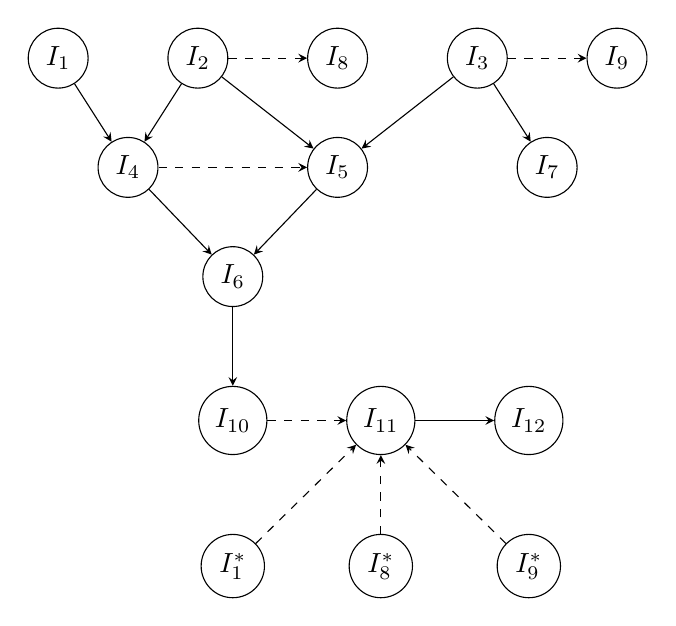
\begin{tikzpicture}[node distance=1cm, >=stealth]
            % Nodes
            \node[circle, draw] (I1) {$I_{1}$};
            \node[circle, draw, right=of I1] (I2) {$I_{2}$};
            \node[circle, draw, right=of I2] (I8) {$I_{8}$};
            \node[circle, draw, right=of I8] (I3) {$I_{3}$};
            \node[circle, draw, right=of I3] (I9) {$I_{9}$};

            \node[circle, draw, below=1cm of $(I1)!0.5!(I2)$] (I4) {$I_{4}$};
            \node[circle, draw, below=1cm of $(I2)!0.5!(I3)$] (I5) {$I_{5}$};
            \node[circle, draw, below=1cm of $(I3)!0.5!(I9)$] (I7) {$I_{7}$};

            \node[circle, draw, below=1cm of $(I4)!0.5!(I5)$] (I6) {$I_{6}$};

            \node[circle, draw, below=of I6] (I10) {$I_{10}$};
            \node[circle, draw, right=of I10] (I11) {$I_{11}$};
            \node[circle, draw, right=of I11] (I12) {$I_{12}$};

            \node[circle, draw, below=of I10] (I1_bis) {$I_{1}^{*}$};
            \node[circle, draw, below=of I11] (I8_bis) {$I_{8}^{*}$};
            \node[circle, draw, below=of I12] (I9_bis) {$I_{9}^{*}$};


            \draw[dashed, ->] (I4) -- (I5);
            \draw[dashed, ->] (I2) -- (I8);
            \draw[dashed, ->] (I3) -- (I9);
            \draw[dashed, ->] (I10) -- (I11);
            \draw[dashed, ->] (I1_bis) -- (I11);
            \draw[dashed, ->] (I8_bis) -- (I11);
            \draw[dashed, ->] (I9_bis) -- (I11);

            \draw[->] (I1) -- (I4);
            \draw[->] (I2) -- (I4);
            \draw[->] (I2) -- (I5);
            \draw[->] (I3) -- (I5);
            \draw[->] (I3) -- (I7);
            \draw[->] (I4) -- (I6);
            \draw[->] (I5) -- (I6);
            \draw[->] (I6) -- (I10);
            \draw[->] (I11) -- (I12);
        \end{tikzpicture}
    \end{center}
    An oriented line indicates a RAW dependency. A dashed line indicates a WAR or WAW dependency. For this reason, labels are not inserted. Additionally, since the latency is calculated by hand, no text is inserted to avoid confusion in the graph. The asterisk indicates that these nodes were redrawn for readability.
\end{examplebox}

\begin{flushleft}
    \textcolor{Green3}{\faIcon{question-circle} \textbf{What is the Critical Path?}}
\end{flushleft}
The \definition{Critical Path} is the \textbf{longest path} through the dependence graph, starting from an entry instruction and ending at an instruction with no successors.
\begin{itemize}
    \item It represents the \textbf{minimum number of clock cycles} \hl{needed to execute the basic block}, even with unlimited resources.
    \item Any attempt to \textbf{speed up execution} (through scheduling or parallelism) \textbf{cannot beat this lower bound}.
\end{itemize}
If our goal is to schedule instructions as efficiently as possible, the critical path is our \textbf{primary constraint}.
    \subsubsection{ASAP Scheduling Algorithm (As Soon As Possible)}\label{subsubsection: ASAP Scheduling Algorithm}

\definition{ASAP (As Soon As Possible) Scheduling} is a \textbf{greedy scheduling algorithm} used in instruction scheduling. Its main idea is to \textbf{schedule each operation as early as possible} once its \textbf{dependencies are satisfied}.
\begin{itemize}
    \item It \hl{does not consider resource constraints}.
    \item It focuses only on \textbf{data readiness}.
    \item It is useful for computing \textbf{lower bounds} on execution time and for \textbf{priority estimation}.
\end{itemize}

\begin{flushleft}
    \textcolor{Green3}{\faIcon{tools} \textbf{How ASAP Scheduling Works}}
\end{flushleft}
\begin{enumerate}
    \item Build the \textbf{dependence graph} (page \pageref{subsubsection: Dependence Graph and Critical Path}).
    \item Initialize a \textbf{ready list} with all \textbf{source nodes} (instructions with no predecessors). A \definition{Ready List} is a list of all instructions \textbf{ready to be scheduled} at a given cycle. An \hl{instruction is ready} if:
    \begin{itemize}
        \item All its \hl{predecessors} have been \hl{scheduled}.
        \item Its \hl{operands are available} (i.e., computed and propagated).
    \end{itemize}
    \item For each cycle:
    \begin{itemize}
        \item Schedule every instruction in the ready list.
        \item Update successors (check if all their predecessors are now scheduled).
        \item Move newly ready instructions into the next cycle's ready list.
    \end{itemize}
    \item Repeat until all instructions are scheduled.
\end{enumerate}
ASAP produces \textbf{one of the shortest possible schedules}, assuming no resource constraints. The result gives the \textbf{earliest cycle} at which each instruction can execute.

\highspace
\begin{flushleft}
    \textcolor{Green3}{\faIcon{question-circle} \textbf{Why use ASAP Scheduling if it ignores resource constraints?}}
\end{flushleft}
\begin{enumerate}
    \item \textbf{It Computes a Theoretical Lower Bound}. ASAP gives us the earliest possible execution cycle for each instruction, assuming infinite resources. The critical path of the dependence graph emerges directly from ASAP: it is the shortest possible execution time, even for a perfectly parallel machine. We use \textbf{ASAP as a baseline} because \textbf{we know we can't do better than this in terms of schedule length}.

    \item \textbf{It Helps Assign Priorities for Real Scheduling Algorithms}. In list-based scheduling, instructions are chosen from the ready list based on priority. One way to assign this priority is using the Longest Path to Sink (from ASAP): instructions deeper in the graph (closer to the end) are more urgent. So \textbf{even if ASAP isn't the final schedule, it informs how to choose wisely in realistic algorithms}.
    
    \item \textbf{It's a Building Block for More Advanced Scheduling}. Many algorithms, like List Scheduling, start by computing the ASAP schedule. Then they incorporate resource constraints and adjust from there. Think of it as the ``\textbf{first approximation}'', \textbf{later refined under constraints}.
    
    \item \textbf{Compiler Simplicity in Early Stages}. In early compiler passes (before hardware-specific optimization), ASAP can: help restructure code, estimate ILP, and guide unrolling or pipelining transformations.
\end{enumerate}
A great \hl{analogy}: ASAP is like planning a trip \textbf{assuming we hit green lights at every intersection}. It's not realistic, but it \textbf{gives us a best-case travel time}, which is useful for planning and comparison.

\begin{examplebox}[: ASAP Scheduling Algorithm]
    Consider the following dependence graph:
    \begin{center}
        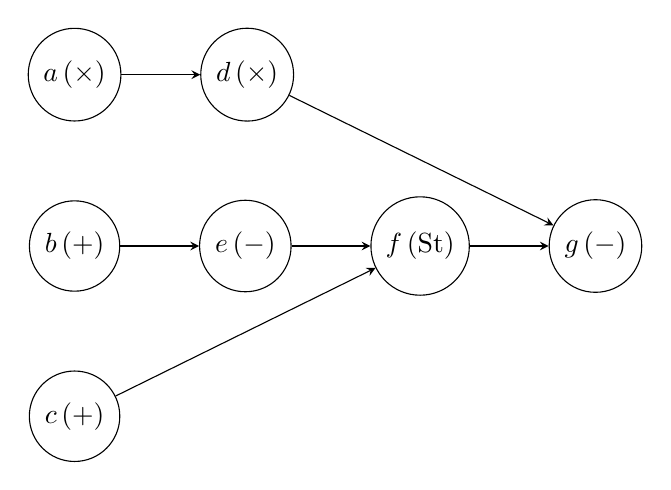
\begin{tikzpicture}[node distance=1cm, >=stealth]
            \node[circle, draw] (a) {$a \left(\times\right)$};
            \node[circle, draw, below=of a] (b) {$b \left(+\right)$};
            \node[circle, draw, below=of b] (c) {$c \left(+\right)$};

            \node[circle, draw, right=of a] (d) {$d \left(\times\right)$};
            \node[circle, draw, right=of b] (e) {$e \left(-\right)$};

            \node[circle, draw, right=of e] (f) {$f \left(\text{St}\right)$};
            
            \node[circle, draw, right=of f] (g) {$g \left(-\right)$};

            \draw[->] (a) -- (d);
            \draw[->] (b) -- (e);
            \draw[->] (c) -- (f);
            \draw[->] (e) -- (f);
            \draw[->] (d) -- (g);
            \draw[->] (f) -- (g);
        \end{tikzpicture}
    \end{center}
    Each node has the corresponding operation in brackets. For example, ``St'' is the store operation. Multiply operations take three latency cycles; ALU operations (addition and subtraction) take one; and the store operation takes two.

    \highspace
    \begin{minipage}{0.35\textwidth}
        \centering
        \begin{tabular}{@{} c | c @{}}
            \toprule
            \multicolumn{2}{c}{Ready List} \\
            \midrule
            \textbf{Cycle} & \textbf{Ready List} \\
            \midrule
            1 & $a$, $b$, $c$ \\
            2 & $e$ \\
            3 & $f$ \\
            4 & $d$ \\
            5 & \\
            6 & \\
            7 & $g$ \\
            \bottomrule
        \end{tabular}
    \end{minipage}
    \hfill
    \begin{minipage}{0.6\textwidth}
        \centering
        \begin{tabular}{@{} c | c | c | c | c @{}}
            \toprule
            \multicolumn{5}{c}{Resource Reservation Table} \\
            \midrule
            \textbf{Cycle} & \textbf{ALU1} & \textbf{ALU2} & \textbf{L/S} & \textbf{MUL} \\
            \midrule
            1 & $b$ & $c$ &     & $a$ \\
            2 & $e$ &   &     & $a$ \\
            3 & $f$ &   & $f$   & $a$ \\
            4 & &   & $f$   & $d$ \\
            5 & &   &     & $d$ \\
            6 & &   &     &   \\
            7 & $g$ &   &     &   \\
            \bottomrule
        \end{tabular}
    \end{minipage}
\end{examplebox}
    \subsubsection{List-Based Scheduling Algorithm}

The \definition{List-Based Scheduling Algorithm} is a realistic and practical scheduling technique that improves over ASAP by taking into account \textbf{resource constraints}.

\highspace
Unlike ASAP (which assumes infinite resources), \textbf{list-based scheduling}:
\begin{itemize}
    \item Works with a limited number of functional units (ALU, MUL, etc.).
    \item Ensures that at each cycle:
    \begin{itemize}[label=\textcolor{Green3}{\faIcon{check}}]
        \item We \textbf{do not oversubscribe} any hardware unit.
        \item We only schedule instructions \textbf{whose operands are ready}.
    \end{itemize}
\end{itemize}
This reflects \textbf{real hardware limitations} in VLIW superscalar, or statically scheduled pipelined processors.

\highspace
\begin{flushleft}
    \textcolor{Green3}{\faIcon{tools} \textbf{Algorithm Steps}}
\end{flushleft}
At each cycle, the algorithm maintains a \definition{Ready Set}, similar to ASAP. But now, when multiple instructions are ready, and \textbf{not all can be scheduled} in parallel, it must \textbf{choose} based on a \textbf{priority}.
\begin{enumerate}
    \item Build the dependence graph.
    \item Compute \textbf{priorities} for all nodes (typically with longest-path-to-sink). Nodes closer to the end of the graph are \textbf{more critical} (less slack). The compiler calculates for each instruction:
    \begin{equation*}
        \text{priority}\left(i\right) = \text{Max path length from } i \text{ to a sink node}
    \end{equation*}
    Higher priority, more urgent to schedule.
    \item Initialize the \textbf{Ready Set} with nodes that have no predecessors.
    \item For each cycle:
    \begin{itemize}
        \item While resources are available and Ready Set is not empty:
        \begin{itemize}
            \item Pick the \textbf{highest-priority instruction} that fits into available resources.
            \item Assign it to the current cycle.
            \item Mark it as scheduled
        \end{itemize}
        \item Update the Ready Set: add successors whose dependencies are now satisfied.
    \end{itemize}
    \item Repeat until all instructions are scheduled.
\end{enumerate}

\newpage

\begin{examplebox}[: List-Based Scheduling Algorithm]
    Consider the following dependence graph:
    \begin{center}
        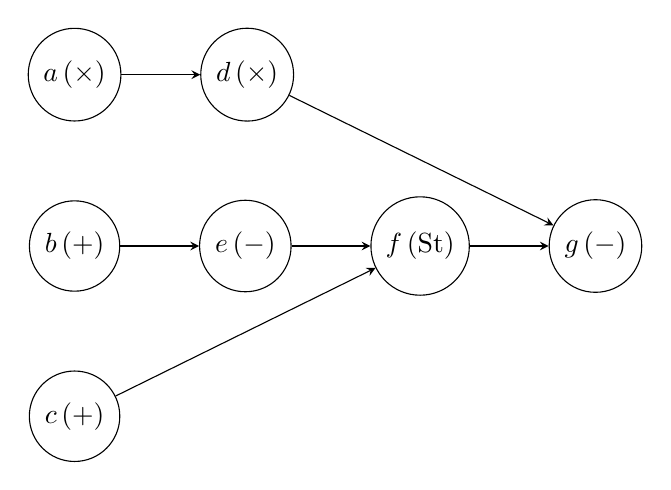
\begin{tikzpicture}[node distance=1cm, >=stealth]
            \node[circle, draw] (a) {$a \left(\times\right)$};
            \node[circle, draw, below=of a] (b) {$b \left(+\right)$};
            \node[circle, draw, below=of b] (c) {$c \left(+\right)$};

            \node[circle, draw, right=of a] (d) {$d \left(\times\right)$};
            \node[circle, draw, right=of b] (e) {$e \left(-\right)$};

            \node[circle, draw, right=of e] (f) {$f \left(\text{St}\right)$};
            
            \node[circle, draw, right=of f] (g) {$g \left(-\right)$};

            \draw[->] (a) -- (d);
            \draw[->] (b) -- (e);
            \draw[->] (c) -- (f);
            \draw[->] (e) -- (f);
            \draw[->] (d) -- (g);
            \draw[->] (f) -- (g);
        \end{tikzpicture}
    \end{center}
    Each node has the corresponding operation in brackets. For example, ``St'' is the store operation. Multiply operations take three latency cycles; ALU operations (addition and subtraction) take one; and the store operation takes two.

    \highspace
    \begin{minipage}{0.35\textwidth}
        \centering
        \begin{tabular}{@{} c | c @{}}
            \toprule
            \multicolumn{2}{c}{Ready List} \\
            \midrule
            \textbf{Cycle} & \textbf{Ready List} \\
            \midrule
            1 & $a$, $b$, $c$ \\
            2 & $c$, $e$ \\
            3 & $e$ \\
            4 & $d$, $f$ \\
            5 & \\
            6 & \\
            7 & $g$ \\
            \bottomrule
        \end{tabular}
    \end{minipage}
    \hfill
    \begin{minipage}{0.6\textwidth}
        \centering
        \begin{tabular}{@{} c | c | c | c | c @{}}
            \toprule
            \multicolumn{5}{c}{Resource Reservation Table} \\
            \midrule
            \textbf{Cycle} & \textbf{ALU1} & \textbf{L/S} & \textbf{MUL} \\
            \midrule
            1 & $b$ &       & $a$   \\
            2 & $c$ &       & $a$   \\
            3 & $e$ & $f$   & $a$   \\
            4 &     & $f$   & $d$   \\
            5 &     &       & $d$   \\
            6 &     &       & $d$   \\
            7 & $g$ &       &       \\
            \bottomrule
        \end{tabular}
    \end{minipage}

    \begin{center}
        \begin{tabular}{@{} c | c | c | c @{}}
            \toprule
            \multicolumn{4}{c}{VLIW Code} \\
            \midrule
            \textbf{Cycle} & \textbf{ALU1} & \textbf{L/S} & \textbf{MUL} \\
            \midrule
            1 & $b$   &   & $a$ \\
            2 & $c$   &   &   \\
            3 & $e$   &   &   \\
            4 &     & $f$ & $d$ \\
            5 &     &   &   \\
            6 &     &   &   \\
            7 & $g$   &   &   \\
            \bottomrule
        \end{tabular}
    \end{center}
\end{examplebox}
    \subsubsection{Local vs Global Scheduling}

In modern compilers, especially for statically scheduled architectures like VLIW, \textbf{instruction scheduling can be applied at two levels}:
\begin{itemize}
    \item \important{Local Scheduling: Within Basic Blocks}. \textbf{Local scheduling} operates \textbf{inside a single basic block}, where:
    \begin{itemize}
        \item The control flow is \textbf{linear} (no internal branches).
        \item The compiler has \textbf{full knowledge} of all instructions and dependencies.
    \end{itemize}
    \textcolor{Green3}{\faIcon{bullseye}} The \textcolor{Green3}{\textbf{objective}} is to:
    \begin{itemize}
        \item Maximize instruction-level parallelism (ILP).
        \item Minimize execution time of each block.
        \item Efficiently fill VLIW slots with real instructions (reduce NOPs).
    \end{itemize}
    \textcolor{Green3}{\faIcon{tools} \textbf{Techniques}}
    \begin{itemize}
        \item ASAP scheduling (page \pageref{subsubsection: ASAP Scheduling Algorithm}).
        \item List-based scheduling (page \pageref{subsubsection: List-Based Scheduling Algorithm}).
        \item Loop unrolling (page \pageref{paragraph: Loop Unrolling}).
        \item Software pipelining.
    \end{itemize}
    Local scheduling is \textbf{simpler} and \textbf{effective}, but limited:
    \begin{itemize}[label=\textcolor{Red2}{\faIcon{times}}]
        \item It \textbf{cannot move instructions} across block boundaries.
        \item \textbf{ILP is bounded} by the size and dependencies of the block.
    \end{itemize}


    \item \important{Global Scheduling: Across Basic Blocks}. \textbf{Global Scheduling} considers a \textbf{wider scope}, across \textbf{multiple basic blocks}, \hl{allowing reordering of instructions}:
    \begin{itemize}
        \item Across \textbf{branches}.
        \item Across \textbf{loop boundaries}.
        \item Even across \textbf{entire control paths}.
    \end{itemize}
    \textcolor{Green3}{\faIcon{bullseye}} The \textcolor{Green3}{\textbf{goal}} is to:
    \begin{itemize}
        \item Exploit \textbf{more ILP than local scheduling} allows.
        \item Hide or overlap long-latency operations.
        \item Restructure code for better pipeline utilization.
    \end{itemize}
    \textcolor{Red2}{\faIcon{ban} \textbf{Challenges}}
    \begin{itemize}
        \item Must preserve \textbf{control and data dependences}.
        \item Must generate \textbf{compensation code} to fix incorrect speculative\break moves.
        \item More \textbf{complex} and \textbf{expensive} to implement in the compiler.
    \end{itemize}
\end{itemize}

\begin{table}[!htp]
    \centering
    \begin{tabular}{@{} l l p{17em} @{}}
        \toprule
        Technique & Type & Description \\
        \midrule
        \textbf{Loop Unrolling}         & Local     & Replicates loop body to increase basic block size and expose ILP.     \\ [.5em]
        \textbf{Software Pipelining}    & Local     & Reorganizes instructions from different iterations to overlap them.   \\ [.5em]
        \textbf{Trace Scheduling}       & Global    & Predicts a frequent path (trace) and aggressively schedules it.       \\ [.5em]
        \textbf{Superblock Scheduling}  & Global    & Extension of trace scheduling; allows multiple exits, single entry.   \\
        \bottomrule
    \end{tabular}
    \caption{Techniques Overview.}
\end{table}
    \subsubsection{Local Scheduling Techniques}

\paragraph{Loop Unrolling}\label{paragraph: Loop Unrolling}

\definition{Loop Unrolling} is a \textbf{compiler optimization} that duplicates the \textbf{body of a loop multiple times}, reducing the number of loop control instructions and exposing \textbf{more parallelism} within the loop body.

\highspace
\begin{flushleft}
    \textcolor{Green3}{\faIcon{question-circle} \textbf{What is the goal?}}
\end{flushleft}
\begin{itemize}
    \item To \textbf{increase the size of the basic block} inside a loop.
    \item To \textbf{expose more independent instructions} to the scheduler.
    \item To \textbf{reduce the number of branches and loop counters}, lowering control.
\end{itemize}

\begin{flushleft}
    \textcolor{Green3}{\faIcon{check-circle} \textbf{Benefits}}
\end{flushleft}
\begin{enumerate}
    \item \textbf{More instruction-level parallelism (ILP)}, more instructions can be scheduled in parallel.
    \item \textbf{Reduced loop overhead}, fewer \texttt{BNE}, \texttt{SUBI}, etc., executed per iteration.
    \item \textbf{Better resource utilization}, more functional units are kept busy (fewer NOPs).
\end{enumerate}

\begin{flushleft}
    \textcolor{Red2}{\faIcon{times-circle} \textbf{Downsides}}
\end{flushleft}
\begin{enumerate}
    \item \textbf{Increased register pressure}, more temporary values, so more registers needed.
    \item \textbf{Increased code size}, can lead to \textbf{instruction cache misses}.
\end{enumerate}

\highspace
\begin{examplebox}[: No Unrolling vs. Loop Unrolling]
    Consider the following code:
    \begin{lstlisting}[language=C]
for (i=1000; i>0; i--)
    x[i] = x[i] + s;
    \end{lstlisting}
    \begin{itemize}
        \item No Unrolling, one iteration in Assembly:
        \begin{lstlisting}[language=riscv]
Loop: LD    F0, 0(R1)
      ADD   F4, F0, F2
      SD    F4, 0(R1)
      SUBI  R1, R1, 8
      BNE   R1, R2, Loop\end{lstlisting}
        \begin{itemize}
            \item Execution time: \textbf{10 cycles per iteration}
            \item Efficiency: 5 instructions, 10 cycles, then \textbf{50\%} ($\text{IPC} = 0.5$)
        \end{itemize}

        \newpage

        \item $4\times$ Loop Unrolling (not yet optimized):
        \begin{lstlisting}[language=riscv]
Loop: LD  F0,   0(R1)
      ADD F4,   F0, F2
      SD  F4,   0(R1)

      LD  F0,  -8(R1)
      ADD F4,  F0, F2
      SD  F4,  -8(R1)

      LD  F0, -16(R1)
      ADD F4,  F0, F2
      SD  F4, -16(R1)

      LD  F0, -24(R1)
      ADD F4,  F0, F2
      SD  F4, -24(R1)

      SUBI R1, R1, 32
      BNE  R1, R2, Loop\end{lstlisting}
        Only \textbf{true dependences} remain between \texttt{SUBI} and \texttt{BNE}. But there's a problem: we are \textbf{reusing \texttt{F0}, \texttt{F4}}, and leads to \textbf{WAW and WAR hazards}.
    \end{itemize}
\end{examplebox}

\begin{flushleft}
    \textcolor{Green3}{\faIcon{check-circle} \textbf{Register Renaming to Resolve Name Dependencies}}
\end{flushleft}
As we saw in the previous example, there are WAW and WAR hazards due to the use of the same register during loop unrolling. To remove false dependencies (WAW and WAR), the compiler performs \textbf{register renaming}:
\begin{lstlisting}[language=riscv]
Loop: LD   F0,   0(R1)
      ADD  F4,   F0, F2
      SD   F4,   0(R1)

      LD   F6,  -8(R1)
      ADD  F8,  F6, F2
      SD   F8,  -8(R1)

      LD   F10, -16(R1)
      ADD  F12, F10, F2
      SD   F12, -16(R1)

      LD   F14, -24(R1)
      ADD  F16, F14, F2
      SD   F16, -24(R1)

      SUBI R1, R1, 32
      BNE  R1, R2, Loop
\end{lstlisting}
Now all instructions use \textbf{unique registers}, and only \textbf{true dependencies remain}. It allows \textbf{maximum scheduling freedom}.
\begin{itemize}
    \item \textbf{Execution time}: 16 cycles per 4 iterations, then 4 cycles per iteration.
    \item \textbf{Loop overhead}: 4 cycles per 4 iterations, then 1 cycle per iteration.
    \item \textbf{Efficiency}: 14 instructions, 16 cycles, then $14 \div 16 = 87.5\%$
\end{itemize}

\highspace
\textcolor{Green3}{\faIcon{\speedIcon} \textbf{Effect on ILP}} After renaming, instructions are independent and can be \textbf{reordered or scheduled in parallel}:
\begin{itemize}
    \item Original loop: 1 useful instruction per cycle.
    \item After unrolling and renaming: up to 4 useful instructions per cycle (in theory)
\end{itemize}
This enables \textbf{better pipelining}, \textbf{more efficient use of wide VLIW issue slots}, and \textbf{less stalling}.

\begin{table}[!htp]
    \centering
    \begin{tabular}{@{} l p{25em} @{}}
        \toprule
        Concept & Description \\
        \midrule
        Loop unrolling    & Duplicates loop body to expose more ILP.                                 \\ [.3em]
        Benefit           & Reduces loop overhead, increases block size.                             \\ [.3em]
        Drawback          & Increases register pressure and code size.                               \\ [.3em]
        Register renaming & Eliminates name dependencies (WAW/WAR) to enable parallel scheduling.    \\ [.3em]
        Result            & More efficient and parallel scheduling possible.                         \\
        \bottomrule
    \end{tabular}
\end{table}

\begin{flushleft}
    \textcolor{Green3}{\faIcon{\speedIcon} \textbf{Performance Metrics of Unrolling}}
\end{flushleft}
When applying \textbf{loop unrolling}, the goal is not just to make the code longer, it's to \textbf{execute faster}. We can measure this improvement through several performance metrics:
\begin{itemize}
    \item \definition{Execution Time}. The total \textbf{execution time per loop iteration} reflects how efficiently the instructions are executed.
    \begin{itemize}
        \item Execution time \textbf{includes} useful operations \textbf{plus stalls/NOPs}.
        \item Lower execution time $=$ better use of ILP and scheduling.
    \end{itemize}
    We typically express it as:
    \begin{equation}
        \text{Execution time} = \dfrac{\text{Cycles to execute unrolled loop}}{\text{Number of iterations covered}}
    \end{equation}


    \item \definition{Loop Overhead}. Loop overhead includes \textbf{instructions that are not part of the loop's core computation}:
    \begin{itemize}
        \item \texttt{SUBI} (loop counter update).
        \item \texttt{BNE} (branch).
        \item Any \texttt{NOP} needed to avoid hazards.
    \end{itemize}
    \hl{Reducing overhead}:
    \begin{itemize}
        \item Makes more room for \textbf{useful instructions}.
        \item Boosts \textbf{efficiency}.
    \end{itemize}
    In unrolling we do $4\times$ the work \textbf{but only 1 loop update}, loop overhead is \textbf{amortized} over more iterations.


    \item \definition{Code Efficiency}. Code efficiency \textbf{quantifies how well instruction slots are used}. Defined as:
    \begin{equation}
        \text{Efficiency} = \dfrac{\text{Number of useful operations}}{\text{Total number of instruction slots}}
    \end{equation}
    This tells us \textbf{how many issue slots are actually contributing to the computation}.
\end{itemize}
    \paragraph{Software Pipelining}\label{paragraph: Software Pipelining}

\definition{Software Pipelining} is a scheduling technique where instructions from \textbf{different iterations} of a loop are \textbf{reordered and overlapped} to keep functional units busy every cycle.

\highspace
Instead of executing one full iteration at a time, the processor \textbf{starts a new iteration every cycle}, with different stages of previous iterations still in progress, similar to hardware pipelining.

\highspace
\begin{flushleft}
    \textcolor{Green3}{\faIcon{balance-scale} \textbf{Comparison with Loop Unrolling}}
\end{flushleft}
\begin{table}[!htp]
    \centering
    \begin{tabular}{@{} l p{11em} p{12em} @{}}
        \toprule
        \textbf{Aspect} & \textbf{Loop Unrolling} & \textbf{Software Pipelining} \\
        \midrule
        \textbf{Structure}          & Duplicates code                               & Keeps loop body same size                     \\ [.5em]
        \textbf{ILP exposure}       & Gained by replicating loop body               & Gained by reordering across iterations        \\ [.5em]
        \textbf{Code size}          & Increases (proportional to unrolling factor)  & Remains compact                               \\ [1.8em]
        \textbf{Scheduling scope}   & Within a block                                & Across multiple iterations                    \\ [.5em]
        \textbf{Register pressure}  & High (due to duplication)                     & Very high (many live temporaries)             \\ [.5em]
        \textbf{Throughput}         & Good (bounded by unrolling factor)            & Potentially optimal (1 iteration per cycle)   \\
        \bottomrule
    \end{tabular}
    \caption{Comparison with Loop Unrolling.}
\end{table}

\begin{flushleft}
    \textcolor{Green3}{\faIcon{stream} \textbf{Phases of Software Pipelined Loop}}
\end{flushleft}
A software-pipelined loop executes in \textbf{three distinct phases}:
\begin{enumerate}
    \item \important{Startup (Prologue)}. Initial cycles where instructions from the \textbf{first few iterations} begin execution. Not all stages are filled yet.
    
    \item \important{Steady State}. The \textbf{core phase}: every cycle completes one iteration, while other iterations are in progress. This is where \textbf{ILP is fully exploited}.
    
    \item \important{Drain (Epilogue)}. Final cycles where instructions from the \textbf{last few iterations} finish. No new iterations start; pipeline ``drains'' out.
\end{enumerate}

\newpage

\begin{table}[!htp]
    \centering
    \begin{tabular}{@{} l p{22em} @{}}
        \toprule
        Concept & Description \\
        \midrule
        \textbf{Software pipelining} & Reorders loop instructions from different iterations.            \\ [.3em]
        \textbf{Objective}           & Maximize ILP by filling the execution pipeline every cycle.      \\ [.3em]
        \textbf{Benefits}            & Compact code, steady throughput, ideal for VLIW.                 \\ [.3em]
        \textbf{Trade-offs}          & High register pressure, scheduling complexity.                   \\ [.3em]
        \textbf{Execution phases}    & Startup (filling), Steady (full overlap), Drain (finishing up).  \\
        \bottomrule
    \end{tabular}
\end{table}

\begin{examplebox}[: Software Pipelining]
    We start with the original scalar loop:
    \begin{lstlisting}[language=riscv]
Loop: LD    F0, 0(R1)
      ADD   F4, F0, F2
      SD    F4, 0(R1)
      SUBI  R1, R1, 8
      BNE   R1, R2, Loop\end{lstlisting}
    \begin{enumerate}
        \item Loads a value from memory.
        \item Adds a scalar value \texttt{F2}.
        \item Stores it back.
        \item Updates the pointer.
        \item Branches if not done.
    \end{enumerate}
    \textbf{Execution time} per iteration: 5-6 cycles. So only \textbf{one useful result per loop iteration}, poor ILP.

    \highspace
    To apply software pipelining, we \textbf{reorder instructions} from \textbf{different iterations} to \textbf{fill functional units}. Assume all dependencies are respected (RAW), and rename registers to avoid WAR/WAW hazards.
    \begin{lstlisting}[language=riscv]
LD    F0, 0(R1)      # I0
ADD   F4, F0, F2     # I1 from previous iteration
SD    F4, -8(R1)     # I2 from 2 iterations ago\end{lstlisting}
    This version performs \texttt{LD} \textbf{for current iteration}, \texttt{ADD} \textbf{for previous}, \texttt{SD} \textbf{for 2 iterations ago}. This matches the \textbf{steady state} of a pipelined execution: \textbf{each cycle does useful work from 3 iterations simultaneously}. We now issue \textbf{one full result per cycle} after startup.

    \highspace
    Now let's handle address computation correctly. Assume:
    \begin{itemize}
        \item \texttt{R1} points to current element.
        \item We track offset correctly for each instruction.
    \end{itemize}
    \begin{lstlisting}[language=riscv]
# Prologue (Startup)
LD    F0, 0(R1)

# Loop body (Steady state)
Loop: LD    F6, -8(R1)       # LD for next iteration
      ADD   F4, F0, F2       # ADD from previous iteration
      SD    F4, 0(R1)        # SD from 2 iterations ago
      SUBI  R1, R1, 8
      BNE   R1, R2, Loop
      MOV   F0, F6           # prepare F0 for next ADD\end{lstlisting}
    \begin{center}
        \begin{tabular}{@{} l l @{}}
            \toprule
            Operation & From Iteration \\
            \midrule
            \texttt{LD F6}  & \texttt{i + 1} \\ [.3em]
            \texttt{ADD F4} & \texttt{i}     \\ [.3em]
            \texttt{SD F4}  & \texttt{i - 1} \\
            \bottomrule
        \end{tabular}
    \end{center}
    \begin{itemize}
        \item \texttt{F0} is shifted forward via \texttt{MOV}.
        \item Pipelined stages are handled via register flow.
        \item Control remains simple, and code is compact.
    \end{itemize}
    \begin{center}
        \begin{adjustbox}{width={\textwidth},totalheight={\textheight},keepaspectratio}
            \begin{tabular}{@{} l l l @{}}
                \toprule
                Version & Throughput & Notes \\
                \midrule
                Classic Loop        & 1 result every 5 cycles       & Poor resource utilization. \\ [.3em]
                Pipelined (steady)  & \textbf{1 result per cycle}   & Maximized ILP. \\ [.3em]
                Code size           & Small (no unrolling)          & More compact than unrolling. \\
                \bottomrule
            \end{tabular}
        \end{adjustbox}
    \end{center}
\end{examplebox}
    \subsubsection{Global Scheduling}

\paragraph{Trace Scheduling}\label{paragraph: Trace Scheduling}

\definition{Trace Scheduling} is a \textbf{global instruction scheduling technique} that aims to optimize the \textbf{most frequently executed paths} (called \textbf{traces}) through a program's control flow graph (CFG).

\highspace
It allows the compiler to move instructions \textbf{across basic block boundaries}, including across branches, to expose more \textbf{instruction-level parallelism (ILP)} and fill wide VLIW instruction words more efficiently.
\begin{itemize}
    \item \textbf{Step 1:} \definition{Trace Selection}. A \textbf{trace} is a likely path through the code, a \textbf{linear sequence of basic blocks} that are expected to execute one after the other \textbf{most of the time}.
    \begin{flushleft}
        \textcolor{Green3}{\faIcon{question-circle} \textbf{How traces are selected}}
    \end{flushleft}
    \begin{itemize}
        \item Based on \textbf{profiling information}, static heuristics, or feedback from runs.
        \item Hot paths (e.g., common branches of \texttt{if}-\texttt{else} or main loop bodies) are prioritized.
        \item A trace may include: \textbf{forward branches}, \textbf{backward branches}, multiple blocks treated as a \textbf{single scheduling unit}.
    \end{itemize}
    We can think of a trace as a \textbf{``super-block'' of code} that is optimized as a single unit, assuming that it is frequently executed in that order.


    \item \textbf{Step 2:} \definition{Trace Compaction (Scheduling)}. Once the trace is selected, the compiler:
    \begin{itemize}
        \item Builds a \textbf{dependence graph} for the entire trace.
        \item Applies \textbf{list-based scheduling} across all blocks in the trace.
        \item Moves instructions \textbf{upward} across branches if possible, to fill unused slots (VLIW-friendly).
    \end{itemize}
    This reordering allows:
    \begin{itemize}[label=\textcolor{Green3}{\faIcon{check}}]
        \item Filling of issue slots across multiple basic blocks.
        \item Earlier execution of long-latency operations (e.g., memory loads).
    \end{itemize}
\end{itemize}

\highspace
\begin{flushleft}
    \textcolor{Red2}{\faIcon{exclamation-triangle} \textbf{Speculation and Compensation Code}}
\end{flushleft}
\textcolor{Red2}{\faIcon{times-circle} \textbf{Problem.}} When instructions are \textbf{moved across branches}, they might be executed \textbf{in paths where they shouldn't}. This is called \definition{Specualtive Execution}:
\begin{itemize}
    \item The compiler \textbf{speculates} that a certain path is taken.
    \item It moves instructions \textbf{before a branch}, even if they are only \textbf{valid in one branch}.
\end{itemize}
\textcolor{Green3}{\faIcon{check-circle} \textbf{Solution: Compensation Code.}} To \textbf{preserve correctness}, the compiler adds \textbf{compensation code} in \textbf{off-trace blocks} to:
\begin{itemize}
    \item Recompute or restore the correct values.
    \item Prevent side effects (e.g., stores) from speculates
\end{itemize}

\highspace
\begin{definitionbox}[: Compensation Code]
    \definition{Compensation Code} is \textbf{extra code inserted by the compiler} to \textbf{preserve program correctness} after performing speculative instruction movement during global scheduling (e.g., in trace scheduling).
\end{definitionbox}

\highspace
\begin{examplebox}[: Compensation Code]
    Suppose this trace is selected:
    \begin{lstlisting}[language=c]
if (x > 0)
    A = B + C;  // part of the trace
else
    A = D + E\end{lstlisting}
    Compiler speculatively moves \texttt{A = B + C} above the \texttt{if}. Then in the \texttt{else} block, it inserts:
    \begin{lstlisting}[language=c]
A = D + E;      // compensation code\end{lstlisting}
    This ensures correctness \textbf{if the speculation fails}.
\end{examplebox}

\begin{table}[!htp]
    \centering
    \begin{tabular}{@{} l p{23em} @{}}
        \toprule
        Step & Action \\
        \midrule
        \textbf{Trace Selection}    & Choose most likely sequence of basic blocks (the ``hot path'').   \\ [.5em]
        \textbf{Trace Compaction}   & Reorder instructions across blocks to improve ILP and scheduling. \\ [.5em]
        \textbf{Speculation}        & Move instructions before branches, assuming likely path.          \\ [.5em]
        \textbf{Compensation Code}  & Inserted to preserve semantics if speculation was wrong.          \\
        \bottomrule
    \end{tabular}
    \caption{Trace Scheduling summary.}
\end{table}
    \paragraph{Superblock Scheduling}

\definition{Superblock Scheduling} is an evolution of \textbf{Trace Scheduling}, designed to simplify speculation management while still providing \textbf{high ILP} for \textbf{VLIW} or statically scheduled superscalar processors.

\highspace
It is a \textbf{global instruction scheduling technique} that extends Trace Scheduling, with two key design changes:
\begin{enumerate}
    \item It restricts code regions to have \textbf{only one entry point}.
    \item It allows \textbf{multiple exits}.
\end{enumerate}
This enables the compiler to \textbf{aggressively schedule instructions across basic blocks}, including across branches, but with \textbf{simpler and safer control-flow management} than full trace scheduling.

\highspace
\begin{flushleft}
    \textcolor{Green3}{\faIcon{balance-scale} \textbf{Superblocks vs Traces}}
\end{flushleft}
\begin{table}[!htp]
    \centering
    \begin{tabular}{@{} l p{11em} p{11em} @{}}
        \toprule
        Feature & \textbf{Trace} Scheduling & \textbf{Superblock} Scheduling \\
        \midrule
        Entry points        & Multiple (any predecessor block).         & \textbf{Single entry point} (one predecessor).            \\ [.5em]
        Exit points         & Multiple.                                 & Multiple.                                                 \\ [.5em]
        Control flow        & General, complex.                         & \textbf{Simplified, controlled}.                          \\ [.5em]
        Speculation         & Really aggressive, harder to manage.             & More manageable.                                          \\ [.5em]
        Compensation code   & May be needed on both sides of branches.  & Needed only on \textbf{one side} (outside the superblock).\\
        \bottomrule
    \end{tabular}
\end{table}

\highspace
\begin{flushleft}
    \textcolor{Green3}{\faIcon{question-circle} \textbf{Why is this useful?}}
\end{flushleft}
In trace scheduling, we may have \textbf{multiple entry points} into the trace, which means any speculative movement of instructions must be \textbf{repaired in many paths} (with compensation code). In \hl{Superblock Scheduling}, by \textbf{enforcing a single-entry rule}, and using \textbf{tail duplication} to eliminate side entries, the compiler can:
\begin{itemize}[label=\textcolor{Green3}{\faIcon{check}}]
    \item Speculate more \textbf{safely}.
    \item Insert \textbf{fewer compensation instructions}.
    \item Retain most of the \textbf{performance benefit} of traces.
    \item Keep control flow \textbf{more manageable}.
\end{itemize}

\newpage

\begin{flushleft}
    \textcolor{Green3}{\faIcon{tools} \textbf{Typical Structure of a Superblock}}
\end{flushleft}
A \textbf{superblock} is a \textbf{linear sequence of basic blocks} that:
\begin{itemize}
    \item Starts from a \textbf{unique entry point}.
    \item Ends at \textbf{multiple potential exists}.
    \item Is built around a \textbf{frequently executed path} (like a hot loop body or branch).
    \begin{flushleft}
        \textcolor{Green3}{\faIcon{question-circle} \textbf{How is it built?}}
    \end{flushleft}
    \begin{enumerate}
        \item \textbf{Profiling} (or prediction) selects a hot path.
        \item \definition{Tail Duplication} is applied to remove alternative entries. Compiler \textbf{duplicates the tails} (exit blocks) of a region, because this ensures all control flow into the superblock happens from \textbf{a single point}.
        \item The resulting region becomes a \textbf{superblock} (safe to schedule aggressively).
    \end{enumerate}
\end{itemize}
We can think of it as a \textbf{safer, more controlled trace}, scheduled to maximize instruction-level parallelism (ILP) on VLIW or superscalar machines.

\highspace
\begin{examplebox}[: Superblock]
    Original code:
    \begin{lstlisting}[language=c]
if (x > 0)
    A = B + C;
else
    A = D + E;\end{lstlisting}
    We want to \textbf{schedule more instructions in parallel}. But the compiler sees a branch:
    \begin{itemize}
        \item In one path: \texttt{A = B + C}
        \item In the other: \texttt{A = D + E}
    \end{itemize}
    To do \textbf{Superblock Scheduling}, we assume that \textbf{the first path} (\texttt{x > 0}) \textbf{is more frequent} (we get this from profiling).

    \begin{enumerate}
        \item We take the \textbf{most frequent path} (\texttt{x > 0}).
        \item We include its block: \texttt{A = B + C}.
        \item We move it \textbf{before the branch}, so it's scheduled early (speculative move).
        \item We make the region a \textbf{superblock}: a linear code region with one entry.
        \begin{lstlisting}[language=c]
A = B + C         // speculated! Scheduled early
if (x <= 0)
    A = D + E     // compensation code\end{lstlisting}
    \end{enumerate}
    Now:
    \begin{itemize}
        \item If the branch is \emph{not taken} (\texttt{x > 0}), then \texttt{A = B + C} is correct.
        \item If the branch \emph{is taken} (\texttt{x $\le$ 0}), then we \textbf{fix \texttt{A}} using compensation code.
    \end{itemize}
    It is called a ``superblock'' because we treat that piece of code as one large block when scheduling. The compiler: optimizes this region together, tries to issue as many instructions per cycle as possible, and assumes most of the time the ``hot path'' will be followed.
\end{examplebox}

    %%%%%%%%%%%%%%%%%%%
    % Advanced Memory %
    %%%%%%%%%%%%%%%%%%%
    \section{VLIW (Very Long Instruction Word)}

\subsection{Introduction}

Traditional \textbf{compilers} use \textbf{static code scheduling} to exploit Instruction-Level Parallelism (ILP). Key tasks of the compiler:
\begin{itemize}
    \item  Detect \textbf{parallelizable} instructions considering: Hardware resource constraints and Data dependencies.
    \item \textbf{Schedule} instructions to execute \textbf{in parallel} when possible.
    \item Otherwise, \textbf{insert \texttt{NOP}s} (No Operations) if no safe parallel execution is possible.
\end{itemize}
Statically scheduled processors trust the compiler to ``fill the pipeline'' and avoid hazards at compile time.

\highspace
\begin{flushleft}
    \textcolor{Green3}{\faIcon{book} \textbf{VLIW Processors: Alternative Way to Extract ILP}}
\end{flushleft}
\definition{VLIW (Very Long Instruction Word)} \textbf{processors} are a class of architectures designed to \textbf{execute multiple operations in parallel during a single clock cycle}, but unlike superscalar processors, they \textbf{rely on the compiler} rather than on dynamic hardware mechanisms \textbf{to detect and schedule parallelism}.

\highspace
The fundamental idea behind VLIW is to \textbf{group several independent operations together into a single long instruction word}, called a \hl{bundle}. This bundle is \textbf{composed of several fixed slots}, each one \textbf{corresponding to a different functional unit in the processor}, such as an integer ALU, a floating-point unit, a load/store unit, or a branch unit.

\highspace
For example, in a 5-issue VLIW processor, a single bundle would typically carry up to five operations: integer, floating-point, load/store, branch, etc.

\highspace
The \textbf{key difference} compared \textbf{to traditional superscalar} processors lies in who decides what can run in parallel. In superscalar designs, the hardware dynamically analyzes dependencies between instructions at runtime, which requires complex circuitry for hazard detection and scheduling. In VLIW architectures, this \hl{analysis is performed entirely at compile time}. The \textbf{compiler is responsible for}:
\begin{itemize}
    \item \textbf{Statically identify} independent operations.
    \item \textbf{Solve structural hazards} (e.g., two operations trying to use the same hardware unit).
    \item \textbf{Solve data hazards} (dependencies between instructions).
    \item Insert \textbf{NOPs} when necessary.
\end{itemize}
When no useful instruction is available for a particular slot, the compiler inserts a \texttt{NOP} (no-operation). In cases where conflicts cannot be avoided, NOPs are inserted into the bundle to fill empty slots.

\highspace
\begin{flushleft}
    \textcolor{Green3}{\faIcon{question-circle} \textbf{Why move to Compiler?}}
\end{flushleft}
The problem with Superscalar is that the hardware requires complex dynamic scheduling and dependency checking, which \textbf{costs area and power}.

\highspace
\textbf{VLIW Idea} is:
\begin{itemize}
    \item Push \textbf{complexity} to the \textbf{compiler}.
    \item \textbf{Compiler groups parallel operations} into a \textbf{single bundle}.
    \item No need for runtime dependency checking anymore.
\end{itemize}
The VLIW paradigm is characterized by the use of \textbf{very wide instruction words}, \textbf{each containing multiple independent operations} (``syllables''). A multiple-issue VLIW processor typically features specialized units for integer, floating-point, memory access, and branch instructions. For example, a 4-issue VLIW processor will have four operation slots per bundle, each connected to a different unit.

\highspace
\begin{flushleft}
    \textcolor{Green3}{\faIcon{list-ul} \textbf{Multiple-issue VLIW: Operation Latencies}}
\end{flushleft}
An important aspect in VLIW scheduling is the \textbf{management of operation latencies}. Each operation type may require a \textbf{different number of clock cycles to complete}. Integer operations, memory accesses, and floating-point computations may all have varying latencies, and these differences must be carefully considered during scheduling. The \textbf{compiler must plan the execution} so that operations complete in the correct order and without causing unnecessary stalls in the pipeline.

\highspace
In summary, \hl{VLIW architectures represent a shift of complexity from the hardware to the compiler}, aiming for more efficient and simpler processor designs while demanding sophisticated compiler techniques to fully exploit available parallelism.

\highspace
\begin{flushleft}
    \textcolor{Green3}{\faIcon{book} \textbf{Single Program Counter and Branch Management}}
\end{flushleft}
In a VLIW processor, even though multiple operations are issued simultaneously, the architecture still uses a \textbf{single program counter} to fetch instructions. Each instruction fetched corresponds to a \textbf{bundle}, which can contain multiple parallel operations.

\highspace
Importantly, within each bundle, there can be \textbf{at most one branch instruction} that affects control flow. This constraint simplifies the handling of branches, making it easier for the processor to predict and manage the program's execution path.

\newpage

\begin{flushleft}
    \textcolor{Green3}{\faIcon{book} \textbf{Shared Multi-Ported Register File}}
\end{flushleft}
Since a VLIW processor issues multiple operations in parallel, the \textbf{register file must support multiple simultaneous reads and writes}. In a typical 4-issue VLIW machine, the register file needs to have enough ports to read \textbf{eight source operands} and write \textbf{four destination results} every clock cycle.

\highspace
This requirement implies a \textbf{shared, multi-ported register file}, which is one of the non-trivial aspects of the hardware design. It ensures that all functional units can access their operands without creating bottlenecks.

\highspace
\begin{flushleft}
    \textcolor{Green3}{\faIcon{book} \textbf{Importance of Parallelism and the Use of NOPs}}
\end{flushleft}
To achieve high performance, the \textbf{compiler must ensure that the source code has enough parallelism} to fill all the available operation slots in each bundle. When \textbf{sufficient independent instructions are not available}, \textbf{NOPs are inserted} into the empty slots. This insertion preserves the fixed structure of the bundle but can lead to inefficiencies if the application does not expose enough ILP.

\highspace
\begin{flushleft}
    \textcolor{Green3}{\faIcon{book} \textbf{Pipeline Organization}}
\end{flushleft}
VLIW processors often use a \textbf{pipelined execution model} similar to traditional RISC architectures. A standard pipeline might include stages like \textbf{Instruction Fetch (IF)}, \textbf{Instruction Decode (ID)}, \textbf{Register Read (RR)}, \textbf{Execution (EX)}, and \textbf{Write Back (WB)}.

\begin{figure}[!htp]
    \centering
    \includegraphics[width=\textwidth]{img/vliw-arch.pdf}
\end{figure}

\highspace
In the previous figure, a \textbf{5-stage pipeline} is used, with each bundle passing through these stages. Each operation within a bundle proceeds independently through the functional units connected to the pipeline.

\newpage

\begin{flushleft}
    \textcolor{Green3}{\faIcon{book} \textbf{Operation Dispatch and Decode}}
\end{flushleft}
If the architecture dedicates \textbf{one functional unit per slot}, the decode stage becomes relatively simple. Each operation is directed straight to its corresponding functional unit for execution without the need for complex arbitration.

\highspace
However, if there are \textbf{more functional units than slots}, meaning there is a surplus of parallel hardware resources, the architecture must include a \textbf{dispatch network}. This network is responsible for forwarding each operation, along with its operands, to the appropriate available functional unit. In this way, the design of the dispatch system depends heavily on the organization of functional units relative to the number of issue slots defined by the instruction bundle format.

    \subsection{Principle of Locality}

\hl{Cache memories are effective because programs tend to access data and instructions in} \textbf{predictable patterns}. These patterns are captured by the \definition{Principle of Locality}:
\begin{itemize}
    \item \definition{Temporal Locality} (``\emph{Time-based reuse}''). \textbf{If a memory location is accessed, it's likely to be accessed again \emph{soon}}. So recently accessed data stays in cache, because it's likely to be accessed again.
    
    For example, repeated access to loop variables:
    \begin{lstlisting}[language=c]
for (int i = 0; i < n; ++i) {
    sum += a[i];
}\end{lstlisting}
    Or reuse of stack frames in recursive functions or instruction fetches inside tight loops.
    \begin{itemize}
        \item[\textcolor{Green3}{\faIcon{tools}}] \textcolor{Green3}{\textbf{Cache strategy.}} Keep recently accessed \textbf{blocks} in cache. Don't replace them unless absolutely necessary (see LRU in later sections).
    \end{itemize}


    \item \definition{Spatial Locality} (``\emph{Nearby reuse}''). \textbf{If a memory location is accessed, it's likely that \emph{nearby locations} will be accessed soon}. In other words, if we need \texttt{a[i]}, we'll probably also need \texttt{a[i+1]}, \texttt{a[i+2]}, etc.

    For example, sequential instruction execution, or accessing elements of an array, or scanning a matrix row by row.
    
    \begin{itemize}
        \item[\textcolor{Green3}{\faIcon{tools}}] \textcolor{Green3}{\textbf{Cache strategy.}} Fetch \textbf{entire blocks}, not single words (e.g., 64-byte lines). Use \textbf{block size $>$ 1 word} to bring adjacent memory into cache.
    \end{itemize}
\end{itemize}

\highspace
\begin{flushleft}
    \textcolor{Green3}{\faIcon{question-circle} \textbf{How Caches Exploit Locality}}
\end{flushleft}
With \definition{Cache Block} we refer to the smallest unit of data moved from main memory to cache. It is typically 32, 64 or 128 bytes. It helps bring \textbf{spatial neighbors} into the cache.

\begin{table}[!htp]
    \centering
    \begin{tabular}{@{} l l @{}}
        \toprule
        Locality Type & Cache Mechanism \\
        \midrule
        Temporal    & Keep recently accessed data in cache \\ [.3em]
        Spatial     & Fetch blocks (containing multiple nearby elements) \\
        \bottomrule
    \end{tabular}
\end{table}

\noindent
Most modern cache architectures assume that the programmer writes code that follows locality principles, which i why \textbf{compiler optimizations and programming style} matter.
    \subsection{So, what is a Cache?}

\begin{definitionbox}[: Cache]
    A \definition{Cache} is a small, fast \textbf{memory} located \textbf{close to the processor} that temporarily \textbf{stores copies of data from the main memory}, aiming to reduce the average time needed to access data and instructions.
\end{definitionbox}

\noindent
Modern memory systems are structured hierarchically:
\begin{itemize}
    \item \important{Cache (upper level)}: small, fast, but expensive (SRAM). It is very close to the CPU and stores a subset of main memory to reduce access latency.
    
    \item \important{Main memory (lower level)}: larger, slower, but cheaper (DRAM). It stores the complete working set and is accessed only if data is not found in cache.
\end{itemize}
The cache acts as a \textbf{buffer} between fast CPU and slow main memory.

\highspace
\begin{flushleft}
    \textcolor{Green3}{\faIcon{book} \textbf{Terminology}}
\end{flushleft}
\begin{itemize}
    \item \definition{Cache Block} or \definition{Cache Line}. The smallest unit of data transferred between memory and cache. It is typically 32 to 128 bytes. Since a cache is divided into multiple blocks, we use:
    \begin{equation}
        \text{Number of blocks} = \dfrac{\text{Cache size}}{\text{Block size}}
    \end{equation}
    To calculate the number of blocks in the cache.

    \begin{examplebox}
        With a 64 KB cache, and 16-byte per block:
        \begin{equation*}
            \dfrac{64 \times 1024}{16} = 4096 \,\text{blocks}
        \end{equation*}
    \end{examplebox}


    \item[\textcolor{Green3}{\faIcon{check}}] \definition{Cache Hit}. Occurs when the requested memory address is \textbf{already present in the cache}. Fast access, minimal latency.
    

    \item[\textcolor{Red2}{\faIcon{times}}] \definition{Cache Miss}. Occurs when the requested address is \textbf{no in the cache}. The block must be fetched from lower-level memory.

    \textcolor{Red2}{\faIcon{exclamation-triangle} \textbf{Consequences of a miss}}
    \begin{enumerate}
        \item \textbf{Stall} CPU.
        \item Fetch block from memory.
        \item \textbf{Write} block to cache.
        \item Retry access (which now becomes a hit).
    \end{enumerate}


    \newpage


    \item \definition{Hit Time}. It is the time to:
    \begin{enumerate}
        \item Access the cache.
        \item Determine if it's a hit.
        \item Return data (if present).
    \end{enumerate}
    It is fast, typically 1-3 CPU cycles.


    \item \definition{Miss Penalty}. It is the time to:
    \begin{enumerate}
        \item Fetch the block from main memory (or next-level cache).
        \item Update cache.
        \item Resume the CPU.
    \end{enumerate}
    Much \textbf{slower} than hit time, often 10s to 100s of cycles.


    \item \definition{Average Memory Access Time (AMAT)}
    \begin{equation}
        \text{AMAT} = \text{Hit Time} + \text{Miss Rate} \times \text{Miss Penalty}
    \end{equation}
    This is the \textbf{expected cost of accessing memory}, accounting for both hits and misses.
    \begin{examplebox}
        For example:
        \begin{itemize}
            \item Hit Time: 1 cycle.
            \item Miss Rate: 5\%.
            \item Miss Penalty: 100 cycles.
        \end{itemize}
        \begin{equation*}
            \text{AMAT} = 1 + 0.05 \times 100 = 6 \text{ cycles}
        \end{equation*}
    \end{examplebox}
\end{itemize}
    \subsection{Cache Performance Metrics}

This section is about quantifying how effective a cache is, and how to improve it. Similar topics were covered on page \pageref{subsection: Memory Hierarchy}.

\highspace
The \definition{Average Memory Access Time (AMAT)} is the average time the CPU needs to access memory, considering both hits and misses. So, when accessing memory, we either get a \textbf{hit} or a \textbf{miss}:
\begin{equation*}
    \begin{array}{rcl}
        \text{AMAT} &=& (\text{Probability of Hit}) \cdot (\text{Time if Hit}) + \\ [.3em]
        && (\text{Probability of Miss}) \cdot (\text{Time if Miss})
    \end{array}
\end{equation*}
Which is written as:
\begin{equation}
    \text{AMAT} = \text{Hit Rate} \cdot \text{Hit Time} + \text{Miss Rate} \cdot \text{Miss Time}
\end{equation}
This is the \textbf{most general formula}, where:
\begin{itemize}
    \item \textbf{Hit Rate}: fraction of memory accesses that result in a hit.
    \item \textbf{Hit Time}: time to check cache and return data on a hit.
    \item \textbf{Miss Rate}: fraction of memory accesses that result in a miss.
    \item \definition{Miss Time}: time to
    \begin{enumerate}
        \item \textbf{Check} the \textbf{cache} (same time as a \emph{Hit Time}).
        \item \textbf{Fetch} the \textbf{data from main memory} (same time as a \emph{Miss Penalty})
    \end{enumerate}
    So it is reasonable to write the Miss Time as follows:
    \begin{equation}
        \text{Miss Time} = \text{Hit Time} + \text{Miss Penalty}
    \end{equation}
\end{itemize}
However, if the Miss Time is equal to the sum of the Hit Time and the Miss Penalty, then the most general formula can be \textbf{simplified}:
\begin{equation*}
    \begin{array}{rcl}
        \text{AMAT} &=& \text{Hit Rate} \cdot \text{Hit Time} + \text{Miss Rate} \cdot \text{Miss Time} \\ [.7em]
        %
        &=& \text{Hit Rate} \cdot \text{Hit Time} + \text{Miss Rate} \, \cdot \\ [.3em]
        &&  \left(\text{Hit Time} + \text{Miss Penalty}\right) \\ [.7em]
        %
        &=& \text{Hit Rate} \cdot \text{Hit Time} + \text{Miss Rate} \cdot \text{Hit Time} \, + \\ [.3em]
        &&  \text{Miss Rate} \cdot \text{Miss Penalty} \\ [.7em]
        %
        &=& \text{Hit Time} \cdot \underbrace{\left(\text{Hit Rate} + \text{Miss Rate}\right)}_{\% \, \text{Miss} \, + \, \% \, \text{Hit} \, = \, 100\% \, = \, 1} \, + \, \text{Miss Rate} \cdot \text{Miss Penalty}
    \end{array}
\end{equation*}
So the \textbf{simplified and most common} version is:
\begin{equation}
    \text{AMAT} = \text{Hit Time} + \text{Miss Rate} \times \text{Miss Penalty}
\end{equation}
Even if a cache \textbf{misses}, we still pay the \textbf{Hit Time}, because we have to \emph{check} the cache to know that it's a miss. So every access:
\begin{itemize}
    \item[\textcolor{Red2}{\faIcon{thumbs-down}}] Pays \textbf{Hit Time}.
    \item[\textcolor{Red2}{\faIcon{thumbs-down}}] Plus, if it's a miss, it pays \textbf{Miss Penalty}.
\end{itemize}

    \subsection{Cache Architecture}

Each \definition{Cache Block} (also called \definition{Cache Line}) is a row in the cache that stores part of memory.

\highspace
A typical cache line has \textbf{three fields}:
\begin{itemize}
    \item \definition{Valid Bit}: Indicates if the \textbf{block contains valid} (i.e., initialized) \textbf{data}.
    \item \definition{Tag}: The high-order bits (most significant bits, leftmost side) of the memory address, used to \textbf{identify the block}.
    \item \definition{Data}: The actual words/bytes of memory copied into the cache line.
\end{itemize}
At \hl{startup}, \textbf{all valid bits $=$ 0} (cache is empty).

\begin{examplebox}[: Visual Representation]
    \begin{center}
        \begin{tabular}{@{} c | c | c @{}}
            \toprule
            \texttt{V} & \texttt{TAG} & \texttt{DATA} \\
            \midrule
            1 & \texttt{0x001AE} & \texttt{[Word0, Word1, Word2...]} \\
            \bottomrule
        \end{tabular}
    \end{center}
    \begin{itemize}
        \item \texttt{V}: valid bit.
        \item \texttt{TAG}: identifies \emph{which memory block} this is.
        \item \texttt{DATA}: contains the content of that memory block (usually several words).
    \end{itemize}
\end{examplebox}

\highspace
\begin{flushleft}
    \textcolor{Green3}{\faIcon{key} \textbf{Why the TAG?}}
\end{flushleft}
Let's say the CPU requests a memory address like \texttt{0x1AE023}. The cache checks:
\begin{enumerate}
    \item \textbf{Index}: determines (extract) which row to look in.
    \item \textbf{Tag}: is this row the one holding \texttt{0x1AE}?
    \item \textbf{Valid}: is the content even initialized?
\end{enumerate}
If both Tag and Valid match, it's a \textbf{hit}.

\highspace
\begin{flushleft}
    \textcolor{Green3}{\faIcon{question-circle} \textbf{Four key cache design questions}}
\end{flushleft}
\begin{enumerate}[label=\textcolor{Green3}{\faIcon{question-circle}}]
    \item \definitionWithSpecificIndex{Block placement}{Cache - Block placement}{} - \textbf{\emph{Where can a block be placed?}} Page \pageref{subsubsection: Block placement}.

    \item \definitionWithSpecificIndex{Block identification}{Cache - Block identification}{} - \textbf{\emph{How is a block found?}} Page \pageref{subsubsection: block identification}.

    \item \definitionWithSpecificIndex{Replacement strategy}{Cache - Replacement strategy}{} - \textbf{\emph{Which block should be replaced?}} Page \pageref{subsubsection: Replacement strategy}.

    \item \definitionWithSpecificIndex{Write strategy}{Cache - Write strategy}{} - \textbf{\emph{What happens on a write?}} Page \pageref{subsubsection: write strategy}.
\end{enumerate}
    \subsubsection{Block Placement: \emph{Where can a block be placed?}}\label{subsubsection: Block placement}

This question is about \hl{how memory addresses map to positions in the cache}. It defines the \textbf{mapping policy} between \textbf{main memory blocks} and \textbf{cache lines}.

\highspace
There are \textbf{three classic cache organizations}:
\begin{enumerate}
    \item \label{def: Direct-Mapped Cache} \definition{Direct-Mapped Cache}. It is the simplest and most intuitive. Each block from memory \textbf{can go in only one location} in the cache.
    \begin{equation}
        \text{Cache Index} = \left(\text{Block Address}\right) \mod \left(\text{Number of Cache Blocks}\right)
    \end{equation}
    This means:
    \begin{itemize}
        \item[\textcolor{Green3}{\faIcon{check-circle}}] Easy and \textbf{fast lookup} (just compute index).
        \item[\textcolor{Red2}{\faIcon{times-circle}}] But high risk of \textbf{conflict misses} (collision): two blocks that map to the same index will evict each other repeatedly.
        \begin{figure}[!htp]
            \centering
            \includegraphics[width=\textwidth]{img/collision-in-hashing-768.png}
            \caption{A great analogy is in a hashing environment, where a collision occurs if a key is the same. In our case, it's the same: same index, collision!\cite{GFG_CollisionResolutionImage_2025}}
        \end{figure}
    \end{itemize}
    \begin{examplebox}[: Direct-Mapped Cache]
        Cache has 8 blocks: indexes from 0 to 7. The memory block of 12 is calculated as follows:
        \begin{equation*}
            12 \mod 8 = 4
        \end{equation*}
        And it can only go in \textbf{cache block 4}.
        \begin{center}
            \begin{tabular}{@{} c c @{}}
                \toprule
                Memory Block & Cache Block \\
                \midrule
                4   & 4 \\ [.3em]
                12  & 4 \\ [.3em]
                20  & 4 \\
                \bottomrule
            \end{tabular}
        \end{center}
        So if we alternate access to blocks 12 and 20, we get repeated evictions, then poor performance.
    \end{examplebox}


    \item \label{def: Fully Associative Cache} \definition{Fully Associative Cache}. A block from memory \textbf{can be placed in any cache line}. There is \hl{no index in the address} (no needed), and the mapping rule is a \textbf{full \texttt{TAG} comparison across all cache lines}. This means:
    \begin{itemize}
        \item[\textcolor{Green3}{\faIcon{check-circle}}] \textbf{No conflict misses} (since any block can go anywhere).
        \item[\textcolor{Green3}{\faIcon{check-circle}}] Ideal flexibility.
        \item[\textcolor{Red2}{\faIcon{times-circle}}] \textbf{Expensive} hardware: must compare TAGs for \emph{all} cache lines. Because to do this, the hardware includes:
        \begin{itemize}
            \item $N$ \textbf{comparators}, each comparing the input tag with the tag stored in one of the $N$ cache lines.
            \item A \textbf{priority encoder} or logic to select the matching line (if any).
        \end{itemize}
        \item[\textcolor{Red2}{\faIcon{times-circle}}] Slower access.
    \end{itemize}


    \item \label{def: n-way set-associative cache} \definition{N-Way Set-Associative Cache}. A compromise between direct-mapped and fully associative.
    \begin{itemize}
        \item Cache is divided into \textbf{sets}.
        \item Each set contains $n$ \textbf{lines} (ways).
        \item A memory block maps to \textbf{exactly one set}, but can be placed in \textbf{any of the $n$ lines} within that set.
    \end{itemize}
    The mapping rule is:
    \begin{equation}
        \text{Set Index} = \left(\text{Block Address}\right) \mod \left(\text{Number of Sets}\right)
    \end{equation}
    This reduces conflict misses \textbf{while keeping lookup cost low} (only compare tags inside the set).

    \begin{examplebox}[: N-Way Set-Associative Cache]
        Imagine a 2-way set-associative cache with 4 sets (each set has 2 blocks). For example, the \textbf{block 12} goes into \textbf{Set 0}:
        \begin{equation*}
            12 \mod 4 = 0
        \end{equation*}
        In Set 0 it can go into \textbf{either Way 0 or Way 1}.
        \begin{center}
            \begin{tabular}{@{} c | c @{}}
                \toprule
                Memory Block & Set Index \\
                \midrule
                0   & 0 \\
                4   & 0 \\
                8   & 0 \\
                12  & 0 \\
                \bottomrule
            \end{tabular}
        \end{center}
        Each of these blocks competes for 2 slots in Set 0, so \textbf{fewer conflicts} than direct-mapped.
    \end{examplebox}
\end{enumerate}
Summary of Block Placement Policies:
\begin{itemize}
    \item \textbf{Direct-Mapped}
    \begin{table}[!htp]
        \centering
        \begin{adjustbox}{width={\textwidth},totalheight={\textheight},keepaspectratio}
            \begin{tabular}{@{} l l l l @{}}
                \toprule
                Mapping Rule & Flexibility & Hardware Cost & Risk of Conflict Miss \\
                \midrule
                $\text{Block Address} \mod \# \text{Blocks}$ & \textcolor{Red2}{\faIcon{circle}} Rigid (1 line)  & \textcolor{Green3}{\faIcon{check-circle}} Simple  & \textcolor{Red2}{\faIcon{circle}} High \\
                \bottomrule
            \end{tabular}
        \end{adjustbox}
    \end{table}


    \item \textbf{Fully Associative}
    \begin{table}[!htp]
        \centering
        \begin{adjustbox}{width={\textwidth},totalheight={\textheight},keepaspectratio}
            \begin{tabular}{@{} p{10em} l l l @{}}
                \toprule
                Mapping Rule & Flexibility & Hardware Cost & Risk of Conflict Miss \\
                \midrule
                Any block to any line (compare all) & \textcolor{Green3}{\faIcon{circle}} Full Freedom  & \textcolor{Red2}{\faIcon{circle}} Expensive  & \textcolor{Green3}{\faIcon{circle}} None \\
                \bottomrule
            \end{tabular}
        \end{adjustbox}
    \end{table}


    \item \textbf{N-Way Set-Associative}
    \begin{table}[!htp]
        \centering
        \begin{adjustbox}{width={\textwidth},totalheight={\textheight},keepaspectratio}
            \begin{tabular}{@{} l l l l @{}}
                \toprule
                Mapping Rule & Flexibility & Hardware Cost & Risk of Conflict Miss \\
                \midrule
                $\text{Block Address} \mod \# \text{Sets}$ & \textcolor{Yellow3}{\faIcon{circle}} Medium  & \textcolor{Yellow3}{\faIcon{circle}} Moderate  & \textcolor{Yellow3}{\faIcon{circle}} Controlled \\
                \bottomrule
            \end{tabular}
        \end{adjustbox}
    \end{table}
\end{itemize}
    \subsubsection{Block Identification: \emph{How is a block found?}}\label{subsubsection: block identification}

When the CPU requests a memory address, the cache must \textbf{quickly determine} whether that \hl{address is stored inside it}, and if so, in \hl{which line}. This process depends on the \textbf{cache mapping type} that we studied in the previous section.

\begin{flushleft}
    \textcolor{Green3}{\faIcon{book} \textbf{General Method}}
\end{flushleft}
Regardless of mapping type, the process involves:
\begin{enumerate}
    \item \important{Index}. Determines \emph{where to look} (which set or which specific line in direct-mapped caches).
    \item \important{Tag}. Stored in the cache line; must match the tag bits extracted from the CPU's requested address.
    \item \important{Valid Bit}. Ensures the entry contains real, initialized data.
\end{enumerate}
If \textbf{index matches}, \textbf{tag matches}, and \textbf{valid bit $=$ 1}, we have a \emph{hit}. Otherwise a \emph{miss}.

\begin{flushleft}
    \textcolor{Green3}{\faIcon{tools} \textbf{How it works in each mapping type}}
\end{flushleft}
\begin{itemize}
    \item \important{Direct-Mapped Cache}
    \begin{enumerate}
        \item Use \textbf{index bits} from the address to locate exactly \textbf{one cache line}.
        \item Compare \textbf{tag bits} in that line to the requested address's tag.
        \item Check \textbf{valid bit}.
        \item \textbf{Hit} if both match; otherwise, \textbf{miss}.
    \end{enumerate}
    \item \important{Set-Associative Cache}
    \begin{enumerate}
        \item Use \textbf{index bits} to select the \textbf{set}. Inside that set, there are $n$ \textbf{lines} (ways).
        \item Compare $n$ \textbf{lines} of each way in that set in parallel.
        \item If one matches and \textbf{valid $=$ 1} $\rightarrow$ \textbf{hit}; otherwise, \textbf{miss}.
    \end{enumerate}
    \item \important{Fully Associative Cache}
    \begin{enumerate}
        \item \textbf{No index} bits; the whole cache is \textbf{one big set}.
        \item Compare the requested tag to \textbf{every tag} in the cache in parallel.
        \item \textbf{Hit} if any match with \textbf{valid $=$ 1}; otherwise \textbf{miss}.
    \end{enumerate}
\end{itemize}

\begin{table}[!htp]
    \centering
    \begin{tabular}{@{} l p{24em} @{}}
        \toprule
        Mapping Type & How Block is Found \\
        \midrule
        \textbf{Direct-Mapped}       & Use index to find 1 line, compare its tag.                        \\ [.3em]
        \textbf{Set-Associative}     & Use index to find 1 set, compare tags of $n$ ways in that set.    \\ [.3em]
        \textbf{Fully Associative}   & Compare tag with every line in the cache.                         \\
        \bottomrule
    \end{tabular}
\end{table}
    \subsubsection{Replacement Strategy: \emph{Which block should be replaced?}}\label{subsubsection: Replacement strategy}

\textbf{When a cache miss occurs}, the cache must bring a new block from the lower memory level. If the cache (or the relevant set) is \textbf{full}, one of the existing blocks must be \textbf{evicted} to make space. But, \emph{which block should be replaced?}

\highspace
\begin{flushleft}
    \textcolor{Green3}{\faIcon{question-circle} \textbf{Depends on Mapping Type}}
\end{flushleft}
This decision depends on the type of mapping we have in the cache. With a direct-mapped cache, the answer is clear: always replace. However, with a set-associative or fully associative cache, it depends on the replacement policy.
\begin{enumerate}
    \item \important{Direct-Mapped Cache}. No choice: the mapping rule already determines \textbf{exactly one line} for the block. The existing block in that line is \textbf{\underline{always replaced}}. So more conflict misses.
    \item \important{Set-Associative} or \important{Fully Associative Cache}. There are multiple possible slots ($n$ lines in the set, or all lines for fully associative). A \textbf{replacement policy} decides which one to evict. A good replacement policy (like LRU, see below) can significantly reduce misses, especially in workloads with strong temporal locality.
\end{enumerate}

\highspace
\begin{flushleft}
    \textcolor{Green3}{\faIcon{gavel} \textbf{Common Replacement Policies}}
\end{flushleft}
A \important{Set-Associative} or \important{Fully Associative Cache} can adopt one of the following common replacement policies:
\begin{enumerate}
    \item \definitionWithSpecificIndex{Random Replacement}{Cache Replacement Policy: Random Replacement}{}. Pick any block in the set at random.
    \begin{itemize}
        \item[\textcolor{Green3}{\faIcon{check}}] \textbf{Simple hardware} and \textbf{fast}.
        \item[\textcolor{Green3}{\faIcon{check}}] \textbf{Avoids always evicting the same block} in some pathological patterns.
        \item[\textcolor{Red2}{\faIcon{times}}] It \textbf{doesn't exploit locality} because it is random and doesn't follow a heuristic. It \textbf{may evict a frequently used block}.
    \end{itemize}

    \item \definitionWithSpecificIndex{FIFO (First-In First-Out)}{Cache Replacement Policy: FIFO (First-In First-Out)}{}. Evict the block that has been in the cache the longest (oldest arrival).
    \begin{itemize}
        \item[\textcolor{Green3}{\faIcon{check}}] \textbf{Easy to implement} with a queue per set.
        \item[\textcolor{Red2}{\faIcon{times}}] \textbf{Ignores recent usage}, so might \textbf{evict a frequently used block} if it's old.
    \end{itemize}

    \item \definitionWithSpecificIndex{LRU (Least Recently Used)}{Cache Replacement Policy: LRU (Least Recently Used)}{}. Evict the block that has \textbf{not been used for the longest time}.
    \begin{itemize}
        \item[\textcolor{Green3}{\faIcon{check}}] Matches the idea of \textbf{temporal locality}: recently used data is likely to be used again.
        \item[\textcolor{Red2}{\faIcon{times}}] More \textbf{complex hardware}: must track usage order for each block in the set.
    \end{itemize}
    \begin{examplebox}[: 2-Way Set-Associative Cache (LRU Policy)]
        Set 0 has:
        \begin{itemize}
            \item Way 0 $\rightarrow$ Block 4 (last used 5 cycles ago).
            \item Way 1 $\rightarrow$ Block 8 (last used 20 cycles ago).
        \end{itemize}
        CPU requests Block 12 (maps to Set 0), miss occurs. LRU chooses Way 1 (Block 8) to replace, since it was used least recently.
    \end{examplebox}
\end{enumerate}
    \subsubsection{Write Strategy: \emph{What happens on a write?}}\label{subsubsection: write strategy}

When the CPU writes to a memory address and the block is cached, we must decide:
\begin{enumerate}
    \item \textbf{Where does the write go?} (\emph{Write Policies})
    \begin{itemize}
        \item Only in the cache?
        \item In both cache and main memory?
    \end{itemize}
    \item \textbf{What if the address is not in the cache?} (\emph{Write Miss Policies})
    \begin{itemize}
        \item Do we bring it into the cache before writing?
        \item Or write directly to memory without caching it?
    \end{itemize}
\end{enumerate}

\highspace
\begin{flushleft}
    \textcolor{Green3}{\faIcon{book} \textbf{Step 1: Write Policies (\emph{Where does the write go?})}}
\end{flushleft}
\begin{itemize}
    \item \definitionWithSpecificIndex{Write-Through}{Cache Write Policies: Write-Through}{}. The value is written \textbf{to both}:
    \begin{itemize}
        \item The cache block (if present).
        \item The corresponding location in main memory.
    \end{itemize}
    This ensures that the \textbf{memory} is always \textbf{up to date}. But it needs a \textbf{write buffer} to avoid stalling the CPU while memory is updated.
    \begin{itemize}
        \item[\textcolor{Green3}{\faIcon{check}}] \textbf{Simpler} to implement.
        \item[\textcolor{Green3}{\faIcon{check}}] Memory always \textbf{coherent} with cache.
        \item[\textcolor{Red2}{\faIcon{times}}] More \textbf{memory traffic} (every write goes to memory).
        \item[\textcolor{Red2}{\faIcon{times}}] \textbf{Slower} overall \textbf{if no write buffer}.
    \end{itemize}

    \item \definitionWithSpecificIndex{Write-Back}{Cache Write Policies: Write-Back}{}. The value is written \textbf{only to cache}. The modified cache block is marked \textbf{dirty} (with a \definition{Dirty Bit}). And the main memory is updated \textbf{only when the dirty block is evicted}.
    \begin{itemize}
        \item[\textcolor{Green3}{\faIcon{check}}] Less \textbf{memory traffic} (multiple writes to same block cost only one memory update).
        \item[\textcolor{Green3}{\faIcon{check}}] \textbf{Faster in write-intensive workloads}.
        \item[\textcolor{Red2}{\faIcon{times}}] More \textbf{complex} (need dirty bits and eviction logic).
        \item[\textcolor{Red2}{\faIcon{times}}] Main memory may be \textbf{out of date} until eviction.
    \end{itemize}
\end{itemize}

\newpage

\begin{flushleft}
    \textcolor{Green3}{\faIcon{book} \textbf{Step 2: Write Miss Policies (\emph{What if the block is NOT in the cache?})}}
\end{flushleft}
\begin{itemize}
    \item \definitionWithSpecificIndex{Write Allocate}{Cache Write Miss Policies: Write Allocate}{} (aka \definitionWithSpecificIndex{Fetch on Write}{Cache Write Miss Policies: Fetch on Write}{}). On a write miss:
    \begin{enumerate}
        \item Load the block into the cache (same as a read miss).
        \item Then perform the write in the cache.
    \end{enumerate}
    \textbf{Good for temporal locality}: if we write once, we might write again soon.

    \item \definitionWithSpecificIndex{No Write Allocate}{Cache Write Miss Policies: No Write Allocate}{} (aka \definitionWithSpecificIndex{Write Around}{Cache Write Miss Policies: Write Around}{}). On a write miss, \textbf{do not} load block into cache, but write directly to main memory. So, skip the cache and go directly to the main memory. \textbf{Good when writes are rare or sequential} (no need to keep data around).
\end{itemize}

\begin{table}[!htp]
    \centering
    \begin{tabular}{@{} l l p{16em} @{}}
        \toprule
        Cache Policy & Write Miss Policy & Why \\
        \midrule
        \textbf{Write-Back}     & Write Allocate    & Writes are kept in cache, so allocate makes sense. \\ [.3em]
        \textbf{Write-Through}  & No Write Allocate & Avoids unnecessary block fetch before write. \\
        \bottomrule
    \end{tabular}
    \caption{Typical combinations in real systems.}
\end{table}

\begin{table}[!htp]
    \centering
    \begin{tabular}{@{} l l l @{}}
        \toprule
        Aspect & Write-Through & Write-Back \\
        \midrule
        Write Location   & Cache $+$ Memory  & Cache only               \\ [.3em]
        Memory Coherence & Always up to date & Updated only on eviction \\ [.3em]
        Memory Traffic   & High              & Low                      \\ [.3em]
        Complexity       & Low               & High (dirty bit)         \\
        \bottomrule
    \end{tabular}
\end{table}

\begin{table}[!htp]
    \centering
    \begin{tabular}{@{} l l l @{}}
        \toprule
        Miss Policy & Write Allocate & No Write Allocate \\
        \midrule
        Action on Miss   & Bring block into cache   & Write directly to memory  \\ [.3em]
        Best With        & Write-Back               & Write-Through             \\
        \bottomrule
    \end{tabular}
\end{table}

\newpage

\begin{flushleft}
    \textcolor{Green3}{\faIcon{clock} \textbf{Write Operation Timeline}}
\end{flushleft}
We'll use:
\begin{itemize}
    \item \textbf{CPU}: issuing a write to memory address \texttt{X}.
    \item \textbf{Cache}: may or may not contain block \texttt{X}.
    \item \textbf{Memory}: slower DRAM.
\end{itemize}
\begin{enumerate}
    \item \textbf{Write Hit} (data is already in cache).
    \begin{itemize}
        \item \important{Write-Through}
        \begin{enumerate}
            \item CPU writes new data into cache line for block \texttt{X}.
            \item Cache immediately sends the same write to main memory.
            \item Memory is always \textbf{coherent} (same as cache).
        \end{enumerate}
        \begin{itemize}
            \item[\textcolor{Green3}{\faIcon{clock}}] \textcolor{Green3}{\textbf{Latency}}: cache hit time (plus background memory update if write buffer exists).
            \item[\textcolor{Green3}{\faIcon{traffic-light}}] \textcolor{Green3}{\textbf{Memory traffic}}: \textbf{1 write} to memory.
        \end{itemize}

        \item \important{Write-Back}
        \begin{enumerate}
            \item CPU writes new data into cache line for block \texttt{X}.
            \item Set \textbf{dirty bit $=$ 1} for that cache line.
            \item Main memory is \textbf{not updated now}, will be updated when block \texttt{X} is evicted.
        \end{enumerate}
        \begin{itemize}
            \item[\textcolor{Green3}{\faIcon{clock}}] \textcolor{Green3}{\textbf{Latency}}: just the cache hit time.
            \item[\textcolor{Green3}{\faIcon{traffic-light}}] \textcolor{Green3}{\textbf{Memory traffic}}: \textbf{0 writes} now (delayed until eviction).
        \end{itemize}
    \end{itemize}
    \item \textbf{Write Miss} (data is not in cache).
    \begin{itemize}
        \item \important{Case A: Write Allocate}
        \begin{itemize}
            \item \textbf{Write-Back $+$ Write Allocate} (\emph{most common}):
            \begin{enumerate}
                \item Cache fetches block \texttt{X} from memory into a cache line.
                \item CPU writes new data into cache line.
                \item Dirty bit is set.
                \item Memory is updated \textbf{later} when block is evicted.
            \end{enumerate}
            \begin{itemize}
                \item[\textcolor{Green3}{\faIcon{traffic-light}}] \textcolor{Green3}{\textbf{Memory traffic}}: \textbf{1 block read} (fetch) + \textbf{1 block write} later at eviction.
            \end{itemize}

            \item \textbf{Write-Through $+$ Write Allocate}:
            \begin{enumerate}
                \item Cache fetches block \texttt{X} from memory into cache.
                \item CPU writes into cache line.
                \item Cache immediately writes to main memory as well.
            \end{enumerate}
            \begin{itemize}
                \item[\textcolor{Green3}{\faIcon{traffic-light}}] \textcolor{Green3}{\textbf{Memory traffic}}: \textbf{1 block read} $+$ \textbf{1 word write} immediately.
            \end{itemize}
        \end{itemize}

        \newpage

        \item \important{Case B: No Write Allocate}
        \begin{itemize}
            \item \textbf{Write-Through $+$ No Write Allocate} (\emph{common combination}):
            \begin{enumerate}
                \item Cache does not load block \texttt{X}.
                \item CPU writes directly to memory.
                \item Cache content is unchanged.
            \end{enumerate}
            \begin{itemize}
                \item[\textcolor{Green3}{\faIcon{traffic-light}}] \textcolor{Green3}{\textbf{Memory traffic}}: \textbf{1 word write} only.
            \end{itemize}

            \item \textbf{Write-Back $+$ No Write Allocate}:
            \begin{enumerate}
                \item Cache does not load block \texttt{X}.
                \item CPU writes directly to memory.
                \item Cache content is unchanged.
            \end{enumerate}
            \begin{itemize}
                \item[\textcolor{Green3}{\faIcon{traffic-light}}] \textcolor{Green3}{\textbf{Memory traffic}}: \textbf{1 word write} only, no dirty bit set.
            \end{itemize}
        \end{itemize}
    \end{itemize}
\end{enumerate}
    \subsection{Miss Penalty Reduction}

When a cache miss happens, the CPU must fetch the required block from a lower memory level, which takes much longer than a hit. This extra time is called the \definition{Miss Penalty}. Because miss penalties can be \textbf{tens or hundreds of cycles}, \textbf{reducing them has a huge impact} on overall performance.

\highspace
\begin{flushleft}
    \textcolor{Green3}{\faIcon{\speedIcon} \textbf{Role of the L2 Cache}}
\end{flushleft}
The most common way to reduce miss penalty is to introduce a \definition{Second-Level Cache (L2)} \hl{between the L1 cache and main memory}.

\highspace
Its main job is to \textbf{catch L1 cache misses} before they reach main memory. Since main memory is much slower than L1 or L2, resolving miss in L2 instead of DRAM \textbf{dramatically reduces the miss penalty}.
\begin{itemize}
    \item[\textcolor{Green3}{\faIcon{warehouse}}] \textbf{Larger than L1}: typically hundreds of KB to several MB.
    \item[\textcolor{Red2}{\faIcon{walking}}] \textbf{Slower than L1}, but still \textbf{much faster than DRAM}.
    \item Usually \textbf{unified}: stores both instructions and data.
    \item Implemented in \textbf{SRAM} like L1, but with slightly longer access time.
    \item Can be \textbf{on-chip} (modern CPUs) or \textbf{off-chip} (older designs).
\end{itemize}
When an L1 miss occurs, instead of going directly to DRAM:
\begin{enumerate}
    \item \textbf{CPU request} $\rightarrow$ goes to L1 cache.
    \item If \textbf{L1 hit} $\rightarrow$ data returned immediately.
    \item If \textbf{L1 miss} $\rightarrow$ request sent to L2 cache.
    \item If \textbf{L2 hit} $\rightarrow$ data returned quickly to L1 (and CPU).
    \item If \textbf{L2 miss} $\rightarrow$ data fetched from main memory (very slow).
\end{enumerate}
It works because L1 caches are small (to keep them fast), so they miss more often. L2 caches are bigger and can hold more blocks, so they can keep data that L1 had to evict. This way, a \textbf{large fraction of L1 misses are ``saved'' by L2 before going to DRAM}.

\highspace
\begin{flushleft}
    \textcolor{Green3}{\faIcon{book} \textbf{AMAT in Presence of L2}}\index{AMAT in Presence of L2}
\end{flushleft}
Let's define:
\begin{itemize}
    \item $\text{HT}_{1}$ $=$ L1 hit time.
    \item $\text{MR}_{1}$ $=$ L1 miss rate.
    \item $\text{HT}_{2}$ $=$ L2 hit time.
    \item $\text{MR}_{2}$ $=$ \definition{L2 Local Miss Rate} (fraction of L1 misses that also miss in L2):
    \begin{equation}
        \text{MR}_{2} = \dfrac{\text{L2 misses}}{\text{L1 misses}}
    \end{equation}
    It measures how good L2 is at catching L1 misses.
    \item $\text{MP}_{2}$ $=$ Miss Penalty from L2 to main memory.
    \item $\text{MR}_{1,2}$ $=$ \definition{Global Miss Rate} (to main memory):
    \begin{equation}
        \text{MR}_{1,2} = \text{MR}_{1} \times \text{MR}_{2} = \dfrac{\left(\text{L2 misses}\right)}{\left(\text{Total CPU Accesses}\right)}
    \end{equation}
    This tells us how often we actually have to access main memory.
\end{itemize}
The formula becomes:
\begin{equation}
    AMAT = \text{HT}_{1} + \text{MR}_{1} \times \left(\text{HT}_{2} + \text{MR}_{2} \times \text{MP}_{2}\right)
\end{equation}
Every L1 misses costs at least an \textbf{L2 access time} ($\text{HT}_{2}$). If L2 also misses ($\text{MR}_{2}$), we pay the extra penalty of going to main memory ($\text{MP}_{2}$).

\begin{examplebox}[: AMAT in Presence of L2]
    Imagine:
    \begin{itemize}
        \item $\text{HT}_{1} = 1$ cycle
        \item $\text{MR}_{1} = 5\%$
        \item $\text{HT}_{2} = 10$ cycles
        \item $\text{MR}_{2} = 20\%$
        \item $\text{MP}_{2} = 100$ cycles
    \end{itemize}
    Step-by-step:
    \begin{enumerate}
        \item L1 hit $\rightarrow$ 1 cycle.
        \item L1 miss (5\% of cases) $\rightarrow$ go to L2 (10 cycles).
        \item In 20\% of those L2 accesses $\rightarrow$ miss again and pay 100 cycles to access DRAM.
    \end{enumerate}
    \begin{equation*}
        \begin{array}{rcl}
            AMAT &=& 1 + 0.05 \times \left(10 + 0.20 \times 100\right) \\ [.3em]
            &=& 1 + 0.05 \times \left(10 + 20\right) \\ [.3em]
            &=& 1 + 0.05 \times 30 \\ [.3em]
            &=& 1 + 1.5 = 2.5 \text{ cycles}
        \end{array}
    \end{equation*}
    Without L2:
    \begin{equation*}
        AMAT = 1 + 0.05 \times 100 = 6 \text{ cycles}
    \end{equation*}
    L2 reduced the AMAT from \textbf{6 cycles} to \textbf{2.5 cycles}.
\end{examplebox}
    \subsection{Design Space of Cache}

Designing a cache involves tuning several parameters that all interact with each other. Changing one parameter usually impacts hit time, miss rate, and miss penalty, so it's always about trade-offs.
\begin{enumerate}
    \item \important{Cache Size}
    \begin{itemize}
        \item \textbf{Bigger cache}
        \begin{itemize}
            \item[\textcolor{Green3}{\faIcon{check}}] Lower miss rate (can store more of the working set).
            \item[\textcolor{Red2}{\faIcon{times}}] Higher hit time (more bits to check, longer wires, more complex lookup).
            \item[\textcolor{Red2}{\faIcon{times}}] More area and power consumption.
        \end{itemize}
        \item \textbf{Smaller cache}
        \begin{itemize}
            \item[\textcolor{Green3}{\faIcon{check}}] Faster hit time, lower power.
            \item[\textcolor{Red2}{\faIcon{times}}] Higher miss rate.
        \end{itemize}
    \end{itemize}
    We can't make L1 huge without slowing it down, that's why big caches are placed at L2 or L3.
    
    \item \important{Block Size (Cache Line Size)}
    \begin{itemize}
        \item \textbf{Larger block}
        \begin{itemize}
            \item[\textcolor{Green3}{\faIcon{check}}] Exploits spatial locality better (fetches more neighboring data on each miss).
            \item[\textcolor{Red2}{\faIcon{times}}] Higher miss penalty (more bytes to transfer on a miss).
            \item[\textcolor{Red2}{\faIcon{times}}] Possible increase in \textbf{conflict misses} if large blocks reduce the number of total blocks.
        \end{itemize}
        \item \textbf{Smaller block}
        \begin{itemize}
            \item[\textcolor{Green3}{\faIcon{check}}] Lower miss penalty (less data to fetch per miss).
            \item[\textcolor{Green3}{\faIcon{check}}] More blocks $\rightarrow$ potentially lower conflict misses.
            \item[\textcolor{Red2}{\faIcon{times}}] Less spatial locality exploitation.
        \end{itemize}
    \end{itemize}
    \item \important{Associativity}
    \begin{itemize}
        \item \textbf{Direct-Mapped}
        \begin{itemize}
            \item[\textcolor{Green3}{\faIcon{check}}] Simple, fast hit time.
            \item[\textcolor{Red2}{\faIcon{times}}] High conflict miss rate.
        \end{itemize}
        \item \textbf{Fully Associative}
        \begin{itemize}
            \item[\textcolor{Green3}{\faIcon{check}}] No conflict misses.
            \item[\textcolor{Red2}{\faIcon{times}}] Slow and expensive to implement for large caches.
        \end{itemize}
        \item \textbf{N-Way Set Associative}
        \begin{itemize}
            \item[\textcolor{Green3}{\faIcon{check}}] Balance between conflict misses and complexity.
            \item[\textcolor{Red2}{\faIcon{times}}] Higher hit time than direct-mapped.
        \end{itemize}
    \end{itemize}
    \textbf{General trend}: Increasing associativity reduces \textbf{conflict misses} but increases \textbf{hit time} and hardware complexity.
    
    \item \important{Replacement Policy}. Determines which block is evicted on a miss (in associative caches):
    \begin{itemize}
        \item \textbf{LRU (Least Recently Used)}: good with temporal locality but expensive for high associativity.
        \item \textbf{Random}: simple, avoids pathological patterns, but ignores usage.
        \item \textbf{FIFO}: simple, but can evict still-hot blocks.
    \end{itemize}
    \textbf{Trend}: For low associativity (2-4 ways), LRU is common; for high associativity, pseudo-LRU or random is used.
    
    \item \important{Write Policy}. Two decisions here:
    \begin{itemize}
        \item \textbf{Write-Through vs Write-Back}
        \begin{itemize}
            \item \hl{Write-through}: simpler, always update memory; higher memory traffic.
            \item \hl{Write-back}: update cache only, mark dirty; write to memory only on eviction.
        \end{itemize}
        \item \textbf{Write Allocate vs No Write Allocate}
        \begin{itemize}
            \item \hl{Write Allocate}: bring the block into cache on a write miss; better with write-back.
            \item \hl{No Write Allocate}: write directly to memory on a miss; better with write-through.
        \end{itemize}
    \end{itemize}
\end{enumerate}

\begin{table}[!htp]
    \centering
    \begin{adjustbox}{width={\textwidth},totalheight={\textheight},keepaspectratio}
        \begin{tabular}{@{} l | l | l @{}}
            \toprule
            Parameter & Bigger/More & Smaller/Less \\
            \midrule
            \textbf{Cache size}     & $\downarrow$ miss rate, $\uparrow$ hit time               & $\uparrow$ miss rate, $\downarrow$ hit time                   \\ [.3em]
            \textbf{Block size}     & $\uparrow$ spatial locality, $\uparrow$ penalty           & $\downarrow$ penalty, $\downarrow$ spatial gain               \\ [.3em]
            \textbf{Associativity}  & $\downarrow$ conflict misses, $\uparrow$ hit time         & $\uparrow$ conflict misses, $\downarrow$ hit time             \\ [.3em]
            \textbf{Replacement}    & $\uparrow$ LRU accuracy, $\uparrow$ hardware cost         & $\downarrow$ complexity, $\uparrow$ random evictions          \\ [.3em]
            \textbf{Write policy}   & $\downarrow$ traffic (write-back), $\uparrow$ complexity  & $\uparrow$ traffic (write-through), $\downarrow$ complexity   \\
            \bottomrule
        \end{tabular}
    \end{adjustbox}
    \caption{Design Trade-offs.}
\end{table}
    \subsection{Cache Miss Classification}

Whenever the CPU requests data, the \textbf{cache may or may not contain it}:
\begin{itemize}
    \item[\textcolor{Green3}{\faIcon{check}}] If it's there $\Rightarrow$ \definition{Cache Hit}
    \item[\textcolor{Red2}{\faIcon{times}}] If it's not $\Rightarrow$ \definition{Cache Miss}
\end{itemize}
There are \textbf{different causes} for cache misses. Understanding their classification helps in designing \textbf{better memory hierarchies}.

\highspace
\begin{flushleft}
    \textcolor{Green3}{\faIcon{book} \textbf{The 3 Caches Model of Cache Misses}}
\end{flushleft}
This classic classification includes:
\begin{itemize}
    \item \label{def: Compulsory Misses} \definition{Compulsory Misses} (aka \definition{Cold Start Misses}) occurs the \textbf{first time} a block is accessed, so it's \textbf{not in the cache yet}. It occurs because the cache starts empty and we must load the block from main memory. For example:
    \begin{lstlisting}[language=C, mathescape=true]
// first time a[0] is accessed $\rightarrow$ compulsory miss
int x = a[0];\end{lstlisting}
    These \textbf{always occur}, even with infinite cache. Can be \textbf{reduced with prefetching} or \textbf{larger blocks} (use spatial locality).

    \item \definition{Capacity Misses}. The cache is \textbf{too small} to hold all the data the program is working on. So, \textbf{useful blocks are evicted} and later needed again, causing misses. For example:
    \begin{lstlisting}[language=C]
for (i = 0; i < 100000; i++) {
    sum += arr[i];
}\end{lstlisting}
    If the array \texttt{arr} is larger than the cache, older blocks will be replaced, causing misses later. Reducing these misses requires a \textbf{larger cache}. Still subject to \textbf{cost, power, and hit time trade-offs}.

    \item \definition{Conflict Misses} (aka \definition{Collision} or \definition{Interference Misses}). Happens when \textbf{two or more blocks map to the same cache set}, and they overwrite each other, \textbf{even if the cache is not full}. Occurs in \textbf{direct-mapped caches} and \textbf{set-associative caches} with limited associativity. For example:
    \begin{lstlisting}[language=C, mathescape=true]
// Suppose these addresses map to the same set:
int a = mat[0][0];       // $\rightarrow$ cache set X
int b = mat[512][0];     // $\rightarrow$ same cache set X\end{lstlisting}
    They keep evicting each other: \textbf{ping-pong effect}. Can be reduced by: \textbf{higher associativity}, \textbf{better mapping}, using \textbf{victim cashes}.

    \newpage
    
    \item (\hl{in multiprocessors}) \definition{Coherence Misses}. Introduced later with \textbf{shared-memory multiprocessors}. It occurs when \textbf{another processor modifies a cache block} that a core was using. The block must be \textbf{invalidated}, leading to a \textbf{miss on next access}. For example:
    \begin{itemize}
        \item Processor A and B both cache variable \texttt{x}.
        \item A writes to \texttt{x}, B's copy is invalidated.
        \item B tries to read \texttt{x}, then coherence miss.
    \end{itemize}
    These are handled by \textbf{cache coherence protocols} (like MESI), and it is only relevant in \textbf{multi-core systems}.
\end{itemize}

\begin{table}[!htp]
    \centering
    \begin{tabular}{@{} l p{11.5em} p{12em} @{}}
        \toprule
        Type & Cause & How to reduce \\
        \midrule
        \textbf{Compulsory} & First-time access                         & Larger blocks, prefetching                \\ [.5em]
        \textbf{Capacity}   & Working set $>$ cache size                & Larger cache                              \\ [.5em]
        \textbf{Conflict}   & Multiple blocks map to the same location  & Higher associativity, victim cache        \\ [.5em]
        \textbf{Coherence}  & Invalidation from another processor       & Coherence protocol (MESI, MOESI, etc.)    \\
        \bottomrule
    \end{tabular}
    \caption{Cache Miss Classification.}
\end{table}
    \subsection{Improving Cache Performance}

One of the main challenges in memory system design is achieving \textbf{low-latency memory access} while maintaining \textbf{high throughput and efficiency}. Since memory is a major performance bottleneck, architects aim to \textbf{minimize delays caused by cache misses}.

\highspace
\begin{flushleft}
    \textcolor{Green3}{\faIcon{book} \textbf{Key Metric: Average Memory Access Time (AMAT)}}
\end{flushleft}
The \definition{Average Memory Access Time (AMAT)} equation \textbf{defines how effective a memory hierarchy is}:
\begin{equation}
    \text{AMAT} = \text{Hit Time} + \text{Miss Rate} \times \text{Miss Penalty}
\end{equation}
Each term in this formula captures a different aspect of performance:
\begin{itemize}
    \item \definition{Hit Time}: Time to access data in the cache (when it's a hit).
    
    The \hl{unit is cycles}.
    \item \definition{Miss Rate}: Fraction of memory accesses that result in a miss.
    
    The \hl{unit is \%}.
    \item \definition{Miss Penalty}: Time to fetch data from the next memory level.
    
    The \hl{unit is cycles}.
\end{itemize}

\highspace
\begin{flushleft}
    \textcolor{Green3}{\faIcon{bullseye} \textbf{Goal: Minimize AMAT}}
\end{flushleft}
We can improve cache performance through \textbf{three orthogonal strategies}, each targeting one component of AMAT:
\begin{enumerate}
    \item \textbf{Reduce Miss Rate}. This means \hl{making the cache \emph{more effective} in storing the right data}. \textbf{Techniques include}:
    \begin{itemize}
        \item Larger caches.
        \item Larger blocks (but with care).
        \item Higher associativity.
        \item Software and hardware prefetching.
        \item Compiler optimizations.
    \end{itemize}
    \textcolor{Green3}{\faIcon{check-circle} \textbf{Result:}} fewer accesses go to slower memory levels.
    \item \textbf{Reduce Miss Penalty}. Once a miss happens, the delay can be high. We aim to \textbf{reduce the time spent waiting} by:
    \begin{itemize}
        \item Prioritizing reads.
        \item Using victim caches.
        \item Sub-blocking.
        \item Early restart or critical word first.
        \item Second-level caches.
        \item Non-blocking caches.
    \end{itemize}
    \textcolor{Green3}{\faIcon{check-circle} \textbf{Result:}} the \emph{impact} of a miss is reduced.
    \item \textbf{Reduce Hit Time}. Even on a hit, we want the \textbf{fastest possible access}. This can be achieved by:
    \begin{itemize}
        \item Making the L1 cache small and simple.
        \item Avoiding address translation delays.
        \item Using pipelined writes.
        \item Virtually-indexed, physically-tagged caches.
    \end{itemize}
    \textcolor{Green3}{\faIcon{check-circle} \textbf{Result:}} faster access when hit, then lower AMAT baseline.
\end{enumerate}

\begin{table}[!htp]
    \centering
    \begin{tabular}{@{} l l l @{}}
        \toprule
        Strategy & Targeted Term & Goal \\
        \midrule
        Reduce Miss Rate    & Miss Rate     & Prevent misses from occurring \\ [.3em]
        Reduce Miss Penalty & Miss Penalty  & Make misses less costly       \\ [.3em]
        Reduce Hit Time     & Hit Time      & Make hits as fast as possible \\
        \bottomrule
    \end{tabular}
\end{table}
    \subsubsection{Reducing Miss Rate Techniques}

\paragraph{Increasing Cache Size}

One intuitive way to reduce the number of cache misses is to simply make the cache \textbf{larger}. A bigger cache can store \textbf{more blocks}, which increases the chance that \textbf{future accesses will hit}, especially in programs with large working sets.

\highspace
\begin{flushleft}
    \textcolor{Green3}{\faIcon{\speedIcon} \textbf{Effect on Miss Rate}}
\end{flushleft}
\hl{Increasing cache size reduces \textbf{capacity misses}}. If a miss happens because a previously used block was evicted to make room, then increasing the cache may \textbf{prevent such eviction}. Miss rate \textbf{typically decreases} with increasing cache size, but with \textbf{diminishing returns}. Empirical studies show that doubling the cache size doesn't halve the miss rate.

\highspace
\begin{flushleft}
    \textcolor{Red2}{\faIcon{exclamation-triangle} \textbf{Trade-offs and Drawbacks}}
\end{flushleft}
While it's effective, this approach isn't free. Larger caches come with:
\begin{table}[!htp]
    \centering
    \begin{tabular}{@{} l p{21em} @{}}
        \toprule
        Factor & Effect \\
        \midrule
        \textbf{Hit Time}           & \textcolor{Red2}{\faIcon{times-circle}} Usually increases (larger cache, more complex logic and longer access path).  \\ [.5em]
        \textbf{Area}               & \textcolor{Red2}{\faIcon{times-circle}} Grows significantly (more memory cells, more tag storage).                    \\ [.5em]
        \textbf{Power Consumption}  & \textcolor{Red2}{\faIcon{times-circle}} Higher due to increased access energy.                                        \\ [.5em]
        \textbf{Cost}               & \textcolor{Red2}{\faIcon{times-circle}} More silicon area, higher production cost.                               \\
        \bottomrule
    \end{tabular}
\end{table}

\noindent
So, a larger cache \textbf{may reduce miss rate}, but could also \textbf{increase hit time} (page \hqpageref{def: Hit Time}), hurting the \emph{overall} AMAT.

\highspace
In practice:
\begin{itemize}
    \item \textbf{L1 caches} are kept \textbf{small} and fast (to preserve CPU lock frequency).
    \item \textbf{L2/L3 caches} are larger and slower, used to \textbf{absorb the remaining misses}.
\end{itemize}
Increasing cache size is an \textbf{effective way to reduce capacity misses}, but it \hl{comes with trade-offs in area, latency, power, and cost}. It \textbf{must be balanced} with the needs of the processor pipeline and application behavior.

    \paragraph{Increasing Block Size}

When a program accesses a memory location, it is \textbf{very likely} to soon access \textbf{neighboring addresses}: this is \important{Spatial Locality} (page \pageref{def: Spatial Locality}).

\highspace
By \textbf{increasing the cache block size} (i.e., the amount of data brought in with each cache miss), we \textbf{preload} \hl{nearby data into the cache before it's even requested}.

\highspace
\begin{flushleft}
    \textcolor{Green3}{\faIcon{\speedIcon} \textbf{Effect on Miss Rate}}
\end{flushleft}
\textbf{Compulsory misses}\footnote{Compulsory Misses, or Cold Start Misses, occurs the first time a block is accessed, so it's not in the cache yet (see page \pageref{def: Compulsory Misses} for more).} are reduced: since a single access brings in \textbf{more than one word}, \textbf{fewer unique block fetches} are needed. The \hl{effectiveness depends} on \textbf{how well the program exhibits spatial locality}\footnote{Spatial Locality says: ``\emph{if we access this memory address, we will probably access nearby ones soon}''.}.

\highspace
\begin{examplebox}
    \begin{lstlisting}[language=c]
for (int i = 0; i < 100; i++)
    sum += a[i];\end{lstlisting}
    If \texttt{a[i]} and \texttt{a[i + 1]} are in the same larger block, we benefit from fetching both in one miss.
\end{examplebox}

\highspace
\begin{flushleft}
    \textcolor{Red2}{\faIcon{exclamation-triangle} \textbf{Drawbacks and Trade-offs}}
\end{flushleft}
While increasing block size helps with \textbf{spatial locality}, there are serious \textbf{downsides}:

\begin{table}[!htp]
    \centering
    \begin{tabular}{@{} l p{20em} @{}}
        \toprule
        Trade-Off & Impact \\
        \midrule
        \textbf{Increased Miss Penalty}  & Larger blocks take more time to transfer from lower levels $\rightarrow$ slower cache refill.                        \\ [.3em]
        \textbf{Fewer Blocks in Cache}   & For a fixed cache size, larger blocks $=$ fewer blocks stored $\rightarrow$ \textbf{more conflict/capacity misses}.  \\ [.3em]
        \textbf{Wasted Bandwidth}        & If \hl{spatial locality is weak}, much of the \hl{block may be unused}.                                              \\ [.3em]
        \textbf{Power and Energy}        & More data fetched and written increases energy usage.                                                                \\
        \bottomrule
    \end{tabular}
\end{table}

\noindent
\textcolor{Red2}{\faIcon{exclamation-triangle}} At some point, \textbf{increasing block size hurts more than it helps}.

\newpage
\begin{flushleft}
    \textcolor{Green3}{\faIcon{chart-bar} \textbf{Empirical Behavior}}
\end{flushleft}
Empirical behavior refers to how something actually behaves in practice, based on measured data, experiments, or real-world observations, not just theoretical analysis.

\highspace
In our context (Block Size vs. Miss Rate), theory says: ``\emph{increasing block size should reduce compulsory misses thanks to spatial locality}''. But when researchers actually test it on real systems and real programs, they observe that:
\begin{itemize}
    \item Miss rate \textbf{initially decreases} as block size increases.
    \item But \hl{beyond an optimal size}, it begins to \textbf{increase again} due to:
    \begin{itemize}
        \item \textbf{Fewer total blocks} (higher conflict/capacity pressure).
        \item \textbf{Higher miss penalty}.
    \end{itemize}
\end{itemize}
This forms a \textbf{U-shaped curve} when plotting miss rate vs. block size.

\begin{figure}[!htp]
    \centering
    \includegraphics[width=\textwidth]{img/miss-rate-vs-block-size.pdf}
\end{figure}

\begin{itemize}
    \item Common block sizes: \textbf{16, 32, 64 bytes} (chosen based on workload).
    \item Larger blocks may be beneficial for \textbf{instruction caches} (sequential fetch).
    \item Data caches are more sensitive, \textbf{balance carefully}.
\end{itemize}
Increasing block size helps \textcolor{Green3}{\faIcon{check} \textbf{reduce compulsory misses}} by exploiting \textbf{spatial locality}, but only up to a point. It can \textcolor{Red2}{\faIcon{times} \textbf{increase conflict and capacity misses}} and make \textcolor{Red2}{\faIcon{times} \textbf{misses more expensive}}.
    \paragraph{Increasing Associativity}

\begin{flushleft}
    \textcolor{Green3}{\faIcon{question-circle} \textbf{What is Associativity?}}
\end{flushleft}
In the cache memory context, \definition{Cache Associativity} describes \textbf{how many places in the cache a given block of main memory can be stored}. It answer the question: ``\emph{if we need to store this memory block in the cache, how many cache locations are possible candidates?}''. There are three main types:
\begin{itemize}
    \item \textbf{Direct-Mapped} (page \pageref{def: Direct-Mapped Cache}): Associativity $=$ 1.
    \item \textbf{Fully Associative} (page \pageref{def: Fully Associative Cache}): Associativity $=$ Number of lines in the cache.
    \item \textbf{N-Way Set-Associative} (page \pageref{def: n-way set-associative cache}): Associativity $=$ \emph{n}-way, with $n > 1$.
\end{itemize}
So, associativity is essentially the ``number of candidate cache lines per set'' that a block can occupy. Higher associativity reduces conflict misses but increases hardware cost and lookup time.

\highspace
In \textbf{direct-mapped caches} (page \pageref{def: Direct-Mapped Cache}), each memory block maps to exactly \textbf{one cache location}. This simplicity results in \textbf{fast access}, but it can also cause many \textbf{conflict misses}, especially when multiple frequently used addresses map to the same index.

\highspace
\textcolor{Green3}{\faIcon{check-circle} \textbf{Solution:}} Use \textbf{set-associative caches} (page \pageref{def: n-way set-associative cache}), where each set contains \textbf{multiple slots (ways)} for blocks to be stored. This \textbf{reduces conflicts} by offering \textbf{more choices} for where a block can go.

\highspace
\begin{flushleft}
    \textcolor{Green3}{\faIcon{book} \textbf{Terminology Refresher}}
\end{flushleft}
\begin{table}[!htp]
    \centering
    \begin{tabular}{@{} l p{22em} @{}}
        \toprule
        Cache Type & Behavior \\
        \midrule
        \textbf{Direct-Mapped}          & 1 block per set (1-way associative). \\ [.3em]
        \textbf{2-Way Set-Associative}  & 2 blocks per set. \\ [.3em]
        \textbf{Fully Associative}      & Any block can go anywhere in the cache (all in one set). \\
        \bottomrule
    \end{tabular}
\end{table}

\highspace
\begin{flushleft}
    \textcolor{Green3}{\faIcon{check-circle} \textbf{Effect on Miss Rate}}
\end{flushleft}
\begin{itemize}
    \item As associativity increases, \textbf{conflict misses decreases}.
    \item \textbf{Capacity and compulsory misses stay the same}.
    \item \textbf{Fully associative caches} (page \pageref{def: Fully Associative Cache}) \textbf{eliminate all conflict misses}, but they are expensive and slower.
\end{itemize}

\begin{examplebox}
    If the cache is direct-mapped, these blocks \textbf{overwrite each other}, causing many \textbf{conflict misses}:
    \begin{lstlisting}[language=c, mathescape=true]
a[i] $\rightarrow$ cache set 5
b[i] $\rightarrow$ cache set 5
c[i] $\rightarrow$ cache set 5\end{lstlisting}
    But with a \textbf{4-way set-associative cache}, all 3 blocks could coexist in \textbf{set 5}, avoiding those misses.
\end{examplebox}

\highspace
\begin{flushleft}
    \textcolor{Red2}{\faIcon{exclamation-triangle} \textbf{Trade-offs and Drawbacks}}
\end{flushleft}
\begin{table}[!htp]
    \centering
    \begin{tabular}{@{} l p{17em} @{}}
        \toprule
        Trade-Off & Effect \\
        \midrule
        \textbf{Hit Time Increases}             & More ways $=$ more tag comparisons $=$ slower access. \\ [.3em]
        \textbf{Area and Complexity Increase}   & More comparators, multiplexers, and logic. \\ [.3em]
        \textbf{Power Usage Increases}          & More hardware is active on each access. \\
        \bottomrule
    \end{tabular}
\end{table}

\noindent
\textbf{Design trade-off}: There's a \textbf{sweet spot}; usually \textbf{2-way or 4-way} associativity gives good results without hurting hit time too much.

\highspace
\begin{flushleft}
    \textcolor{Green3}{\faIcon{book} \textbf{Rule of Thumb: 2:1 Cache Rule}}
\end{flushleft}
A \textbf{direct-mapped cache of size $N$} has \textbf{about the same miss rate} as a \textbf{2-way set-associative cache of size} $\dfrac{N}{2}$. This tells us that we can \textbf{trade associativity for size}: higher associativity sometimes compensates for a smaller cache.

\highspace
In general, increasing associativity \textbf{reduces conflict misses} by allowing more blocks to coexist in the same set, but it comes at the cost of \textbf{higher hit time, area, and power}. Designers must \textbf{balance associativity with hit time} and hardware complexity.
    \paragraph{Victim Cache}

Even with set-associative caches, \textbf{conflict misses}\footnote{Conflict Miss happens when two or more blocks map to the same cache set, and they overwrite each other, even if the cache is not full.} can still occur when frequently accessed blocks map to the same set and keep evicting each other.

\highspace
Instead of increasing associativity (which\textbf{slows down hit time} and \textbf{increases complexity}), we can \textbf{add a small buffer} to catch those recently evicted blocks.

\highspace
\begin{flushleft}
    \textcolor{Green3}{\faIcon{lightbulb} \textbf{Basic Idea}}
\end{flushleft}
A \definition{Victim Cache} is:
\begin{itemize}
    \item \textbf{Small} (e.g., 4-16 entries).
    \item \textbf{Fully Associative} cache.
    \item Placed \textbf{between the main cache and the next lower level} in the hierarchy.
\end{itemize}
\textbf{Process:}
\begin{enumerate}
    \item If a block is evicted from the main cache, it is moved into the Victim Cache.
    \item On a cache miss in the main cache, \textbf{check the victim cache}:
    \begin{itemize}
        \item If found there $\rightarrow$ \textbf{swap} it with the block in the main cache (\definition{Victim Block Swap}).
        \item If not found $\rightarrow$ fetch from lower memory level.
    \end{itemize}
\end{enumerate}

\begin{flushleft}
    \textcolor{Green3}{\faIcon{\speedIcon} \textbf{Effect on Miss Rate}}    
\end{flushleft}
Victim caches \textbf{reduce conflict misses} significantly, especially for \textbf{direct-mapped caches}. For example, if two memory blocks keep evicting each other from the same line in a direct-mapped cache, the victim cache allows them to \textbf{coexist} without forcing an immediate main-memory access.

\highspace
\begin{flushleft}
    \textcolor{Red2}{\faIcon{exclamation-triangle} \textbf{Trade-offs and Costs}}
\end{flushleft}
\begin{table}[!htp]
    \centering
    \begin{tabular}{@{} p{12em} l @{}}
        \toprule
        Factor & Impact \\
        \midrule
        \textcolor{Green3}{\faIcon{check} \textbf{Miss Rate Reduction}}                 & Very effective for small conflict sets.           \\ [.3em]
        \textcolor{Green3}{\faIcon{check} \textbf{No Change to Main Cache Hit Time}}    & The main cache remains fast.                      \\ [1.3em]
        \textcolor{Red2}{\faIcon{times} \textbf{Extra Hardware}}                        & Additional storage, tag comparators, swap logic.  \\ [.3em]
        \textcolor{Red2}{\faIcon{times} \textbf{Area and Power}}                        & Still small, but non-zero overhead.               \\
        \bottomrule
    \end{tabular}
\end{table}

\newpage

\begin{flushleft}
    \textcolor{Green3}{\faIcon{tools} \textbf{Simplified Flow}}
\end{flushleft}
\begin{enumerate}
    \item CPU Request.
    \item Main Cache Hit?
    \item Yes $\rightarrow$ Done.
    \item No, check Victim Cache.
    \item Found?
    \item Yes $\rightarrow$ Swap into Main Cache (Fast Recovery).
    \item No $\rightarrow$ Fetch from Lower Level.
\end{enumerate}
A \textbf{victim cache} is a low-cost, high-impact technique for \textbf{reducing conflict misses} without hurting hit time. It acts as a \textbf{safety net} for blocks that would otherwise be lost to the next memory level.

    \paragraph{Pseudo-Associativity \& Way Prediction}\label{paragraph: Pseudo-Associativity and Way Prediction}

Increasing associativity reduces \textbf{conflict misses}, but it also \textbf{slows down the hit time} because the cache must compare \textbf{more tags in parallel}.

\highspace
These techniques aim to \textbf{get some of the benefits of associativity} \hl{without paying the full hit-time penalty}.
\begin{itemize}
    \item \definition{Way Prediction} (for Set-Associative Caches).
    
    \textcolor{Red2}{\faIcon{exclamation-triangle} \textbf{The Problem with Set-Associative Caches.}} In an \textbf{n-way set-associative cache}:
    \begin{itemize}
        \item Each \textbf{set} has $n$ \textbf{ways} (cache lines).
        \item When we access memory, we:
        \begin{enumerate}
            \item Find the correct \textbf{set} using the index bits.
            \item \textbf{Compare the tag} against all $n$ ways in parallel to see if one matches (a \emph{hit}).
        \end{enumerate}
    \end{itemize}
    The main issue, however, is that comparing all $n$ ways in parallel requires $n$ \textbf{comparators} and $n$ \textbf{tag lookups} per cycle. This \textbf{increases both power consumption and access time}.

    \textcolor{Green3}{\faIcon{check-circle} \textbf{The Idea of Way Prediction.}} Instead of checking \emph{all} ways at once, \textbf{predict} which may is likely to have the block:
    \begin{itemize}
        \item Hardware keeps a ``\textbf{way predictor}'' (like a small table) that records the \emph{last used way} for each set. The \definition{Way Predictor Table (WPT)}:
        \begin{itemize}
            \item \textbf{Indexed by}: the \textbf{set index bits} from the address.
            \item \textbf{Entry size}: enough bits to encode one of the $n$ ways. For example, 4-way cache, need 2 bits per entry.
            \item \textbf{Storage size}:
            \begin{equation*}
                \text{Number of sets} \times \text{Bits per entry}
            \end{equation*}
            \item \textbf{Contents}: ``\emph{Last hit way}'' for that set.
        \end{itemize}
        Visually:

        \begin{table}[!htp]
            \centering
            \begin{tabular}{@{} c c c @{}}
                \toprule
                Set Index & Predict Way (2 bits) & Meaning \\
                \midrule
                0   & 00    & Way 0 \\ [.3em]
                1   & 10    & Way 2 \\ [.3em]
                2   & 01    & Way 1 \\ [.3em]
                3   & 11    & Way 3 \\ [.3em]
                4   & 10    & Way 2 \\ [.3em]
                5   & 00    & Way 0 \\
                \bottomrule
            \end{tabular}
        \end{table}

        Each row corresponds to a set in the cache. The Predicted Way column stores a small code (2 bits here) telling which way is most likely to have the next hit for that set. The Meaning column shows the human-readable interpretation of those bits (Way 0, Way 1, etc.). This tiny table sits alongside the cache, indexed by the same set index bits as the cache itself.

        For example, 4-way cache with 1024 sets:
        \begin{itemize}
            \item Index bits: 10 bits (for 1024 sets).
            \item Way encoding: 2 bits.
            \item Way Predictor Table size: $1024 \times 2 = 2048$ bits $\approx 256$ bytes.
        \end{itemize}

        \item When accessing memory:
        \begin{enumerate}
            \item \textbf{Address split}:
            \begin{itemize}
                \item \textbf{Tag bits}.
                \item \textbf{Index bits}, select set in both the cache and WPT.
            \end{itemize}
            \item \textbf{WPT lookup}: read the predicted way (e.g., ``\emph{Way 2}'').
            \item \textbf{Access predicted way}: fetch \textbf{tag} and \textbf{data} from only that way.
            \item \textbf{Tag check}:
            \begin{itemize}
                \item[\textcolor{Green3}{\faIcon{check}}] If tag matches $\rightarrow$ \textcolor{Green3}{\faIcon{check}} \textbf{Correct Prediction Hit}.
                \item[\textcolor{Red2}{\faIcon{times}}] If tag mismatches $\rightarrow$ \textcolor{Red2}{\faIcon{times}} \textbf{Prediction Failure}:
                \begin{enumerate}
                    \item The \textbf{remaining $n-1$ ways} in the same set are read sequentially or in parallel (depends on design) to locate the block.
                    \item \textbf{Two possibilities}:
                    \begin{itemize}
                        \item \textbf{Block is found in one of these ways} $\rightarrow$ \definition{Mispredic\-tion-Hit}. For example, predicted \emph{Way 2}, but the block is in \emph{Way 0} (same set!).
                        \item \textbf{Block not found in any way} $\rightarrow$ \emph{Miss} $\rightarrow$ fetch from lower level (L2, DRAM).
                    \end{itemize}
                \end{enumerate}
                The WPT is \textbf{updated only on hits}.
            \end{itemize}
        \end{enumerate}
        \begin{examplebox}
            Let's assume a \textbf{4-way set-associative cache}, with:
            \begin{equation*}
                \text{WPT}\left(\text{Set } 12\right) = \text{Way } 3
            \end{equation*}
            \begin{itemize}
                \item \textbf{Access 1 - Correct Prediction Hit}
                \begin{itemize}
                    \item Address $\rightarrow$ Set 12, Tag matches \emph{Way 3} $\rightarrow$ Data returned in 1 cycle.
                    \item WPT(12) stays \emph{Way 3}.
                \end{itemize}
                \item \textbf{Access 2 - Misprediction-Hit}
                \begin{itemize}
                    \item Address $\rightarrow$ Set 12, WPT says \emph{Way 3}.
                    \item Tag mismatch $\rightarrow$ Search remaining ways: Check \emph{Way 0} $\rightarrow$ match found.
                    \item Data returned with $+1$ cycle penalty.
                    \item Update WPT(12) $=$ \emph{Way 0}.
                \end{itemize}
                \newpage
                \item \textbf{Access 3 - Miss}
                \begin{itemize}
                    \item Address $\rightarrow$ Set 12, WPT says \emph{Way 0}.
                    \item Tag mismatch $\rightarrow$ Search remaining ways: No match $\rightarrow$ Miss.
                    \item Load block into \emph{Way 2} (chosen by LRU).
                    \item Update WPT(12) $=$ \emph{Way 2}.
                \end{itemize}
            \end{itemize}
            This \textbf{predict} $\rightarrow$ \textbf{check predicted way} $\rightarrow$ \textbf{search specific alternative way(s)} $\rightarrow$ \textbf{update table} loop is the real hardware logic.
        \end{examplebox}
    \end{itemize}
    \textcolor{Green3}{\faIcon{question-circle} \textbf{Why this Works.}} Many programs have \textbf{temporal locality}, so if a block is in the cache now, it will likely still be in the cache when accessed again. This means the \textbf{last used way} for a set is often the \textbf{next} way that will be hit. Accuracy of way prediction can be 80-95\%, so most accesses are fast.
    \begin{itemize}
        \item[\textcolor{Green3}{\faIcon{check}}] Reduces \textbf{power} (only one way read at a time for most hits).
        \item[\textcolor{Green3}{\faIcon{check}}] Potentially reduces \textbf{access time} (one comparator instead of $n$).
        \item[\textcolor{Green3}{\faIcon{check}}] Keeps the \textbf{flexibility} of set-associative caches.
        \item[\textcolor{Red2}{\faIcon{times}}] \textbf{Penalty} for misprediction: 1-2 extra cycles.
        \item[\textcolor{Red2}{\faIcon{times}}] Needs \textbf{way predictor table} (small overhead).
        \item[\textcolor{Red2}{\faIcon{times}}] Works best when there's strong locality, worse with random access.
    \end{itemize}

    \highspace
    \begin{examplebox}[: The Hotel Room Analogy]
        Imagine a big hotel with \textbf{many floors} (\textbf{\emph{sets}}) and \textbf{several rooms per floor} (\textbf{\emph{ways}}).
        \begin{itemize}
            \item Each \textbf{guest} is like a \textbf{data block}.
            \item We are the \textbf{CPU}, looking for a specific guest.
        \end{itemize}

        \begin{flushleft}
            \textcolor{Red2}{\faIcon{times-circle} \textbf{Without way prediction}}
        \end{flushleft}
        Every time we visit a floor, we knock on the door of \textbf{every single room} on that floor in parallel to see if our guest is inside.
        \begin{itemize}
            \item Fast in a weird ``everyone answers at once'' way,
            \item But it's noisy, energy-draining, and requires a lot of ``staff'' to knock on all doors simultaneously.
        \end{itemize}

        \begin{flushleft}
            \textcolor{Green3}{\faIcon{check-circle} \textbf{With way prediction}}
        \end{flushleft}
        The receptionist keeps a \textbf{small notebook} (the \textbf{\emph{way predictor}}) that remembers \textbf{the last room each guest stayed in} on each floor.
        \begin{itemize}
            \item When we arrive at a floor, the receptionist says: ``Last time this guest was on this floor, they were in \textbf{Room 3}''.
            \item We knock \textbf{only on Room 3} first.
            \begin{itemize}
                \item If they're still there $\rightarrow$ we're done in 1 knock (fast, quiet).
                \item If they've moved $\rightarrow$ we knock on the other doors (a little slower).
            \end{itemize}
        \end{itemize}

        \begin{flushleft}
            \textcolor{Green3}{\faIcon{question-circle} \textbf{Why it works}}
        \end{flushleft}
        Guests usually stay in the \textbf{same room} until checkout (\textbf{\emph{temporal locality}}). Even if they move, most of the time we guess right, so we save knocking on every door.

        \highspace
        Way prediction is \textbf{not} about magically knowing where \emph{new guests} will go, it's about remembering where \textbf{current guests} are likely to be, and checking there first.
    \end{examplebox}


    \item \definition{Pseudo-Associativity} (or \definition{Column-Associativity}, for Direct-Mapped caches) is a clever trick to make a direct-mapped cache behave a bit like a 2-way set-associative cache without doubling the parallel hardware.
    
    \textcolor{Red2}{\faIcon{exclamation-triangle} \textbf{The Problem it solves.}} A \textbf{direct-mapped cache} has \textbf{exactly one possible location} for each memory block. If two blocks map to the same line, they constantly evict each other (\textbf{conflict misses}). A \textbf{2-way set-associative cache} would fix that, but it requires:
    \begin{itemize}
        \item Two tag comparisons in parallel.
        \item Two data arrays to read in parallel.
        \item More area, power, and complexity.
    \end{itemize}

    \textcolor{Green3}{\faIcon{check-circle} \textbf{The Idea of Pseudo-Associativity.}} Instead of having two ways checked in parallel, a pseudo-associative cache checks them \textbf{sequentially}:
    \begin{itemize}
        \item For each index, store \textbf{two possible locations} (primary and secondary).
        \item On an access:
        \begin{enumerate}
            \item \textbf{Check the primary location} (like a normal direct-mapped cache). If tag matches $\rightarrow$ \textbf{hit} in 1 cycle.
            \item If not a match $\rightarrow$ check the \textbf{secondary location} (the ``pseudo-way'').
            \begin{itemize}
                \item If tag matches $\rightarrow$ \textbf{hit} but with an extra cycle of latency.
                \item If still no match $\rightarrow$ miss $\rightarrow$ fetch from lower memory.
            \end{itemize}
        \end{enumerate}
    \end{itemize}

    \textcolor{Green3}{\faIcon{tools} \textbf{How the secondary location is found.}} Often, the secondary location is \textbf{another index computed from the address} (e.g., by flipping the MSB of the index or XORing certain bits). This ensures that if two blocks map to the same primary index, they \emph{probably} don't also share the same secondary index.

    \textcolor{Green3}{\faIcon{question-circle} \textbf{Why it works.}} Most accesses still hit in the primary location, so it is fast. If there's a conflict, there's a good cache the block is in the secondary location, then conflict miss avoided, but with slightly higher hit time. Greatly reduces \textbf{conflict misses} with little extra hardware compared to a full set-associative design.
\end{itemize}

\begin{flushleft}
    \textcolor{Green3}{\faIcon{balance-scale} \textbf{Key Difference}}
\end{flushleft}
\begin{itemize}
    \item \textbf{Way Prediction}: Works for set-associative caches $\rightarrow$ reduces hit time.
    \item \textbf{Pseudo-Associativity}: Works for direct-mapped $\rightarrow$ reduces conflict misses.
\end{itemize}
Both techniques are \textbf{hybrid approaches}. They try to \textbf{combine the speed of direct-mapped} with the \textbf{miss rate benefits of associativity}. Best suited for designs where \textbf{hit time is critical} and full associativity is too costly.
    \paragraph{Hardware Prefetching (Instructions \& Data)}

Even with optimized cache size, associativity, and victim caches, \textbf{compulsory misses} will still occur: the first time a block is accessed, it has to be fetched.

\highspace
\textbf{Idea:} If we can \emph{predict} what data or instructions will be needed soon, we can bring them into the cache early. When the CPU asks for them, they're already there, so \textbf{no miss penalty}.
\begin{itemize}
    \item \definition{Instruction Prefetching}. Instruction streams often have \textbf{strong spatial locality} (instructions are usually executed sequentially). \textbf{Hardware prefetch logic} detects sequential access patterns and preloads \textbf{the next block of instructions} while the current one is being executed.

    \begin{itemize}
        \item[\textcolor{Green3}{\faIcon{check}}] Reduces \textbf{compulsory misses} for sequential code.
        \item[\textcolor{Green3}{\faIcon{check}}] Keeps the instruction pipeline fed.
    \end{itemize}

    \begin{examplebox}[: Alpha AXP 21064]
        The \textbf{Alpha AXP 21064} was a \textbf{high-performance microprocessor} from Digital Equipment Corporation (DEC) released in the early 1990s, one of the first in the Alpha architecture family.

        \highspace
        It was one of the earliest commercially available CPUs to implement \textbf{stream buffer-based hardware prefetching} for caches.

        \highspace
        The 21064's data cache was direct-mapped, which is fast but prone to \textbf{conflict misses}. To help hide memory latency, DEC implemented \textbf{hardware prefetching using stream buffers}:
        \begin{itemize}
            \item When the CPU missed in the cache for an address, the hardware \textbf{predicted the next sequential address} that would be needed.
            \item It loaded them into \textbf{stream buffers} in advance, so when the CPU accessed them, they were ready.
        \end{itemize}
        This prefetch mechanism was \textbf{triggered automatically} by the detection of sequential access patterns (common in loops and array processing).

        \highspace
        Before this, hardware prefetching wasn't common in general-purpose CPUs, prefetching was mostly a software/compiler job. The Alpha 21064's implementation showed that \textbf{simple hardware mechanisms could significantly reduce memory stall cycles}. Later CPUs (from MIPS, PowerPC, Intel, AMD, etc.) adopted similar or more advanced prefetching techniques.

        \highspace
        In summary, on a miss:
        \begin{enumerate}
            \item Fetch the \textbf{requested block} into the instruction cache.
            \item Also fetch the \textbf{next sequential block} into a separate \textbf{instruction stream buffer}.
        \end{enumerate}
        If the next fetch hits in the stream buffer, the block is moved to the cache, and the next block after that is prefetched.
    \end{examplebox}


    \item \definition{Data Prefetching}. Data Prefetching means \textbf{bringing data into the cache \emph{before} the CPU actually requests it}, so that when it needs it, it's already there. This \textbf{hides memory latency}. Prefetching can be done by:
    \begin{itemize}
        \item \textbf{software} (compiler or programmer inserts prefetch instructions).
        \item \textbf{Hardware} (CPU detects patterns and fetches ahead automatically).
    \end{itemize}
    Data prefetching is more challenging because data access patterns can be irregular. However, in many workloads (e.g., scientific computing, multimedia), data is accessed in predictable sequences.
    \begin{enumerate}
        \item CPU detects a \textbf{patter of accesses}, usually sequential or strided addresses (e.g., \texttt{A[0]}, \texttt{A[1]}, \texttt{A[2]}, ...).
        \item It predicts the \textbf{next address} we'll want.
        \item It sends a request to memory/cache hierarchy \textbf{in advance}.
        \item When we actually access that address later, it's already in the cache, then \textbf{hit} instead of miss.
    \end{enumerate}
    More specifically:
    \begin{enumerate}
        \item \important{Cache Miss}. CPU requests address \texttt{X}. It's not in the cache, then \textbf{miss}. Cache controller fetches block \texttt{X} from memory \textbf{into the cache}.
        
        
        \item \important{Prefetch the next block(s)}. The hardware prefetcher guesses the \textbf{next block(s)} we'll need (usually sequential, if we missed on block \texttt{X}, next will be \texttt{X+1}, \texttt{X+2}, etc). These predicted blocks are \textbf{not} put into the main cache immediately. Instead, they are stored in the \textbf{D-stream buffer}.

        \begin{flushleft}
            \textcolor{Green3}{\faIcon{question-circle} \textbf{What is a ``\emph{hardware data prefetcher}'' with D-stream buffers?}}
        \end{flushleft}
        It's a \textbf{small dedicated hardware unit} sitting next to the cache. A \definition{D-Stream Buffer} is a temporary holding area for \textbf{prefetched data} that isn't in the cache yet, but might be needed soon.

        It's a sort of ``waiting room'' for data that the CPU hasn't requested yet, but that the prefetcher predicts it will.


        \item \important{CPU requests prefetched data}. If later the CPU requests block \texttt{X+1}:
        \begin{enumerate}
            \item Prefetcher sees it's already in the D-stream buffer.
            \item Moves it \textbf{quickly} from the D-stream buffer into the cache $\rightarrow$ \textbf{fast hit}.
        \end{enumerate}
    \end{enumerate}
    \newpage
    \begin{flushleft}
        \textcolor{Green3}{\faIcon{question-circle} \textbf{Why not put prefetched data directly into the cache?}}
    \end{flushleft}
    Prefetched data might never be used. If we store it directly in cache, we risk evicting useful data (\textbf{cache pollution}). Stream buffers keep it separate until it's actually needed, so only \emph{useful} prefetched data enters the cache.

    \begin{examplebox}[: Data Prefetching Analogy]
        Think of the \textbf{cache} as the table we're eating at, and the \textbf{D-stream buffer} as a \textbf{side tray} where the waiter puts the next dish they think we'll want.
        \begin{itemize}
            \item If they guessed right, they slide it onto our plate instantly.
            \item If they guessed wrong, they take it away without messing with our current plate.
        \end{itemize}
    \end{examplebox}
\end{itemize}
Hardware prefetching \textbf{guesses future accesses} and proactively brings data or instructions closer to the CPU, reducing \textbf{compulsory} and some \textbf{capacity misses}, but must be carefully tuned to avoid \textbf{wasting bandwidth}.


    %%%%%%%%%
    % Exams %
    %%%%%%%%%
    \section{Exams}

\subsection{2025}

\subsubsection{May 5}

\subsubsection*{Exercise 1.A - Software Pipelining}

\emph{Consider the following software pipelined loop \texttt{SP\_LOOP} and the corresponding start-up and finish-up code:}
\begin{lstlisting}
START_UP:   LD F0, 0 (R1)
            LD F2, 0 (R2)
            FADD F4, F0, F0
            FADD F6, F2, F2
            LD F0, 8 (R1)
            LD F2, 8 (R2)

SP_LOOP:    SD F4, 0 (R1)
            SD F6, 0 (R2)
            FADD F4, F0, F0
            FADD F6, F2, F2
            LD F0, 16 (R1)
            LD F2, 16 (R2)
            ADDUI R1, R1, 8
            ADDUI R2, R2, 8
            ADD R3, R2, R1
            BNE R3, R4, SP_LOOP

FINISH-UP:  SD F4, 8 (R1)
            SD F6, 8 (R2)
            FADD F4, F0, F0
            FADD F6, F2, F2
            SD F4, 16 (R1)
            SD F6, 16 (R2)
\end{lstlisting}
\emph{Reconstruct the original (non-pipelined) version of the code.}

\highspace
\textcolor{Green3}{\textbf{\emph{Answer:}}} \definition{Software Pipelining} is a loop optimization technique. Instead of processing iterations strictly sequentially, it overlaps instructions from multiple iterations. So in the pipelined version:
\begin{itemize}
    \item The loop body does \emph{parts} of \hl{multiple iterations at the same time}.
    \item Because of this, we need extra \textbf{start-up} code (to prime the pipeline) and \textbf{finish-up} code (to flush the remaining operations).
\end{itemize}
The original loop must do \textbf{one iteration at a time}. In the original \textbf{non-pipelined loop}, we:
\begin{itemize}
    \item Load the data for the current iteration.
    \item Do the computation.
    \item Store the results.
    \item Update pointers.
    \item Check whether you are done.
    \item Repeat.
\end{itemize}

\highspace
In software pipelining we always have:
\begin{enumerate}
    \item Start-up code
    \item Steady-state loop
    \item Finish-up code
\end{enumerate}
Because the pipeline overlaps \emph{parts of different iterations}. So we need:
\begin{itemize}
    \item Extra code at the \textbf{start} to \emph{prime} the pipeline with partial work.
    \item The \textbf{main loop} which does the steady overlapping work for all \emph{middle} iterations.
    \item Extra code at the \textbf{end} to \emph{drain} the pipeline, to finish the partial work left from the last overlapping iterations.
\end{itemize}
In other words, we need to reverse engineer the original code for this exercise.

\highspace
The software pipelined loop usually overlaps:
\begin{itemize}
    \item \emph{Load} for \textbf{next} iteration.
    \item \emph{Compute} for \textbf{current} iteration.
    \item \emph{Store} for \textbf{previous} iteration.
\end{itemize}
The goal is trace the dependency chain:
\begin{itemize}
    \item Which \texttt{LD} feeds which \texttt{FADD}.
    \item Which \texttt{FADD} feeds which \texttt{SD}.
\end{itemize}
So the key is to identify the loop-carried data flow and align addresses to match.

\highspace
\hl{General 5-step method:}
\begin{enumerate}
    \item \textbf{Mark what the pipelined loop does}. In our case:
    \begin{lstlisting}
SP_LOOP:
    SD F4, 0(R1)         # Store result of previous iteration?
    SD F6, 0(R2)

    FADD F4, F0, F0      # Compute for current iteration?
    FADD F6, F2, F2

    LD F0, 16(R1)        # Load for next iteration
    LD F2, 16(R2)

    ADDUI R1, R1, 8      # Increment base pointers
    ADDUI R2, R2, 8\end{lstlisting}

    \item \textbf{Figure out the purpose}
    \begin{itemize}
        \item \texttt{LD}: prefetch next input.
        \item \texttt{FADD}: do the math for the loaded input.
        \item \texttt{SD}: store the result \textbf{from previous iteration}.
    \end{itemize}

    \newpage

    \item \textbf{Sketch the timeline}. Think conceptually:
    \begin{table}[!htp]
        \centering
        \begin{tabular}{@{} l l @{}}
            \toprule
            Pipeline Stage & Operation \\
            \midrule
            1. Load     & Loads new data for \texttt{i + 1} \\ [.5em]
            2. Compute  & Uses old load for \texttt{i}      \\ [.5em]
            3. Store    & Saves result for \texttt{i - 1}   \\
            \bottomrule
        \end{tabular}
    \end{table}

    \item \textbf{Match start-up and finish-up}
    \begin{itemize}
        \item \textbf{Start-up}: primes the pipeline, so gets first \texttt{F0}, \texttt{F2} ready.
        \item \textbf{Loop}: repeats the middle chunk.
        \item \textbf{Finish-up}: drains the leftover results.
    \end{itemize}

    \item \textbf{Write the original loop}. For each iteration:
    \begin{itemize}
        \item Load \texttt{F0, F2} $\leftarrow$ data for $i$
        \item Compute \texttt{F4 = F0 + F0}, \texttt{F6 = F2 + F2} $\leftarrow$ process for $i$
        \item Store \texttt{F4, F6} $\leftarrow$ save result for $i$
        \item Increment pointers
        \item Check loop condition
    \end{itemize}
\end{enumerate}
So, here's the final solution:
\begin{lstlisting}
LOOP:   LD F0, 0 (R1)
        LD F2, 0 (R2)
        FADD F4, F0, F0
        FADD F6, F2, F2
        SD F4, 0 (R1)
        SD F6, 0 (R2)
        ADDUI R1, R1, 8
        ADDUI R2, R2, 8
        ADD R3, R2, R1
        BNE R3, R4, LOOP
\end{lstlisting}

\newpage

\subsubsection*{Exercise 1.B - Software Pipelining}

\emph{Give the same software pipelined loop of \textbf{Exercise 1.A}:}
\begin{lstlisting}
SP_LOOP:    SD F4, 0 (R1)
            SD F6, 0 (R2)
            FADD F4, F0, F0
            FADD F6, F2, F2
            LD F0, 16 (R1)
            LD F2, 16 (R2)
            ADDUI R1, R1, 8
            ADDUI R2, R2, 8
            ADD R3, R2, R1
            BNE R3, R4, SP_LOOP
\end{lstlisting}
Consider a \textbf{3-issue VLIW} machine with \textbf{fully pipelined functional units}:
\begin{itemize}
    \item \textbf{1 Memory Units with 3 cycles latency}
    \item \textbf{1 FP ALUs with 3 cycles latency}
    \item \textbf{1 Integer ALU with 1 cycle latency to next Int/FP \& 2 cycle latency to next Branch}
\end{itemize}
The branch is completed with 1 cycle delay slot (branch solved in ID stage). \textbf{No branch prediction}. In the Register File, it is possible to read and write at the same address at the same clock cycle.
\begin{enumerate}
    \item \emph{Considering one iteration of the \texttt{SP\_LOOP}, complete the following table by using the \textbf{list-based scheduling} (do NOT introduce any loop unrolling and modifications to loop indexes) on the 3-issue VLIW machine including the BRANCH DELAY SLOT. Please do not write in NOPs.}

    \textcolor{Green3}{\textbf{\emph{Answer:}}} In a \textbf{VLIW architecture} (Very Long Instruction Word), a single instruction word encodes \textbf{multiple operations} that execute \emph{in parallel}. The compiler does the heavy lifting: it schedules independent instructions side by side in the same very long instruction word. The hardware just \emph{fires} all operations in parallel, it does \textbf{not} dynamically check for dependencies at runtime (unlike out-of-order superscalar).

    \highspace
    \textcolor{Green3}{\faIcon{question-circle} \textbf{What does \emph{3-issue} mean?}} It is the issue width and is the number of operations the processor \emph{fetches, decodes, and executes} in parallel \textbf{per cycle}. So, with 3-issue, the processor can execute up to \textbf{3 instructions per clock cycles}. They must be \textbf{independent} enough for the compiler to pack them together.

    \highspace
    \textcolor{Green3}{\faIcon{question-circle} \textbf{What does \emph{fully pipelined functional units} mean?}} Each type of operation is done in its own \textbf{functional unit} (e.g., integer ALU, floating-point adder, load/store unit, etc.). \textbf{Fully pipelined} means multiple operations can be in \emph{different pipeline stages} of the same unit simultaneously. So, every clock cycle a new operation can start, even if a previous one isn't finished yet. For example, if an \texttt{FADD} unit is fully pipelined and the \texttt{FADD} takes 4 cycles to complete, it can accept \textbf{one new \texttt{FADD} per cycle}, the result pops our 4 cycles later.

    \highspace
    \textcolor{Green3}{\faIcon{question-circle} \textbf{What is \emph{list-based scheduling}?}} \definition{List-based scheduling} is a classic \textbf{compiler scheduling algorithm} used to assign operations to \emph{time slots} (cycles) and \emph{resources} (e.g., functional units) \textbf{while respecting dependencies}.
    \begin{itemize}
        \item It tries to pack \textbf{as many independent instructions as possible} into each cycle.
        \item It tries to \textbf{fill all slots} of a wide-issue machine (VLIW, superscalar).
        \item It tries to respect resource limits (e.g., 1 integer ALU, 1 FP adder).
    \end{itemize}
    It is called list-based because the compiler first builds a \textbf{dependency graph} (where the nodes are the operations and the edges are the dependencies) and then creates a \textbf{list} of \textbf{ready operations}. These are instructions \textbf{whose inputs are ready} and \textbf{whose predecessors have been completed}. Each cycle:
    \begin{itemize}
        \item It picks operations from the list.
        \item It assigns them to available slots/resources.
        \item It marks successors ready when dependencies clear.
    \end{itemize}    
    \textcolor{Red2}{\faIcon{exclamation-triangle} \textbf{What does \emph{In the Register File, it is possible to read and write at the same address in the same clock cycle} mean?}} The \textbf{register file} supports \emph{simultaneous read and write} to the \textbf{same register}. So, in one cycle:
    \begin{itemize}
        \item We might \textbf{read register} \texttt{F0} to feed an \texttt{FADD}.
        \item AND \textbf{write back a result} to \texttt{F0} in the same cycle.
    \end{itemize}
    The hardware guarantees the read gets the \textbf{old value}, the write updates it for \textbf{later cycles}.
    
    If the register file did not allow this, we'd have to schedule dependent instructions in separate cycles to avoid conflict (e.g., we couldn't read \texttt{F0} to feed \texttt{FADD} while overwriting \texttt{F0} with a new \texttt{LD}). Otherwise, if it is allowed, in same cycle we can:
    \begin{itemize}
        \item \texttt{LD F0, ...} (writes \texttt{F0})
        \item \texttt{FADD F4, F0, F0} (reads old \texttt{F0})
    \end{itemize}

    \highspace
    Here are some notes about the solution:
    \begin{itemize}
        \item We are using software pipelining, so the \texttt{SD} and \texttt{FADD} operators can start together because the \texttt{SD} operator stores the results of the previous iteration (or the initial loop, if it is the first iteration).

        \item The \texttt{ADDUI} operator starts when the first \texttt{SD} store finishes, thanks to the register file. In the same cycle, the load operation begins, as it loads the operands for the next iteration.

        \item Cycle 6 stalls because the \texttt{BNE} operator must wait for the result of the previous ADD and cannot start in cycle 6 because it reads old values.
    \end{itemize}

    \newpage

    \begin{table}[!htp]
        \centering
        \begin{tabular}{@{} l | l | l | l @{}}
            \toprule
            & \textbf{Memory Unit} & \textbf{Floating Point Unit} & \textbf{Integer Unit} \\
            \midrule
            \textbf{C1}  & \texttt{SD F4, 0 (R1)} & \texttt{FADD F4, F0, F0} & \\ [.3em]
            \textbf{C2}  & \texttt{SD F6, 0 (R2)} & \texttt{FADD F6, F2, F2} & \\ [.3em]
            \textbf{C3}  & \texttt{LD F0, 16 (R1)} & & \texttt{ADDUI R1, R1, 8} \\ [.3em]
            \textbf{C4}  & \texttt{LD F2, 16 (R2)} & & \texttt{ADDUI R2, R2, 8} \\ [.3em]
            \textbf{C5}  & & & \texttt{ADD R3, R2, R1} \\ [.3em]
            \textbf{C6}  & & & \\ [.3em]
            \textbf{C7}  & & & \texttt{BNE R3, R4, SP\_LOOP} \\ [.3em]
            \textbf{C8}  & & & (branch delay) \\
            \bottomrule
        \end{tabular}
    \end{table}


    \item \emph{How long is the critical path for a single iteration?}

    \textcolor{Green3}{\textbf{\emph{Answer:}}} in \textbf{instruction scheduling}, the \textbf{critical path} is the longest chain of dependent operations that must be executed \emph{in sequence} because of true data dependencies (RAW). It determines the \textbf{minimum possible latency} to complete \emph{one full logical iteration}. The critical path length depends on the data dependencies and the assumed functional unit latencies, \textbf{not} the scheduling algorithm.

    \textcolor{Green3}{\faIcon{question-circle} \textbf{How do we calculate it for our loop?}}
    \begin{enumerate}
        \item Build the \textbf{DAG} for one iteration. A Data Dependency Graph (DAG) for scheduling has nodes, which are operations or instructions, and edges, which are directed and show true dependencies (RAW). For example, an edge from \texttt{A} to \texttt{B} means that \texttt{B} must wait for \texttt{A} to finish.
        \item Assign a latency to each operation based on the pipeline assumptions. For example, assign one cycle for the load and one cycle for the add.
        \item Find the \textbf{longest path} from any start node to an end node.
    \end{enumerate}
    In our case, the two \texttt{FADD} operations must wait for the corresponding stores. The \texttt{BNE} operator must also wait for the \texttt{ADD} operator because it writes to \texttt{R3}. However, the \texttt{ADD} operator must wait for the two \texttt{ADDUI} operations on the \texttt{R1} and \texttt{R2} registers. As we can see in the following DAG, the \hl{\textbf{critical path for a single iteration is 3}} (\texttt{ADDUI R1} or \texttt{ADDUI R2} $\rightarrow$ \texttt{ADD R3} $\rightarrow$ \texttt{BNE}).
    \begin{center}
        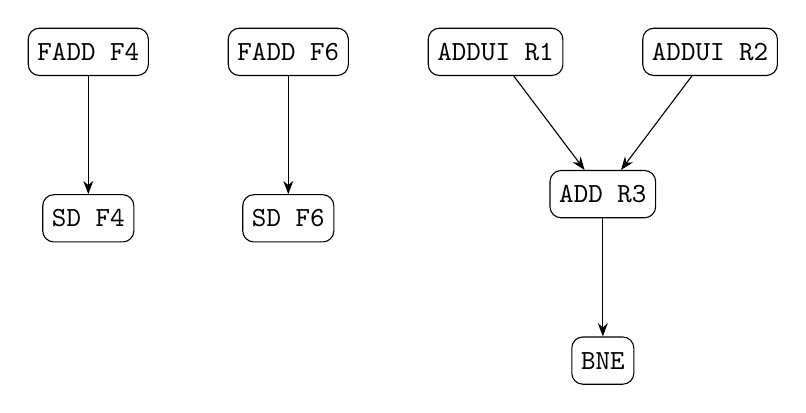
\begin{tikzpicture}[
            node distance=1.5cm and 1cm,
            box/.style={draw, rectangle, rounded corners, minimum size=6mm, align=center},
            >=Stealth
        ]
            % FADD nodes
            \node[box] (B1) {\texttt{FADD F4}};
            \node[box, right=of B1] (B2) {\texttt{FADD F6}};

            % SD nodes
            \node[box, below=of B1] (A1) {\texttt{SD F4}};
            \node[box, below=of B2] (A2) {\texttt{SD F6}};

            % ADDUI nodes
            \node[box, right=of B2] (D1) {\texttt{ADDUI R1}};
            \node[box, right=of D1] (D2) {\texttt{ADDUI R2}};

            % ADD and BNE
            \node[box, below=of $(D1)!0.5!(D2)$] (E1) {\texttt{ADD R3}};
            \node[box, below=of E1] (E2) {\texttt{BNE}};

            % Edges
            \draw[->] (B1) -- (A1);
            \draw[->] (B2) -- (A2);

            \draw[->] (D1) -- (E1);
            \draw[->] (D2) -- (E1);
            \draw[->] (E1) -- (E2);
        \end{tikzpicture}
    \end{center}

    \newpage

    \item \emph{What performance did you achieve in CPI?}

    \textcolor{Green3}{\textbf{\emph{Answer:}}} The Clock Per Instruction (CPI) can be calculated using the following formula:
    \begin{equation*}
        \text{CPI} = \dfrac{\text{\# Clock Cycles}}{\text{IC}} = \dfrac{\text{\# Clock Cycles}}{\text{\# Instructions}} = \dfrac{8}{10} = 0.8
    \end{equation*}


    \item \emph{What performance did you achieve in FP ops per cycles?}
    
    \textcolor{Green3}{\textbf{\emph{Answer:}}} FP ops per cycle measures \textbf{how well we are utilizing the FP functional units}. Here, there are 2 floating-point additions (\texttt{FADD F4}, \texttt{FADD F6}):
    \begin{equation*}
        \text{FP ops / cycle} = \dfrac{\text{\# Floating-Point ops}}{\text{\# Instructions}} = \dfrac{2}{8} = 0.25
    \end{equation*}


    \item \emph{How much is the code efficiency?}
    
    \textcolor{Green3}{\textbf{\emph{Answer:}}} When asked for \textbf{code efficiency} in this VLIW/ILP context, they usually mean:
    \begin{equation*}
        \text{Efficiency} = \frac{\text{Achieved IPC}}{\text{Maximum Theoretical IPC}}
    \end{equation*}
    So we measure \textbf{how much of the machine's peak parallelism we actually use}. The achieved Instruction Per Cycle (IPC) is:
    \begin{equation*}
        \text{Achieved IPC} = \dfrac{\text{\# Instructions}}{\text{\# Clock Cycles}} \dfrac{10}{8} = 1.25
    \end{equation*}
    Here, VLIW is 3-issue, so it can execute up to \textbf{3 ops per cycle} if there's no data or resource limit ($\text{Peak IPC} = 3$). So, code efficiency is:
    \begin{equation*}
        \text{Efficiency} = \frac{1.25}{3} = 0.4167 \approx 41.67\% \approx 42\%
    \end{equation*}
    \hl{We're achieving about 41.67\%} ($\approx 42 \%$) of the maximum possible execution parallelism.
\end{enumerate}

\newpage

\subsubsection*{Exercise 2.A - Dependency Analysis}

\emph{Consider the same software pipelined loop of \textbf{Exercise 1.A} containing multiple types of intra-loop dependences. Complete the following table by inserting all types of true-data-dependences, anti-
dependences and output dependences for each instruction:}

\highspace
\textcolor{Green3}{\textbf{\emph{Answer:}}}

\begin{table}[!htp]
    \centering
    \begin{tabular}{@{} l | l | p{20em} @{}}
        \toprule
        \texttt{I\#} & \textbf{Type of instruction}   & \textbf{Analysis of dependences:} \begin{enumerate}
            \item True data dependence with \texttt{I\#} for \texttt{\$Fx}
            \item Anti-dependence with \texttt{I\#} for \texttt{\$Fy}
            \item Output-dependence with \texttt{I\#} for \texttt{\$Fz}
        \end{enumerate} \\
        \midrule
        I1  & \texttt{SD F4, 0 (R1)} & None \\ [.3em]
        I2  & \texttt{SD F6, 0 (R2)} & None \\ [.3em]
        I3  & \texttt{FADD F4, F0, F0} & Anti-dependence with \texttt{I1} for \texttt{F4} \\ [.3em]
        I4  & \texttt{FADD F6, F2, F2} & Anti-dependence with \texttt{I2} for \texttt{F6} \\ [.3em]
        I5  & \texttt{LD F0, 16 (R1)} & Anti-dependence with \texttt{I3} for \texttt{F0} \\ [.3em]
        I6  & \texttt{LD F2, 16 (R2)} & Anti-dependence with \texttt{I4} for \texttt{F2} \\ [.3em]
        I7  & \texttt{ADDUI R1, R1, 8} & Anti-dependence with \texttt{I1} for \texttt{R1} \newline Anti-dependence with \texttt{I5} for \texttt{R1} \\ [.3em]
        I8  & \texttt{ADDUI R2, R2, 8} & Anti-dependence with \texttt{I2} for \texttt{R2} \newline Anti-dependence with \texttt{I6} for \texttt{R2} \\ [.3em]
        I9  & \texttt{ADD R3, R2, R1} & True data dependence with \texttt{I7} for \texttt{R1} \newline True data dependence with \texttt{I8} for \texttt{R2} \\ [.3em]
        I10 & \texttt{BNE R3, R4, SP\_LOOP} & True data dependence with \texttt{I9} for \texttt{R3} \\
        \bottomrule
    \end{tabular}
\end{table}

\newpage

\subsubsection*{Exercise 2.B - Tomasulo}

\emph{Consider the same assembly code to be executed on a CPU with dynamic scheduling based on \textbf{Tomasulo algorithm} with all cache HITS, a single Common Data Bus and:}
\begin{itemize}
    \item \emph{2 RESERVATION STATIONS (\textbf{RS1}, \textbf{RS2}) with 2 LOAD/STORE units (\textbf{LDU1}, \textbf{LDU2}) with latency \textbf{4}}
    \item \emph{2 RESERVATION STATIONS (\textbf{RS3}, \textbf{RS4}) with 1 FP unit (\textbf{FPU1}) with latency \textbf{4}}
    \item \emph{2 RESERVATION STATIONS (\textbf{RS5}, \textbf{RS6}) with 2 INT\_ALU/BR units (\textbf{ALU1}, \textbf{ALU2}) with latency \textbf{2}}
\end{itemize}
\emph{Please complete the following table:}

\highspace
\textcolor{Green3}{\textbf{\emph{Answer:}}} Before solving the Tomasulo, we need to remember how it is composed (see page \pageref{fig: tomasulo fpu}).

\begin{table}[!htp]
    \centering
    \begin{adjustbox}{width={\textwidth},totalheight={\textheight},keepaspectratio}
    \begin{tabular}{@{} l c c c c c c @{}}
        \toprule
        \textbf{Instruction} & \textbf{Issue} & \textbf{Start Exec} & \textbf{Write Res} & \textbf{Hazard} & \textbf{RSi} & \textbf{Unit} \\
        \midrule
        \texttt{I1: SD F4, 0 (R1)}      & \hl{1} & 2 & 6 & None  & \hl{\texttt{RS1}}   & \texttt{LDU1}  \\ [.5em]
        \texttt{I2: SD F6, 0 (R2)}      & 2 & 3 & 7 & None  & \texttt{RS2}   & \texttt{LDU2}  \\ [.5em]
        \texttt{I3: FADD F4, F0, F0}    &   &   &   &       &       &       \\ [.5em]
        \texttt{I4: FADD F6, F2, F2}    &   &   &   &       &       &       \\ [.5em]
        \texttt{I5: LD F0, 16 (R1)}     &   &   &   &       &       &       \\ [.5em]
        \texttt{I6: LD F2, 16 (R2)}     &   &   &   &       &       &       \\ [.5em]
        \texttt{I7: ADDUI R1, R1, 8}    &   &   &   &       &       &       \\ [.5em]
        \texttt{I8: ADDUI R2, R2, 8}    &   &   &   &       &       &       \\ [.5em]
        \texttt{I9: ADD R3, R2, R1}     &   &   &   &       &       &       \\ [.5em]
        \texttt{I10: BNE R3, R4, LOOP}   &   &   &   &       &       &       \\
        \bottomrule
    \end{tabular}
    \end{adjustbox}
\end{table}

% \begin{minipage}{0.45\textwidth}
%     \centering
%     \begin{tabular}{@{} l | l l l l @{}}
%         \toprule
%         & \texttt{Vj} & \texttt{Qj} & \texttt{Vk} & \texttt{Qk} \\
%         \midrule
%         RS1 & & & \\ [.3em]
%         RS2 & & & \\ [.3em]
%         \cmidrule{1-5}
%         LDU1 & & & \\ [.3em]
%         LDU2 & & & \\
%         \bottomrule
%     \end{tabular}
% \end{minipage}
% \hfill
% \begin{minipage}{0.45\textwidth}
%     \centering
%     \begin{tabular}{@{} l | l l l l @{}}
%         \toprule
%         & \texttt{Vj} & \texttt{Qj} & \texttt{Vk} & \texttt{Qk} \\
%         \midrule
%         RS3 & & & \\ [.3em]
%         RS4 & & & \\ [.3em]
%         \cmidrule{1-5}
%         FPU1 & & & \\
%         \bottomrule
%     \end{tabular}
% \end{minipage}
% 
% \begin{center}
%     \begin{tabular}{@{} l | l l l l @{}}
%         \toprule
%         & \texttt{Vj} & \texttt{Qj} & \texttt{Vk} & \texttt{Qk} \\
%         \midrule
%         RS5 & & & \\ [.3em]
%         RS6 & & & \\ [.3em]
%         \cmidrule{1-5}
%         ALU1 & & & \\ [.3em]
%         ALU2 & & & \\
%         \bottomrule
%     \end{tabular}
% \end{center}

\begin{enumerate}
    \item \textbf{Cycle \theenumi}:
    
    \begin{minipage}{0.45\textwidth}
        \centering
        \begin{tabular}{@{} l | l l l l @{}}
            \toprule
                & \texttt{Vj} & \texttt{Qj} & \texttt{Vk} & \texttt{Qk} \\
            \midrule
            \texttt{RS1} & \hl{\texttt{F4}} & & \hl{\texttt{-}} & \\ [.3em]
            \texttt{RS2} & & & & \\ [.3em]
            \cmidrule{1-5}
            \texttt{LDU1} & & & & \\ [.3em]
            \texttt{LDU2} & & & & \\
            \bottomrule
        \end{tabular}
    \end{minipage}
    \hfill
    \begin{minipage}{0.45\textwidth}
        \centering
        \begin{tabular}{@{} l | l l l l @{}}
            \toprule
            & \texttt{Vj} & \texttt{Qj} & \texttt{Vk} & \texttt{Qk} \\
            \midrule
            \texttt{RS3} & & & & \\ [.3em]
            \texttt{RS4} & & & & \\ [.3em]
            \cmidrule{1-5}
            \texttt{FPU1} & & & & \\
            \bottomrule
        \end{tabular}
    \end{minipage}

    \begin{center}
        \begin{tabular}{@{} l | l l l l @{}}
            \toprule
            & \texttt{Vj} & \texttt{Qj} & \texttt{Vk} & \texttt{Qk} \\
            \midrule
            \texttt{RS5} & & & & \\ [.3em]
            \texttt{RS6} & & & & \\ [.3em]
            \cmidrule{1-5}
            \texttt{ALU1} & & & & \\ [.3em]
            \texttt{ALU2} & & & & \\
            \bottomrule
        \end{tabular}
    \end{center}
    \newpage
    


    %%%%%%%%%%%%%%%%%%%%%%%%%%%%%%%%%%%%%%%%%%%%%%%%%%%%%%%%%%%%%%%%%%%%%%%%%%%%%%%%%%%%%%%%%%%%%%%%%%%%%%%%
    \item \textbf{Cycle \theenumi}:
    
    \begin{table}[!htp]
        \centering
        \begin{adjustbox}{width={\textwidth},totalheight={\textheight},keepaspectratio}
        \begin{tabular}{@{} l c c c c c c @{}}
            \toprule
            \textbf{Instruction} & \textbf{Issue} & \textbf{Start Exec} & \textbf{Write Res} & \textbf{Hazard} & \textbf{RSi} & \textbf{Unit} \\
            \midrule
            \texttt{I1: SD F4, 0 (R1)}      & 1 & \hl{2} & 6 & None  & \texttt{RS1}   & \hl{\texttt{LDU1}}  \\ [.5em]
            \texttt{I2: SD F6, 0 (R2)}      & \hl{2} & 3 & 7 & None  & \hl{\texttt{RS2}}   & \texttt{LDU2}  \\ [.5em]
            \texttt{I3: FADD F4, F0, F0}    &   &   &   &       &       &       \\ [.5em]
            \texttt{I4: FADD F6, F2, F2}    &   &   &   &       &       &       \\ [.5em]
            \texttt{I5: LD F0, 16 (R1)}     &   &   &   &       &       &       \\ [.5em]
            \texttt{I6: LD F2, 16 (R2)}     &   &   &   &       &       &       \\ [.5em]
            \texttt{I7: ADDUI R1, R1, 8}    &   &   &   &       &       &       \\ [.5em]
            \texttt{I8: ADDUI R2, R2, 8}    &   &   &   &       &       &       \\ [.5em]
            \texttt{I9: ADD R3, R2, R1}     &   &   &   &       &       &       \\ [.5em]
            \texttt{I10: BNE R3, R4, LOOP}   &   &   &   &       &       &       \\
            \bottomrule
        \end{tabular}
        \end{adjustbox}
    \end{table}
    
    \begin{minipage}{0.45\textwidth}
        \centering
        \begin{tabular}{@{} l | l l l l @{}}
            \toprule
                & \texttt{Vj} & \texttt{Qj} & \texttt{Vk} & \texttt{Qk} \\
            \midrule
            \texttt{RS1} & \texttt{F4} & & \texttt{-} & \\ [.3em]
            \texttt{RS2} & \hl{\texttt{F6}} & & \hl{\texttt{-}} & \\
            \cmidrule{1-5}
            \texttt{LDU1} & \hl{\texttt{F4}} & & \hl{\texttt{-}} & \\ [.3em]
            \texttt{LDU2} & & & & \\
            \bottomrule
        \end{tabular}
    \end{minipage}
    \hfill
    \begin{minipage}{0.45\textwidth}
        \centering
        \begin{tabular}{@{} l | l l l l @{}}
            \toprule
            & \texttt{Vj} & \texttt{Qj} & \texttt{Vk} & \texttt{Qk} \\
            \midrule
            \texttt{RS3} & & & & \\ [.3em]
            \texttt{RS4} & & & & \\
            \cmidrule{1-5}
            \texttt{FPU1} & & & & \\
            \bottomrule
        \end{tabular}
    \end{minipage}

    \begin{minipage}{0.45\textwidth}
        \centering
        \begin{tabular}{@{} l | l l l l @{}}
            \toprule
            & \texttt{Vj} & \texttt{Qj} & \texttt{Vk} & \texttt{Qk} \\
            \midrule
            \texttt{RS5} & & & & \\ [.3em]
            \texttt{RS6} & & & & \\
            \cmidrule{1-5}
            \texttt{ALU1} & & & & \\ [.3em]
            \texttt{ALU2} & & & & \\
            \bottomrule
        \end{tabular}
    \end{minipage}
    \hfill
    \begin{minipage}{0.45\textwidth}
        \centering
        \begin{tabular}{@{} l c @{}}
            \toprule
            Unit            & Remaining cycles \\
            \midrule
            \texttt{LDU1}   & 4 \\ [.3em]
            \texttt{LDU2}   & \\ [.3em]
            \texttt{FPU1}   & \\ [.3em]
            \texttt{ALU1}   & \\ [.3em]
            \texttt{ALU2}   & \\
            \bottomrule
        \end{tabular}
    \end{minipage}
    \newpage




    %%%%%%%%%%%%%%%%%%%%%%%%%%%%%%%%%%%%%%%%%%%%%%%%%%%%%%%%%%%%%%%%%%%%%%%%%%%%%%%%%%%%%%%%%%%%%%%%%%%%%%%%
    \item \textbf{Cycle \theenumi}: Here, we have a anti-dependence hazard (WAR) because the third instruction writes the sum to register \texttt{F4} and the first instruction reads \texttt{F4}. In Tomasulo, though, we don't care about this because the issue stage stalls if and only if there are no reservation stations, the Load/Store queue is full (for memory ops), or for speculative instructions (for prediction, which is not our case). Therefore, we issue and start execution. At the end of execution, we will determine whether to write the result or wait.
    
    \begin{table}[!htp]
        \centering
        \begin{adjustbox}{width={\textwidth},totalheight={\textheight},keepaspectratio}
        \begin{tabular}{@{} l c c c c c c @{}}
            \toprule
            \textbf{Instruction} & \textbf{Issue} & \textbf{Start Exec} & \textbf{Write Res} & \textbf{Hazard} & \textbf{RSi} & \textbf{Unit} \\
            \midrule
            \texttt{I1: SD F4, 0 (R1)}      & 1 & 2 & 6 & None  & \texttt{RS1}   & \texttt{LDU1}  \\ [.5em]
            \texttt{I2: SD F6, 0 (R2)}      & 2 & \hl{3} & 7 & None  & \texttt{RS2}   & \hl{\texttt{LDU2}}  \\ [.5em]
            \texttt{I3: FADD F4, F0, F0}    & \hl{3} &   &   & \hl{\texttt{WAR I1, F4}} & \hl{\texttt{RS3}} &       \\ [.5em]
            \texttt{I4: FADD F6, F2, F2}    &   &   &   &       &       &       \\ [.5em]
            \texttt{I5: LD F0, 16 (R1)}     &   &   &   &       &       &       \\ [.5em]
            \texttt{I6: LD F2, 16 (R2)}     &   &   &   &       &       &       \\ [.5em]
            \texttt{I7: ADDUI R1, R1, 8}    &   &   &   &       &       &       \\ [.5em]
            \texttt{I8: ADDUI R2, R2, 8}    &   &   &   &       &       &       \\ [.5em]
            \texttt{I9: ADD R3, R2, R1}     &   &   &   &       &       &       \\ [.5em]
            \texttt{I10: BNE R3, R4, LOOP}   &   &   &   &       &       &       \\
            \bottomrule
        \end{tabular}
        \end{adjustbox}
    \end{table}
    
    \begin{minipage}{0.45\textwidth}
        \centering
        \begin{tabular}{@{} l | l l l l @{}}
            \toprule
                & \texttt{Vj} & \texttt{Qj} & \texttt{Vk} & \texttt{Qk} \\
            \midrule
            \texttt{RS1} & \texttt{F4} & & \texttt{-} & \\ [.3em]
            \texttt{RS2} & \texttt{F6} & & \texttt{-} & \\
            \cmidrule{1-5}
            \texttt{LDU1} & \texttt{F4} & & \texttt{-} & \\ [.3em]
            \texttt{LDU2} & \hl{\texttt{F6}} & & \hl{\texttt{-}} & \\
            \bottomrule
        \end{tabular}
    \end{minipage}
    \hfill
    \begin{minipage}{0.45\textwidth}
        \centering
        \begin{tabular}{@{} l | l l l l @{}}
            \toprule
            & \texttt{Vj} & \texttt{Qj} & \texttt{Vk} & \texttt{Qk} \\
            \midrule
            \texttt{RS3} & \hl{\texttt{F0}} & & \hl{\texttt{F0}} & \\ [.3em]
            \texttt{RS4} & & & & \\
            \cmidrule{1-5}
            \texttt{FPU1} & & & & \\
            \bottomrule
        \end{tabular}
    \end{minipage}

    \begin{minipage}{0.45\textwidth}
        \centering
        \begin{tabular}{@{} l | l l l l @{}}
            \toprule
            & \texttt{Vj} & \texttt{Qj} & \texttt{Vk} & \texttt{Qk} \\
            \midrule
            \texttt{RS5} & & & & \\ [.3em]
            \texttt{RS6} & & & & \\
            \cmidrule{1-5}
            \texttt{ALU1} & & & & \\ [.3em]
            \texttt{ALU2} & & & & \\
            \bottomrule
        \end{tabular}
    \end{minipage}
    \hfill
    \begin{minipage}{0.45\textwidth}
        \centering
        \begin{tabular}{@{} l c @{}}
            \toprule
            Unit            & Remaining cycles \\
            \midrule
            \texttt{LDU1}   & 3 \\ [.3em]
            \texttt{LDU2}   & 4 \\ [.3em]
            \texttt{FPU1}   & \\ [.3em]
            \texttt{ALU1}   & \\ [.3em]
            \texttt{ALU2}   & \\
            \bottomrule
        \end{tabular}
    \end{minipage}
    \newpage




    %%%%%%%%%%%%%%%%%%%%%%%%%%%%%%%%%%%%%%%%%%%%%%%%%%%%%%%%%%%%%%%%%%%%%%%%%%%%%%%%%%%%%%%%%%%%%%%%%%%%%%%%
    \item \textbf{Cycle \theenumi}: It's the same situation as before with the hazard (WAR), but now it's \texttt{I4} with \texttt{I2}.
    
    \begin{table}[!htp]
        \centering
        \begin{adjustbox}{width={\textwidth},totalheight={\textheight},keepaspectratio}
        \begin{tabular}{@{} l c c c c c c @{}}
            \toprule
            \textbf{Instruction} & \textbf{Issue} & \textbf{Start Exec} & \textbf{Write Res} & \textbf{Hazard} & \textbf{RSi} & \textbf{Unit} \\
            \midrule
            \texttt{I1: SD F4, 0 (R1)}      & 1 & 2 & 6 & None  & \texttt{RS1}   & \texttt{LDU1}  \\ [.5em]
            \texttt{I2: SD F6, 0 (R2)}      & 2 & 3 & 7 & None  & \texttt{RS2}   & \texttt{LDU2}  \\ [.5em]
            \texttt{I3: FADD F4, F0, F0}    & 3 & \hl{4} &   & \texttt{WAR I1, F4}  & \texttt{RS3} & \hl{\texttt{FPU1}} \\ [.5em]
            \texttt{I4: FADD F6, F2, F2}    & \hl{4} &   &   & \hl{\texttt{WAR I2, F6}} & \hl{\texttt{RS4}} &       \\ [.5em]
            \texttt{I5: LD F0, 16 (R1)}     &   &   &   &       &       &       \\ [.5em]
            \texttt{I6: LD F2, 16 (R2)}     &   &   &   &       &       &       \\ [.5em]
            \texttt{I7: ADDUI R1, R1, 8}    &   &   &   &       &       &       \\ [.5em]
            \texttt{I8: ADDUI R2, R2, 8}    &   &   &   &       &       &       \\ [.5em]
            \texttt{I9: ADD R3, R2, R1}     &   &   &   &       &       &       \\ [.5em]
            \texttt{I10: BNE R3, R4, LOOP}   &   &   &   &       &       &       \\
            \bottomrule
        \end{tabular}
        \end{adjustbox}
    \end{table}
    
    \begin{minipage}{0.45\textwidth}
        \centering
        \begin{tabular}{@{} l | l l l l @{}}
            \toprule
                & \texttt{Vj} & \texttt{Qj} & \texttt{Vk} & \texttt{Qk} \\
            \midrule
            \texttt{RS1} & \texttt{F4} & & \texttt{-} & \\ [.3em]
            \texttt{RS2} & \texttt{F6} & & \texttt{-} & \\
            \cmidrule{1-5}
            \texttt{LDU1} & \texttt{F4} & & \texttt{-} & \\ [.3em]
            \texttt{LDU2} & \texttt{F6} & & \texttt{-} & \\
            \bottomrule
        \end{tabular}
    \end{minipage}
    \hfill
    \begin{minipage}{0.45\textwidth}
        \centering
        \begin{tabular}{@{} l | l l l l @{}}
            \toprule
            & \texttt{Vj} & \texttt{Qj} & \texttt{Vk} & \texttt{Qk} \\
            \midrule
            \texttt{RS3} & \texttt{F0} & & \texttt{F0} & \\ [.3em]
            \texttt{RS4} & \hl{\texttt{F2}} & & \hl{\texttt{F2}} & \\
            \cmidrule{1-5}
            \texttt{FPU1} & \hl{\texttt{F0}} & & \hl{\texttt{F0}} & \\
            \bottomrule
        \end{tabular}
    \end{minipage}

    \begin{minipage}{0.45\textwidth}
        \centering
        \begin{tabular}{@{} l | l l l l @{}}
            \toprule
            & \texttt{Vj} & \texttt{Qj} & \texttt{Vk} & \texttt{Qk} \\
            \midrule
            \texttt{RS5} & & & & \\ [.3em]
            \texttt{RS6} & & & & \\
            \cmidrule{1-5}
            \texttt{ALU1} & & & & \\ [.3em]
            \texttt{ALU2} & & & & \\
            \bottomrule
        \end{tabular}
    \end{minipage}
    \hfill
    \begin{minipage}{0.45\textwidth}
        \centering
        \begin{tabular}{@{} l c @{}}
            \toprule
            Unit            & Remaining cycles \\
            \midrule
            \texttt{LDU1}   & 2 \\ [.3em]
            \texttt{LDU2}   & 3 \\ [.3em]
            \texttt{FPU1}   & 4 \\ [.3em]
            \texttt{ALU1}   & \\ [.3em]
            \texttt{ALU2}   & \\
            \bottomrule
        \end{tabular}
    \end{minipage}
    \newpage






    %%%%%%%%%%%%%%%%%%%%%%%%%%%%%%%%%%%%%%%%%%%%%%%%%%%%%%%%%%%%%%%%%%%%%%%%%%%%%%%%%%%%%%%%%%%%%%%%%%%%%%%%
    \item \textbf{Cycle \theenumi}: Instruction 4 cannot begin because there are no available functional units. Therefore, it remains idle at reservation station 4. Instructions 5 and 6 cannot start either because there are no load/store reservation units available. \texttt{ADDUI} operations cannot start because instructions 5 and 6 need to read the \texttt{R1} and \texttt{R2} registers (WAR hazard).
    
    \begin{table}[!htp]
        \centering
        \begin{adjustbox}{width={\textwidth},totalheight={\textheight},keepaspectratio}
        \begin{tabular}{@{} l c c c c c c @{}}
            \toprule
            \textbf{Instruction} & \textbf{Issue} & \textbf{Start Exec} & \textbf{Write Res} & \textbf{Hazard} & \textbf{RSi} & \textbf{Unit} \\
            \midrule
            \texttt{I1: SD F4, 0 (R1)}      & 1 & 2 & 6 & None  & \texttt{RS1}   & \texttt{LDU1}  \\ [.5em]
            \texttt{I2: SD F6, 0 (R2)}      & 2 & 3 & 7 & None  & \texttt{RS2}   & \texttt{LDU2}  \\ [.5em]
            \texttt{I3: FADD F4, F0, F0}    & 3 & 4 &   & \texttt{WAR I1, F4}  & \texttt{RS3} & \texttt{FPU1} \\ [.5em]
            \texttt{I4: FADD F6, F2, F2}    & 4 &   &   & \texttt{WAR I2, F6} & \texttt{RS4} &       \\ [.5em]
            \texttt{I5: LD F0, 16 (R1)}     &   &   &   & \hl{\texttt{WAR I3, F0}} &       &       \\ [.5em]
            \texttt{I6: LD F2, 16 (R2)}     &   &   &   & \hl{\texttt{WAR I4, F2}} &       &       \\ [.5em]
            \texttt{I7: ADDUI R1, R1, 8}    &   &   &   & \hl{\texttt{WAR I5, R1}} &       &       \\ [.5em]
            \texttt{I8: ADDUI R2, R2, 8}    &   &   &   & \hl{\texttt{WAR I6, R2}} &       &       \\ [.5em]
            \texttt{I9: ADD R3, R2, R1}     &   &   &   & \hl{\texttt{RAW R1, R2}} &       &       \\ [.5em]
            \texttt{I10: BNE R3, R4, LOOP}   &   &   &   & \hl{\texttt{RAW I9, R3}} &       &       \\
            \bottomrule
        \end{tabular}
        \end{adjustbox}
    \end{table}
    
    \begin{minipage}{0.45\textwidth}
        \centering
        \begin{tabular}{@{} l | l l l l @{}}
            \toprule
                & \texttt{Vj} & \texttt{Qj} & \texttt{Vk} & \texttt{Qk} \\
            \midrule
            \texttt{RS1} & \texttt{F4} & & \texttt{-} & \\ [.3em]
            \texttt{RS2} & \texttt{F6} & & \texttt{-} & \\
            \cmidrule{1-5}
            \texttt{LDU1} & \texttt{F4} & & \texttt{-} & \\ [.3em]
            \texttt{LDU2} & \texttt{F6} & & \texttt{-} & \\
            \bottomrule
        \end{tabular}
    \end{minipage}
    \hfill
    \begin{minipage}{0.45\textwidth}
        \centering
        \begin{tabular}{@{} l | l l l l @{}}
            \toprule
            & \texttt{Vj} & \texttt{Qj} & \texttt{Vk} & \texttt{Qk} \\
            \midrule
            \texttt{RS3} & \texttt{F0} & & \texttt{F0} & \\ [.3em]
            \texttt{RS4} & \texttt{F2} & & \texttt{F2} & \\
            \cmidrule{1-5}
            \texttt{FPU1} & \texttt{F0} & & \texttt{F0} & \\
            \bottomrule
        \end{tabular}
    \end{minipage}

    \begin{minipage}{0.45\textwidth}
        \centering
        \begin{tabular}{@{} l | l l l l @{}}
            \toprule
            & \texttt{Vj} & \texttt{Qj} & \texttt{Vk} & \texttt{Qk} \\
            \midrule
            \texttt{RS5} & & & & \\ [.3em]
            \texttt{RS6} & & & & \\
            \cmidrule{1-5}
            \texttt{ALU1} & & & & \\ [.3em]
            \texttt{ALU2} & & & & \\
            \bottomrule
        \end{tabular}
    \end{minipage}
    \hfill
    \begin{minipage}{0.45\textwidth}
        \centering
        \begin{tabular}{@{} l c @{}}
            \toprule
            Unit            & Remaining cycles \\
            \midrule
            \texttt{LDU1}   & 1 \\ [.3em]
            \texttt{LDU2}   & 2 \\ [.3em]
            \texttt{FPU1}   & 3 \\ [.3em]
            \texttt{ALU1}   & \\ [.3em]
            \texttt{ALU2}   & \\
            \bottomrule
        \end{tabular}
    \end{minipage}
    \newpage





    %%%%%%%%%%%%%%%%%%%%%%%%%%%%%%%%%%%%%%%%%%%%%%%%%%%%%%%%%%%%%%%%%%%%%%%%%%%%%%%%%%%%%%%%%%%%%%%%%%%%%%%%
    \item \textbf{Cycle \theenumi}:
    
    \begin{table}[!htp]
        \centering
        \begin{adjustbox}{width={\textwidth},totalheight={\textheight},keepaspectratio}
        \begin{tabular}{@{} l c c c c c c @{}}
            \toprule
            \textbf{Instruction} & \textbf{Issue} & \textbf{Start Exec} & \textbf{Write Res} & \textbf{Hazard} & \textbf{RSi} & \textbf{Unit} \\
            \midrule
            \texttt{I1: SD F4, 0 (R1)}      & 1 & 2 & \hl{6} & None  & \texttt{RS1}   & \texttt{LDU1}  \\ [.5em]
            \texttt{I2: SD F6, 0 (R2)}      & 2 & 3 & 7 & None  & \texttt{RS2}   & \texttt{LDU2}  \\ [.5em]
            \texttt{I3: FADD F4, F0, F0}    & 3 & 4 &   & \texttt{WAR I1, F4}  & \texttt{RS3} & \texttt{FPU1} \\ [.5em]
            \texttt{I4: FADD F6, F2, F2}    & 4 &   &   & \texttt{WAR I2, F6} & \texttt{RS4} &       \\ [.5em]
            \texttt{I5: LD F0, 16 (R1)}     &   &   &   & \texttt{WAR I3, F0} &       &       \\ [.5em]
            \texttt{I6: LD F2, 16 (R2)}     &   &   &   & \texttt{WAR I4, F2} &       &       \\ [.5em]
            \texttt{I7: ADDUI R1, R1, 8}    &   &   &   & \texttt{WAR I5, R1} &       &       \\ [.5em]
            \texttt{I8: ADDUI R2, R2, 8}    &   &   &   & \texttt{WAR I6, R2} &       &       \\ [.5em]
            \texttt{I9: ADD R3, R2, R1}     &   &   &   & \texttt{RAW R1, R2} &       &       \\ [.5em]
            \texttt{I10: BNE R3, R4, LOOP}   &   &   &   & \texttt{RAW I9, R3} &       &       \\
            \bottomrule
        \end{tabular}
        \end{adjustbox}
    \end{table}
    
    \begin{minipage}{0.45\textwidth}
        \centering
        \begin{tabular}{@{} l | l l l l @{}}
            \toprule
                & \texttt{Vj} & \texttt{Qj} & \texttt{Vk} & \texttt{Qk} \\
            \midrule
            \texttt{RS1} & \texttt{F4} & & \texttt{-} & \\ [.3em]
            \texttt{RS2} & \texttt{F6} & & \texttt{-} & \\
            \cmidrule{1-5}
            \texttt{LDU1} & \texttt{F4} & & \texttt{-} & \\ [.3em]
            \texttt{LDU2} & \texttt{F6} & & \texttt{-} & \\
            \bottomrule
        \end{tabular}
    \end{minipage}
    \hfill
    \begin{minipage}{0.45\textwidth}
        \centering
        \begin{tabular}{@{} l | l l l l @{}}
            \toprule
            & \texttt{Vj} & \texttt{Qj} & \texttt{Vk} & \texttt{Qk} \\
            \midrule
            \texttt{RS3} & \texttt{F0} & & \texttt{F0} & \\ [.3em]
            \texttt{RS4} & \texttt{F2} & & \texttt{F2} & \\
            \cmidrule{1-5}
            \texttt{FPU1} & \texttt{F0} & & \texttt{F0} & \\
            \bottomrule
        \end{tabular}
    \end{minipage}

    \begin{minipage}{0.45\textwidth}
        \centering
        \begin{tabular}{@{} l | l l l l @{}}
            \toprule
            & \texttt{Vj} & \texttt{Qj} & \texttt{Vk} & \texttt{Qk} \\
            \midrule
            \texttt{RS5} & & & & \\ [.3em]
            \texttt{RS6} & & & & \\
            \cmidrule{1-5}
            \texttt{ALU1} & & & & \\ [.3em]
            \texttt{ALU2} & & & & \\
            \bottomrule
        \end{tabular}
    \end{minipage}
    \hfill
    \begin{minipage}{0.45\textwidth}
        \centering
        \begin{tabular}{@{} l c @{}}
            \toprule
            Unit            & Remaining cycles \\
            \midrule
            \texttt{LDU1}   & 0 \\ [.3em]
            \texttt{LDU2}   & 1 \\ [.3em]
            \texttt{FPU1}   & 2 \\ [.3em]
            \texttt{ALU1}   & \\ [.3em]
            \texttt{ALU2}   & \\
            \bottomrule
        \end{tabular}
    \end{minipage}
    \newpage





    %%%%%%%%%%%%%%%%%%%%%%%%%%%%%%%%%%%%%%%%%%%%%%%%%%%%%%%%%%%%%%%%%%%%%%%%%%%%%%%%%%%%%%%%%%%%%%%%%%%%%%%%
    \item \textbf{Cycle \theenumi}:
    
    \begin{table}[!htp]
        \centering
        \begin{adjustbox}{width={\textwidth},totalheight={\textheight},keepaspectratio}
        \begin{tabular}{@{} l c c c c c c @{}}
            \toprule
            \textbf{Instruction} & \textbf{Issue} & \textbf{Start Exec} & \textbf{Write Res} & \textbf{Hazard} & \textbf{RSi} & \textbf{Unit} \\
            \midrule
            \texttt{I1: SD F4, 0 (R1)}      & 1 & 2 & 6 & None  & \texttt{RS1}   & \texttt{LDU1}  \\ [.5em]
            \texttt{I2: SD F6, 0 (R2)}      & 2 & 3 & \hl{7} & None  & \texttt{RS2}   & \texttt{LDU2}  \\ [.5em]
            \texttt{I3: FADD F4, F0, F0}    & 3 & 4 &   & \texttt{WAR I1, F4}  & \texttt{RS3} & \texttt{FPU1} \\ [.5em]
            \texttt{I4: FADD F6, F2, F2}    & 4 &   &   & \texttt{WAR I2, F6} & \texttt{RS4} &       \\ [.5em]
            \texttt{I5: LD F0, 16 (R1)}     & \hl{7} &   &   & \texttt{WAR I3, F0} & \hl{\texttt{RS1}} &       \\ [.5em]
            \texttt{I6: LD F2, 16 (R2)}     &   &   &   & \texttt{WAR I4, F2} &       &       \\ [.5em]
            \texttt{I7: ADDUI R1, R1, 8}    &   &   &   & \texttt{WAR I5, R1} &       &       \\ [.5em]
            \texttt{I8: ADDUI R2, R2, 8}    &   &   &   & \texttt{WAR I6, R2} &       &       \\ [.5em]
            \texttt{I9: ADD R3, R2, R1}     &   &   &   & \texttt{RAW R1, R2} &       &       \\ [.5em]
            \texttt{I10: BNE R3, R4, LOOP}   &   &   &   & \texttt{RAW I9, R3} &       &       \\
            \bottomrule
        \end{tabular}
        \end{adjustbox}
    \end{table}
    
    \begin{minipage}{0.45\textwidth}
        \centering
        \begin{tabular}{@{} l | l l l l @{}}
            \toprule
                & \texttt{Vj} & \texttt{Qj} & \texttt{Vk} & \texttt{Qk} \\
            \midrule
            \texttt{RS1} & \hl{\texttt{16}} & & \hl{\texttt{R1}} & \\ [.3em]
            \texttt{RS2} & \texttt{F6} & & \texttt{-} & \\
            \cmidrule{1-5}
            \texttt{LDU1} & & & & \\ [.3em]
            \texttt{LDU2} & \texttt{F6} & & \texttt{-} & \\
            \bottomrule
        \end{tabular}
    \end{minipage}
    \hfill
    \begin{minipage}{0.45\textwidth}
        \centering
        \begin{tabular}{@{} l | l l l l @{}}
            \toprule
            & \texttt{Vj} & \texttt{Qj} & \texttt{Vk} & \texttt{Qk} \\
            \midrule
            \texttt{RS3} & \texttt{F0} & & \texttt{F0} & \\ [.3em]
            \texttt{RS4} & \texttt{F2} & & \texttt{F2} & \\
            \cmidrule{1-5}
            \texttt{FPU1} & \texttt{F0} & & \texttt{F0} & \\
            \bottomrule
        \end{tabular}
    \end{minipage}

    \begin{minipage}{0.45\textwidth}
        \centering
        \begin{tabular}{@{} l | l l l l @{}}
            \toprule
            & \texttt{Vj} & \texttt{Qj} & \texttt{Vk} & \texttt{Qk} \\
            \midrule
            \texttt{RS5} & & & & \\ [.3em]
            \texttt{RS6} & & & & \\
            \cmidrule{1-5}
            \texttt{ALU1} & & & & \\ [.3em]
            \texttt{ALU2} & & & & \\
            \bottomrule
        \end{tabular}
    \end{minipage}
    \hfill
    \begin{minipage}{0.45\textwidth}
        \centering
        \begin{tabular}{@{} l c @{}}
            \toprule
            Unit            & Remaining cycles \\
            \midrule
            \texttt{LDU1}   & \\ [.3em]
            \texttt{LDU2}   & 0 \\ [.3em]
            \texttt{FPU1}   & 1 \\ [.3em]
            \texttt{ALU1}   & \\ [.3em]
            \texttt{ALU2}   & \\
            \bottomrule
        \end{tabular}
    \end{minipage}
    \newpage





    %%%%%%%%%%%%%%%%%%%%%%%%%%%%%%%%%%%%%%%%%%%%%%%%%%%%%%%%%%%%%%%%%%%%%%%%%%%%%%%%%%%%%%%%%%%%%%%%%%%%%%%%
    \item \textbf{Cycle \theenumi}:
    
    \begin{table}[!htp]
        \centering
        \begin{adjustbox}{width={\textwidth},totalheight={\textheight},keepaspectratio}
        \begin{tabular}{@{} l c c c c c c @{}}
            \toprule
            \textbf{Instruction} & \textbf{Issue} & \textbf{Start Exec} & \textbf{Write Res} & \textbf{Hazard} & \textbf{RSi} & \textbf{Unit} \\
            \midrule
            \texttt{I1: SD F4, 0 (R1)}      & 1 & 2 & 6 & None  & \texttt{RS1}   & \texttt{LDU1}  \\ [.5em]
            \texttt{I2: SD F6, 0 (R2)}      & 2 & 3 & 7 & None  & \texttt{RS2}   & \texttt{LDU2}  \\ [.5em]
            \texttt{I3: FADD F4, F0, F0}    & 3 & 4 & \hl{8} & \texttt{WAR I1, F4}  & \texttt{RS3} & \texttt{FPU1} \\ [.5em]
            \texttt{I4: FADD F6, F2, F2}    & 4 &   &   & \texttt{WAR I2, F6} & \texttt{RS4} &       \\ [.5em]
            \texttt{I5: LD F0, 16 (R1)}     & 7 & \hl{8} &   & \texttt{WAR I3, F0} & \texttt{RS1} & \hl{\texttt{LDU1}} \\ [.5em]
            \texttt{I6: LD F2, 16 (R2)}     & \hl{8} &   &   & \texttt{WAR I4, F2} & \hl{\texttt{RS2}} &       \\ [.5em]
            \texttt{I7: ADDUI R1, R1, 8}    &   &   &   & \texttt{WAR I5, R1} &       &       \\ [.5em]
            \texttt{I8: ADDUI R2, R2, 8}    &   &   &   & \texttt{WAR I6, R2} &       &       \\ [.5em]
            \texttt{I9: ADD R3, R2, R1}     &   &   &   & \texttt{RAW R1, R2} &       &       \\ [.5em]
            \texttt{I10: BNE R3, R4, LOOP}   &   &   &   & \texttt{RAW I9, R3} &       &       \\
            \bottomrule
        \end{tabular}
        \end{adjustbox}
    \end{table}
    
    \begin{minipage}{0.45\textwidth}
        \centering
        \begin{tabular}{@{} l | l l l l @{}}
            \toprule
                & \texttt{Vj} & \texttt{Qj} & \texttt{Vk} & \texttt{Qk} \\
            \midrule
            \texttt{RS1} & \texttt{16} & & \texttt{R1} & \\ [.3em]
            \texttt{RS2} & \hl{\texttt{16}} & & \hl{\texttt{R2}} & \\
            \cmidrule{1-5}
            \texttt{LDU1} & \hl{\texttt{16}} & & \hl{\texttt{R1}} & \\ [.3em]
            \texttt{LDU2} & & & & \\
            \bottomrule
        \end{tabular}
    \end{minipage}
    \hfill
    \begin{minipage}{0.45\textwidth}
        \centering
        \begin{tabular}{@{} l | l l l l @{}}
            \toprule
            & \texttt{Vj} & \texttt{Qj} & \texttt{Vk} & \texttt{Qk} \\
            \midrule
            \texttt{RS3} & \texttt{F0} & & \texttt{F0} & \\ [.3em]
            \texttt{RS4} & \texttt{F2} & & \texttt{F2} & \\
            \cmidrule{1-5}
            \texttt{FPU1} & \texttt{F0} & & \texttt{F0} & \\
            \bottomrule
        \end{tabular}
    \end{minipage}

    \begin{minipage}{0.45\textwidth}
        \centering
        \begin{tabular}{@{} l | l l l l @{}}
            \toprule
            & \texttt{Vj} & \texttt{Qj} & \texttt{Vk} & \texttt{Qk} \\
            \midrule
            \texttt{RS5} & & & & \\ [.3em]
            \texttt{RS6} & & & & \\
            \cmidrule{1-5}
            \texttt{ALU1} & & & & \\ [.3em]
            \texttt{ALU2} & & & & \\
            \bottomrule
        \end{tabular}
    \end{minipage}
    \hfill
    \begin{minipage}{0.45\textwidth}
        \centering
        \begin{tabular}{@{} l c @{}}
            \toprule
            Unit            & Remaining cycles \\
            \midrule
            \texttt{LDU1}   & 4 \\ [.3em]
            \texttt{LDU2}   & \\ [.3em]
            \texttt{FPU1}   & 0 \\ [.3em]
            \texttt{ALU1}   & \\ [.3em]
            \texttt{ALU2}   & \\
            \bottomrule
        \end{tabular}
    \end{minipage}
    \newpage





    %%%%%%%%%%%%%%%%%%%%%%%%%%%%%%%%%%%%%%%%%%%%%%%%%%%%%%%%%%%%%%%%%%%%%%%%%%%%%%%%%%%%%%%%%%%%%%%%%%%%%%%%
    \item \textbf{Cycle \theenumi}:
    
    \begin{table}[!htp]
        \centering
        \begin{adjustbox}{width={\textwidth},totalheight={\textheight},keepaspectratio}
        \begin{tabular}{@{} l c c c c c c @{}}
            \toprule
            \textbf{Instruction} & \textbf{Issue} & \textbf{Start Exec} & \textbf{Write Res} & \textbf{Hazard} & \textbf{RSi} & \textbf{Unit} \\
            \midrule
            \texttt{I1: SD F4, 0 (R1)}      & 1 & 2 & 6 & None  & \texttt{RS1}   & \texttt{LDU1}  \\ [.5em]
            \texttt{I2: SD F6, 0 (R2)}      & 2 & 3 & 7 & None  & \texttt{RS2}   & \texttt{LDU2}  \\ [.5em]
            \texttt{I3: FADD F4, F0, F0}    & 3 & 4 & 8 & \texttt{WAR I1, F4}  & \texttt{RS3} & \texttt{FPU1} \\ [.5em]
            \texttt{I4: FADD F6, F2, F2}    & 4 & \hl{9} &   & \texttt{WAR I2, F6} & \texttt{RS4} & \hl{\texttt{FPU1}} \\ [.5em]
            \texttt{I5: LD F0, 16 (R1)}     & 7 & 8 &   & \texttt{WAR I3, F0} & \texttt{RS1} & \texttt{LDU1} \\ [.5em]
            \texttt{I6: LD F2, 16 (R2)}     & 8 & \hl{9} &   & \texttt{WAR I4, F2} & \texttt{RS2} & \hl{\texttt{LDU2}} \\ [.5em]
            \texttt{I7: ADDUI R1, R1, 8}    & \hl{9} &   &   & \texttt{WAR I5, R1} & \hl{\texttt{RS5}} &       \\ [.5em]
            \texttt{I8: ADDUI R2, R2, 8}    &   &   &   & \texttt{WAR I6, R2} &       &       \\ [.5em]
            \texttt{I9: ADD R3, R2, R1}     &   &   &   & \texttt{RAW R1, R2} &       &       \\ [.5em]
            \texttt{I10: BNE R3, R4, LOOP}   &   &   &   & \texttt{RAW I9, R3} &       &       \\
            \bottomrule
        \end{tabular}
        \end{adjustbox}
    \end{table}
    
    \begin{minipage}{0.45\textwidth}
        \centering
        \begin{tabular}{@{} l | l l l l @{}}
            \toprule
                & \texttt{Vj} & \texttt{Qj} & \texttt{Vk} & \texttt{Qk} \\
            \midrule
            \texttt{RS1} & \texttt{16} & & \texttt{R1} & \\ [.3em]
            \texttt{RS2} & \texttt{16} & & \texttt{R2} & \\
            \cmidrule{1-5}
            \texttt{LDU1} & \texttt{16} & & \texttt{R1} & \\ [.3em]
            \texttt{LDU2} & \hl{\texttt{16}} & & \hl{\texttt{R2}} & \\
            \bottomrule
        \end{tabular}
    \end{minipage}
    \hfill
    \begin{minipage}{0.45\textwidth}
        \centering
        \begin{tabular}{@{} l | l l l l @{}}
            \toprule
            & \texttt{Vj} & \texttt{Qj} & \texttt{Vk} & \texttt{Qk} \\
            \midrule
            \texttt{RS3} & & & & \\ [.3em]
            \texttt{RS4} & \texttt{F2} & & \texttt{F2} & \\
            \cmidrule{1-5}
            \texttt{FPU1} & \hl{\texttt{F2}} & & \hl{\texttt{F2}} & \\
            \bottomrule
        \end{tabular}
    \end{minipage}

    \begin{minipage}{0.45\textwidth}
        \centering
        \begin{tabular}{@{} l | l l l l @{}}
            \toprule
            & \texttt{Vj} & \texttt{Qj} & \texttt{Vk} & \texttt{Qk} \\
            \midrule
            \texttt{RS5} & \hl{\texttt{R1}} & & \hl{\texttt{8}} & \\ [.3em]
            \texttt{RS6} & & & & \\
            \cmidrule{1-5}
            \texttt{ALU1} & & & & \\ [.3em]
            \texttt{ALU2} & & & & \\
            \bottomrule
        \end{tabular}
    \end{minipage}
    \hfill
    \begin{minipage}{0.45\textwidth}
        \centering
        \begin{tabular}{@{} l c @{}}
            \toprule
            Unit            & Remaining cycles \\
            \midrule
            \texttt{LDU1}   & 3 \\ [.3em]
            \texttt{LDU2}   & 4 \\ [.3em]
            \texttt{FPU1}   & 4 \\ [.3em]
            \texttt{ALU1}   & \\ [.3em]
            \texttt{ALU2}   & \\
            \bottomrule
        \end{tabular}
    \end{minipage}
    \newpage





    %%%%%%%%%%%%%%%%%%%%%%%%%%%%%%%%%%%%%%%%%%%%%%%%%%%%%%%%%%%%%%%%%%%%%%%%%%%%%%%%%%%%%%%%%%%%%%%%%%%%%%%%
    \item \textbf{Cycle \theenumi}:
    
    \begin{table}[!htp]
        \centering
        \begin{adjustbox}{width={\textwidth},totalheight={\textheight},keepaspectratio}
        \begin{tabular}{@{} l c c c c c c @{}}
            \toprule
            \textbf{Instruction} & \textbf{Issue} & \textbf{Start Exec} & \textbf{Write Res} & \textbf{Hazard} & \textbf{RSi} & \textbf{Unit} \\
            \midrule
            \texttt{I1: SD F4, 0 (R1)}      & 1 & 2 & 6 & None  & \texttt{RS1}   & \texttt{LDU1}  \\ [.5em]
            \texttt{I2: SD F6, 0 (R2)}      & 2 & 3 & 7 & None  & \texttt{RS2}   & \texttt{LDU2}  \\ [.5em]
            \texttt{I3: FADD F4, F0, F0}    & 3 & 4 & 8 & \texttt{WAR I1, F4}  & \texttt{RS3} & \texttt{FPU1} \\ [.5em]
            \texttt{I4: FADD F6, F2, F2}    & 4 & 9 &   & \texttt{WAR I2, F6} & \texttt{RS4} & \texttt{FPU1} \\ [.5em]
            \texttt{I5: LD F0, 16 (R1)}     & 7 & 8 &   & \texttt{WAR I3, F0} & \texttt{RS1} & \texttt{LDU1} \\ [.5em]
            \texttt{I6: LD F2, 16 (R2)}     & 8 & 9 &   & \texttt{WAR I4, F2} & \texttt{RS2} & \texttt{LDU2} \\ [.5em]
            \texttt{I7: ADDUI R1, R1, 8}    & 9 & \hl{10} &   & \texttt{WAR I5, R1} & \texttt{RS5} & \hl{\texttt{ALU1}} \\ [.5em]
            \texttt{I8: ADDUI R2, R2, 8}    & \hl{10} &   &   & \texttt{WAR I6, R2} & \hl{\texttt{RS6}} &       \\ [.5em]
            \texttt{I9: ADD R3, R2, R1}     &   &   &   & \texttt{RAW R1, R2} &       &       \\ [.5em]
            \texttt{I10: BNE R3, R4, LOOP}   &   &   &   & \texttt{RAW I9, R3} &       &       \\
            \bottomrule
        \end{tabular}
        \end{adjustbox}
    \end{table}
    
    \begin{minipage}{0.45\textwidth}
        \centering
        \begin{tabular}{@{} l | l l l l @{}}
            \toprule
                & \texttt{Vj} & \texttt{Qj} & \texttt{Vk} & \texttt{Qk} \\
            \midrule
            \texttt{RS1} & \texttt{16} & & \texttt{R1} & \\ [.3em]
            \texttt{RS2} & \texttt{16} & & \texttt{R2} & \\
            \cmidrule{1-5}
            \texttt{LDU1} & \texttt{16} & & \texttt{R1} & \\ [.3em]
            \texttt{LDU2} & \texttt{16} & & \texttt{R2} & \\
            \bottomrule
        \end{tabular}
    \end{minipage}
    \hfill
    \begin{minipage}{0.45\textwidth}
        \centering
        \begin{tabular}{@{} l | l l l l @{}}
            \toprule
            & \texttt{Vj} & \texttt{Qj} & \texttt{Vk} & \texttt{Qk} \\
            \midrule
            \texttt{RS3} & & & & \\ [.3em]
            \texttt{RS4} & \texttt{F2} & & \texttt{F2} & \\
            \cmidrule{1-5}
            \texttt{FPU1} & \texttt{F2} & & \texttt{F2} & \\
            \bottomrule
        \end{tabular}
    \end{minipage}

    \begin{minipage}{0.45\textwidth}
        \centering
        \begin{tabular}{@{} l | l l l l @{}}
            \toprule
            & \texttt{Vj} & \texttt{Qj} & \texttt{Vk} & \texttt{Qk} \\
            \midrule
            \texttt{RS5} & \texttt{R1} & & \texttt{8} & \\ [.3em]
            \texttt{RS6} & \hl{\texttt{R2}} & & \hl{\texttt{8}} & \\
            \cmidrule{1-5}
            \texttt{ALU1} & \hl{\texttt{R1}} & & \hl{\texttt{8}} & \\ [.3em]
            \texttt{ALU2} & & & & \\
            \bottomrule
        \end{tabular}
    \end{minipage}
    \hfill
    \begin{minipage}{0.45\textwidth}
        \centering
        \begin{tabular}{@{} l c @{}}
            \toprule
            Unit            & Remaining cycles \\
            \midrule
            \texttt{LDU1}   & 2 \\ [.3em]
            \texttt{LDU2}   & 3 \\ [.3em]
            \texttt{FPU1}   & 3 \\ [.3em]
            \texttt{ALU1}   & 2 \\ [.3em]
            \texttt{ALU2}   & \\
            \bottomrule
        \end{tabular}
    \end{minipage}
    \newpage





    %%%%%%%%%%%%%%%%%%%%%%%%%%%%%%%%%%%%%%%%%%%%%%%%%%%%%%%%%%%%%%%%%%%%%%%%%%%%%%%%%%%%%%%%%%%%%%%%%%%%%%%%
    \item \textbf{Cycle \theenumi}:
    
    \begin{table}[!htp]
        \centering
        \begin{adjustbox}{width={\textwidth},totalheight={\textheight},keepaspectratio}
        \begin{tabular}{@{} l c c c c c c @{}}
            \toprule
            \textbf{Instruction} & \textbf{Issue} & \textbf{Start Exec} & \textbf{Write Res} & \textbf{Hazard} & \textbf{RSi} & \textbf{Unit} \\
            \midrule
            \texttt{I1: SD F4, 0 (R1)}      & 1 & 2 & 6 & None  & \texttt{RS1}   & \texttt{LDU1}  \\ [.5em]
            \texttt{I2: SD F6, 0 (R2)}      & 2 & 3 & 7 & None  & \texttt{RS2}   & \texttt{LDU2}  \\ [.5em]
            \texttt{I3: FADD F4, F0, F0}    & 3 & 4 & 8 & \texttt{WAR I1, F4}  & \texttt{RS3} & \texttt{FPU1} \\ [.5em]
            \texttt{I4: FADD F6, F2, F2}    & 4 & 9 &   & \texttt{WAR I2, F6} & \texttt{RS4} & \texttt{FPU1} \\ [.5em]
            \texttt{I5: LD F0, 16 (R1)}     & 7 & 8 &   & \texttt{WAR I3, F0} & \texttt{RS1} & \texttt{LDU1} \\ [.5em]
            \texttt{I6: LD F2, 16 (R2)}     & 8 & 9 &   & \texttt{WAR I4, F2} & \texttt{RS2} & \texttt{LDU2} \\ [.5em]
            \texttt{I7: ADDUI R1, R1, 8}    & 9 & 10 &   & \texttt{WAR I5, R1} & \texttt{RS5} & \texttt{ALU1} \\ [.5em]
            \texttt{I8: ADDUI R2, R2, 8}    & 10 & \hl{11} &   & \texttt{WAR I6, R2} & \texttt{RS6} & \hl{\texttt{ALU2}} \\ [.5em]
            \texttt{I9: ADD R3, R2, R1}     &   &   &   & \texttt{RAW R1, R2} &       &       \\ [.5em]
            \texttt{I10: BNE R3, R4, LOOP}   &   &   &   & \texttt{RAW I9, R3} &       &       \\
            \bottomrule
        \end{tabular}
        \end{adjustbox}
    \end{table}
    
    \begin{minipage}{0.45\textwidth}
        \centering
        \begin{tabular}{@{} l | l l l l @{}}
            \toprule
                & \texttt{Vj} & \texttt{Qj} & \texttt{Vk} & \texttt{Qk} \\
            \midrule
            \texttt{RS1} & \texttt{16} & & \texttt{R1} & \\ [.3em]
            \texttt{RS2} & \texttt{16} & & \texttt{R2} & \\
            \cmidrule{1-5}
            \texttt{LDU1} & \texttt{16} & & \texttt{R1} & \\ [.3em]
            \texttt{LDU2} & \texttt{16} & & \texttt{R2} & \\
            \bottomrule
        \end{tabular}
    \end{minipage}
    \hfill
    \begin{minipage}{0.45\textwidth}
        \centering
        \begin{tabular}{@{} l | l l l l @{}}
            \toprule
            & \texttt{Vj} & \texttt{Qj} & \texttt{Vk} & \texttt{Qk} \\
            \midrule
            \texttt{RS3} & & & & \\ [.3em]
            \texttt{RS4} & \texttt{F2} & & \texttt{F2} & \\
            \cmidrule{1-5}
            \texttt{FPU1} & \texttt{F2} & & \texttt{F2} & \\
            \bottomrule
        \end{tabular}
    \end{minipage}

    \begin{minipage}{0.45\textwidth}
        \centering
        \begin{tabular}{@{} l | l l l l @{}}
            \toprule
            & \texttt{Vj} & \texttt{Qj} & \texttt{Vk} & \texttt{Qk} \\
            \midrule
            \texttt{RS5} & \texttt{R1} & & \texttt{8} & \\ [.3em]
            \texttt{RS6} & \texttt{R2} & & \texttt{8} & \\
            \cmidrule{1-5}
            \texttt{ALU1} & \texttt{R1} & & \texttt{8} & \\ [.3em]
            \texttt{ALU2} & \hl{\texttt{R2}} & & \hl{\texttt{8}} & \\
            \bottomrule
        \end{tabular}
    \end{minipage}
    \hfill
    \begin{minipage}{0.45\textwidth}
        \centering
        \begin{tabular}{@{} l c @{}}
            \toprule
            Unit            & Remaining cycles \\
            \midrule
            \texttt{LDU1}   & 1 \\ [.3em]
            \texttt{LDU2}   & 2 \\ [.3em]
            \texttt{FPU1}   & 2 \\ [.3em]
            \texttt{ALU1}   & 1 \\ [.3em]
            \texttt{ALU2}   & 2 \\
            \bottomrule
        \end{tabular}
    \end{minipage}
    \newpage





    %%%%%%%%%%%%%%%%%%%%%%%%%%%%%%%%%%%%%%%%%%%%%%%%%%%%%%%%%%%%%%%%%%%%%%%%%%%%%%%%%%%%%%%%%%%%%%%%%%%%%%%%
    \item \textbf{Cycle \theenumi}: ``\emph{The instruction 7 has finished executing, and it wants to write the result back. Why can't it do that?}'' Because instruction 5 has higher priority, being the first in chronological order, and the common data bus can host only one value at a time.
    
    \begin{table}[!htp]
        \centering
        \begin{adjustbox}{width={\textwidth},totalheight={\textheight},keepaspectratio}
        \begin{tabular}{@{} l c c c c c c @{}}
            \toprule
            \textbf{Instruction} & \textbf{Issue} & \textbf{Start Exec} & \textbf{Write Res} & \textbf{Hazard} & \textbf{RSi} & \textbf{Unit} \\
            \midrule
            \texttt{I1: SD F4, 0 (R1)}      & 1 & 2 & 6 & None  & \texttt{RS1}   & \texttt{LDU1}  \\ [.5em]
            \texttt{I2: SD F6, 0 (R2)}      & 2 & 3 & 7 & None  & \texttt{RS2}   & \texttt{LDU2}  \\ [.5em]
            \texttt{I3: FADD F4, F0, F0}    & 3 & 4 & 8 & \texttt{WAR I1, F4}  & \texttt{RS3} & \texttt{FPU1} \\ [.5em]
            \texttt{I4: FADD F6, F2, F2}    & 4 & 9 &   & \texttt{WAR I2, F6} & \texttt{RS4} & \texttt{FPU1} \\ [.5em]
            \texttt{I5: LD F0, 16 (R1)}     & 7 & 8 & \hl{12} & \texttt{WAR I3, F0} & \texttt{RS1} & \texttt{LDU1} \\ [.5em]
            \texttt{I6: LD F2, 16 (R2)}     & 8 & 9 &   & \texttt{WAR I4, F2} & \texttt{RS2} & \texttt{LDU2} \\ [.5em]
            \texttt{I7: ADDUI R1, R1, 8}    & 9 & 10 &   & \texttt{WAR I5, R1} & \texttt{RS5} & \texttt{ALU1} \\ [.5em]
            \texttt{I8: ADDUI R2, R2, 8}    & 10 & 11 &   & \texttt{WAR I6, R2} & \texttt{RS6} & \texttt{ALU2} \\ [.5em]
            \texttt{I9: ADD R3, R2, R1}     &   &   &   & \texttt{RAW R1, R2} &       &       \\ [.5em]
            \texttt{I10: BNE R3, R4, LOOP}   &   &   &   & \texttt{RAW I9, R3} &       &       \\
            \bottomrule
        \end{tabular}
        \end{adjustbox}
    \end{table}
    
    \begin{minipage}{0.45\textwidth}
        \centering
        \begin{tabular}{@{} l | l l l l @{}}
            \toprule
                & \texttt{Vj} & \texttt{Qj} & \texttt{Vk} & \texttt{Qk} \\
            \midrule
            \texttt{RS1} & \texttt{16} & & \texttt{R1} & \\ [.3em]
            \texttt{RS2} & \texttt{16} & & \texttt{R2} & \\
            \cmidrule{1-5}
            \texttt{LDU1} & \texttt{16} & & \texttt{R1} & \\ [.3em]
            \texttt{LDU2} & \texttt{16} & & \texttt{R2} & \\
            \bottomrule
        \end{tabular}
    \end{minipage}
    \hfill
    \begin{minipage}{0.45\textwidth}
        \centering
        \begin{tabular}{@{} l | l l l l @{}}
            \toprule
            & \texttt{Vj} & \texttt{Qj} & \texttt{Vk} & \texttt{Qk} \\
            \midrule
            \texttt{RS3} & & & & \\ [.3em]
            \texttt{RS4} & \texttt{F2} & & \texttt{F2} & \\
            \cmidrule{1-5}
            \texttt{FPU1} & \texttt{F2} & & \texttt{F2} & \\
            \bottomrule
        \end{tabular}
    \end{minipage}

    \begin{minipage}{0.45\textwidth}
        \centering
        \begin{tabular}{@{} l | l l l l @{}}
            \toprule
            & \texttt{Vj} & \texttt{Qj} & \texttt{Vk} & \texttt{Qk} \\
            \midrule
            \texttt{RS5} & \texttt{R1} & & \texttt{8} & \\ [.3em]
            \texttt{RS6} & \texttt{R2} & & \texttt{8} & \\
            \cmidrule{1-5}
            \texttt{ALU1} & \texttt{R1} & & \texttt{8} & \\ [.3em]
            \texttt{ALU2} & \texttt{R2} & & \texttt{8} & \\
            \bottomrule
        \end{tabular}
    \end{minipage}
    \hfill
    \begin{minipage}{0.45\textwidth}
        \centering
        \begin{tabular}{@{} l c @{}}
            \toprule
            Unit            & Remaining cycles \\
            \midrule
            \texttt{LDU1}   & 0 \\ [.3em]
            \texttt{LDU2}   & 1 \\ [.3em]
            \texttt{FPU1}   & 1 \\ [.3em]
            \texttt{ALU1}   & 0 \\ [.3em]
            \texttt{ALU2}   & 1 \\
            \bottomrule
        \end{tabular}
    \end{minipage}
    \newpage





    %%%%%%%%%%%%%%%%%%%%%%%%%%%%%%%%%%%%%%%%%%%%%%%%%%%%%%%%%%%%%%%%%%%%%%%%%%%%%%%%%%%%%%%%%%%%%%%%%%%%%%%%
    \item \textbf{Cycle \theenumi}: Each functional unit has finished executing and is ready to write back the result. Again, since there is only one common data bus, we issue each instruction in chronological order. In this case, it is instruction 4.
    
    \begin{table}[!htp]
        \centering
        \begin{adjustbox}{width={\textwidth},totalheight={\textheight},keepaspectratio}
        \begin{tabular}{@{} l c c c c c c @{}}
            \toprule
            \textbf{Instruction} & \textbf{Issue} & \textbf{Start Exec} & \textbf{Write Res} & \textbf{Hazard} & \textbf{RSi} & \textbf{Unit} \\
            \midrule
            \texttt{I1: SD F4, 0 (R1)}      & 1 & 2 & 6 & None  & \texttt{RS1}   & \texttt{LDU1}  \\ [.5em]
            \texttt{I2: SD F6, 0 (R2)}      & 2 & 3 & 7 & None  & \texttt{RS2}   & \texttt{LDU2}  \\ [.5em]
            \texttt{I3: FADD F4, F0, F0}    & 3 & 4 & 8 & \texttt{WAR I1, F4}  & \texttt{RS3} & \texttt{FPU1} \\ [.5em]
            \texttt{I4: FADD F6, F2, F2}    & 4 & 9 & \hl{13} & \texttt{WAR I2, F6} & \texttt{RS4} & \texttt{FPU1} \\ [.5em]
            \texttt{I5: LD F0, 16 (R1)}     & 7 & 8 & 12 & \texttt{WAR I3, F0} & \texttt{RS1} & \texttt{LDU1} \\ [.5em]
            \texttt{I6: LD F2, 16 (R2)}     & 8 & 9 &   & \texttt{WAR I4, F2} & \texttt{RS2} & \texttt{LDU2} \\ [.5em]
            \texttt{I7: ADDUI R1, R1, 8}    & 9 & 10 &   & \texttt{WAR I5, R1} & \texttt{RS5} & \texttt{ALU1} \\ [.5em]
            \texttt{I8: ADDUI R2, R2, 8}    & 10 & 11 &   & \texttt{WAR I6, R2} & \texttt{RS6} & \texttt{ALU2} \\ [.5em]
            \texttt{I9: ADD R3, R2, R1}     &   &   &   & \texttt{RAW R1, R2} &       &       \\ [.5em]
            \texttt{I10: BNE R3, R4, LOOP}   &   &   &   & \texttt{RAW I9, R3} &       &       \\
            \bottomrule
        \end{tabular}
        \end{adjustbox}
    \end{table}
    
    \begin{minipage}{0.45\textwidth}
        \centering
        \begin{tabular}{@{} l | l l l l @{}}
            \toprule
                & \texttt{Vj} & \texttt{Qj} & \texttt{Vk} & \texttt{Qk} \\
            \midrule
            \texttt{RS1} & & & & \\ [.3em]
            \texttt{RS2} & \texttt{16} & & \texttt{R2} & \\
            \cmidrule{1-5}
            \texttt{LDU1} & & & & \\ [.3em]
            \texttt{LDU2} & \texttt{16} & & \texttt{R2} & \\
            \bottomrule
        \end{tabular}
    \end{minipage}
    \hfill
    \begin{minipage}{0.45\textwidth}
        \centering
        \begin{tabular}{@{} l | l l l l @{}}
            \toprule
            & \texttt{Vj} & \texttt{Qj} & \texttt{Vk} & \texttt{Qk} \\
            \midrule
            \texttt{RS3} & & & & \\ [.3em]
            \texttt{RS4} & \texttt{F2} & & \texttt{F2} & \\
            \cmidrule{1-5}
            \texttt{FPU1} & \texttt{F2} & & \texttt{F2} & \\
            \bottomrule
        \end{tabular}
    \end{minipage}

    \begin{minipage}{0.45\textwidth}
        \centering
        \begin{tabular}{@{} l | l l l l @{}}
            \toprule
            & \texttt{Vj} & \texttt{Qj} & \texttt{Vk} & \texttt{Qk} \\
            \midrule
            \texttt{RS5} & \texttt{R1} & & \texttt{8} & \\ [.3em]
            \texttt{RS6} & \texttt{R2} & & \texttt{8} & \\
            \cmidrule{1-5}
            \texttt{ALU1} & \texttt{R1} & & \texttt{8} & \\ [.3em]
            \texttt{ALU2} & \texttt{R2} & & \texttt{8} & \\
            \bottomrule
        \end{tabular}
    \end{minipage}
    \hfill
    \begin{minipage}{0.45\textwidth}
        \centering
        \begin{tabular}{@{} l c @{}}
            \toprule
            Unit            & Remaining cycles \\
            \midrule
            \texttt{LDU1}   & \\ [.3em]
            \texttt{LDU2}   & 0 \\ [.3em]
            \texttt{FPU1}   & 0 \\ [.3em]
            \texttt{ALU1}   & 0 ($-1$) \\ [.3em]
            \texttt{ALU2}   & 0 \\
            \bottomrule
        \end{tabular}
    \end{minipage}
    \newpage





    %%%%%%%%%%%%%%%%%%%%%%%%%%%%%%%%%%%%%%%%%%%%%%%%%%%%%%%%%%%%%%%%%%%%%%%%%%%%%%%%%%%%%%%%%%%%%%%%%%%%%%%%
    \item \textbf{Cycle \theenumi}:
    
    \begin{table}[!htp]
        \centering
        \begin{adjustbox}{width={\textwidth},totalheight={\textheight},keepaspectratio}
        \begin{tabular}{@{} l c c c c c c @{}}
            \toprule
            \textbf{Instruction} & \textbf{Issue} & \textbf{Start Exec} & \textbf{Write Res} & \textbf{Hazard} & \textbf{RSi} & \textbf{Unit} \\
            \midrule
            \texttt{I1: SD F4, 0 (R1)}      & 1 & 2 & 6 & None  & \texttt{RS1}   & \texttt{LDU1}  \\ [.5em]
            \texttt{I2: SD F6, 0 (R2)}      & 2 & 3 & 7 & None  & \texttt{RS2}   & \texttt{LDU2}  \\ [.5em]
            \texttt{I3: FADD F4, F0, F0}    & 3 & 4 & 8 & \texttt{WAR I1, F4}  & \texttt{RS3} & \texttt{FPU1} \\ [.5em]
            \texttt{I4: FADD F6, F2, F2}    & 4 & 9 & 13 & \texttt{WAR I2, F6} & \texttt{RS4} & \texttt{FPU1} \\ [.5em]
            \texttt{I5: LD F0, 16 (R1)}     & 7 & 8 & 12 & \texttt{WAR I3, F0} & \texttt{RS1} & \texttt{LDU1} \\ [.5em]
            \texttt{I6: LD F2, 16 (R2)}     & 8 & 9 & \hl{14} & \texttt{WAR I4, F2} & \texttt{RS2} & \texttt{LDU2} \\ [.5em]
            \texttt{I7: ADDUI R1, R1, 8}    & 9 & 10 &   & \texttt{WAR I5, R1} & \texttt{RS5} & \texttt{ALU1} \\ [.5em]
            \texttt{I8: ADDUI R2, R2, 8}    & 10 & 11 &   & \texttt{WAR I6, R2} & \texttt{RS6} & \texttt{ALU2} \\ [.5em]
            \texttt{I9: ADD R3, R2, R1}     &   &   &   & \texttt{RAW R1, R2} &       &       \\ [.5em]
            \texttt{I10: BNE R3, R4, LOOP}   &   &   &   & \texttt{RAW I9, R3} &       &       \\
            \bottomrule
        \end{tabular}
        \end{adjustbox}
    \end{table}
    
    \begin{minipage}{0.45\textwidth}
        \centering
        \begin{tabular}{@{} l | l l l l @{}}
            \toprule
                & \texttt{Vj} & \texttt{Qj} & \texttt{Vk} & \texttt{Qk} \\
            \midrule
            \texttt{RS1} & & & & \\ [.3em]
            \texttt{RS2} & \texttt{16} & & \texttt{R2} & \\
            \cmidrule{1-5}
            \texttt{LDU1} & & & & \\ [.3em]
            \texttt{LDU2} & \texttt{16} & & \texttt{R2} & \\
            \bottomrule
        \end{tabular}
    \end{minipage}
    \hfill
    \begin{minipage}{0.45\textwidth}
        \centering
        \begin{tabular}{@{} l | l l l l @{}}
            \toprule
            & \texttt{Vj} & \texttt{Qj} & \texttt{Vk} & \texttt{Qk} \\
            \midrule
            \texttt{RS3} & & & & \\ [.3em]
            \texttt{RS4} & & & & \\
            \cmidrule{1-5}
            \texttt{FPU1} & & & & \\
            \bottomrule
        \end{tabular}
    \end{minipage}

    \begin{minipage}{0.45\textwidth}
        \centering
        \begin{tabular}{@{} l | l l l l @{}}
            \toprule
            & \texttt{Vj} & \texttt{Qj} & \texttt{Vk} & \texttt{Qk} \\
            \midrule
            \texttt{RS5} & \texttt{R1} & & \texttt{8} & \\ [.3em]
            \texttt{RS6} & \texttt{R2} & & \texttt{8} & \\
            \cmidrule{1-5}
            \texttt{ALU1} & \texttt{R1} & & \texttt{8} & \\ [.3em]
            \texttt{ALU2} & \texttt{R2} & & \texttt{8} & \\
            \bottomrule
        \end{tabular}
    \end{minipage}
    \hfill
    \begin{minipage}{0.45\textwidth}
        \centering
        \begin{tabular}{@{} l c @{}}
            \toprule
            Unit            & Remaining cycles \\
            \midrule
            \texttt{LDU1}   & \\ [.3em]
            \texttt{LDU2}   & 0 ($-1$) \\ [.3em]
            \texttt{FPU1}   & \\ [.3em]
            \texttt{ALU1}   & 0 ($-2$) \\ [.3em]
            \texttt{ALU2}   & 0 ($-1$) \\
            \bottomrule
        \end{tabular}
    \end{minipage}
    \newpage





    %%%%%%%%%%%%%%%%%%%%%%%%%%%%%%%%%%%%%%%%%%%%%%%%%%%%%%%%%%%%%%%%%%%%%%%%%%%%%%%%%%%%%%%%%%%%%%%%%%%%%%%%
    \item \textbf{Cycle \theenumi}:
    
    \begin{table}[!htp]
        \centering
        \begin{adjustbox}{width={\textwidth},totalheight={\textheight},keepaspectratio}
        \begin{tabular}{@{} l c c c c c c @{}}
            \toprule
            \textbf{Instruction} & \textbf{Issue} & \textbf{Start Exec} & \textbf{Write Res} & \textbf{Hazard} & \textbf{RSi} & \textbf{Unit} \\
            \midrule
            \texttt{I1: SD F4, 0 (R1)}      & 1 & 2 & 6 & None  & \texttt{RS1}   & \texttt{LDU1}  \\ [.5em]
            \texttt{I2: SD F6, 0 (R2)}      & 2 & 3 & 7 & None  & \texttt{RS2}   & \texttt{LDU2}  \\ [.5em]
            \texttt{I3: FADD F4, F0, F0}    & 3 & 4 & 8 & \texttt{WAR I1, F4}  & \texttt{RS3} & \texttt{FPU1} \\ [.5em]
            \texttt{I4: FADD F6, F2, F2}    & 4 & 9 & 13 & \texttt{WAR I2, F6} & \texttt{RS4} & \texttt{FPU1} \\ [.5em]
            \texttt{I5: LD F0, 16 (R1)}     & 7 & 8 & 12 & \texttt{WAR I3, F0} & \texttt{RS1} & \texttt{LDU1} \\ [.5em]
            \texttt{I6: LD F2, 16 (R2)}     & 8 & 9 & 14 & \texttt{WAR I4, F2} & \texttt{RS2} & \texttt{LDU2} \\ [.5em]
            \texttt{I7: ADDUI R1, R1, 8}    & 9 & 10 & \hl{15} & \texttt{WAR I5, R1} & \texttt{RS5} & \texttt{ALU1} \\ [.5em]
            \texttt{I8: ADDUI R2, R2, 8}    & 10 & 11 &   & \texttt{WAR I6, R2} & \texttt{RS6} & \texttt{ALU2} \\ [.5em]
            \texttt{I9: ADD R3, R2, R1}     &   &   &   & \texttt{RAW R1, R2} &       &       \\ [.5em]
            \texttt{I10: BNE R3, R4, LOOP}   &   &   &   & \texttt{RAW I9, R3} &       &       \\
            \bottomrule
        \end{tabular}
        \end{adjustbox}
    \end{table}
    
    \begin{minipage}{0.45\textwidth}
        \centering
        \begin{tabular}{@{} l | l l l l @{}}
            \toprule
                & \texttt{Vj} & \texttt{Qj} & \texttt{Vk} & \texttt{Qk} \\
            \midrule
            \texttt{RS1} & & & & \\ [.3em]
            \texttt{RS2} & & & & \\
            \cmidrule{1-5}
            \texttt{LDU1} & & & & \\ [.3em]
            \texttt{LDU2} & & & & \\
            \bottomrule
        \end{tabular}
    \end{minipage}
    \hfill
    \begin{minipage}{0.45\textwidth}
        \centering
        \begin{tabular}{@{} l | l l l l @{}}
            \toprule
            & \texttt{Vj} & \texttt{Qj} & \texttt{Vk} & \texttt{Qk} \\
            \midrule
            \texttt{RS3} & & & & \\ [.3em]
            \texttt{RS4} & & & & \\
            \cmidrule{1-5}
            \texttt{FPU1} & & & & \\
            \bottomrule
        \end{tabular}
    \end{minipage}

    \begin{minipage}{0.45\textwidth}
        \centering
        \begin{tabular}{@{} l | l l l l @{}}
            \toprule
            & \texttt{Vj} & \texttt{Qj} & \texttt{Vk} & \texttt{Qk} \\
            \midrule
            \texttt{RS5} & \texttt{R1} & & \texttt{8} & \\ [.3em]
            \texttt{RS6} & \texttt{R2} & & \texttt{8} & \\
            \cmidrule{1-5}
            \texttt{ALU1} & \texttt{R1} & & \texttt{8} & \\ [.3em]
            \texttt{ALU2} & \texttt{R2} & & \texttt{8} & \\
            \bottomrule
        \end{tabular}
    \end{minipage}
    \hfill
    \begin{minipage}{0.45\textwidth}
        \centering
        \begin{tabular}{@{} l c @{}}
            \toprule
            Unit            & Remaining cycles \\
            \midrule
            \texttt{LDU1}   & \\ [.3em]
            \texttt{LDU2}   & \\ [.3em]
            \texttt{FPU1}   & \\ [.3em]
            \texttt{ALU1}   & 0 ($-3$) \\ [.3em]
            \texttt{ALU2}   & 0 ($-2$) \\
            \bottomrule
        \end{tabular}
    \end{minipage}
    \newpage





    %%%%%%%%%%%%%%%%%%%%%%%%%%%%%%%%%%%%%%%%%%%%%%%%%%%%%%%%%%%%%%%%%%%%%%%%%%%%%%%%%%%%%%%%%%%%%%%%%%%%%%%%
    \item \textbf{Cycle \theenumi}:
    
    \begin{table}[!htp]
        \centering
        \begin{adjustbox}{width={\textwidth},totalheight={\textheight},keepaspectratio}
        \begin{tabular}{@{} l c c c c c c @{}}
            \toprule
            \textbf{Instruction} & \textbf{Issue} & \textbf{Start Exec} & \textbf{Write Res} & \textbf{Hazard} & \textbf{RSi} & \textbf{Unit} \\
            \midrule
            \texttt{I1: SD F4, 0 (R1)}      & 1 & 2 & 6 & None  & \texttt{RS1}   & \texttt{LDU1}  \\ [.5em]
            \texttt{I2: SD F6, 0 (R2)}      & 2 & 3 & 7 & None  & \texttt{RS2}   & \texttt{LDU2}  \\ [.5em]
            \texttt{I3: FADD F4, F0, F0}    & 3 & 4 & 8 & \texttt{WAR I1, F4}  & \texttt{RS3} & \texttt{FPU1} \\ [.5em]
            \texttt{I4: FADD F6, F2, F2}    & 4 & 9 & 13 & \texttt{WAR I2, F6} & \texttt{RS4} & \texttt{FPU1} \\ [.5em]
            \texttt{I5: LD F0, 16 (R1)}     & 7 & 8 & 12 & \texttt{WAR I3, F0} & \texttt{RS1} & \texttt{LDU1} \\ [.5em]
            \texttt{I6: LD F2, 16 (R2)}     & 8 & 9 & 14 & \texttt{WAR I4, F2} & \texttt{RS2} & \texttt{LDU2} \\ [.5em]
            \texttt{I7: ADDUI R1, R1, 8}    & 9 & 10 & 15 & \texttt{WAR I5, R1} & \texttt{RS5} & \texttt{ALU1} \\ [.5em]
            \texttt{I8: ADDUI R2, R2, 8}    & 10 & 11 & \hl{16} & \texttt{WAR I6, R2} & \texttt{RS6} & \texttt{ALU2} \\ [.5em]
            \texttt{I9: ADD R3, R2, R1}     & \hl{16} &   &   & \texttt{RAW R1, R2} & \hl{\texttt{RS5}} &       \\ [.5em]
            \texttt{I10: BNE R3, R4, LOOP}   &   &   &   & \texttt{RAW I9, R3} &       &       \\
            \bottomrule
        \end{tabular}
        \end{adjustbox}
    \end{table}
    
    \begin{minipage}{0.45\textwidth}
        \centering
        \begin{tabular}{@{} l | l l l l @{}}
            \toprule
                & \texttt{Vj} & \texttt{Qj} & \texttt{Vk} & \texttt{Qk} \\
            \midrule
            \texttt{RS1} & & & & \\ [.3em]
            \texttt{RS2} & & & & \\
            \cmidrule{1-5}
            \texttt{LDU1} & & & & \\ [.3em]
            \texttt{LDU2} & & & & \\
            \bottomrule
        \end{tabular}
    \end{minipage}
    \hfill
    \begin{minipage}{0.45\textwidth}
        \centering
        \begin{tabular}{@{} l | l l l l @{}}
            \toprule
            & \texttt{Vj} & \texttt{Qj} & \texttt{Vk} & \texttt{Qk} \\
            \midrule
            \texttt{RS3} & & & & \\ [.3em]
            \texttt{RS4} & & & & \\
            \cmidrule{1-5}
            \texttt{FPU1} & & & & \\
            \bottomrule
        \end{tabular}
    \end{minipage}

    \begin{minipage}{0.45\textwidth}
        \centering
        \begin{tabular}{@{} l | l l l l @{}}
            \toprule
            & \texttt{Vj} & \texttt{Qj} & \texttt{Vk} & \texttt{Qk} \\
            \midrule
            \texttt{RS5} & \hl{\texttt{R2}} & & \hl{\texttt{R1}} & \\ [.3em]
            \texttt{RS6} & \texttt{R2} & & \texttt{8} & \\
            \cmidrule{1-5}
            \texttt{ALU1} & & & & \\ [.3em]
            \texttt{ALU2} & \texttt{R2} & & \texttt{8} & \\
            \bottomrule
        \end{tabular}
    \end{minipage}
    \hfill
    \begin{minipage}{0.45\textwidth}
        \centering
        \begin{tabular}{@{} l c @{}}
            \toprule
            Unit            & Remaining cycles \\
            \midrule
            \texttt{LDU1}   & \\ [.3em]
            \texttt{LDU2}   & \\ [.3em]
            \texttt{FPU1}   & \\ [.3em]
            \texttt{ALU1}   & \\ [.3em]
            \texttt{ALU2}   & 0 ($-3$) \\
            \bottomrule
        \end{tabular}
    \end{minipage}
    \newpage
    




    %%%%%%%%%%%%%%%%%%%%%%%%%%%%%%%%%%%%%%%%%%%%%%%%%%%%%%%%%%%%%%%%%%%%%%%%%%%%%%%%%%%%%%%%%%%%%%%%%%%%%%%%
    \item \textbf{Cycle \theenumi}: This is the power of Tomasulo and its tag. This algorithm doesn't block the tenth instruction because it lacks the operand \texttt{R3}. Instead, it says, ``\emph{You cannot retrieve the value of register \texttt{R3}. No problem. Meanwhile, you can issue the instruction. When the \texttt{R3} value is ready, it will be sent to the Common Data Bus.}''. Thus, instruction 10 waits on the Common Data Bus for the value of register \texttt{R3}. ``\emph{But how does it know when the value is ready?}'' Simple. Use the tag logic. The value will be sent on the Common Data Bus with the key \texttt{ALU1}. Instruction 10 writes the tag ``\texttt{ALU1}'' to the reservation station, and when the Common Data Bus sends that tag, it takes the value.
    
    \begin{table}[!htp]
        \centering
        \begin{adjustbox}{width={\textwidth},totalheight={\textheight},keepaspectratio}
        \begin{tabular}{@{} l c c c c c c @{}}
            \toprule
            \textbf{Instruction} & \textbf{Issue} & \textbf{Start Exec} & \textbf{Write Res} & \textbf{Hazard} & \textbf{RSi} & \textbf{Unit} \\
            \midrule
            \texttt{I1: SD F4, 0 (R1)}      & 1 & 2 & 6 & None  & \texttt{RS1}   & \texttt{LDU1}  \\ [.5em]
            \texttt{I2: SD F6, 0 (R2)}      & 2 & 3 & 7 & None  & \texttt{RS2}   & \texttt{LDU2}  \\ [.5em]
            \texttt{I3: FADD F4, F0, F0}    & 3 & 4 & 8 & \texttt{WAR I1, F4}  & \texttt{RS3} & \texttt{FPU1} \\ [.5em]
            \texttt{I4: FADD F6, F2, F2}    & 4 & 9 & 13 & \texttt{WAR I2, F6} & \texttt{RS4} & \texttt{FPU1} \\ [.5em]
            \texttt{I5: LD F0, 16 (R1)}     & 7 & 8 & 12 & \texttt{WAR I3, F0} & \texttt{RS1} & \texttt{LDU1} \\ [.5em]
            \texttt{I6: LD F2, 16 (R2)}     & 8 & 9 & 14 & \texttt{WAR I4, F2} & \texttt{RS2} & \texttt{LDU2} \\ [.5em]
            \texttt{I7: ADDUI R1, R1, 8}    & 9 & 10 & 15 & \texttt{WAR I5, R1} & \texttt{RS5} & \texttt{ALU1} \\ [.5em]
            \texttt{I8: ADDUI R2, R2, 8}    & 10 & 11 & 16 & \texttt{WAR I6, R2} & \texttt{RS6} & \texttt{ALU2} \\ [.5em]
            \texttt{I9: ADD R3, R2, R1}     & 16 & \hl{17} &   & \texttt{RAW R1, R2} & \texttt{RS5} & \hl{\texttt{ALU1}} \\ [.5em]
            \texttt{I10: BNE R3, R4, LOOP}   & \hl{17} &   &   & \texttt{RAW I9, R3} & \hl{\texttt{RS6}} &       \\
            \bottomrule
        \end{tabular}
        \end{adjustbox}
    \end{table}
    
    \begin{minipage}{0.45\textwidth}
        \centering
        \begin{tabular}{@{} l | l l l l @{}}
            \toprule
                & \texttt{Vj} & \texttt{Qj} & \texttt{Vk} & \texttt{Qk} \\
            \midrule
            \texttt{RS1} & & & & \\ [.3em]
            \texttt{RS2} & & & & \\
            \cmidrule{1-5}
            \texttt{LDU1} & & & & \\ [.3em]
            \texttt{LDU2} & & & & \\
            \bottomrule
        \end{tabular}
    \end{minipage}
    \hfill
    \begin{minipage}{0.45\textwidth}
        \centering
        \begin{tabular}{@{} l | l l l l @{}}
            \toprule
            & \texttt{Vj} & \texttt{Qj} & \texttt{Vk} & \texttt{Qk} \\
            \midrule
            \texttt{RS3} & & & & \\ [.3em]
            \texttt{RS4} & & & & \\
            \cmidrule{1-5}
            \texttt{FPU1} & & & & \\
            \bottomrule
        \end{tabular}
    \end{minipage}

    \begin{minipage}{0.45\textwidth}
        \centering
        \begin{tabular}{@{} l | l l l l @{}}
            \toprule
            & \texttt{Vj} & \texttt{Qj} & \texttt{Vk} & \texttt{Qk} \\
            \midrule
            \texttt{RS5} & \texttt{R2} & & \texttt{R1} & \\ [.3em]
            \texttt{RS6} & & \hl{\texttt{ALU1}} & \hl{\texttt{R4}} & \\
            \cmidrule{1-5}
            \texttt{ALU1} & \hl{\texttt{R2}} & & \hl{\texttt{R1}} & \\ [.3em]
            \texttt{ALU2} & & & & \\
            \bottomrule
        \end{tabular}
    \end{minipage}
    \hfill
    \begin{minipage}{0.45\textwidth}
        \centering
        \begin{tabular}{@{} l c @{}}
            \toprule
            Unit            & Remaining cycles \\
            \midrule
            \texttt{LDU1}   & \\ [.3em]
            \texttt{LDU2}   & \\ [.3em]
            \texttt{FPU1}   & \\ [.3em]
            \texttt{ALU1}   & 2 \\ [.3em]
            \texttt{ALU2}   & \\
            \bottomrule
        \end{tabular}
    \end{minipage}
    \newpage





    %%%%%%%%%%%%%%%%%%%%%%%%%%%%%%%%%%%%%%%%%%%%%%%%%%%%%%%%%%%%%%%%%%%%%%%%%%%%%%%%%%%%%%%%%%%%%%%%%%%%%%%%
    \setcounter{enumi}{18}
    \item \textbf{Cycle \theenumi}: We skip cycle 18 because no operations have been performed. In instruction 10, the reservation station reads the value from the common data bus and stores it in memory. It is now ready to be executed!
    
    \begin{table}[!htp]
        \centering
        \begin{adjustbox}{width={\textwidth},totalheight={\textheight},keepaspectratio}
        \begin{tabular}{@{} l c c c c c c @{}}
            \toprule
            \textbf{Instruction} & \textbf{Issue} & \textbf{Start Exec} & \textbf{Write Res} & \textbf{Hazard} & \textbf{RSi} & \textbf{Unit} \\
            \midrule
            \texttt{I1: SD F4, 0 (R1)}      & 1 & 2 & 6 & None  & \texttt{RS1}   & \texttt{LDU1}  \\ [.5em]
            \texttt{I2: SD F6, 0 (R2)}      & 2 & 3 & 7 & None  & \texttt{RS2}   & \texttt{LDU2}  \\ [.5em]
            \texttt{I3: FADD F4, F0, F0}    & 3 & 4 & 8 & \texttt{WAR I1, F4}  & \texttt{RS3} & \texttt{FPU1} \\ [.5em]
            \texttt{I4: FADD F6, F2, F2}    & 4 & 9 & 13 & \texttt{WAR I2, F6} & \texttt{RS4} & \texttt{FPU1} \\ [.5em]
            \texttt{I5: LD F0, 16 (R1)}     & 7 & 8 & 12 & \texttt{WAR I3, F0} & \texttt{RS1} & \texttt{LDU1} \\ [.5em]
            \texttt{I6: LD F2, 16 (R2)}     & 8 & 9 & 14 & \texttt{WAR I4, F2} & \texttt{RS2} & \texttt{LDU2} \\ [.5em]
            \texttt{I7: ADDUI R1, R1, 8}    & 9 & 10 & 15 & \texttt{WAR I5, R1} & \texttt{RS5} & \texttt{ALU1} \\ [.5em]
            \texttt{I8: ADDUI R2, R2, 8}    & 10 & 11 & 16 & \texttt{WAR I6, R2} & \texttt{RS6} & \texttt{ALU2} \\ [.5em]
            \texttt{I9: ADD R3, R2, R1}     & 16 & 17 & \hl{19} & \texttt{RAW R1, R2} & \texttt{RS5} & \texttt{ALU1} \\ [.5em]
            \texttt{I10: BNE R3, R4, LOOP}   & 17 &   &   & \texttt{RAW I9, R3} & \texttt{RS6} &       \\
            \bottomrule
        \end{tabular}
        \end{adjustbox}
    \end{table}
    
    \begin{minipage}{0.45\textwidth}
        \centering
        \begin{tabular}{@{} l | l l l l @{}}
            \toprule
                & \texttt{Vj} & \texttt{Qj} & \texttt{Vk} & \texttt{Qk} \\
            \midrule
            \texttt{RS1} & & & & \\ [.3em]
            \texttt{RS2} & & & & \\
            \cmidrule{1-5}
            \texttt{LDU1} & & & & \\ [.3em]
            \texttt{LDU2} & & & & \\
            \bottomrule
        \end{tabular}
    \end{minipage}
    \hfill
    \begin{minipage}{0.45\textwidth}
        \centering
        \begin{tabular}{@{} l | l l l l @{}}
            \toprule
            & \texttt{Vj} & \texttt{Qj} & \texttt{Vk} & \texttt{Qk} \\
            \midrule
            \texttt{RS3} & & & & \\ [.3em]
            \texttt{RS4} & & & & \\
            \cmidrule{1-5}
            \texttt{FPU1} & & & & \\
            \bottomrule
        \end{tabular}
    \end{minipage}

    \begin{minipage}{0.45\textwidth}
        \centering
        \begin{tabular}{@{} l | l l l l @{}}
            \toprule
            & \texttt{Vj} & \texttt{Qj} & \texttt{Vk} & \texttt{Qk} \\
            \midrule
            \texttt{RS5} & \texttt{R2} & & \texttt{R1} & \\ [.3em]
            \texttt{RS6} & \hl{\texttt{R3}} & & \texttt{R4} & \\
            \cmidrule{1-5}
            \texttt{ALU1} & \texttt{R2} & & \texttt{R1} & \\ [.3em]
            \texttt{ALU2} & & & & \\
            \bottomrule
        \end{tabular}
    \end{minipage}
    \hfill
    \begin{minipage}{0.45\textwidth}
        \centering
        \begin{tabular}{@{} l c @{}}
            \toprule
            Unit            & Remaining cycles \\
            \midrule
            \texttt{LDU1}   & \\ [.3em]
            \texttt{LDU2}   & \\ [.3em]
            \texttt{FPU1}   & \\ [.3em]
            \texttt{ALU1}   & 0 \\ [.3em]
            \texttt{ALU2}   & \\
            \bottomrule
        \end{tabular}
    \end{minipage}
    \newpage
    




    %%%%%%%%%%%%%%%%%%%%%%%%%%%%%%%%%%%%%%%%%%%%%%%%%%%%%%%%%%%%%%%%%%%%%%%%%%%%%%%%%%%%%%%%%%%%%%%%%%%%%%%%
    \item \textbf{Cycle \theenumi}:
    
    \begin{table}[!htp]
        \centering
        \begin{adjustbox}{width={\textwidth},totalheight={\textheight},keepaspectratio}
        \begin{tabular}{@{} l c c c c c c @{}}
            \toprule
            \textbf{Instruction} & \textbf{Issue} & \textbf{Start Exec} & \textbf{Write Res} & \textbf{Hazard} & \textbf{RSi} & \textbf{Unit} \\
            \midrule
            \texttt{I1: SD F4, 0 (R1)}      & 1 & 2 & 6 & None  & \texttt{RS1}   & \texttt{LDU1}  \\ [.5em]
            \texttt{I2: SD F6, 0 (R2)}      & 2 & 3 & 7 & None  & \texttt{RS2}   & \texttt{LDU2}  \\ [.5em]
            \texttt{I3: FADD F4, F0, F0}    & 3 & 4 & 8 & \texttt{WAR I1, F4}  & \texttt{RS3} & \texttt{FPU1} \\ [.5em]
            \texttt{I4: FADD F6, F2, F2}    & 4 & 9 & 13 & \texttt{WAR I2, F6} & \texttt{RS4} & \texttt{FPU1} \\ [.5em]
            \texttt{I5: LD F0, 16 (R1)}     & 7 & 8 & 12 & \texttt{WAR I3, F0} & \texttt{RS1} & \texttt{LDU1} \\ [.5em]
            \texttt{I6: LD F2, 16 (R2)}     & 8 & 9 & 14 & \texttt{WAR I4, F2} & \texttt{RS2} & \texttt{LDU2} \\ [.5em]
            \texttt{I7: ADDUI R1, R1, 8}    & 9 & 10 & 15 & \texttt{WAR I5, R1} & \texttt{RS5} & \texttt{ALU1} \\ [.5em]
            \texttt{I8: ADDUI R2, R2, 8}    & 10 & 11 & 16 & \texttt{WAR I6, R2} & \texttt{RS6} & \texttt{ALU2} \\ [.5em]
            \texttt{I9: ADD R3, R2, R1}     & 16 & 17 & 19 & \texttt{RAW R1, R2} & \texttt{RS5} & \texttt{ALU1} \\ [.5em]
            \texttt{I10: BNE R3, R4, LOOP}   & 17 & \hl{20} &   & \texttt{RAW I9, R3} & \texttt{RS6} & \hl{\texttt{ALU2}} \\
            \bottomrule
        \end{tabular}
        \end{adjustbox}
    \end{table}
    
    \begin{minipage}{0.45\textwidth}
        \centering
        \begin{tabular}{@{} l | l l l l @{}}
            \toprule
                & \texttt{Vj} & \texttt{Qj} & \texttt{Vk} & \texttt{Qk} \\
            \midrule
            \texttt{RS1} & & & & \\ [.3em]
            \texttt{RS2} & & & & \\
            \cmidrule{1-5}
            \texttt{LDU1} & & & & \\ [.3em]
            \texttt{LDU2} & & & & \\
            \bottomrule
        \end{tabular}
    \end{minipage}
    \hfill
    \begin{minipage}{0.45\textwidth}
        \centering
        \begin{tabular}{@{} l | l l l l @{}}
            \toprule
            & \texttt{Vj} & \texttt{Qj} & \texttt{Vk} & \texttt{Qk} \\
            \midrule
            \texttt{RS3} & & & & \\ [.3em]
            \texttt{RS4} & & & & \\
            \cmidrule{1-5}
            \texttt{FPU1} & & & & \\
            \bottomrule
        \end{tabular}
    \end{minipage}

    \begin{minipage}{0.45\textwidth}
        \centering
        \begin{tabular}{@{} l | l l l l @{}}
            \toprule
            & \texttt{Vj} & \texttt{Qj} & \texttt{Vk} & \texttt{Qk} \\
            \midrule
            \texttt{RS5} & & & & \\ [.3em]
            \texttt{RS6} & \texttt{R3} & & \texttt{R4} & \\
            \cmidrule{1-5}
            \texttt{ALU1} & & & & \\ [.3em]
            \texttt{ALU2} & \hl{\texttt{R3}} & & \hl{\texttt{R4}} & \\
            \bottomrule
        \end{tabular}
    \end{minipage}
    \hfill
    \begin{minipage}{0.45\textwidth}
        \centering
        \begin{tabular}{@{} l c @{}}
            \toprule
            Unit            & Remaining cycles \\
            \midrule
            \texttt{LDU1}   & \\ [.3em]
            \texttt{LDU2}   & \\ [.3em]
            \texttt{FPU1}   & \\ [.3em]
            \texttt{ALU1}   & \\ [.3em]
            \texttt{ALU2}   & 2 \\
            \bottomrule
        \end{tabular}
    \end{minipage}
    \newpage
        




    %%%%%%%%%%%%%%%%%%%%%%%%%%%%%%%%%%%%%%%%%%%%%%%%%%%%%%%%%%%%%%%%%%%%%%%%%%%%%%%%%%%%%%%%%%%%%%%%%%%%%%%%
    \setcounter{enumi}{21}
    \item \textbf{Cycle \theenumi}:
    
    \begin{table}[!htp]
        \centering
        \begin{adjustbox}{width={\textwidth},totalheight={\textheight},keepaspectratio}
        \begin{tabular}{@{} l c c c c c c @{}}
            \toprule
            \textbf{Instruction} & \textbf{Issue} & \textbf{Start Exec} & \textbf{Write Res} & \textbf{Hazard} & \textbf{RSi} & \textbf{Unit} \\
            \midrule
            \texttt{I1: SD F4, 0 (R1)}      & 1 & 2 & 6 & None  & \texttt{RS1}   & \texttt{LDU1}  \\ [.5em]
            \texttt{I2: SD F6, 0 (R2)}      & 2 & 3 & 7 & None  & \texttt{RS2}   & \texttt{LDU2}  \\ [.5em]
            \texttt{I3: FADD F4, F0, F0}    & 3 & 4 & 8 & \texttt{WAR I1, F4}  & \texttt{RS3} & \texttt{FPU1} \\ [.5em]
            \texttt{I4: FADD F6, F2, F2}    & 4 & 9 & 13 & \texttt{WAR I2, F6} & \texttt{RS4} & \texttt{FPU1} \\ [.5em]
            \texttt{I5: LD F0, 16 (R1)}     & 7 & 8 & 12 & \texttt{WAR I3, F0} & \texttt{RS1} & \texttt{LDU1} \\ [.5em]
            \texttt{I6: LD F2, 16 (R2)}     & 8 & 9 & 14 & \texttt{WAR I4, F2} & \texttt{RS2} & \texttt{LDU2} \\ [.5em]
            \texttt{I7: ADDUI R1, R1, 8}    & 9 & 10 & 15 & \texttt{WAR I5, R1} & \texttt{RS5} & \texttt{ALU1} \\ [.5em]
            \texttt{I8: ADDUI R2, R2, 8}    & 10 & 11 & 16 & \texttt{WAR I6, R2} & \texttt{RS6} & \texttt{ALU2} \\ [.5em]
            \texttt{I9: ADD R3, R2, R1}     & 16 & 17 & 19 & \texttt{RAW R1, R2} & \texttt{RS5} & \texttt{ALU1} \\ [.5em]
            \texttt{I10: BNE R3, R4, LOOP}   & 17 & 20 & \hl{22} & \texttt{RAW I9, R3} & \texttt{RS6} & \texttt{ALU2} \\
            \bottomrule
        \end{tabular}
        \end{adjustbox}
    \end{table}
    
    \begin{minipage}{0.45\textwidth}
        \centering
        \begin{tabular}{@{} l | l l l l @{}}
            \toprule
                & \texttt{Vj} & \texttt{Qj} & \texttt{Vk} & \texttt{Qk} \\
            \midrule
            \texttt{RS1} & & & & \\ [.3em]
            \texttt{RS2} & & & & \\
            \cmidrule{1-5}
            \texttt{LDU1} & & & & \\ [.3em]
            \texttt{LDU2} & & & & \\
            \bottomrule
        \end{tabular}
    \end{minipage}
    \hfill
    \begin{minipage}{0.45\textwidth}
        \centering
        \begin{tabular}{@{} l | l l l l @{}}
            \toprule
            & \texttt{Vj} & \texttt{Qj} & \texttt{Vk} & \texttt{Qk} \\
            \midrule
            \texttt{RS3} & & & & \\ [.3em]
            \texttt{RS4} & & & & \\
            \cmidrule{1-5}
            \texttt{FPU1} & & & & \\
            \bottomrule
        \end{tabular}
    \end{minipage}

    \begin{minipage}{0.45\textwidth}
        \centering
        \begin{tabular}{@{} l | l l l l @{}}
            \toprule
            & \texttt{Vj} & \texttt{Qj} & \texttt{Vk} & \texttt{Qk} \\
            \midrule
            \texttt{RS5} & & & & \\ [.3em]
            \texttt{RS6} & \texttt{R3} & & \texttt{R4} & \\
            \cmidrule{1-5}
            \texttt{ALU1} & & & & \\ [.3em]
            \texttt{ALU2} & \texttt{R3} & & \texttt{R4} & \\
            \bottomrule
        \end{tabular}
    \end{minipage}
    \hfill
    \begin{minipage}{0.45\textwidth}
        \centering
        \begin{tabular}{@{} l c @{}}
            \toprule
            Unit            & Remaining cycles \\
            \midrule
            \texttt{LDU1}   & \\ [.3em]
            \texttt{LDU2}   & \\ [.3em]
            \texttt{FPU1}   & \\ [.3em]
            \texttt{ALU1}   & \\ [.3em]
            \texttt{ALU2}   & 0 \\
            \bottomrule
        \end{tabular}
    \end{minipage}
\end{enumerate}
\emph{Calculate the CPI.}

\highspace
\textcolor{Green3}{\textbf{\emph{Answer:}}}
\begin{equation*}
    \text{CPI} = \dfrac{\text{\# Clock Cycles}}{\text{\# Instructions}} = \dfrac{22}{10} = 2.2
\end{equation*}
    \subsubsection{February 11}

\subsubsection*{Exercise 1 - Dependency Analysis + Tomasulo}

\emph{Let's consider the following assembly code containing multiple types of intra-loop dependences. Complete the following table by inserting all types of true-data-dependences, anti-dependences and output dependences for each instruction:}

\highspace
\answer
\begin{table}[!htp]
    \centering
    \begin{tabular}{@{} l | l | p{20em} @{}}
        \toprule
        \texttt{I\#} & \textbf{Type of instruction}   & \textbf{Analysis of dependences:} \begin{enumerate}
            \item True data dependence with \texttt{I\#} for \texttt{\$Fx}
            \item Anti-dependence with \texttt{I\#} for \texttt{\$Fy}
            \item Output-dependence with \texttt{I\#} for \texttt{\$Fz}
        \end{enumerate} \\
        \midrule
        I0  & \texttt{LD \$F0, A(\$R0)} & None \\ [.3em]
        I1  & \texttt{LD \$F2, B(\$R0)} & None \\ [.3em]
        I2  & \texttt{FADD \$F4, \$F0, \$F2} & True data dependence with \texttt{I0} for \texttt{\$F0} \newline True data dependence with \texttt{I1} for \texttt{\$F2} \\ [.3em]
        I3  & \texttt{FADD \$F6, \$F4, \$F4} & True data dependence with \texttt{I2} for \texttt{\$F4} \\ [.3em]
        I4  & \texttt{SD \$F4, C(\$R0)} & True data dependence with \texttt{I2} for \texttt{\$F4} \\ [.3em]
        I5  & \texttt{SD \$F6, D(\$R0)} & True data dependence with \texttt{I3} for \texttt{\$F6} \\ [.3em]
        I6  & \texttt{ADDI \$R0, \$R0, 4} & Anti-dependence with \texttt{I0} for \texttt{\$R0}
        \newline
        Anti-dependence with \texttt{I1} for \texttt{\$R0}
        \newline
        Anti-dependence with \texttt{I4} for \texttt{\$R0}
        \newline
        Anti-dependence with \texttt{I5} for \texttt{\$R0} \\ [.3em]
        I7  & \texttt{BNE \$R0, \$R1, LOOP} & True data dependence with \texttt{I6} for \texttt{\$R0} \\
        \bottomrule
    \end{tabular}
\end{table}

\highspace
\emph{Let's consider the previous assembly code to be executed on a CPU with dynamic scheduling based on TOMASULO algorithm with all cache HITS, a single Common Data Bus and:
\begin{itemize}
    \item 2 RESERVATION STATIONS (\textbf{RS1}, \textbf{RS2}) with 2 LOAD/STORE units (\textbf{LDU1}, \textbf{LDU2}) with latency \textbf{6}
    \item 2 RESERVATION STATION (\textbf{RS3}, \textbf{RS4}) with 2 FP unit12 (\textbf{FPU1}, \textbf{FPU2}) with latency \textbf{2}
    \item 1 RESERVATION STATION (\textbf{RS5}) with 1 INT\_ALU/BR unit (\textbf{ALU1}) with latency \textbf{1}
\end{itemize}}

\newpage

\noindent
\answer
\begin{enumerate}
    %%%%%%%%%%%%%%%%%%%%%%%%%%%%%%%%%%%%%%%%%%%%%%%%%%%%%%%%%%%%%%%%%%%%%%%%%%%%%%%%%%%%%%%%%%%%%%%%%%%%%%%%
    \item \textbf{Cycle \theenumi}:
    
    \begin{table}[!htp]
        \centering
        \begin{adjustbox}{width={\textwidth},totalheight={\textheight},keepaspectratio}
        \begin{tabular}{@{} l c c c c c c @{}}
            \toprule
            \textbf{Instruction} & \textbf{Issue} & \textbf{Start Exec} & \textbf{Write Res} & \textbf{Hazard} & \textbf{RSi} & \textbf{Unit} \\
            \midrule
            \texttt{LD \$F0, A(\$R0)}       & \hl{1} & 2 & 8 & None  & \hl{\texttt{RS1}}   & \texttt{LDU1}  \\ [.5em]
            \texttt{LD \$F2, B(\$R0)}       & 2 & 3 & 9 & None  & \texttt{RS2}   & \texttt{LDU2}  \\ [.5em]
            \texttt{FADD \$F4, \$F0, \$F2}  &   &   &   &       &       &       \\ [.5em]
            \texttt{FADD \$F6, \$F4, \$F4}  &   &   &   &       &       &       \\ [.5em]
            \texttt{SD \$F4, C(\$R0)}       &   &   &   &       &       &       \\ [.5em]
            \texttt{SD \$F6, D(\$R0)}       &   &   &   &       &       &       \\ [.5em]
            \texttt{ADDI \$R0, \$R0, 4}     &   &   &   &       &       &       \\ [.5em]
            \texttt{BNE \$R0, \$R1, LOOP}   &   &   &   &       &       &       \\
            \bottomrule
        \end{tabular}
        \end{adjustbox}
    \end{table}
    
    \begin{minipage}{0.45\textwidth}
        \centering
        \begin{tabular}{@{} l | l l l l @{}}
            \toprule
                & \texttt{Vj} & \texttt{Qj} & \texttt{Vk} & \texttt{Qk} \\
            \midrule
            \texttt{RS1} & \hl{\texttt{A}} & & \hl{\texttt{\$R0}} & \\ [.3em]
            \texttt{RS2} & & & & \\
            \cmidrule{1-5}
            \texttt{LDU1} & & & & \\ [.3em]
            \texttt{LDU2} & & & & \\
            \bottomrule
        \end{tabular}
    \end{minipage}
    \hfill
    \begin{minipage}{0.45\textwidth}
        \centering
        \begin{tabular}{@{} l | l l l l @{}}
            \toprule
            & \texttt{Vj} & \texttt{Qj} & \texttt{Vk} & \texttt{Qk} \\
            \midrule
            \texttt{RS3} & & & & \\ [.3em]
            \texttt{RS4} & & & & \\
            \cmidrule{1-5}
            \texttt{FPU1} & & & & \\ [.3em]
            \texttt{FPU2} & & & & \\
            \bottomrule
        \end{tabular}
    \end{minipage}

    \begin{minipage}{0.45\textwidth}
        \centering
        \begin{tabular}{@{} l | l l l l @{}}
            \toprule
            & \texttt{Vj} & \texttt{Qj} & \texttt{Vk} & \texttt{Qk} \\
            \midrule
            \texttt{RS5} & & & & \\
            \cmidrule{1-5}
            \texttt{ALU1} & & & & \\
            \bottomrule
        \end{tabular}
    \end{minipage}
    \hfill
    \begin{minipage}{0.45\textwidth}
        \centering
        \begin{tabular}{@{} l c @{}}
            \toprule
            Unit            & Remaining cycles \\
            \midrule
            \texttt{LDU1}   & \\ [.3em]
            \texttt{LDU2}   & \\ [.3em]
            \texttt{FPU1}   & \\ [.3em]
            \texttt{FPU2}   & \\ [.3em]
            \texttt{ALU1}   & \\
            \bottomrule
        \end{tabular}
    \end{minipage}
    \newpage









    %%%%%%%%%%%%%%%%%%%%%%%%%%%%%%%%%%%%%%%%%%%%%%%%%%%%%%%%%%%%%%%%%%%%%%%%%%%%%%%%%%%%%%%%%%%%%%%%%%%%%%%%
    \item \textbf{Cycle \theenumi}:
    
    \begin{table}[!htp]
        \centering
        \begin{adjustbox}{width={\textwidth},totalheight={\textheight},keepaspectratio}
        \begin{tabular}{@{} l c c c c c c @{}}
            \toprule
            \textbf{Instruction} & \textbf{Issue} & \textbf{Start Exec} & \textbf{Write Res} & \textbf{Hazard} & \textbf{RSi} & \textbf{Unit} \\
            \midrule
            \texttt{LD \$F0, A(\$R0)}       & 1 & \hl{2} & 8 & None  & \texttt{RS1}   & \hl{\texttt{LDU1}}  \\ [.5em]
            \texttt{LD \$F2, B(\$R0)}       & \hl{2} & 3 & 9 & None  & \hl{\texttt{RS2}}   & \texttt{LDU2}  \\ [.5em]
            \texttt{FADD \$F4, \$F0, \$F2}  &   &   &   &       &       &       \\ [.5em]
            \texttt{FADD \$F6, \$F4, \$F4}  &   &   &   &       &       &       \\ [.5em]
            \texttt{SD \$F4, C(\$R0)}       &   &   &   &       &       &       \\ [.5em]
            \texttt{SD \$F6, D(\$R0)}       &   &   &   &       &       &       \\ [.5em]
            \texttt{ADDI \$R0, \$R0, 4}     &   &   &   &       &       &       \\ [.5em]
            \texttt{BNE \$R0, \$R1, LOOP}   &   &   &   &       &       &       \\
            \bottomrule
        \end{tabular}
        \end{adjustbox}
    \end{table}
    
    \begin{minipage}{0.45\textwidth}
        \centering
        \begin{tabular}{@{} l | l l l l @{}}
            \toprule
                & \texttt{Vj} & \texttt{Qj} & \texttt{Vk} & \texttt{Qk} \\
            \midrule
            \texttt{RS1} & \texttt{A} & & \texttt{\$R0} & \\ [.3em]
            \texttt{RS2} & \hl{\texttt{B}} & & \hl{\texttt{\$R0}} & \\
            \cmidrule{1-5}
            \texttt{LDU1} & \hl{\texttt{A}} & & \hl{\texttt{\$R0}} & \\ [.3em]
            \texttt{LDU2} & & & & \\
            \bottomrule
        \end{tabular}
    \end{minipage}
    \hfill
    \begin{minipage}{0.45\textwidth}
        \centering
        \begin{tabular}{@{} l | l l l l @{}}
            \toprule
            & \texttt{Vj} & \texttt{Qj} & \texttt{Vk} & \texttt{Qk} \\
            \midrule
            \texttt{RS3} & & & & \\ [.3em]
            \texttt{RS4} & & & & \\
            \cmidrule{1-5}
            \texttt{FPU1} & & & & \\ [.3em]
            \texttt{FPU2} & & & & \\
            \bottomrule
        \end{tabular}
    \end{minipage}

    \begin{minipage}{0.45\textwidth}
        \centering
        \begin{tabular}{@{} l | l l l l @{}}
            \toprule
            & \texttt{Vj} & \texttt{Qj} & \texttt{Vk} & \texttt{Qk} \\
            \midrule
            \texttt{RS5} & & & & \\
            \cmidrule{1-5}
            \texttt{ALU1} & & & & \\
            \bottomrule
        \end{tabular}
    \end{minipage}
    \hfill
    \begin{minipage}{0.45\textwidth}
        \centering
        \begin{tabular}{@{} l c @{}}
            \toprule
            Unit            & Remaining cycles \\
            \midrule
            \texttt{LDU1}   & 6 \\ [.3em]
            \texttt{LDU2}   & \\ [.3em]
            \texttt{FPU1}   & \\ [.3em]
            \texttt{FPU2}   & \\ [.3em]
            \texttt{ALU1}   & \\
            \bottomrule
        \end{tabular}
    \end{minipage}
    \newpage









    %%%%%%%%%%%%%%%%%%%%%%%%%%%%%%%%%%%%%%%%%%%%%%%%%%%%%%%%%%%%%%%%%%%%%%%%%%%%%%%%%%%%%%%%%%%%%%%%%%%%%%%%
    \item \textbf{Cycle \theenumi}: Here, instruction 2 has a RAW hazard with instructions 0 and 1 for registers \texttt{F0} and \texttt{F2}. Therefore, it uses the tag mechanism to wait for their values. In other words, the instruction is issued, but will not start until the values of \texttt{F0} and \texttt{F2} are forwarded to the Common Data Bus.
    
    \begin{table}[!htp]
        \centering
        \begin{adjustbox}{width={\textwidth},totalheight={\textheight},keepaspectratio}
        \begin{tabular}{@{} l c c c c c c @{}}
            \toprule
            \textbf{Instruction} & \textbf{Issue} & \textbf{Start Exec} & \textbf{Write Res} & \textbf{Hazard} & \textbf{RSi} & \textbf{Unit} \\
            \midrule
            \texttt{LD \$F0, A(\$R0)}       & 1 & 2 & 8 & None  & \texttt{RS1}   & \texttt{LDU1}  \\ [.5em]
            \texttt{LD \$F2, B(\$R0)}       & 2 & \hl{3} & 9 & None  & \texttt{RS2}   & \hl{\texttt{LDU2}}  \\ [.5em]
            \texttt{FADD \$F4, \$F0, \$F2}  & \hl{3} &   &   & \hl{\texttt{RAW I0, I1}} & \hl{\texttt{RS3}} &       \\ [.5em]
            \texttt{FADD \$F6, \$F4, \$F4}  &   &   &   &       &       &       \\ [.5em]
            \texttt{SD \$F4, C(\$R0)}       &   &   &   &       &       &       \\ [.5em]
            \texttt{SD \$F6, D(\$R0)}       &   &   &   &       &       &       \\ [.5em]
            \texttt{ADDI \$R0, \$R0, 4}     &   &   &   &       &       &       \\ [.5em]
            \texttt{BNE \$R0, \$R1, LOOP}   &   &   &   &       &       &       \\
            \bottomrule
        \end{tabular}
        \end{adjustbox}
    \end{table}
    
    \begin{minipage}{0.45\textwidth}
        \centering
        \begin{tabular}{@{} l | l l l l @{}}
            \toprule
                & \texttt{Vj} & \texttt{Qj} & \texttt{Vk} & \texttt{Qk} \\
            \midrule
            \texttt{RS1} & \texttt{A} & & \texttt{\$R0} & \\ [.3em]
            \texttt{RS2} & \texttt{B} & & \texttt{\$R0} & \\
            \cmidrule{1-5}
            \texttt{LDU1} & \texttt{A} & & \texttt{\$R0} & \\ [.3em]
            \texttt{LDU2} & \hl{\texttt{B}} & & \hl{\texttt{\$R0}} & \\
            \bottomrule
        \end{tabular}
    \end{minipage}
    \hfill
    \begin{minipage}{0.45\textwidth}
        \centering
        \begin{tabular}{@{} l | l l l l @{}}
            \toprule
            & \texttt{Vj} & \texttt{Qj} & \texttt{Vk} & \texttt{Qk} \\
            \midrule
            \texttt{RS3} & & \hl{\texttt{LDU1}} & & \hl{\texttt{LDU2}} \\ [.3em]
            \texttt{RS4} & & & & \\
            \cmidrule{1-5}
            \texttt{FPU1} & & & & \\ [.3em]
            \texttt{FPU2} & & & & \\
            \bottomrule
        \end{tabular}
    \end{minipage}

    \begin{minipage}{0.45\textwidth}
        \centering
        \begin{tabular}{@{} l | l l l l @{}}
            \toprule
            & \texttt{Vj} & \texttt{Qj} & \texttt{Vk} & \texttt{Qk} \\
            \midrule
            \texttt{RS5} & & & & \\
            \cmidrule{1-5}
            \texttt{ALU1} & & & & \\
            \bottomrule
        \end{tabular}
    \end{minipage}
    \hfill
    \begin{minipage}{0.45\textwidth}
        \centering
        \begin{tabular}{@{} l c @{}}
            \toprule
            Unit            & Remaining cycles \\
            \midrule
            \texttt{LDU1}   & 5 \\ [.3em]
            \texttt{LDU2}   & 6 \\ [.3em]
            \texttt{FPU1}   & \\ [.3em]
            \texttt{FPU2}   & \\ [.3em]
            \texttt{ALU1}   & \\
            \bottomrule
        \end{tabular}
    \end{minipage}
    \newpage









    %%%%%%%%%%%%%%%%%%%%%%%%%%%%%%%%%%%%%%%%%%%%%%%%%%%%%%%%%%%%%%%%%%%%%%%%%%%%%%%%%%%%%%%%%%%%%%%%%%%%%%%%
    \item \textbf{Cycle \theenumi}: It's a similar situation to before. The second addition cannot be completed because it requires the result of the previous instruction. Therefore, it waits for the result on the common data bus.
    
    \begin{table}[!htp]
        \centering
        \begin{adjustbox}{width={\textwidth},totalheight={\textheight},keepaspectratio}
        \begin{tabular}{@{} l c c c c c c @{}}
            \toprule
            \textbf{Instruction} & \textbf{Issue} & \textbf{Start Exec} & \textbf{Write Res} & \textbf{Hazard} & \textbf{RSi} & \textbf{Unit} \\
            \midrule
            \texttt{LD \$F0, A(\$R0)}       & 1 & 2 & 8 & None  & \texttt{RS1}   & \texttt{LDU1}  \\ [.5em]
            \texttt{LD \$F2, B(\$R0)}       & 2 & 3 & 9 & None  & \texttt{RS2}   & \texttt{LDU2}  \\ [.5em]
            \texttt{FADD \$F4, \$F0, \$F2}  & 3 &   &   & \texttt{RAW I0, I1} & \texttt{RS3} &       \\ [.5em]
            \texttt{FADD \$F6, \$F4, \$F4}  & \hl{4} &   &   & \hl{\texttt{RAW I2, F6}} & \hl{\texttt{RS4}} &       \\ [.5em]
            \texttt{SD \$F4, C(\$R0)}       &   &   &   &       &       &       \\ [.5em]
            \texttt{SD \$F6, D(\$R0)}       &   &   &   &       &       &       \\ [.5em]
            \texttt{ADDI \$R0, \$R0, 4}     &   &   &   &       &       &       \\ [.5em]
            \texttt{BNE \$R0, \$R1, LOOP}   &   &   &   &       &       &       \\
            \bottomrule
        \end{tabular}
        \end{adjustbox}
    \end{table}
    
    \begin{minipage}{0.45\textwidth}
        \centering
        \begin{tabular}{@{} l | l l l l @{}}
            \toprule
                & \texttt{Vj} & \texttt{Qj} & \texttt{Vk} & \texttt{Qk} \\
            \midrule
            \texttt{RS1} & \texttt{A} & & \texttt{\$R0} & \\ [.3em]
            \texttt{RS2} & \texttt{B} & & \texttt{\$R0} & \\
            \cmidrule{1-5}
            \texttt{LDU1} & \texttt{A} & & \texttt{\$R0} & \\ [.3em]
            \texttt{LDU2} & \texttt{B} & & \texttt{\$R0} & \\
            \bottomrule
        \end{tabular}
    \end{minipage}
    \hfill
    \begin{minipage}{0.45\textwidth}
        \centering
        \begin{tabular}{@{} l | l l l l @{}}
            \toprule
            & \texttt{Vj} & \texttt{Qj} & \texttt{Vk} & \texttt{Qk} \\
            \midrule
            \texttt{RS3} & & \texttt{LDU1} & & \texttt{LDU2} \\ [.3em]
            \texttt{RS4} & & \hl{\texttt{FPU1}} & & \hl{\texttt{FPU1}} \\
            \cmidrule{1-5}
            \texttt{FPU1} & & & & \\ [.3em]
            \texttt{FPU2} & & & & \\
            \bottomrule
        \end{tabular}
    \end{minipage}

    \begin{minipage}{0.45\textwidth}
        \centering
        \begin{tabular}{@{} l | l l l l @{}}
            \toprule
            & \texttt{Vj} & \texttt{Qj} & \texttt{Vk} & \texttt{Qk} \\
            \midrule
            \texttt{RS5} & & & & \\
            \cmidrule{1-5}
            \texttt{ALU1} & & & & \\
            \bottomrule
        \end{tabular}
    \end{minipage}
    \hfill
    \begin{minipage}{0.45\textwidth}
        \centering
        \begin{tabular}{@{} l c @{}}
            \toprule
            Unit            & Remaining cycles \\
            \midrule
            \texttt{LDU1}   & 4 \\ [.3em]
            \texttt{LDU2}   & 5 \\ [.3em]
            \texttt{FPU1}   & \\ [.3em]
            \texttt{FPU2}   & \\ [.3em]
            \texttt{ALU1}   & \\
            \bottomrule
        \end{tabular}
    \end{minipage}
    \newpage









    %%%%%%%%%%%%%%%%%%%%%%%%%%%%%%%%%%%%%%%%%%%%%%%%%%%%%%%%%%%%%%%%%%%%%%%%%%%%%%%%%%%%%%%%%%%%%%%%%%%%%%%%
    \item \textbf{Cycle \theenumi}: The fourth instruction cannot be issued here because there are no reservation stations available, which constitutes a structural hazard. This means Tomasulo stops execution because it guarantees in-order issuance, meaning the instructions are issued in order. Some updates will be seen at the end of the first instruction (cycle 8).
    
    \begin{table}[!htp]
        \centering
        \begin{adjustbox}{width={\textwidth},totalheight={\textheight},keepaspectratio}
        \begin{tabular}{@{} l c c c c c c @{}}
            \toprule
            \textbf{Instruction} & \textbf{Issue} & \textbf{Start Exec} & \textbf{Write Res} & \textbf{Hazard} & \textbf{RSi} & \textbf{Unit} \\
            \midrule
            \texttt{LD \$F0, A(\$R0)}       & 1 & 2 & 8 & None  & \texttt{RS1}   & \texttt{LDU1}  \\ [.5em]
            \texttt{LD \$F2, B(\$R0)}       & 2 & 3 & 9 & None  & \texttt{RS2}   & \texttt{LDU2}  \\ [.5em]
            \texttt{FADD \$F4, \$F0, \$F2}  & 3 &   &   & \texttt{RAW I0, I1} & \texttt{RS3} &       \\ [.5em]
            \texttt{FADD \$F6, \$F4, \$F4}  & 4 &   &   & \texttt{RAW I2, F6} & \texttt{RS4} &       \\ [.5em]
            \texttt{SD \$F4, C(\$R0)}       &   &   &   & \hl{\texttt{STRUCTURAL}} &       &       \\ [.5em]
            \texttt{SD \$F6, D(\$R0)}       &   &   &   &       &       &       \\ [.5em]
            \texttt{ADDI \$R0, \$R0, 4}     &   &   &   &       &       &       \\ [.5em]
            \texttt{BNE \$R0, \$R1, LOOP}   &   &   &   &       &       &       \\
            \bottomrule
        \end{tabular}
        \end{adjustbox}
    \end{table}
    
    \begin{minipage}{0.45\textwidth}
        \centering
        \begin{tabular}{@{} l | l l l l @{}}
            \toprule
                & \texttt{Vj} & \texttt{Qj} & \texttt{Vk} & \texttt{Qk} \\
            \midrule
            \texttt{RS1} & \texttt{A} & & \texttt{\$R0} & \\ [.3em]
            \texttt{RS2} & \texttt{B} & & \texttt{\$R0} & \\
            \cmidrule{1-5}
            \texttt{LDU1} & \texttt{A} & & \texttt{\$R0} & \\ [.3em]
            \texttt{LDU2} & \texttt{B} & & \texttt{\$R0} & \\
            \bottomrule
        \end{tabular}
    \end{minipage}
    \hfill
    \begin{minipage}{0.45\textwidth}
        \centering
        \begin{tabular}{@{} l | l l l l @{}}
            \toprule
            & \texttt{Vj} & \texttt{Qj} & \texttt{Vk} & \texttt{Qk} \\
            \midrule
            \texttt{RS3} & & \texttt{LDU1} & & \texttt{LDU2} \\ [.3em]
            \texttt{RS4} & & \texttt{FPU1} & & \texttt{FPU1} \\
            \cmidrule{1-5}
            \texttt{FPU1} & & & & \\ [.3em]
            \texttt{FPU2} & & & & \\
            \bottomrule
        \end{tabular}
    \end{minipage}

    \begin{minipage}{0.45\textwidth}
        \centering
        \begin{tabular}{@{} l | l l l l @{}}
            \toprule
            & \texttt{Vj} & \texttt{Qj} & \texttt{Vk} & \texttt{Qk} \\
            \midrule
            \texttt{RS5} & & & & \\
            \cmidrule{1-5}
            \texttt{ALU1} & & & & \\
            \bottomrule
        \end{tabular}
    \end{minipage}
    \hfill
    \begin{minipage}{0.45\textwidth}
        \centering
        \begin{tabular}{@{} l c @{}}
            \toprule
            Unit            & Remaining cycles \\
            \midrule
            \texttt{LDU1}   & 3 \\ [.3em]
            \texttt{LDU2}   & 4 \\ [.3em]
            \texttt{FPU1}   & \\ [.3em]
            \texttt{FPU2}   & \\ [.3em]
            \texttt{ALU1}   & \\
            \bottomrule
        \end{tabular}
    \end{minipage}
    \setcounter{enumi}{7}
    \newpage









    %%%%%%%%%%%%%%%%%%%%%%%%%%%%%%%%%%%%%%%%%%%%%%%%%%%%%%%%%%%%%%%%%%%%%%%%%%%%%%%%%%%%%%%%%%%%%%%%%%%%%%%%
    \item \textbf{Cycle \theenumi}:
    
    \begin{table}[!htp]
        \centering
        \begin{adjustbox}{width={\textwidth},totalheight={\textheight},keepaspectratio}
        \begin{tabular}{@{} l c c c c c c @{}}
            \toprule
            \textbf{Instruction} & \textbf{Issue} & \textbf{Start Exec} & \textbf{Write Res} & \textbf{Hazard} & \textbf{RSi} & \textbf{Unit} \\
            \midrule
            \texttt{LD \$F0, A(\$R0)}       & 1 & 2 & \hl{8} & None  & \texttt{RS1}   & \texttt{LDU1}  \\ [.5em]
            \texttt{LD \$F2, B(\$R0)}       & 2 & 3 & 9 & None  & \texttt{RS2}   & \texttt{LDU2}  \\ [.5em]
            \texttt{FADD \$F4, \$F0, \$F2}  & 3 &   &   & \texttt{RAW I0, I1} & \texttt{RS3} &       \\ [.5em]
            \texttt{FADD \$F6, \$F4, \$F4}  & 4 &   &   & \texttt{RAW I2, F6} & \texttt{RS4} &       \\ [.5em]
            \texttt{SD \$F4, C(\$R0)}       &   &   &   & \texttt{STRUCTURAL} &       &       \\ [.5em]
            \texttt{SD \$F6, D(\$R0)}       &   &   &   &       &       &       \\ [.5em]
            \texttt{ADDI \$R0, \$R0, 4}     &   &   &   &       &       &       \\ [.5em]
            \texttt{BNE \$R0, \$R1, LOOP}   &   &   &   &       &       &       \\
            \bottomrule
        \end{tabular}
        \end{adjustbox}
    \end{table}
    
    \begin{minipage}{0.45\textwidth}
        \centering
        \begin{tabular}{@{} l | l l l l @{}}
            \toprule
                & \texttt{Vj} & \texttt{Qj} & \texttt{Vk} & \texttt{Qk} \\
            \midrule
            \texttt{RS1} & \texttt{A} & & \texttt{\$R0} & \\ [.3em]
            \texttt{RS2} & \texttt{B} & & \texttt{\$R0} & \\
            \cmidrule{1-5}
            \texttt{LDU1} & \texttt{A} & & \texttt{\$R0} & \\ [.3em]
            \texttt{LDU2} & \texttt{B} & & \texttt{\$R0} & \\
            \bottomrule
        \end{tabular}
    \end{minipage}
    \hfill
    \begin{minipage}{0.45\textwidth}
        \centering
        \begin{tabular}{@{} l | l l l l @{}}
            \toprule
            & \texttt{Vj} & \texttt{Qj} & \texttt{Vk} & \texttt{Qk} \\
            \midrule
            \texttt{RS3} & \hl{\texttt{\$F0}} & & & \texttt{LDU2} \\ [.3em]
            \texttt{RS4} & & \texttt{FPU1} & & \texttt{FPU1} \\
            \cmidrule{1-5}
            \texttt{FPU1} & & & & \\ [.3em]
            \texttt{FPU2} & & & & \\
            \bottomrule
        \end{tabular}
    \end{minipage}

    \begin{minipage}{0.45\textwidth}
        \centering
        \begin{tabular}{@{} l | l l l l @{}}
            \toprule
            & \texttt{Vj} & \texttt{Qj} & \texttt{Vk} & \texttt{Qk} \\
            \midrule
            \texttt{RS5} & & & & \\
            \cmidrule{1-5}
            \texttt{ALU1} & & & & \\
            \bottomrule
        \end{tabular}
    \end{minipage}
    \hfill
    \begin{minipage}{0.45\textwidth}
        \centering
        \begin{tabular}{@{} l c @{}}
            \toprule
            Unit            & Remaining cycles \\
            \midrule
            \texttt{LDU1}   & 0 \\ [.3em]
            \texttt{LDU2}   & 1 \\ [.3em]
            \texttt{FPU1}   & \\ [.3em]
            \texttt{FPU2}   & \\ [.3em]
            \texttt{ALU1}   & \\
            \bottomrule
        \end{tabular}
    \end{minipage}
    \newpage









    %%%%%%%%%%%%%%%%%%%%%%%%%%%%%%%%%%%%%%%%%%%%%%%%%%%%%%%%%%%%%%%%%%%%%%%%%%%%%%%%%%%%%%%%%%%%%%%%%%%%%%%%
    \item \textbf{Cycle \theenumi}:
    
    \begin{table}[!htp]
        \centering
        \begin{adjustbox}{width={\textwidth},totalheight={\textheight},keepaspectratio}
        \begin{tabular}{@{} l c c c c c c @{}}
            \toprule
            \textbf{Instruction} & \textbf{Issue} & \textbf{Start Exec} & \textbf{Write Res} & \textbf{Hazard} & \textbf{RSi} & \textbf{Unit} \\
            \midrule
            \texttt{LD \$F0, A(\$R0)}       & 1 & 2 & 8 & None  & \texttt{RS1}   & \texttt{LDU1}  \\ [.5em]
            \texttt{LD \$F2, B(\$R0)}       & 2 & 3 & \hl{9} & None  & \texttt{RS2}   & \texttt{LDU2}  \\ [.5em]
            \texttt{FADD \$F4, \$F0, \$F2}  & 3 &   &   & \texttt{RAW I0, I1} & \texttt{RS3} &       \\ [.5em]
            \texttt{FADD \$F6, \$F4, \$F4}  & 4 &   &   & \texttt{RAW I2, F6} & \texttt{RS4} &       \\ [.5em]
            \texttt{SD \$F4, C(\$R0)}       & \hl{9} &   &   & \texttt{STR., \hl{RAW I2, \$F4}} & \hl{\texttt{RS1}} &       \\ [.5em]
            \texttt{SD \$F6, D(\$R0)}       &   &   &   &       &       &       \\ [.5em]
            \texttt{ADDI \$R0, \$R0, 4}     &   &   &   &       &       &       \\ [.5em]
            \texttt{BNE \$R0, \$R1, LOOP}   &   &   &   &       &       &       \\
            \bottomrule
        \end{tabular}
        \end{adjustbox}
    \end{table}
    
    \begin{minipage}{0.45\textwidth}
        \centering
        \begin{tabular}{@{} l | l l l l @{}}
            \toprule
                & \texttt{Vj} & \texttt{Qj} & \texttt{Vk} & \texttt{Qk} \\
            \midrule
            \texttt{RS1} & & \hl{\texttt{RS3}} & \hl{\texttt{\$R0}} & \\ [.3em]
            \texttt{RS2} & \texttt{B} & & \texttt{\$R0} & \\
            \cmidrule{1-5}
            \texttt{LDU1} & & & & \\ [.3em]
            \texttt{LDU2} & \texttt{B} & & \texttt{\$R0} & \\
            \bottomrule
        \end{tabular}
    \end{minipage}
    \hfill
    \begin{minipage}{0.45\textwidth}
        \centering
        \begin{tabular}{@{} l | l l l l @{}}
            \toprule
            & \texttt{Vj} & \texttt{Qj} & \texttt{Vk} & \texttt{Qk} \\
            \midrule
            \texttt{RS3} & \texttt{\$F0} & & \hl{\texttt{\$F2}} & \\ [.3em]
            \texttt{RS4} & & \texttt{FPU1} & & \texttt{FPU1} \\
            \cmidrule{1-5}
            \texttt{FPU1} & & & & \\ [.3em]
            \texttt{FPU2} & & & & \\
            \bottomrule
        \end{tabular}
    \end{minipage}

    \begin{minipage}{0.45\textwidth}
        \centering
        \begin{tabular}{@{} l | l l l l @{}}
            \toprule
            & \texttt{Vj} & \texttt{Qj} & \texttt{Vk} & \texttt{Qk} \\
            \midrule
            \texttt{RS5} & & & & \\
            \cmidrule{1-5}
            \texttt{ALU1} & & & & \\
            \bottomrule
        \end{tabular}
    \end{minipage}
    \hfill
    \begin{minipage}{0.45\textwidth}
        \centering
        \begin{tabular}{@{} l c @{}}
            \toprule
            Unit            & Remaining cycles \\
            \midrule
            \texttt{LDU1}   & \\ [.3em]
            \texttt{LDU2}   & 0 \\ [.3em]
            \texttt{FPU1}   & \\ [.3em]
            \texttt{FPU2}   & \\ [.3em]
            \texttt{ALU1}   & \\
            \bottomrule
        \end{tabular}
    \end{minipage}
    \newpage









    %%%%%%%%%%%%%%%%%%%%%%%%%%%%%%%%%%%%%%%%%%%%%%%%%%%%%%%%%%%%%%%%%%%%%%%%%%%%%%%%%%%%%%%%%%%%%%%%%%%%%%%%
    \item \textbf{Cycle \theenumi}:
    
    \begin{table}[!htp]
        \centering
        \begin{adjustbox}{width={\textwidth},totalheight={\textheight},keepaspectratio}
        \begin{tabular}{@{} l c c c c c c @{}}
            \toprule
            \textbf{Instruction} & \textbf{Issue} & \textbf{Start Exec} & \textbf{Write Res} & \textbf{Hazard} & \textbf{RSi} & \textbf{Unit} \\
            \midrule
            \texttt{LD \$F0, A(\$R0)}       & 1 & 2 & 8 & None  & \texttt{RS1}   & \texttt{LDU1}  \\ [.5em]
            \texttt{LD \$F2, B(\$R0)}       & 2 & 3 & 9 & None  & \texttt{RS2}   & \texttt{LDU2}  \\ [.5em]
            \texttt{FADD \$F4, \$F0, \$F2}  & 3 & \hl{10} &   & \texttt{RAW I0, I1} & \texttt{RS3} & \hl{\texttt{FPU1}} \\ [.5em]
            \texttt{FADD \$F6, \$F4, \$F4}  & 4 &   &   & \texttt{RAW I2, F6} & \texttt{RS4} & \\ [.5em]
            \texttt{SD \$F4, C(\$R0)}       & 9 &   &   & \texttt{STR., RAW I2, \$F4} & \texttt{RS1} & \\ [.5em]
            \texttt{SD \$F6, D(\$R0)}       & \hl{10} &   &   & \hl{\texttt{RAW I3, \$F6}} & \hl{\texttt{RS2}} &       \\ [.5em]
            \texttt{ADDI \$R0, \$R0, 4}     &   &   &   &       &       &       \\ [.5em]
            \texttt{BNE \$R0, \$R1, LOOP}   &   &   &   &       &       &       \\
            \bottomrule
        \end{tabular}
        \end{adjustbox}
    \end{table}
    
    \begin{minipage}{0.45\textwidth}
        \centering
        \begin{tabular}{@{} l | l l l l @{}}
            \toprule
                & \texttt{Vj} & \texttt{Qj} & \texttt{Vk} & \texttt{Qk} \\
            \midrule
            \texttt{RS1} & & \texttt{RS3} & \texttt{\$R0} & \\ [.3em]
            \texttt{RS2} & & \hl{\texttt{RS4}} & \hl{\texttt{\$R0}} & \\
            \cmidrule{1-5}
            \texttt{LDU1} & & & & \\ [.3em]
            \texttt{LDU2} & & & & \\
            \bottomrule
        \end{tabular}
    \end{minipage}
    \hfill
    \begin{minipage}{0.45\textwidth}
        \centering
        \begin{tabular}{@{} l | l l l l @{}}
            \toprule
            & \texttt{Vj} & \texttt{Qj} & \texttt{Vk} & \texttt{Qk} \\
            \midrule
            \texttt{RS3} & \texttt{\$F0} & & \texttt{\$F2} & \\ [.3em]
            \texttt{RS4} & & \texttt{FPU1} & & \texttt{FPU1} \\
            \cmidrule{1-5}
            \texttt{FPU1} & \hl{\texttt{\$F0}} & & \hl{\texttt{\$F2}} & \\ [.3em]
            \texttt{FPU2} & & & & \\
            \bottomrule
        \end{tabular}
    \end{minipage}

    \begin{minipage}{0.45\textwidth}
        \centering
        \begin{tabular}{@{} l | l l l l @{}}
            \toprule
            & \texttt{Vj} & \texttt{Qj} & \texttt{Vk} & \texttt{Qk} \\
            \midrule
            \texttt{RS5} & & & & \\
            \cmidrule{1-5}
            \texttt{ALU1} & & & & \\
            \bottomrule
        \end{tabular}
    \end{minipage}
    \hfill
    \begin{minipage}{0.45\textwidth}
        \centering
        \begin{tabular}{@{} l c @{}}
            \toprule
            Unit            & Remaining cycles \\
            \midrule
            \texttt{LDU1}   & \\ [.3em]
            \texttt{LDU2}   & \\ [.3em]
            \texttt{FPU1}   & 2 \\ [.3em]
            \texttt{FPU2}   & \\ [.3em]
            \texttt{ALU1}   & \\
            \bottomrule
        \end{tabular}
    \end{minipage}
    \newpage









    %%%%%%%%%%%%%%%%%%%%%%%%%%%%%%%%%%%%%%%%%%%%%%%%%%%%%%%%%%%%%%%%%%%%%%%%%%%%%%%%%%%%%%%%%%%%%%%%%%%%%%%%
    \item \textbf{Cycle \theenumi}:
    
    \begin{table}[!htp]
        \centering
        \begin{adjustbox}{width={\textwidth},totalheight={\textheight},keepaspectratio}
        \begin{tabular}{@{} l c c c c c c @{}}
            \toprule
            \textbf{Instruction} & \textbf{Issue} & \textbf{Start Exec} & \textbf{Write Res} & \textbf{Hazard} & \textbf{RSi} & \textbf{Unit} \\
            \midrule
            \texttt{LD \$F0, A(\$R0)}       & 1 & 2 & 8 & None  & \texttt{RS1}   & \texttt{LDU1}  \\ [.5em]
            \texttt{LD \$F2, B(\$R0)}       & 2 & 3 & 9 & None  & \texttt{RS2}   & \texttt{LDU2}  \\ [.5em]
            \texttt{FADD \$F4, \$F0, \$F2}  & 3 & 10 &   & \texttt{RAW I0, I1} & \texttt{RS3} & \texttt{FPU1} \\ [.5em]
            \texttt{FADD \$F6, \$F4, \$F4}  & 4 &   &   & \texttt{RAW I2, F6} & \texttt{RS4} & \\ [.5em]
            \texttt{SD \$F4, C(\$R0)}       & 9 &   &   & \texttt{STR., RAW I2, \$F4} & \texttt{RS1} & \\ [.5em]
            \texttt{SD \$F6, D(\$R0)}       & 10 &   &   & \texttt{RAW I3, \$F6} & \texttt{RS2} &       \\ [.5em]
            \texttt{ADDI \$R0, \$R0, 4}     & \hl{11} &   &   &       & \hl{\texttt{RS5}} &       \\ [.5em]
            \texttt{BNE \$R0, \$R1, LOOP}   &   &   &   &       &       &       \\
            \bottomrule
        \end{tabular}
        \end{adjustbox}
    \end{table}
    
    \begin{minipage}{0.45\textwidth}
        \centering
        \begin{tabular}{@{} l | l l l l @{}}
            \toprule
                & \texttt{Vj} & \texttt{Qj} & \texttt{Vk} & \texttt{Qk} \\
            \midrule
            \texttt{RS1} & & \texttt{RS3} & \texttt{\$R0} & \\ [.3em]
            \texttt{RS2} & & \texttt{RS4} & \texttt{\$R0} & \\
            \cmidrule{1-5}
            \texttt{LDU1} & & & & \\ [.3em]
            \texttt{LDU2} & & & & \\
            \bottomrule
        \end{tabular}
    \end{minipage}
    \hfill
    \begin{minipage}{0.45\textwidth}
        \centering
        \begin{tabular}{@{} l | l l l l @{}}
            \toprule
            & \texttt{Vj} & \texttt{Qj} & \texttt{Vk} & \texttt{Qk} \\
            \midrule
            \texttt{RS3} & \texttt{\$F0} & & \texttt{\$F2} & \\ [.3em]
            \texttt{RS4} & & \texttt{FPU1} & & \texttt{FPU1} \\
            \cmidrule{1-5}
            \texttt{FPU1} & \texttt{\$F0} & & \texttt{\$F2} & \\ [.3em]
            \texttt{FPU2} & & & & \\
            \bottomrule
        \end{tabular}
    \end{minipage}

    \begin{minipage}{0.45\textwidth}
        \centering
        \begin{tabular}{@{} l | l l l l @{}}
            \toprule
            & \texttt{Vj} & \texttt{Qj} & \texttt{Vk} & \texttt{Qk} \\
            \midrule
            \texttt{RS5} & \hl{\texttt{\$R0}} & & \hl{\texttt{4}} & \\
            \cmidrule{1-5}
            \texttt{ALU1} & & & & \\
            \bottomrule
        \end{tabular}
    \end{minipage}
    \hfill
    \begin{minipage}{0.45\textwidth}
        \centering
        \begin{tabular}{@{} l c @{}}
            \toprule
            Unit            & Remaining cycles \\
            \midrule
            \texttt{LDU1}   & \\ [.3em]
            \texttt{LDU2}   & \\ [.3em]
            \texttt{FPU1}   & 1 \\ [.3em]
            \texttt{FPU2}   & \\ [.3em]
            \texttt{ALU1}   & \\
            \bottomrule
        \end{tabular}
    \end{minipage}
    \newpage









    %%%%%%%%%%%%%%%%%%%%%%%%%%%%%%%%%%%%%%%%%%%%%%%%%%%%%%%%%%%%%%%%%%%%%%%%%%%%%%%%%%%%%%%%%%%%%%%%%%%%%%%%
    \item \textbf{Cycle \theenumi}: The last operation cannot be issued due to a structural hazard in the \texttt{ALU1} functional unit. Note: The professor's solution has an error. The structural hazard must be on the \texttt{RS5} because it is the only one capable of performing the operation.
    
    \begin{table}[!htp]
        \centering
        \begin{adjustbox}{width={\textwidth},totalheight={\textheight},keepaspectratio}
        \begin{tabular}{@{} l c c c c c c @{}}
            \toprule
            \textbf{Instruction} & \textbf{Issue} & \textbf{Start Exec} & \textbf{Write Res} & \textbf{Hazard} & \textbf{RSi} & \textbf{Unit} \\
            \midrule
            \texttt{LD \$F0, A(\$R0)}       & 1 & 2 & 8 & None  & \texttt{RS1}   & \texttt{LDU1}  \\ [.5em]
            \texttt{LD \$F2, B(\$R0)}       & 2 & 3 & 9 & None  & \texttt{RS2}   & \texttt{LDU2}  \\ [.5em]
            \texttt{FADD \$F4, \$F0, \$F2}  & 3 & 10 & \hl{12} & \texttt{RAW I0, I1} & \texttt{RS3} & \texttt{FPU1} \\ [.5em]
            \texttt{FADD \$F6, \$F4, \$F4}  & 4 &   &   & \texttt{RAW I2, F6} & \texttt{RS4} & \\ [.5em]
            \texttt{SD \$F4, C(\$R0)}       & 9 &   &   & \texttt{STR., RAW I2, \$F4} & \texttt{RS1} & \\ [.5em]
            \texttt{SD \$F6, D(\$R0)}       & 10 &   &   & \texttt{RAW I3, \$F6} & \texttt{RS2} &       \\ [.5em]
            \texttt{ADDI \$R0, \$R0, 4}     & 11 & \hl{12} &   &       & \texttt{RS5} & \hl{\texttt{ALU1}} \\ [.5em]
            \texttt{BNE \$R0, \$R1, LOOP}   &   &   &   & \hl{\texttt{STRUCTURAL}} &       &       \\
            \bottomrule
        \end{tabular}
        \end{adjustbox}
    \end{table}
    
    \begin{minipage}{0.45\textwidth}
        \centering
        \begin{tabular}{@{} l | l l l l @{}}
            \toprule
                & \texttt{Vj} & \texttt{Qj} & \texttt{Vk} & \texttt{Qk} \\
            \midrule
            \texttt{RS1} & \hl{\texttt{\$F4}} & & \texttt{\$R0} & \\ [.3em]
            \texttt{RS2} & & \texttt{RS4} & \texttt{\$R0} & \\
            \cmidrule{1-5}
            \texttt{LDU1} & & & & \\ [.3em]
            \texttt{LDU2} & & & & \\
            \bottomrule
        \end{tabular}
    \end{minipage}
    \hfill
    \begin{minipage}{0.45\textwidth}
        \centering
        \begin{tabular}{@{} l | l l l l @{}}
            \toprule
            & \texttt{Vj} & \texttt{Qj} & \texttt{Vk} & \texttt{Qk} \\
            \midrule
            \texttt{RS3} & \texttt{\$F0} & & \texttt{\$F2} & \\ [.3em]
            \texttt{RS4} & \hl{\texttt{\$F4}} & & \hl{\texttt{\$F4}} & \\
            \cmidrule{1-5}
            \texttt{FPU1} & \texttt{\$F0} & & \texttt{\$F2} & \\ [.3em]
            \texttt{FPU2} & & & & \\
            \bottomrule
        \end{tabular}
    \end{minipage}

    \begin{minipage}{0.45\textwidth}
        \centering
        \begin{tabular}{@{} l | l l l l @{}}
            \toprule
            & \texttt{Vj} & \texttt{Qj} & \texttt{Vk} & \texttt{Qk} \\
            \midrule
            \texttt{RS5} & \texttt{\$R0} & & \texttt{4} & \\
            \cmidrule{1-5}
            \texttt{ALU1} & \hl{\texttt{\$R0}} & & \hl{\texttt{4}} & \\
            \bottomrule
        \end{tabular}
    \end{minipage}
    \hfill
    \begin{minipage}{0.45\textwidth}
        \centering
        \begin{tabular}{@{} l c @{}}
            \toprule
            Unit            & Remaining cycles \\
            \midrule
            \texttt{LDU1}   & \\ [.3em]
            \texttt{LDU2}   & \\ [.3em]
            \texttt{FPU1}   & 0 \\ [.3em]
            \texttt{FPU2}   & \\ [.3em]
            \texttt{ALU1}   & 1 \\
            \bottomrule
        \end{tabular}
    \end{minipage}
    \newpage









    %%%%%%%%%%%%%%%%%%%%%%%%%%%%%%%%%%%%%%%%%%%%%%%%%%%%%%%%%%%%%%%%%%%%%%%%%%%%%%%%%%%%%%%%%%%%%%%%%%%%%%%%
    \item \textbf{Cycle \theenumi}:
    
    \begin{table}[!htp]
        \centering
        \begin{adjustbox}{width={\textwidth},totalheight={\textheight},keepaspectratio}
        \begin{tabular}{@{} l c c c c c c @{}}
            \toprule
            \textbf{Instruction} & \textbf{Issue} & \textbf{Start Exec} & \textbf{Write Res} & \textbf{Hazard} & \textbf{RSi} & \textbf{Unit} \\
            \midrule
            \texttt{LD \$F0, A(\$R0)}       & 1 & 2 & 8 & None  & \texttt{RS1}   & \texttt{LDU1}  \\ [.5em]
            \texttt{LD \$F2, B(\$R0)}       & 2 & 3 & 9 & None  & \texttt{RS2}   & \texttt{LDU2}  \\ [.5em]
            \texttt{FADD \$F4, \$F0, \$F2}  & 3 & 10 & 12 & \texttt{RAW I0, I1} & \texttt{RS3} & \texttt{FPU1} \\ [.5em]
            \texttt{FADD \$F6, \$F4, \$F4}  & 4 & \hl{13} &   & \texttt{RAW I2, F6} & \texttt{RS4} & \hl{\texttt{FPU2}} \\ [.5em]
            \texttt{SD \$F4, C(\$R0)}       & 9 & \hl{13} &   & \texttt{STR., RAW I2, \$F4} & \texttt{RS1} & \hl{\texttt{LDU1}} \\ [.5em]
            \texttt{SD \$F6, D(\$R0)}       & 10 &   &   & \texttt{RAW I3, \$F6} & \texttt{RS2} &       \\ [.5em]
            \texttt{ADDI \$R0, \$R0, 4}     & 11 & 12 & \hl{13} &       & \texttt{RS5} & \texttt{ALU1} \\ [.5em]
            \texttt{BNE \$R0, \$R1, LOOP}   &   &   &   & \texttt{STRUCTURAL} &       &       \\
            \bottomrule
        \end{tabular}
        \end{adjustbox}
    \end{table}
    
    \begin{minipage}{0.45\textwidth}
        \centering
        \begin{tabular}{@{} l | l l l l @{}}
            \toprule
                & \texttt{Vj} & \texttt{Qj} & \texttt{Vk} & \texttt{Qk} \\
            \midrule
            \texttt{RS1} & \texttt{\$F4} & & \texttt{\$R0} & \\ [.3em]
            \texttt{RS2} & & \texttt{RS4} & \texttt{\$R0} & \\
            \cmidrule{1-5}
            \texttt{LDU1} & \hl{\texttt{\$F4}} & & \hl{\texttt{\$R0}} & \\ [.3em]
            \texttt{LDU2} & & & & \\
            \bottomrule
        \end{tabular}
    \end{minipage}
    \hfill
    \begin{minipage}{0.45\textwidth}
        \centering
        \begin{tabular}{@{} l | l l l l @{}}
            \toprule
            & \texttt{Vj} & \texttt{Qj} & \texttt{Vk} & \texttt{Qk} \\
            \midrule
            \texttt{RS3} & & & & \\ [.3em]
            \texttt{RS4} & \texttt{\$F4} & & \texttt{\$F4} & \\
            \cmidrule{1-5}
            \texttt{FPU1} & & & & \\ [.3em]
            \texttt{FPU2} & \hl{\texttt{\$F4}} & & \hl{\texttt{\$F4}} & \\
            \bottomrule
        \end{tabular}
    \end{minipage}

    \begin{minipage}{0.45\textwidth}
        \centering
        \begin{tabular}{@{} l | l l l l @{}}
            \toprule
            & \texttt{Vj} & \texttt{Qj} & \texttt{Vk} & \texttt{Qk} \\
            \midrule
            \texttt{RS5} & \texttt{\$R0} & & \texttt{4} & \\
            \cmidrule{1-5}
            \texttt{ALU1} & \texttt{\$R0} & & \texttt{4} & \\
            \bottomrule
        \end{tabular}
    \end{minipage}
    \hfill
    \begin{minipage}{0.45\textwidth}
        \centering
        \begin{tabular}{@{} l c @{}}
            \toprule
            Unit            & Remaining cycles \\
            \midrule
            \texttt{LDU1}   & 6 \\ [.3em]
            \texttt{LDU2}   & \\ [.3em]
            \texttt{FPU1}   & \\ [.3em]
            \texttt{FPU2}   & 2 \\ [.3em]
            \texttt{ALU1}   & 0 \\
            \bottomrule
        \end{tabular}
    \end{minipage}
    \newpage









    %%%%%%%%%%%%%%%%%%%%%%%%%%%%%%%%%%%%%%%%%%%%%%%%%%%%%%%%%%%%%%%%%%%%%%%%%%%%%%%%%%%%%%%%%%%%%%%%%%%%%%%%
    \item \textbf{Cycle \theenumi}:
    
    \begin{table}[!htp]
        \centering
        \begin{adjustbox}{width={\textwidth},totalheight={\textheight},keepaspectratio}
        \begin{tabular}{@{} l c c c c c c @{}}
            \toprule
            \textbf{Instruction} & \textbf{Issue} & \textbf{Start Exec} & \textbf{Write Res} & \textbf{Hazard} & \textbf{RSi} & \textbf{Unit} \\
            \midrule
            \texttt{LD \$F0, A(\$R0)}       & 1 & 2 & 8 & None  & \texttt{RS1}   & \texttt{LDU1}  \\ [.5em]
            \texttt{LD \$F2, B(\$R0)}       & 2 & 3 & 9 & None  & \texttt{RS2}   & \texttt{LDU2}  \\ [.5em]
            \texttt{FADD \$F4, \$F0, \$F2}  & 3 & 10 & 12 & \texttt{RAW I0, I1} & \texttt{RS3} & \texttt{FPU1} \\ [.5em]
            \texttt{FADD \$F6, \$F4, \$F4}  & 4 & 13 &   & \texttt{RAW I2, F6} & \texttt{RS4} & \texttt{FPU2} \\ [.5em]
            \texttt{SD \$F4, C(\$R0)}       & 9 & 13 &   & \texttt{STR., RAW I2, \$F4} & \texttt{RS1} & \texttt{LDU1} \\ [.5em]
            \texttt{SD \$F6, D(\$R0)}       & 10 &   &   & \texttt{RAW I3, \$F6} & \texttt{RS2} &       \\ [.5em]
            \texttt{ADDI \$R0, \$R0, 4}     & 11 & 12 & 13 &       & \texttt{RS5} & \texttt{ALU1} \\ [.5em]
            \texttt{BNE \$R0, \$R1, LOOP}   & \hl{14} &   &   & \texttt{STRUCTURAL} & \hl{\texttt{RS5}} &       \\
            \bottomrule
        \end{tabular}
        \end{adjustbox}
    \end{table}
    
    \begin{minipage}{0.45\textwidth}
        \centering
        \begin{tabular}{@{} l | l l l l @{}}
            \toprule
                & \texttt{Vj} & \texttt{Qj} & \texttt{Vk} & \texttt{Qk} \\
            \midrule
            \texttt{RS1} & \texttt{\$F4} & & \texttt{\$R0} & \\ [.3em]
            \texttt{RS2} & & \texttt{RS4} & \texttt{\$R0} & \\
            \cmidrule{1-5}
            \texttt{LDU1} & \texttt{\$F4} & & \texttt{\$R0} & \\ [.3em]
            \texttt{LDU2} & & & & \\
            \bottomrule
        \end{tabular}
    \end{minipage}
    \hfill
    \begin{minipage}{0.45\textwidth}
        \centering
        \begin{tabular}{@{} l | l l l l @{}}
            \toprule
            & \texttt{Vj} & \texttt{Qj} & \texttt{Vk} & \texttt{Qk} \\
            \midrule
            \texttt{RS3} & & & & \\ [.3em]
            \texttt{RS4} & \texttt{\$F4} & & \texttt{\$F4} & \\
            \cmidrule{1-5}
            \texttt{FPU1} & & & & \\ [.3em]
            \texttt{FPU2} & \texttt{\$F4} & & \texttt{\$F4} & \\
            \bottomrule
        \end{tabular}
    \end{minipage}

    \begin{minipage}{0.45\textwidth}
        \centering
        \begin{tabular}{@{} l | l l l l @{}}
            \toprule
            & \texttt{Vj} & \texttt{Qj} & \texttt{Vk} & \texttt{Qk} \\
            \midrule
            \texttt{RS5} & \hl{\texttt{\$R0}} & & \hl{\texttt{\$R1}} & \\
            \cmidrule{1-5}
            \texttt{ALU1} & & & & \\
            \bottomrule
        \end{tabular}
    \end{minipage}
    \hfill
    \begin{minipage}{0.45\textwidth}
        \centering
        \begin{tabular}{@{} l c @{}}
            \toprule
            Unit            & Remaining cycles \\
            \midrule
            \texttt{LDU1}   & 5 \\ [.3em]
            \texttt{LDU2}   & \\ [.3em]
            \texttt{FPU1}   & \\ [.3em]
            \texttt{FPU2}   & 1 \\ [.3em]
            \texttt{ALU1}   & \\
            \bottomrule
        \end{tabular}
    \end{minipage}
    \newpage









    %%%%%%%%%%%%%%%%%%%%%%%%%%%%%%%%%%%%%%%%%%%%%%%%%%%%%%%%%%%%%%%%%%%%%%%%%%%%%%%%%%%%%%%%%%%%%%%%%%%%%%%%
    \item \textbf{Cycle \theenumi}:
    
    \begin{table}[!htp]
        \centering
        \begin{adjustbox}{width={\textwidth},totalheight={\textheight},keepaspectratio}
        \begin{tabular}{@{} l c c c c c c @{}}
            \toprule
            \textbf{Instruction} & \textbf{Issue} & \textbf{Start Exec} & \textbf{Write Res} & \textbf{Hazard} & \textbf{RSi} & \textbf{Unit} \\
            \midrule
            \texttt{LD \$F0, A(\$R0)}       & 1 & 2 & 8 & None  & \texttt{RS1}   & \texttt{LDU1}  \\ [.5em]
            \texttt{LD \$F2, B(\$R0)}       & 2 & 3 & 9 & None  & \texttt{RS2}   & \texttt{LDU2}  \\ [.5em]
            \texttt{FADD \$F4, \$F0, \$F2}  & 3 & 10 & 12 & \texttt{RAW I0, I1} & \texttt{RS3} & \texttt{FPU1} \\ [.5em]
            \texttt{FADD \$F6, \$F4, \$F4}  & 4 & 13 & \hl{15} & \texttt{RAW I2, F6} & \texttt{RS4} & \texttt{FPU2} \\ [.5em]
            \texttt{SD \$F4, C(\$R0)}       & 9 & 13 &   & \texttt{STR., RAW I2, \$F4} & \texttt{RS1} & \texttt{LDU1} \\ [.5em]
            \texttt{SD \$F6, D(\$R0)}       & 10 &   &   & \texttt{RAW I3, \$F6} & \texttt{RS2} &       \\ [.5em]
            \texttt{ADDI \$R0, \$R0, 4}     & 11 & 12 & 13 &       & \texttt{RS5} & \texttt{ALU1} \\ [.5em]
            \texttt{BNE \$R0, \$R1, LOOP}   & 14 & \hl{15} &   & \texttt{STRUCTURAL} & \texttt{RS5} & \hl{\texttt{ALU1}} \\
            \bottomrule
        \end{tabular}
        \end{adjustbox}
    \end{table}
    
    \begin{minipage}{0.45\textwidth}
        \centering
        \begin{tabular}{@{} l | l l l l @{}}
            \toprule
                & \texttt{Vj} & \texttt{Qj} & \texttt{Vk} & \texttt{Qk} \\
            \midrule
            \texttt{RS1} & \texttt{\$F4} & & \texttt{\$R0} & \\ [.3em]
            \texttt{RS2} & \hl{\texttt{\$F4}} & & \texttt{\$R0} & \\
            \cmidrule{1-5}
            \texttt{LDU1} & \texttt{\$F4} & & \texttt{\$R0} & \\ [.3em]
            \texttt{LDU2} & & & & \\
            \bottomrule
        \end{tabular}
    \end{minipage}
    \hfill
    \begin{minipage}{0.45\textwidth}
        \centering
        \begin{tabular}{@{} l | l l l l @{}}
            \toprule
            & \texttt{Vj} & \texttt{Qj} & \texttt{Vk} & \texttt{Qk} \\
            \midrule
            \texttt{RS3} & & & & \\ [.3em]
            \texttt{RS4} & \texttt{\$F4} & & \texttt{\$F4} & \\
            \cmidrule{1-5}
            \texttt{FPU1} & & & & \\ [.3em]
            \texttt{FPU2} & \texttt{\$F4} & & \texttt{\$F4} & \\
            \bottomrule
        \end{tabular}
    \end{minipage}

    \begin{minipage}{0.45\textwidth}
        \centering
        \begin{tabular}{@{} l | l l l l @{}}
            \toprule
            & \texttt{Vj} & \texttt{Qj} & \texttt{Vk} & \texttt{Qk} \\
            \midrule
            \texttt{RS5} & \texttt{\$R0} & & \texttt{\$R1} & \\
            \cmidrule{1-5}
            \texttt{ALU1} & \hl{\texttt{\$R0}} & & \hl{\texttt{\$R1}} & \\
            \bottomrule
        \end{tabular}
    \end{minipage}
    \hfill
    \begin{minipage}{0.45\textwidth}
        \centering
        \begin{tabular}{@{} l c @{}}
            \toprule
            Unit            & Remaining cycles \\
            \midrule
            \texttt{LDU1}   & 4 \\ [.3em]
            \texttt{LDU2}   & \\ [.3em]
            \texttt{FPU1}   & \\ [.3em]
            \texttt{FPU2}   & 0 \\ [.3em]
            \texttt{ALU1}   & 1 \\
            \bottomrule
        \end{tabular}
    \end{minipage}
    \newpage









    %%%%%%%%%%%%%%%%%%%%%%%%%%%%%%%%%%%%%%%%%%%%%%%%%%%%%%%%%%%%%%%%%%%%%%%%%%%%%%%%%%%%%%%%%%%%%%%%%%%%%%%%
    \item \textbf{Cycle \theenumi}:
    
    \begin{table}[!htp]
        \centering
        \begin{adjustbox}{width={\textwidth},totalheight={\textheight},keepaspectratio}
        \begin{tabular}{@{} l c c c c c c @{}}
            \toprule
            \textbf{Instruction} & \textbf{Issue} & \textbf{Start Exec} & \textbf{Write Res} & \textbf{Hazard} & \textbf{RSi} & \textbf{Unit} \\
            \midrule
            \texttt{LD \$F0, A(\$R0)}       & 1 & 2 & 8 & None  & \texttt{RS1}   & \texttt{LDU1}  \\ [.5em]
            \texttt{LD \$F2, B(\$R0)}       & 2 & 3 & 9 & None  & \texttt{RS2}   & \texttt{LDU2}  \\ [.5em]
            \texttt{FADD \$F4, \$F0, \$F2}  & 3 & 10 & 12 & \texttt{RAW I0, I1} & \texttt{RS3} & \texttt{FPU1} \\ [.5em]
            \texttt{FADD \$F6, \$F4, \$F4}  & 4 & 13 & 15 & \texttt{RAW I2, F6} & \texttt{RS4} & \texttt{FPU2} \\ [.5em]
            \texttt{SD \$F4, C(\$R0)}       & 9 & 13 &   & \texttt{STR., RAW I2, \$F4} & \texttt{RS1} & \texttt{LDU1} \\ [.5em]
            \texttt{SD \$F6, D(\$R0)}       & 10 & \hl{16} &   & \texttt{RAW I3, \$F6} & \texttt{RS2} & \hl{\texttt{LDU2}} \\ [.5em]
            \texttt{ADDI \$R0, \$R0, 4}     & 11 & 12 & 13 &       & \texttt{RS5} & \texttt{ALU1} \\ [.5em]
            \texttt{BNE \$R0, \$R1, LOOP}   & 14 & 15 & \hl{16} & \texttt{STRUCTURAL} & \texttt{RS5} & \texttt{ALU1} \\
            \bottomrule
        \end{tabular}
        \end{adjustbox}
    \end{table}
    
    \begin{minipage}{0.45\textwidth}
        \centering
        \begin{tabular}{@{} l | l l l l @{}}
            \toprule
                & \texttt{Vj} & \texttt{Qj} & \texttt{Vk} & \texttt{Qk} \\
            \midrule
            \texttt{RS1} & \texttt{\$F4} & & \texttt{\$R0} & \\ [.3em]
            \texttt{RS2} & \texttt{\$F4} & & \texttt{\$R0} & \\
            \cmidrule{1-5}
            \texttt{LDU1} & \texttt{\$F4} & & \texttt{\$R0} & \\ [.3em]
            \texttt{LDU2} & \hl{\texttt{\$F4}} & & \hl{\texttt{\$R0}} & \\
            \bottomrule
        \end{tabular}
    \end{minipage}
    \hfill
    \begin{minipage}{0.45\textwidth}
        \centering
        \begin{tabular}{@{} l | l l l l @{}}
            \toprule
            & \texttt{Vj} & \texttt{Qj} & \texttt{Vk} & \texttt{Qk} \\
            \midrule
            \texttt{RS3} & & & & \\ [.3em]
            \texttt{RS4} & & & & \\
            \cmidrule{1-5}
            \texttt{FPU1} & & & & \\ [.3em]
            \texttt{FPU2} & & & & \\
            \bottomrule
        \end{tabular}
    \end{minipage}

    \begin{minipage}{0.45\textwidth}
        \centering
        \begin{tabular}{@{} l | l l l l @{}}
            \toprule
            & \texttt{Vj} & \texttt{Qj} & \texttt{Vk} & \texttt{Qk} \\
            \midrule
            \texttt{RS5} & \texttt{\$R0} & & \texttt{\$R1} & \\
            \cmidrule{1-5}
            \texttt{ALU1} & \texttt{\$R0} & & \texttt{\$R1} & \\
            \bottomrule
        \end{tabular}
    \end{minipage}
    \hfill
    \begin{minipage}{0.45\textwidth}
        \centering
        \begin{tabular}{@{} l c @{}}
            \toprule
            Unit            & Remaining cycles \\
            \midrule
            \texttt{LDU1}   & 3 \\ [.3em]
            \texttt{LDU2}   & 6 \\ [.3em]
            \texttt{FPU1}   & \\ [.3em]
            \texttt{FPU2}   & \\ [.3em]
            \texttt{ALU1}   & 0 \\
            \bottomrule
        \end{tabular}
    \end{minipage}
    \newpage









    %%%%%%%%%%%%%%%%%%%%%%%%%%%%%%%%%%%%%%%%%%%%%%%%%%%%%%%%%%%%%%%%%%%%%%%%%%%%%%%%%%%%%%%%%%%%%%%%%%%%%%%%
    \item \textbf{Cycle \theenumi}:
    
    \begin{table}[!htp]
        \centering
        \begin{adjustbox}{width={\textwidth},totalheight={\textheight},keepaspectratio}
        \begin{tabular}{@{} l c c c c c c @{}}
            \toprule
            \textbf{Instruction} & \textbf{Issue} & \textbf{Start Exec} & \textbf{Write Res} & \textbf{Hazard} & \textbf{RSi} & \textbf{Unit} \\
            \midrule
            \texttt{LD \$F0, A(\$R0)}       & 1 & 2 & 8 & None  & \texttt{RS1}   & \texttt{LDU1}  \\ [.5em]
            \texttt{LD \$F2, B(\$R0)}       & 2 & 3 & 9 & None  & \texttt{RS2}   & \texttt{LDU2}  \\ [.5em]
            \texttt{FADD \$F4, \$F0, \$F2}  & 3 & 10 & 12 & \texttt{RAW I0, I1} & \texttt{RS3} & \texttt{FPU1} \\ [.5em]
            \texttt{FADD \$F6, \$F4, \$F4}  & 4 & 13 & 15 & \texttt{RAW I2, F6} & \texttt{RS4} & \texttt{FPU2} \\ [.5em]
            \texttt{SD \$F4, C(\$R0)}       & 9 & 13 &   & \texttt{STR., RAW I2, \$F4} & \texttt{RS1} & \texttt{LDU1} \\ [.5em]
            \texttt{SD \$F6, D(\$R0)}       & 10 & 16 &   & \texttt{RAW I3, \$F6} & \texttt{RS2} & \texttt{LDU2} \\ [.5em]
            \texttt{ADDI \$R0, \$R0, 4}     & 11 & 12 & 13 &       & \texttt{RS5} & \texttt{ALU1} \\ [.5em]
            \texttt{BNE \$R0, \$R1, LOOP}   & 14 & 15 & 16 & \texttt{STRUCTURAL} & \texttt{RS5} & \texttt{ALU1} \\
            \bottomrule
        \end{tabular}
        \end{adjustbox}
    \end{table}
    
    \begin{minipage}{0.45\textwidth}
        \centering
        \begin{tabular}{@{} l | l l l l @{}}
            \toprule
                & \texttt{Vj} & \texttt{Qj} & \texttt{Vk} & \texttt{Qk} \\
            \midrule
            \texttt{RS1} & \texttt{\$F4} & & \texttt{\$R0} & \\ [.3em]
            \texttt{RS2} & \texttt{\$F4} & & \texttt{\$R0} & \\
            \cmidrule{1-5}
            \texttt{LDU1} & \texttt{\$F4} & & \texttt{\$R0} & \\ [.3em]
            \texttt{LDU2} & \texttt{\$F4} & & \texttt{\$R0} & \\
            \bottomrule
        \end{tabular}
    \end{minipage}
    \hfill
    \begin{minipage}{0.45\textwidth}
        \centering
        \begin{tabular}{@{} l | l l l l @{}}
            \toprule
            & \texttt{Vj} & \texttt{Qj} & \texttt{Vk} & \texttt{Qk} \\
            \midrule
            \texttt{RS3} & & & & \\ [.3em]
            \texttt{RS4} & & & & \\
            \cmidrule{1-5}
            \texttt{FPU1} & & & & \\ [.3em]
            \texttt{FPU2} & & & & \\
            \bottomrule
        \end{tabular}
    \end{minipage}

    \begin{minipage}{0.45\textwidth}
        \centering
        \begin{tabular}{@{} l | l l l l @{}}
            \toprule
            & \texttt{Vj} & \texttt{Qj} & \texttt{Vk} & \texttt{Qk} \\
            \midrule
            \texttt{RS5} & & & & \\
            \cmidrule{1-5}
            \texttt{ALU1} & & & & \\
            \bottomrule
        \end{tabular}
    \end{minipage}
    \hfill
    \begin{minipage}{0.45\textwidth}
        \centering
        \begin{tabular}{@{} l c @{}}
            \toprule
            Unit            & Remaining cycles \\
            \midrule
            \texttt{LDU1}   & 2 \\ [.3em]
            \texttt{LDU2}   & 5 \\ [.3em]
            \texttt{FPU1}   & \\ [.3em]
            \texttt{FPU2}   & \\ [.3em]
            \texttt{ALU1}   & \\
            \bottomrule
        \end{tabular}
    \end{minipage}
    \setcounter{enumi}{18}
    \newpage









    %%%%%%%%%%%%%%%%%%%%%%%%%%%%%%%%%%%%%%%%%%%%%%%%%%%%%%%%%%%%%%%%%%%%%%%%%%%%%%%%%%%%%%%%%%%%%%%%%%%%%%%%
    \item \textbf{Cycle \theenumi}:
    
    \begin{table}[!htp]
        \centering
        \begin{adjustbox}{width={\textwidth},totalheight={\textheight},keepaspectratio}
        \begin{tabular}{@{} l c c c c c c @{}}
            \toprule
            \textbf{Instruction} & \textbf{Issue} & \textbf{Start Exec} & \textbf{Write Res} & \textbf{Hazard} & \textbf{RSi} & \textbf{Unit} \\
            \midrule
            \texttt{LD \$F0, A(\$R0)}       & 1 & 2 & 8 & None  & \texttt{RS1}   & \texttt{LDU1}  \\ [.5em]
            \texttt{LD \$F2, B(\$R0)}       & 2 & 3 & 9 & None  & \texttt{RS2}   & \texttt{LDU2}  \\ [.5em]
            \texttt{FADD \$F4, \$F0, \$F2}  & 3 & 10 & 12 & \texttt{RAW I0, I1} & \texttt{RS3} & \texttt{FPU1} \\ [.5em]
            \texttt{FADD \$F6, \$F4, \$F4}  & 4 & 13 & 15 & \texttt{RAW I2, F6} & \texttt{RS4} & \texttt{FPU2} \\ [.5em]
            \texttt{SD \$F4, C(\$R0)}       & 9 & 13 & \hl{19} & \texttt{STR., RAW I2, \$F4} & \texttt{RS1} & \texttt{LDU1} \\ [.5em]
            \texttt{SD \$F6, D(\$R0)}       & 10 & 16 &   & \texttt{RAW I3, \$F6} & \texttt{RS2} & \texttt{LDU2} \\ [.5em]
            \texttt{ADDI \$R0, \$R0, 4}     & 11 & 12 & 13 &       & \texttt{RS5} & \texttt{ALU1} \\ [.5em]
            \texttt{BNE \$R0, \$R1, LOOP}   & 14 & 15 & 16 & \texttt{STRUCTURAL} & \texttt{RS5} & \texttt{ALU1} \\
            \bottomrule
        \end{tabular}
        \end{adjustbox}
    \end{table}
    
    \begin{minipage}{0.45\textwidth}
        \centering
        \begin{tabular}{@{} l | l l l l @{}}
            \toprule
                & \texttt{Vj} & \texttt{Qj} & \texttt{Vk} & \texttt{Qk} \\
            \midrule
            \texttt{RS1} & \texttt{\$F4} & & \texttt{\$R0} & \\ [.3em]
            \texttt{RS2} & \texttt{\$F4} & & \texttt{\$R0} & \\
            \cmidrule{1-5}
            \texttt{LDU1} & \texttt{\$F4} & & \texttt{\$R0} & \\ [.3em]
            \texttt{LDU2} & \texttt{\$F4} & & \texttt{\$R0} & \\
            \bottomrule
        \end{tabular}
    \end{minipage}
    \hfill
    \begin{minipage}{0.45\textwidth}
        \centering
        \begin{tabular}{@{} l | l l l l @{}}
            \toprule
            & \texttt{Vj} & \texttt{Qj} & \texttt{Vk} & \texttt{Qk} \\
            \midrule
            \texttt{RS3} & & & & \\ [.3em]
            \texttt{RS4} & & & & \\
            \cmidrule{1-5}
            \texttt{FPU1} & & & & \\ [.3em]
            \texttt{FPU2} & & & & \\
            \bottomrule
        \end{tabular}
    \end{minipage}

    \begin{minipage}{0.45\textwidth}
        \centering
        \begin{tabular}{@{} l | l l l l @{}}
            \toprule
            & \texttt{Vj} & \texttt{Qj} & \texttt{Vk} & \texttt{Qk} \\
            \midrule
            \texttt{RS5} & & & & \\
            \cmidrule{1-5}
            \texttt{ALU1} & & & & \\
            \bottomrule
        \end{tabular}
    \end{minipage}
    \hfill
    \begin{minipage}{0.45\textwidth}
        \centering
        \begin{tabular}{@{} l c @{}}
            \toprule
            Unit            & Remaining cycles \\
            \midrule
            \texttt{LDU1}   & 0 \\ [.3em]
            \texttt{LDU2}   & 3 \\ [.3em]
            \texttt{FPU1}   & \\ [.3em]
            \texttt{FPU2}   & \\ [.3em]
            \texttt{ALU1}   & \\
            \bottomrule
        \end{tabular}
    \end{minipage}
    \setcounter{enumi}{21}
    \newpage









    %%%%%%%%%%%%%%%%%%%%%%%%%%%%%%%%%%%%%%%%%%%%%%%%%%%%%%%%%%%%%%%%%%%%%%%%%%%%%%%%%%%%%%%%%%%%%%%%%%%%%%%%
    \item \textbf{Cycle \theenumi}:
    
    \begin{table}[!htp]
        \centering
        \begin{adjustbox}{width={\textwidth},totalheight={\textheight},keepaspectratio}
        \begin{tabular}{@{} l c c c c c c @{}}
            \toprule
            \textbf{Instruction} & \textbf{Issue} & \textbf{Start Exec} & \textbf{Write Res} & \textbf{Hazard} & \textbf{RSi} & \textbf{Unit} \\
            \midrule
            \texttt{LD \$F0, A(\$R0)}       & 1 & 2 & 8 & None  & \texttt{RS1}   & \texttt{LDU1}  \\ [.5em]
            \texttt{LD \$F2, B(\$R0)}       & 2 & 3 & 9 & None  & \texttt{RS2}   & \texttt{LDU2}  \\ [.5em]
            \texttt{FADD \$F4, \$F0, \$F2}  & 3 & 10 & 12 & \texttt{RAW I0, I1} & \texttt{RS3} & \texttt{FPU1} \\ [.5em]
            \texttt{FADD \$F6, \$F4, \$F4}  & 4 & 13 & 15 & \texttt{RAW I2, F6} & \texttt{RS4} & \texttt{FPU2} \\ [.5em]
            \texttt{SD \$F4, C(\$R0)}       & 9 & 13 & 19 & \texttt{STR., RAW I2, \$F4} & \texttt{RS1} & \texttt{LDU1} \\ [.5em]
            \texttt{SD \$F6, D(\$R0)}       & 10 & 16 & \hl{22} & \texttt{RAW I3, \$F6} & \texttt{RS2} & \texttt{LDU2} \\ [.5em]
            \texttt{ADDI \$R0, \$R0, 4}     & 11 & 12 & 13 &       & \texttt{RS5} & \texttt{ALU1} \\ [.5em]
            \texttt{BNE \$R0, \$R1, LOOP}   & 14 & 15 & 16 & \texttt{STRUCTURAL} & \texttt{RS5} & \texttt{ALU1} \\
            \bottomrule
        \end{tabular}
        \end{adjustbox}
    \end{table}
    
    \begin{minipage}{0.45\textwidth}
        \centering
        \begin{tabular}{@{} l | l l l l @{}}
            \toprule
                & \texttt{Vj} & \texttt{Qj} & \texttt{Vk} & \texttt{Qk} \\
            \midrule
            \texttt{RS1} & & & & \\ [.3em]
            \texttt{RS2} & \texttt{\$F4} & & \texttt{\$R0} & \\
            \cmidrule{1-5}
            \texttt{LDU1} & & & & \\ [.3em]
            \texttt{LDU2} & \texttt{\$F4} & & \texttt{\$R0} & \\
            \bottomrule
        \end{tabular}
    \end{minipage}
    \hfill
    \begin{minipage}{0.45\textwidth}
        \centering
        \begin{tabular}{@{} l | l l l l @{}}
            \toprule
            & \texttt{Vj} & \texttt{Qj} & \texttt{Vk} & \texttt{Qk} \\
            \midrule
            \texttt{RS3} & & & & \\ [.3em]
            \texttt{RS4} & & & & \\
            \cmidrule{1-5}
            \texttt{FPU1} & & & & \\ [.3em]
            \texttt{FPU2} & & & & \\
            \bottomrule
        \end{tabular}
    \end{minipage}

    \begin{minipage}{0.45\textwidth}
        \centering
        \begin{tabular}{@{} l | l l l l @{}}
            \toprule
            & \texttt{Vj} & \texttt{Qj} & \texttt{Vk} & \texttt{Qk} \\
            \midrule
            \texttt{RS5} & & & & \\
            \cmidrule{1-5}
            \texttt{ALU1} & & & & \\
            \bottomrule
        \end{tabular}
    \end{minipage}
    \hfill
    \begin{minipage}{0.45\textwidth}
        \centering
        \begin{tabular}{@{} l c @{}}
            \toprule
            Unit            & Remaining cycles \\
            \midrule
            \texttt{LDU1}   & \\ [.3em]
            \texttt{LDU2}   & 0 \\ [.3em]
            \texttt{FPU1}   & \\ [.3em]
            \texttt{FPU2}   & \\ [.3em]
            \texttt{ALU1}   & \\
            \bottomrule
        \end{tabular}
    \end{minipage}
\end{enumerate}
\emph{Calculate the \textbf{CPI}.}

\highspace
\answer
\begin{equation*}
    \text{CPI} = \dfrac{\text{\# Clock Cycles}}{\text{\# Instructions}} = \dfrac{22}{8} = 2.75
\end{equation*}

\newpage

\subsubsection*{Exercise 2 - VLIW Scheduling}

\emph{Let's consider the following LOOP code:}
\begin{lstlisting}
LOOP:   LD F1, A(R1)
        LD F2, A(R2)
        LD F3, A(R3)
        FADD F1, F1, F2
        FADD F2, F2, F3
        FMUL F1, F1, F2
        FADD F3, F3, F3
        ADDUI R2, R1, 8
        ADDUI R3, R1, 8
        SD F1, B(R1)
        ADDUI R1, R1, 4
        BNE R1, R6, LOOP\end{lstlisting}
Given a \textbf{3-issue VLIW} machine with \textbf{fully pipelined functional units}:
\begin{itemize}
    \item \textbf{1 Memory Unit with 3 cycles latency}
    \item \textbf{1 FP ALU with 2 cycles latency}
    \item \textbf{1 Integer ALU with 1 cycle latency to next Int/FP \& 2 cycle latency to next Branch}
\end{itemize}
The branch is completed with 1 cycle delay slot (branch solved in ID stage). \textbf{No branch prediction}. In the Register File, it is possible to read and write at the same address at the same clock cycle. \emph{Considering one iteration of the loop, complete the following table by using the \textbf{list-based scheduling}} (do NOT introduce any software pipelining, loop unrolling and modifications to loop indexes) on the \emph{4-issue VLIW machine including the BRANCH DELAY SLOT}. Please do not write in NOPs.

\highspace
\answer

\begin{center}
    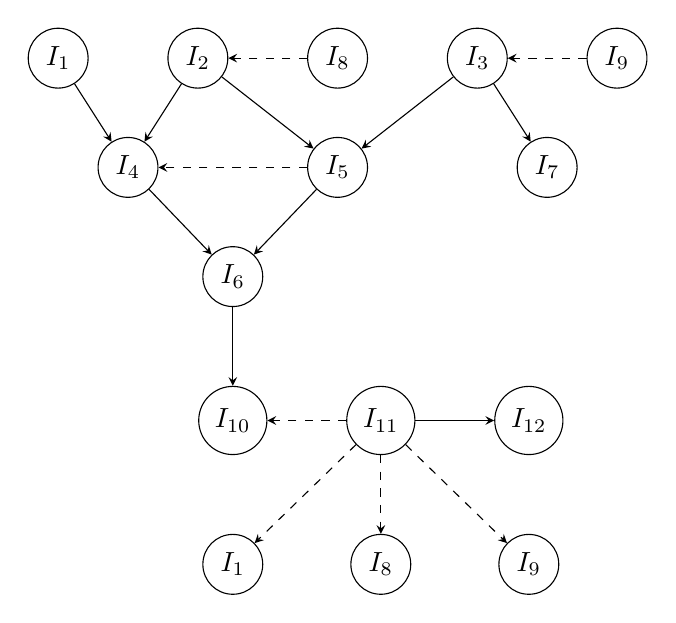
\begin{tikzpicture}[node distance=1cm, >=stealth]
        % Nodes
        \node[circle, draw] (I1) {$I_{1}$};
        \node[circle, draw, right=of I1] (I2) {$I_{2}$};
        \node[circle, draw, right=of I2] (I8) {$I_{8}$};
        \node[circle, draw, right=of I8] (I3) {$I_{3}$};
        \node[circle, draw, right=of I3] (I9) {$I_{9}$};

        \node[circle, draw, below=1cm of $(I1)!0.5!(I2)$] (I4) {$I_{4}$};
        \node[circle, draw, below=1cm of $(I2)!0.5!(I3)$] (I5) {$I_{5}$};
        \node[circle, draw, below=1cm of $(I3)!0.5!(I9)$] (I7) {$I_{7}$};

        \node[circle, draw, below=1cm of $(I4)!0.5!(I5)$] (I6) {$I_{6}$};

        \node[circle, draw, below=of I6] (I10) {$I_{10}$};
        \node[circle, draw, right=of I10] (I11) {$I_{11}$};
        \node[circle, draw, right=of I11] (I12) {$I_{12}$};

        \node[circle, draw, below=of I10] (I1_bis) {$I_{1}$};
        \node[circle, draw, below=of I11] (I8_bis) {$I_{8}$};
        \node[circle, draw, below=of I12] (I9_bis) {$I_{9}$};


        \draw[dashed, ->] (I5) -- (I4);
        \draw[dashed, ->] (I8) -- (I2);
        \draw[dashed, ->] (I9) -- (I3);
        \draw[dashed, ->] (I11) -- (I10);
        \draw[dashed, ->] (I11) -- (I1_bis);
        \draw[dashed, ->] (I11) -- (I8_bis);
        \draw[dashed, ->] (I11) -- (I9_bis);

        \draw[->] (I1) -- (I4);
        \draw[->] (I2) -- (I4);
        \draw[->] (I2) -- (I5);
        \draw[->] (I3) -- (I5);
        \draw[->] (I3) -- (I7);
        \draw[->] (I4) -- (I6);
        \draw[->] (I5) -- (I6);
        \draw[->] (I6) -- (I10);
        \draw[->] (I11) -- (I12);
    \end{tikzpicture}
\end{center}

\newpage

\begin{table}[!htp]
    \centering
    \begin{tabular}{@{} l | l | l | l @{}}
        \toprule
        & \textbf{Memory Unit} & \textbf{Floating Point Unit} & \textbf{Integer Unit} \\
        \midrule
        \textbf{C1}  & \texttt{LD F1, A(R1)} & & \\ [.3em]
        \textbf{C2}  & \texttt{LD F2, A(R2)} & & \texttt{ADDUI R2, R1, 8} \\ [.3em]
        \textbf{C3}  & \texttt{LD F3, A(R3)} & & \texttt{ADDUI R3, R1, 8} \\ [.3em]
        \textbf{C4}  & & & \\ [.3em]
        \textbf{C5}  & & \texttt{FADD F1, F1, F2} & \\ [.3em]
        \textbf{C6}  & & \texttt{FADD F2, F2, F3} & \\ [.3em]
        \textbf{C7}  & & \texttt{FADD F3, F3, F3} & \\ [.3em]
        \textbf{C8}  & & \texttt{FADD F1, F1, F2} & \\ [.3em]
        \textbf{C9}  & & & \\ [.3em]
        \textbf{C10}  & \texttt{SD F1, B(R1)} & & \texttt{ADDUI R1, R1, 4} \\ [.3em]
        \textbf{C11}  & & & \\ [.3em]
        \textbf{C12}  & & & \texttt{BNE R1, R2, LOOP} \\ [.3em]
        \textbf{C13}  & & & (delay slot) \\ [.3em]
        \textbf{C14}  & & & \\ [.3em]
        \textbf{C15}  & & & \\
        \bottomrule
    \end{tabular}
\end{table}

\begin{enumerate}
    \item \emph{How long is the critical path?}

    \answer The critical path is determined by the latency of the last instruction, \texttt{BNE}, so it is \textbf{13}.


    \item \emph{How much is the code efficiency?}

    \answer Efficiency is measured as follows:
    \begin{equation*}
        \text{Efficiency} = \dfrac{\text{Instruction Count}}{\text{\# cycles} \times \text{\# issues}} = \dfrac{12}{13 \cdot 3} = 0.307692308 = 30.77 \%
    \end{equation*}
\end{enumerate}

\newpage

\subsubsection*{Exercise 3 - MESI Protocol}

Let's consider the following access patterns on a \textbf{4-processor} system with a direct-mapped, write-back cache with one cache block per processor and a two-cache block memory.

\highspace
Assume the \textbf{MESI protocol} is used with \textbf{write-back} caches, \textbf{write-allocate}, and \textbf{write-invalidate} of other caches. \emph{Please COMPLETE the following table:}

\begin{table}[!htp]
    \centering
    \begin{adjustbox}{width={\textwidth},totalheight={\textheight},keepaspectratio}
        \begin{tabular}{@{} l l p{4em} p{4em} p{4em} p{4em} p{3em} p{3em} @{}}
            \toprule
            \textbf{Cycle} & \textbf{After Op.} & \textbf{P0 cache block state} & \textbf{P1 cache block state} & \textbf{P2 cache block state} & \textbf{P3 cache block state} & \textbf{Mem. at bl. 0 up to date?} & \textbf{Mem. at bl. 1 up to date?} \\
            \midrule
            1   & P0: Read Bl. 1    & Excl (1)  & Invalid   & Invalid   & Invalid   & Yes   & Yes   \\ [.3em]
            2   & P2: Read Bl. 0    & Excl (1)  & Invalid   & Excl (0)  & Invalid   & Yes   & Yes   \\ [.3em]
            3   & P3: Read Bl. 0    &           &           &           &           &       &       \\ [.3em]
            4   & P1: Write Bl. 0   &           &           &           &           &       &       \\ [.3em]
            5   & P0: Write Bl. 1   &           &           &           &           &       &       \\ [.3em]
            6   & P3: Read Bl. 1    &           &           &           &           &       &       \\
            \bottomrule
        \end{tabular}
    \end{adjustbox}
\end{table}

\noindent
\answer \definition{MESI} is a \textbf{cache coherence protocol}. It guarantees that multiple caches in a \textbf{shared-memory multiprocessor} see a \textbf{coherent view} of main memory.

\highspace
\textcolor{Green3}{\faIcon{question-circle} \textbf{Why is it needed?}} When multiple processors have private caches and share a memory space, they may each hold \emph{local copies} of the same memory block. If one processor modifies its copy, the other copies may become \textbf{stale} (incoherent). The MESI protocol ensures that all copies are kept consistent, meaning we never use an old value when we shouldn't.

\highspace
\textcolor{Green3}{\faIcon{book} \textbf{MESI States}} Each block in a cache can be in one of \textbf{4 states}:
\begin{itemize}
    \item \important{M} (\textbf{Modified}): Block is valid, \emph{dirty} (modified). It \emph{differs} from main memory. This cache \emph{owns} the latest value.
    \item \important{E} (\textbf{Exclusive}): Block is valid, \emph{clean}. It matches memory. This cache is the \emph{only} owner.
    \item \important{S} (\textbf{Shared}): Block is valid, clean, and may be in \emph{multiple} caches. All have the same value as memory.
    \item \important{I} (\textbf{Invalid}): Block is \emph{not} valid in this cache. Must be fetched on access.
\end{itemize}
\textbf{Coherence is enforced by invalidating or updating other caches}:
\begin{itemize}
    \item If a cache writes to a block, it must invalidate all other caches that have that block (\definitionWithSpecificIndex{Write-Invalidate}{Cache Write-Invalidate}{}).
    \item If a cache needs a block held dirty by another, that cache must supply the up-to-date data (and possibly write back to memory).
\end{itemize}
\textcolor{Green3}{\faIcon{question-circle} \textbf{What is Direct-Mapped Cache?}} \definition{Direct-Mapped} is the simplest cache mapping:
\begin{itemize}
    \item Each memory block maps to \textbf{exactly one} cache block.
    \item There's only one place in the cache where a given memory block can go.
\end{itemize}
In this exercise, each processor has a direct-mapped cache with \textbf{only one block}, so each processor can store \textbf{only one block at a time}.

\highspace
\textcolor{Green3}{\faIcon{question-circle} \textbf{What does Write-Back mean?}} Caches can be:
\begin{itemize}
    \item \definitionWithSpecificIndex{Write-Through}{Cache Write-Through}{}: Every write to the cache is also immediately written to main memory. Simpler, but more traffic.
    \item \definitionWithSpecificIndex{Write-Back}{Cache Write-Back}{}: Writes go only to the cache at first. The block is marked \emph{dirty}. The updated block is written back to main memory only when it is \emph{evicted} or needed by another processor.
\end{itemize}
In MESI: The \textbf{Modified (M)} state marks blocks that are \emph{dirty}. These blocks must be written back before eviction or when another processor requests them.

\highspace
\textcolor{Green3}{\faIcon{question-circle} \textbf{What does Write-Allocate mean?}} \definition{Write-Allocate} means that when a processor writes to a block that is not present in its cache (\emph{write miss}), it:
\begin{itemize}
    \item \textbf{Allocates}: It \emph{loads} the block into its cache.
    \item Then performs the write in the cache.
\end{itemize}
This is typical with write-back caches: the block must be in the cache so that it can later be written back to memory if needed.

\highspace
\textcolor{Green3}{\faIcon{question-circle} \textbf{What does ``One cache block per processor'' mean?}} In this exercise:
\begin{itemize}
    \item Each processor has \textbf{one slot in its cache}.
    \item That slot can hold \emph{one memory block} at a time.
    \item So if a processor needs to read/write a new block, it may need to \emph{evict} the old one (and write it back if it's dirty).
\end{itemize}
\textcolor{Green3}{\faIcon{question-circle} \textbf{What does ``Two-cache-block memory'' mean?}} This means that \textbf{main memory} has \textbf{only 2 data blocks} available: \textbf{block 0} and \textbf{block 1}. So:
\begin{itemize}
    \item The whole example focuses only on those two blocks.
    \item Any cache action involves either block 0 or block 1.
    \item The goal is to track how these two blocks move between the processors' caches and the main memory.
\end{itemize}

\newpage

\noindent
In summary, the entire scenario is as follows:
\begin{itemize}
    \item A \emph{tiny system} with 4 processors.
    \item Each has a \emph{tiny cache} (1 block).
    \item The system has only 2 memory blocks.
    \item Using MESI, caches cooperate to keep shared blocks consistent.
    \item \emph{Write-back}: modified blocks may not immediately update memory.
    \item \emph{Write-allocate}: writes on misses bring the block in.
\end{itemize}
\begin{enumerate}
    \setcounter{enumi}{-1}
    \item In the \textbf{initial state}, everything is up to date, but each block is invalid.


    \item \textbf{Operation \theenumi}: ``\texttt{P0: Read block 1}''. Since all the blocks are invalid, this is a \emph{cache miss} operation. Therefore, processor 0 (\texttt{P0}) loads block 1 from memory. Since no one else has it, the state is \textbf{Exclusive}. The memory is still up to date because it was ``\emph{read-by}'', not ``\emph{written-to}''.

    \begin{table}[!htp]
        \centering
        \begin{adjustbox}{width={\textwidth},totalheight={\textheight},keepaspectratio}
            \begin{tabular}{@{} l l p{4em} p{4em} p{4em} p{4em} p{3em} p{3em} @{}}
                \toprule
                \textbf{Cycle} & \textbf{After Op.} & \textbf{P0 cache block state} & \textbf{P1 cache block state} & \textbf{P2 cache block state} & \textbf{P3 cache block state} & \textbf{Mem. at bl. 0 up to date?} & \textbf{Mem. at bl. 1 up to date?} \\
                \midrule
                0   &                   & Invalid   & Invalid   & Invalid   & Invalid   & Yes   & Yes   \\ [.3em]
                1   & P0: Read Bl. 1    & Excl (1)  & Invalid   & Invalid   & Invalid   & Yes   & Yes   \\
                \bottomrule
            \end{tabular}
        \end{adjustbox}
    \end{table}


    \item \textbf{Operation \theenumi}: ``\texttt{P2: Read Bl. 0}''. Processor 2 has an invalid cache block, resulting in a \emph{cache miss}. Since nobody else has block 0, processor 2 loads it. It gets it in \textbf{Exclusive} mode. Again, the memory is up to date because it was read.

    \begin{table}[!htp]
        \centering
        \begin{adjustbox}{width={\textwidth},totalheight={\textheight},keepaspectratio}
            \begin{tabular}{@{} l l p{4em} p{4em} p{4em} p{4em} p{3em} p{3em} @{}}
                \toprule
                \textbf{Cycle} & \textbf{After Op.} & \textbf{P0 cache block state} & \textbf{P1 cache block state} & \textbf{P2 cache block state} & \textbf{P3 cache block state} & \textbf{Mem. at bl. 0 up to date?} & \textbf{Mem. at bl. 1 up to date?} \\
                \midrule
                0   &                   & Invalid   & Invalid   & Invalid   & Invalid   & Yes   & Yes   \\ [.3em]
                1   & P0: Read Bl. 1    & Excl (1)  & Invalid   & Invalid   & Invalid   & Yes   & Yes   \\ [.3em]
                2   & P2: Read Bl. 0    & Excl (1)  & Invalid   & Excl (0)  & Invalid   & Yes   & Yes   \\
                \bottomrule
            \end{tabular}
        \end{adjustbox}
    \end{table}


    \newpage


    \item \textbf{Operation \theenumi}: ``\texttt{P3: Read Bl. 0}''. Processor 3 has an invalid cache block, resulting in a \emph{cache miss}. This time, however, a copy of block 0 is in processor 2's cache, so processor 3 can request a copy of it. Now, since the value of block 0 is shared by different caches, we transition from \textbf{Exclusive} to \textbf{Shared}. Finally, the memory remains updated (no writes).

    \begin{table}[!htp]
        \centering
        \begin{adjustbox}{width={\textwidth},totalheight={\textheight},keepaspectratio}
            \begin{tabular}{@{} l l p{4em} p{4em} p{4em} p{4em} p{3em} p{3em} @{}}
                \toprule
                \textbf{Cycle} & \textbf{After Op.} & \textbf{P0 cache block state} & \textbf{P1 cache block state} & \textbf{P2 cache block state} & \textbf{P3 cache block state} & \textbf{Mem. at bl. 0 up to date?} & \textbf{Mem. at bl. 1 up to date?} \\
                \midrule
                0   &                   & Invalid   & Invalid   & Invalid   & Invalid   & Yes   & Yes   \\ [.3em]
                1   & P0: Read Bl. 1    & Excl (1)  & Invalid   & Invalid   & Invalid   & Yes   & Yes   \\ [.3em]
                2   & P2: Read Bl. 0    & Excl (1)  & Invalid   & Excl (0)  & Invalid   & Yes   & Yes   \\ [.3em]
                3   & P3: Read Bl. 0    & Excl (1)  & Invalid   & Shr (0)   & Shr (0)   & Yes   & Yes   \\
                \bottomrule
            \end{tabular}
        \end{adjustbox}
    \end{table}


    \item \textbf{Operation \theenumi}: ``\texttt{P1: Write Bl. 0}''. Since Processor 1 does not have Block 0, there is a cache miss. Block 0 is in processors 2 and 3's caches in Shared mode. So, MESI:
    \begin{enumerate}
        \item P1 needs exclusive access, so it invalidates all other copies.
        \item P2 and P3 are invalidated by P1 and become invalid.
        \item P1 loads block 0, writes it, and transitions from \textbf{Exclusive} to \textbf{Modified}.
    \end{enumerate}
    Since it's write-back, the memory for block 0 becomes stale (marked as out-of-date).

    \begin{table}[!htp]
        \centering
        \begin{adjustbox}{width={\textwidth},totalheight={\textheight},keepaspectratio}
            \begin{tabular}{@{} l l p{4em} p{4em} p{4em} p{4em} p{3em} p{3em} @{}}
                \toprule
                \textbf{Cycle} & \textbf{After Op.} & \textbf{P0 cache block state} & \textbf{P1 cache block state} & \textbf{P2 cache block state} & \textbf{P3 cache block state} & \textbf{Mem. at bl. 0 up to date?} & \textbf{Mem. at bl. 1 up to date?} \\
                \midrule
                0   &                   & Invalid   & Invalid   & Invalid   & Invalid   & Yes   & Yes   \\ [.3em]
                1   & P0: Read Bl. 1    & Excl (1)  & Invalid   & Invalid   & Invalid   & Yes   & Yes   \\ [.3em]
                2   & P2: Read Bl. 0    & Excl (1)  & Invalid   & Excl (0)  & Invalid   & Yes   & Yes   \\ [.3em]
                3   & P3: Read Bl. 0    & Excl (1)  & Invalid   & Shr (0)   & Shr (0)   & Yes   & Yes   \\ [.3em]
                4   & P1: Write Bl. 0   & Excl (1)  & Mod (0)   & Invalid   & Invalid   & No    & Yes   \\
                \bottomrule
            \end{tabular}
        \end{adjustbox}
    \end{table}


    \newpage


    \item \textbf{Operation \theenumi}: ``\texttt{P0: Write Bl. 1}''. Processor 0 already has Block 1 in \textbf{Exclusive} mode. When it writes, it switches from Exclusive to \textbf{Modified} mode. Because a write was made, the memory is no longer up to date. Since no one has block 1, it doesn't invalidate the other caches.

    \begin{table}[!htp]
        \centering
        \begin{adjustbox}{width={\textwidth},totalheight={\textheight},keepaspectratio}
            \begin{tabular}{@{} l l p{4em} p{4em} p{4em} p{4em} p{3em} p{3em} @{}}
                \toprule
                \textbf{Cycle} & \textbf{After Op.} & \textbf{P0 cache block state} & \textbf{P1 cache block state} & \textbf{P2 cache block state} & \textbf{P3 cache block state} & \textbf{Mem. at bl. 0 up to date?} & \textbf{Mem. at bl. 1 up to date?} \\
                \midrule
                0   &                   & Invalid   & Invalid   & Invalid   & Invalid   & Yes   & Yes   \\ [.3em]
                1   & P0: Read Bl. 1    & Excl (1)  & Invalid   & Invalid   & Invalid   & Yes   & Yes   \\ [.3em]
                2   & P2: Read Bl. 0    & Excl (1)  & Invalid   & Excl (0)  & Invalid   & Yes   & Yes   \\ [.3em]
                3   & P3: Read Bl. 0    & Excl (1)  & Invalid   & Shr (0)   & Shr (0)   & Yes   & Yes   \\ [.3em]
                4   & P1: Write Bl. 0   & Excl (1)  & Mod (0)   & Invalid   & Invalid   & No    & Yes   \\ [.3em]
                5   & P0: Write Bl. 1   & Mod (1)   & Mod (0)   & Invalid   & Invalid   & No    & No   \\
                \bottomrule
            \end{tabular}
        \end{adjustbox}
    \end{table}


    \item \textbf{Operation \theenumi}: ``\texttt{P3: Read Bl. 1}''. Since processor 3 does not have block 1, there is a \emph{cache miss}. Processor 0 has block 1 in modified mode.
    \begin{enumerate}
        \item Another processor needs the data.
        \item P0 must supply the \emph{latest value}, so P0 does \emph{write-back} or sends directly.
        \item Result: P3 loads up-to-date block, and both now have it in \textbf{Shared}.
    \end{enumerate}
    Now the memory for block 1 is clean again (assuming P0 did a write-back).

    \begin{table}[!htp]
        \centering
        \begin{adjustbox}{width={\textwidth},totalheight={\textheight},keepaspectratio}
            \begin{tabular}{@{} l l p{4em} p{4em} p{4em} p{4em} p{3em} p{3em} @{}}
                \toprule
                \textbf{Cycle} & \textbf{After Op.} & \textbf{P0 cache block state} & \textbf{P1 cache block state} & \textbf{P2 cache block state} & \textbf{P3 cache block state} & \textbf{Mem. at bl. 0 up to date?} & \textbf{Mem. at bl. 1 up to date?} \\
                \midrule
                0   &                   & Invalid   & Invalid   & Invalid   & Invalid   & Yes   & Yes   \\ [.3em]
                1   & P0: Read Bl. 1    & Excl (1)  & Invalid   & Invalid   & Invalid   & Yes   & Yes   \\ [.3em]
                2   & P2: Read Bl. 0    & Excl (1)  & Invalid   & Excl (0)  & Invalid   & Yes   & Yes   \\ [.3em]
                3   & P3: Read Bl. 0    & Excl (1)  & Invalid   & Shr (0)   & Shr (0)   & Yes   & Yes   \\ [.3em]
                4   & P1: Write Bl. 0   & Excl (1)  & Mod (0)   & Invalid   & Invalid   & No    & Yes   \\ [.3em]
                5   & P0: Write Bl. 1   & Mod (1)   & Mod (0)   & Invalid   & Invalid   & No    & No    \\ [.3em]
                6   & P3: Read Bl. 1    & Shr (1)   & Mod (0)   & Invalid   & Shr (1)   & No    & Yes   \\
                \bottomrule
            \end{tabular}
        \end{adjustbox}
    \end{table}
\end{enumerate}
Note: Read from \textbf{Modified} forces a write-back (or direct transfer) to maintain consistency.

\newpage

\subsubsection*{Exercise 4 - Reordered Buffer}

\emph{Let's consider the following assembly loop where registers \textbf{\texttt{\$R1}} and \textbf{\texttt{\$R2}} are initialized at 0 and 40 respectively:}
\begin{lstlisting}[mathescape=false]
L0:     LD $F2, 0 ($R1)
L1:     ADDD $F4, $F2, $F2
L2:     SD $F4, 0 ($R1)
L3:     ADDI $R1, $R1, 4
L4:     BNE $R1, $R2, L0 # branch predicted as taken
\end{lstlisting}
\begin{itemize}
    \item \emph{How many loop iterations?}

    \answer The register \texttt{R1} is incremented by 4 at each iteration:
    \begin{equation*}
        \text{Iterations} = \dfrac{40}{4} = 10
    \end{equation*}


    \item \emph{How many instructions per iteration?}

    \answer 5 instructions.


    \item \emph{How many control vs datapath instructions?}

    \answer To answer the question, we count \textbf{how many instructions in the loop control the flow} vs \textbf{how many do actual data processing}. In our loop:
    \begin{lstlisting}[language=unknown]
L0:     LD $F2, 0($R1)         # datapath: load data
L1:     ADDD $F4, $F2, $F2     # datapath: compute
L2:     SD $F4, 0($R1)         # datapath: store data
L3:     ADDI $R1, $R1, 4       # control: index update
L4:     BNE $R1, $R2, L0       # control: conditional branch\end{lstlisting}
    \begin{itemize}
        \item \textbf{Data path instructions}: \texttt{LD}, \texttt{ADDD}, \texttt{SD}, 3 instructions.
        \item \textbf{Control instructions}: \texttt{ADDI} (updates loop index), \texttt{BNE} (branch), 2 instructions.
    \end{itemize}
    So, the answer is \hl{2 control vs 3 datapath instructions}. In general:
    \begin{itemize}
        \item \textbf{Control instructions}: branches, jumps, index updates.
        \item \textbf{Datapath instructions}: load, store, ALU/FPU operations that compute or move data.
    \end{itemize}
\end{itemize}

\newpage

\noindent
Write the unrolled version of the loop with unrolling factor 2 by using Register Renaming.

\highspace
\answer
\begin{lstlisting}[language=unknown]
L0:     LD $F2, 0($R1)         # datapath: load data
L1:     ADDD $F4, $F2, $F2     # datapath: compute
L2:     SD $F4, 0($R1)         # datapath: store data
L3:     LD $F6, 4($R1)         # datapath: load data
L4:     ADDD $F8, $F6, $F6     # datapath: compute
L5:     SD $F8, 0($R1)         # datapath: store data
L6:     ADDI $R1, $R1, 8       # control: index update
L7:     BNE $R1, $R2, L0       # control: conditional branch\end{lstlisting}
\begin{itemize}
    \item \emph{How many loop iterations?}

    \answer The register \texttt{R1} is incremented by 8 at each iteration:
    \begin{equation*}
        \text{Iterations} = \dfrac{40}{8} = 5
    \end{equation*}


    \item \emph{How many instructions per iteration?}

    \answer 8 instructions.


    \item \emph{How many control vs datapath instructions?}

    \answer 2 control vs 6 datapath instructions.
\end{itemize}
\emph{Execute the unrolled version of the loop by the \textbf{Speculative Tomasulo} architecture with a 10-entry ROB and:
\begin{itemize}
    \item 4 Load Buffers (Load1, Load2, Load3, Load4);
    \item 4 FP Reservation Stations (FP1, FP2, FP3, FP4)
    \item 2 Integer Reservation Stations (Int1, Int2)
\end{itemize}
Complete the ROB and the Rename Table until the ROB becomes \textbf{full} while the first instruction is still in execution due to a cache miss (*):}
\begin{table}[!htp]
    \centering
    \begin{adjustbox}{width={\textwidth},totalheight={\textheight},keepaspectratio}
        \begin{tabular}{@{} l l l l l l @{}}
            \toprule
            \texttt{ROB\#}  & \textbf{Instruction} & \textbf{Dest.} & \textbf{Res. Alloc.} & \textbf{Ready/Status} & \textbf{Spec.} \\
            \midrule
            \texttt{ROB0}   & \texttt{L0: LD \$F2, 0 (\$R1)}    & \texttt{\$F2} & \texttt{Load1}    & No, exec.(*)  & No    \\ [.3em]
            \texttt{ROB1}   & \texttt{L1: ADDD \$F4, \$F2, \$F2}& \texttt{\$F4} & \texttt{FP1}      & No, issued    & No    \\ [.3em]
            \texttt{ROB2}   &                                   &               &                   &               &       \\ [.3em]
            \texttt{ROB3}   &                                   &               &                   &               &       \\ [.3em]
            \texttt{ROB4}   &                                   &               &                   &               &       \\ [.3em]
            \texttt{ROB5}   &                                   &               &                   &               &       \\ [.3em]
            \texttt{ROB6}   &                                   &               &                   &               &       \\ [.3em]
            \texttt{ROB7}   &                                   &               &                   &               &       \\ [.3em]
            \texttt{ROB8}   &                                   &               &                   &               &       \\ [.3em]
            \texttt{ROB9}   &                                   &               &                   &               &       \\
            \bottomrule
        \end{tabular}
    \end{adjustbox}
    \caption*{\emph{\textbf{ROB Table}}}
\end{table}

\newpage

\begin{table}[!htp]
    \centering
    \begin{tabular}{@{} l l @{}}
        \toprule
        \texttt{Reg \#}  & \texttt{ROB \#} \\
        \midrule
        \texttt{\$F0}    & \texttt{--} \\ [.3em]
        \texttt{\$F2}    & \\ [.3em]
        \texttt{\$F4}    & \\ [.3em]
        \texttt{\$F6}    & \\ [.3em]
        \texttt{\$F8}    & \\
        \bottomrule
    \end{tabular}
    \caption*{\emph{\textbf{Rename Table}}}
\end{table}

\highspace
\answer
\begin{enumerate}
    \item First, we allocate the entries given by the exercise in the Rename Table:
    \begin{table}[!htp]
        \centering
        \begin{tabular}{@{} l l @{}}
            \toprule
            \texttt{Reg \#}  & \texttt{ROB \#} \\
            \midrule
            \texttt{\$F0}    & \texttt{--} \\ [.3em]
            \texttt{\$F2}    & \texttt{ROB0} \\ [.3em]
            \texttt{\$F4}    & \texttt{ROB1} \\ [.3em]
            \texttt{\$F6}    & \\ [.3em]
            \texttt{\$F8}    & \\
            \bottomrule
        \end{tabular}
        \caption*{\emph{\textbf{Rename Table}}}
    \end{table}


    \item We issue the \texttt{L2} instruction. The operation's destination is memory. The status has not been issued yet because we are filling the ROB due to a cache miss, and the processor is waiting for the result of the operation.
    \begin{table}[!htp]
        \centering
        \begin{adjustbox}{width={\textwidth},totalheight={\textheight},keepaspectratio}
            \begin{tabular}{@{} l l l l l l @{}}
                \toprule
                \texttt{ROB\#}  & \textbf{Instruction} & \textbf{Dest.} & \textbf{Res. Alloc.} & \textbf{Ready/Status} & \textbf{Spec.} \\
                \midrule
                \texttt{ROB0}   & \texttt{L0: LD \$F2, 0 (\$R1)}    & \texttt{\$F2} & \texttt{Load1}    & No, exec.(*)  & No    \\ [.3em]
                \texttt{ROB1}   & \texttt{L1: ADDD \$F4, \$F2, \$F2}& \texttt{\$F4} & \texttt{FP1}      & No, issued    & No    \\ [.3em]
                \texttt{ROB2}   & \texttt{L2: SD \$F4, 0(\$R1)}     & \texttt{Mem}  & \texttt{--}       & No, issued    & No    \\ [.3em]
                \texttt{ROB3}   &                                   &               &                   &               &       \\ [.3em]
                \texttt{ROB4}   &                                   &               &                   &               &       \\ [.3em]
                \texttt{ROB5}   &                                   &               &                   &               &       \\ [.3em]
                \texttt{ROB6}   &                                   &               &                   &               &       \\ [.3em]
                \texttt{ROB7}   &                                   &               &                   &               &       \\ [.3em]
                \texttt{ROB8}   &                                   &               &                   &               &       \\ [.3em]
                \texttt{ROB9}   &                                   &               &                   &               &       \\
                \bottomrule
            \end{tabular}
        \end{adjustbox}
        \caption*{\emph{\textbf{ROB Table}}}
    \end{table}

    
    \newpage


    \item We issue the \texttt{L3} instruction. The destination is the left operand, register \texttt{F6}. We use \texttt{Load 2} as the functional unit.
    \begin{table}[!htp]
        \centering
        \begin{adjustbox}{width={\textwidth},totalheight={\textheight},keepaspectratio}
            \begin{tabular}{@{} l l l l l l @{}}
                \toprule
                \texttt{ROB\#}  & \textbf{Instruction} & \textbf{Dest.} & \textbf{Res. Alloc.} & \textbf{Ready/Status} & \textbf{Spec.} \\
                \midrule
                \texttt{ROB0}   & \texttt{L0: LD \$F2, 0 (\$R1)}    & \texttt{\$F2} & \texttt{Load1}    & No, exec.(*)  & No    \\ [.3em]
                \texttt{ROB1}   & \texttt{L1: ADDD \$F4, \$F2, \$F2}& \texttt{\$F4} & \texttt{FP1}      & No, issued    & No    \\ [.3em]
                \texttt{ROB2}   & \texttt{L2: SD \$F4, 0(\$R1)}     & \texttt{Mem}  & \texttt{--}       & No, issued    & No    \\ [.3em]
                \texttt{ROB3}   & \texttt{L3: LD \$F6, 4(\$R1)}     & \texttt{\$F6} & \texttt{Load2}    & No, issued    & No    \\ [.3em]
                \texttt{ROB4}   &                                   &               &                   &               &       \\ [.3em]
                \texttt{ROB5}   &                                   &               &                   &               &       \\ [.3em]
                \texttt{ROB6}   &                                   &               &                   &               &       \\ [.3em]
                \texttt{ROB7}   &                                   &               &                   &               &       \\ [.3em]
                \texttt{ROB8}   &                                   &               &                   &               &       \\ [.3em]
                \texttt{ROB9}   &                                   &               &                   &               &       \\
                \bottomrule
            \end{tabular}
        \end{adjustbox}
        \caption*{\emph{\textbf{ROB Table}}}
    \end{table}
    \begin{table}[!htp]
        \centering
        \begin{tabular}{@{} l l @{}}
            \toprule
            \texttt{Reg \#}  & \texttt{ROB \#} \\
            \midrule
            \texttt{\$F0}    & \texttt{--} \\ [.3em]
            \texttt{\$F2}    & \texttt{ROB0} \\ [.3em]
            \texttt{\$F4}    & \texttt{ROB1} \\ [.3em]
            \texttt{\$F6}    & \texttt{ROB3} \\ [.3em]
            \texttt{\$F8}    & \\
            \bottomrule
        \end{tabular}
        \caption*{\emph{\textbf{Rename Table}}}
    \end{table}


    \newpage


    \item We issue the \texttt{L4} instruction.
    \begin{table}[!htp]
        \centering
        \begin{adjustbox}{width={\textwidth},totalheight={\textheight},keepaspectratio}
            \begin{tabular}{@{} l l l l l l @{}}
                \toprule
                \texttt{ROB\#}  & \textbf{Instruction} & \textbf{Dest.} & \textbf{Res. Alloc.} & \textbf{Ready/Status} & \textbf{Spec.} \\
                \midrule
                \texttt{ROB0}   & \texttt{L0: LD \$F2, 0 (\$R1)}    & \texttt{\$F2} & \texttt{Load1}    & No, exec.(*)  & No    \\ [.3em]
                \texttt{ROB1}   & \texttt{L1: ADDD \$F4, \$F2, \$F2}& \texttt{\$F4} & \texttt{FP1}      & No, issued    & No    \\ [.3em]
                \texttt{ROB2}   & \texttt{L2: SD \$F4, 0(\$R1)}     & \texttt{Mem}  & \texttt{--}       & No, issued    & No    \\ [.3em]
                \texttt{ROB3}   & \texttt{L3: LD \$F6, 4(\$R1)}     & \texttt{\$F6} & \texttt{Load2}    & No, issued    & No    \\ [.3em]
                \texttt{ROB4}   & \texttt{L4: ADDD \$F8, \$F6, \$F6}& \texttt{\$F8} & \texttt{FP2}      & No, issued    & No    \\ [.3em]
                \texttt{ROB5}   &                                   &               &                   &               &       \\ [.3em]
                \texttt{ROB6}   &                                   &               &                   &               &       \\ [.3em]
                \texttt{ROB7}   &                                   &               &                   &               &       \\ [.3em]
                \texttt{ROB8}   &                                   &               &                   &               &       \\ [.3em]
                \texttt{ROB9}   &                                   &               &                   &               &       \\
                \bottomrule
            \end{tabular}
        \end{adjustbox}
        \caption*{\emph{\textbf{ROB Table}}}
    \end{table}
    \begin{table}[!htp]
        \centering
        \begin{tabular}{@{} l l @{}}
            \toprule
            \texttt{Reg \#}  & \texttt{ROB \#} \\
            \midrule
            \texttt{\$F0}    & \texttt{--} \\ [.3em]
            \texttt{\$F2}    & \texttt{ROB0} \\ [.3em]
            \texttt{\$F4}    & \texttt{ROB1} \\ [.3em]
            \texttt{\$F6}    & \texttt{ROB3} \\ [.3em]
            \texttt{\$F8}    & \texttt{ROB4} \\
            \bottomrule
        \end{tabular}
        \caption*{\emph{\textbf{Rename Table}}}
    \end{table}


    \item We issue the \texttt{L5} instruction.
    \begin{table}[!htp]
        \centering
        \begin{adjustbox}{width={\textwidth},totalheight={\textheight},keepaspectratio}
            \begin{tabular}{@{} l l l l l l @{}}
                \toprule
                \texttt{ROB\#}  & \textbf{Instruction} & \textbf{Dest.} & \textbf{Res. Alloc.} & \textbf{Ready/Status} & \textbf{Spec.} \\
                \midrule
                \texttt{ROB0}   & \texttt{L0: LD \$F2, 0 (\$R1)}    & \texttt{\$F2} & \texttt{Load1}    & No, exec.(*)  & No    \\ [.3em]
                \texttt{ROB1}   & \texttt{L1: ADDD \$F4, \$F2, \$F2}& \texttt{\$F4} & \texttt{FP1}      & No, issued    & No    \\ [.3em]
                \texttt{ROB2}   & \texttt{L2: SD \$F4, 0(\$R1)}     & \texttt{Mem}  & \texttt{--}       & No, issued    & No    \\ [.3em]
                \texttt{ROB3}   & \texttt{L3: LD \$F6, 4(\$R1)}     & \texttt{\$F6} & \texttt{Load2}    & No, issued    & No    \\ [.3em]
                \texttt{ROB4}   & \texttt{L4: ADDD \$F8, \$F6, \$F6}& \texttt{\$F8} & \texttt{FP2}      & No, issued    & No    \\ [.3em]
                \texttt{ROB5}   & \texttt{L5: SD \$F8, 0(\$R1)}     & \texttt{Mem}  & \texttt{--}       & No, issued    & No    \\ [.3em]
                \texttt{ROB6}   &                                   &               &                   &               &       \\ [.3em]
                \texttt{ROB7}   &                                   &               &                   &               &       \\ [.3em]
                \texttt{ROB8}   &                                   &               &                   &               &       \\ [.3em]
                \texttt{ROB9}   &                                   &               &                   &               &       \\
                \bottomrule
            \end{tabular}
        \end{adjustbox}
        \caption*{\emph{\textbf{ROB Table}}}
    \end{table}


    \newpage


    \item We issue the \texttt{L6} instruction.
    \begin{table}[!htp]
        \centering
        \begin{adjustbox}{width={\textwidth},totalheight={\textheight},keepaspectratio}
            \begin{tabular}{@{} l l l l l l @{}}
                \toprule
                \texttt{ROB\#}  & \textbf{Instruction} & \textbf{Dest.} & \textbf{Res. Alloc.} & \textbf{Ready/Status} & \textbf{Spec.} \\
                \midrule
                \texttt{ROB0}   & \texttt{L0: LD \$F2, 0 (\$R1)}    & \texttt{\$F2} & \texttt{Load1}    & No, exec.(*)  & No    \\ [.3em]
                \texttt{ROB1}   & \texttt{L1: ADDD \$F4, \$F2, \$F2}& \texttt{\$F4} & \texttt{FP1}      & No, issued    & No    \\ [.3em]
                \texttt{ROB2}   & \texttt{L2: SD \$F4, 0(\$R1)}     & \texttt{Mem}  & \texttt{--}       & No, issued    & No    \\ [.3em]
                \texttt{ROB3}   & \texttt{L3: LD \$F6, 4(\$R1)}     & \texttt{\$F6} & \texttt{Load2}    & No, issued    & No    \\ [.3em]
                \texttt{ROB4}   & \texttt{L4: ADDD \$F8, \$F6, \$F6}& \texttt{\$F8} & \texttt{FP2}      & No, issued    & No    \\ [.3em]
                \texttt{ROB5}   & \texttt{L5: SD \$F8, 0(\$R1)}     & \texttt{Mem}  & \texttt{--}       & No, issued    & No    \\ [.3em]
                \texttt{ROB6}   & \texttt{L6: ADDI \$R1, \$R1, 8}   & \texttt{\$R1} & \texttt{Int1}     & No, issued    & No    \\ [.3em]
                \texttt{ROB7}   &                                   &               &                   &               &       \\ [.3em]
                \texttt{ROB8}   &                                   &               &                   &               &       \\ [.3em]
                \texttt{ROB9}   &                                   &               &                   &               &       \\
                \bottomrule
            \end{tabular}
        \end{adjustbox}
        \caption*{\emph{\textbf{ROB Table}}}
    \end{table}


    \item We issue the \texttt{L7} instruction.
    \begin{table}[!htp]
        \centering
        \begin{adjustbox}{width={\textwidth},totalheight={\textheight},keepaspectratio}
            \begin{tabular}{@{} l l l l l l @{}}
                \toprule
                \texttt{ROB\#}  & \textbf{Instruction} & \textbf{Dest.} & \textbf{Res. Alloc.} & \textbf{Ready/Status} & \textbf{Spec.} \\
                \midrule
                \texttt{ROB0}   & \texttt{L0: LD \$F2, 0 (\$R1)}    & \texttt{\$F2} & \texttt{Load1}    & No, exec.(*)  & No    \\ [.3em]
                \texttt{ROB1}   & \texttt{L1: ADDD \$F4, \$F2, \$F2}& \texttt{\$F4} & \texttt{FP1}      & No, issued    & No    \\ [.3em]
                \texttt{ROB2}   & \texttt{L2: SD \$F4, 0(\$R1)}     & \texttt{Mem}  & \texttt{--}       & No, issued    & No    \\ [.3em]
                \texttt{ROB3}   & \texttt{L3: LD \$F6, 4(\$R1)}     & \texttt{\$F6} & \texttt{Load2}    & No, issued    & No    \\ [.3em]
                \texttt{ROB4}   & \texttt{L4: ADDD \$F8, \$F6, \$F6}& \texttt{\$F8} & \texttt{FP2}      & No, issued    & No    \\ [.3em]
                \texttt{ROB5}   & \texttt{L5: SD \$F8, 0(\$R1)}     & \texttt{Mem}  & \texttt{--}       & No, issued    & No    \\ [.3em]
                \texttt{ROB6}   & \texttt{L6: ADDI \$R1, \$R1, 8}   & \texttt{\$R1} & \texttt{Int1}     & No, issued    & No    \\ [.3em]
                \texttt{ROB7}   & \texttt{L7: BNE \$R1, \$R2, L0}   & \texttt{--}   & \texttt{Int2}     & No, issued    & No    \\ [.3em]
                \texttt{ROB8}   &                                   &               &                   &               &       \\ [.3em]
                \texttt{ROB9}   &                                   &               &                   &               &       \\
                \bottomrule
            \end{tabular}
        \end{adjustbox}
        \caption*{\emph{\textbf{ROB Table}}}
    \end{table}


    \newpage


    \item We issue \texttt{L0} and \texttt{L1}. Since we need to fill out the entire ROB table and we don't know whether the branch will be true or false, we made a prediction. Therefore, each speculative entry will be set to true.
    \begin{table}[!htp]
        \centering
        \begin{adjustbox}{width={\textwidth},totalheight={\textheight},keepaspectratio}
            \begin{tabular}{@{} l l l l l l @{}}
                \toprule
                \texttt{ROB\#}  & \textbf{Instruction} & \textbf{Dest.} & \textbf{Res. Alloc.} & \textbf{Ready/Status} & \textbf{Spec.} \\
                \midrule
                \texttt{ROB0}   & \texttt{L0: LD \$F2, 0 (\$R1)}    & \texttt{\$F2} & \texttt{Load1}    & No, exec.(*)  & No    \\ [.3em]
                \texttt{ROB1}   & \texttt{L1: ADDD \$F4, \$F2, \$F2}& \texttt{\$F4} & \texttt{FP1}      & No, issued    & No    \\ [.3em]
                \texttt{ROB2}   & \texttt{L2: SD \$F4, 0(\$R1)}     & \texttt{Mem}  & \texttt{--}       & No, issued    & No    \\ [.3em]
                \texttt{ROB3}   & \texttt{L3: LD \$F6, 4(\$R1)}     & \texttt{\$F6} & \texttt{Load2}    & No, issued    & No    \\ [.3em]
                \texttt{ROB4}   & \texttt{L4: ADDD \$F8, \$F6, \$F6}& \texttt{\$F8} & \texttt{FP2}      & No, issued    & No    \\ [.3em]
                \texttt{ROB5}   & \texttt{L5: SD \$F8, 0(\$R1)}     & \texttt{Mem}  & \texttt{--}       & No, issued    & No    \\ [.3em]
                \texttt{ROB6}   & \texttt{L6: ADDI \$R1, \$R1, 8}   & \texttt{\$R1} & \texttt{Int1}     & No, issued    & No    \\ [.3em]
                \texttt{ROB7}   & \texttt{L7: BNE \$R1, \$R2, L0}   & \texttt{--}   & \texttt{Int2}     & No, issued    & No    \\ [.3em]
                \texttt{ROB8}   & \texttt{L0: LD \$F2, 0(\$R1)}     & \texttt{\$F2} & \texttt{Load3}    & No, issued    & Yes   \\ [.3em]
                \texttt{ROB9}   & \texttt{L1: ADDD \$F4, \$F2, \$F2}& \texttt{\$F4} & \texttt{FP3}      & No, issued    & Yes   \\
                \bottomrule
            \end{tabular}
        \end{adjustbox}
        \caption*{\emph{\textbf{ROB Table}}}
    \end{table}
    \begin{table}[!htp]
        \centering
        \begin{tabular}{@{} l l @{}}
            \toprule
            \texttt{Reg \#}  & \texttt{ROB \#} \\
            \midrule
            \texttt{\$F0}    & \texttt{--} \\ [.3em]
            \texttt{\$F2}    & $\cancel{\texttt{ROB0}}$ \texttt{ROB8} \\ [.3em]
            \texttt{\$F4}    & $\cancel{\texttt{ROB1}}$ \texttt{ROB9} \\ [.3em]
            \texttt{\$F6}    & \texttt{ROB3} \\ [.3em]
            \texttt{\$F8}    & \texttt{ROB4} \\
            \bottomrule
        \end{tabular}
        \caption*{\emph{\textbf{Rename Table}}}
    \end{table}
\end{enumerate}


    %%%%%%%%%%%%%%%%%%%%%%%%%
    % Clear fancy pagestyle %
    %%%%%%%%%%%%%%%%%%%%%%%%%
    \pagestyle{fancy}
    \fancyhead{} % clear all header fields
    \fancyhead[R]{\nouppercase{\leftmark}}

    %%%%%%%%%%%%%%%%%%%%%%%%%%
    % Bibliography and index %
    %%%%%%%%%%%%%%%%%%%%%%%%%%
    \pagestyle{fancy}
\fancyhead{} % clear all header fields
\fancyhead[R]{\nouppercase{\leftmark\hfill\rightmark}}

\pagestyle{fancy}
\fancyhead{} % clear all header fields
\fancyhead[R]{\nouppercase{\leftmark}}

\bibliography{bibtex}{}
\bibliographystyle{plain}

\newpage

\printindex
\end{document}